% !TeX program = xelatex
% Compile với XeLaTeX (Overleaf: Menu > Compiler > XeLaTeX)
\documentclass[aspectratio=169,9pt]{beamer}

\usepackage{fontspec}
\setmainfont{Noto Serif}
\setsansfont{Noto Sans}
\usepackage{polyglossia}
\setmainlanguage{vietnamese}

\usepackage{amsmath,amssymb}
\usepackage{graphicx}
\usepackage{booktabs}
\usepackage{tikz}
\usetikzlibrary{arrows.meta,positioning,shapes,fit}
\usepackage{caption}
\captionsetup{font=scriptsize,labelfont=bf}
\usepackage{etoolbox}
\AtBeginEnvironment{itemize}{\setlength{\itemsep}{1pt}\setlength{\parskip}{0pt}\setlength{\topsep}{1pt}}
\AtBeginEnvironment{enumerate}{\setlength{\itemsep}{1pt}\setlength{\parskip}{0pt}\setlength{\topsep}{1pt}}
\setlength{\abovedisplayskip}{4pt}
\setlength{\belowdisplayskip}{4pt}
\setlength{\abovedisplayshortskip}{2pt}
\setlength{\belowdisplayshortskip}{2pt}

\usetheme{Madrid}
\usecolortheme{seahorse}
\setbeamertemplate{navigation symbols}{}
\setbeamertemplate{footline}[frame number]
\setbeamerfont{footnote}{size=\tiny}
\setbeamerfont{section in toc}{size=\tiny}
\setbeamerfont{subsection in toc}{size=\tiny}

\title[FastGS-lite: 3DGS \& Tăng tốc]{Quy trình Render 3D Gaussian Splatting\\và Cải tiến FastGS (FastGS-lite)}
\subtitle{Từ toán học nền tảng đến Adaptive Density Control chuyên sâu}
\author{Digital Twin GS}
\date{\today}

\graphicspath{{figures/}{../BOOK/fastergs_merge_figures/}{../BOOK/adc_figures/}}

\begin{document}

\begin{frame}
\titlepage
\end{frame}

\begin{frame}{Mục lục}
\tiny
\tableofcontents
\end{frame}

% ===================== PHẦN 1 =====================
\section{Nền tảng: 3D Gaussian là gì}
% --- Slide 1 ---
\begin{frame}
\titlepage
\end{frame}

% --- Slide 2 ---
\begin{frame}{Nội dung trình bày}
\begin{enumerate}
    \item Nền tảng: 3D Gaussian là gì
    \item Chiếu phối cảnh \& Rasterizer khả vi
    \item Loss, Metric, Gradient \& Optimizer
    \item Adaptive Density Control (Clone/Split/Prune)
    \item Ba đòn bẩy tăng tốc của FastGS
    \item FastGS-lite trên Colab T4: pipeline \& kết quả
    \item Quan sát, giới hạn \& kết luận
\end{enumerate}
\end{frame}

% --- Slide 3 ---
\begin{frame}{Động lực: vì sao cần một biểu diễn cảnh mới?}
\begin{itemize}
    \item NeRF (Neural Radiance Fields): biểu diễn \textbf{implicit} bằng MLP, chất lượng cao nhưng render rất chậm (giây/khung hình).
    \item 3D Gaussian Splatting (3DGS): biểu diễn \textbf{explicit} bằng hàng trăm nghìn ``quả cầu'' Gaussian mờ trong không gian.
    \item Render bằng \textbf{rasterization khả vi} (differentiable rasterizer) thay vì ray-marching qua mạng nơ-ron.
    \item Kết quả: tốc độ render đạt hàng chục--hàng trăm FPS, gần thời gian thực.
\end{itemize}
\vspace{0.3cm}
\small
\centering
\begin{tabular}{lll}
\toprule
\textbf{Tiêu chí} & \textbf{NeRF} & \textbf{3D Gaussian Splatting} \\
\midrule
Biểu diễn & Implicit (MLP) & Explicit (tập Gaussian) \\
Render & Ray-marching, chậm & Rasterization, nhanh \\
Tốc độ & $\sim$giây/khung hình & Hàng chục--hàng trăm FPS \\
Huấn luyện & Backprop qua MLP & Backprop qua tham số Gaussian \\
\bottomrule
\end{tabular}
\end{frame}

% --- Slide 4 ---
\begin{frame}{Dự án Digital Twin GS / FastGS-lite}
\begin{itemize}
    \item Đây là bản \textbf{fork rút gọn} của FastGS, giữ nguyên thuật toán gốc.
    \item Mục tiêu: chạy vừa trên \textbf{1 GPU Colab T4 miễn phí} ($\sim$15GB VRAM) + 12.7GB RAM hệ thống.
    \item Phần cứng gốc của FastGS: GPU RTX 4090 (24GB VRAM).
\end{itemize}
\vspace{0.3cm}
\small
\centering
\begin{tabular}{lll}
\toprule
\textbf{Tiêu chí} & \textbf{Upstream FastGS} & \textbf{fastgs-lite} \\
\midrule
Phần cứng mục tiêu & RTX 4090, 24GB VRAM & Colab T4, $\sim$15GB VRAM \\
CUDA extension & Submodule ngoài & Vendor sẵn trong repo \\
Entry point & train.py & train.py + notebook có log \\
\bottomrule
\end{tabular}
\end{frame}

% --- Slide 5 ---
\begin{frame}{3D Gaussian là gì?}
\begin{columns}
\begin{column}{0.55\textwidth}
\footnotesize
Hàm mật độ Gaussian 3D:
\[
G(x) = \exp\left( -\frac{1}{2} (x-\mu)^T \Sigma^{-1} (x-\mu) \right)
\]
Mỗi Gaussian có 4 nhóm tham số học được:
\begin{itemize}
    \item Vị trí $\mu \in \mathbb{R}^3$
    \item Hiệp phương sai $\Sigma$ (hình dạng, hướng)
    \item Độ mờ (opacity) $\alpha$
    \item Màu qua hệ số Spherical Harmonics
\end{itemize}
\end{column}
\begin{column}{0.45\textwidth}
\centering
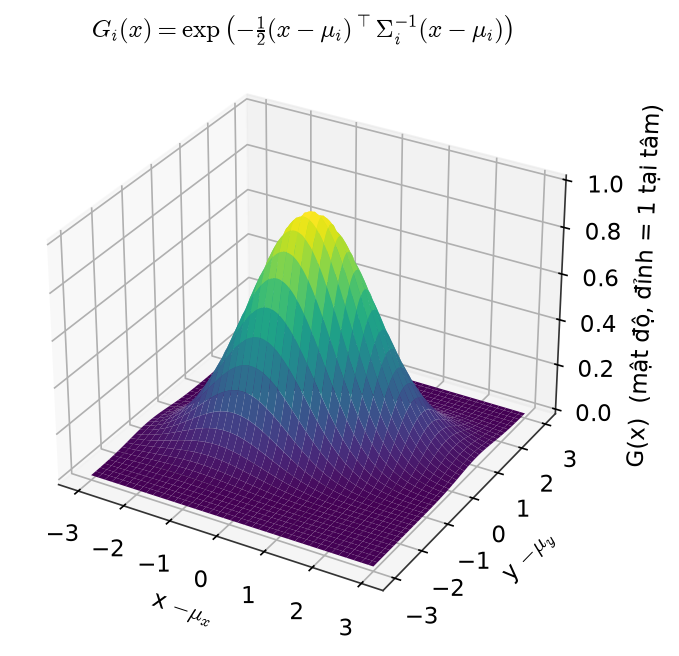
\includegraphics[width=0.95\linewidth]{ch2_gaussian_bump.png}
\captionof{figure}{\footnotesize Quả chuông mật độ Gaussian 3D}
\end{column}
\end{columns}
\end{frame}

% --- Slide 6 ---
\begin{frame}{Tham số hoá hiệp phương sai}
\begin{columns}
\begin{column}{0.55\textwidth}
\footnotesize
\begin{itemize}
    \item Không học trực tiếp $\Sigma$ để đảm bảo tính \textbf{positive semi-definite} trong lúc tối ưu.
    \item Thay vào đó học scale $s \in \mathbb{R}^3$ và quaternion xoay $q \in \mathbb{R}^4$:
    \[
    \Sigma = R S S^T R^T
    \]
    với $S = \mathrm{diag}(s)$, $R = R(q)$.
    \item Khởi tạo scale ban đầu dựa trên khoảng cách tới các điểm lân cận từ COLMAP.
\end{itemize}
\end{column}
\begin{column}{0.45\textwidth}
\centering
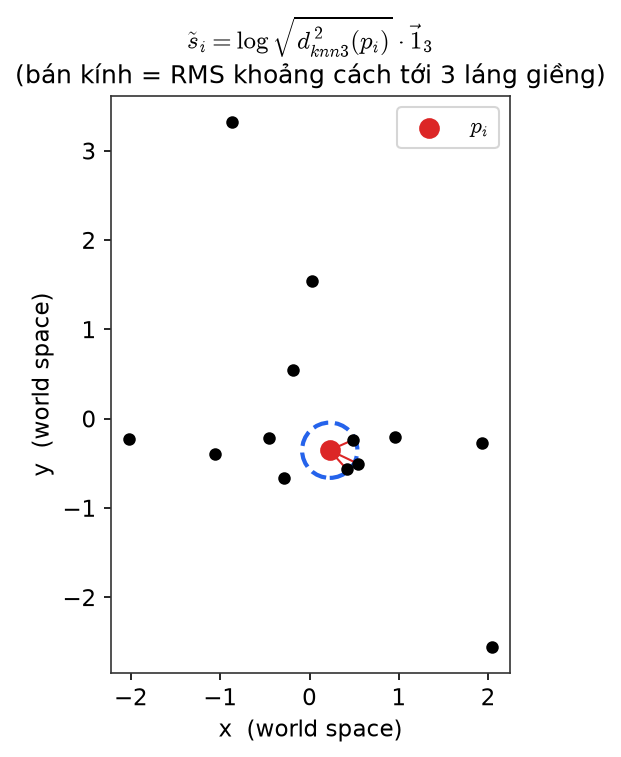
\includegraphics[width=0.78\linewidth]{ch1_scale_init.png}
\captionof{figure}{\footnotesize Khởi tạo scale từ khoảng cách lân cận}
\end{column}
\end{columns}
\end{frame}

% --- Slide 7 ---
\begin{frame}{Ellipsoid hiệp phương sai}
\begin{columns}
\begin{column}{0.55\textwidth}
\footnotesize
\begin{itemize}
    \item $\Sigma$ tương đương một \textbf{ellipsoid 3D} biểu diễn vùng ảnh hưởng của Gaussian.
    \item Trục ellipsoid = eigenvector của $\Sigma$.
    \item Độ dài trục = eigenvalue của $\Sigma$.
    \item Ellipsoid càng dẹt/kéo dài $\Rightarrow$ Gaussian càng bất đẳng hướng.
\end{itemize}
\end{column}
\begin{column}{0.45\textwidth}
\centering
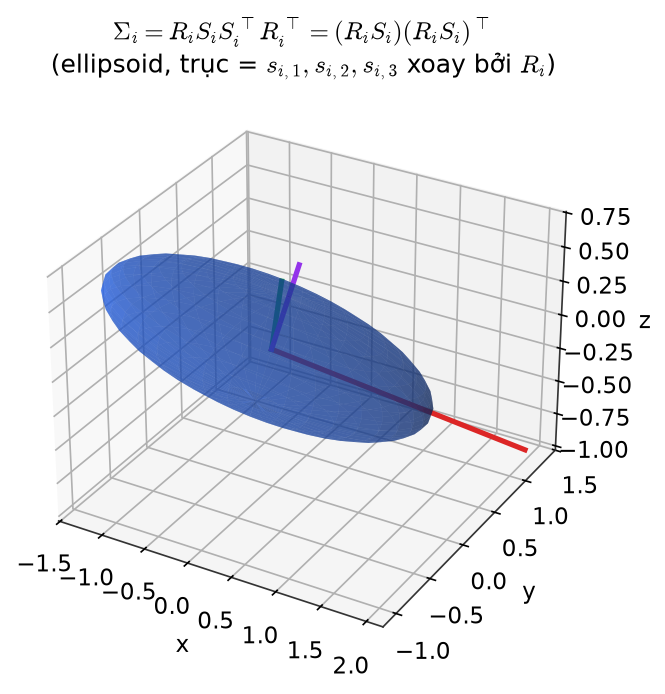
\includegraphics[width=0.95\linewidth]{ch2_covariance_ellipsoid.png}
\captionof{figure}{\footnotesize Ellipsoid ứng với $\Sigma$}
\end{column}
\end{columns}
\end{frame}

% --- Slide 8 ---
\begin{frame}{Màu sắc qua Spherical Harmonics (SH)}
\begin{columns}
\begin{column}{0.55\textwidth}
\footnotesize
\begin{itemize}
    \item Mỗi Gaussian không lưu 1 màu RGB cố định, mà lưu hệ số \textbf{SH}.
    \item Biểu diễn màu \textbf{phụ thuộc góc nhìn} (view-dependent), đặc tả hiệu ứng phản xạ/specular.
    \item Hệ số SH bậc 0 (DC) khởi tạo trực tiếp từ màu RGB quan sát được:
    \[
    f_{dc} = \mathrm{RGB2SH}(\text{color})
    \]
\end{itemize}
\end{column}
\begin{column}{0.45\textwidth}
\centering
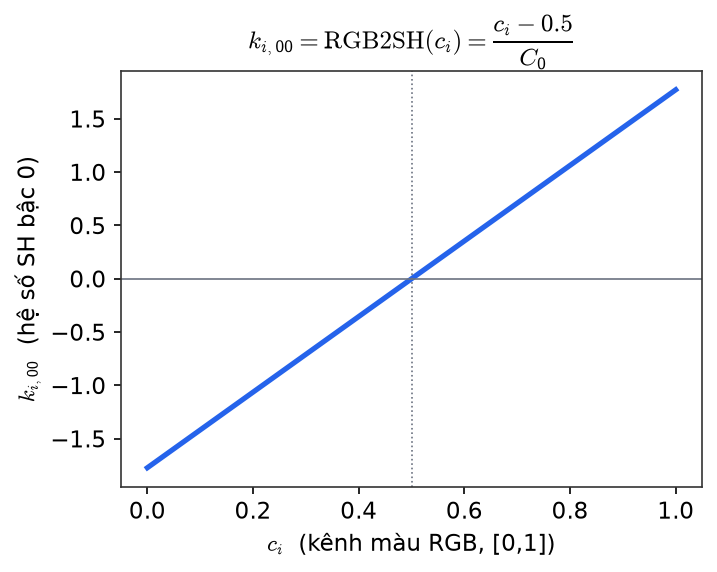
\includegraphics[width=0.95\linewidth]{ch1_rgb2sh.png}
\captionof{figure}{\footnotesize Chuyển đổi RGB $\to$ hệ số SH bậc 0}
\end{column}
\end{columns}
\end{frame}

% --- Slide 9 ---
\begin{frame}{Cơ sở SH và lịch tăng bậc}
\footnotesize
\begin{columns}
\begin{column}{0.5\textwidth}
\centering
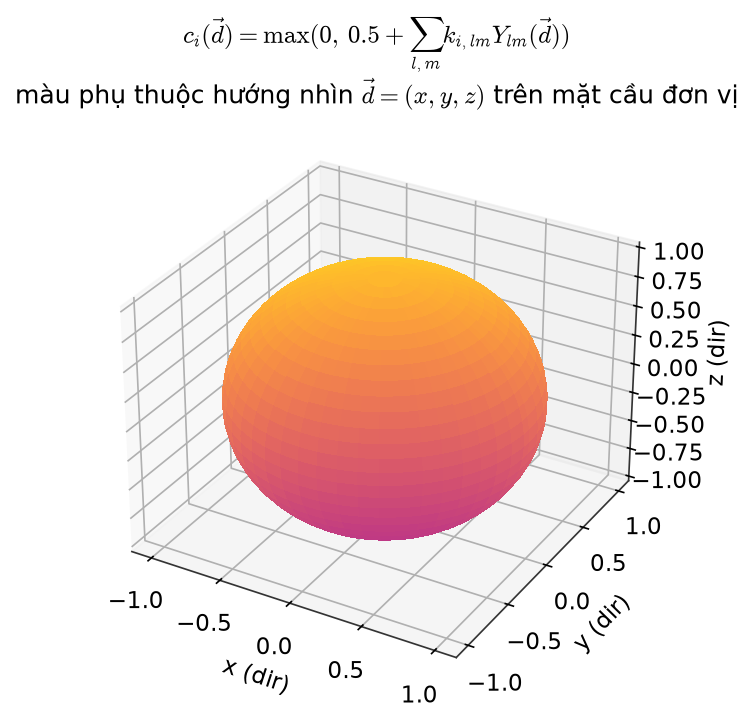
\includegraphics[width=0.9\linewidth]{ch2_sh_sphere.png}
\captionof{figure}{\footnotesize Các hàm cơ sở SH bậc thấp trên mặt cầu}
\end{column}
\begin{column}{0.5\textwidth}
\centering
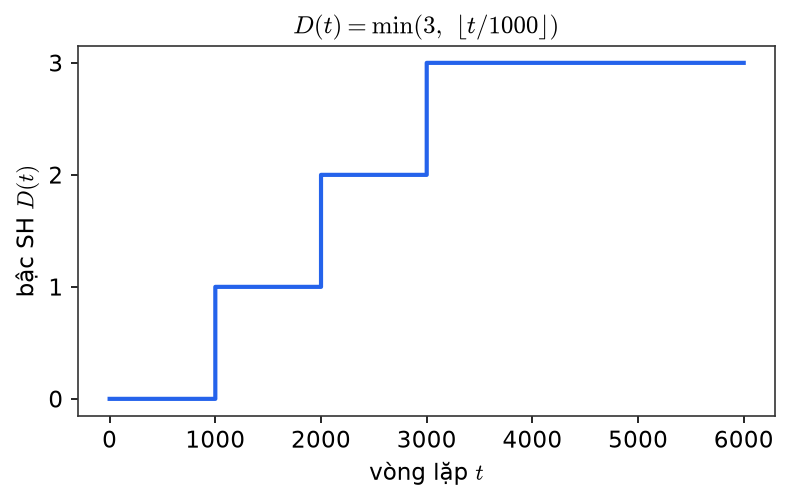
\includegraphics[width=0.9\linewidth]{ch2_sh_degree_schedule.png}
\captionof{figure}{\footnotesize Lịch tăng dần bậc SH khi huấn luyện}
\end{column}
\end{columns}
\vspace{0.2cm}
\small
Mỗi vài nghìn iteration tăng thêm 1 bậc SH, tối đa bậc 3 (16 hệ số/kênh màu).
\end{frame}

% --- Slide 10 ---
\begin{frame}{Khởi tạo từ SfM/COLMAP}
\begin{columns}
\begin{column}{0.55\textwidth}
\footnotesize
\begin{itemize}
    \item Gaussian ban đầu được khởi tạo tại các điểm \textbf{point-cloud thưa} do COLMAP tái tạo (Structure-from-Motion).
    \item \textbf{Scene extent}: đường chéo bounding box của các camera trong cảnh.
    \item Scene extent dùng làm tham chiếu cho ngưỡng phân tách Gaussian (\texttt{-{}-dense}) ở Adaptive Density Control (phần sau).
\end{itemize}
\end{column}
\begin{column}{0.45\textwidth}
\centering
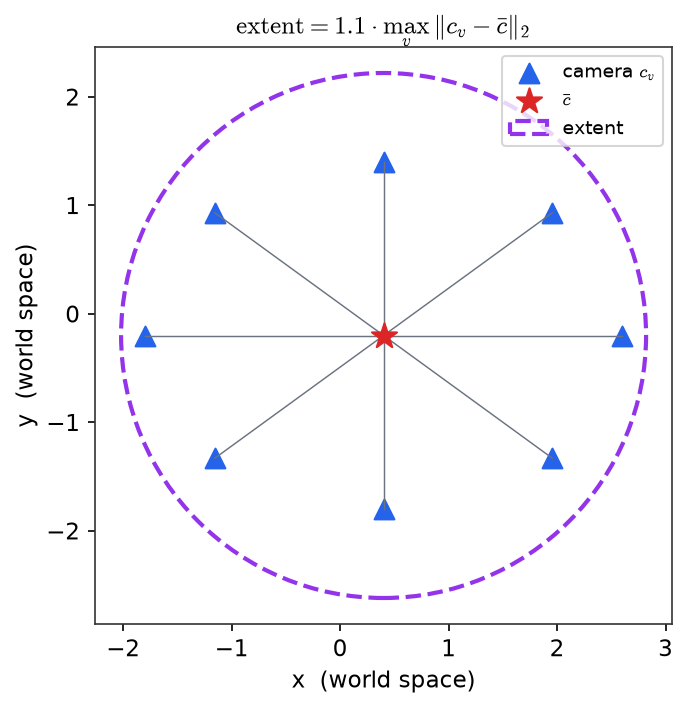
\includegraphics[width=0.95\linewidth]{ch1_extent.png}
\captionof{figure}{\footnotesize Scene extent từ bounding box camera}
\end{column}
\end{columns}
\end{frame}


% ===================== PHẦN SH =====================
\section{Nền tảng toán học đầy đủ: Spherical Harmonics}
% ============================================================
% Phần SH-A: Nền tảng toán học đầy đủ của Spherical Harmonics
% 9 slide, từ phương trình Laplace đến hàm điều hòa cầu thực
% File này KHÔNG tự đứng độc lập -- được \input trong main.tex
% ============================================================

% --- 1_1_laplace_equation.png ---
\begin{frame}{Xuất phát điểm: Phương trình Laplace}
\begin{columns}[T]
\begin{column}{0.52\textwidth}
\footnotesize
\begin{itemize}
    \item Hàm điều hòa (harmonic function) $\Phi(x,y,z)$ là nghiệm của phương trình Laplace trong không gian 3 chiều:
    $$\nabla^2\Phi=\frac{\partial^2\Phi}{\partial x^2}+\frac{\partial^2\Phi}{\partial y^2}+\frac{\partial^2\Phi}{\partial z^2}=0$$
    \item Chuyển sang toạ độ cầu $(r,\theta,\phi)$ với $x=r\sin\theta\cos\phi,\ y=r\sin\theta\sin\phi,\ z=r\cos\theta$, toán tử Laplace trở thành:
    $$\nabla^2\Phi=\dfrac{1}{r^2}\dfrac{\partial}{\partial r}\!\left(r^2\dfrac{\partial\Phi}{\partial r}\right)+\dfrac{1}{r^2\sin\theta}\dfrac{\partial}{\partial\theta}\!\left(\sin\theta\dfrac{\partial\Phi}{\partial\theta}\right)+\dfrac{1}{r^2\sin^2\theta}\dfrac{\partial^2\Phi}{\partial\phi^2}=0$$
    \item Phần góc $(\theta,\phi)$ của nghiệm chính là hàm điều hòa cầu $Y_l^m$ -- lý do SH là ``cơ sở tự nhiên'' cho hàm số trên mặt cầu, tương tự chuỗi Fourier là cơ sở tự nhiên trên đường tròn.
    \item Kiểm chứng số học (sai phân hữu hạn) trên lưới 2D lát cắt $z=\text{const}$: $\Phi=x^2-y^2$ cho $\nabla^2\Phi\approx0$, trong khi $\Phi=x^2+y^2$ cho $\nabla^2\Phi=4\neq0$.
    \item Đây là điểm khởi đầu của toàn bộ chuỗi suy diễn: Laplace $\to$ tách biến $\to$ Legendre $\to$ $Y_l^m$.
\end{itemize}
\end{column}
\begin{column}{0.44\textwidth}
\centering
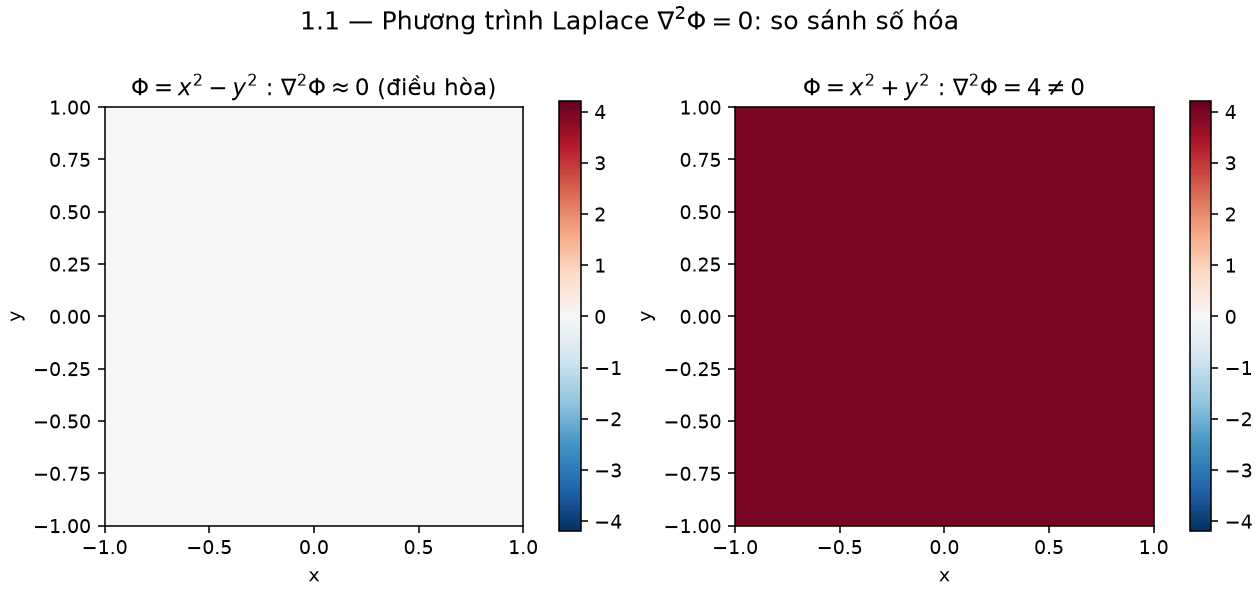
\includegraphics[width=0.9\linewidth]{1_1_laplace_equation.png}
\captionof{figure}{\footnotesize Kiểm chứng số học $\nabla^2\Phi=0$ (hàm điều hòa) so với $\nabla^2\Phi\neq0$ trên lưới 2D.}
\end{column}
\end{columns}
\end{frame}

% --- 1_2_spherical_coords.png ---
\begin{frame}{Hệ toạ độ cầu $(\theta,\phi)$}
\begin{columns}[T]
\begin{column}{0.52\textwidth}
\begin{itemize}
    \item Toạ độ cầu dùng góc thiên đỉnh (polar angle) $\theta\in[0,\pi]$ và góc phương vị (azimuthal angle) $\phi\in[0,2\pi)$.
    \item Quan hệ với toạ độ Descartes trên mặt cầu bán kính $r$:
    $$
    \begin{aligned}
    x&=r\sin\theta\cos\phi\\
    y&=r\sin\theta\sin\phi\\
    z&=r\cos\theta
    \end{aligned}
    $$
    \item Với mặt cầu đơn vị ($r=1$): $(x,y,z)=(\sin\theta\cos\phi,\ \sin\theta\sin\phi,\ \cos\theta)$.
    \item Các hệ số $\sin\theta,\ \cos\theta,\ \sin^2\theta$ xuất hiện trực tiếp trong toán tử Laplace cầu -- đây là nguồn gốc của trọng số đo (measure) $d\Omega=\sin\theta\,d\theta\,d\phi$ dùng trong tích phân trực chuẩn về sau.
    \item Lưới toạ độ cầu $(\theta,\phi)$ được dựng bằng \texttt{meshgrid} và chiếu lên mặt cầu đơn vị để trực quan hoá.
\end{itemize}
\end{column}
\begin{column}{0.44\textwidth}
\centering
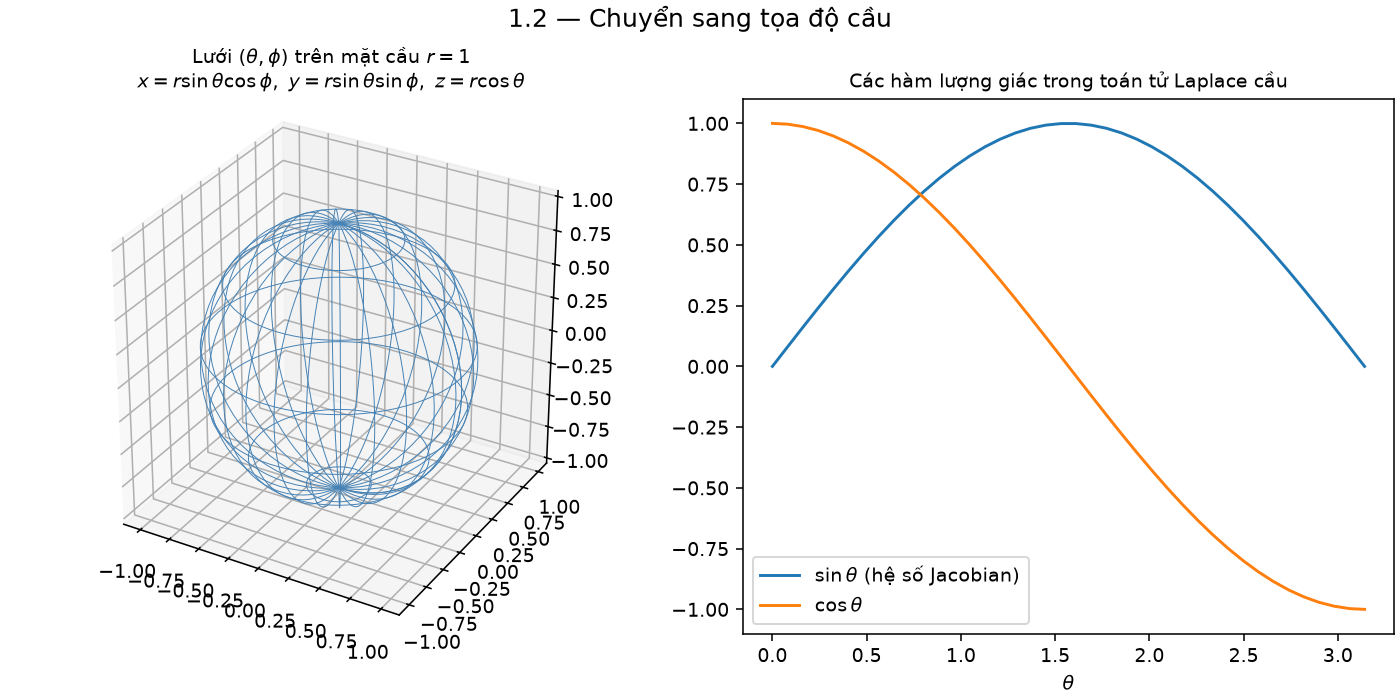
\includegraphics[width=0.9\linewidth]{1_2_spherical_coords.png}
\captionof{figure}{\footnotesize Lưới toạ độ cầu $(\theta,\phi)$ trên mặt cầu đơn vị.}
\end{column}
\end{columns}
\end{frame}

% --- 1_2b_radial_solution.png ---
\begin{frame}{Tách biến: Nghiệm phần bán kính $R(r)$}
\begin{columns}[T]
\begin{column}{0.52\textwidth}
\footnotesize
\begin{itemize}
    \item Giả sử nghiệm tách được: $\Phi(r,\theta,\phi)=R(r)\,\Theta(\theta)\,\Phi_m(\phi)$. Nhân hai vế phương trình Laplace với $r^2/(R\Theta\Phi_m)$, ta tách thành phần chỉ phụ thuộc $r$ và phần chỉ phụ thuộc $(\theta,\phi)$:
    $$\underbrace{\frac{1}{R}\frac{d}{dr}\!\left(r^2\frac{dR}{dr}\right)}_{\text{chỉ phụ thuộc }r}+\underbrace{\frac{1}{\Theta\sin\theta}\frac{d}{d\theta}\!\left(\sin\theta\frac{d\Theta}{d\theta}\right)+\frac{1}{\Phi_m\sin^2\theta}\frac{d^2\Phi_m}{d\phi^2}}_{\text{chỉ phụ thuộc }\theta,\phi}=0$$
    \item Vì hai nhóm phụ thuộc biến độc lập nhau, mỗi nhóm phải bằng một hằng số đối nhau. Đặt hằng số phân ly là $l(l+1)$:
    $$\frac{d}{dr}\!\left(r^2\frac{dR}{dr}\right)=l(l+1)R$$
    \item Nghiệm tổng quát của phương trình Euler-Cauchy này là hai nhánh độc lập:
    $$R(r)=A\,r^{l}+\dfrac{B}{r^{l+1}}$$
    \item Nhánh $r^l$ hữu hạn tại gốc toạ độ $r=0$; nhánh $r^{-l-1}$ hữu hạn tại vô cực -- tuỳ điều kiện biên vật lý mà chọn nhánh phù hợp.
\end{itemize}
\end{column}
\begin{column}{0.44\textwidth}
\centering
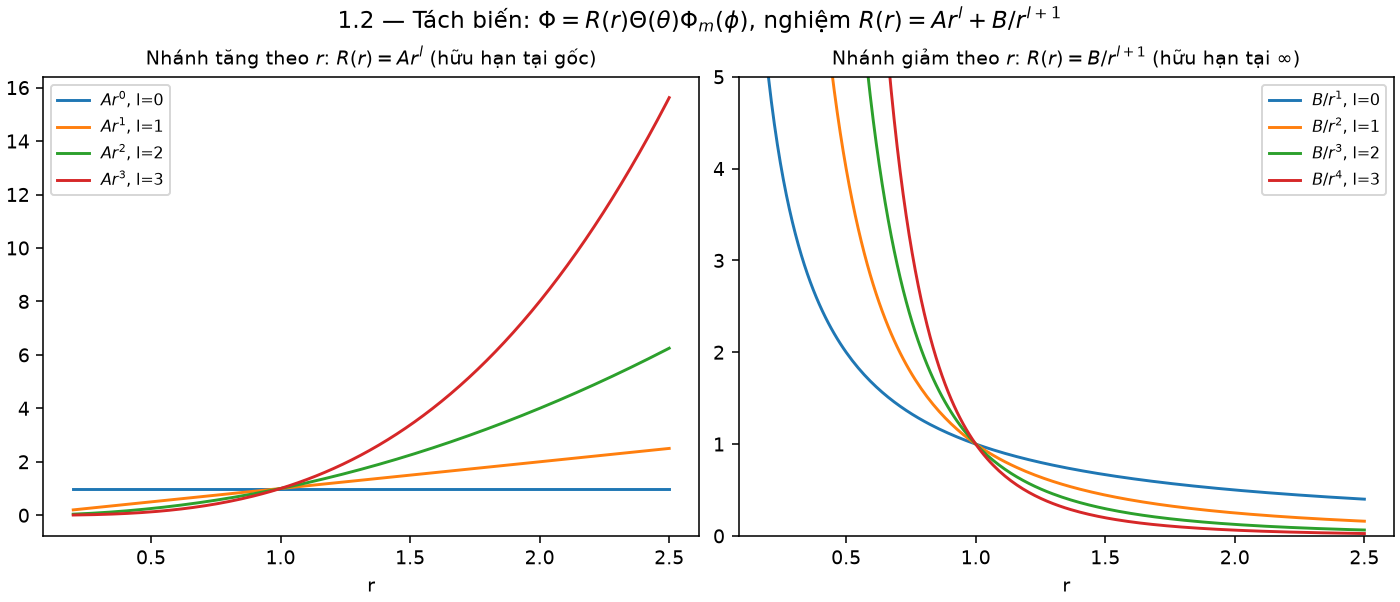
\includegraphics[width=0.9\linewidth]{1_2b_radial_solution.png}
\captionof{figure}{\footnotesize Hai nhánh nghiệm bán kính $R(r)=Ar^l$ và $R(r)=B/r^{l+1}$ với $l=0,1,2,3$.}
\end{column}
\end{columns}
\end{frame}

% --- 1_3_azimuthal_solution.png ---
\begin{frame}{Tách biến: Nghiệm phần phương vị $\Phi_m(\phi)$}
\begin{columns}[T]
\begin{column}{0.52\textwidth}
\begin{itemize}
    \item Từ phần góc còn lại, đặt hằng số tách thứ hai:
    $$-\dfrac{1}{\Phi_m}\dfrac{d^2\Phi_m}{d\phi^2}=m^2$$
    \item Phương trình vi phân thu được: $\dfrac{d^2\Phi_m}{d\phi^2}=-m^2\Phi_m$, có nghiệm tổng quát dạng sóng phức:
    $$\Phi_m(\phi)=e^{im\phi}$$
    \item Điều kiện tuần hoàn vật lý bắt buộc $\Phi_m(\phi+2\pi)=\Phi_m(\phi)$, tức $e^{im\cdot2\pi}=1$, dẫn đến điều kiện lượng tử hoá:
    $$m\in\mathbb{Z}$$
    \item Phần thực $\cos(m\phi)$ và quỹ đạo phức $e^{im\phi}=\cos(m\phi)+i\sin(m\phi)$ trên vòng tròn đơn vị được minh hoạ cho các giá trị nguyên $m=0,1,2,3$.
    \item Đây chính là "phiên bản cầu" của chuỗi Fourier theo góc phương vị -- bước trung gian trước khi ghép với nghiệm Legendre theo $\theta$.
\end{itemize}
\end{column}
\begin{column}{0.44\textwidth}
\centering
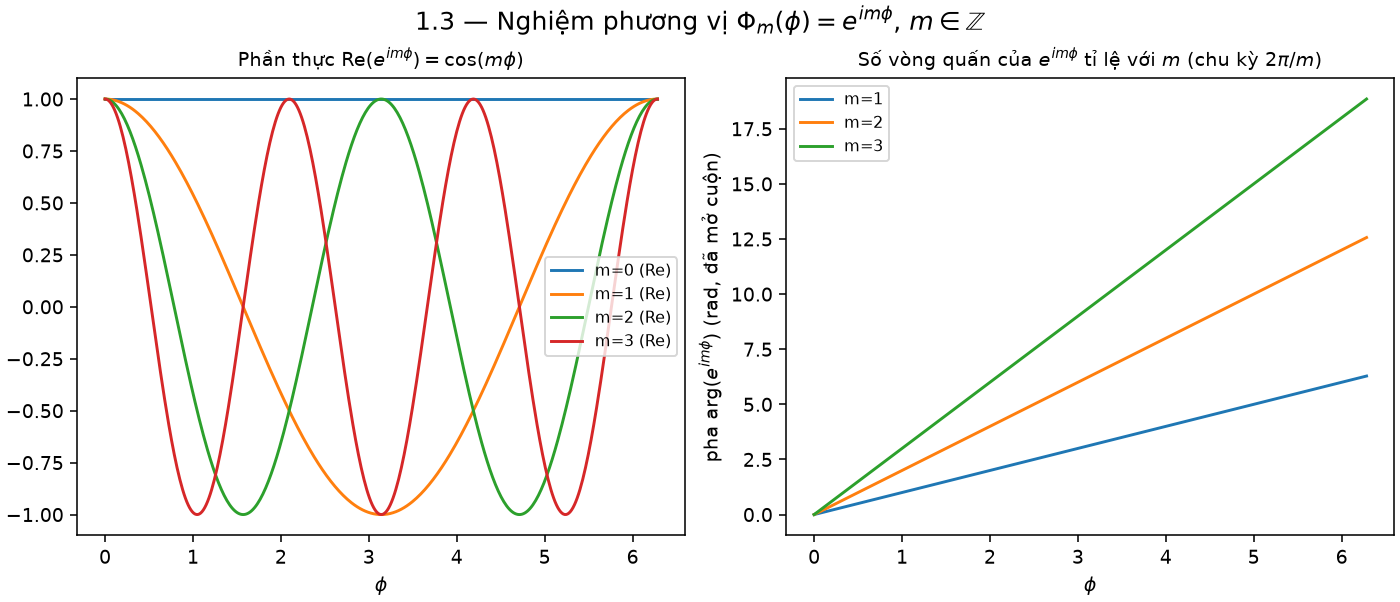
\includegraphics[width=0.9\linewidth]{1_3_azimuthal_solution.png}
\captionof{figure}{\footnotesize $\cos(m\phi)$ và quỹ đạo $e^{im\phi}$ trên vòng tròn đơn vị, $m=0,1,2,3$.}
\end{column}
\end{columns}
\end{frame}

% --- 1_4_legendre_functions.png ---
\begin{frame}{Phương trình Legendre liên kết}
\begin{columns}[T]
\begin{column}{0.52\textwidth}
\footnotesize
\begin{itemize}
    \item Đặt $x=\cos\theta$, phần góc $\theta$ còn lại trở thành \textbf{phương trình Legendre liên kết} (associated Legendre equation):
    $$\frac{d}{dx}\!\left[(1-x^2)\frac{d\Theta}{dx}\right]+\left[l(l+1)-\frac{m^2}{1-x^2}\right]\Theta=0$$
    \item Nghiệm hữu hạn tại hai cực $x=\pm1$ (cực Bắc/Nam của mặt cầu) chỉ tồn tại khi $l=0,1,2,\dots$ và $m=-l,\dots,l$ nguyên -- đây chính là nguồn gốc của điều kiện lượng tử hoá bậc $l$.
    \item Nghiệm là \textbf{hàm Legendre liên kết}:
    $$P_l^m(x)=(-1)^m(1-x^2)^{m/2}\frac{d^m}{dx^m}P_l(x)$$
    với đa thức Legendre thường (trường hợp $m=0$) cho bởi công thức Rodrigues:
    $$P_l(x)=\frac{1}{2^l\,l!}\frac{d^l}{dx^l}(x^2-1)^l$$
    \item Đồ thị minh hoạ: đa thức Legendre $P_l(x)$ với $l=0,\dots,5$, và hàm Legendre liên kết $P_3^m(x)$ với $m=0,\dots,3$.
\end{itemize}
\end{column}
\begin{column}{0.44\textwidth}
\centering
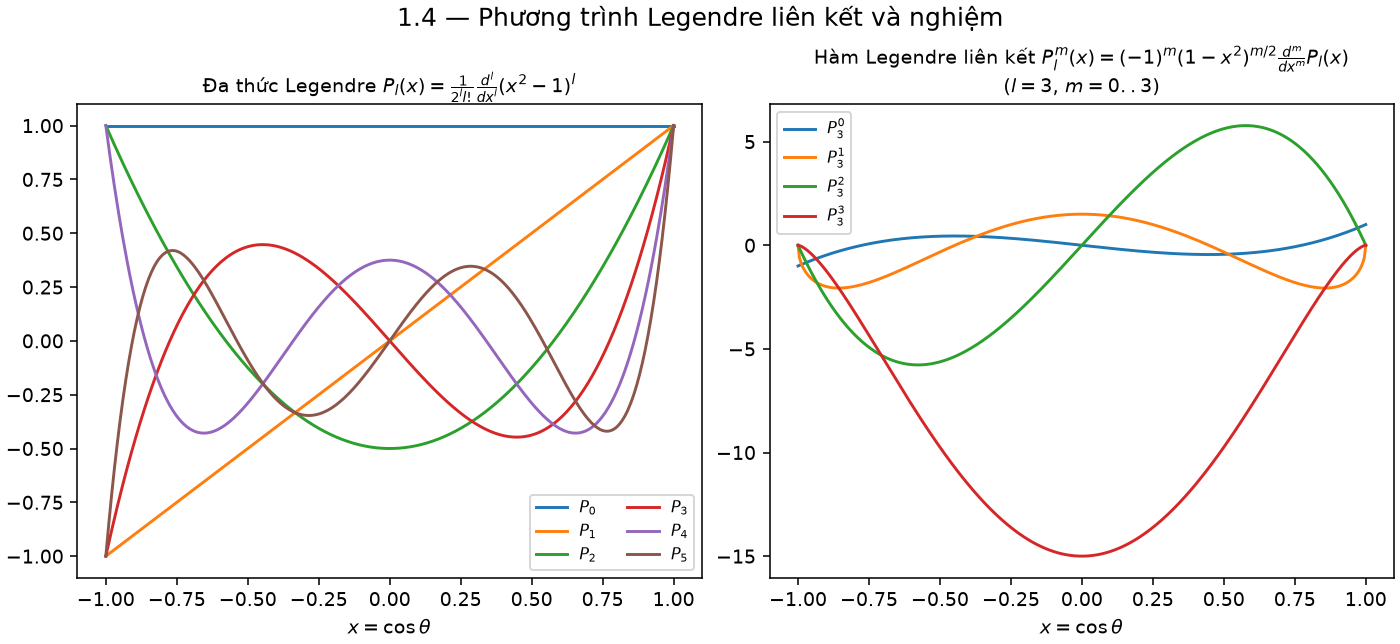
\includegraphics[width=0.9\linewidth]{1_4_legendre_functions.png}
\captionof{figure}{\footnotesize $P_l(x)$ với $l=0..5$ và $P_3^m(x)$ với $m=0..3$.}
\end{column}
\end{columns}
\end{frame}

% --- 1_5_spherical_harmonics_lobes.png ---
\begin{frame}{Ghép lại: Định nghĩa đầy đủ $Y_l^m$}
\begin{columns}[T]
\begin{column}{0.52\textwidth}
\footnotesize
\begin{itemize}
    \item Ghép nghiệm phần Legendre $P_l^m(\cos\theta)$ với nghiệm phương vị $e^{im\phi}$, cùng hằng số chuẩn hoá để đảm bảo trực chuẩn, ta có định nghĩa đầy đủ của hàm điều hòa cầu (spherical harmonics):
    $$\boxed{Y_l^m(\theta,\phi)=\sqrt{\dfrac{2l+1}{4\pi}\dfrac{(l-m)!}{(l+m)!}}\;P_l^m(\cos\theta)\,e^{im\phi}}$$
    \item $l\ge0$ gọi là \textbf{bậc} (degree), $m\in\{-l,\dots,l\}$ gọi là \textbf{bậc con} (order) -- ứng với mỗi $l$ có $2l+1$ hàm $Y_l^m$ độc lập.
    \item Hình dạng "thuỳ" (lobe) của $|Y_l^m|$ trên mặt cầu phụ thuộc vào cặp $(l,m)$: $l$ càng lớn, số thuỳ càng nhiều (dao động không gian càng nhanh); $m$ quyết định phân bố thuỳ theo phương vị.
    \item Trực quan hoá: bán kính tại mỗi hướng $=|Y_l^m(\theta,\phi)|$, màu sắc thể hiện dấu/giá trị của phần thực $\mathrm{Re}(Y_l^m)$.
\end{itemize}
\end{column}
\begin{column}{0.44\textwidth}
\centering
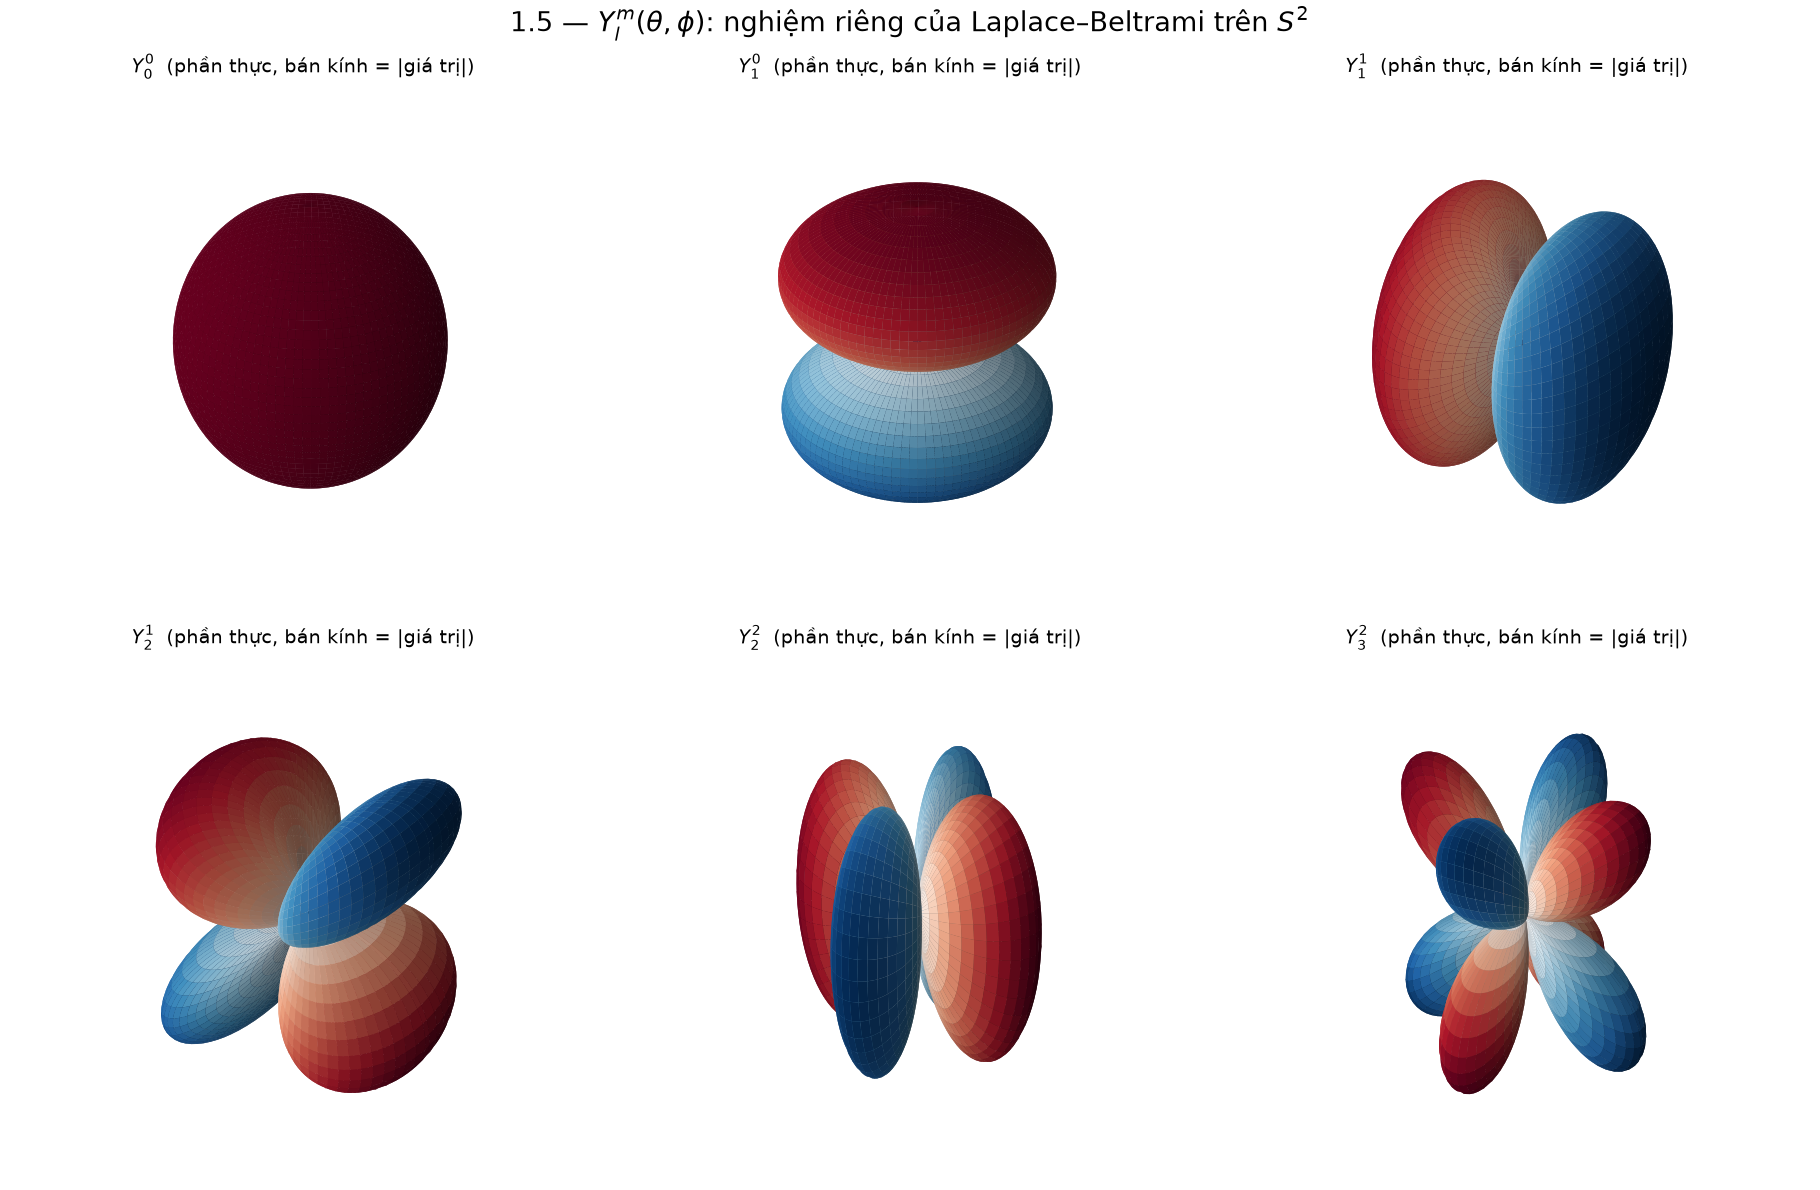
\includegraphics[width=0.9\linewidth]{1_5_spherical_harmonics_lobes.png}
\captionof{figure}{\footnotesize Hình dạng thuỳ của $\mathrm{Re}(Y_l^m)$ trên mặt cầu cho các cặp $(l,m)$ tiêu biểu.}
\end{column}
\end{columns}
\end{frame}

% --- 1_6_eigenvalue_check.png ---
\begin{frame}{$Y_l^m$ là hàm riêng của Laplace-Beltrami}
\begin{columns}[T]
\begin{column}{0.52\textwidth}
\begin{itemize}
    \item Hàm điều hòa cầu $Y_l^m$ chính là \textbf{hàm riêng} (eigenfunction) của toán tử Laplace-Beltrami $\nabla^2_{S^2}$ trên mặt cầu đơn vị $S^2$ (phần góc của toán tử Laplace 3D), với \textbf{trị riêng} (eigenvalue) $-l(l+1)$:
    $$\nabla^2_{S^2}Y_l^m=-l(l+1)\,Y_l^m$$
    \item Đây là hệ quả trực tiếp của quá trình tách biến: $l(l+1)$ chính là hằng số phân ly đã đặt ra ở bước tách phương trình Laplace 3D thành phần bán kính và phần góc.
    \item Kiểm chứng số học bằng sai phân hữu hạn của $\nabla^2_{S^2}$ trên lưới $(\theta,\phi)$:
    $$\nabla^2_{S^2}Y=\frac{1}{\sin\theta}\frac{\partial}{\partial\theta}\!\left(\sin\theta\frac{\partial Y}{\partial\theta}\right)+\frac{1}{\sin^2\theta}\frac{\partial^2Y}{\partial\phi^2}$$
    tính bằng \texttt{np.gradient} hai lần, sau đó so sánh tỉ số $\nabla^2_{S^2}Y/Y$ với giá trị lý thuyết $-l(l+1)$.
    \item Kết quả số khớp với lý thuyết trong sai số rời rạc hoá -- xác nhận $Y_l^m$ đúng là nghiệm riêng, không phải xấp xỉ.
\end{itemize}
\end{column}
\begin{column}{0.44\textwidth}
\centering
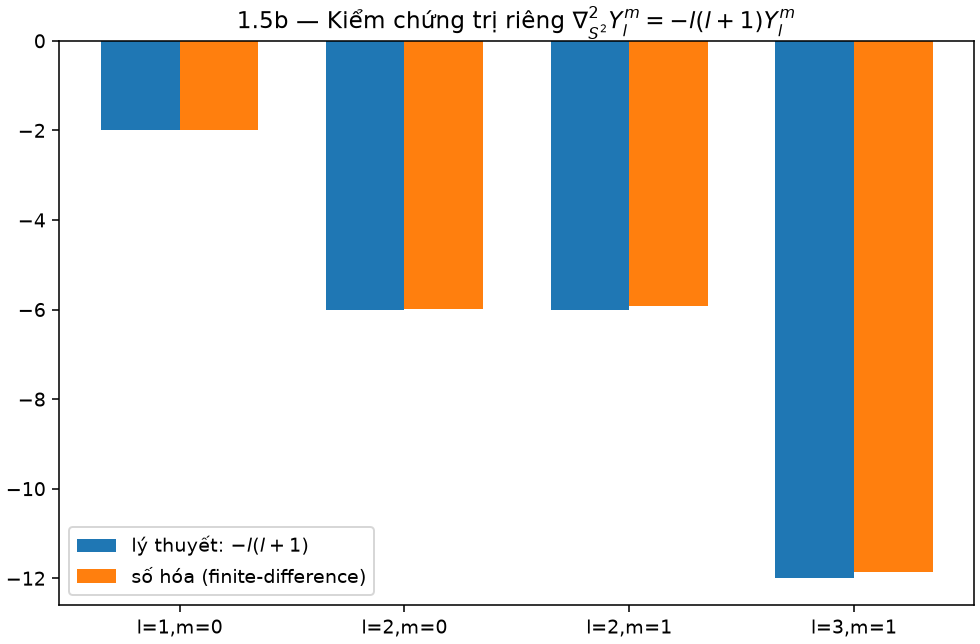
\includegraphics[width=0.9\linewidth]{1_6_eigenvalue_check.png}
\captionof{figure}{\footnotesize Kiểm chứng số học trị riêng $-l(l+1)$ bằng sai phân hữu hạn của $\nabla^2_{S^2}Y_l^m$.}
\end{column}
\end{columns}
\end{frame}

% --- 1_7_orthonormality_matrix.png ---
\begin{frame}{Tính trực chuẩn của hệ $\{Y_l^m\}$}
\begin{columns}[T]
\begin{column}{0.52\textwidth}
\scriptsize
\begin{itemize}
    \item Hệ $\{Y_l^m\}$ thoả \textbf{trực chuẩn} trên $S^2$ với đo $d\Omega{=}\sin\theta\,d\theta\,d\phi$:
    $\int_{S^2}Y_l^m(Y_{l'}^{m'})^{*}d\Omega{=}\delta_{ll'}\delta_{mm'}$.
    \item Hệ quả Sturm-Liouville (phương trình Legendre, phần $\theta$) kết hợp trực giao $e^{im\phi}$ trên chu kỳ $2\pi$ (phần $\phi$).
    \item Kiểm chứng số: ma trận Gram $M_{ij}{=}\sum Y_i(Y_j)^{*}\sin\theta\,\Delta\theta\Delta\phi \approx \delta_{ij}$ cho $l{=}0,1,2$.
    \item Nền tảng dùng $\{Y_l^m\}$ làm cơ sở Fourier trên mặt cầu — hệ số tính bằng phép chiếu, không chồng lấn giữa các bậc.
\end{itemize}
\end{column}
\begin{column}{0.44\textwidth}
\centering
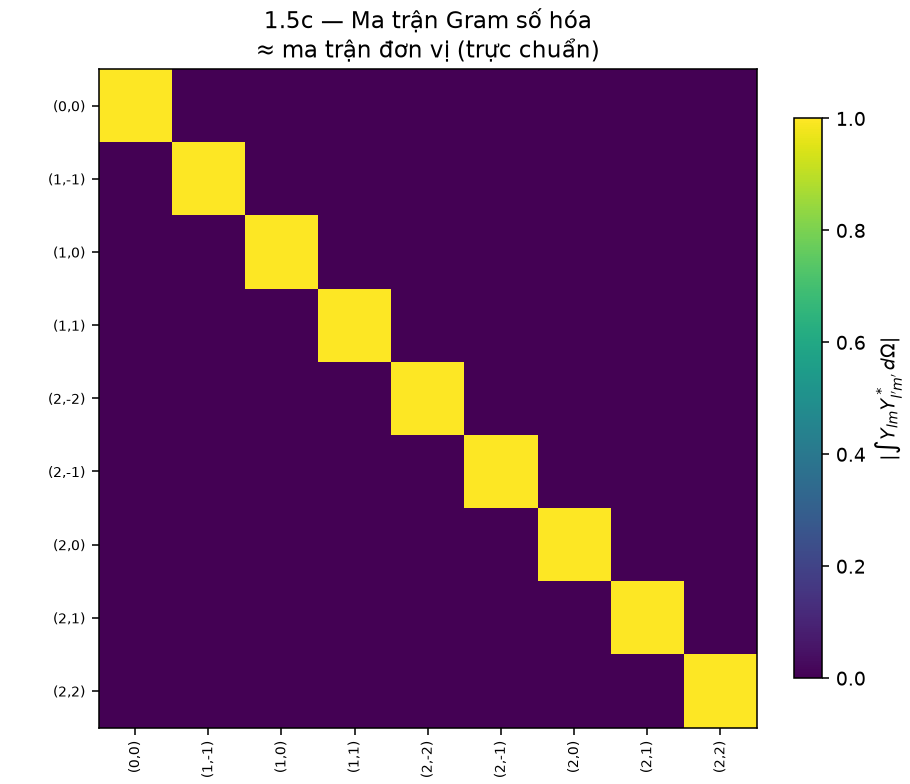
\includegraphics[width=0.9\linewidth]{1_7_orthonormality_matrix.png}
\captionof{figure}{\footnotesize Ma trận Gram xấp xỉ ma trận đơn vị.}
\end{column}
\end{columns}
\end{frame}

% --- 2_1_real_sh_construction.png ---
\begin{frame}{Từ SH phức sang SH thực (Real SH)}
\begin{columns}[T]
\begin{column}{0.55\textwidth}
\scriptsize
    Đồ hoạ máy tính (3DGS) dùng số thực, nhưng $Y_l^m$ gốc chứa $e^{im\phi}$ là số phức $\Rightarrow$ tổ hợp tuyến tính $Y_l^{\pm m}$ để có cơ sở \textbf{thực} tương đương, giữ trực chuẩn:
    \[
    Y_{lm}^{\text{real}}=
    \begin{cases}
    \frac{i}{\sqrt{2}}\left(Y_l^{m}-(-1)^m Y_l^{-m}\right) & m<0\\
    Y_l^0 & m=0\\
    \frac{1}{\sqrt{2}}\left(Y_l^{-m}+(-1)^m Y_l^{m}\right) & m>0
    \end{cases}
    \]
    \begin{itemize}
    \item Với $m\neq0$: tổ hợp $Y_l^m$ và liên hợp $Y_l^{-m}=(-1)^m(Y_l^m)^*$ triệt tiêu phần ảo.
    \item \textbf{Lý do dùng SH thực trong 3DGS}: tránh số phức toàn pipeline, giảm nửa số biến lưu, khớp trực tiếp RGB trong \texttt{computeColorFromSH}.
    \end{itemize}
\end{column}
\begin{column}{0.45\textwidth}
\centering
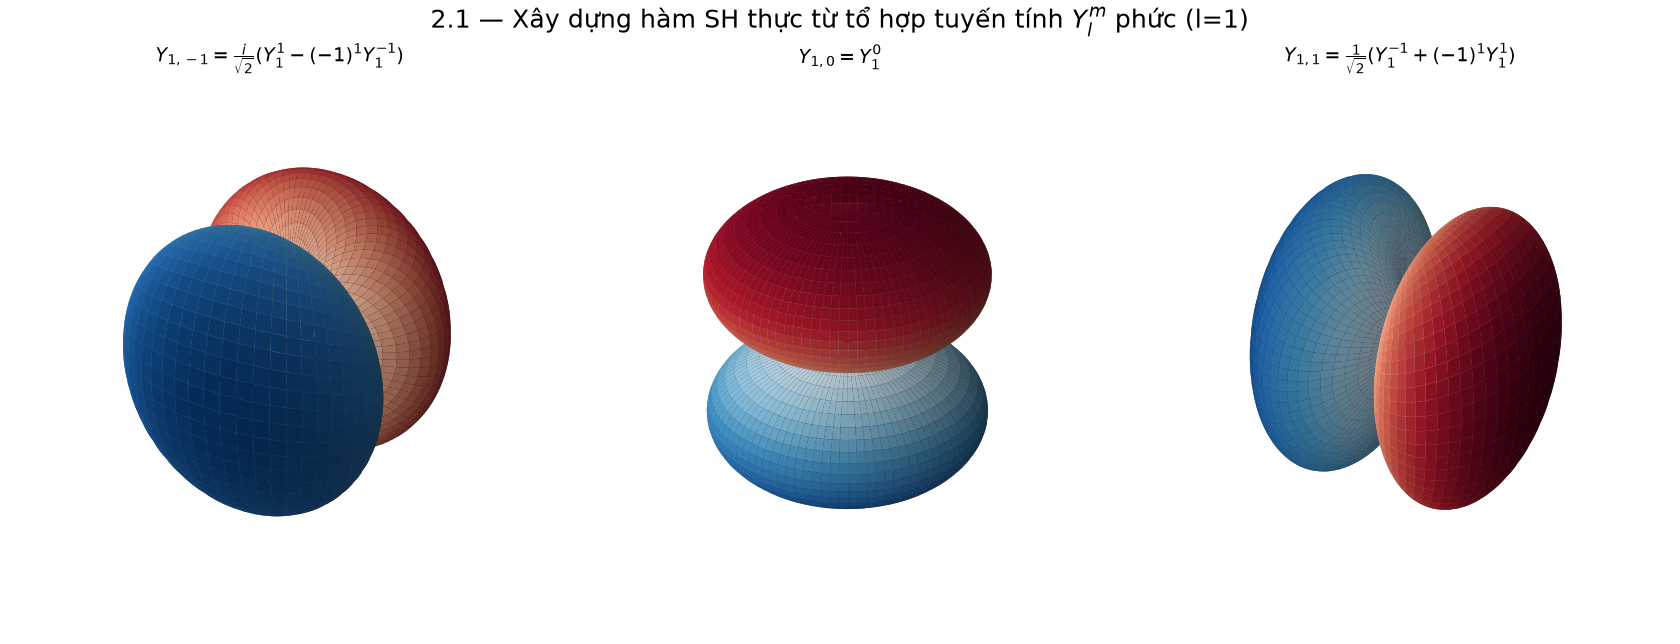
\includegraphics[width=0.95\linewidth]{2_1_real_sh_construction.png}
\captionof{figure}{\footnotesize Dựng $Y_{1,m}^{\text{real}}$, $m{=}-1,0,1$.}
\end{column}
\end{columns}
\end{frame}

% partSH_B.tex --- SH-B: Ứng dụng SH vào 3DGS (phần toán chuyên sâu)
% KHÔNG chứa \documentclass / \usepackage / \begin{document}

% --- 2_2_low_order_real_sh.png ---
\begin{frame}{Real SH bậc thấp: $Y_{00}, Y_{1,-1}, Y_{10}, Y_{11}$}
\begin{columns}[T]
\begin{column}{0.52\linewidth}
\footnotesize
\begin{itemize}
    \item Đặt $x=\sin\theta\cos\phi,\ y=\sin\theta\sin\phi,\ z=\cos\theta$ trên mặt cầu đơn vị.
    \item Bậc $l=0$ (hằng số, không phụ thuộc hướng):
    $$Y_{00}=C_0=\frac12\sqrt{\frac1\pi}$$
    \item Bậc $l=1$ (3 hàm tuyến tính theo $x,y,z$), với $C_1=\frac12\sqrt{\frac3\pi}$:
    $$Y_{1,-1}=C_1\,y,\quad Y_{1,0}=C_1\,z,\quad Y_{1,1}=C_1\,x$$
    \item Bậc $l=2$: 5 hàm bậc 2 theo $x,y,z$ (vd. $xy,\ yz,\ 3z^2-1,\ xz,\ x^2-y^2$), mỗi hàm nhân một hằng số chuẩn hoá $C_2^{(m)}$.
    \item Trong 3DGS, các hằng số $C_0,C_1,\dots$ này là \emph{cố định}; các hệ số nhân $k_{lm}$ (tương ứng \texttt{f\_dc} cho $l=0$ và \texttt{f\_rest} cho $l\ge1$) mới là tham số \textbf{học được} lưu trong mỗi Gaussian.
\end{itemize}
\end{column}
\begin{column}{0.46\linewidth}
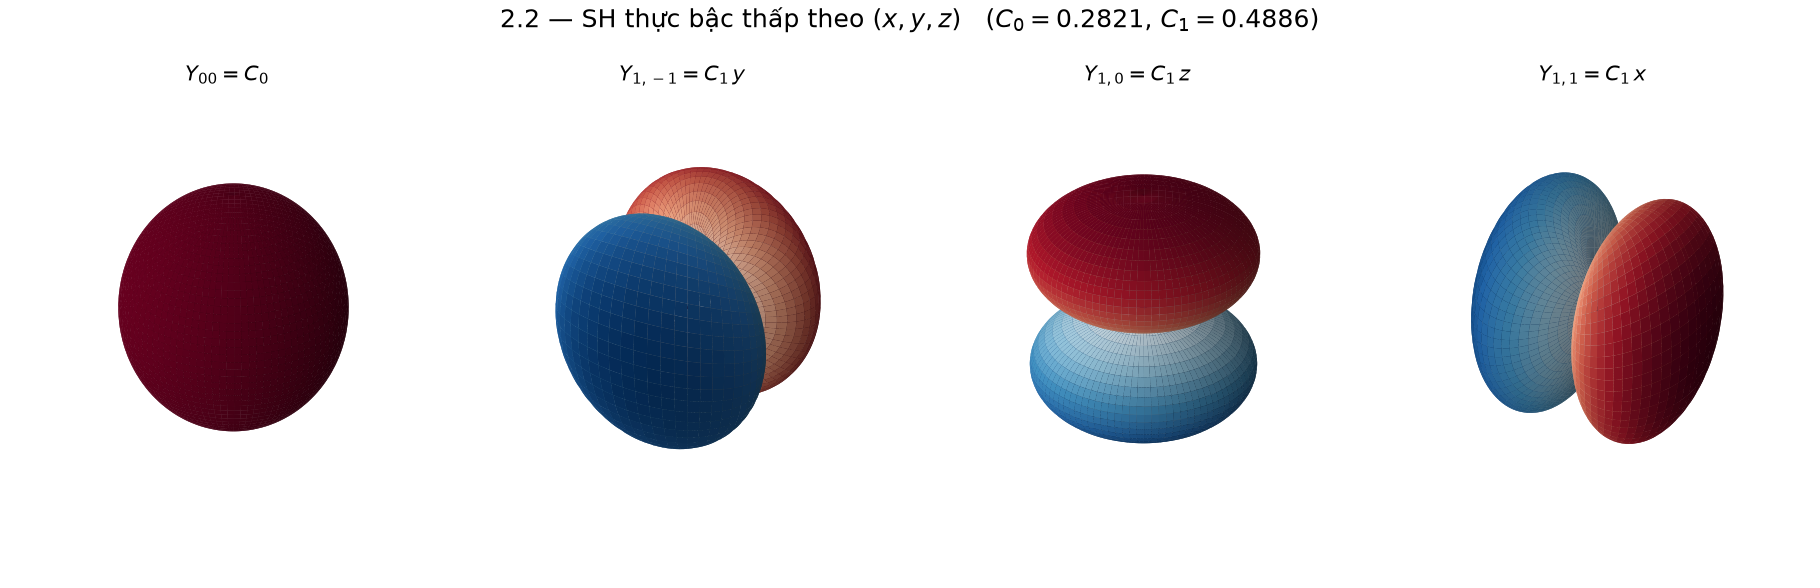
\includegraphics[width=0.9\linewidth]{2_2_low_order_real_sh.png}
\captionof{figure}{\footnotesize Bốn hàm SH thực bậc thấp $Y_{00}=C_0$, $Y_{1,-1}=C_1y$, $Y_{1,0}=C_1z$, $Y_{1,1}=C_1x$ vẽ trên mặt cầu (bán kính $=|$giá trị$|$).}
\end{column}
\end{columns}
\end{frame}

% --- 3_1_fourier_vs_sh.png ---
\begin{frame}{Chuỗi Fourier (1D) so với khai triển SH (2D cầu)}
\begin{columns}[T]
\begin{column}{0.52\linewidth}
\footnotesize
\begin{itemize}
    \item Fourier 1D là cơ sở trực chuẩn cho hàm tuần hoàn trên đường tròn $S^1$:
    $$f(\phi)=\sum_{n=-\infty}^{\infty} c_n\,e^{in\phi}$$
    \item SH là cơ sở trực chuẩn cho hàm trên mặt cầu $S^2$:
    $$f(\theta,\phi)=\sum_{l=0}^{\infty}\sum_{m=-l}^{l} k_{lm}\,Y_{lm}(\theta,\phi)$$
    \item Cùng một ý tưởng: phân tích tín hiệu theo \emph{tần số không gian} tăng dần ($n$ hoặc $l$ càng lớn thì dao động càng nhanh), chỉ khác miền định nghĩa (đường tròn 1D vs. mặt cầu 2D).
    \item Cả hai đều dựa trên tính \textbf{đầy đủ} (completeness) và \textbf{trực chuẩn} của hệ hàm cơ sở, cho phép biểu diễn chính xác mọi hàm bình phương khả tích khi lấy tổng vô hạn.
    \item Trong 3DGS, $f$ chính là hàm màu $c_i(\vec d)$ theo hướng nhìn $\vec d\in S^2$.
\end{itemize}
\end{column}
\begin{column}{0.46\linewidth}
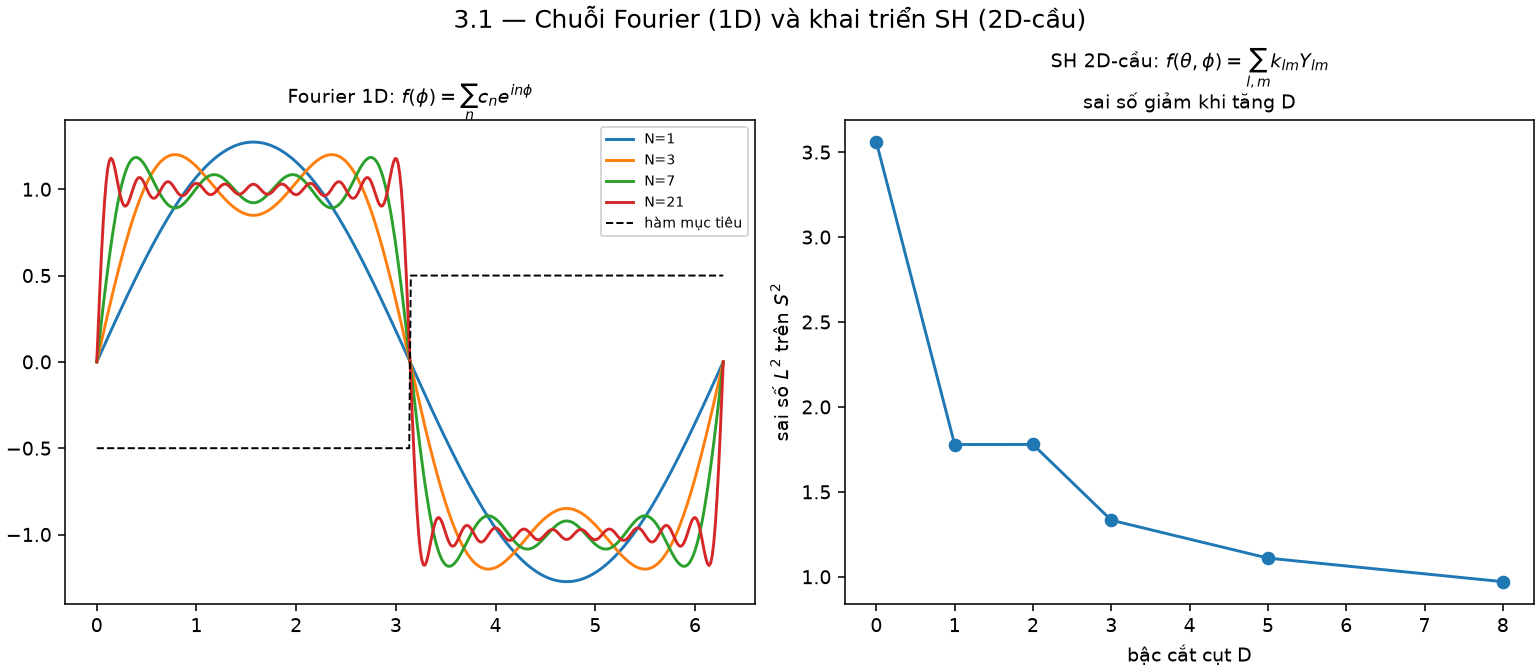
\includegraphics[width=0.9\linewidth]{3_1_fourier_vs_sh.png}
\captionof{figure}{\footnotesize Trái: tái dựng sóng vuông bằng chuỗi Fourier 1D khi tăng $N$. Phải: sai số $L^2$ khi tái dựng hàm trên mặt cầu bằng SH khi tăng bậc cắt cụt $D$.}
\end{column}
\end{columns}
\end{frame}

% --- 3_2_truncation_reconstruction.png ---
\begin{frame}{Cắt cụt chuỗi SH ở bậc hữu hạn $D$}
\begin{columns}[T]
\begin{column}{0.52\linewidth}
\footnotesize
\begin{itemize}
    \item Chuỗi vô hạn được xấp xỉ bằng tổng hữu hạn đến bậc $D$:
    $$c_i(\vec d)\approx\sum_{l=0}^{D}\sum_{m=-l}^{l} k_{i,lm}\,Y_{lm}(\vec d)$$
    \item Khi $D$ nhỏ, hàm tái dựng chỉ giữ được thành phần tần số thấp $\Rightarrow$ mất chi tiết tần số cao (các "thuỳ" sắc nét của hàm màu bị làm mượt).
    \item Hiện tượng tương tự Gibbs phenomenon trong cắt cụt Fourier: tái dựng có thể dao động/gợn sóng gần các vùng biến thiên nhanh khi $D$ còn thấp.
    \item Sai số tái dựng (đo bằng $L^2$ trên mặt cầu) giảm dần đơn điệu khi $D$ tăng: $D=0\to1\to2\to3$ cho hình dạng ngày càng "nhọn"/chi tiết hơn.
    \item Đây là lý do 3DGS chọn $D=3$: cân bằng giữa khả năng biểu diễn hiệu ứng góc nhìn (specular) và số hệ số phải lưu/tối ưu.
\end{itemize}
\end{column}
\begin{column}{0.46\linewidth}
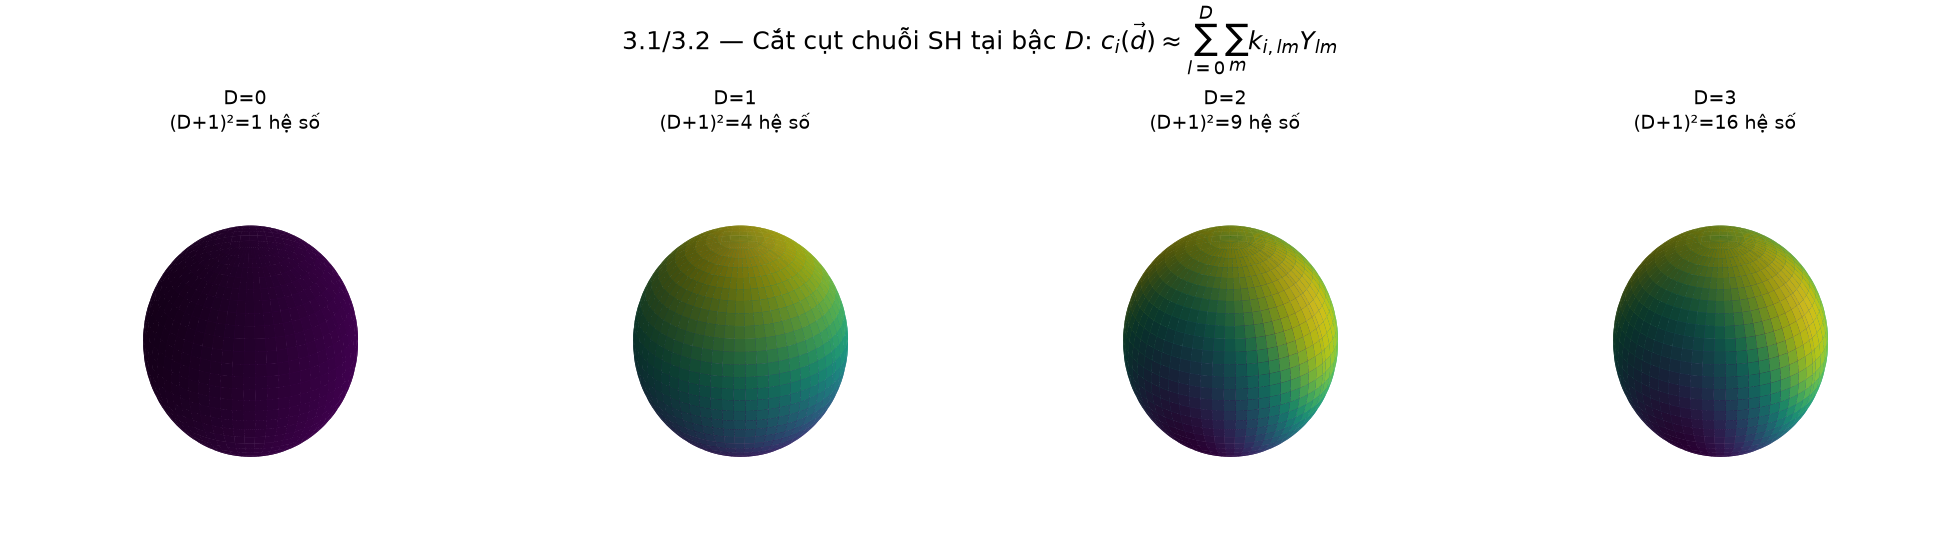
\includegraphics[width=0.9\linewidth]{3_2_truncation_reconstruction.png}
\captionof{figure}{\footnotesize Tái dựng một hàm màu mẫu trên mặt cầu khi tăng dần bậc cắt cụt $D=0,1,2,3$.}
\end{column}
\end{columns}
\end{frame}

% --- 3_2b_coefficient_count.png ---
\begin{frame}{Số hệ số SH: từ $2l+1$ đến $(D+1)^2$}
\begin{columns}[T]
\begin{column}{0.52\linewidth}
\footnotesize
\begin{itemize}
    \item Mỗi bậc $l$ có đúng $2l+1$ hàm cơ sở (ứng với $m=-l,\dots,l$).
    \item Tổng số hệ số cần lưu khi cắt cụt đến bậc $D$:
    $$\sum_{l=0}^{D}(2l+1)=(D+1)^2$$
    \item Bảng cụ thể: $D=0\to1$, $D=1\to4$, $D=2\to9$, $D=3\to16$ hệ số \textbf{mỗi kênh màu}.
    \item Với $D=3$ (dùng trong 3DGS/fastgs-lite): $16$ hệ số $\times\ 3$ kênh RGB $=\mathbf{48}$ số thực mỗi Gaussian cho toàn bộ SH (1 hệ số DC $\times 3$ kênh $=$ \texttt{f\_dc}, còn $45$ hệ số còn lại $=$ \texttt{f\_rest}).
    \item Đây chính là chi phí bộ nhớ/băng thông tối ưu phải trả cho việc biểu diễn màu phụ thuộc góc nhìn.
\end{itemize}
\end{column}
\begin{column}{0.46\linewidth}
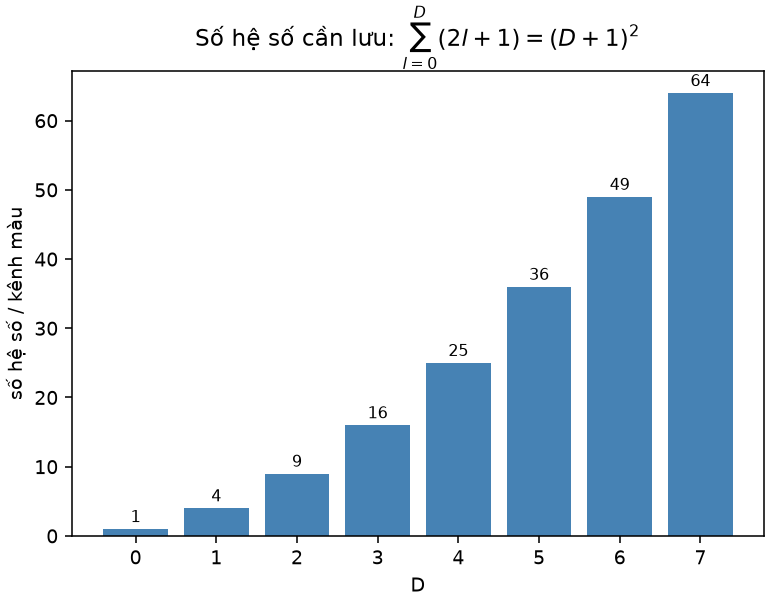
\includegraphics[width=0.9\linewidth]{3_2b_coefficient_count.png}
\captionof{figure}{\footnotesize Số hệ số $(D+1)^2$ theo từng bậc cắt cụt $D$.}
\end{column}
\end{columns}
\end{frame}

% --- 3_3_compute_color_from_sh.png ---
\begin{frame}{Công thức \texttt{computeColorFromSH}: giải mã màu view-dependent}
\footnotesize
Màu quan sát theo hướng nhìn $\vec d$ được tính bằng tổng khai triển SH đến bậc $D=3$:
$$
c_i(\vec d)=\max\!\Bigg(0,\ 0.5+\underbrace{C_0k_{00}}_{l=0}\underbrace{-C_1y\,k_{1,-1}+C_1z\,k_{10}-C_1x\,k_{11}}_{l=1}+\underbrace{\sum_m C_2^{(m)}P_2^{(m)}k_{2m}}_{l=2}+\underbrace{\sum_m C_3^{(m)}P_3^{(m)}k_{3m}}_{l=3}\Bigg)
$$
\begin{itemize}
    \item $C_l^{(m)}=\sqrt{\dfrac{2l+1}{4\pi}\dfrac{(l-|m|)!}{(l+|m|)!}}$: hằng số chuẩn hoá cố định (đã gộp dấu, hoán vị); $P_l^{(m)}(x,y,z)$: đa thức bậc $l$ theo toạ độ hướng nhìn.
    \item $k_{i,lm}$: hệ số khai triển học được của Gaussian $i$ (tham số \texttt{f\_dc}/\texttt{f\_rest}).
    \item $+0.5$: dịch tâm phân bố màu về $[0,1]$ (RGB); $\max(0,\cdot)$: chặn dưới vì tổng SH hữu hạn có thể âm — đạo hàm ngược bị chặn tại nơi bị clamp (lưu trong \texttt{clamped[]}).
    \item Sau bước này, giá trị được clamp/qua sigmoid tuỳ triển khai để ra RGB cuối cùng trong \texttt{gaussian\_renderer/\_\_init\_\_.py} — đây là bước "giải mã" (decode) màu phụ thuộc góc nhìn từ các hệ số SH đã tối ưu.
\end{itemize}
\centering
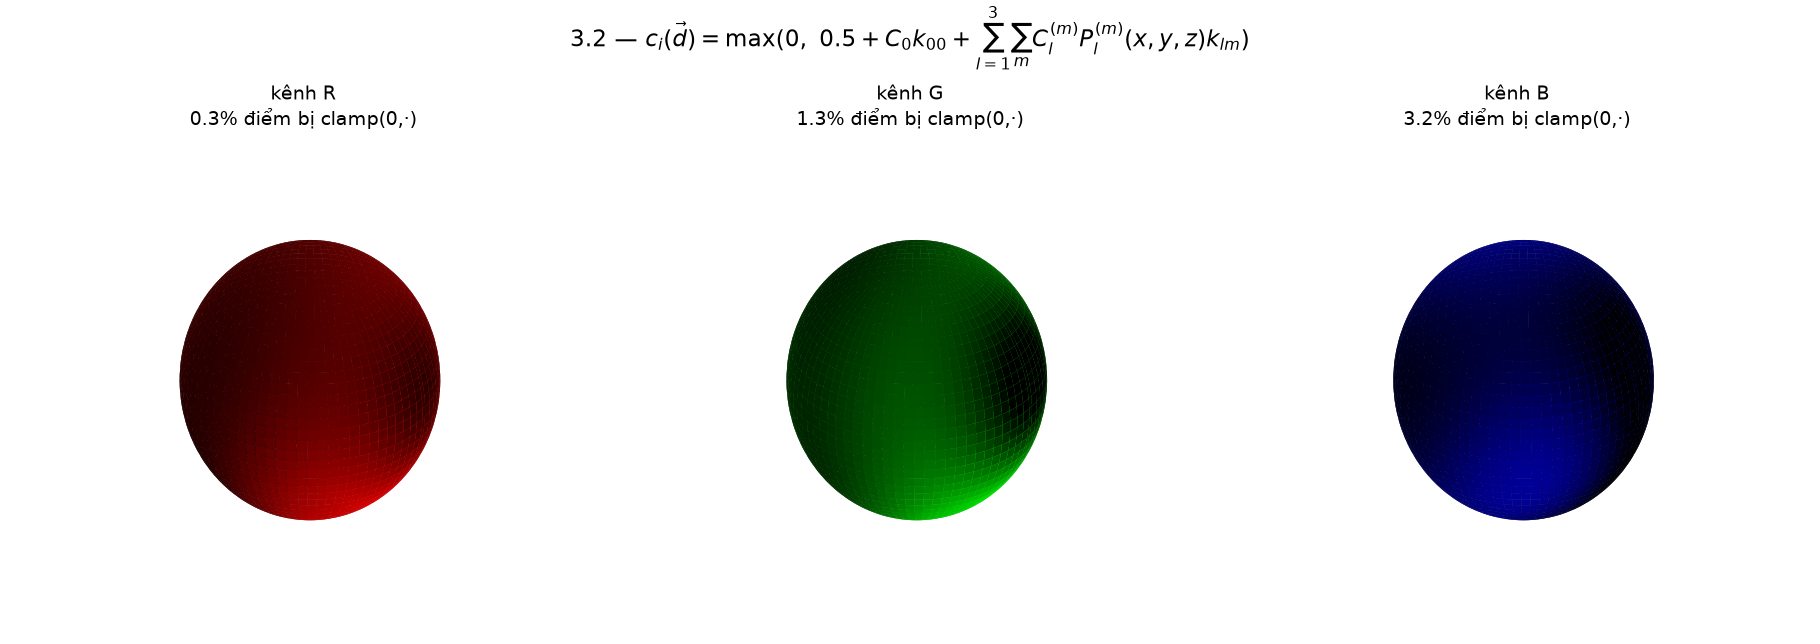
\includegraphics[width=0.55\linewidth]{3_3_compute_color_from_sh.png}
\captionof{figure}{\footnotesize Áp công thức \texttt{computeColorFromSH} đầy đủ ($l=0..3$) cho từng kênh R/G/B với hệ số $k_{lm}$ ngẫu nhiên, vẽ trên mặt cầu; đo tỉ lệ điểm bị $\max(0,\cdot)$ chặn.}
\end{frame}

% --- 3_4_degree_schedule.png ---
\begin{frame}{Lịch tăng bậc SH khi huấn luyện: $D(t)$}
\begin{columns}[T]
\begin{column}{0.52\linewidth}
\footnotesize
\begin{itemize}
    \item Bậc SH đang dùng $D$ không cố định ngay từ đầu mà tăng dần theo bước huấn luyện $t$, dưới dạng hàm bậc thang (không phải PDE hay tối ưu liên tục):
    $$D(t)=\min\!\left(3,\ \left\lfloor\frac{t}{1000}\right\rfloor\right)$$
    \item Bắt đầu $D=0$: chỉ dùng $Y_{00}$ $\Rightarrow$ màu đẳng hướng, không phụ thuộc hướng nhìn (chỉ có \texttt{f\_dc}).
    \item Mỗi $1000$ iteration, $D$ tăng thêm $1$ cho đến khi đạt $D_{\max}=3$, lần lượt "mở khoá" thêm $2l+1$ hệ số bậc cao.
    \item Lý do: khi hình học (vị trí, hiệp phương sai) của Gaussian còn thô/chưa hội tụ, để tối ưu ngay các hệ số bậc cao (specular) dễ gây overfit nhiễu quan sát $\Rightarrow$ tăng dần bậc giúp huấn luyện ổn định hơn, tách biệt học hình học trước, học phản xạ góc nhìn sau.
\end{itemize}
\end{column}
\begin{column}{0.46\linewidth}
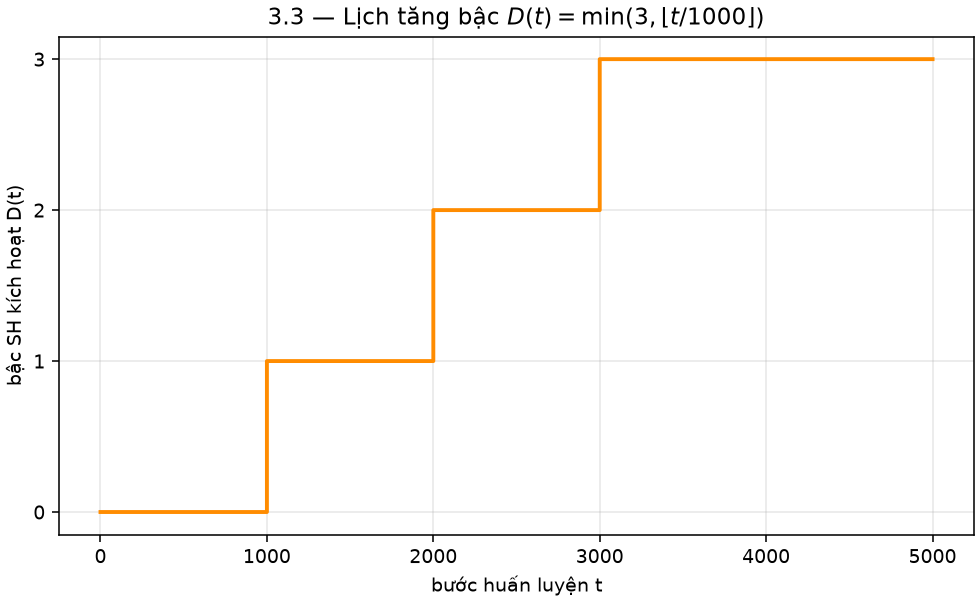
\includegraphics[width=0.9\linewidth]{3_4_degree_schedule.png}
\captionof{figure}{\footnotesize Đồ thị hàm bậc thang $D(t)$ theo bước huấn luyện $t$.}
\end{column}
\end{columns}
\end{frame}

% --- 4_1_parseval_energy.png ---
\begin{frame}{Định lý Parseval trên mặt cầu: năng lượng và hệ số}
\begin{columns}[T]
\begin{column}{0.52\linewidth}
\footnotesize
\begin{itemize}
    \item Do tính trực chuẩn của $\{Y_{lm}\}$, năng lượng ($L^2$-norm bình phương) của hàm màu bằng tổng bình phương các hệ số khai triển:
    $$\int_{S^2}|c_i(\vec d)|^2\,d\Omega=\sum_{l,m}k_{i,lm}^2$$
    \item Cho phép kiểm chứng số học: tích phân số (cầu phương trên lưới $(\theta,\phi)$) vế trái phải khớp tổng bình phương hệ số vế phải.
    \item Phân tách năng lượng theo từng bậc $l$: $\sum_m k_{lm}^2$ cho biết bậc nào "mang" nhiều năng lượng tín hiệu nhất — thực nghiệm cho thấy $l=0$ (DC) chiếm ưu thế áp đảo.
    \item Ứng dụng: đánh giá được \emph{bao nhiêu năng lượng bị mất} khi cắt chuỗi ở bậc $D$ hữu hạn — phần dư $\sum_{l>D}\sum_m k_{lm}^2$ chính là sai số bị bỏ qua.
\end{itemize}
\end{column}
\begin{column}{0.46\linewidth}
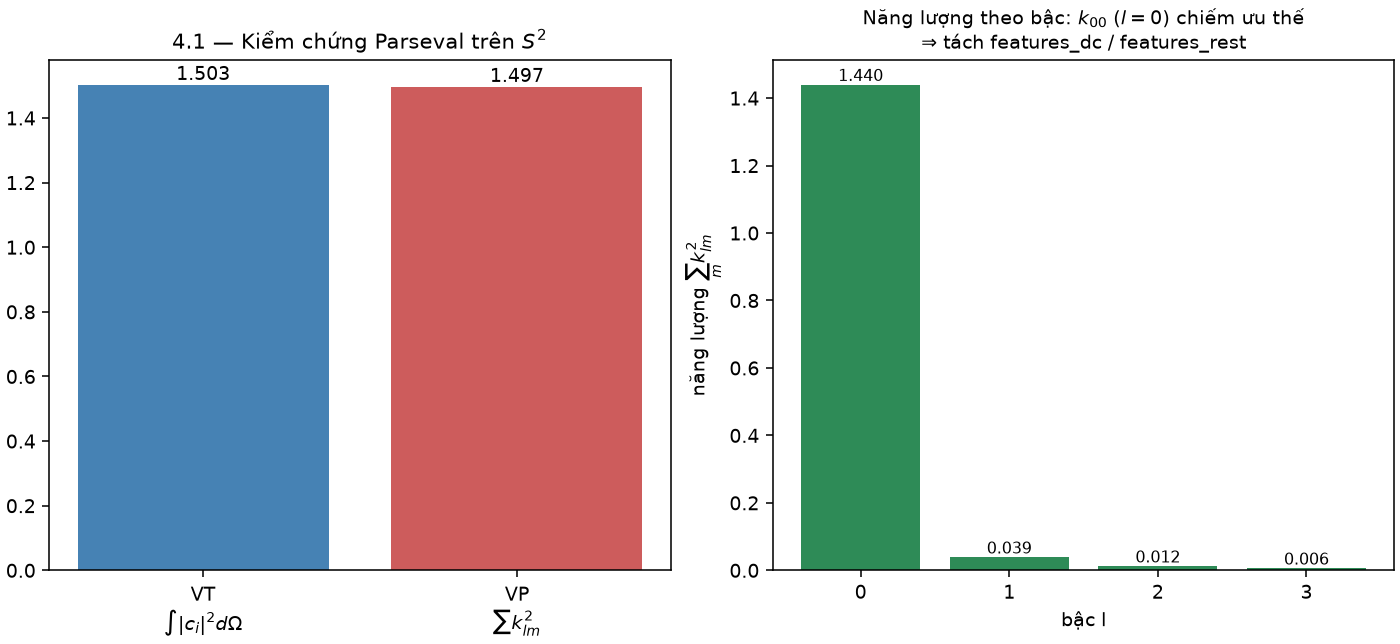
\includegraphics[width=0.9\linewidth]{4_1_parseval_energy.png}
\captionof{figure}{\footnotesize Kiểm chứng số học hai vế Parseval và phân bố năng lượng $\sum_m k_{lm}^2$ theo từng bậc $l$ (cho thấy $l=0$ chiếm ưu thế).}
\end{column}
\end{columns}
\end{frame}

% --- 4_2_mean_color_dc.png ---
\begin{frame}{Hệ số DC $k_{00}$: chính là màu trung bình}
\begin{columns}[T]
\begin{column}{0.52\linewidth}
\footnotesize
\begin{itemize}
    \item Vì $Y_{00}=C_0=\frac12\sqrt{1/\pi}$ là hằng số, còn mọi $Y_{lm}$ với $l\ge1$ có trung bình bằng $0$ trên mặt cầu (trực giao với hàm hằng $Y_{00}$), nên lấy trung bình đều hướng nhìn của $c_i$:
    $$\bar c_i=\frac{1}{4\pi}\int_{S^2}c_i(\vec d)\,d\Omega = C_0\,k_{i,00}$$
    \item Đây là lý do khởi tạo \texttt{f\_dc = RGB2SH(color)} dùng đúng quan hệ nghịch đảo $k_{00}=\bar c_i / C_0$ để hệ số bậc $0$ khớp chính xác màu quan sát trung bình ban đầu (trước khi có thông tin về phụ thuộc góc nhìn).
    \item Vì $k_{00}$ chiếm phần lớn năng lượng tín hiệu màu (theo Parseval ở slide trước), nó cần learning rate \emph{thấp} để tránh dao động màu toàn ảnh.
    \item Ngược lại, $45$ hệ số bậc $l=1..3$ (\texttt{f\_rest}) chỉ là nhiễu loạn nhỏ bậc cao mã hoá hiệu ứng phản xạ/specular $\Rightarrow$ tách optimizer riêng, cập nhật thưa hơn.
\end{itemize}
\end{column}
\begin{column}{0.46\linewidth}
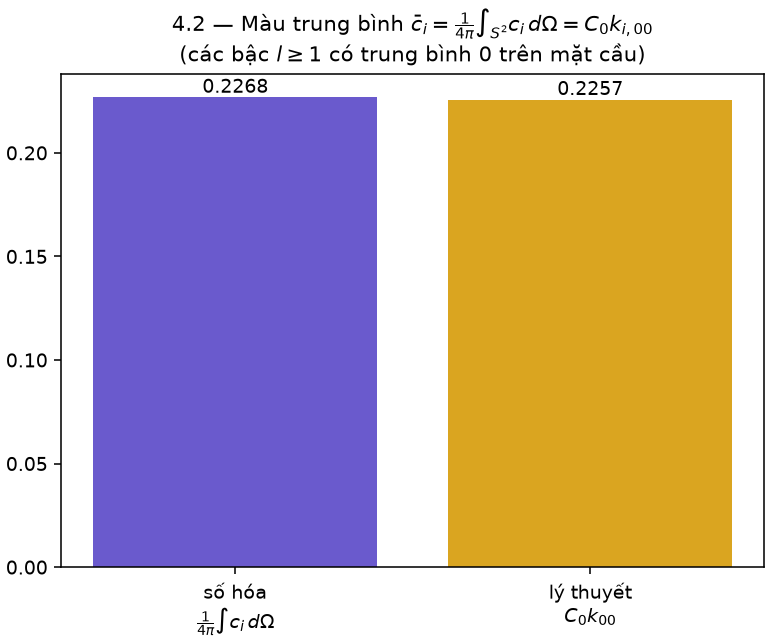
\includegraphics[width=0.9\linewidth]{4_2_mean_color_dc.png}
\captionof{figure}{\footnotesize So sánh trung bình số học $\frac{1}{4\pi}\int c_i\,d\Omega$ (tích phân số trên lưới cầu) với công thức lý thuyết $C_0 k_{00}$.}
\end{column}
\end{columns}
\end{frame}


% ===================== PHẦN 2 =====================
\section{Chiếu phối cảnh \& Rasterizer khả vi}
% --- Slide 11 ---
\begin{frame}{Tổng quan pipeline render}
    \begin{itemize}
        \item World $\to$ Camera: biến đổi hệ toạ độ bằng view transform $(R, t)$
        \item Projection: chiếu các Gaussian 3D xuống mặt phẳng ảnh 2D
        \item Tiling: xác định tile ảnh nào chịu ảnh hưởng bởi mỗi Gaussian
        \item Sorting: sắp xếp Gaussian theo độ sâu (depth) trong từng tile
        \item Alpha blending tuần tự $\to$ màu pixel cuối cùng
    \end{itemize}
    \vspace{0.3cm}
    \centering
    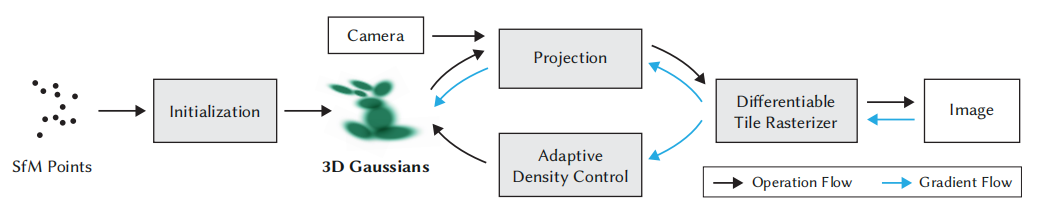
\includegraphics[width=0.95\linewidth]{pipe.png}
    \captionof{figure}{Pipeline render 3D Gaussian Splatting}
\end{frame}

% --- Slide 12 ---
\begin{frame}{Chiếu camera pinhole}
    \begin{columns}
        \begin{column}{0.48\textwidth}
            \begin{itemize}
                \item World $\to$ Camera: nhân với ma trận quay $R$ và tịnh tiến $t$
                \item Chiếu phối cảnh theo mô hình pinhole với tiêu cự $f$ và điểm chính (principal point)
                \item Công thức chiếu cơ bản:
                \[
                    x' = f\frac{x}{z}, \qquad y' = f\frac{y}{z}
                \]
                \item Kết quả: toạ độ tâm Gaussian trên ảnh 2D
            \end{itemize}
        \end{column}
        \begin{column}{0.48\textwidth}
            \centering
            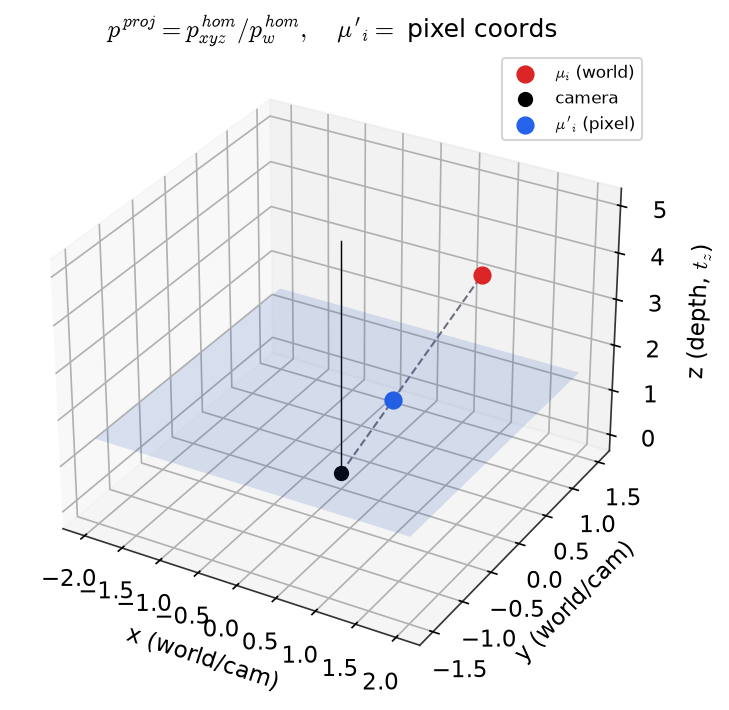
\includegraphics[width=0.95\linewidth]{ch3_pinhole_projection.png}
            \captionof{figure}{Mô hình chiếu pinhole}
        \end{column}
    \end{columns}
\end{frame}

% --- Slide 13 ---
\begin{frame}{Chiếu hiệp phương sai (EWA splatting)}
    \begin{itemize}
        \item Phép chiếu phối cảnh phi tuyến $\to$ xấp xỉ tuyến tính cục bộ bằng Jacobian $J$ tại tâm Gaussian
        \item Hiệp phương sai 2D sau chiếu:
        \[
            \Sigma' = J\,W\,\Sigma\,W^{T}J^{T}
        \]
        trong đó $W$ là phần quay của view matrix
        \item Kết quả: một ellipse 2D trên ảnh cho mỗi Gaussian 3D
        \item Kỹ thuật này gọi là \textbf{Elliptical Weighted Average (EWA) splatting}
    \end{itemize}
    \vspace{0.2cm}
    \centering
    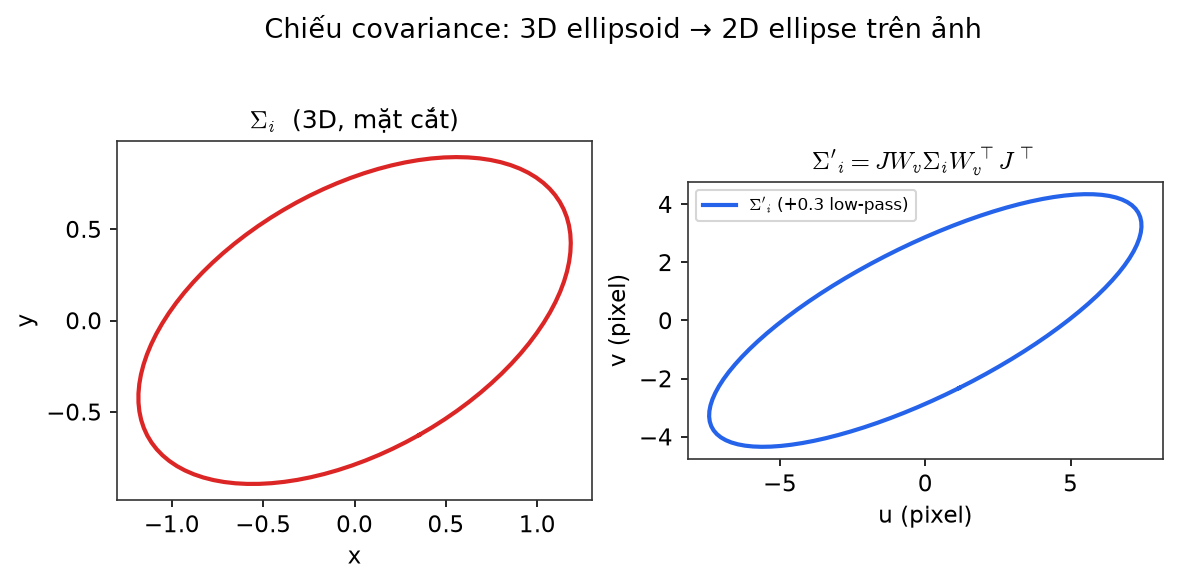
\includegraphics[width=0.6\linewidth]{ch3_ewa_projection.png}
    \captionof{figure}{Chiếu hiệp phương sai theo EWA splatting}
\end{frame}

% --- Slide 14 ---
\begin{frame}{Compact Box -- đòn bẩy tăng tốc \#1 của FastGS}
\begin{columns}[T]
\begin{column}{0.52\textwidth}
\footnotesize
    \begin{itemize}
        \item Mặc định: bounding-box $3\sigma$ -- khá rộng, chạm nhiều tile không cần thiết
        \item FastGS thay bằng \textbf{compact box}: vùng ảnh hưởng 2D nhỏ hơn, điều chỉnh bằng hệ số \texttt{-{}-mult}
        \item Mặc định \texttt{mult = 0.5}; tăng lên \texttt{0.7} cho cảnh lớn/phức tạp
        \item Kết quả: giảm đáng kể số tile mỗi Gaussian phải rasterize
    \end{itemize}
\end{column}
\begin{column}{0.48\textwidth}
    \centering
    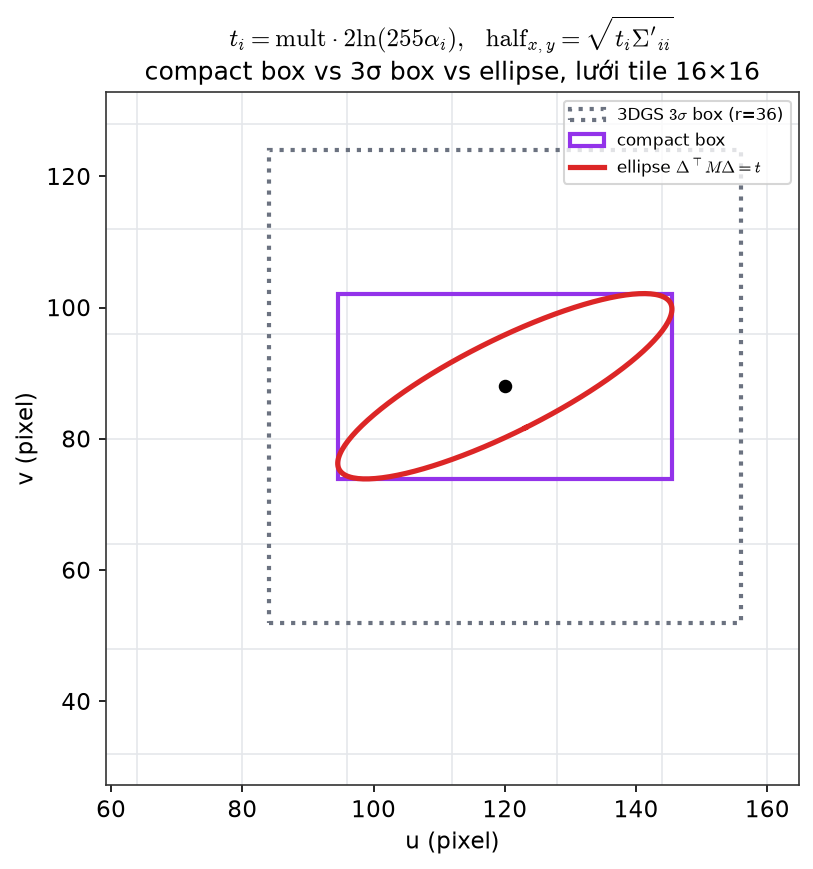
\includegraphics[width=0.95\linewidth]{ch3_compact_box.png}
    \captionof{figure}{\footnotesize So sánh bounding-box mặc định và compact box}
\end{column}
\end{columns}
\end{frame}

% --- Slide 15 ---
\begin{frame}{Tỉ lệ diện tích ảnh hưởng tile}
\begin{columns}[T]
\begin{column}{0.5\textwidth}
\footnotesize
    \begin{itemize}
        \item Số tile bị một Gaussian "chạm" tỉ lệ thuận với diện tích ellipse chiếu của nó trên ảnh
        \item Compact box giúp giảm tỉ lệ diện tích này mà không làm giảm chất lượng render đáng kể
        \item Đây là cơ sở lý thuyết cho việc tăng tốc rasterization của FastGS
    \end{itemize}
\end{column}
\begin{column}{0.5\textwidth}
    \centering
    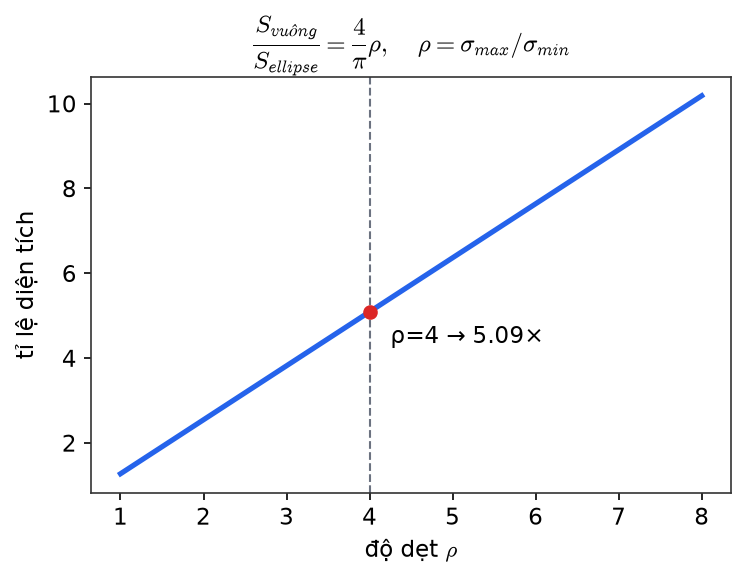
\includegraphics[width=0.95\linewidth]{ch3_area_ratio.png}
    \captionof{figure}{\footnotesize Tỉ lệ diện tích ảnh hưởng khi thay đổi compact box}
\end{column}
\end{columns}
\end{frame}

% --- Slide 16 ---
\begin{frame}{Rasterizer khả vi theo tile (CUDA)}
    \begin{itemize}
        \item Ảnh được chia thành lưới tile (ví dụ $16 \times 16$ pixel)
        \item Mỗi tile lưu danh sách các Gaussian chạm tới nó
        \item Danh sách này được sort theo độ sâu (depth) trước khi blend
        \item Xử lý song song trên GPU: mỗi thread-block CUDA đảm nhận một tile
        \item Cài đặt trong module \texttt{submodules/diff-gaussian-rasterization\_fastgs/}
        \item Toàn bộ quá trình khả vi $\to$ hỗ trợ lan truyền ngược gradient
    \end{itemize}
\end{frame}

% --- Slide 17 ---
\begin{frame}{Trường alpha (opacity field)}
\begin{columns}[T]
\begin{column}{0.52\textwidth}
\footnotesize
    \begin{itemize}
        \item Mỗi Gaussian 2D đã chiếu tạo ra một trường độ mờ liên tục trên ảnh
        \item Công thức trường alpha:
        \[
            \alpha(p) = \alpha_i \cdot G'_i(p)
        \]
        \item $G'_i$ là hàm Gaussian 2D chuẩn hoá theo hiệp phương sai $\Sigma'$
        \item Giá trị $\alpha(p)$ càng lớn khi $p$ càng gần tâm ellipse
    \end{itemize}
\end{column}
\begin{column}{0.48\textwidth}
    \centering
    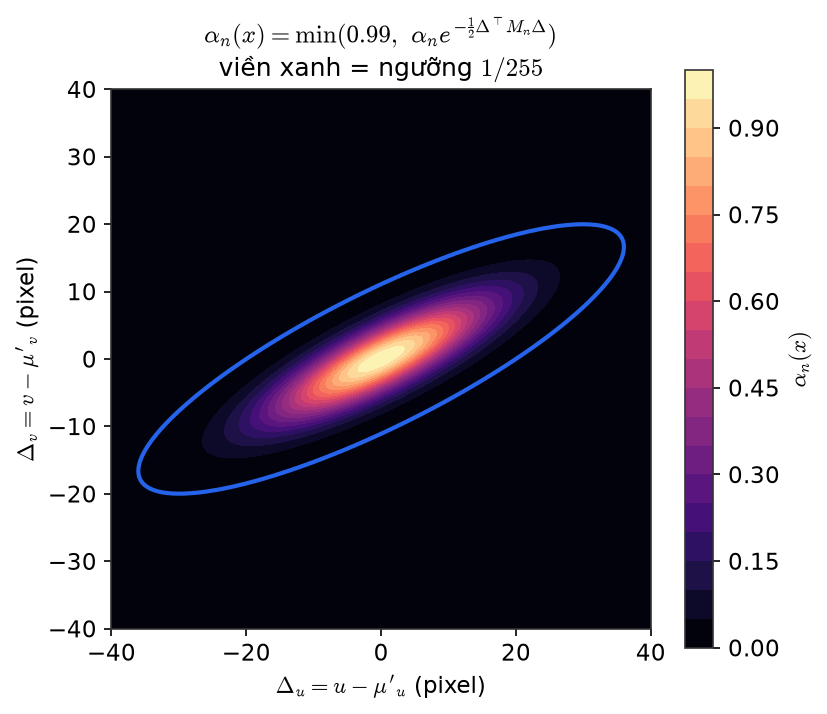
\includegraphics[width=0.85\linewidth]{ch4_alpha_field.png}
    \captionof{figure}{\footnotesize Trường alpha của một Gaussian 2D}
\end{column}
\end{columns}
\end{frame}

% --- Slide 18 ---
\begin{frame}{Alpha blending (front-to-back)}
    \begin{itemize}
        \item Màu pixel là tổng có trọng số của các Gaussian chồng nhau theo thứ tự độ sâu
        \item Công thức blend:
        \[
            C = \sum_i c_i\,\alpha_i\,T_i, \qquad T_i = \prod_{j<i}(1-\alpha_j)
        \]
        \item $T_i$: độ truyền sáng còn lại (transmittance) trước Gaussian thứ $i$
        \item Gaussian gần camera hơn đóng góp trọng số lớn hơn
    \end{itemize}
    \vspace{0.2cm}
    \centering
    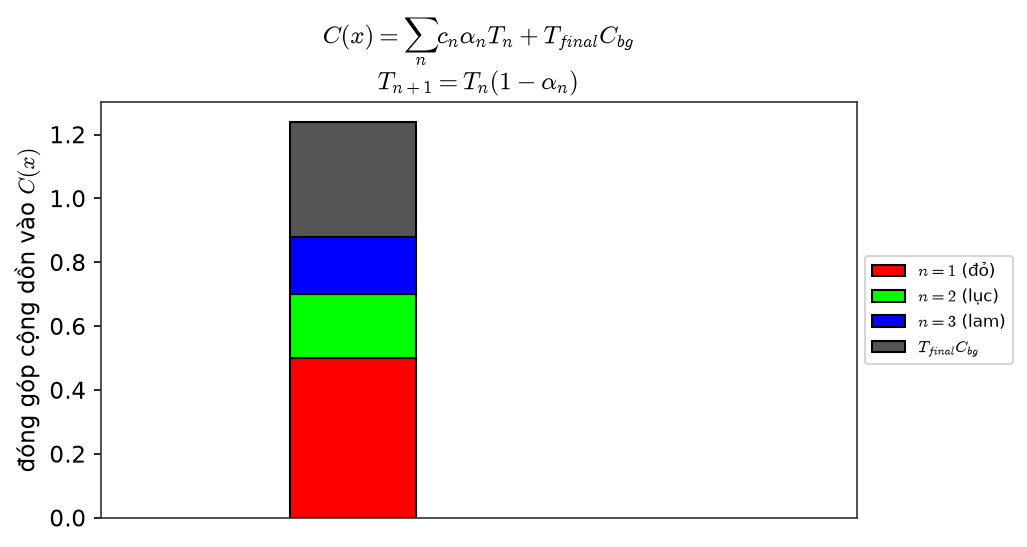
\includegraphics[width=0.55\linewidth]{ch4_alpha_blend_stack.png}
    \captionof{figure}{Chồng lớp alpha blending theo độ sâu}
\end{frame}

% --- Slide 19 ---
\begin{frame}{Suy giảm độ truyền sáng (transmittance decay)}
\begin{columns}[T]
\begin{column}{0.52\textwidth}
\footnotesize
    \begin{itemize}
        \item $T_i$ giảm dần theo cấp số nhân khi càng nhiều Gaussian che phía trước
        \item Khi $T_i \approx 0$: các Gaussian phía sau gần như không đóng góp vào màu pixel
        \item Cho phép \textbf{early stopping}: dừng xử lý sớm để tối ưu tốc độ render
        \item Đây là một trong các kỹ thuật tăng tốc quan trọng của rasterizer
    \end{itemize}
\end{column}
\begin{column}{0.48\textwidth}
    \centering
    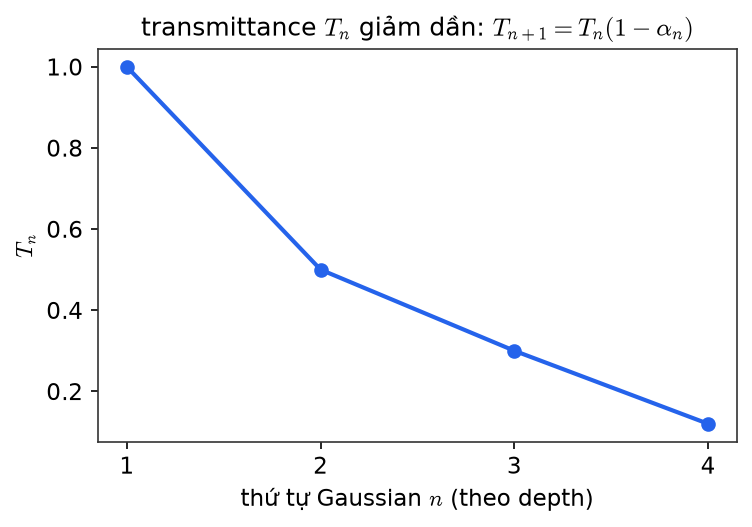
\includegraphics[width=0.9\linewidth]{ch4_transmittance_decay.png}
    \captionof{figure}{\footnotesize Suy giảm transmittance theo số lớp Gaussian}
\end{column}
\end{columns}
\end{frame}

% --- Slide 20 ---
\begin{frame}{Tổng kết phương trình render}
    \begin{itemize}
        \item Phương trình render đầy đủ:
        \[
            C(p) = \sum_i c_i\,\alpha_i \prod_{j<i}(1-\alpha_j)
        \]
        \item Khả vi theo mọi tham số: vị trí $\mu$, hiệp phương sai $\Sigma$, độ mờ $\alpha$, hệ số SH
        \item Cho phép huấn luyện trực tiếp bằng gradient descent từ ảnh RGB quan sát được
    \end{itemize}
    \vspace{0.4cm}
    \centering
    \begin{tikzpicture}[node distance=1.1cm, every node/.style={font=\footnotesize}]
        \node (g3d) {Gaussian 3D};
        \node (proj) [right=of g3d] {Chiếu 2D};
        \node (alpha) [right=of proj] {Trường alpha};
        \node (blend) [right=of alpha] {Blend};
        \node (pixel) [right=of blend] {Pixel};
        \draw[-Latex] (g3d) -- (proj);
        \draw[-Latex] (proj) -- (alpha);
        \draw[-Latex] (alpha) -- (blend);
        \draw[-Latex] (blend) -- (pixel);
    \end{tikzpicture}
\end{frame}


% ===================== PHẦN 3 =====================
\section{Loss, Gradient \& Optimizer}
% ==============================================
% PHẦN 3 (Slide 21--30): Hàm mất mát, Metric đánh giá,
% Gradient và Optimizer trong huấn luyện 3DGS
% ==============================================

% --- Slide 21 ---
\begin{frame}{Hàm mất mát: kết hợp L1 và D-SSIM}
    \begin{columns}[T]
        \begin{column}{0.5\textwidth}
            \begin{itemize}
                \item Loss huấn luyện kết hợp hai thành phần bổ trợ nhau:
                \begin{itemize}
                    \item \textbf{L1}: sai khác trung bình theo từng pixel.
                    \item \textbf{D-SSIM}: $1-\text{SSIM}$, phản ánh sai lệch \textbf{cấu trúc}.
                \end{itemize}
                \item Công thức tổng:
                \[
                    \mathcal{L} = (1-\lambda)\,\mathcal{L}_1 + \lambda\,(1-\text{SSIM})
                \]
                \item Hệ số $\lambda = $ \texttt{lambda\_dssim}:
                \begin{itemize}
                    \item Mặc định: $0.2$
                    \item \texttt{fastgs-lite}: $0.25$ (nhấn mạnh cấu trúc hơn)
                \end{itemize}
            \end{itemize}
        \end{column}
        \begin{column}{0.5\textwidth}
            \centering
            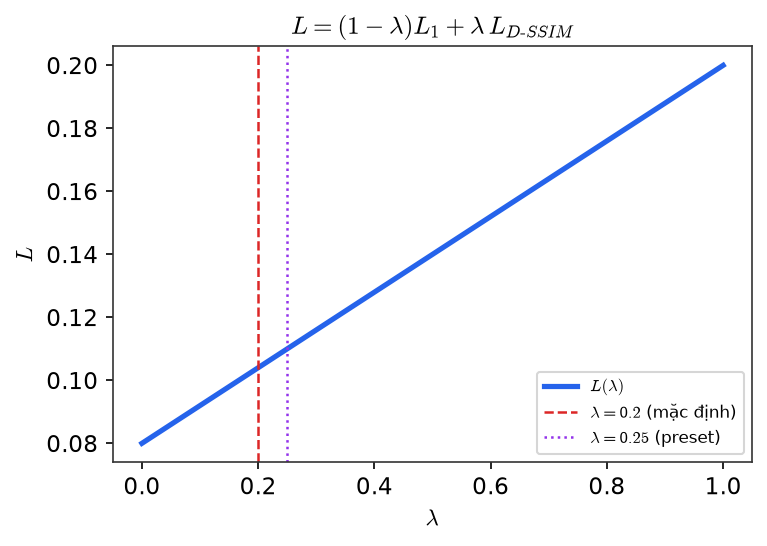
\includegraphics[width=0.95\linewidth]{ch5_loss_mix.png}
            \captionof{figure}{Tỉ trọng L1 và D-SSIM trong loss}
        \end{column}
    \end{columns}
\end{frame}

% --- Slide 22 ---
\begin{frame}{SSIM: so sánh theo cửa sổ trượt}
    \begin{columns}[T]
        \begin{column}{0.5\textwidth}
            \begin{itemize}
                \item SSIM không so sánh pixel đơn lẻ mà trượt một \textbf{cửa sổ nhỏ} (thường $11\times 11$) trên ảnh render và ảnh gốc.
                \item Trong mỗi cửa sổ, kết hợp 3 yếu tố:
                \begin{itemize}
                    \item Độ sáng (luminance)
                    \item Độ tương phản (contrast)
                    \item Cấu trúc (structure)
                \end{itemize}
                \item Nhạy với sai lệch \textbf{cấu trúc cục bộ} hơn hẳn L1/L2 thuần pixel.
                \item Do đó bổ sung tốt cho L1 trong hàm loss.
            \end{itemize}
        \end{column}
        \begin{column}{0.5\textwidth}
            \centering
            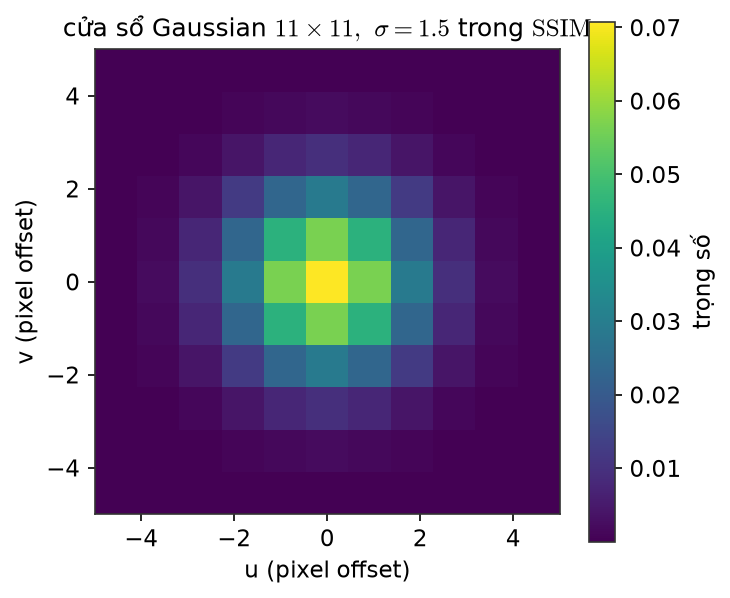
\includegraphics[width=0.95\linewidth]{ch5_ssim_window.png}
            \captionof{figure}{Cửa sổ trượt khi tính SSIM}
        \end{column}
    \end{columns}
\end{frame}

% --- Slide 23 ---
\begin{frame}{PSNR: metric per-pixel}
    \begin{columns}[T]
        \begin{column}{0.5\textwidth}
            \begin{itemize}
                \item PSNR (Peak Signal-to-Noise Ratio) đo theo dB, dựa trên MSE giữa ảnh render và ảnh gốc:
                \[
                    \text{PSNR} = 10 \cdot \log_{10}\!\left(\frac{\text{MAX}^2}{\text{MSE}}\right)
                \]
                \item PSNR càng cao $\Rightarrow$ sai số pixel càng nhỏ.
                \item Nhược điểm: là metric \textbf{per-pixel thuần}, không phản ánh tốt chất lượng \textbf{cảm nhận thị giác} như SSIM hay LPIPS.
            \end{itemize}
        \end{column}
        \begin{column}{0.5\textwidth}
            \centering
            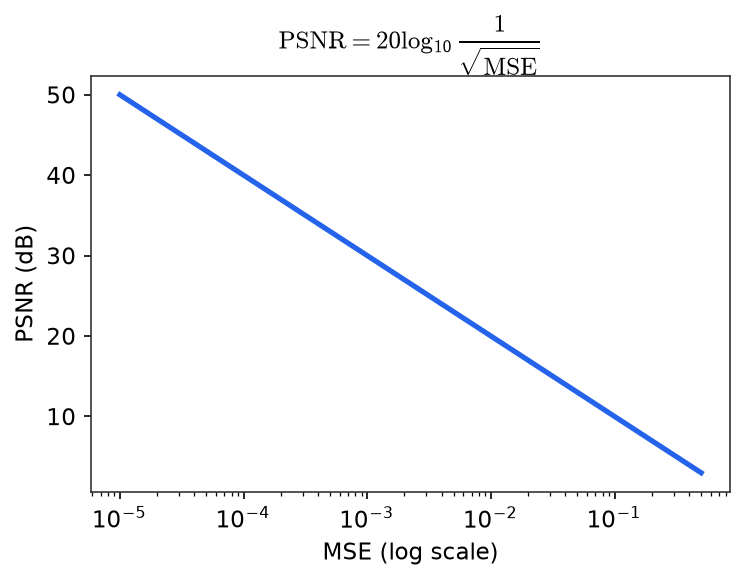
\includegraphics[width=0.95\linewidth]{ch5_psnr.png}
            \captionof{figure}{Quan hệ MSE và PSNR (dB)}
        \end{column}
    \end{columns}
\end{frame}

% --- Slide 24 ---
\begin{frame}{Điểm số tổng hợp (Score) đánh giá benchmark}
    \begin{columns}[T]
        \begin{column}{0.5\textwidth}
            \footnotesize
            \begin{itemize}
                \item Công thức điểm dùng trong benchmark/cuộc thi, kết hợp cả 3 metric:
                \[
                    \text{Score} = 0.4(1-\text{LPIPS}) + 0.3\,\text{SSIM} + 0.3\,\text{clamp}\!\left(\frac{\text{PSNR}}{\text{PSNR}_{\max}}, 0, 1\right)
                \]
                với $\text{PSNR}_{\max} = 30$dB.
                \item Mục tiêu: cân bằng giữa
                \begin{itemize}
                    \item độ chính xác pixel (PSNR),
                    \item cấu trúc (SSIM),
                    \item cảm nhận thị giác (LPIPS).
                \end{itemize}
            \end{itemize}
        \end{column}
        \begin{column}{0.5\textwidth}
            \centering
            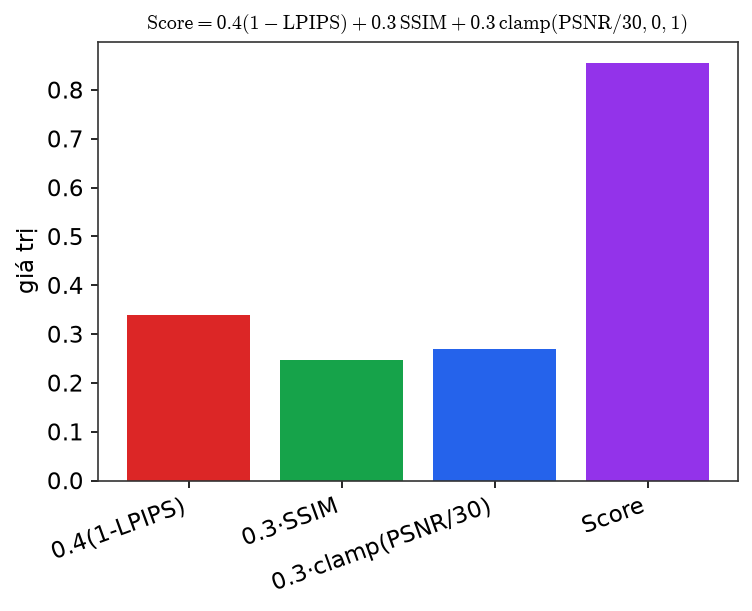
\includegraphics[width=0.95\linewidth]{ch5_score_decomp.png}
            \captionof{figure}{Phân rã đóng góp của Score}
        \end{column}
    \end{columns}
\end{frame}

% --- Slide 25 ---
\begin{frame}{Lan truyền gradient qua rasterizer khả vi}
    \begin{itemize}
        \item Phép render 3DGS (chiếu Gaussian + alpha blending) hoàn toàn \textbf{khả vi}, nên có thể lan truyền ngược (backprop) từ loss về từng tham số Gaussian.
        \item Chuỗi lan truyền ngược:
    \end{itemize}
    \begin{center}
        \footnotesize
        pixel $\xrightarrow{\ \partial\ }$ alpha blend $\xrightarrow{\ \partial\ }$ alpha field $\xrightarrow{\ \partial\ }$ covariance chiếu $\xrightarrow{\ \partial\ }$ $(\mu, \Sigma)$ gốc
    \end{center}
    \begin{itemize}
        \item Quy tắc chuỗi (chain rule) tổng quát cho mỗi tham số $\theta \in \{\mu, \Sigma, \alpha, \text{SH}\}$:
        \[
            \frac{\partial \mathcal{L}}{\partial \theta} = \frac{\partial \mathcal{L}}{\partial C} \cdot \frac{\partial C}{\partial \theta}
        \]
        \item Nhờ đó mọi tham số Gaussian đều được cập nhật trực tiếp từ tín hiệu loss ở không gian ảnh.
    \end{itemize}
\end{frame}

% --- Slide 26 ---
\begin{frame}{Gradient tập trung tại biên Gaussian}
    \begin{columns}[T]
        \begin{column}{0.5\textwidth}
            \begin{itemize}
                \item Gradient view-space lớn nhất xuất hiện ở vùng \textbf{biên/rìa} của Gaussian.
                \item Đây là nơi ảnh render lệch nhiều nhất so với ảnh thật (sai số cao).
                \item Ý nghĩa quan trọng: gradient tại biên chính là \textbf{tín hiệu} dùng để quyết định \textbf{densify} (thêm Gaussian mới) ở giai đoạn sau.
                \item Vùng gradient thấp $\Rightarrow$ Gaussian đã khớp tốt, không cần chia tách thêm.
            \end{itemize}
        \end{column}
        \begin{column}{0.5\textwidth}
            \centering
            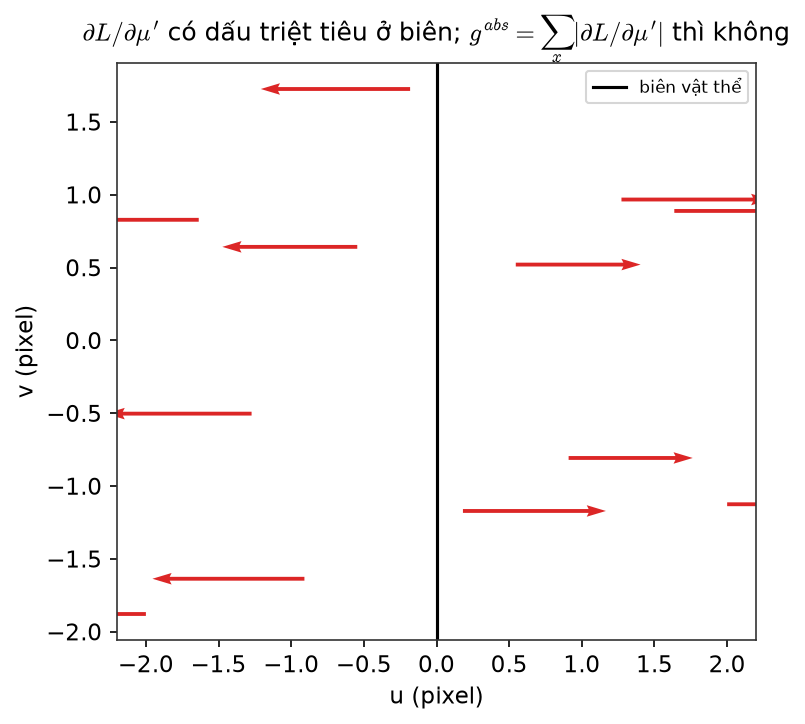
\includegraphics[width=0.95\linewidth]{ch6_edge_gradient.png}
            \captionof{figure}{Gradient tập trung ở biên Gaussian}
        \end{column}
    \end{columns}
\end{frame}

% --- Slide 27 ---
\begin{frame}{Adam optimizer cho từng tham số Gaussian}
    \begin{columns}[T]
        \begin{column}{0.5\textwidth}
            \begin{itemize}
                \item Mỗi tham số Gaussian ($\mu, \Sigma, \alpha, \text{SH}$) có trạng thái Adam riêng:
                \begin{itemize}
                    \item Moment bậc 1 (trung bình gradient)
                    \item Moment bậc 2 (trung bình bình phương gradient)
                \end{itemize}
                \item Learning rate thích ứng (adaptive) theo từng chiều tham số.
                \item Quỹ đạo hội tụ \textbf{mượt hơn} so với SGD thuần, tránh dao động mạnh khi gradient nhiễu.
            \end{itemize}
        \end{column}
        \begin{column}{0.5\textwidth}
            \centering
            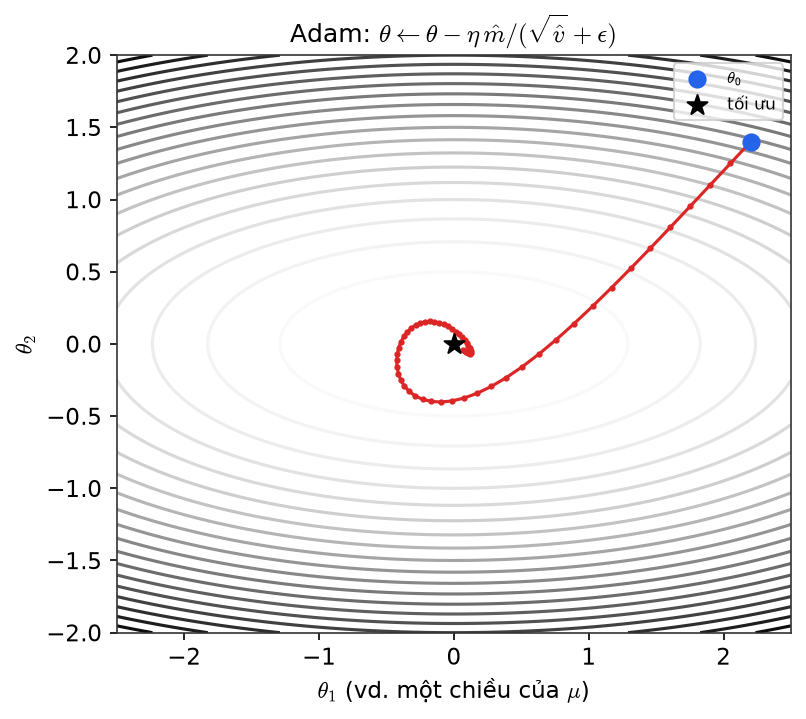
\includegraphics[width=0.95\linewidth]{ch6_adam_trajectory.png}
            \captionof{figure}{Quỹ đạo cập nhật của Adam}
        \end{column}
    \end{columns}
\end{frame}

% --- Slide 28 ---
\begin{frame}{Lịch suy giảm learning rate}
    \begin{columns}[T]
        \begin{column}{0.5\textwidth}
            \begin{itemize}
                \item Learning rate của từng nhóm tham số (đặc biệt là vị trí $\mu$) giảm dần theo \textbf{hàm mũ} (exponential decay).
                \item Suy giảm diễn ra qua số bước \texttt{position\_lr\_max\_steps}.
                \item Mục đích:
                \begin{itemize}
                    \item Học nhanh, bước lớn ở giai đoạn đầu.
                    \item Ổn định, tinh chỉnh nhỏ dần về cuối huấn luyện.
                \end{itemize}
            \end{itemize}
        \end{column}
        \begin{column}{0.5\textwidth}
            \centering
            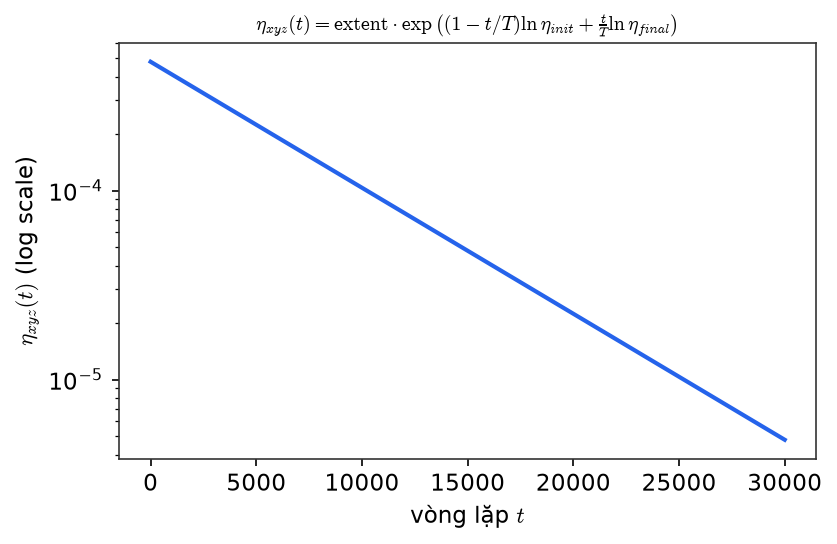
\includegraphics[width=0.95\linewidth]{ch6_lr_decay.png}
            \captionof{figure}{Suy giảm learning rate theo hàm mũ}
        \end{column}
    \end{columns}
\end{frame}

% --- Slide 29 ---
\begin{frame}{Sparse Adam schedule (đòn bẩy tăng tốc \#3)}
    \begin{columns}[T]
        \begin{column}{0.5\textwidth}
            \footnotesize
            \begin{itemize}
                \item Không phải mọi tham số được cập nhật ở mọi iteration.
                \item \texttt{features\_rest} (SH bậc cao, chi phối màu view-dependent):
                \begin{itemize}
                    \item Chỉ \texttt{step} mỗi \textbf{16} iteration đến 15k.
                \end{itemize}
                \item Sau đó, mọi tham số:
                \begin{itemize}
                    \item \texttt{step} mỗi \textbf{32} iteration (15k--20k)
                    \item \texttt{step} mỗi \textbf{64} iteration (sau 20k)
                \end{itemize}
                \item Giảm mạnh chi phí \texttt{optimizer.step()}, gần như không ảnh hưởng chất lượng vì thành phần SH bậc cao thay đổi chậm.
            \end{itemize}
        \end{column}
        \begin{column}{0.5\textwidth}
            \centering
            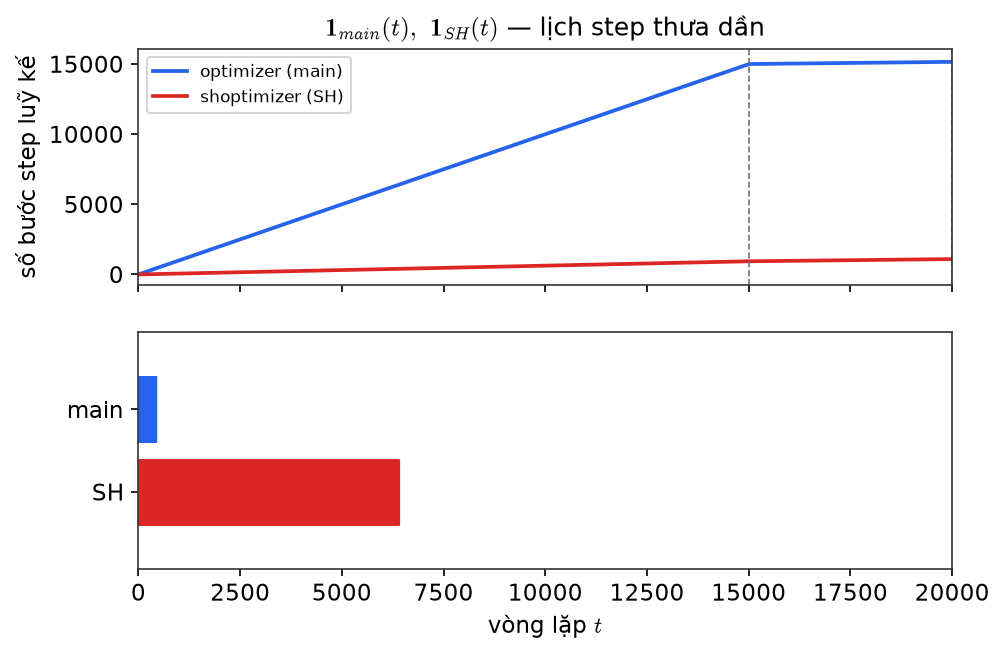
\includegraphics[width=0.95\linewidth]{ch6_step_schedule.png}
            \captionof{figure}{Lịch step thưa của Sparse Adam}
        \end{column}
    \end{columns}
\end{frame}

% --- Slide 30 ---
\begin{frame}{Tổng kết vòng lặp huấn luyện}
    \begin{center}
        \footnotesize
        \begin{tikzpicture}[
            node distance=1.1cm and 1.6cm,
            box/.style={draw, rounded corners, fill=blue!8, align=center, minimum width=2.6cm, minimum height=1cm},
            ->, thick
        ]
            \node[box] (render) {1. Render};
            \node[box, right=of render] (loss) {2. Tính loss\\ (L1 + D-SSIM)};
            \node[box, right=of loss] (backward) {3. Backward\\ (lan gradient)};
            \node[box, below=of loss] (step) {4. optimizer.step()\\ (sparse Adam)};
            \node[box, left=of step] (dp) {5. Densify /\\ Prune (định kỳ)};

            \draw (render) -- (loss);
            \draw (loss) -- (backward);
            \draw (backward) |- (step);
            \draw (step) -- (dp);
            \draw (dp) |- (render);
        \end{tikzpicture}
    \end{center}
    \begin{itemize}
        \item Một iteration: \textbf{render} $\to$ \textbf{tính loss} $\to$ \textbf{backward} $\to$ \textbf{optimizer.step()} $\to$ (định kỳ) \textbf{densify/prune} $\to$ lặp lại.
        \item Vòng lặp này chạy hàng chục nghìn iteration cho đến khi hội tụ.
    \end{itemize}
\end{frame}


% ===================== PHẦN 4 (ADC tổng quan) =====================
\section{Adaptive Density Control — Tổng quan}
% ============================================================
% PHẦN 4 (Slide 31--40): Adaptive Density Control (ADC)
% ============================================================

% --- Slide 31 ---
\begin{frame}{Tổng quan Adaptive Density Control (ADC)}
    \begin{itemize}
        \item Point cloud khởi tạo từ COLMAP thường \textbf{quá thưa} ở vùng thiếu chi tiết, đồng thời có Gaussian \textbf{quá to} che khuất chi tiết nhỏ.
        \item ADC chạy định kỳ mỗi \texttt{densification\_interval} iteration trong lúc train để điều chỉnh mật độ Gaussian.
        \item Hai nhóm thao tác chính:
        \begin{itemize}
            \item \textbf{Densify}: nhân bản (clone) hoặc tách (split) Gaussian thiếu hình học.
            \item \textbf{Prune}: cắt tỉa Gaussian thừa, mờ, hoặc vô dụng.
        \end{itemize}
        \item Mục tiêu: cân bằng giữa chất lượng tái tạo và số lượng Gaussian (chi phí bộ nhớ, tốc độ render).
    \end{itemize}
    \vspace{0.3cm}
    \centering
    \begin{tikzpicture}[node distance=1.6cm, every node/.style={font=\footnotesize}]
        \node[draw, rounded corners, fill=blue!10] (adc) {ADC};
        \node[draw, rounded corners, fill=green!10, below left=1.0cm and 1.8cm of adc] (clone) {Clone};
        \node[draw, rounded corners, fill=orange!10, below=1.4cm of adc] (split) {Split};
        \node[draw, rounded corners, fill=red!10, below right=1.0cm and 1.8cm of adc] (prune) {Prune};
        \draw[->] (adc) -- (clone);
        \draw[->] (adc) -- (split);
        \draw[->] (adc) -- (prune);
    \end{tikzpicture}
\end{frame}

% --- Slide 32 ---
\begin{frame}{Dòng thời gian densify/prune}
    \footnotesize
    \begin{itemize}
        \item \texttt{densify\_from\_iter}: bắt đầu cho phép densify (thường bỏ qua vài trăm iteration đầu để scene ổn định).
        \item Mỗi \texttt{densification\_interval} iteration: chạy một vòng \textbf{clone/split} dựa trên gradient tích luỹ.
        \item Mỗi \texttt{opacity\_reset\_interval}: \textbf{reset opacity} định kỳ để loại bỏ Gaussian dư thừa.
        \item \texttt{densify\_until\_iter}: mốc dừng hẳn việc thêm Gaussian mới.
        \item (Chỉ 3DGS gốc) \texttt{final\_prune}: một lượt cắt tỉa cuối cùng sau khi densify kết thúc.
    \end{itemize}
    \centering
    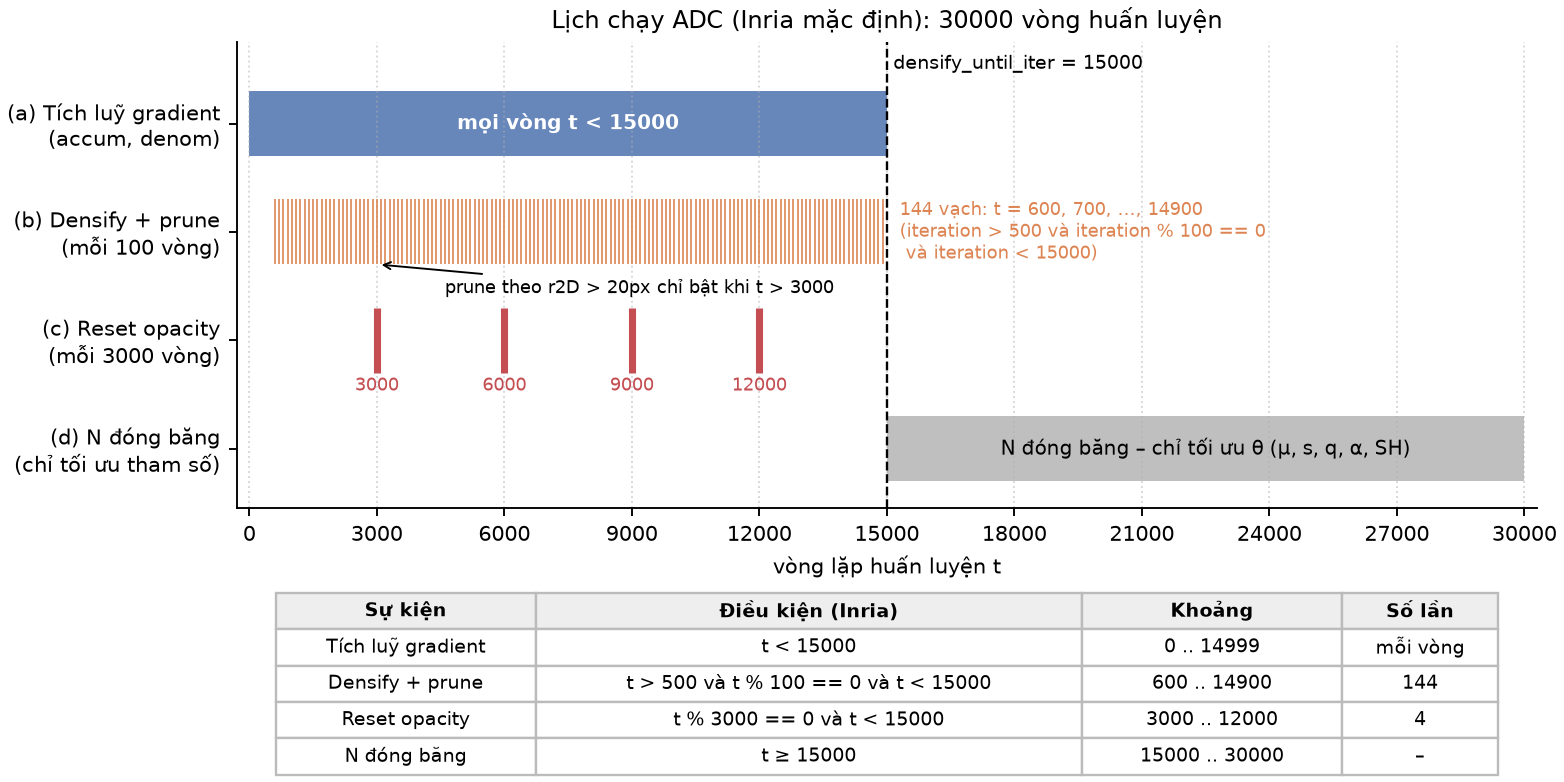
\includegraphics[width=0.62\linewidth]{fig_01_timeline.png}
\end{frame}

% --- Slide 33 ---
\begin{frame}{Tích luỹ gradient view-space}
\begin{columns}[T]
\begin{column}{0.52\textwidth}
\footnotesize
    \begin{itemize}
        \item Với mỗi Gaussian, gradient vị trí 2D (view-space) được \textbf{cộng dồn} qua nhiều lần render từ các camera khác nhau.
        \item Đồng thời đếm \texttt{denom}: số lần Gaussian đó thực sự được nhìn thấy (visible) trong batch.
        \item Gradient trung bình dùng làm tín hiệu quyết định densify:
        \[
            \bar{g} = \frac{\sum_{v} \nabla_{\text{view}} }{\text{denom}}
        \]
        \item $\bar g$ lớn $\Rightarrow$ ứng viên clone/split.
    \end{itemize}
\end{column}
\begin{column}{0.48\textwidth}
    \centering
    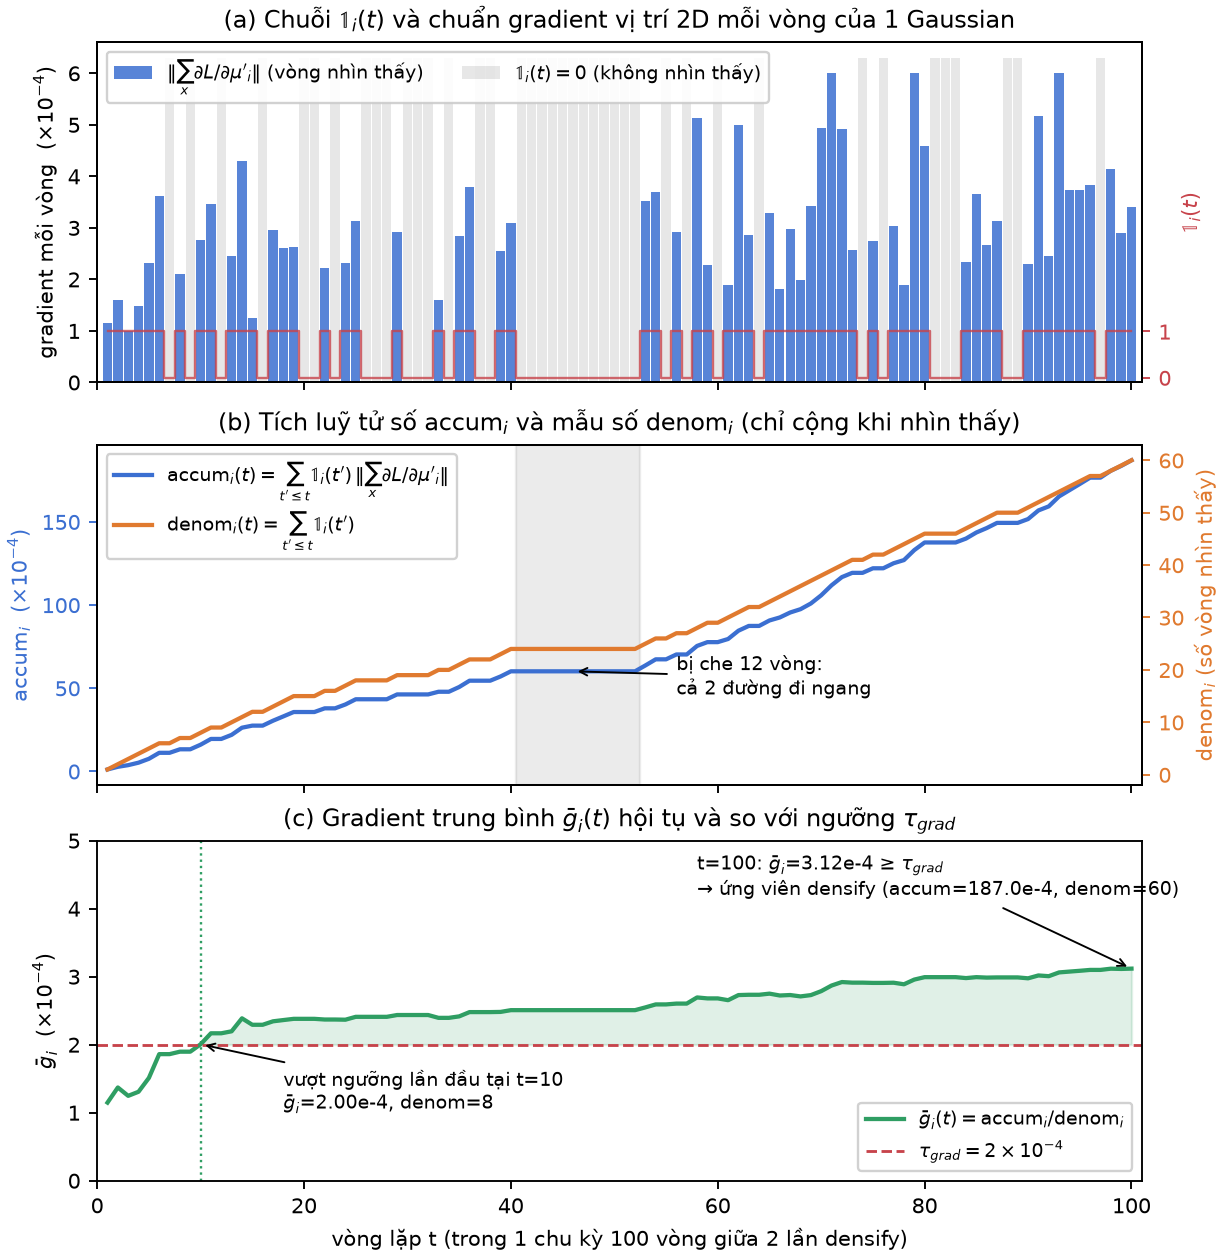
\includegraphics[width=0.95\linewidth]{fig_02_accum_denom.png}
\end{column}
\end{columns}
\end{frame}

% --- Slide 34 ---
\begin{frame}{Vấn đề triệt tiêu gradient (gradient cancellation)}
    \begin{itemize}
        \item Khi lấy trung bình vector gradient từ \textbf{nhiều view có hướng ngược nhau}, chúng có thể \textbf{triệt tiêu lẫn nhau}.
        \item Hệ quả: dù mỗi view riêng lẻ đều báo lỗi lớn (Gaussian sai vị trí/kích thước), $\bar g$ trung bình vẫn nhỏ $\Rightarrow$ Gaussian \textbf{bị bỏ sót}, không được densify.
        \item Đây là hạn chế đã biết của 3DGS gốc: chỉ dùng gradient trung bình làm tín hiệu duy nhất.
        \item FastGS cải thiện bằng \textbf{multi-view consistency score} thay vì chỉ dựa vào gradient trung bình (sẽ trình bày ở phần sau).
    \end{itemize}
    \vspace{0.2cm}
    \centering
    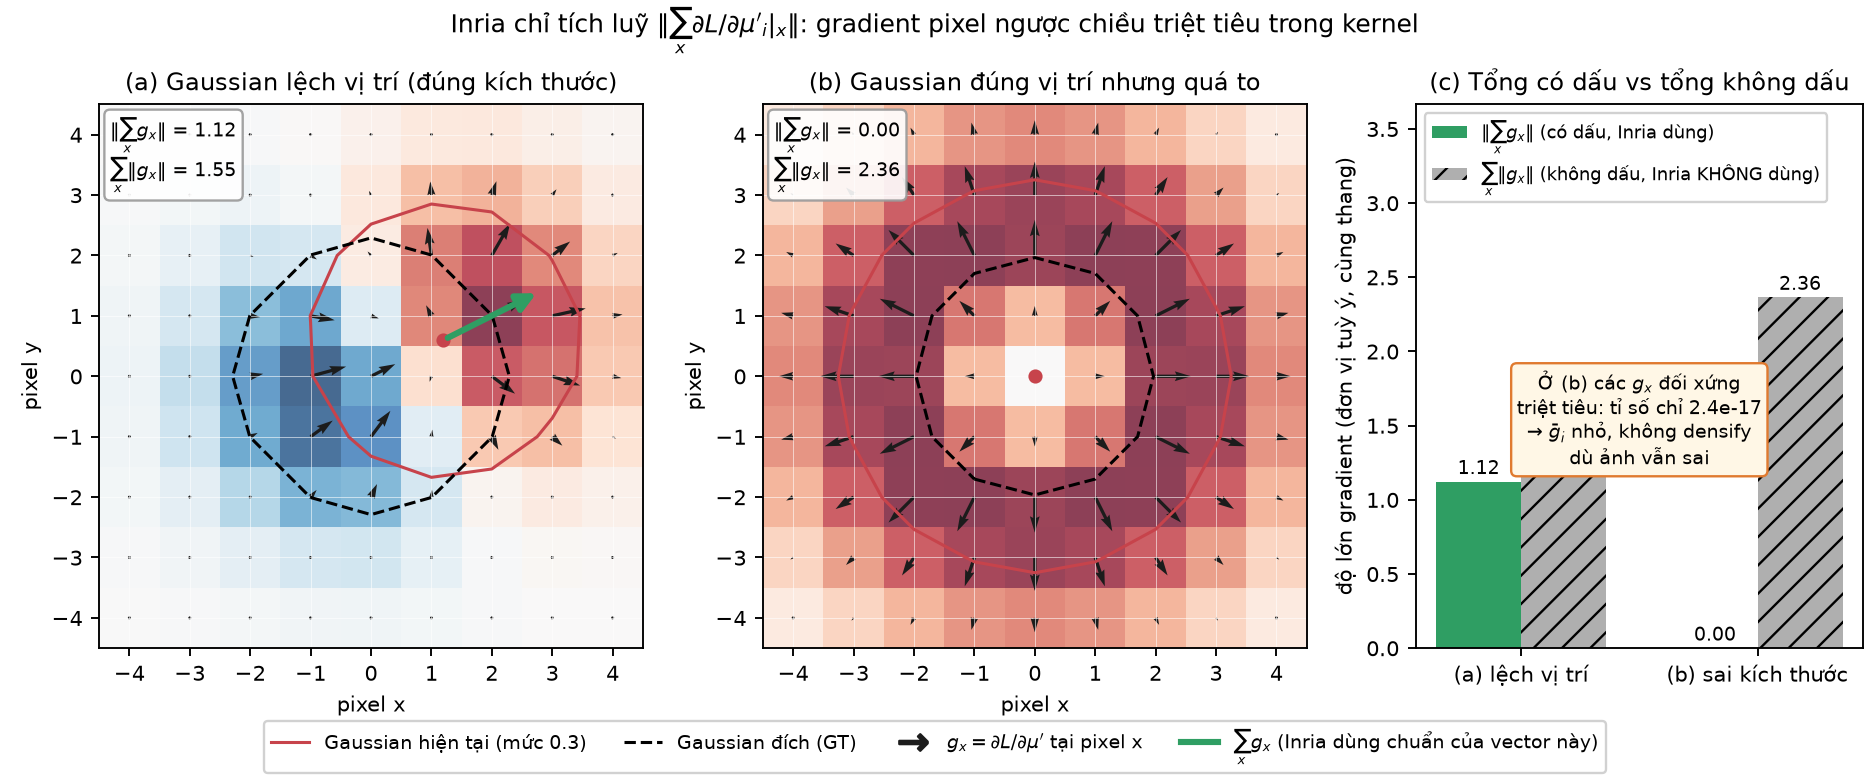
\includegraphics[width=0.75\linewidth]{fig_03_grad_cancel.png}
\end{frame}

% --- Slide 35 ---
\begin{frame}{Mặt phẳng quyết định clone/split}
\begin{columns}[T]
\begin{column}{0.52\textwidth}
\footnotesize
    \begin{itemize}
        \item \texttt{grad\_thresh} $= 0.0002$: ngưỡng gradient trung bình, kích hoạt \textbf{clone} nếu Gaussian nhỏ.
        \item \texttt{grad\_abs\_thresh} $= 0.0012$: ngưỡng absolute-gradient (kiểu Abs-GS), kích hoạt \textbf{split} nếu Gaussian lớn.
        \item Hai ngưỡng chia không gian (gradient, kích thước) thành 3 vùng: giữ nguyên / clone / split.
    \end{itemize}
\end{column}
\begin{column}{0.48\textwidth}
    \centering
    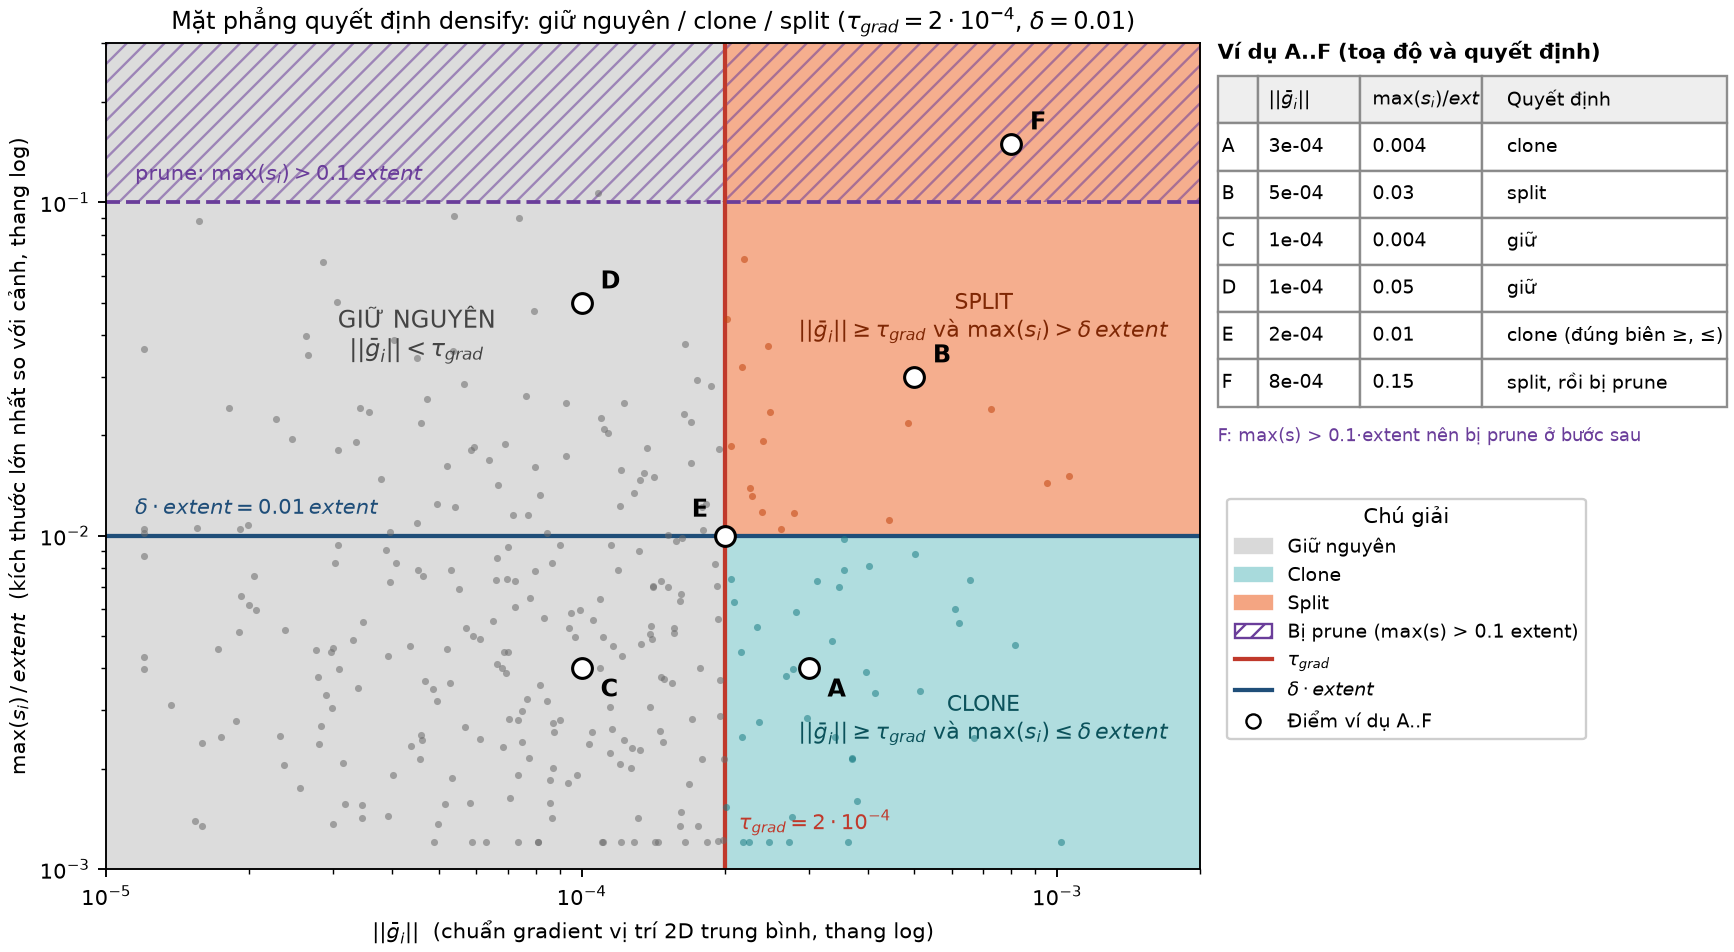
\includegraphics[width=0.95\linewidth]{fig_05_decision_plane.png}
\end{column}
\end{columns}
\end{frame}

% --- Slide 36 ---
\begin{frame}{Clone (nhân bản)}
    \footnotesize
    \begin{itemize}
        \item Áp dụng cho Gaussian \textbf{nhỏ nhưng thiếu hình học} (under-reconstruction).
        \item Nhân đôi Gaussian theo \textbf{hướng gradient vị trí} $\bar g$, đặt bản sao lệch một khoảng nhỏ.
        \item \textbf{Không} thay đổi kích thước/covariance -- chỉ lấp đầy vùng thiếu chi tiết bằng cách tăng mật độ.
    \end{itemize}
    \begin{columns}
        \begin{column}{0.48\linewidth}
            \centering
            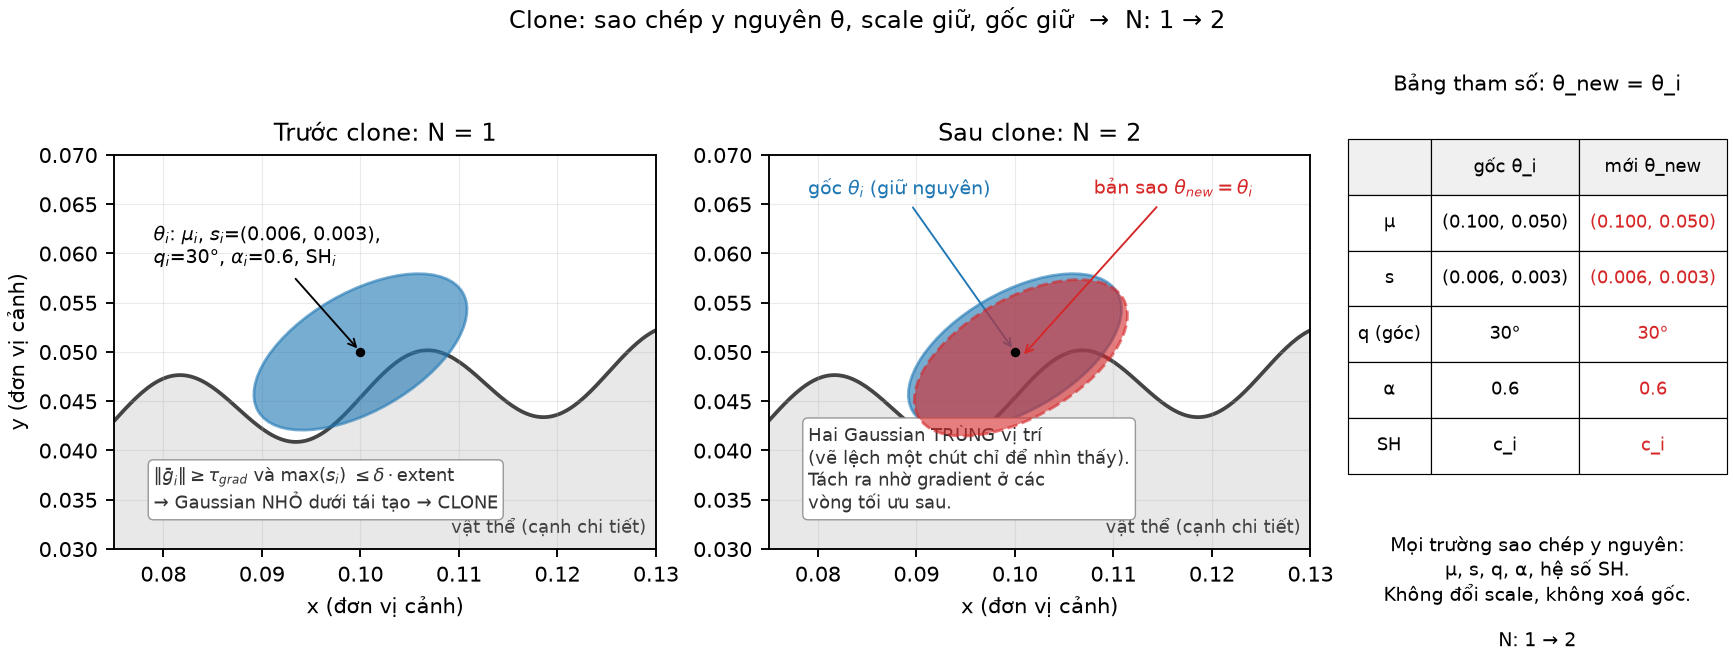
\includegraphics[width=\linewidth]{fig_08_clone_before_after.png}
            \captionof{figure}{Trước/sau clone}
        \end{column}
        \begin{column}{0.48\linewidth}
            \centering
            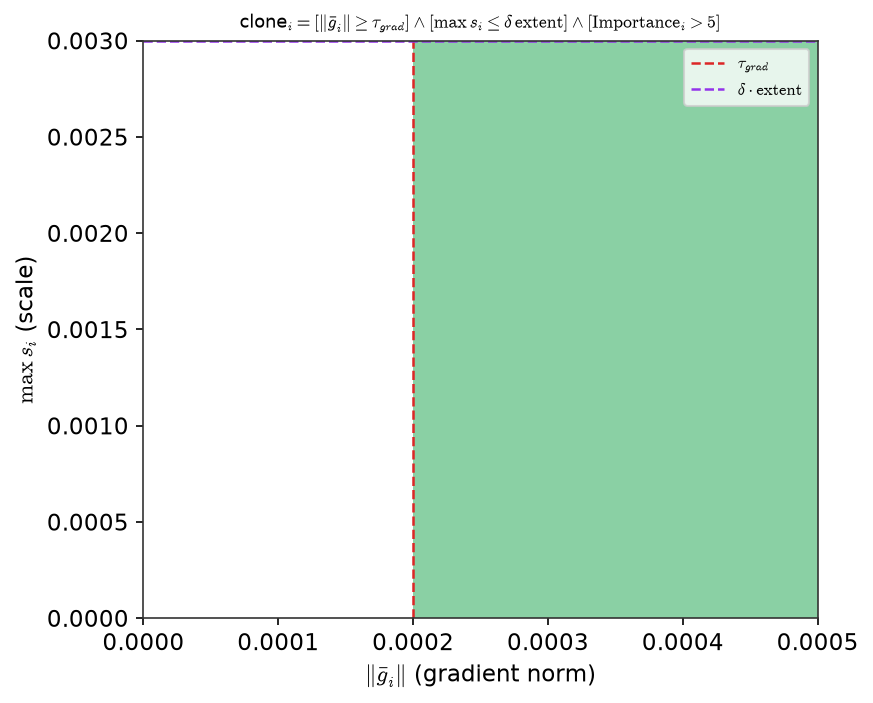
\includegraphics[width=\linewidth]{ch7_clone_region.png}
            \captionof{figure}{Vùng được clone}
        \end{column}
    \end{columns}
\end{frame}

% --- Slide 37 ---
\begin{frame}{Split (tách)}
    \footnotesize
    \begin{itemize}
        \item Áp dụng cho Gaussian \textbf{quá to} (over-reconstruction), vượt ngưỡng \texttt{--dense} theo scene extent.
        \item Tách thành \textbf{2 Gaussian con} nhỏ hơn (thường giảm scale theo hệ số cố định).
        \item Vị trí Gaussian con được \textbf{lấy mẫu ngẫu nhiên} theo phân phối chuẩn dựa trên chính covariance gốc của Gaussian cha.
    \end{itemize}
    \begin{columns}
        \begin{column}{0.48\linewidth}
            \centering
            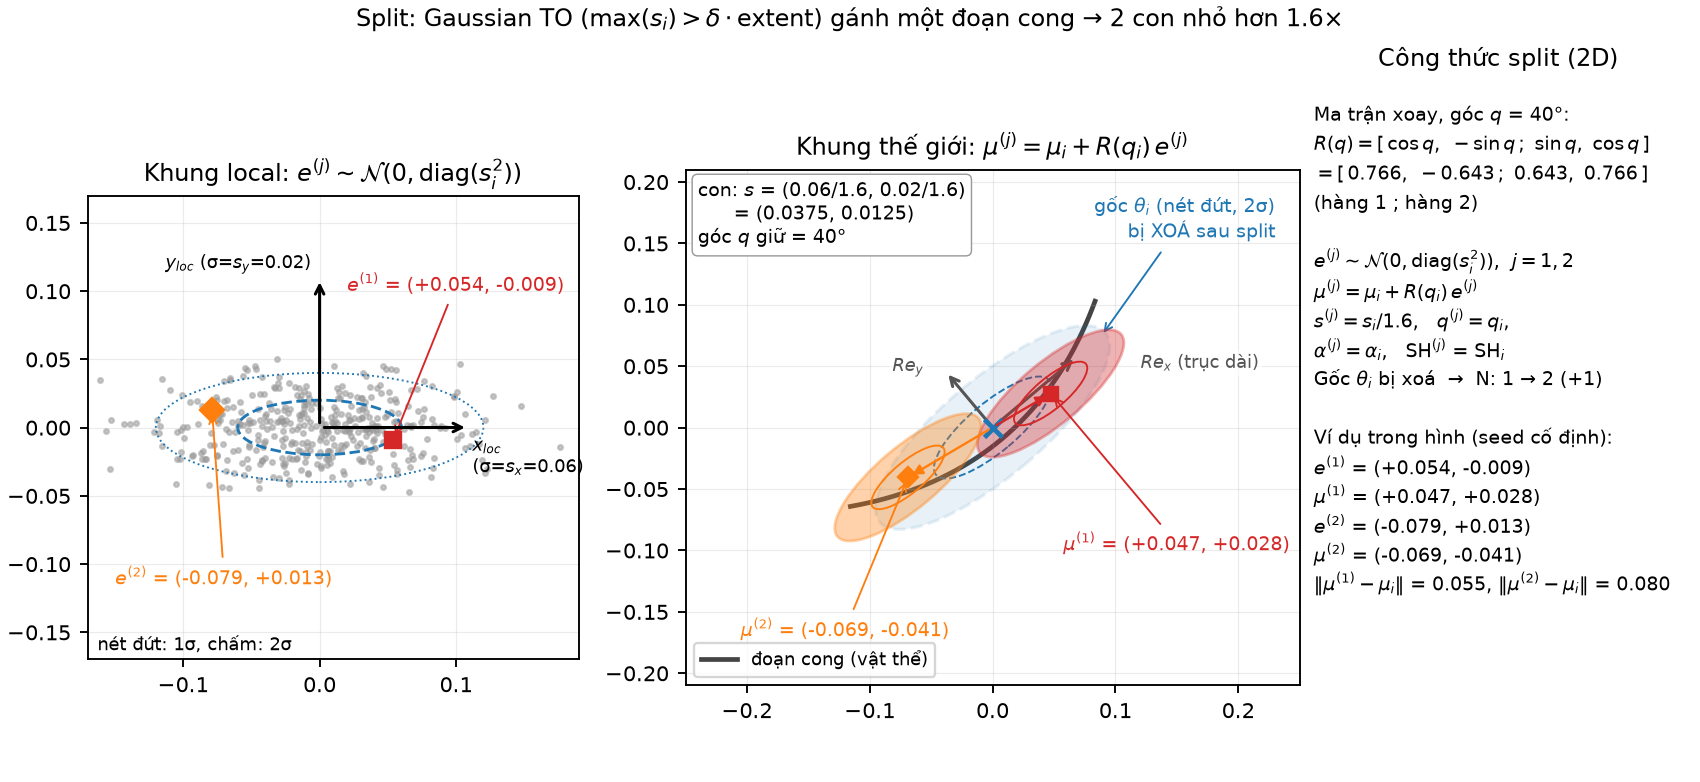
\includegraphics[width=\linewidth]{fig_09_split_geometry.png}
            \captionof{figure}{Hình học split}
        \end{column}
        \begin{column}{0.48\linewidth}
            \centering
            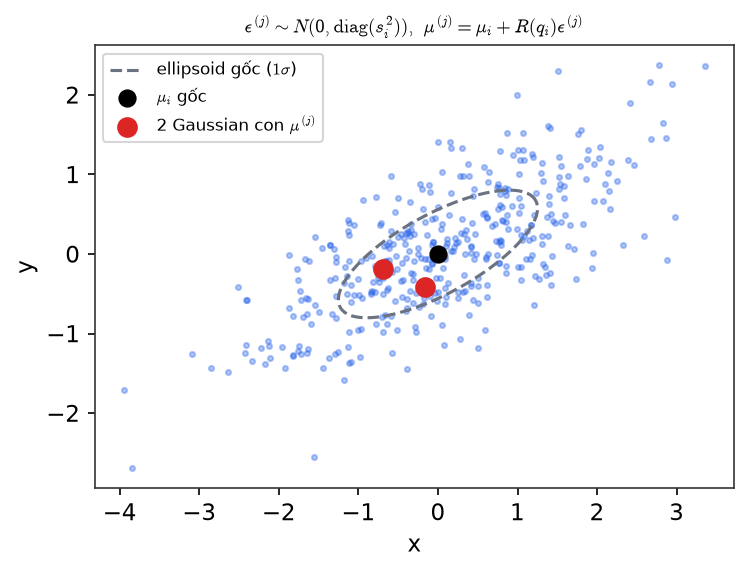
\includegraphics[width=\linewidth]{ch7_split_sampling.png}
            \captionof{figure}{Lấy mẫu theo covariance}
        \end{column}
    \end{columns}
\end{frame}

% --- Slide 38 ---
\begin{frame}{Prune theo độ quan trọng đa góc nhìn (FastGS)}
    \begin{itemize}
        \item 3DGS gốc: prune đơn thuần theo ngưỡng \textbf{opacity thấp} hoặc \textbf{kích thước quá lớn}.
        \item \textbf{FastGS}: tính điểm \emph{importance} cho mỗi Gaussian dựa trên đóng góp thực tế vào chất lượng ảnh render, tổng hợp qua \textbf{nhiều góc nhìn}.
        \item Gaussian có điểm importance thấp nhất bị cắt tỉa trước, bất kể opacity/kích thước.
        \item Kết quả: mô hình \textbf{gọn hơn} nhưng vẫn giữ chất lượng tái tạo -- đây là một đòn bẩy chính giúp FastGS tăng tốc.
    \end{itemize}
    \vspace{0.2cm}
    \centering
    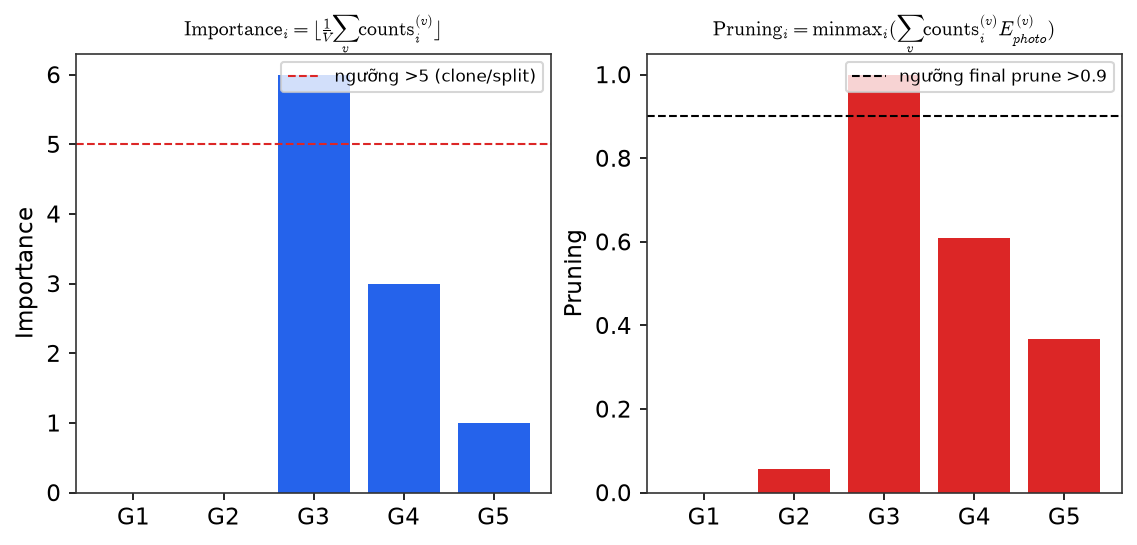
\includegraphics[width=0.7\linewidth]{ch7_importance_pruning.png}
\end{frame}

% --- Slide 39 ---
\begin{frame}{Số lượng Gaussian tăng theo iteration}
    \footnotesize
    \begin{itemize}
        \item Số Gaussian $N$ \textbf{tăng dần} qua mỗi vòng densify (clone + split).
        \item Có \textbf{bước nhảy rõ rệt} tại các mốc \texttt{densification\_interval}.
        \item $N$ \textbf{ngừng tăng} sau mốc \texttt{densify\_until\_iter}, chỉ còn giảm do prune.
    \end{itemize}
    \begin{columns}
        \begin{column}{0.48\linewidth}
            \centering
            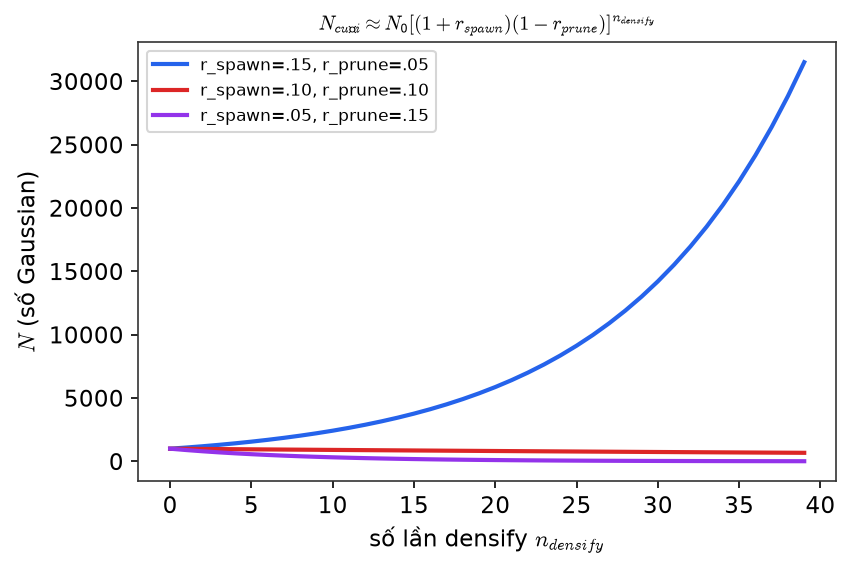
\includegraphics[width=\linewidth]{ch7_n_growth.png}
            \captionof{figure}{N tăng theo iteration}
        \end{column}
        \begin{column}{0.48\linewidth}
            \centering
            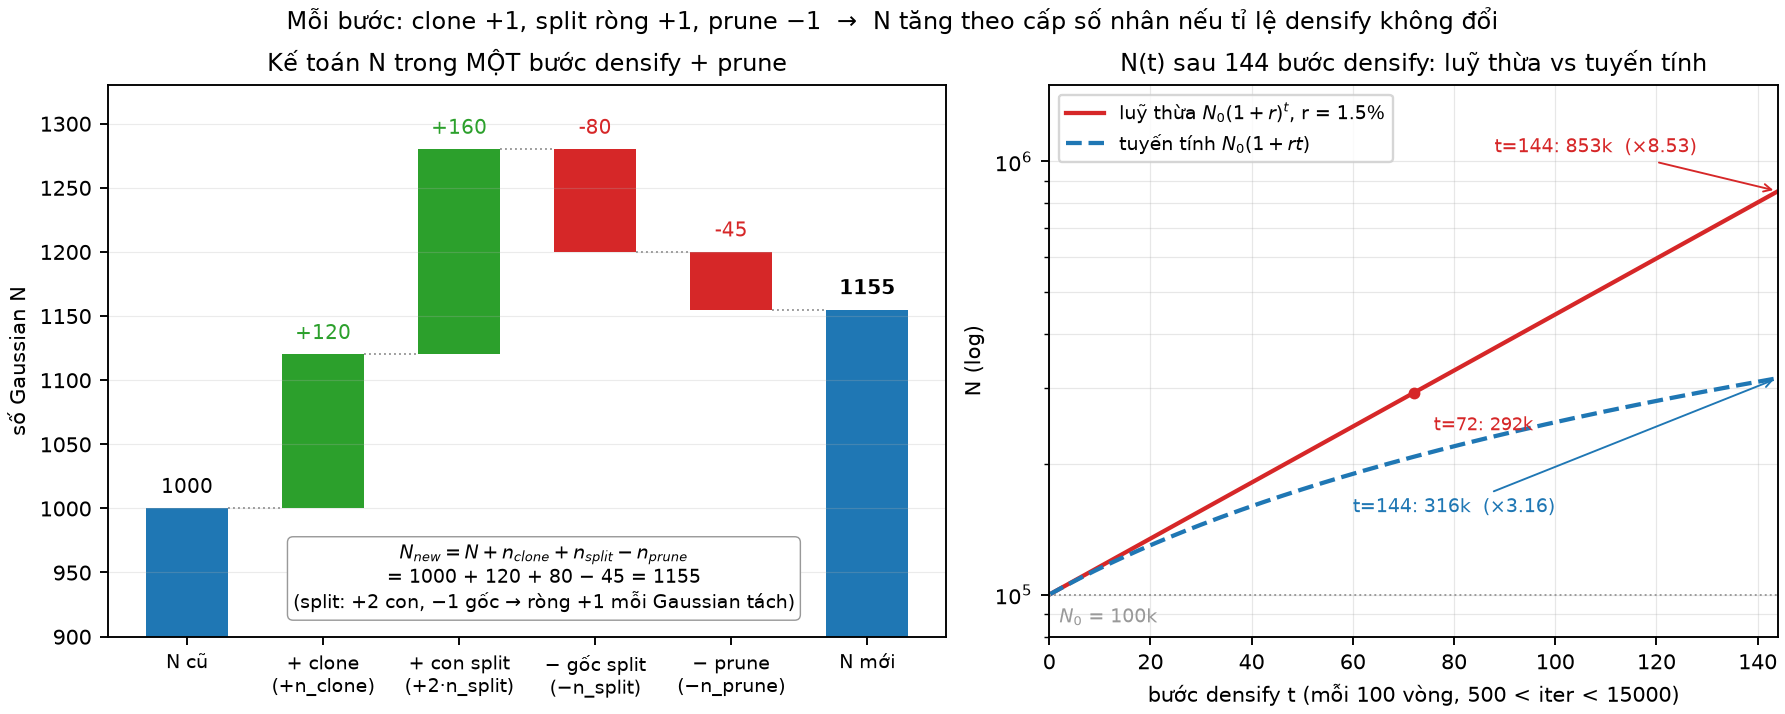
\includegraphics[width=\linewidth]{fig_11_N_accounting.png}
            \captionof{figure}{Hạch toán clone/split/prune}
        \end{column}
    \end{columns}
\end{frame}

% --- Slide 40 ---
\begin{frame}{Reset opacity định kỳ}
    \footnotesize
    \begin{itemize}
        \item Mỗi \texttt{opacity\_reset\_interval} (mặc định 3000 iteration): toàn bộ opacity được reset về \textbf{giá trị thấp} (qua sigmoid-inverse).
        \item Buộc optimizer \textbf{"đánh giá lại"} từng Gaussian từ đầu.
        \item Gaussian thực sự cần thiết: opacity \textbf{tăng trở lại} qua quá trình train.
        \item Gaussian dư thừa: opacity không hồi phục kịp $\Rightarrow$ bị \textbf{prune} ở vòng sau.
    \end{itemize}
    \begin{columns}
        \begin{column}{0.48\linewidth}
            \centering
            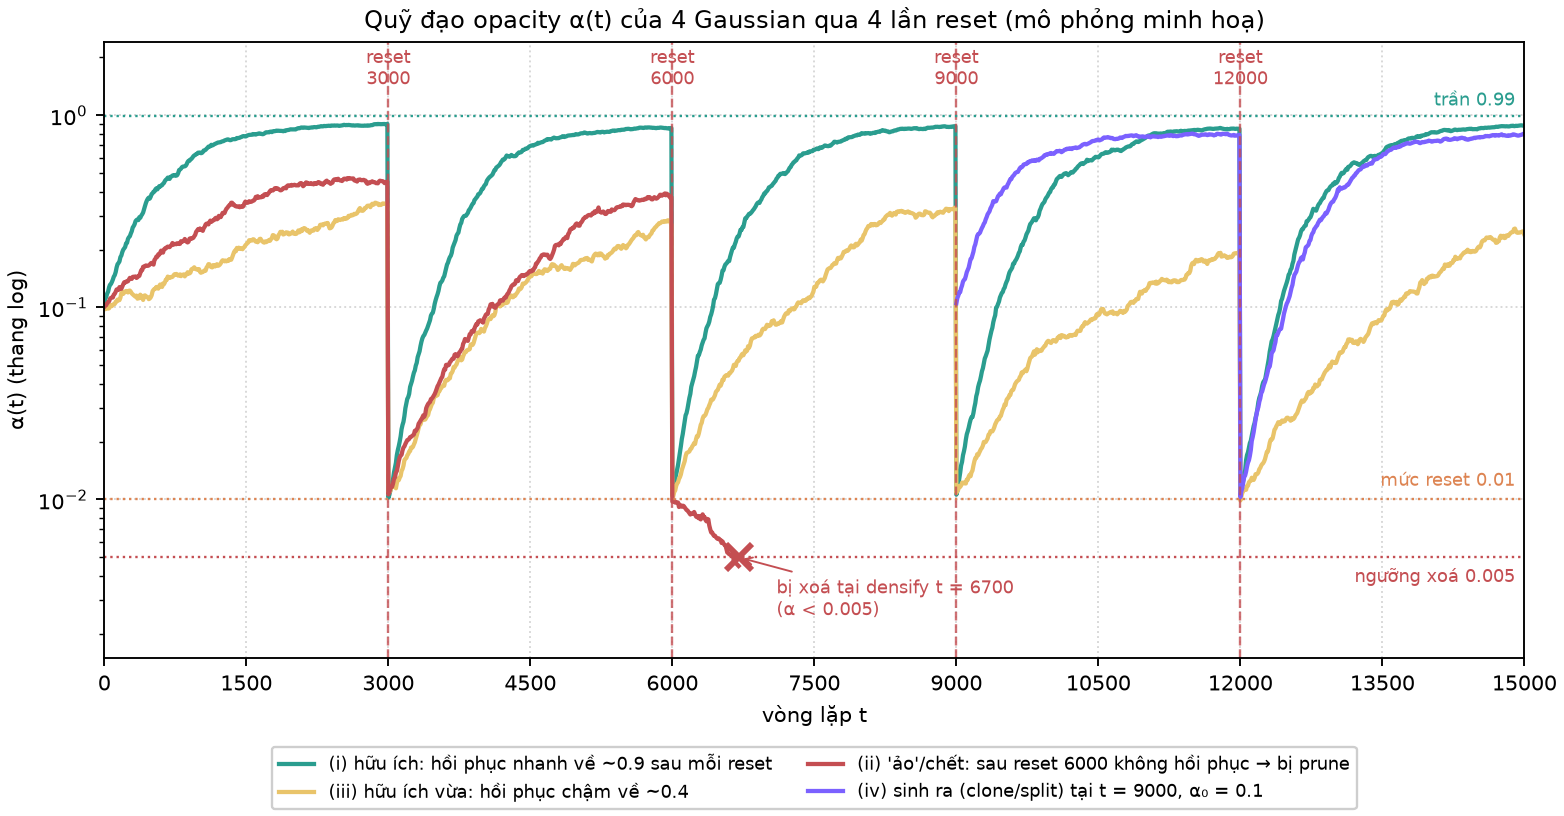
\includegraphics[width=\linewidth]{fig_17_opacity_trajectory.png}
            \captionof{figure}{Quỹ đạo opacity theo thời gian}
        \end{column}
        \begin{column}{0.48\linewidth}
            \centering
            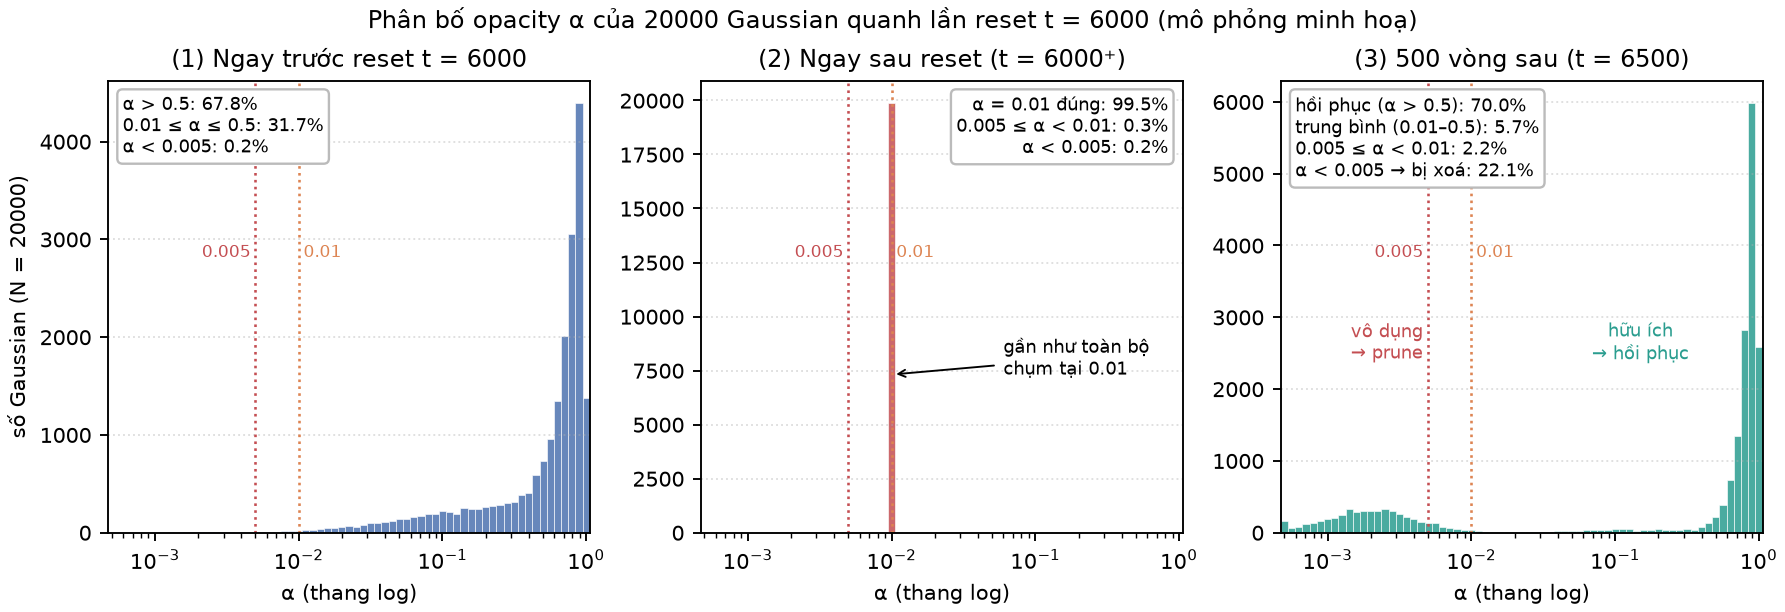
\includegraphics[width=\linewidth]{fig_18_hist_reset.png}
            \captionof{figure}{Histogram trước/sau reset}
        \end{column}
    \end{columns}
\end{frame}


% ===================== ADC CHUYÊN SÂU =====================
\section{ADC chuyên sâu — P1: Sai số ảnh \& tín hiệu pixel}
% === partADC_1a.tex ===
% Phan 1 (Section 1) cua chuong Adaptive Density Control (ADC) / FastGS-lite.
% Tin hieu sai so anh dung lam dau vao cho quyet dinh densify/prune,
% TRUOC khi tinh importance score da view.
% 6 frame, tuong ung 6 hinh trong DOCS/BOOK/adc_figures/part1_figures.py

% --- 1_1_timeline.png ---
\begin{frame}{Lịch chạy ADC trong vòng lặp huấn luyện (0 $\to$ 30000)}
\footnotesize
\begin{itemize}
    \item Adaptive Density Control không chạy liên tục: nó được \textbf{lồng} vào vòng lặp huấn luyện 30000 iteration theo các mốc cấu hình sẵn.
    \item \textbf{Tích luỹ thống kê gradient} (\texttt{accum}, \texttt{accum\_abs}, \texttt{denom}): chạy suốt $t < 15000$ (\texttt{densify\_until\_iter}).
    \item \textbf{Densify + prune}: từ $t = 500$ (\texttt{densify\_from\_iter}) đến $t = 15000$, lặp lại mỗi \texttt{densification\_interval} $= 500$ vòng $\Rightarrow$ 28 lần densify+prune (multinomial).
    \item \textbf{Reset opacity}: mỗi \texttt{opacity\_reset\_interval} $= 3000$ vòng, chỉ khi $t < 15000$ $\Rightarrow$ 4 lần tại $t = 3000, 6000, 9000, 12000$, đặt $\alpha \leftarrow \min(\alpha, 0.01)$.
    \item \textbf{Final prune} (đặc thù FastGS): mỗi 3000 vòng trong khoảng $15000 < t < 30000$ $\Rightarrow$ 4 lần tại $t = 18000, 21000, 24000, 27000$, xoá thẳng Gaussian có $\alpha < 0.1$ \textbf{hoặc} điểm Pruning $> 0.9$.
    \item Sau $t = 30000$: kết thúc huấn luyện, \textbf{không} còn final prune nào nữa.
\end{itemize}
\begin{center}
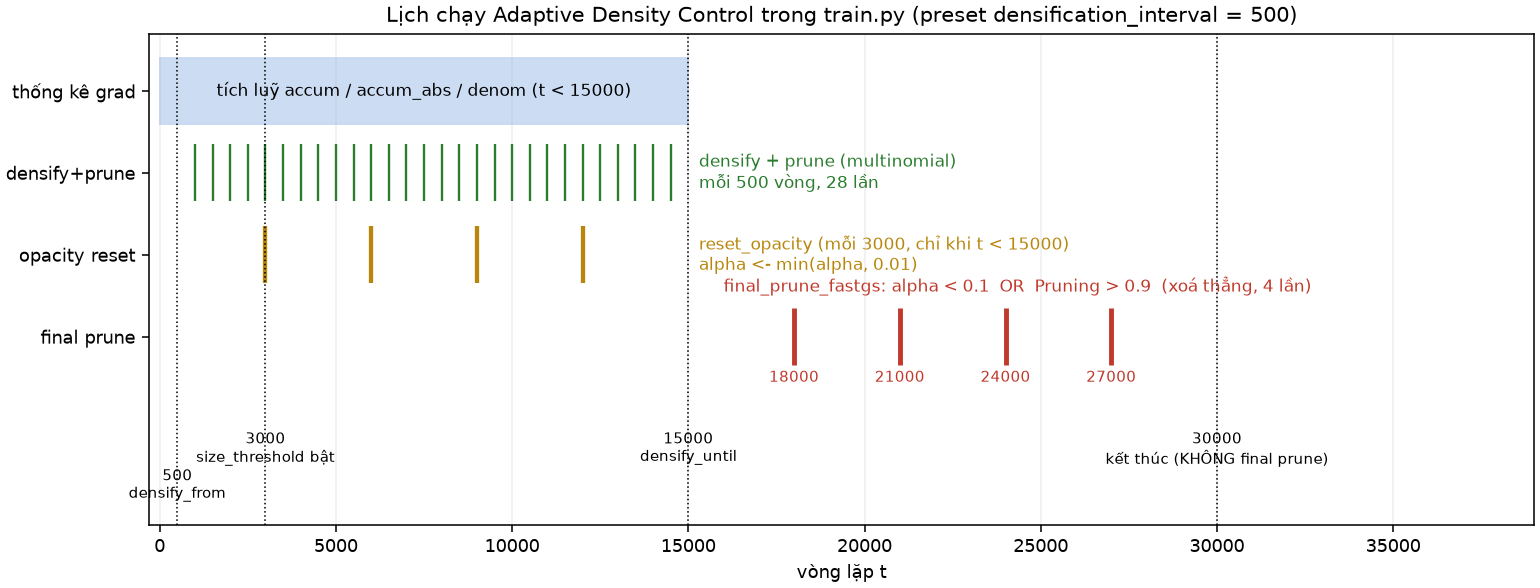
\includegraphics[width=0.78\linewidth]{1_1_timeline.png}
\captionof{figure}{\footnotesize Lịch chạy ADC trong \texttt{train.py} với preset \texttt{densification\_interval} $= 500$: 4 dải mốc — thống kê gradient, densify+prune, reset opacity, final prune.}
\end{center}
\end{frame}

% --- 1_2_N_qualitative.png ---
\begin{frame}{Số lượng Gaussian $N(t)$ thay đổi ra sao qua các giai đoạn}
\begin{columns}[T]
\begin{column}{0.52\linewidth}
\footnotesize
\begin{itemize}
    \item Mỗi lần densify là một \textbf{phép nhân}, không phải phép cộng: sau mỗi bước tại $t \in (500, 15000)$,
    \[
        N \leftarrow N \cdot (1 + r_{\text{spawn}}) \cdot (1 - r_{\text{prune}}).
    \]
    \item Vì lặp lại 28 lần, chênh lệch nhỏ ở $r_{\text{spawn}}$ tạo tác động \textbf{luỹ thừa} lên $N$ cuối giai đoạn densify.
    \item 3DGS gốc: $r_{\text{spawn}} \approx 0.085$, $r_{\text{prune}} \approx 0.035$, không có final prune $\Rightarrow N$ tăng nhanh rồi giữ nguyên.
    \item FastGS-lite: $r_{\text{spawn}} \approx 0.045$ (chọn lọc hơn nhờ điều kiện Importance $> 5$), cộng thêm final prune với $r_{\text{final}} \approx 0.12$ mỗi 3000 vòng trong $(15000, 30000)$.
    \item Kết quả định tính: $N$ \textbf{tăng nhanh} đầu train, \textbf{chững lại} khi hết giai đoạn densify ($t=15000$), rồi \textbf{giảm bậc thang} tại mỗi lần final prune.
\end{itemize}
\end{column}
\begin{column}{0.46\linewidth}
\centering
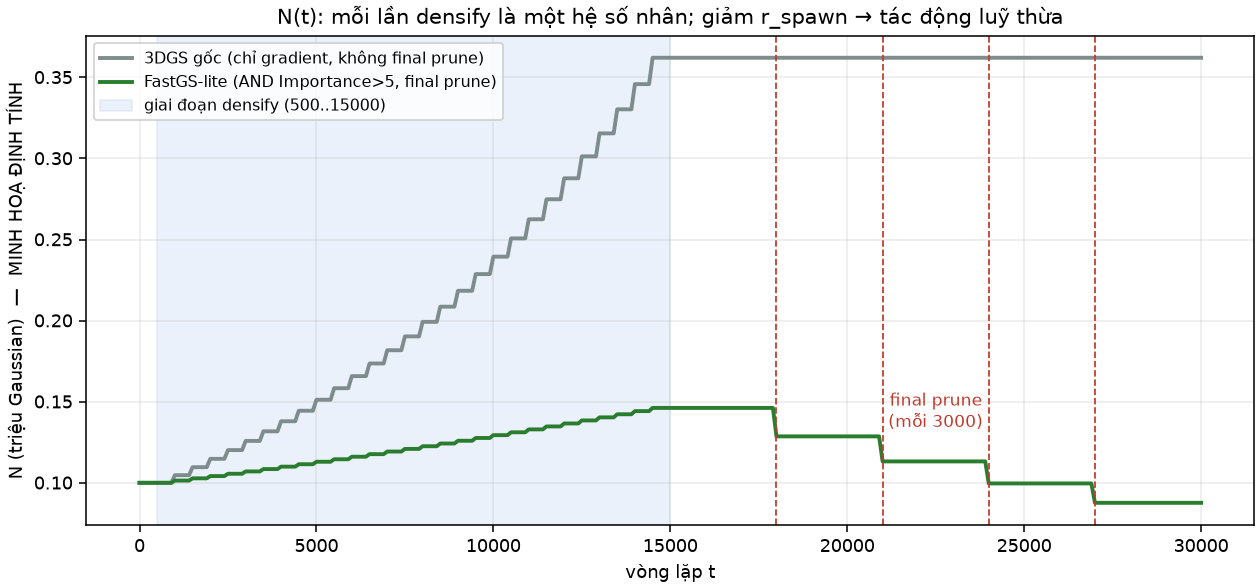
\includegraphics[width=\linewidth]{1_2_N_qualitative.png}
\captionof{figure}{\footnotesize $N(t)$ minh hoạ định tính: 3DGS gốc (xám) chỉ tăng rồi bão hoà; FastGS-lite (xanh) có thêm các bậc giảm do final prune mỗi 3000 vòng.}
\end{column}
\end{columns}
\end{frame}

% --- 1_3_pixel_error_view1.png ---
\begin{frame}{Bước (1): sai số ảnh theo từng pixel $e_v(x)$}
\begin{columns}[T]
\begin{column}{0.5\textwidth}
\scriptsize
\begin{itemize}
    \item Đầu vào: ảnh render $I_{\text{rend}}$ và ground truth $I_{\text{gt}}$ tại view $v$, mỗi ảnh 3 kênh màu.
    \item Sai số pixel (chuẩn $L_1$ trung bình theo kênh):
    $\displaystyle e_v(x) = \frac{1}{3}\sum_{c} \left| I_{\text{rend}}^{c}(x) - I_{\text{gt}}^{c}(x) \right|$.
    \item Ví dụ lưới $4{\times}4$: $e_v(P_7){=}\frac{0.30+0.24+0.21}{3}{=}0.25$, nền chỉ ${\approx}0.01$--$0.02$.
    \item Cả lưới cho $e_v{\in}[0.01,0.40]$: vùng $P7,P8,P11,P12,P15,P16$ sai số lớn — "bản đồ lỗi" thô chuẩn hoá ở bước (2).
\end{itemize}
\end{column}
\begin{column}{0.5\textwidth}
\centering
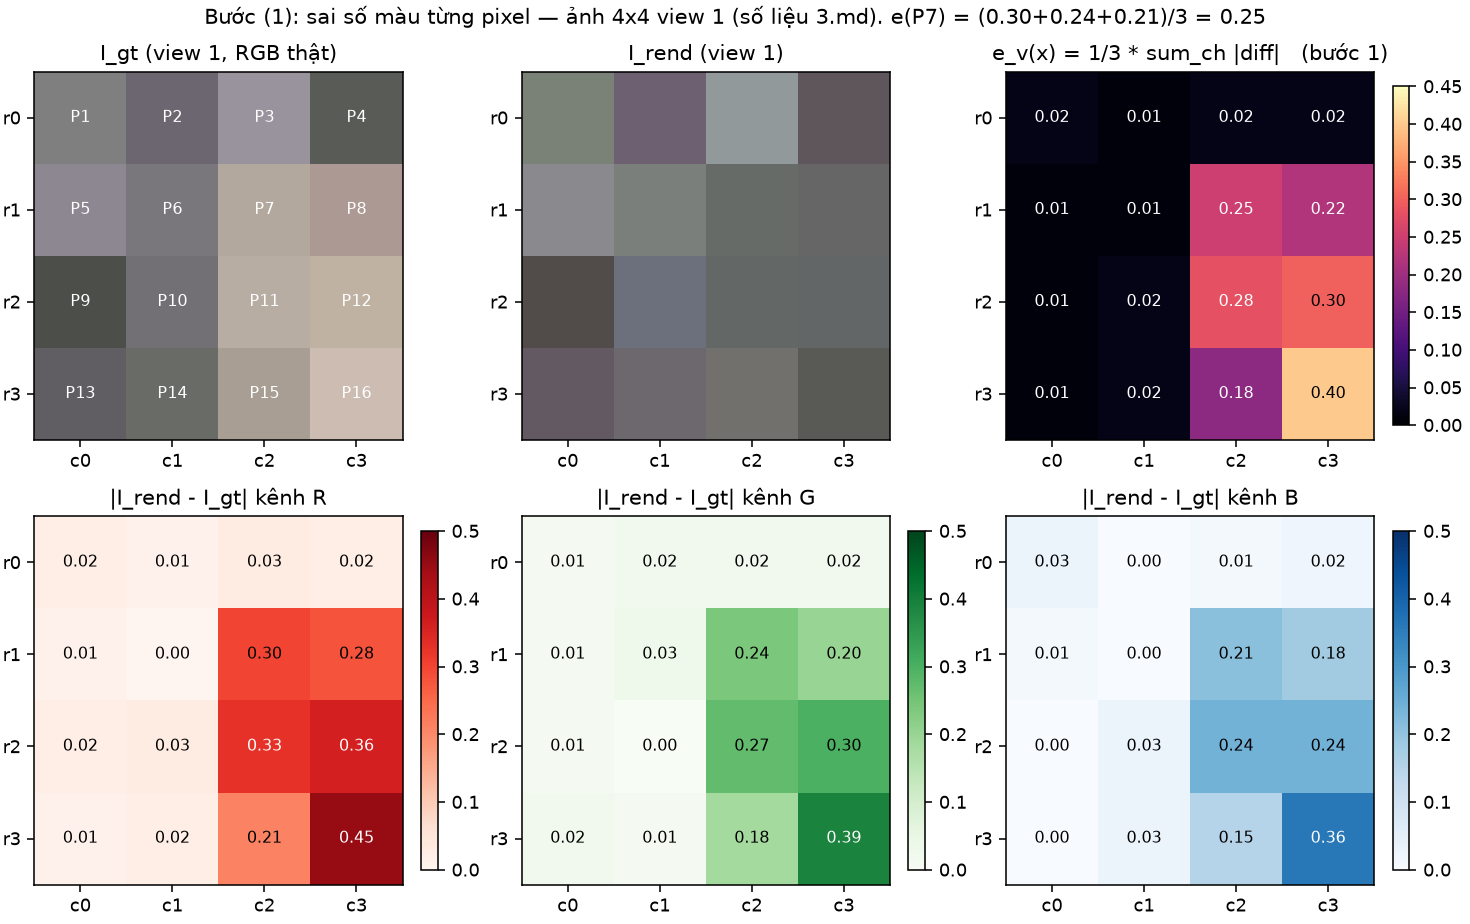
\includegraphics[width=0.95\linewidth]{1_3_pixel_error_view1.png}
\captionof{figure}{\footnotesize $I_{\text{gt}}$, $I_{\text{rend}}$, bản đồ $e_v(x)$ trên lưới $4\times4$.}
\end{column}
\end{columns}
\end{frame}

% --- 1_4_l1_vs_l2.png ---
\begin{frame}{Vì sao dùng $L_1$ thay vì $L_2$ ở bước (1)}
\begin{columns}[T]
\begin{column}{0.52\linewidth}
\footnotesize
\begin{itemize}
    \item Với $d = |I_{\text{rend}} - I_{\text{gt}}|$ trên một kênh, hai lựa chọn đóng góp vào $e_v(x)$:
    \[
        L_1: \; d, \qquad L_2 \text{ (không căn)}: \; d^2.
    \]
    \item Với sai số nhỏ $d = 0.05$: $L_1 = 0.05$ nhưng $d^2 = 0.0025$ — $L_2$ "bóp" gần như triệt tiêu các lệch màu nhỏ, còn $L_1$ giữ tuyến tính.
    \item Ngược lại, với sai số lớn (vùng vật thể chuyển động, $d \approx 0.3$--$0.4$), $d^2$ phóng đại mạnh hơn nhiều so với $d$ $\Rightarrow$ $L_2$ nhạy outlier hơn.
    \item Trên 16 pixel ví dụ, tỉ lệ $\max(e)/\text{median}(e)$ (đo "đuôi dài" của phân phối) của MSE cao hơn hẳn so với $L_1$ trên thang log.
    \item Vì bước (2) sẽ chuẩn hoá theo $\min/\max$ của toàn ảnh, dùng $L_1$ ở bước (1) giúp bản đồ lỗi ổn định hơn trước khi bị outlier chi phối thêm lần nữa.
\end{itemize}
\end{column}
\begin{column}{0.46\linewidth}
\centering
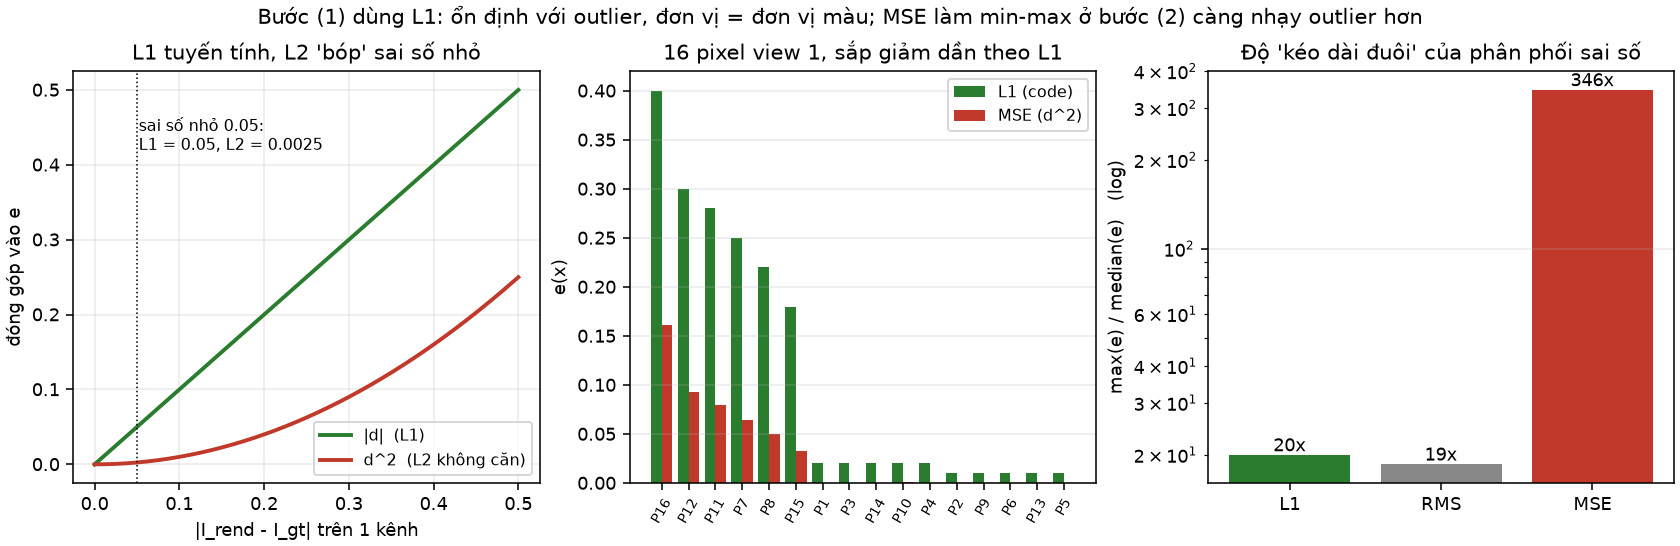
\includegraphics[width=\linewidth]{1_4_l1_vs_l2.png}
\captionof{figure}{\footnotesize So sánh $L_1$ ($|d|$, tuyến tính) và $L_2$ ($d^2$, phạt nặng outlier) trên cùng bộ 16 pixel view 1.}
\end{column}
\end{columns}
\end{frame}

% --- 1_5_minmax_3views.png ---
\begin{frame}{Bước (2): chuẩn hoá min-max trên từng ảnh}
\scriptsize
\begin{itemize}
    \item Mỗi view $v$ chuẩn hoá độc lập theo $\min,\max$ của chính $e_v$ trên ảnh đó:
    $\displaystyle \tilde{e}_v(x) = \frac{e_v(x) - \min_x e_v(x)}{\max_x e_v(x) - \min_x e_v(x)} \in [0,1]$.
    \item Ba view khác hẳn nhau: view 1 "tệ" ($e_v{\in}[0.01,0.40]$), view 2 "tốt" ($[0.01,0.16]$), view 3 trung bình ($[0.01,0.24]$).
    \item Sau chuẩn hoá, cả ba dùng \textbf{chung ngưỡng} $\tau_{\text{loss}}{=}0.1$ ở bước (3).
    \item Ngưỡng tuyệt đối tương đương khác nhau theo view: view 1 là $e_v{>}0.049$, view 2 là $e_v{>}0.025$, view 3 là $e_v{>}0.033$ — view "tốt" và "tệ" cho số pixel bật tương đương về mặt \emph{tương đối}.
\end{itemize}
\centering
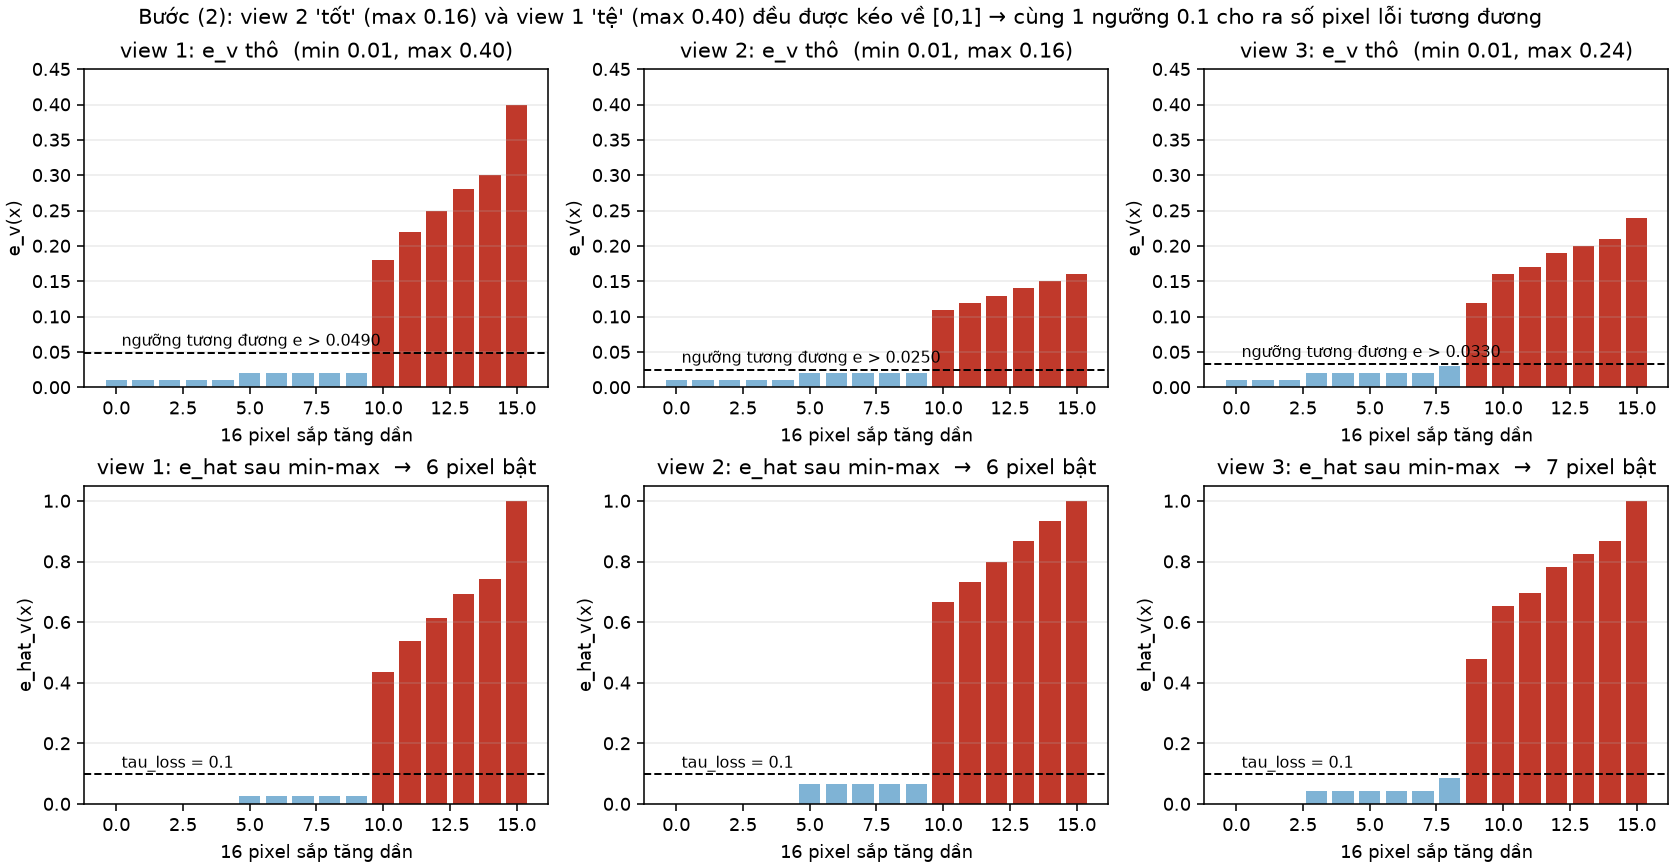
\includegraphics[width=0.62\linewidth]{1_5_minmax_3views.png}
\captionof{figure}{\footnotesize $e_v$ thô (trên) và $\tilde{e}_v$ sau min-max (dưới), 3 view; nét đứt = $\tau_{\text{loss}}=0.1$.}
\end{frame}

% --- 1_6_outlier.png ---
\begin{frame}{Vấn đề của min-max: một outlier bóp méo toàn bộ thang đo}
\begin{columns}[T]
\begin{column}{0.52\linewidth}
\footnotesize
\begin{itemize}
    \item Chuẩn hoá min-max chỉ phụ thuộc \textbf{duy nhất} vào hai giá trị $\min$ và $\max$ của cả ảnh $\Rightarrow$ rất nhạy với một điểm bất thường.
    \item Ví dụ: giữ nguyên lưới $4\times4$ view 1 nhưng đặt $e_v(P_1) = 0.90$ (mô phỏng một pixel lỗi/vật thể chuyển động đột ngột).
    \item Mẫu số $(\max - \min)$ tăng từ $0.39$ ($0.40 - 0.01$) lên $0.89$ ($0.90 - 0.01$) $\Rightarrow$ ngưỡng tuyệt đối tương đương tăng từ $0.049$ lên $0.099$.
    \item Hệ quả: các pixel lỗi thật sự khác (ví dụ $P_7$--$P_{16}$) bị \textbf{"nén"} giá trị $\tilde{e}_v$ xuống gần một nửa, dù bản chất sai số của chúng không đổi.
    \item $P_{15}$ ($e_v = 0.18$) vẫn còn bật ($\tilde{e}_v = 0.191 > 0.1$), nhưng biên an toàn bị thu hẹp đáng kể — chỉ cần thêm vài outlier là toàn bộ importance của các Gaussian khác trong ảnh bị méo theo.
\end{itemize}
\end{column}
\begin{column}{0.46\linewidth}
\centering
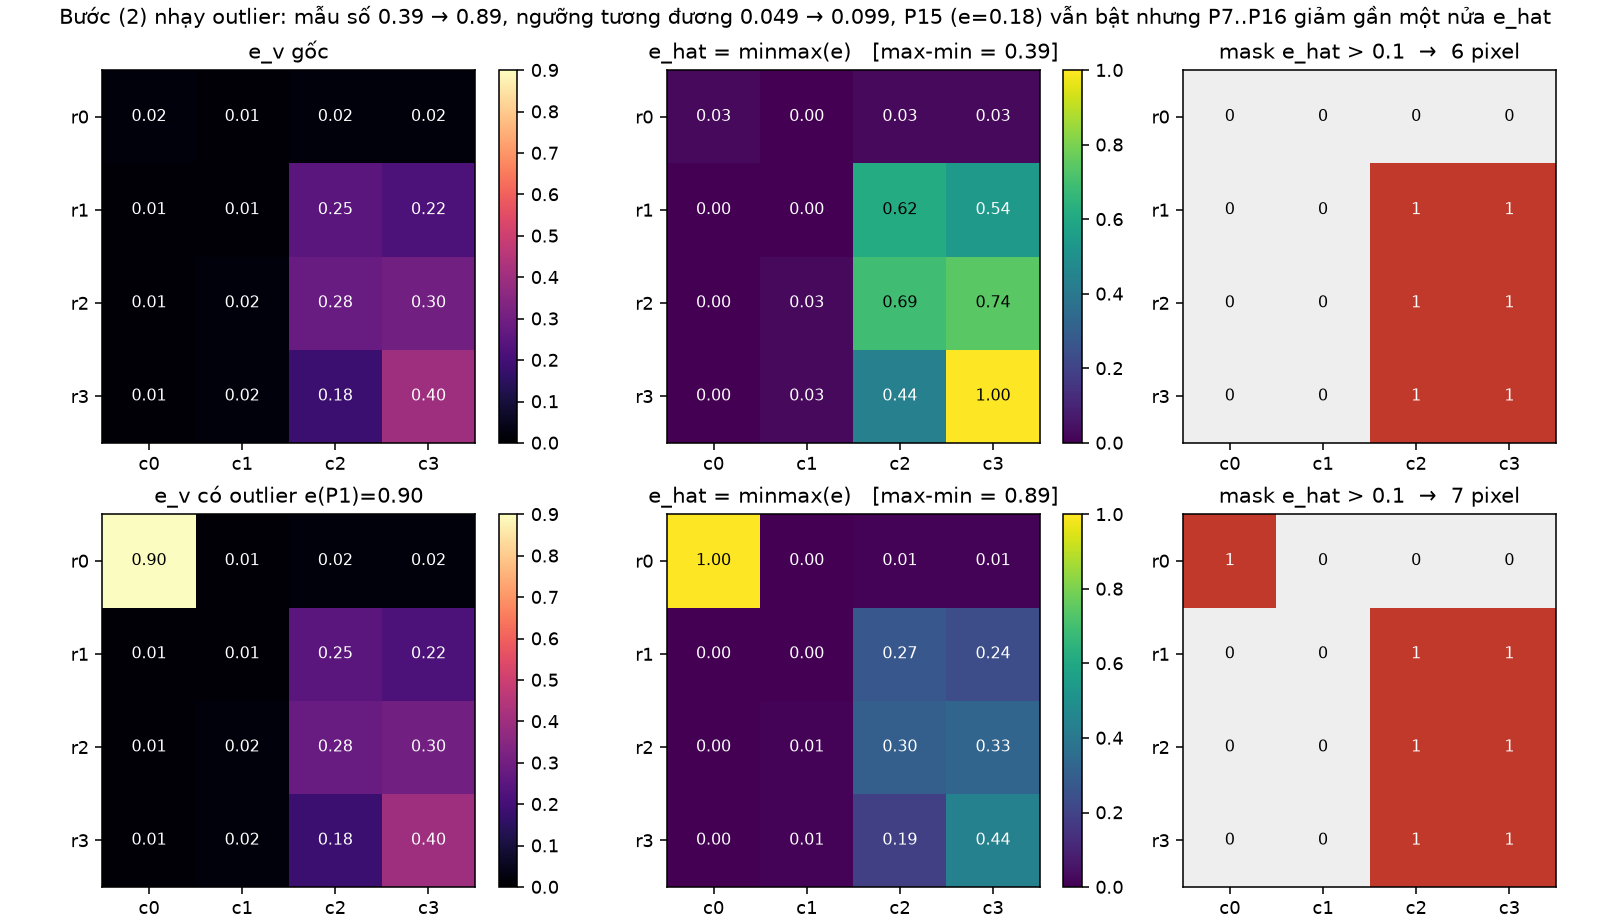
\includegraphics[width=\linewidth]{1_6_outlier.png}
\captionof{figure}{\footnotesize So sánh $e_v$, $\tilde{e}_v$ và mặt nạ $\tilde{e}_v > 0.1$ trước/sau khi thêm một outlier duy nhất ($e_v(P_1){=}0.90$).}
\end{column}
\end{columns}
\end{frame}

% partADC_1b.tex --- ADC-1b: Ngưỡng hoá (thresholding) và cài đặt PyTorch
% Tiếp nối ADC-1a (chuẩn hoá sai số). KHÔNG chứa \documentclass/\usepackage/\begin{document}.

% --- 1_7_norm_compare.png ---
\begin{frame}{Bước (2): vì sao chọn min-max thay vì z-score/percentile?}
\begin{columns}[T]
\begin{column}{0.48\linewidth}
\footnotesize
\begin{itemize}
\item Bản đồ sai số mô phỏng $48\times32$: nền thấp $\approx 0.01$--$0.02$, hai vùng lỗi cục bộ (Gaussian), và \textbf{một outlier đơn lẻ} tại pixel $(3,44)$ với $e=0.95$.
\item Min-max: $\tilde e = \dfrac{e - e_{\min}}{e_{\max} - e_{\min}}$ — chỉ phụ thuộc \textbf{duy nhất} vào $e_{\min}, e_{\max}$ của toàn ảnh.
\item Z-score: $z = \dfrac{e - \mu}{\sigma}$, rồi co về $[0,1]$ — là biến đổi \textbf{affine}, nên \textbf{cùng thứ tự xếp hạng pixel} với min-max.
\item Percentile 5--95: $\mathrm{clip}\!\left(\dfrac{e-p_5}{p_{95}-p_5},0,1\right)$ — bền với outlier hơn (outlier bị clip) nhưng tốn thêm một lần \texttt{sort}/\texttt{quantile}.
\item Kết luận code FastGS: min-max \textbf{rẻ} (chỉ cần \texttt{min}/\texttt{max}), đủ tốt cho mục đích so sánh tương đối giữa các pixel trong cùng một view.
\end{itemize}
\end{column}
\begin{column}{0.48\linewidth}
\centering
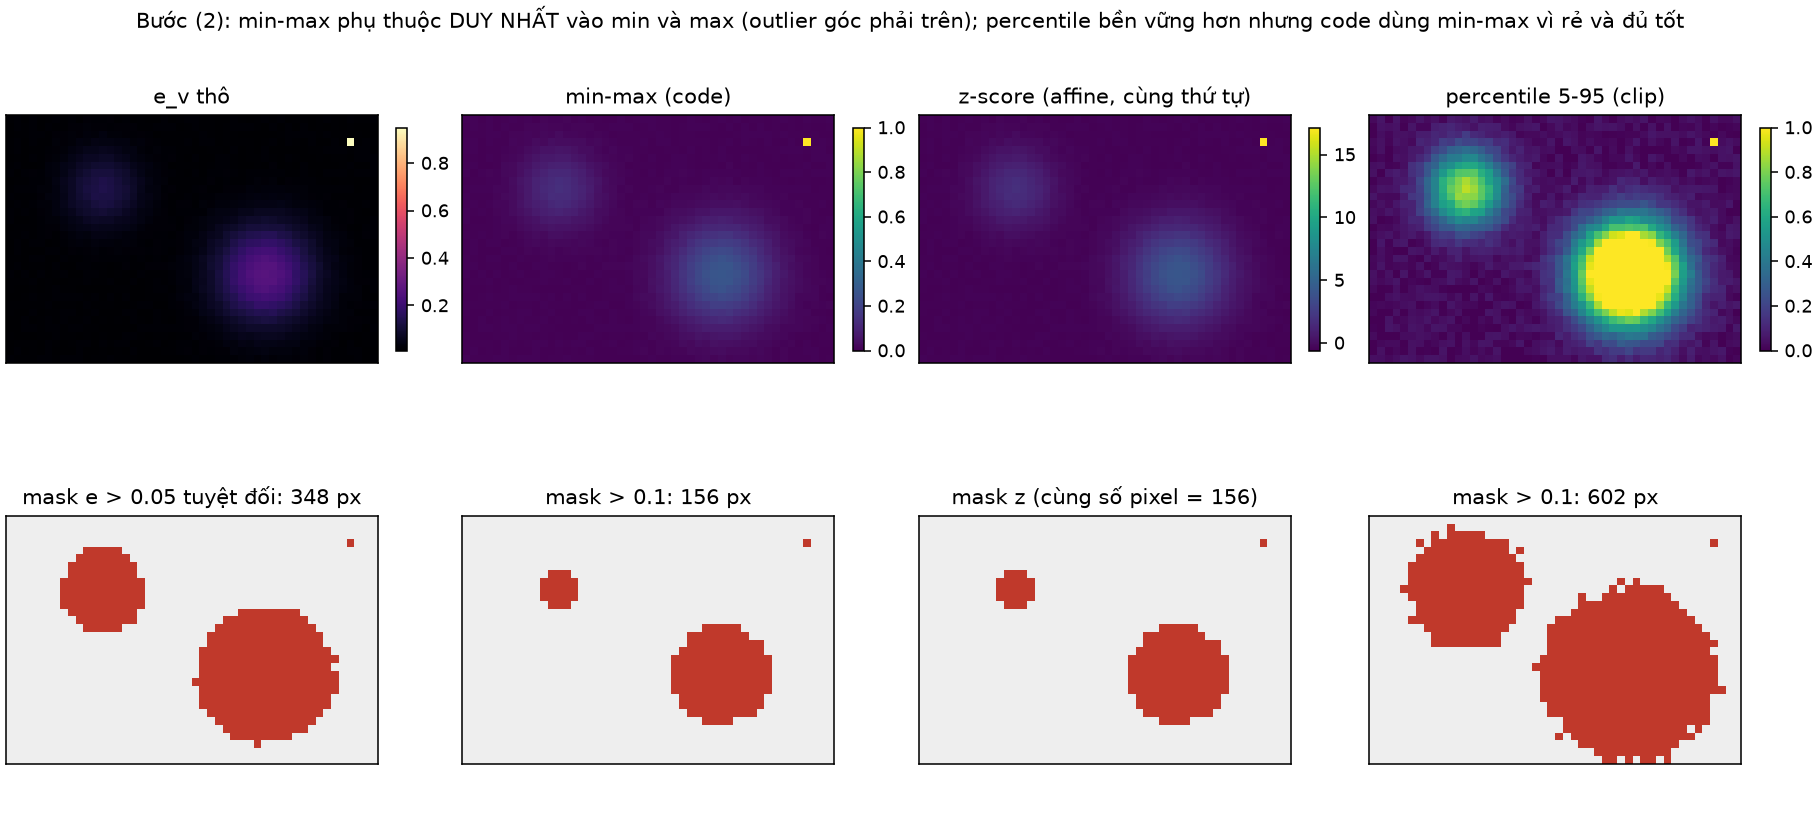
\includegraphics[width=0.98\linewidth]{1_7_norm_compare.png}
\captionof{figure}{\footnotesize So sánh $e_v$ thô, min-max, z-score (cùng thứ tự với min-max), và percentile 5--95 (clip outlier) trên cùng bản đồ sai số.}
\end{column}
\end{columns}
\end{frame}

% --- 1_8_tau_masks.png ---
\begin{frame}{Bước (3): mặt nạ nhị phân với $\tau_{\text{loss}} = 0.1$}
\begin{columns}[T]
\begin{column}{0.5\textwidth}
\scriptsize
\begin{itemize}
\item Mặt nạ lỗi cao: $m_v(x) = \mathbb{1}[\tilde e_v(x) > \tau_{\text{loss}}]$, $\tau_{\text{loss}}{=}0.1$.
\item Quét $\tau{\in}\{0.05,0.1,0.2,0.5\}$ trên 3 view $4{\times}4$: số pixel bật giảm dần khi $\tau$ tăng.
\item Với $\tau_{\text{loss}}{=}0.1$: mặt nạ tách sạch "nền" và "lỗi" — không quá thưa ($\tau{=}0.5$) hay quá dày ($\tau{=}0.05$).
\item Ngưỡng tuyệt đối: $e > e_{\min} + \tau(e_{\max}{-}e_{\min})$, tính lại theo từng view.
\end{itemize}
\end{column}
\begin{column}{0.5\textwidth}
\centering
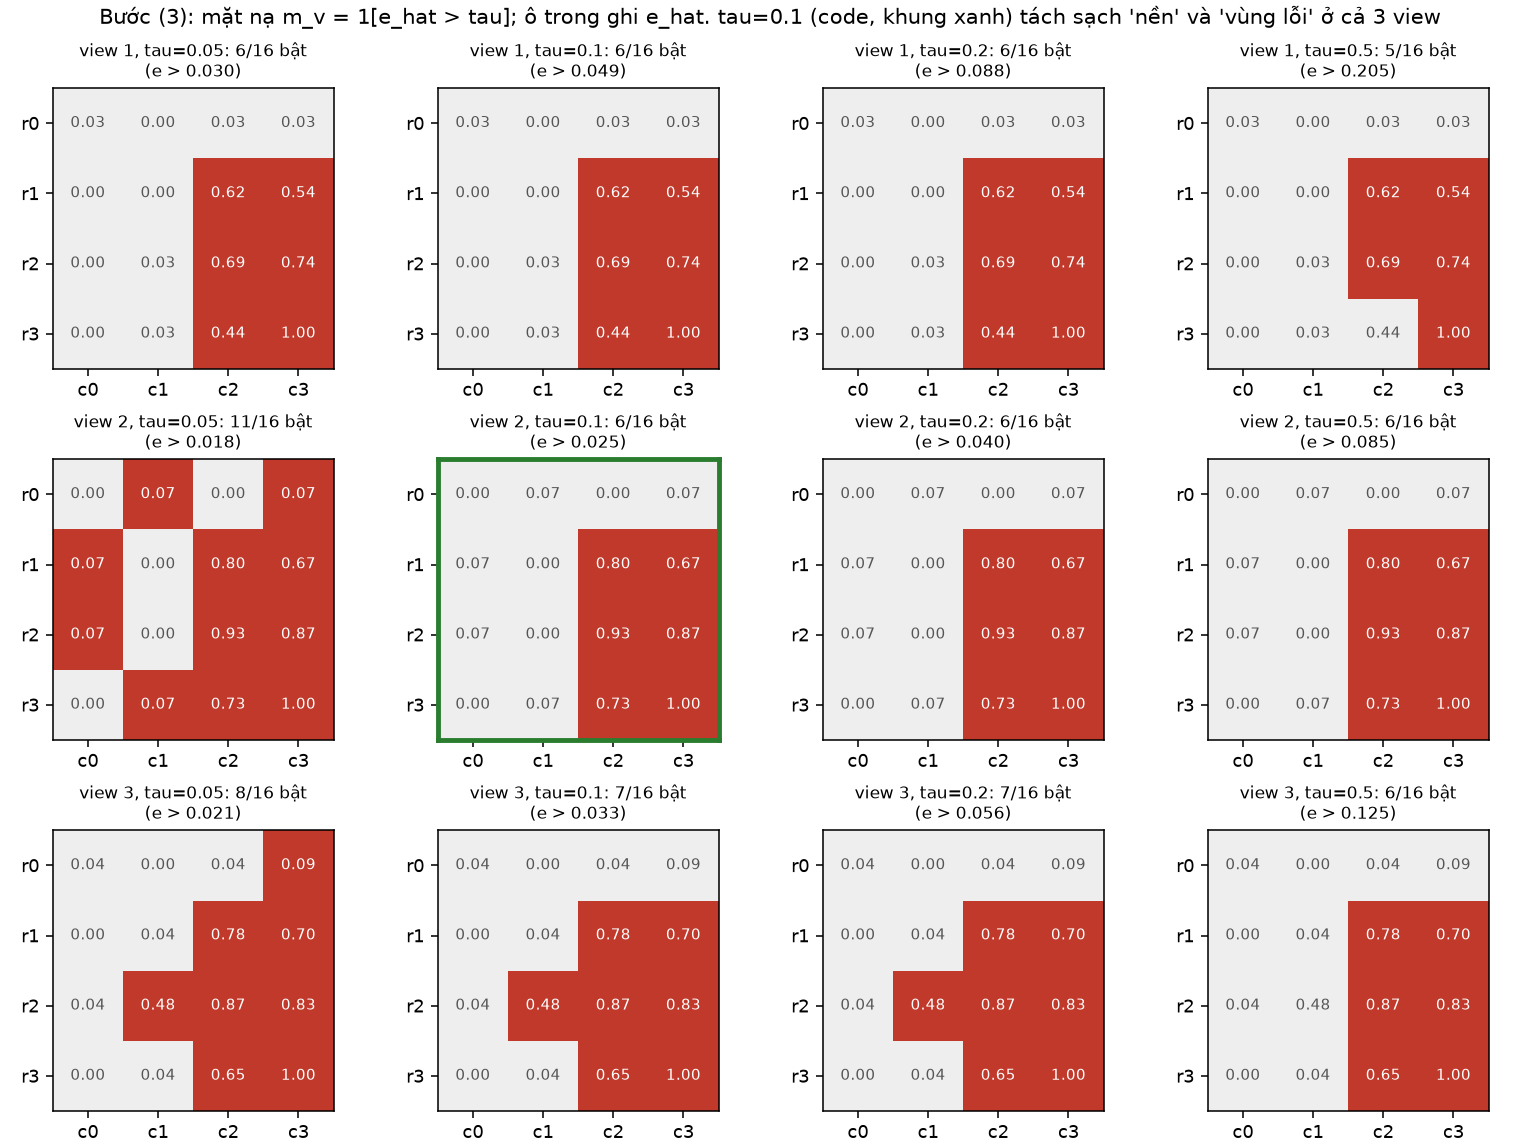
\includegraphics[width=0.95\linewidth]{1_8_tau_masks.png}
\captionof{figure}{\footnotesize Mặt nạ $m_v$ trên 3 view $\times$ 4 mức $\tau$; khung xanh = $\tau_{\text{loss}}=0.1$.}
\end{column}
\end{columns}
\end{frame}

% --- 1_9_tau_curve.png ---
\begin{frame}{Đường cong \% pixel bị đánh dấu theo $\tau$}
\begin{columns}[T]
\begin{column}{0.5\linewidth}
\footnotesize
\begin{itemize}
\item Với ảnh $4\times4$ (3 view $E_1,E_2,E_3$): đường \% pixel đánh dấu theo $\tau$ có dạng \textbf{bậc thang} do chỉ có 16 pixel rời rạc.
\item $\tau_{\text{loss}} = 0.1$ nằm trên một \textbf{bậc phẳng rộng} — nghĩa là kết quả mặt nạ \textbf{ổn định}, không nhạy với sai số nhỏ khi chọn $\tau$.
\item Với ảnh mô phỏng $48\times32$ ở 3 mức chất lượng khác nhau (max $e \approx 0.40$, $0.16$, $0.05$): sau khi min-max chuẩn hoá theo từng ảnh, đường cong \% pixel gần như \textbf{trùng nhau}.
\item Ý nghĩa: chuẩn hoá theo ảnh (per-image min-max) làm cho $\tau_{\text{loss}}$ mang \textbf{ý nghĩa tương đối}, không phụ thuộc chất lượng tuyệt đối của ảnh render.
\end{itemize}
\end{column}
\begin{column}{0.5\linewidth}
\centering
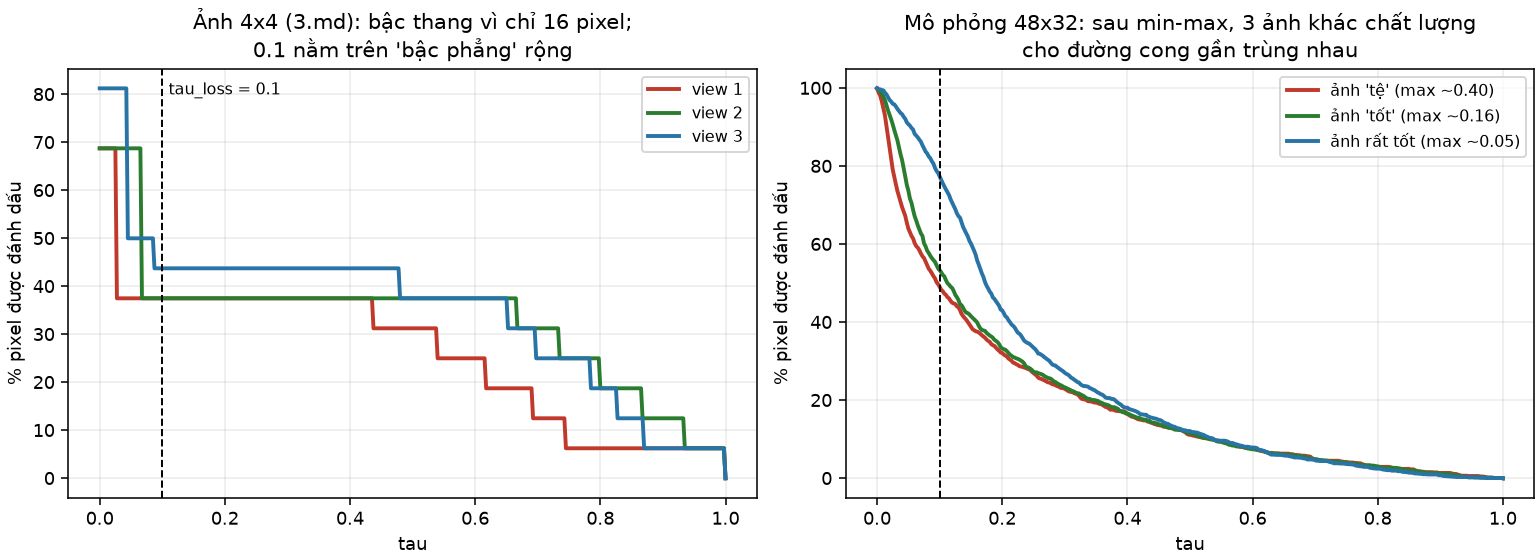
\includegraphics[width=0.98\linewidth]{1_9_tau_curve.png}
\captionof{figure}{\footnotesize Trái: \% pixel đánh dấu vs $\tau$ trên ảnh $4\times4$ (bậc thang, $\tau=0.1$ trên bậc phẳng). Phải: mô phỏng $48\times32$ ở 3 mức chất lượng, các đường gần trùng sau chuẩn hoá.}
\end{column}
\end{columns}
\end{frame}

% --- 1_10_equiv_threshold.png ---
\begin{frame}{Ngưỡng chuẩn hoá $\Leftrightarrow$ ngưỡng tuyệt đối trên $e$ gốc}
\begin{columns}[T]
\begin{column}{0.52\textwidth}
\scriptsize
\begin{itemize}
\item $\tau_{\text{loss}}{=}0.1$ trên $\tilde e$ tương đương ngưỡng tuyệt đối mỗi view: $e > e_{\min} + \tau_{\text{loss}}(e_{\max}-e_{\min})$.
\item Ví dụ 3 view: $[0.01,0.40],[0.01,0.16],[0.01,0.24]$ $\Rightarrow$ ngưỡng ${\approx}0.049,0.025,0.033$.
\item \textbf{Cùng $\tau_{\text{loss}}$} nhưng ngưỡng tuyệt đối mỗi view khác nhau: view càng "tệ" (khoảng rộng) ngưỡng càng cao.
\item Hệ quả của chuẩn hoá \textbf{theo từng ảnh} trước khi so với $\tau_{\text{loss}}$ cố định.
\end{itemize}
\end{column}
\begin{column}{0.48\textwidth}
\centering
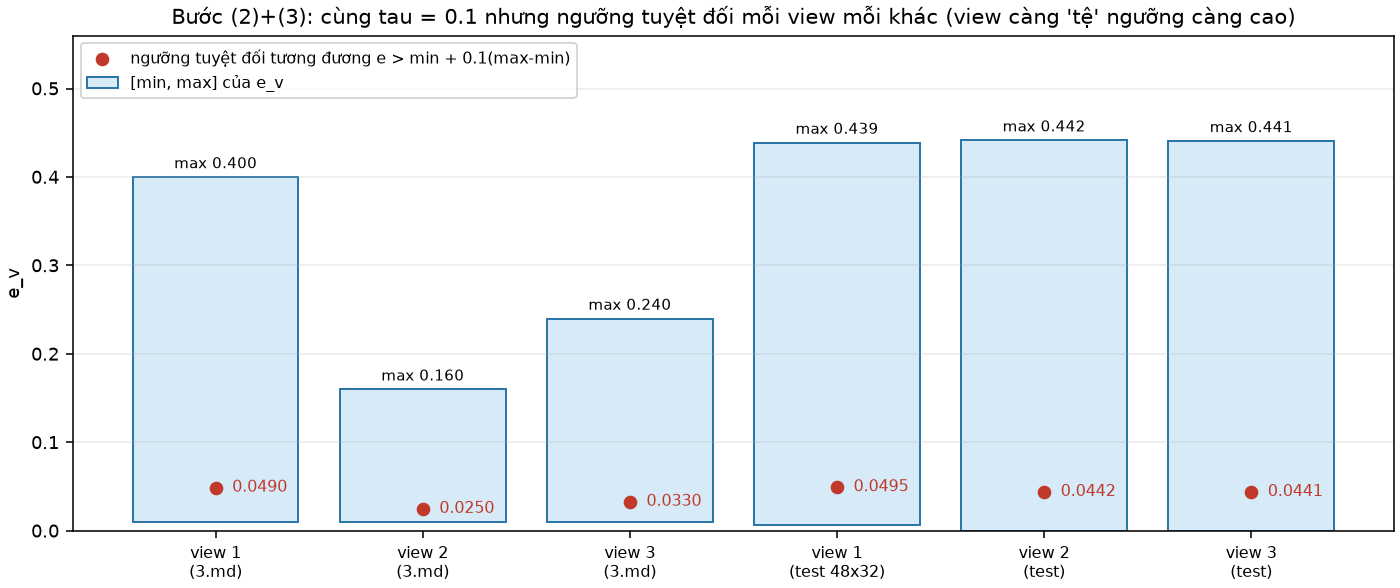
\includegraphics[width=0.95\linewidth]{1_10_equiv_threshold.png}
\captionof{figure}{\footnotesize Khoảng $[e_{\min},e_{\max}]$ mỗi view và ngưỡng tuyệt đối tương đương.}
\end{column}
\end{columns}
\end{frame}

% --- 1_11_edge_cases.png ---
\begin{frame}{Trường hợp biên: ảnh hoàn hảo, ảnh rất tệ, và chia cho 0}
\begin{columns}[T]
\begin{column}{0.5\linewidth}
\footnotesize
\begin{itemize}
\item \textbf{Ảnh hằng số} ($e_v \equiv 0.03$, mọi pixel bằng nhau): $e_{\max}-e_{\min}=0 \Rightarrow \tilde e = 0/0 = \text{NaN}$.
\item So sánh \texttt{NaN > 0.1} luôn trả về \texttt{False} trong PyTorch/NumPy $\Rightarrow$ mặt nạ \textbf{rỗng} (0/16 pixel) một cách \textbf{an toàn}, không crash, không cần epsilon.
\item \textbf{Ảnh gần hội tụ} ($e \in [0.004, 0.006]$, mẫu số rất nhỏ): min-max vẫn kéo giá trị về $[0,1]$ đầy đủ $\Rightarrow$ \textbf{nhiễu nhỏ bị phóng đại} thành "lỗi cao" — đây là cái giá của chuẩn hoá theo ảnh.
\item Nếu cộng thêm $\epsilon$ vào mẫu số (code \textbf{không} làm vậy): với $\epsilon < 10^{-3}$, ảnh hưởng lên $\tilde e$ dưới $1\%$ — không đáng kể trong thực tế.
\end{itemize}
\end{column}
\begin{column}{0.5\linewidth}
\centering
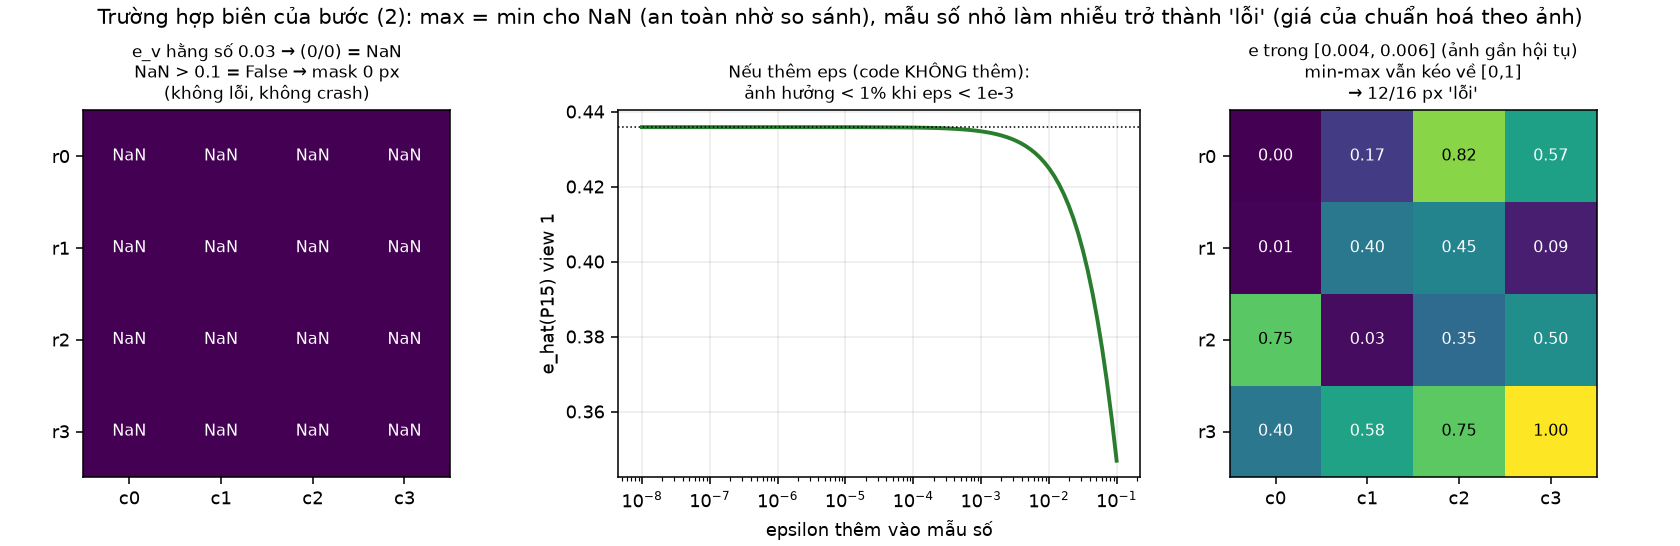
\includegraphics[width=0.98\linewidth]{1_11_edge_cases.png}
\captionof{figure}{\footnotesize (a) $e$ hằng số $\to$ NaN, mặt nạ rỗng an toàn. (b) Ảnh hưởng của $\epsilon$ giả định lên $\tilde e$. (c) $e$ nhỏ (ảnh gần hội tụ) vẫn bị min-max kéo về $[0,1]$.}
\end{column}
\end{columns}
\end{frame}

% --- 1_12_torch_flow.png ---
\begin{frame}{Luồng PyTorch thực tế: từ render đến mặt nạ (\texttt{get\_loss})}
\scriptsize
\begin{itemize}
\item \textbf{B1 — L1}: \texttt{torch.abs(rend-gt)} $[3,H,W]$ $\to$ \texttt{mean(.,0)} $\to$ \texttt{l1\_loss} $[H,W]$.
\item \textbf{B2 — minmax}: $\frac{\text{l1\_loss}-\min}{\max-\min} \to$ \texttt{l1\_loss\_norm}$\in[0,1]$, min/max trên \textbf{toàn ảnh}.
\item \textbf{B3 — ngưỡng}: \texttt{(l1\_loss\_norm>0.1).int()} $\to$ \texttt{metric\_map}$\in\{0,1\}$. Hàm: \texttt{get\_loss()} (\texttt{utils/fast\_utils.py:21-25}).
\item \texttt{metric\_map} truyền vào \texttt{render\_fastgs(...,metric\_map=...)} — \textbf{bước 4}, cầu nối sang importance đa view (Phần 2).
\end{itemize}
\centering
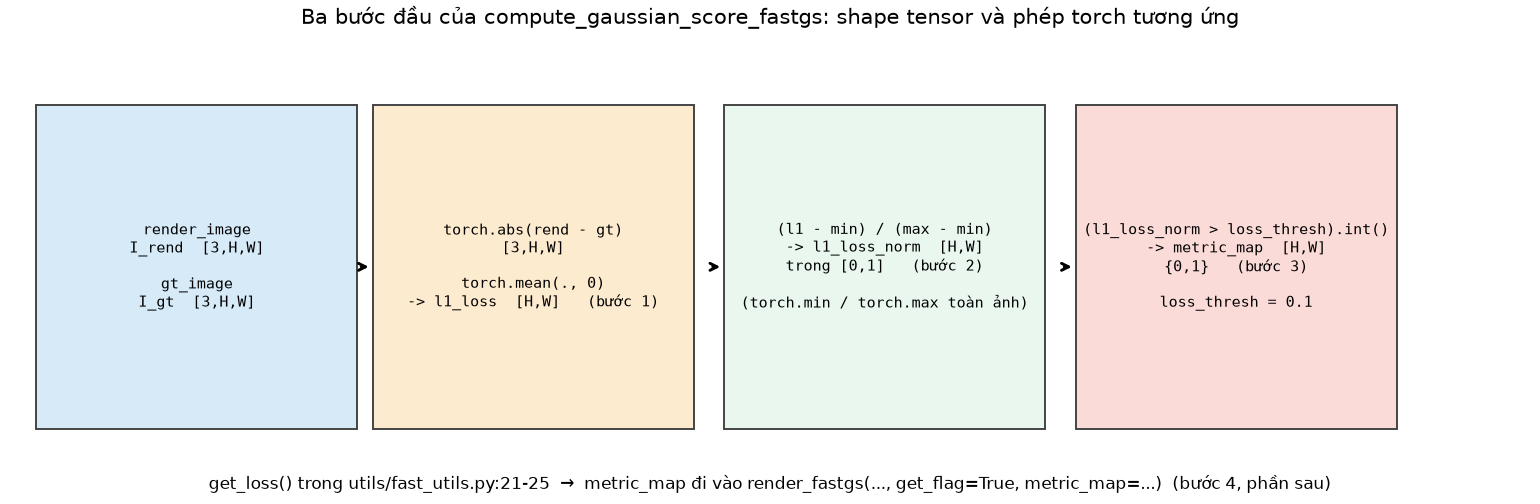
\includegraphics[width=0.68\linewidth]{1_12_torch_flow.png}
\captionof{figure}{\footnotesize Tensor shape qua 3 bước: render/gt $\to$ l1\_loss $\to$ l1\_loss\_norm $\to$ metric\_map.}
\end{frame}


\section{ADC chuyên sâu — P2: Footprint \& Importance đa view}
% partADC_2a.tex — Adaptive Density Control, Phần 2a: Footprint & Importance (bước 4-5)
% 6 frame, dùng lại figures/ đã có trong main.tex (graphicspath)

% --- 2_1_footprint-mot-gaussian.png ---
\begin{frame}{Footprint thật của một Gaussian không phải là ellipse hình học}
    \begin{columns}[T]
        \begin{column}{0.46\textwidth}
            \footnotesize
            \begin{itemize}
                \item Với mỗi pixel $p$, khoảng cách Mahalanobis:
                \[
                    d_M^2(p) = (p-\mu)^\top \Sigma'^{-1} (p-\mu)
                \]
                và độ mờ (opacity hiệu dụng):
                \[
                    \alpha(p) = \min\!\big(0.99,\ o \cdot e^{-\tfrac{1}{2} d_M^2(p)}\big)
                \]
                \item (a) Ellipse hình học 3$\sigma$: $d_M^2 \le 9$ — chỉ là hình dạng lý thuyết.
                \item (b) Sau cull compact-box (mult $=0.5$): $d_M^2 \le t_{cb} = \ln(255\,o)$.
                \item (c) Chỉ giữ pixel có $\alpha(p) \ge 1/255$ (ngưỡng hiển thị).
                \item (d) Footprint \textbf{hữu hình} $\Omega_i^v$: giao (b) $\cap$ (c) $\cap$ \{pixel chưa bị che, $T \ge 10^{-4}$\}.
            \end{itemize}
        \end{column}
        \begin{column}{0.5\textwidth}
            \centering
            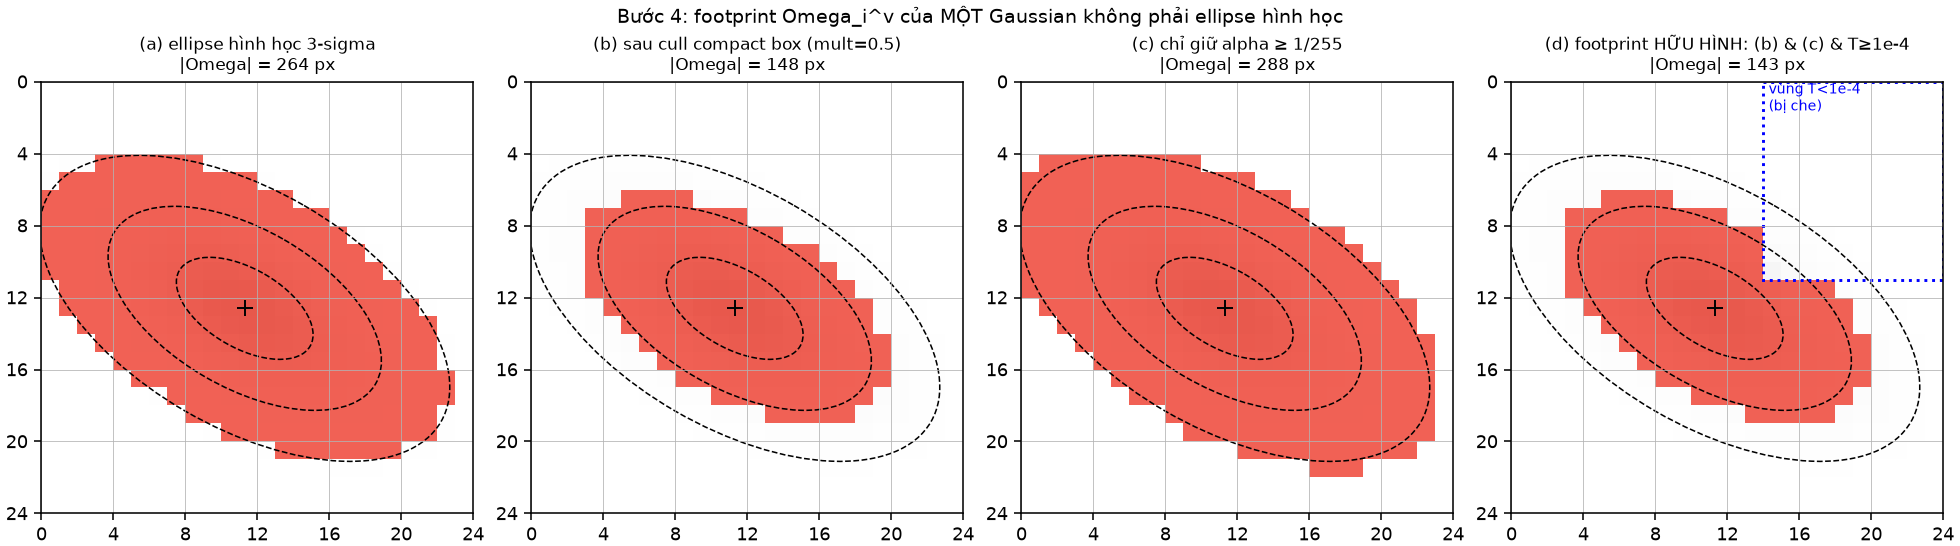
\includegraphics[width=0.98\linewidth]{2_1_footprint-mot-gaussian.png}
            \captionof{figure}{\footnotesize 4 định nghĩa footprint khác nhau cho cùng một Gaussian: chỉ (d) mới là $\Omega_i^v$ dùng để đếm lỗi.}
        \end{column}
    \end{columns}
\end{frame}

% --- 2_2_nhieu-gaussian-chong-nhau.png ---
\begin{frame}{Nhiều Gaussian chồng lấn: một pixel lỗi ``tố cáo'' tất cả}
    \footnotesize
    \begin{itemize}
        \item Ba Gaussian $A$ (gần, $\alpha=0.95$), $B$ (giữa, $\alpha=0.5$), $C$ (xa, $\alpha=0.7$) có footprint chồng lên nhau.
        \item Độ trong suốt tích lũy cập nhật theo thứ tự alpha-blending (gần $\to$ xa):
        \[
            T \leftarrow T \cdot (1 - \alpha(p)) \quad \text{nếu } p \in \Omega \text{ và } \alpha(p) \ge 1/255
        \]
        \item Điều kiện Gaussian còn "sống" tại pixel đó (early-out): $T \ge 10^{-4}$ — nếu $T < 10^{-4}$, các Gaussian ở sau bị loại khỏi $\Omega$.
        \item Vì vậy \textbf{không thể} chỉ nhìn màu pixel cuối cùng để suy ra Gaussian nào gây lỗi — phải đếm/tổng hợp riêng đóng góp của từng Gaussian có mặt trong $\Omega_i^v$.
        \item Một pixel có thể thuộc 0, 1, 2 hoặc cả 3 footprint cùng lúc.
    \end{itemize}
    \centering
    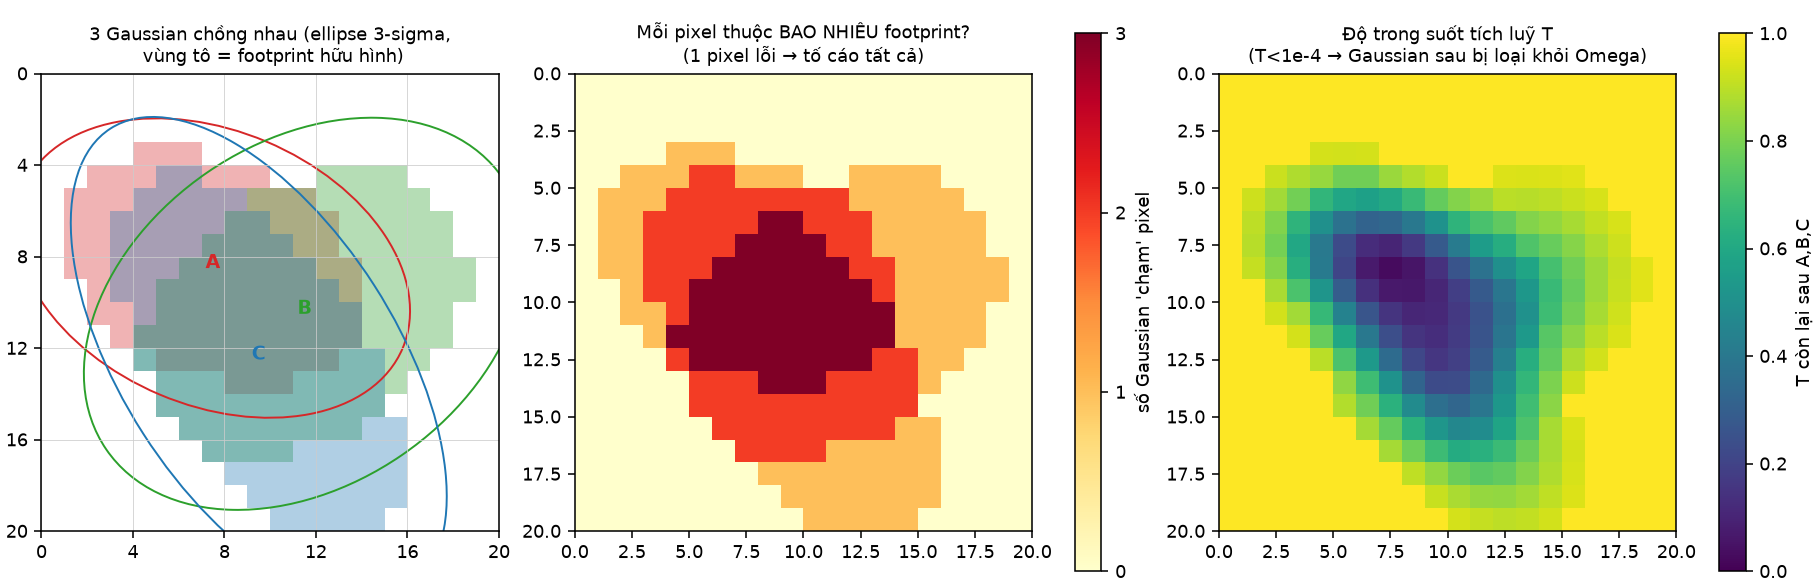
\includegraphics[width=0.75\linewidth]{2_2_nhieu-gaussian-chong-nhau.png}
    \captionof{figure}{\footnotesize Trái: 3 footprint chồng nhau. Giữa: số Gaussian "chạm" mỗi pixel. Phải: $T$ còn lại sau $A,B,C$.}
\end{frame}

% --- 2_3_giao-mat-na-footprint.png ---
\begin{frame}{Giao mặt nạ lỗi $m_v$ với footprint $\Omega_i^v$: chỉ phần giao mới được tính}
    \footnotesize
    \begin{itemize}
        \item Ví dụ minh họa: lưới $4\times 4$ (16 pixel), 5 Gaussian $G1$--$G5$, 3 view.
        \item Mặt nạ lỗi cao mỗi view: $|m_1| = |m_2| = 6$ pixel, $|m_3| = 7$ pixel.
        \item Với mỗi Gaussian $i$ và view $v$:
        \[
            \text{counts}_i^v = \big|\, \Omega_i^v \cap m_v \,\big|
        \]
        \item Ví dụ $G4$: $|\Omega_4^1|=6, |\Omega_4^2|=4, |\Omega_4^3|=3$ — kích thước footprint co lại qua các view do bị che khuất một phần.
        \item $G5$ chỉ hữu hình ở view 1 ($\Omega_5^2=\Omega_5^3=\varnothing$) — Gaussian bị che hoàn toàn ở view 2, 3 không đóng góp gì.
    \end{itemize}
    \centering
    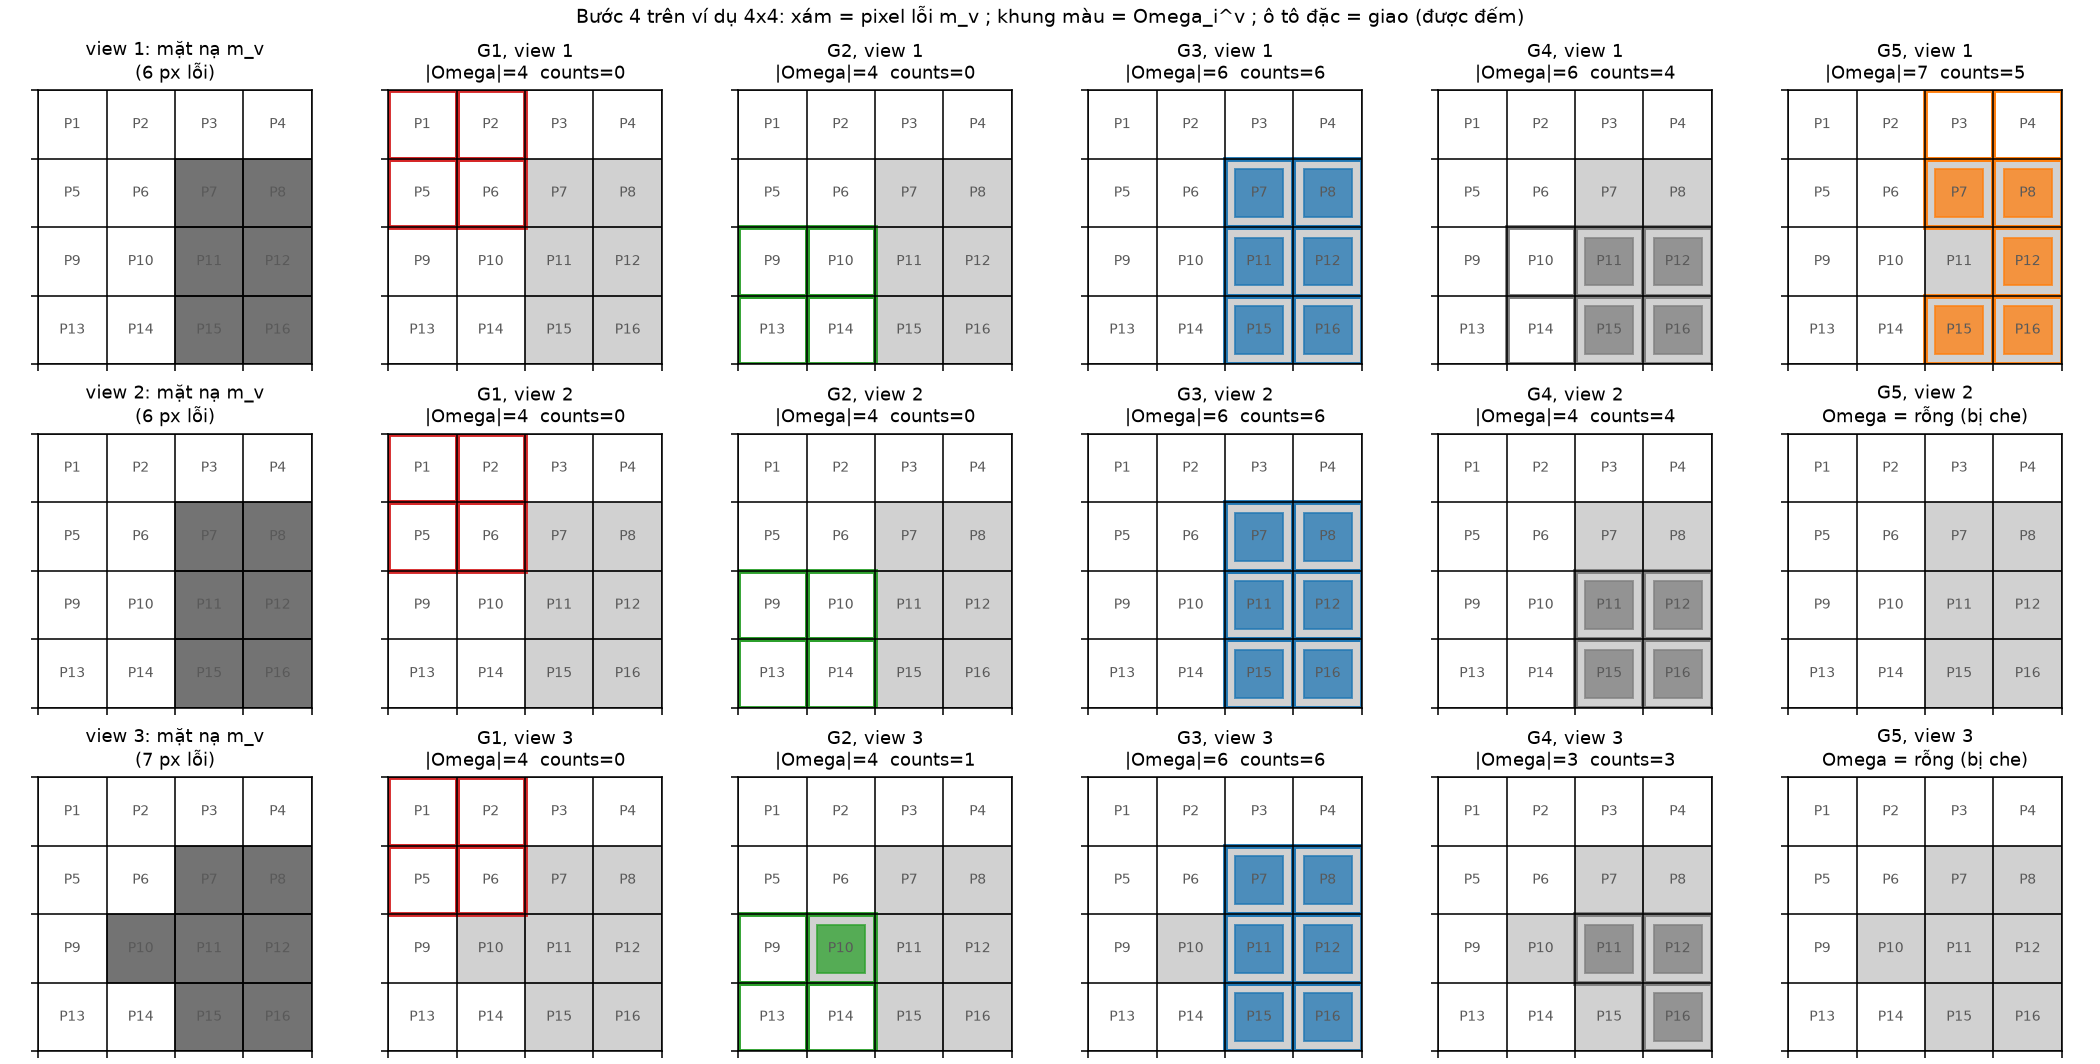
\includegraphics[width=0.62\linewidth]{2_3_giao-mat-na-footprint.png}
    \captionof{figure}{\footnotesize Xám = pixel lỗi $m_v$; khung màu = $\Omega_i^v$; ô tô đặc = phần giao (được đếm vào counts).}
\end{frame}

% --- 2_4_bar-counts-moi-view.png ---
\begin{frame}{Tổng hợp counts qua nhiều view: đầu vào cho Importance}
    \footnotesize
    \begin{itemize}
        \item Với ví dụ $4\times4$ ở trên: mỗi Gaussian $i$ có một vector counts $(\text{counts}_i^1, \text{counts}_i^2, \text{counts}_i^3)$, nền xám là kích thước footprint $|\Omega_i^v|$ tương ứng.
        \item Tổng số lỗi bị "tố cáo" trên mỗi view luôn $\ge$ số pixel lỗi thật:
        \[
            \sum_i \text{counts}_i^v \ \ge\ |m_v|
        \]
        vì một pixel lỗi có thể được nhiều Gaussian chồng lấn cùng đếm.
        \item Trong code: mỗi lần render một view $v$, kernel CUDA cộng dồn atomic vào tensor \texttt{metricCount}$[N]$, rồi cộng lũy kế: \texttt{full\_metric\_counts += counts\textsuperscript{(v)}}.
        \item Vector counts theo Gaussian, tổng hợp qua $V$ view, là đầu vào trực tiếp cho bước tính Importance.
    \end{itemize}
    \centering
    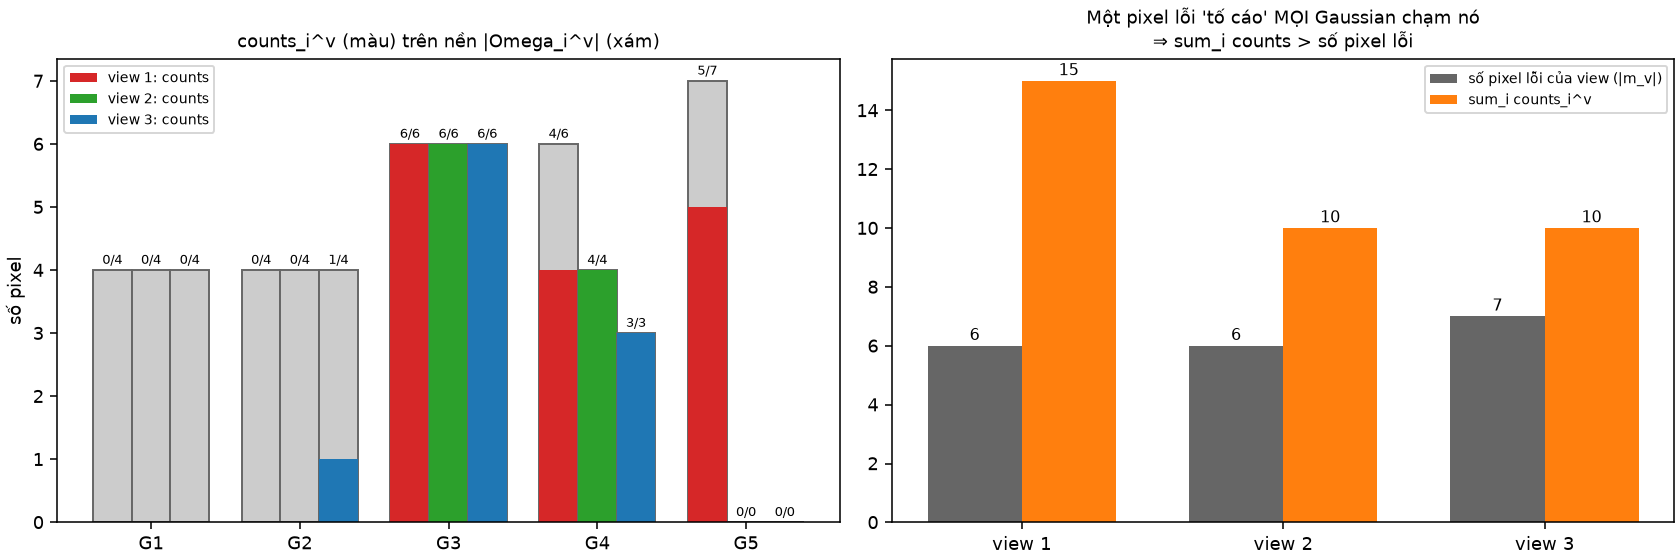
\includegraphics[width=0.85\linewidth]{2_4_bar-counts-moi-view.png}
    \captionof{figure}{\footnotesize Trái: counts$_i^v$ (màu) trên nền $|\Omega_i^v|$ (xám) từng Gaussian. Phải: tổng $|m_v|$ so với $\sum_i \text{counts}_i^v$ mỗi view.}
\end{frame}

% --- 2_5_importance-heatmap.png ---
\begin{frame}{Importance score: trung bình counts qua các view, làm tròn xuống}
    \footnotesize
    \begin{itemize}
        \item Công thức Importance (khớp code \texttt{compute\_gaussian\_score\_fastgs}):
        \[
            \text{Importance}_i = \left\lfloor \frac{1}{V} \sum_{v=1}^{V} \text{counts}_i^v \right\rfloor
        \]
        (\texttt{torch.div(full\_metric\_counts, V, rounding\_mode='floor')}).
        \item Gaussian được xem là "quan trọng" (giữ lại/densify) khi $\text{Importance}_i > 5$.
        \item Trong ví dụ $4\times4$, $3$ view: chỉ $G3$ có mean $> 5$ và vượt ngưỡng; các Gaussian còn lại (kể cả $G5$ với mean $=1.67$) bị chặn.
        \item Nếu thay trung bình bằng $\max_v$ hay $\sum_v$: $G5$ có $\max=5, \sum=5$ — vẫn không vượt ngưỡng $>5$, nhưng thứ hạng tương đối giữa các Gaussian có thể đổi khác so với dùng mean.
        \item Màu nóng trong heatmap = Gaussian đóng góp nhiều vào vùng lỗi cao (giữ lại); màu lạnh = ứng viên prune.
    \end{itemize}
    \centering
    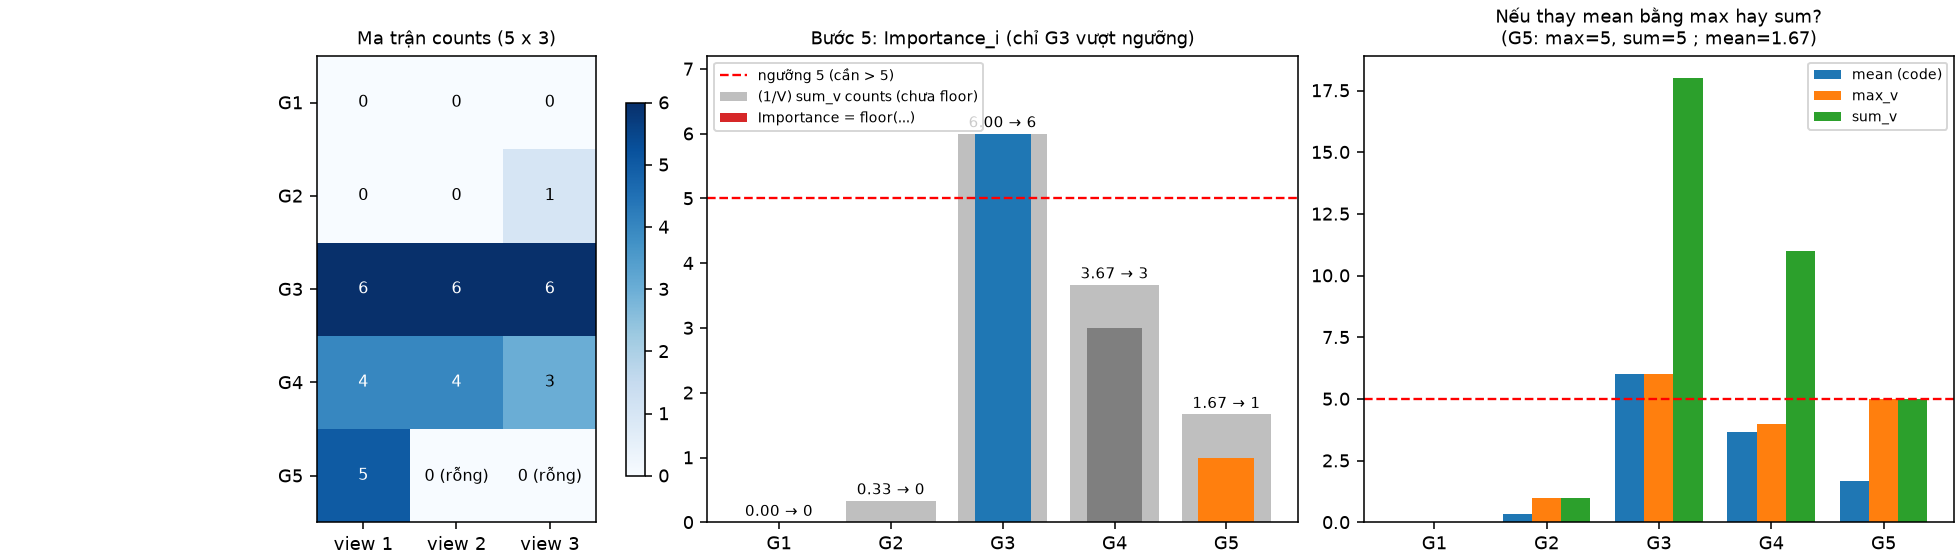
\includegraphics[width=0.85\linewidth]{2_5_importance-heatmap.png}
    \captionof{figure}{\footnotesize Trái: ma trận counts $(5\times 3)$. Giữa: Importance$_i = \lfloor \text{mean}_v \rfloor$, ngưỡng $5$. Phải: so sánh mean vs.\ max vs.\ sum.}
\end{frame}

% --- 2_6_mo-phong-200-gaussian.png ---
\begin{frame}{Kiểm chứng ở quy mô lớn: mô phỏng 200 Gaussian, $V=10$ view}
    \footnotesize
    \begin{itemize}
        \item Mô hình mô phỏng: kích thước footprint $|\Omega_i| \sim \exp\big(U(\ln 4, \ln 3000)\big)$, tỉ lệ lỗi trong footprint $\rho_i \sim \text{Beta}(0.7, 4.0)$, xác suất hữu hình mỗi view $p_{vis} \sim U(0.3, 1.0)$.
        \item Với mỗi view: hữu hình với xác suất $p_{vis}$, khi đó $\text{counts}_i^v \sim \text{Binomial}(|\Omega_i|, \rho_i)$; nếu không hữu hình thì counts $=0$.
        \item Importance$_i = \left\lfloor \frac{1}{V}\sum_v \text{counts}_i^v \right\rfloor$ như công thức đã dùng ở slide trước.
        \item Phân bố Importance không tập trung/lệch bất thường: một số vượt ngưỡng $5$, một số bằng $0$ — phù hợp trực giác Importance $\approx |\Omega_i| \cdot \rho_i \cdot p_{vis}$ (Gaussian to, tỉ lệ lỗi cao, hữu hình nhiều view dễ vượt ngưỡng hơn).
        \item Gaussian nhỏ dù có tỉ lệ lỗi cao (counts/$|\Omega|$ lớn) vẫn dễ bị chặn vì số pixel tuyệt đối thấp.
    \end{itemize}
    \centering
    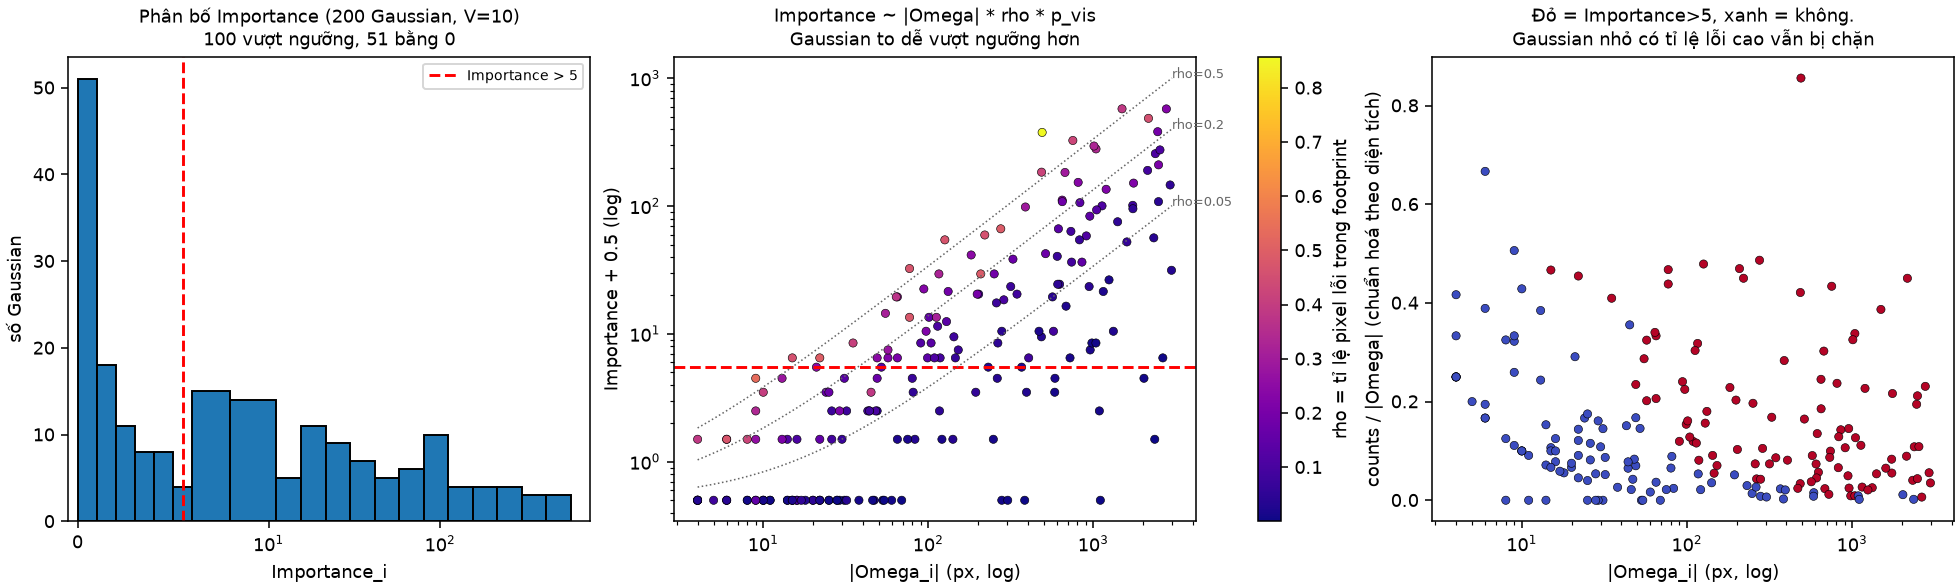
\includegraphics[width=0.85\linewidth]{2_6_mo-phong-200-gaussian.png}
    \captionof{figure}{\footnotesize Trái: phân bố Importance trên 200 Gaussian. Giữa: Importance theo $|\Omega|$, màu theo $\rho$. Phải: đỏ = Importance$>5$, xanh = không.}
\end{frame}

% partADC_2b.tex --- Phan ADC-2b: Adaptive Density Control (chuyen sau)
% Khong co \documentclass / \usepackage / \begin{document} -- duoc \input tu main.tex

% --- 2_7_monte-carlo-V.png ---
\begin{frame}{Ước lượng Monte Carlo cho Importance khi $V$ nhỏ}
\begin{columns}[T]
\begin{column}{0.5\linewidth}
\footnotesize
\begin{itemize}
  \item Trong huấn luyện thật, ta chỉ lấy mẫu $V \ll V_{\text{all}}$ view (VD $V=1,3,10,30$) thay vì duyệt hết $V_{\text{all}}=200$ view.
  \item Với mỗi $V$, chọn ngẫu nhiên $V$ view (không lặp) trong $3000$ lần thử, tính
  $$\widehat{\text{Imp}}_i = \left\lfloor \frac{1}{V}\sum_{v\in\text{mẫu}} \text{counts}_i^{(v)} \right\rfloor$$
  \item Ba loại Gaussian mô phỏng: (A) lỗi nhất quán ($p_{\text{vis}}=0.9$, Poisson$(8)$), (B) artefact 1 góc ($p_{\text{vis}}=0.05$, Poisson$(60)$), (C) biên giới ($p_{\text{vis}}=0.6$, Poisson$(9)$).
  \item Khi $V\!\uparrow$: trung bình ước lượng hội tụ về giá trị "toàn bộ" (đường chấm, $V{=}200$); độ lệch chuẩn giảm xấp xỉ $\propto 1/V$.
  \item Loại B (artefact hiếm gặp) có phương sai ước lượng lớn nhất — dễ bị bỏ sót hoặc đánh giá sai khi $V$ nhỏ.
\end{itemize}
\end{column}
\begin{column}{0.5\linewidth}
\centering
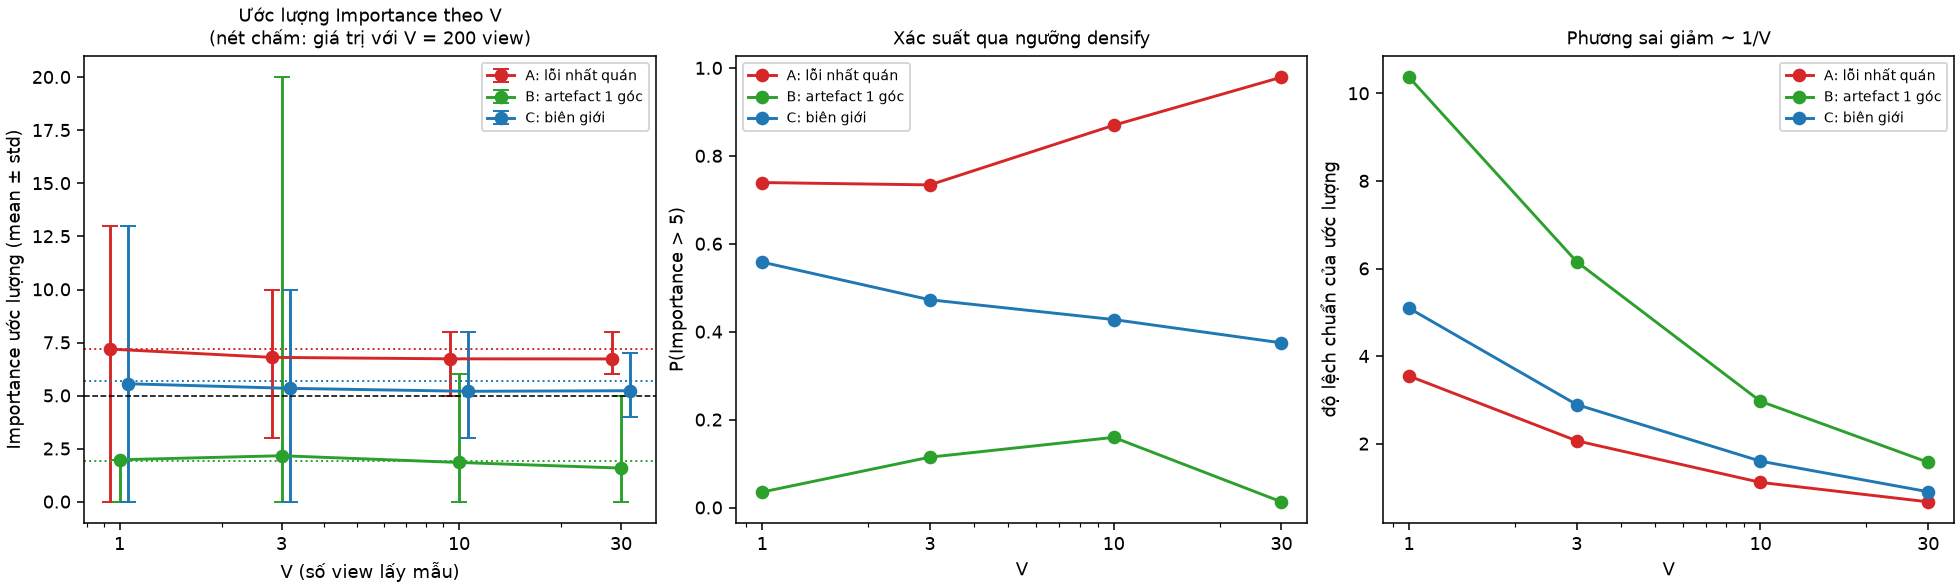
\includegraphics[width=0.95\linewidth]{2_7_monte-carlo-V.png}
\captionof{figure}{\footnotesize Importance ước lượng (mean $\pm$ std) và $P(\text{Importance}>5)$ theo số view lấy mẫu $V$.}
\end{column}
\end{columns}
\end{frame}

% --- 2_8_3dgs-vs-fastgs.png ---
\begin{frame}{3DGS gốc và FastGS-lite: hai tín hiệu densify khác nhau}
\begin{columns}[T]
\begin{column}{0.5\linewidth}
\footnotesize
\begin{itemize}
  \item \textbf{3DGS gốc}: chỉ dùng gradient tích luỹ trung bình $\|g_i\| \ge \tau$, với $\tau = 2\times 10^{-4}$ (ngưỡng densify chuẩn).
  \item \textbf{FastGS-lite}: thêm điều kiện \emph{AND} với Importance đa view giao mặt nạ lỗi:
  $$\|g_i\| \ge \tau \;\land\; \text{Importance}_i > 5$$
  \item Trên quần thể mô phỏng $n=400$ Gaussian ($V=10$ view): 3DGS densify toàn bộ Gaussian có gradient vượt ngưỡng, kể cả khi Importance thấp (điểm đỏ, dấu $\times$).
  \item FastGS-lite loại bỏ đúng những Gaussian có gradient cao nhưng \emph{không} liên quan đến lỗi ảnh hiện tại (Importance $\le 5$) — giảm số ứng viên densify mỗi vòng.
  \item Kết quả: số Gaussian được densify giảm mạnh so với 3DGS gốc trong cùng quần thể — tác động luỹ thừa lên tốc độ tăng $N$ qua nhiều vòng lặp.
\end{itemize}
\end{column}
\begin{column}{0.5\linewidth}
\centering
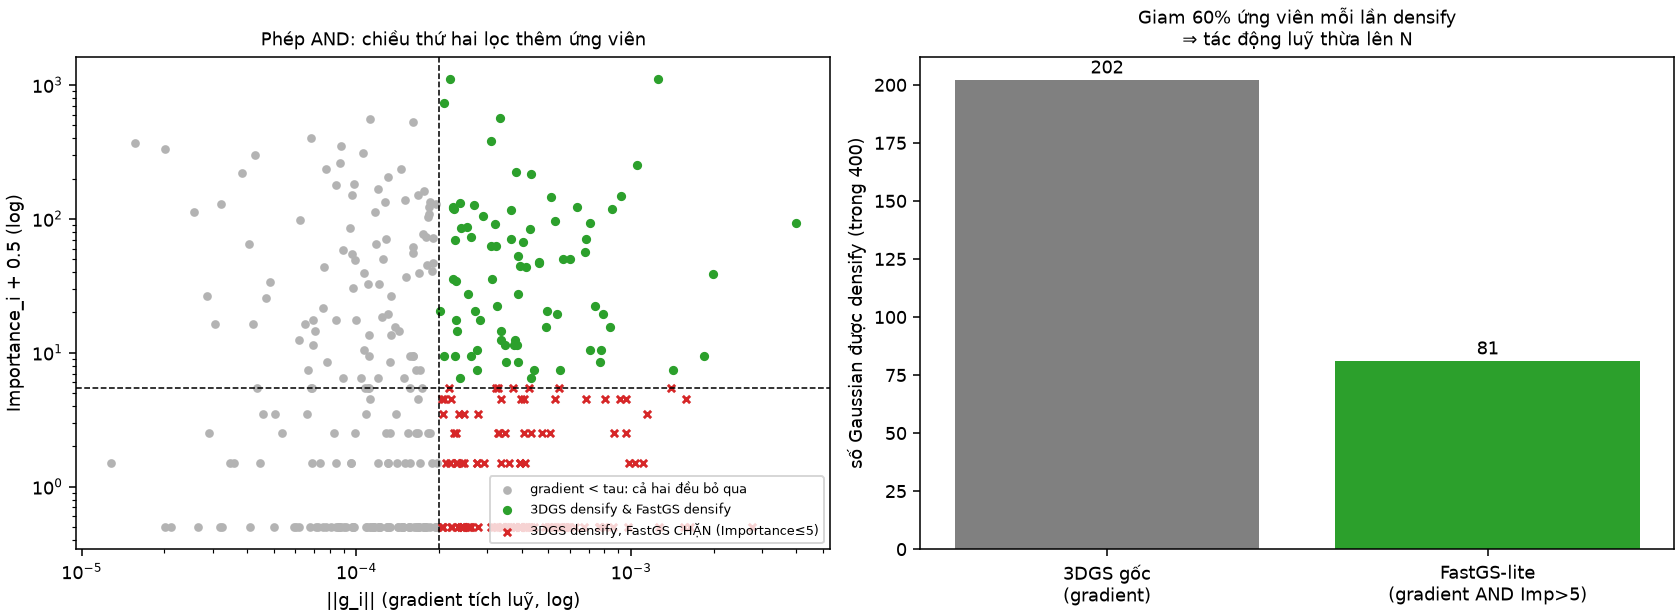
\includegraphics[width=0.95\linewidth]{2_8_3dgs-vs-fastgs.png}
\captionof{figure}{\footnotesize Trái: phép AND lọc thêm theo Importance. Phải: số Gaussian được densify, 3DGS gốc so với FastGS-lite.}
\end{column}
\end{columns}
\end{frame}

% --- 2_9_so-do-tensor.png ---
\begin{frame}{Sơ đồ tensor: luồng dữ liệu bước 4--5}
\footnotesize
Nguồn: \texttt{utils/fast\_utils.py: compute\_gaussian\_score\_fastgs} và \texttt{forward.cu:406-408}.
\begin{itemize}
  \item \texttt{render\_fastgs(cam\_v)} $\to$ ảnh render \texttt{[3,H,W]}.
  \item \texttt{get\_loss}: $e_v = \text{mean}_{ch}|r-g|$ \texttt{[H,W]}, minmax-chuẩn hoá $\to \hat e_v$ \texttt{[H,W]}.
  \item \texttt{metric\_map} $= (\hat e_v > 0.1)$.int() \texttt{[H,W]} $\in \{0,1\}$ -- mặt nạ pixel lỗi.
  \item Kernel CUDA duyệt từng (pixel, Gaussian): điều kiện \texttt{power<=0}, \texttt{alpha>=1/255}, \texttt{T>=1e-4}; nếu \texttt{metric\_map[pix]==1} thì \texttt{atomicAdd(metricCount[id], 1)} $\to$ \texttt{metricCount} \texttt{[N]} int32.
  \item Cộng dồn qua $V=\texttt{len(camlist)}=10$ view: \texttt{full\_metric\_counts += counts\textasciicircum(v)} \texttt{[N]} int.
  \item \texttt{importance\_score = torch.div(full\_metric\_counts, V, rounding\_mode='floor')} \texttt{[N]} int.
  \item (Phần sau) \texttt{full\_metric\_score += E\_photo\textasciicircum(v)} $\cdot$ \texttt{counts\textasciicircum(v)} $\to$ \texttt{pruning\_score} = minmax$_N(\cdot)$ \texttt{[N]} float -- dùng ở bước 6--7.
\end{itemize}
\centering
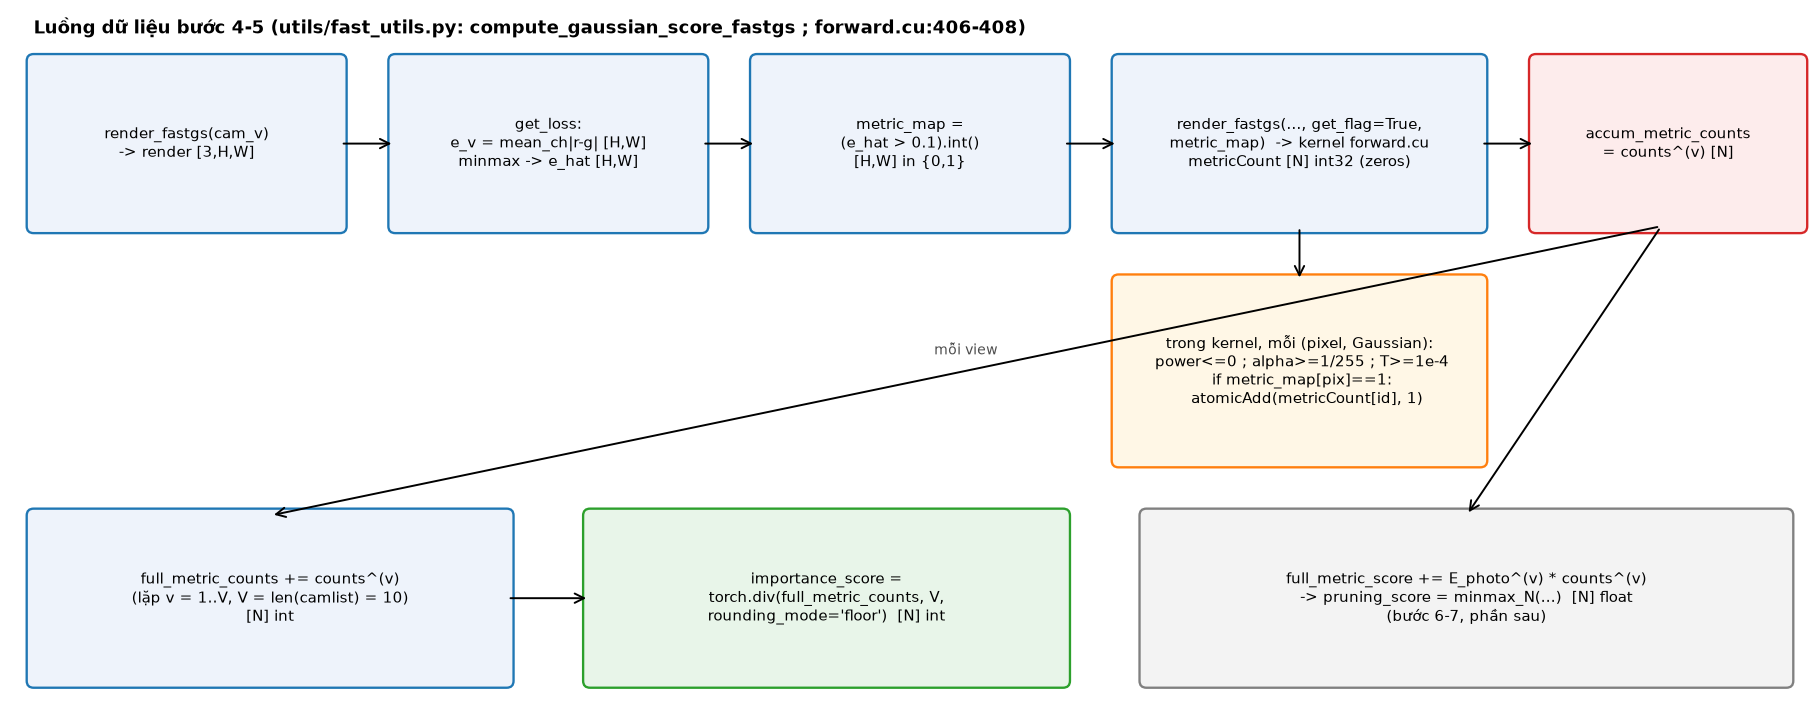
\includegraphics[width=0.75\linewidth]{2_9_so-do-tensor.png}
\captionof{figure}{\footnotesize Shape tensor qua từng phép toán: $N$ Gaussian $\times$ $H{\times}W$ pixel $\times$ $V$ view.}
\end{frame}

% --- 2_10_floor-va-nguong.png ---
\begin{frame}{Hiệu ứng \texttt{floor()} và ngưỡng chặt "$>5$"}
\begin{columns}[T]
\begin{column}{0.5\linewidth}
\footnotesize
\begin{itemize}
  \item Với $V=10$: $\text{Importance}_i = \left\lfloor \dfrac{\sum_v \text{counts}_i^{(v)}}{V} \right\rfloor$, so sánh chặt \emph{lớn hơn} $5$.
  \item Do làm tròn xuống, cần $\sum_v \text{counts}_i^{(v)} \ge 60$ ($=6V$) mới vượt ngưỡng — trung bình \emph{ít nhất} $6$ pixel lỗi/view.
  \item Vùng "nguy hiểm": tổng trong $[50,60)$ $\Rightarrow$ trung bình $\in [5,6)$ $\Rightarrow$ \texttt{floor}$=5$ $\Rightarrow$ \textbf{không} qua ngưỡng, dù rất gần.
  \item Nếu Gaussian chỉ hữu hình ở $k$ trong $10$ view và bị tô $c$ pixel lỗi mỗi lần hữu hình, cần $c \ge 60/k$ — Gaussian hữu hình ở ít view bị "dìm" xuống dù lỗi cục bộ nặng.
  \item Đây là cơ chế ép tính \emph{nhất quán đa góc nhìn}: lỗi thoáng qua ở 1--2 view không đủ kích hoạt densify.
\end{itemize}
\end{column}
\begin{column}{0.5\linewidth}
\centering
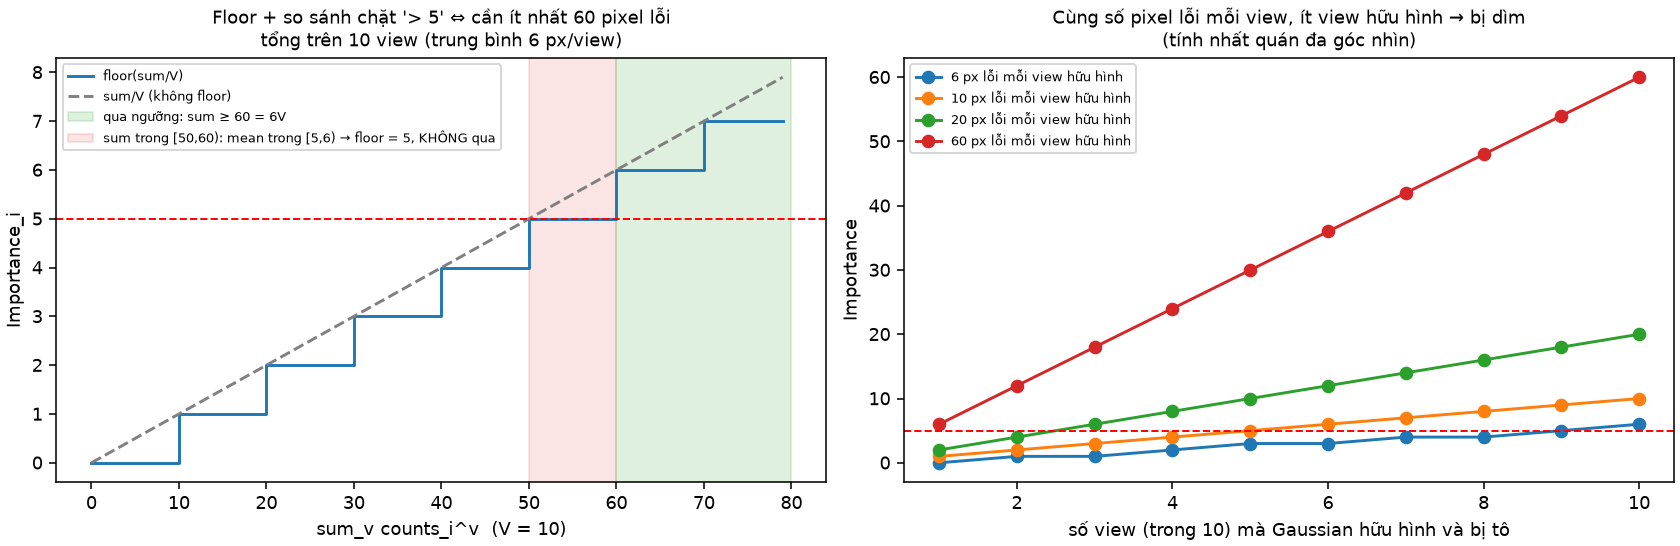
\includegraphics[width=0.95\linewidth]{2_10_floor-va-nguong.png}
\captionof{figure}{\footnotesize Trái: floor(sum/V) so với sum/V liên tục. Phải: Importance theo số view hữu hình $k$, với các mức lỗi/view $c=6,10,20,60$.}
\end{column}
\end{columns}
\end{frame}

% --- 2_11_canh-do-choi-48x32.png ---
\begin{frame}{Ví dụ kiểm định số trên cảnh đồ chơi $48\times 32$}
\begin{columns}[T]
\begin{column}{0.5\linewidth}
\footnotesize
\begin{itemize}
  \item Ảnh $48\times 32 = 1536$ pixel, $3$ view, $4$ Gaussian (G1--G4); vì gần như toàn ảnh đều sai nên \texttt{counts} $\approx |\Omega|$.
  \item Số pixel lỗi mỗi view: $|m_v| = 1409,\ 1077,\ 1042$ (view 1,2,3).
  \item \texttt{counts}/$|\Omega|$ luôn $\ge 0.9$ — hầu hết footprint của mỗi Gaussian nằm trong vùng lỗi.
  \item Tổng \texttt{counts} qua $3$ view của mỗi Gaussian lớn hơn nhiều so với $|m_v|$ của một view đơn lẻ (một pixel lỗi "tố cáo" nhiều Gaussian cùng lúc).
  \item Importance kết quả cho G1--G4 lần lượt xấp xỉ $1044,\ 1017,\ 1066,\ 974$ — vượt xa ngưỡng $5$ vì cảnh đồ chơi cố tình làm sai toàn bộ khung hình.
\end{itemize}
\end{column}
\begin{column}{0.5\linewidth}
\centering
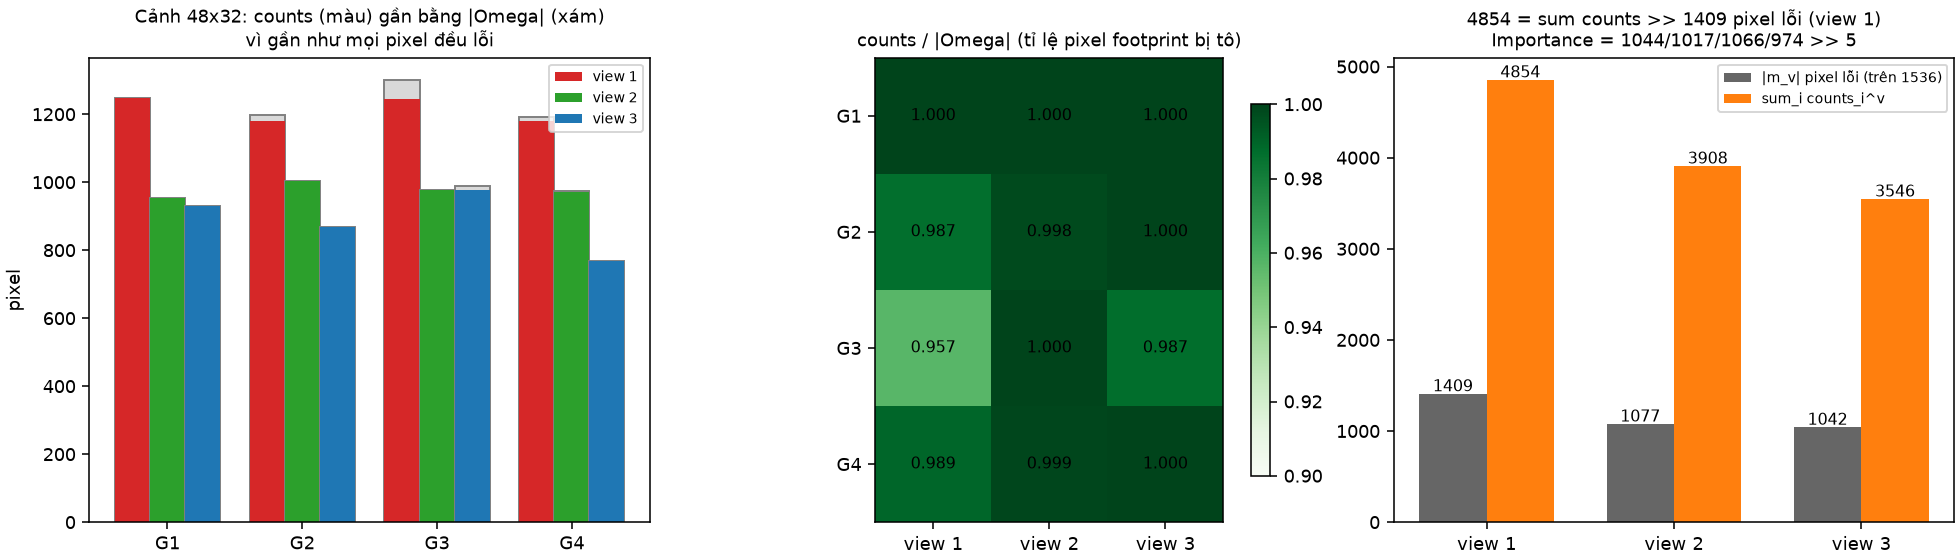
\includegraphics[width=0.95\linewidth]{2_11_canh-do-choi-48x32.png}
\captionof{figure}{\footnotesize Trái: counts (màu) trên nền $|\Omega|$ (xám). Giữa: tỉ lệ counts/$|\Omega|$. Phải: tổng counts so với $|m_v|$.}
\end{column}
\end{columns}
\end{frame}

% --- 2_12_to-vs-nho.png ---
\begin{frame}{Gaussian TO và NHỎ: cùng mặt nạ lỗi, Importance khác nhau}
\begin{columns}[T]
\begin{column}{0.5\linewidth}
\footnotesize
\begin{itemize}
  \item Ba Gaussian cùng đặt trên một mặt nạ lỗi (dải chéo + nhiễu ngẫu nhiên): $s=0.7$ (nhỏ), $s=3$ (vừa), $s=6$ (to), với $\Sigma = s^2 I$.
  \item \texttt{counts} = số pixel trong footprint $\cap$ mặt nạ lỗi tăng theo diện tích footprint, xấp xỉ $\propto s^2$.
  \item Gaussian to có footprint lớn hơn nên dễ "chạm" nhiều pixel lỗi hơn $\Rightarrow$ Importance cao hơn một cách \emph{tự nhiên}, kể cả khi tỉ lệ lỗi cục bộ (\texttt{counts}/$|\Omega|$) không cao hơn Gaussian nhỏ.
  \item Code KHÔNG chuẩn hoá theo diện tích (không dùng counts/$|\Omega|$) — nghĩa là kích thước Gaussian ảnh hưởng trực tiếp đến quyết định densify.
  \item Hệ quả cho chính sách densify (Phần 4): Gaussian TO khi vượt ngưỡng nên được \textbf{split} (chia nhỏ), Gaussian NHỎ nên được \textbf{clone} (nhân bản) — vì bản chất "quan trọng" của chúng khác nhau về quy mô không gian ảnh hưởng.
\end{itemize}
\end{column}
\begin{column}{0.5\linewidth}
\centering
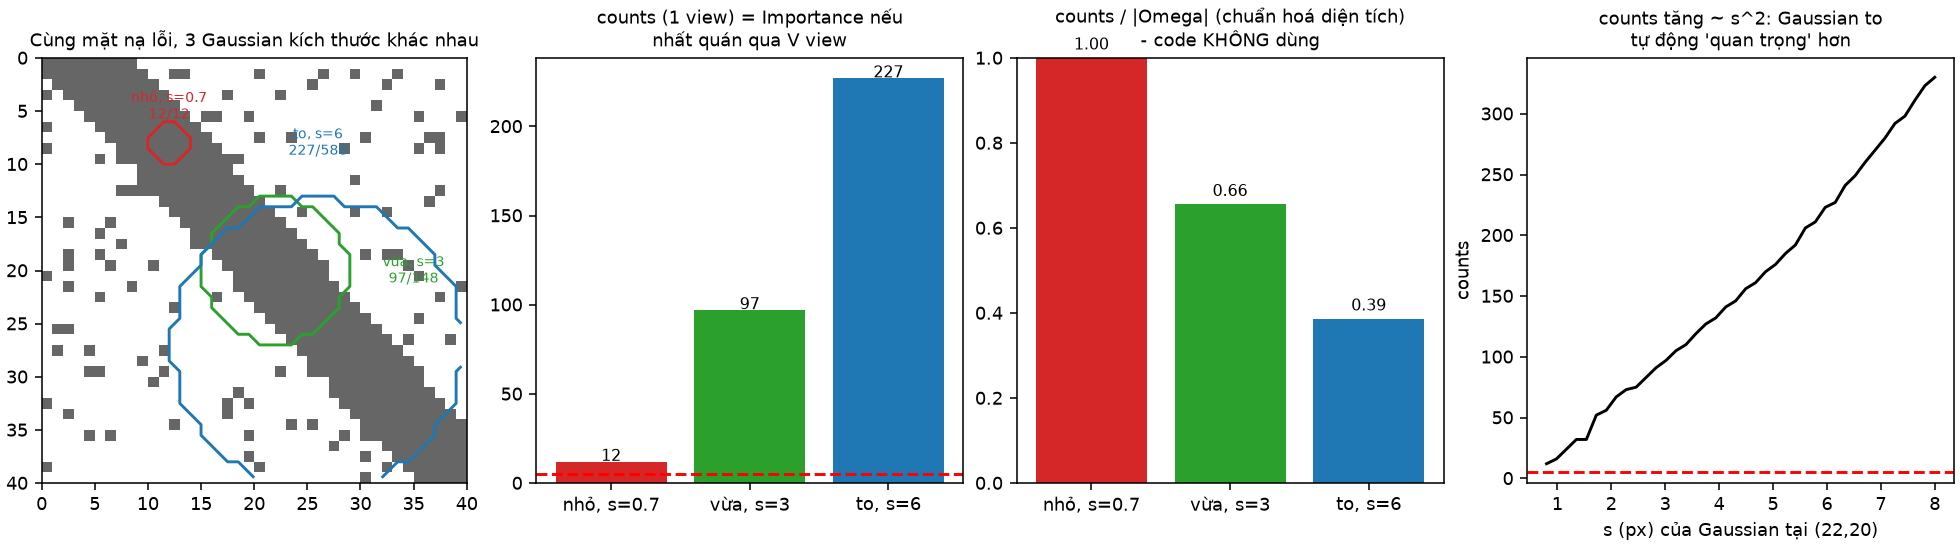
\includegraphics[width=0.95\linewidth]{2_12_to-vs-nho.png}
\captionof{figure}{\footnotesize Footprint 3 Gaussian kích thước khác nhau trên cùng mặt nạ lỗi; counts tăng $\sim s^2$.}
\end{column}
\end{columns}
\end{frame}


\section{ADC chuyên sâu — P3: Công thức Score \& Pruning}
% partADC_3a.tex --- Phan 3a: Adaptive Density Control -- E_photo va lien he voi Pruning
% 6 frame, khong documentclass/usepackage/begin{document} (duoc include tu main.tex)

% --- 3_1_ephoto-3view.png ---
\begin{frame}{Bước (6): tổng hợp sai số ảnh $E_{\text{photo}}$ qua nhiều view}
\begin{columns}[T]
\begin{column}{0.48\linewidth}
\footnotesize
\begin{itemize}
  \item Mỗi view $v$ cho ra một cặp $(L1^{(v)}, \text{SSIM}^{(v)})$ giữa ảnh render và ảnh GT.
  \item Công thức tổng hợp (code: \texttt{e\_photo}, $\lambda = 0.2$):
  \[
    E_{\text{photo}}^{(v)} = (1-\lambda)\, L1^{(v)} + \lambda\,\bigl(1 - \text{SSIM}^{(v)}\bigr)
  \]
  \item Đây chính là dạng \emph{trung bình có trọng số} giữa hai thành phần L1 và $1-\text{SSIM}$, không phải max qua view.
  \item Ví dụ 3.md (ảnh 4x4, 3 view): $L1 = (0.11125,\, 0.06,\, 0.090625)$, $\text{SSIM} = (0.72,\, 0.88,\, 0.80)$.
  \item Kết quả: $E_{\text{photo}} = (0.145,\; 0.072,\; 0.1125)$ -- view 1 (SSIM thấp nhất) đóng góp lỗi lớn nhất.
\end{itemize}
\end{column}
\begin{column}{0.5\linewidth}
\centering
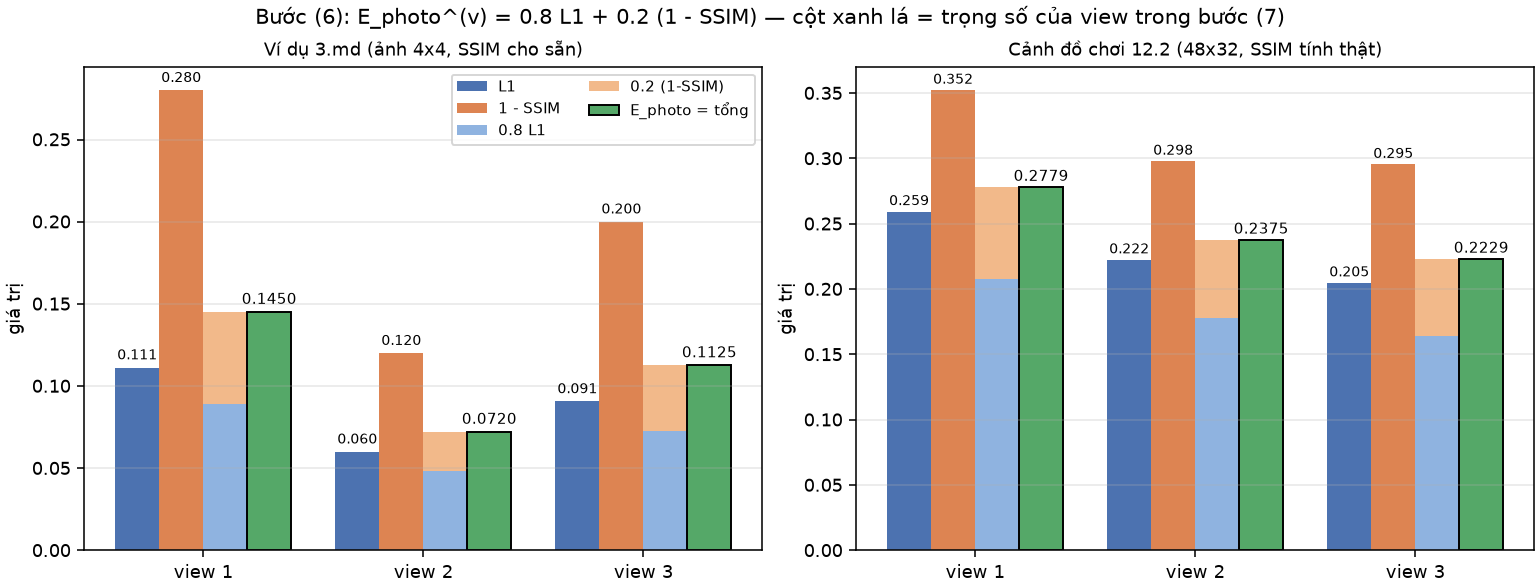
\includegraphics[width=0.95\linewidth]{3_1_ephoto-3view.png}
\captionof{figure}{\footnotesize Phân rã $E_{\text{photo}}^{(v)} = 0.8\,L1 + 0.2(1-\text{SSIM})$ cho 3 view, cột xanh lá = giá trị dùng làm trọng số ở bước (7).}
\end{column}
\end{columns}
\end{frame}

% --- 3_2_l1-vs-ssim.png ---
\begin{frame}{Vì sao cần SSIM: L1 không phân biệt được ``mờ'' và ``nhiễu''}
\begin{columns}[T]
\begin{column}{0.52\textwidth}
\scriptsize
\begin{itemize}
  \item Thí nghiệm: GT tổng hợp, Render A (blur Gaussian $\sigma{=}1.6$), Render B (nhiễu hiệu chỉnh để \textbf{cùng} $L1$ với A).
  \item $L1^{A}{\approx}L1^{B}$ nhưng cấu trúc khác $\Rightarrow \text{SSIM}^{A}{\neq}\text{SSIM}^{B}$ (blur phá cạnh giữ tương quan patch, noise phá cả hai).
  \item $\Rightarrow E_{\text{photo}}^{A}{\neq}E_{\text{photo}}^{B}$ dù $L1$ gần bằng nhau — chỉ dùng $L1$ sẽ coi hai render "lỗi như nhau".
  \item[$\Rightarrow$] $E_{\text{photo}}$ cần cả L1 (cường độ) và $1{-}$SSIM (cấu trúc, cửa sổ Gauss $11{\times}11$).
\end{itemize}
\end{column}
\begin{column}{0.48\textwidth}
\centering
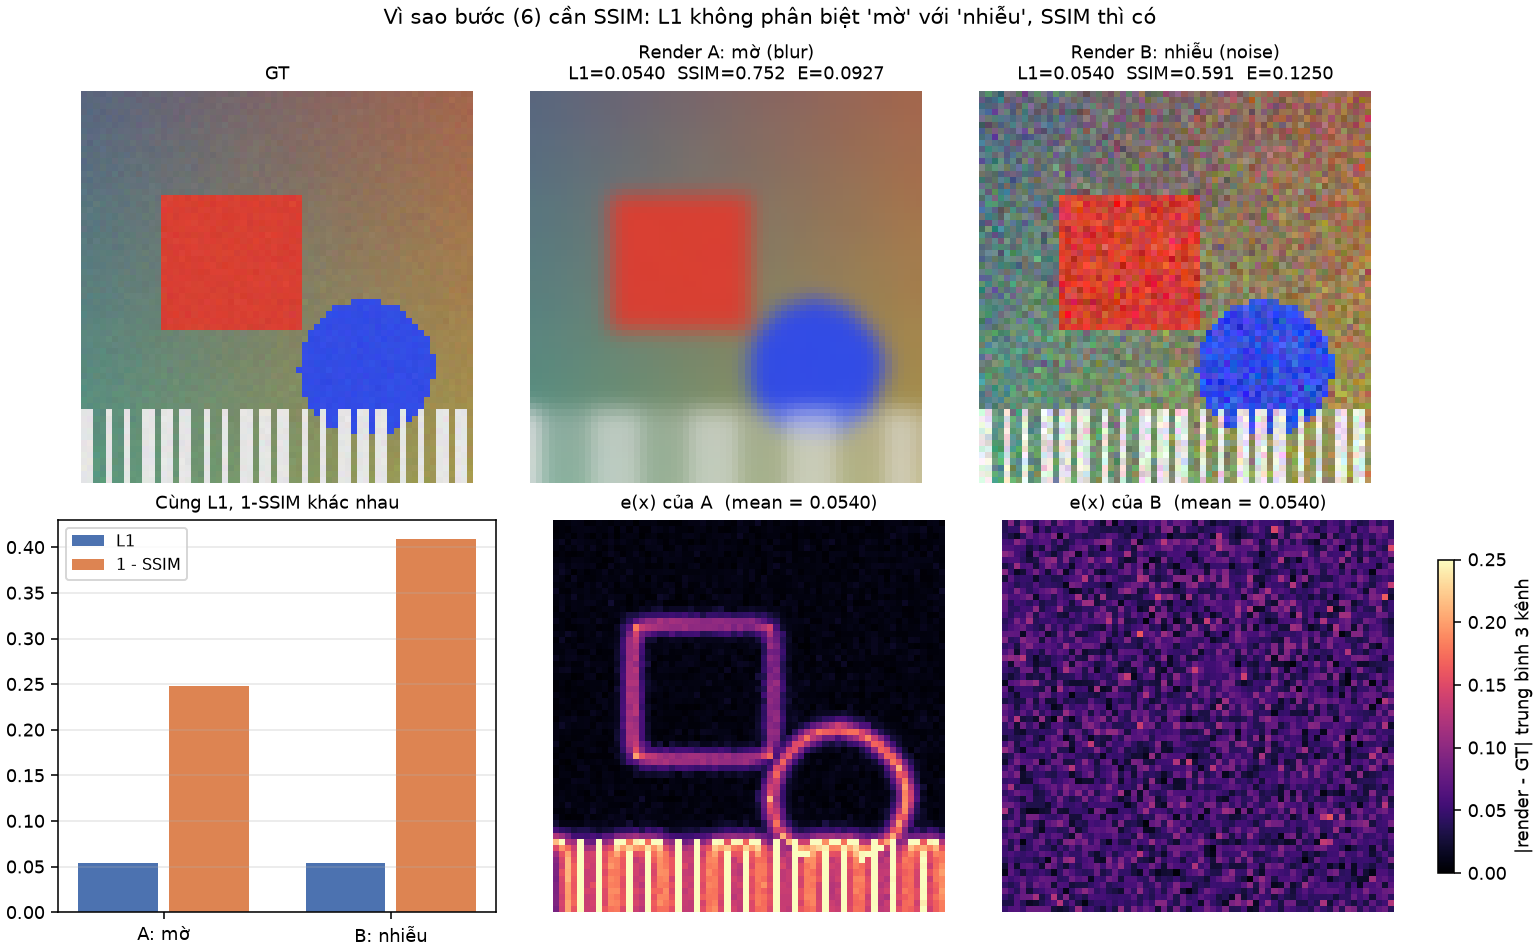
\includegraphics[width=0.95\linewidth]{3_2_l1-vs-ssim.png}
\captionof{figure}{\footnotesize Cùng $L1$, SSIM và $E_{\text{photo}}$ khác nhau giữa render mờ và nhiễu.}
\end{column}
\end{columns}
\end{frame}

% --- 3_3_ephoto-theo-lambda.png ---
\begin{frame}{$E_{\text{photo}}$ theo trọng số trộn $\lambda$}
\begin{columns}[T]
\begin{column}{0.48\linewidth}
\footnotesize
\begin{itemize}
  \item $E_{\text{photo}}^{(v)}(\lambda) = (1-\lambda)\,L1^{(v)} + \lambda\,(1-\text{SSIM}^{(v)})$ là hàm \emph{tuyến tính} theo $\lambda \in [0,1]$.
  \item $\lambda = 0$: chỉ dùng $L1$ thuần; $\lambda = 1$: chỉ dùng $1-\text{SSIM}$ (giống vai trò $\lambda_{\text{dssim}}$ trong loss huấn luyện).
  \item Giá trị mặc định trong code: $\lambda = 0.2$ -- ưu tiên L1 nhưng vẫn giữ một phần tín hiệu cấu trúc.
  \item Các đường $E_{\text{photo}}^{(v)}(\lambda)$ của từng view có thể \textbf{cắt nhau}: view có $L1$ thấp nhưng SSIM thấp có thể vượt lên khi $\lambda$ tăng.
  \item Tỉ số $E_{\max}/E_{\min}$ qua các view thay đổi rõ rệt giữa $\lambda=0$ và $\lambda=1$, cho thấy lựa chọn $\lambda$ ảnh hưởng trực tiếp đến việc view nào bị coi là ``tệ nhất''.
\end{itemize}
\end{column}
\begin{column}{0.5\linewidth}
\centering
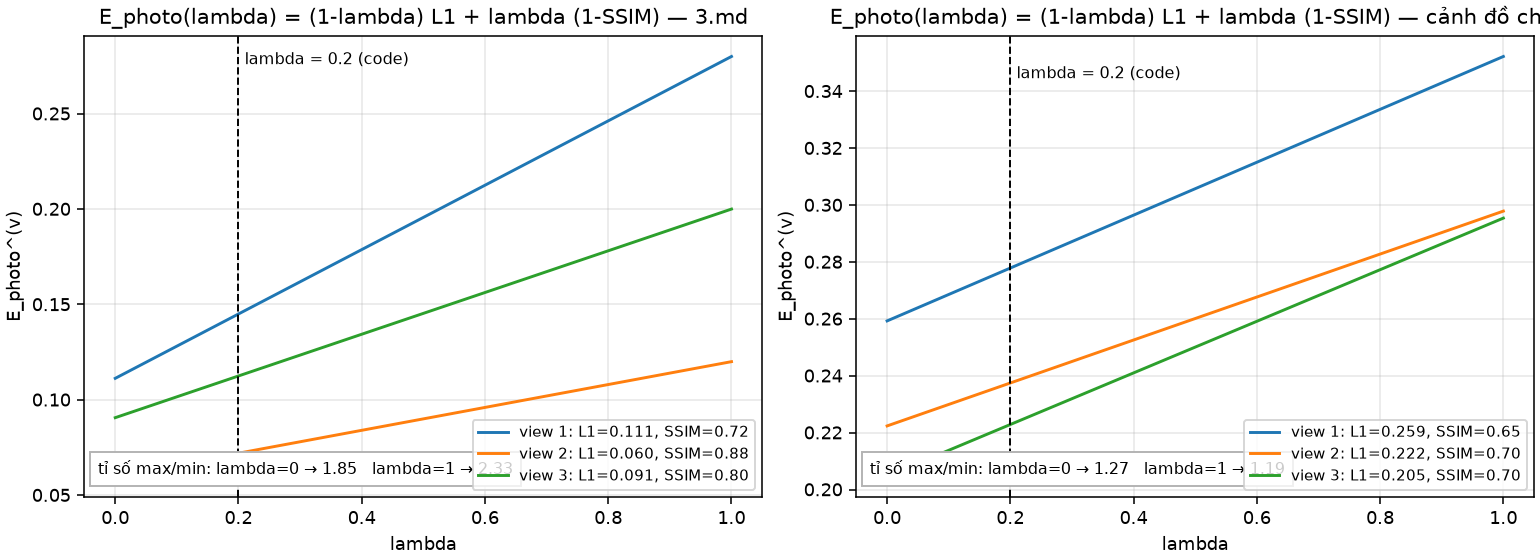
\includegraphics[width=0.95\linewidth]{3_3_ephoto-theo-lambda.png}
\captionof{figure}{\footnotesize $E_{\text{photo}}^{(v)}(\lambda)$ cho 3 view (ví dụ 3.md và cảnh đồ chơi); đường đứt nét đánh dấu $\lambda=0.2$ dùng trong code.}
\end{column}
\end{columns}
\end{frame}

% --- 3_4_heatmap-dong-gop.png ---
\begin{frame}{Đóng góp của từng Gaussian vào điểm số tổng}
\footnotesize
\begin{itemize}
  \item Với mỗi Gaussian $i$ và view $v$, \texttt{counts}$_i^{(v)}$ (bước 4) đếm số pixel lỗi mà $i$ tham gia dựng nên trong view đó.
  \item Đóng góp có trọng số vào điểm thô: $\text{contrib}_i^{(v)} = \text{counts}_i^{(v)} \cdot E_{\text{photo}}^{(v)}$.
  \item Điểm thô tích luỹ qua $V$ view: $\text{raw}_i = \sum_{v=1}^{V} \text{counts}_i^{(v)} \, E_{\text{photo}}^{(v)}$.
  \item Ví dụ 3.md: $G3$ có \texttt{counts} $=(6,6,6)$ ở cả 3 view $\Rightarrow \text{raw}_{G3} = 6(0.145+0.072+0.1125) \approx 1.98$ -- cao nhất trong 5 Gaussian, trong khi $G1$ với \texttt{counts}$=(0,0,0)$ có $\text{raw}=0$.
  \item Heatmap minh hoạ trực quan: chỉ một vài Gaussian (hàng có màu đậm) chiếm phần lớn tổng sai số ảnh, phần còn lại đóng góp gần như bằng 0.
\end{itemize}
\centering
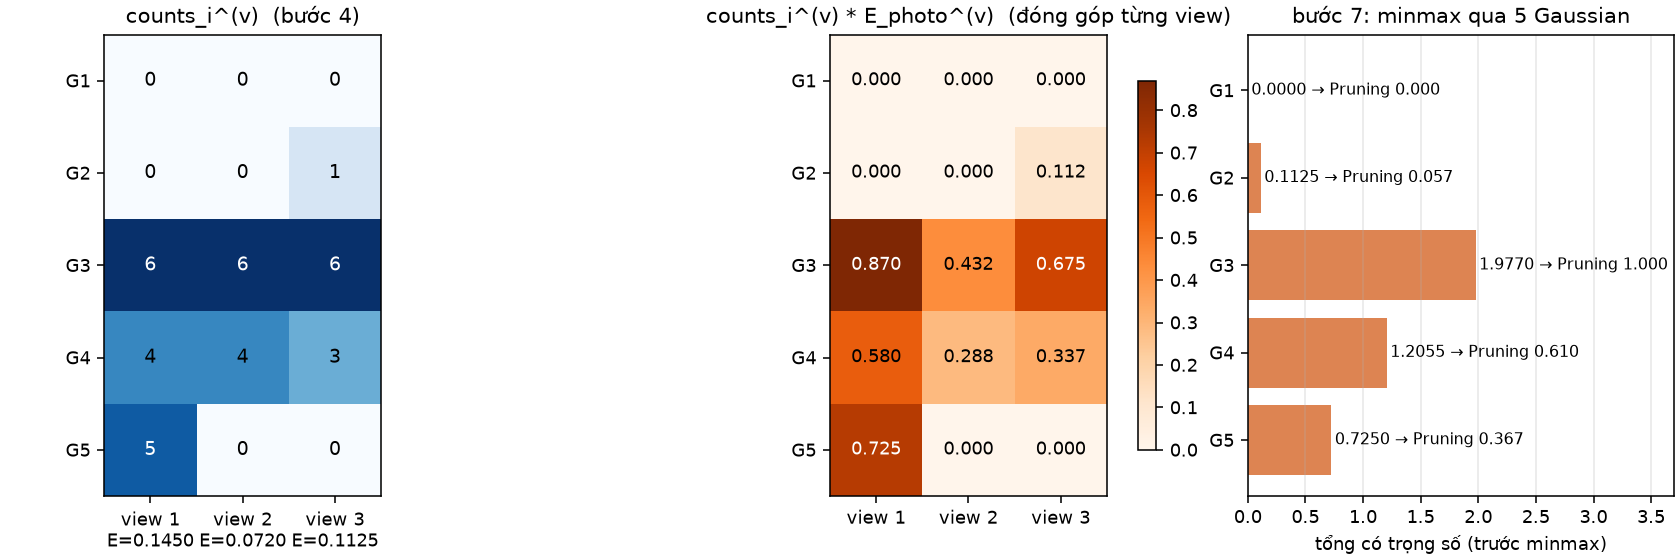
\includegraphics[width=0.85\linewidth]{3_4_heatmap-dong-gop.png}
\captionof{figure}{\footnotesize Trái: \texttt{counts}$_i^{(v)}$; giữa: đóng góp có trọng số \texttt{counts}$\cdot E_{\text{photo}}$; phải: điểm thô và Pruning sau minmax qua 5 Gaussian.}
\end{frame}

% --- 3_5_scatter-imp-pruning.png ---
\begin{frame}{Importance vs.\ Pruning: ranh giới không phải ngưỡng cứng}
\begin{columns}[T]
\begin{column}{0.48\linewidth}
\footnotesize
\begin{itemize}
  \item Importance: $\text{Importance}_i = \left\lfloor \dfrac{1}{V}\sum_{v=1}^{V} \text{counts}_i^{(v)} \right\rfloor$ -- số nguyên, dùng để quyết định \emph{densify} (ngưỡng $> 5$).
  \item Pruning: $\text{Pruning}_i = \text{minmax}_i(\text{raw}_i)$, chuẩn hoá $\text{raw}$ về $[0,1]$ qua toàn bộ $N$ Gaussian -- dùng cho \emph{final prune} (ngưỡng $>0.9$).
  \item Trên tập mô phỏng 300 Gaussian, $V{=}10$: hai đại lượng tương quan hạng dương (hệ số Spearman $\rho$ hiển thị trên hình) nhưng \textbf{không phải hàm một-một} của nhau.
  \item Với cùng một giá trị Importance, Pruning trải rộng trên một khoảng giá trị -- do Pruning còn phụ thuộc \emph{view nào} chứa lỗi (qua trọng số $E_{\text{photo}}^{(v)}$), còn Importance chỉ đếm số lượt xuất hiện.
  \item Kết luận: quyết định pruning có vùng chuyển tiếp mờ quanh ranh giới, không cắt cứng theo Importance.
\end{itemize}
\end{column}
\begin{column}{0.5\linewidth}
\centering
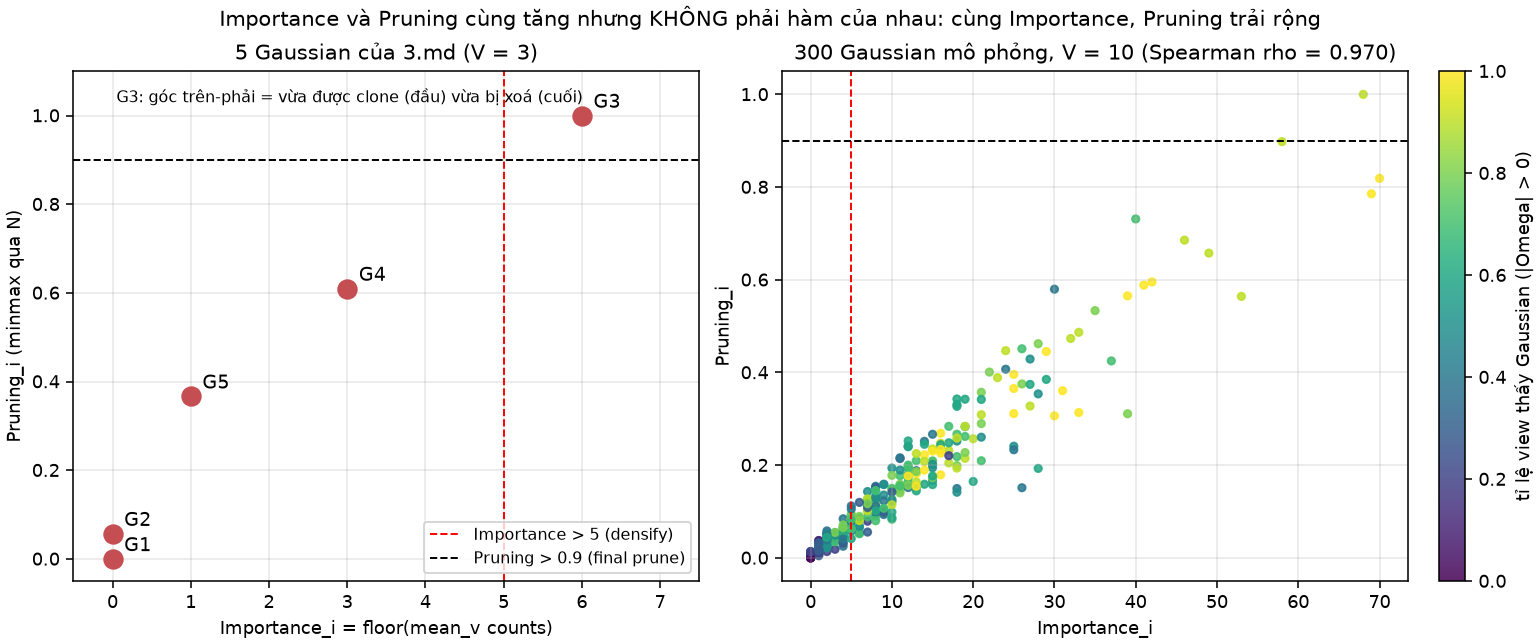
\includegraphics[width=0.95\linewidth]{3_5_scatter-imp-pruning.png}
\captionof{figure}{\footnotesize Trái: 5 Gaussian ví dụ 3.md; phải: 300 Gaussian mô phỏng, màu = tỉ lệ view thấy được Gaussian.}
\end{column}
\end{columns}
\end{frame}

% --- 3_6_pruning-vs-1-minus-imp.png ---
\begin{frame}{Pruning $\neq 1 - $ Importance chuẩn hoá}
\footnotesize
\begin{itemize}
  \item Bốn kịch bản cùng tổng \texttt{counts} nhưng phân bố khác nhau qua 3 view: A $=(6,6,6)$, B $=(18,0,0)$, C $=(0,18,0)$, D $=(17,0,0)$.
  \item A, B, C có cùng $\text{Importance} = \lfloor 18/3 \rfloor = 6$, nhưng điểm thô $\text{raw} = \sum_v \text{counts}^{(v)} E_{\text{photo}}^{(v)}$ khác nhau rõ rệt: dồn lỗi vào view có $E_{\text{photo}}$ cao (view 1, $E{=}0.145$) cho \text{raw} lớn hơn dồn vào view tốt nhất (view 2, $E{=}0.072$).
  \item D có tổng thấp hơn (17) nên Importance có thể giảm bậc trong khi raw vẫn gần B -- cho thấy việc lấy $\lfloor \cdot \rfloor$ làm mất thông tin mà Pruning (không làm tròn, có trọng số $E_{\text{photo}}$) vẫn giữ được.
  \item Trên 300 Gaussian mô phỏng: ứng với mỗi mức Importance cố định, Pruning trải trên một khoảng (thanh xám) thay vì một giá trị duy nhất.
  \item Do đó xác suất một Gaussian bị pruning tăng dần khi importance của nó giảm ($\sim 1-\text{importance}$ về xu hướng), nhưng đây là quan hệ \textbf{mang tính xác suất/thống kê}, không phải phép cắt tất định 1--1.
\end{itemize}
\centering
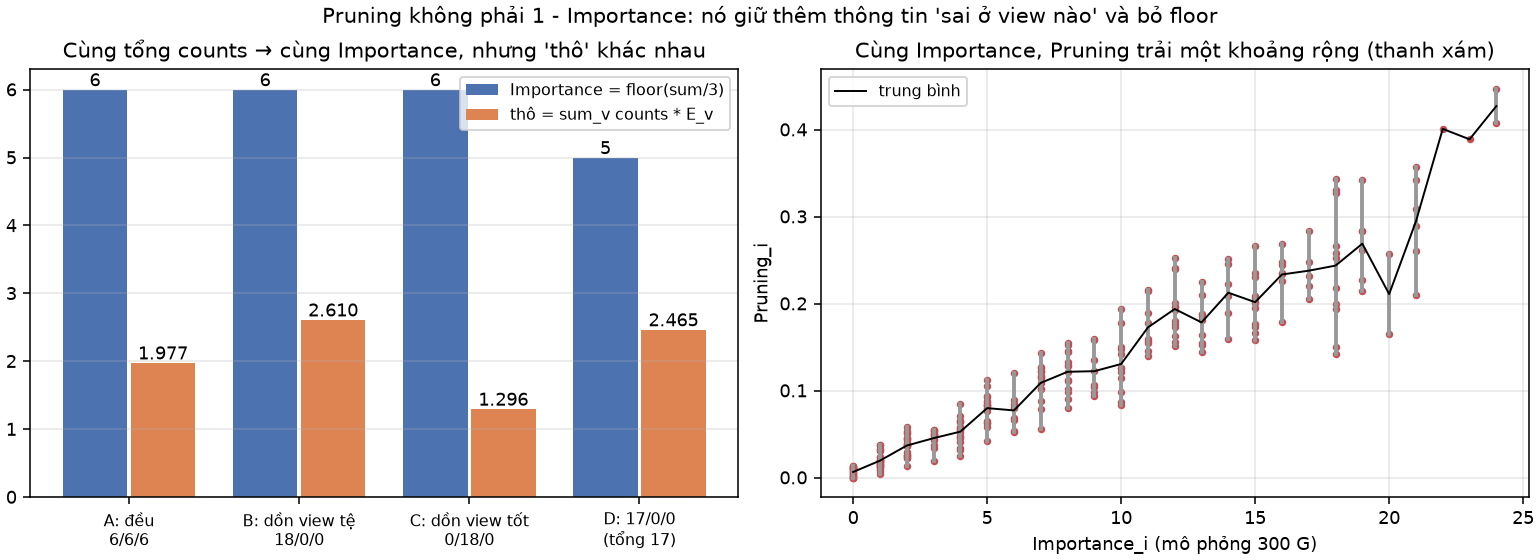
\includegraphics[width=0.78\linewidth]{3_6_pruning-vs-1-minus-imp.png}
\captionof{figure}{\footnotesize Trái: cùng Importance nhưng raw khác nhau tuỳ phân bố lỗi qua view; phải: khoảng giá trị Pruning ứng với mỗi mức Importance trên 300 Gaussian mô phỏng.}
\end{frame}

% partADC-3b: Adaptive Density Control - tong ket 7 buoc, do nhay, chi phi, outlier score
% 6 frames, khong documentclass/preamble, chi include vao main.tex

% --- 3_7_so-do-7-buoc.png ---
\begin{frame}{Tổng hợp: luồng dữ liệu 7 bước tính Importance / Pruning}
\tiny
\begin{itemize}
    \item Bước (1)--(4) trên từng view $v$: render $\to$ sai số $e_v{=}\text{mean}_{ch}|.|$ $\to$ minmax $\hat e_v$ $\to$ mặt nạ $m_v{=}\mathbb{1}[\hat e_v{>}0.1]$ $\to$ đổ về Gaussian thành $\texttt{counts}_v$.
    \item Bước (6): $E_{photo}^{(v)} = 0.8\,L1 + 0.2\,(1-\text{SSIM})$ (scalar/ảnh); tích luỹ qua $V$ view:
    $\texttt{full\_counts}{+}{=}\texttt{counts}_v,\ \texttt{full\_score}{+}{=}E_{photo}^{(v)}{\cdot}\texttt{counts}_v$
    \item Bước (5): $\text{Importance}_i{=}\lfloor \texttt{full\_counts}_i/V\rfloor \to$ densify khi $\text{Importance}_i{>}5$.
    \item Bước (7): $\text{Pruning}_i{=}\text{minmax}_i(\texttt{full\_score}) \to w_i{=}\frac{1}{10^{-6}+1-\text{Pruning}_i}$, prune khi ${>}0.9$.
    \item Độ phức tạp: $O(HW)$/view, $O(\sum_v|\Omega_v|)$ đổ về Gaussian, $O(N)$ cho (5)(7).
\end{itemize}
\centering
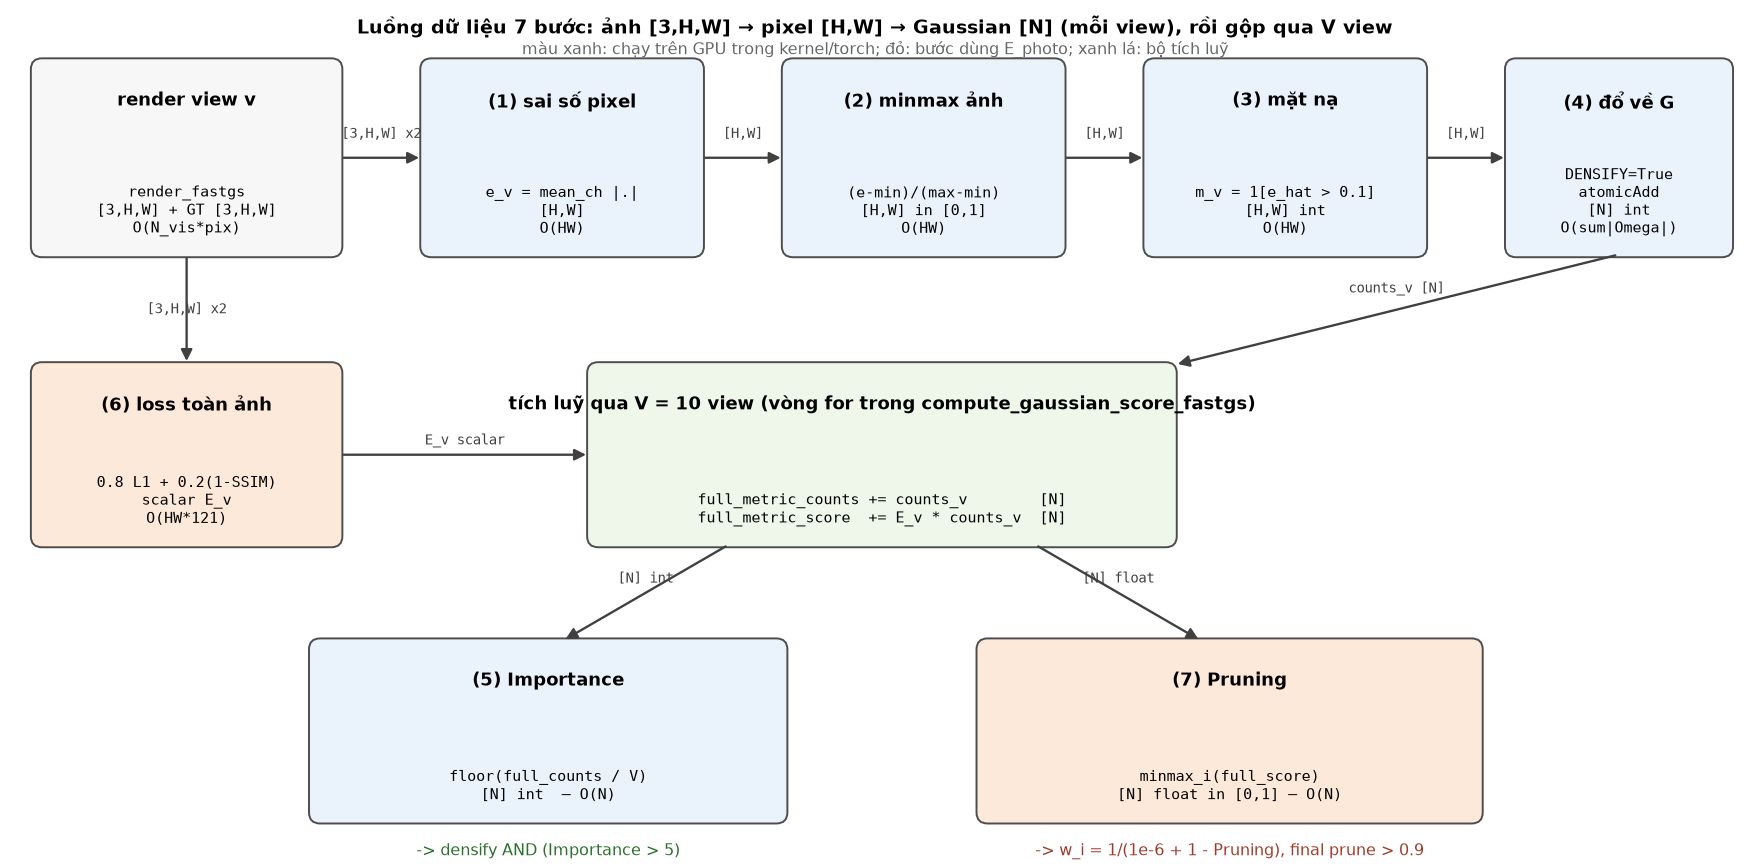
\includegraphics[width=0.55\linewidth]{3_7_so-do-7-buoc.png}
\captionof{figure}{\footnotesize Toàn cảnh 7 bước tính Importance/Pruning.}
\end{frame}

% --- 3_8_do-nhay-lambda-5g.png ---
\begin{frame}{Độ nhạy tham số $\lambda$: ví dụ 5 Gaussian (3.md)}
\begin{columns}
\begin{column}{0.55\textwidth}
\footnotesize
\begin{itemize}
    \item Quét $\lambda \in [0,1]$, tính lại $\text{Pruning}_i(\lambda)$ cho 5 Gaussian $G_1,\dots,G_5$ từ \texttt{COUNTS\_3MD} và \texttt{L1\_3MD}, \texttt{SSIM\_3MD}.
    \item Kết quả: \textbf{đổi $\lambda$ chỉ đổi giá trị Pruning, không đổi thứ hạng} trong khoảng $\lambda \in [0,1]$ -- các đường không cắt nhau.
    \item Nếu \textbf{bỏ hoàn toàn trọng số} ($E_v \equiv 1$, tức chỉ dùng \texttt{counts.sum}), thứ hạng có thể \textbf{đảo ngược}: ví dụ $G_5$ so với $G_6^{*}$ giả định (counts $=[0,6,0]$, lỗi tập trung đúng ở view \textbf{tốt nhất}) đổi chỗ cho nhau khi bỏ trọng số.
    \item Đổi cách chuẩn hoá (chia cho max, hoặc z-score) trên cùng \texttt{raw} ($\lambda=0.2$) \textbf{không đổi thứ hạng} vì đây là các phép biến đổi đơn điệu trên cùng một vector.
    \item Kết luận: công thức \textbf{ổn định với $\lambda$}, nhưng \textbf{nhạy với việc có/không có trọng số} $E_{photo}^{(v)}$ theo view.
\end{itemize}
\end{column}
\begin{column}{0.45\textwidth}
\centering
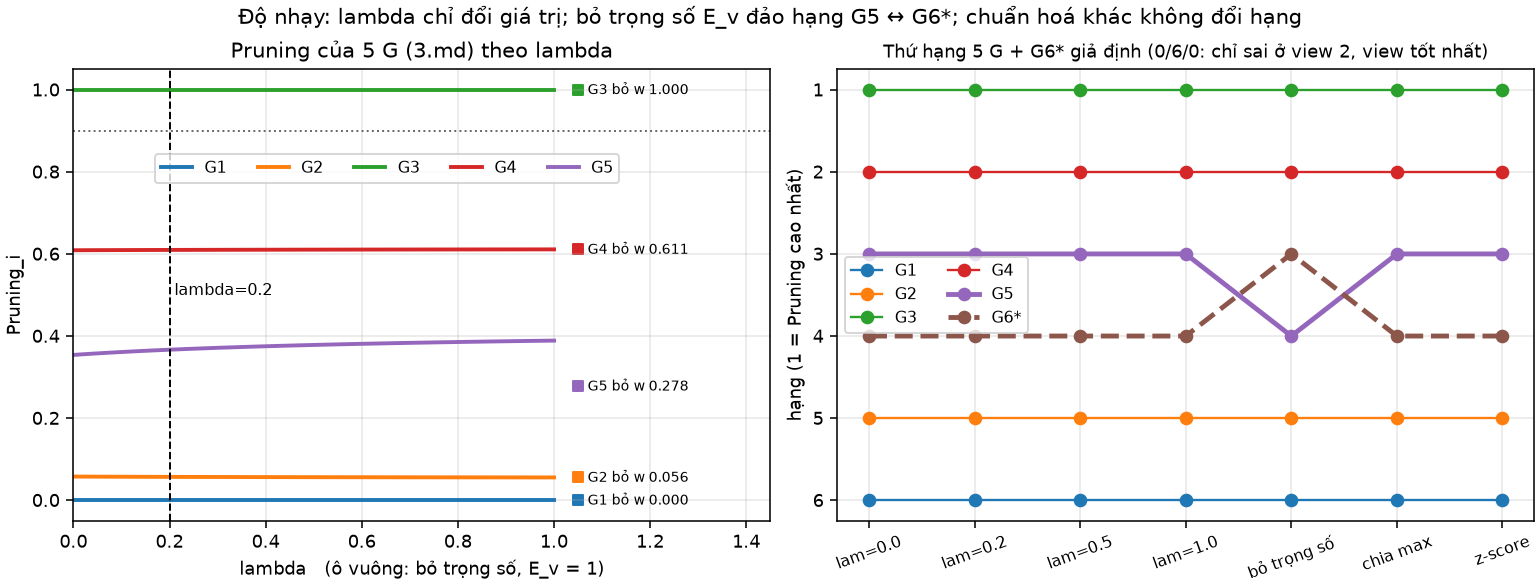
\includegraphics[width=\linewidth]{3_8_do-nhay-lambda-5g.png}
\captionof{figure}{\footnotesize Trái: $\text{Pruning}_i(\lambda)$, đường $\lambda=0.2$ (code) và $\lambda=1.05$ (bỏ trọng số). Phải: bump chart thứ hạng qua 6 liên số, gồm $G_6^{*}$.}
\end{column}
\end{columns}
\end{frame}

% --- 3_9_rank-change-300g.png ---
\begin{frame}{Kiểm tra tính robust ở quy mô lớn: 300 Gaussian mô phỏng}
\begin{columns}[T]
\begin{column}{0.52\textwidth}
\scriptsize
Mô phỏng $N{=}300$, $V{=}10$ view, so thứ hạng $\text{Pruning}_i$ gốc ($\lambda{=}0.2$) với biến thể:
\begin{itemize}
    \item $\lambda{=}0$: \textbf{0.0\%} đổi hạng, tập $>0.9$ giữ \textbf{100\%}.
    \item $\lambda{=}1$: \textbf{2.3\%} đổi hạng, vẫn giữ \textbf{100\%}.
    \item Bỏ trọng số ($E_v{\equiv}1$): \textbf{37.3\%} đổi hạng — lớn nhất — tập $>0.9$ chỉ còn \textbf{99.3\%}.
    \item Thay $E_v$ bằng $\text{rank}(E_v)$: chỉ \textbf{3.7\%} đổi hạng.
    \item $E_{photo}$ giữa 10 view: max/min${=}5.61$.
\end{itemize}
\end{column}
\begin{column}{0.48\textwidth}
\centering
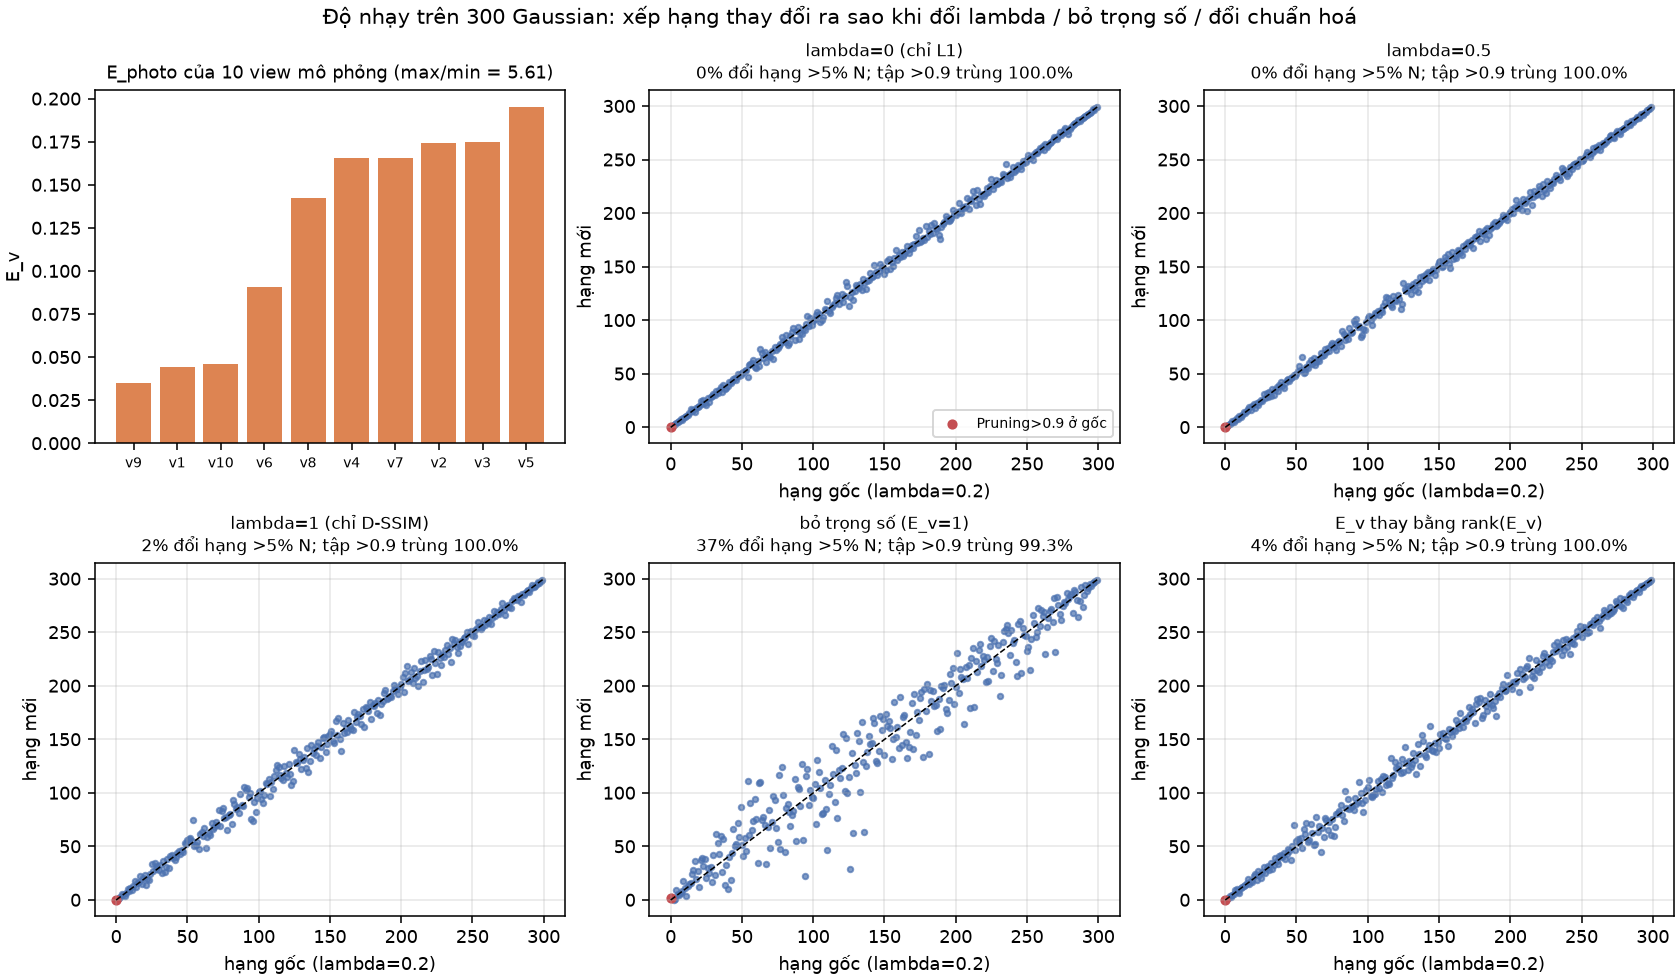
\includegraphics[width=0.95\linewidth]{3_9_rank-change-300g.png}
\captionof{figure}{\footnotesize Hạng gốc vs biến thể; đỏ = Gaussian trong $\text{Pruning}>0.9$ gốc.}
\end{column}
\end{columns}
\end{frame}

% --- 3_10_chi-phi-scoring.png ---
\begin{frame}{Chi phí tính toán của bước scoring có là nút thắt mới?}
\begin{columns}
\begin{column}{0.52\textwidth}
\footnotesize
\begin{itemize}
    \item Thiết lập: \texttt{densify\_from\_iter}$=500$, \texttt{densify\_until\_iter}$=15000$, tổng \texttt{iterations}$=30000$; mỗi lần densify cần \textbf{thêm} $10$ view $\times$ $2$ lần render (GT + mới) $= 20$ forward-equivalent.
    \item Interval $=500$: $n_{densify}=28$ lần $\to +560$ forward. So với train ($1$ vòng $\approx 3$ forward-equivalent, tổng $90000$): overhead $\mathbf{0{,}62\%}$ (cận trên nếu $1$ vòng $=1$ forward: $1{,}87\%$).
    \item Interval $=200$: $n_{densify}=72$ lần $\to +1440$ forward $\to$ overhead $\mathbf{1{,}6\%}$ (cận trên $4{,}8\%$).
    \item Interval $=100$: $n_{densify}=144$ lần $\to +2880$ forward $\to$ overhead $\mathbf{3{,}2\%}$ (cận trên $9{,}6\%$).
    \item Overhead $\sim 1/\text{interval}$ -- ngay cả interval nhỏ nhất thường dùng ($100$), scoring vẫn dưới $10\%$ tổng chi phí train $\to$ \textbf{không} phải nút thắt mới.
\end{itemize}
\end{column}
\begin{column}{0.48\textwidth}
\centering
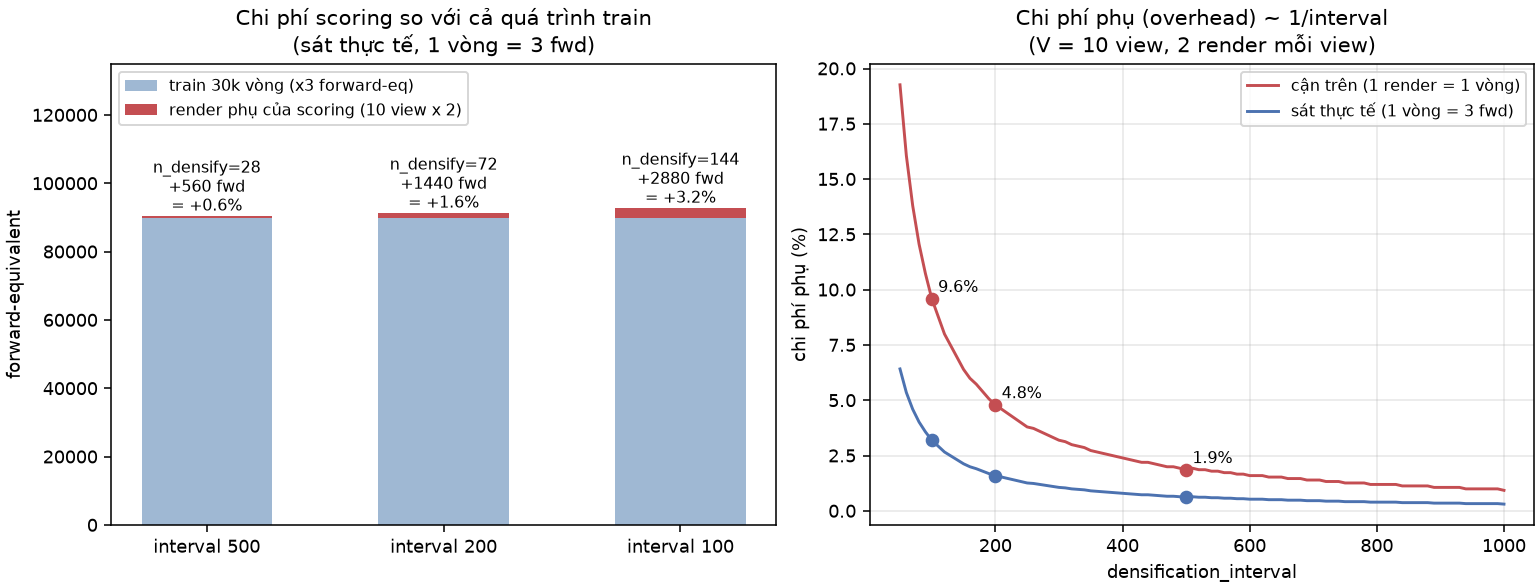
\includegraphics[width=\linewidth]{3_10_chi-phi-scoring.png}
\captionof{figure}{\footnotesize Trái: chồng bar train vs scoring theo interval. Phải: overhead (\%) theo interval, hai đường cận trên / sát thực tế.}
\end{column}
\end{columns}
\end{frame}

% --- 3_11_pruning-to-w.png ---
\begin{frame}{Từ điểm số đến trọng số lấy mẫu $w_i$ (bước chuẩn bị cho Phần 5)}
\footnotesize
\begin{itemize}
    \item Công thức chuyển đổi ($\S7.4$): $\displaystyle w_i = \frac{1}{10^{-6} + 1 - \text{Pruning}_i}$ -- $w_i$ tăng \textbf{siêu tuyến tính} và \textbf{phân kỳ} khi $\text{Pruning}_i \to 1$.
    \item Ví dụ 3.md: $\text{Pruning} = [0,\ 0{,}057,\ 1{,}0,\ 0{,}610,\ 0{,}367]$ cho $G_1,\dots,G_5$ $\Rightarrow$ $w = [1{,}0,\ 1{,}06,\ 10^{6},\ 2{,}56,\ 1{,}58]$ (dùng $10^{-6}$ trong mẫu để tránh chia cho 0 khi $\text{Pruning}=1$).
    \item Chuẩn hoá thành xác suất lấy mẫu $p_i = w_i / \sum_j w_j$: $G_3$ chiếm $p_{G_3} \approx 0{,}999994$ ($\approx 100\%$) xác suất ở lượt rút mẫu đầu tiên -- các Gaussian còn lại gần như \textbf{không bao giờ được chọn}.
    \item Cảnh đồ chơi (4 Gaussian): $\text{Pruning} = [0{,}7654,\ 0{,}4507,\ 1{,}0,\ 0{,}0]$ -- vẫn có một Gaussian đạt $\text{Pruning}=1$ gây $w \to \infty$.
    \item Ngưỡng tuyệt đối $\text{Pruning}>0.9$ (prune cuối) độc lập với công thức $w_i$, nhưng cả hai đều nhạy với cùng một đại lượng: giá trị cực đại của \texttt{full\_score}.
\end{itemize}
\begin{center}
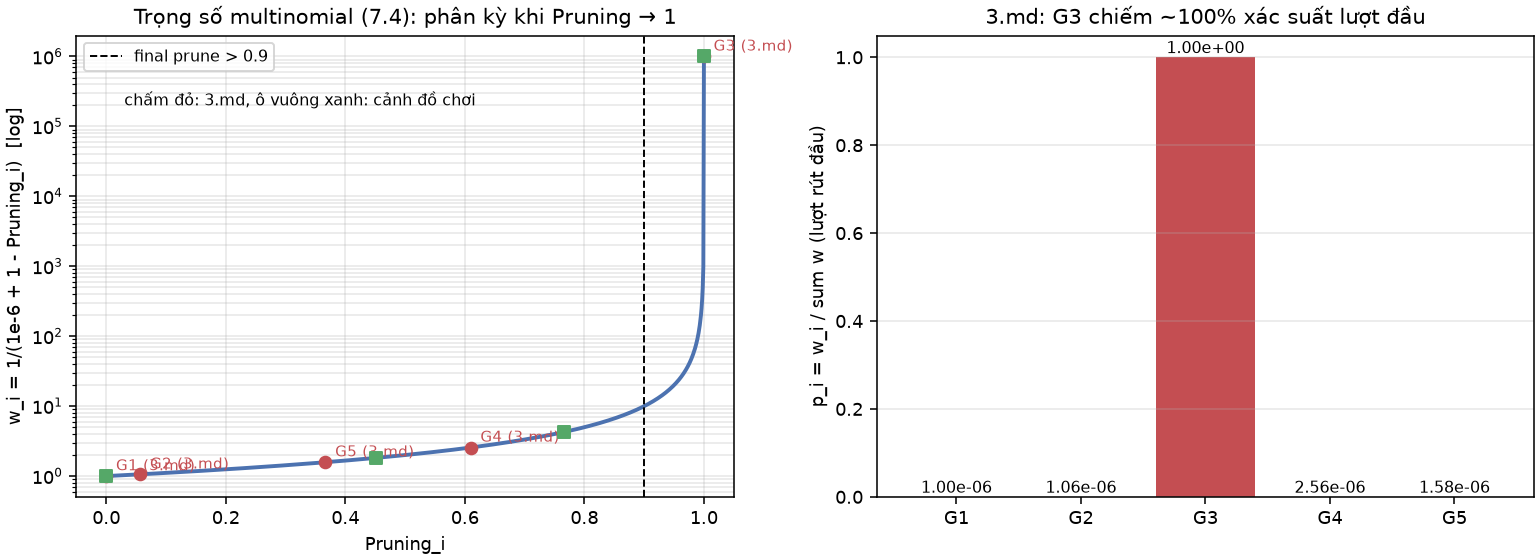
\includegraphics[width=0.68\linewidth]{3_11_pruning-to-w.png}
\captionof{figure}{\footnotesize Trái: $w(\text{Pruning})$ (thang log), các Gaussian 3.md/đồ chơi đánh dấu. Phải: $p_i$ cho 3.md -- $G_3$ chi phối hoàn toàn.}
\end{center}
\end{frame}

% --- 3_12_minmax-outlier.png ---
\begin{frame}{Outlier trong chính điểm SCORE tổng hợp -- lặp lại vấn đề từ Phần 1}
\footnotesize
\begin{itemize}
    \item Nhắc lại Phần 1: min-max $\dfrac{x-\min}{\max-\min}$ nhạy với outlier ở \textbf{cả hai đầu}; ở đây áp dụng cho \texttt{raw\_score} $= \sum_v \texttt{counts}_v \cdot E_{photo}^{(v)}$ trước khi lấy minmax thành Pruning.
    \item Thí nghiệm: quần thể $300$ Gaussian mô phỏng, nhân giá trị \texttt{raw} lớn nhất lên $\times 3$ (một Gaussian sai rất nặng xuất hiện thêm).
    \item Trước outlier: $1$ Gaussian có $\text{Pruning}>0.9$, $13$ Gaussian có $\text{Pruning}>0.5$.
    \item Sau khi thêm outlier: vẫn chỉ $1$ Gaussian có $\text{Pruning}>0.9$ (chính nó), nhưng số Gaussian có $\text{Pruning}>0.5$ \textbf{giảm mạnh từ 13 xuống còn 1} -- toàn bộ quần thể còn lại bị kéo dồn về gần $0$.
    \item Thứ hạng vẫn đơn điệu (giữ nguyên quan hệ thứ tự) vì minmax là phép biến đổi tuyến tính, nhưng \textbf{ngưỡng tuyệt đối} ($0.9$, $0.5$) và do đó \textbf{trọng số lấy mẫu} $w_i$ ở slide trước đều bị méo bởi một Gaussian duy nhất.
\end{itemize}
\begin{center}
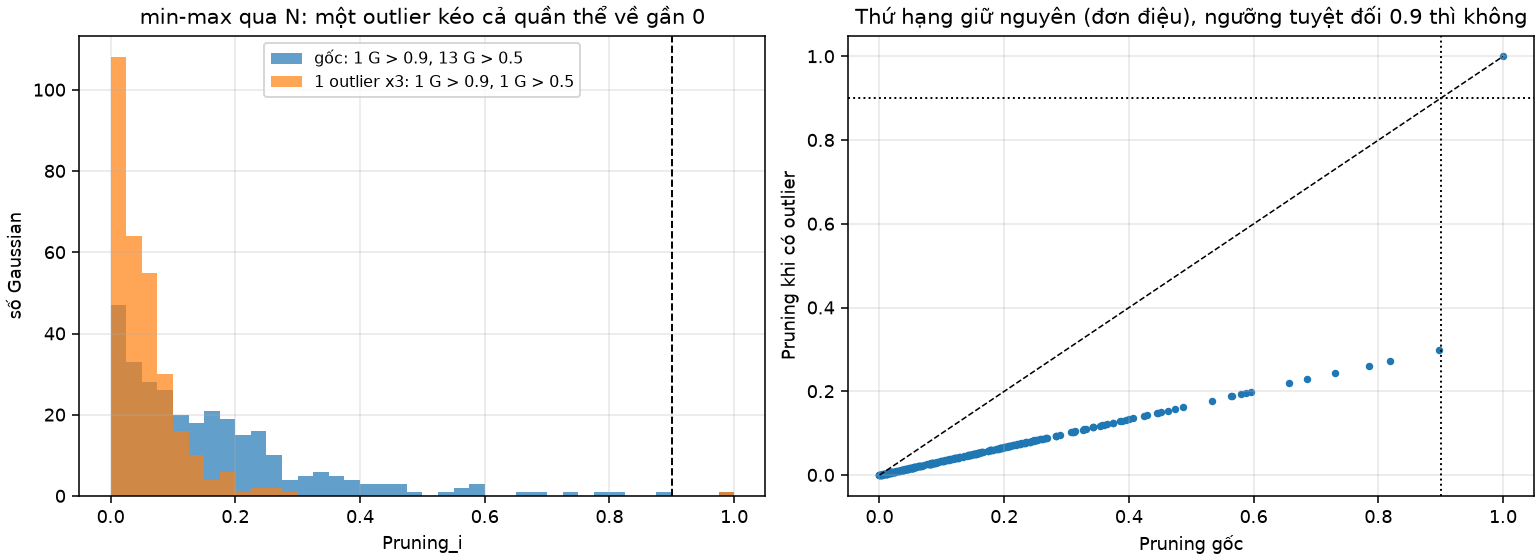
\includegraphics[width=0.68\linewidth]{3_12_minmax-outlier.png}
\captionof{figure}{\footnotesize Trái: phân bố Pruning trước/sau outlier ($\times 3$). Phải: Pruning gốc vs Pruning có outlier -- thứ hạng giữ nguyên, giá trị tuyệt đối thì không.}
\end{center}
\end{frame}


\section{ADC chuyên sâu — P4: Gradient Cancellation \& Quyết định Clone/Split}
% ============================================================
% Phần 4a — Adaptive Density Control: Gradient truyền thống,
% tích luỹ, và ranh giới quyết định clone/split (FastGS-lite)
% Nguồn số liệu: DOCS/BOOK/adc_figures/part4_figures.py
% ============================================================

% --- 4_1_gradient-cancellation.png ---
\begin{frame}{Triệt tiêu Gradient (Gradient Cancellation)}
\begin{columns}[T]
\begin{column}{0.52\linewidth}
\footnotesize
\begin{itemize}
  \item \textbf{Tầng 1 (trong 1 ảnh):} gradient vị trí theo trục $u$ đổi dấu hai bên biên vật thể $\Rightarrow$ cộng có dấu có thể gần 0; cần cột trị tuyệt đối để giữ tín hiệu.
  \item \textbf{Tầng 2 (giữa các view):} mỗi view $v$ cho một vector gradient vị trí $g^{(v)} \in \mathbb{R}^2$ hướng khác nhau.
  \item Ví dụ 4 view, góc $(20^\circ, 110^\circ, 200^\circ, 290^\circ)$, độ lớn $(1.0, 0.9, 1.1, 0.95)$:
  \[
    \Big\| \sum_{v} g^{(v)} \Big\| \approx 0.11 \quad \text{(gần 0 — SAI nếu cộng vector)}
  \]
  \item Code \texttt{add\_densification\_stats} lấy $\|g^{(v)}\|$ \textbf{TRƯỚC} rồi mới cộng qua các iteration:
  \[
    \texttt{accum} = \sum_v \|g^{(v)}\| = 3.95, \quad
    \bar g = \frac{\texttt{accum}}{\texttt{denom}} = \frac{3.95}{4} = 0.9875
  \]
  \item Kết luận: chuẩn hoá bằng norm-trước-rồi-cộng tránh triệt tiêu, còn cộng vector trực tiếp gần như xoá sạch tín hiệu densify.
\end{itemize}
\end{column}
\begin{column}{0.46\linewidth}
\centering
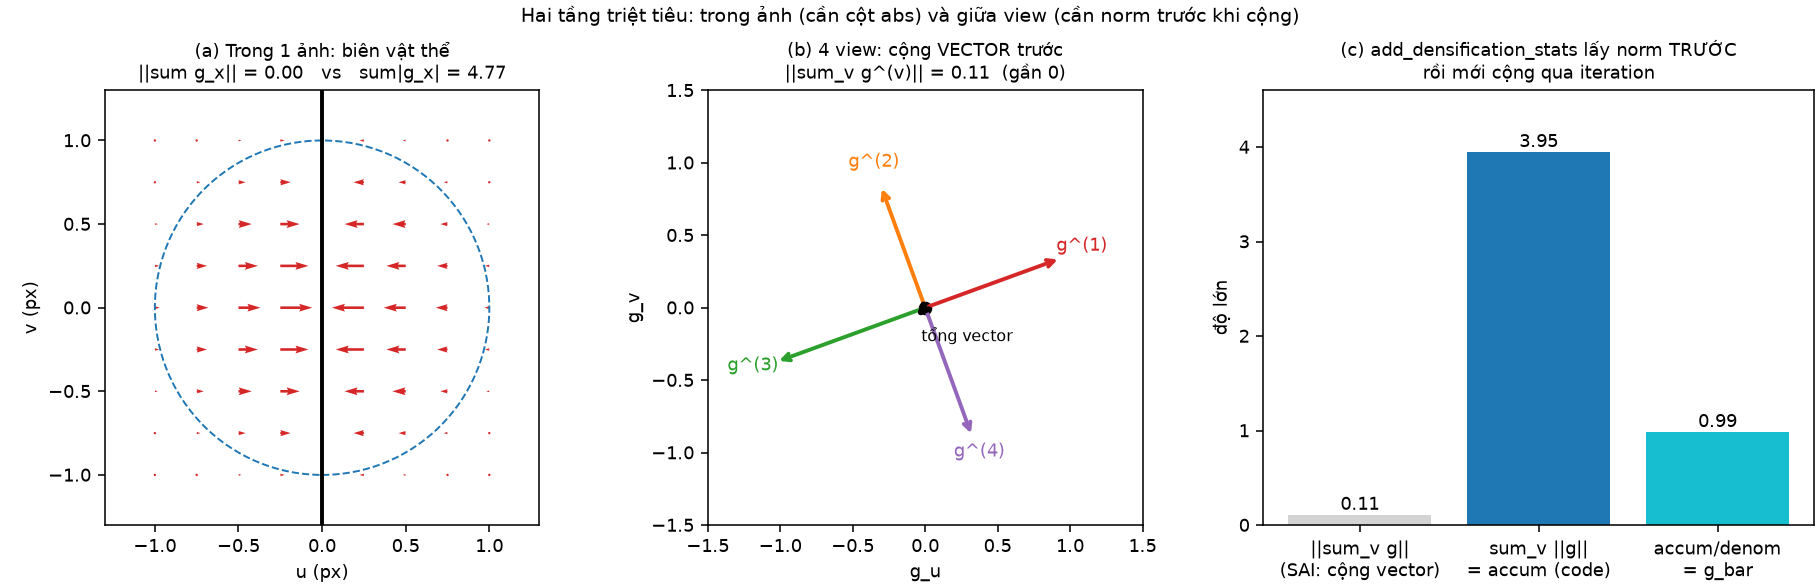
\includegraphics[width=0.95\linewidth]{4_1_gradient-cancellation.png}
\captionof{figure}{\footnotesize Hai tầng triệt tiêu: trong ảnh (cần abs) và giữa view (cần norm trước khi cộng).}
\end{column}
\end{columns}
\end{frame}

% --- 4_2_accum-denom-curve.png ---
\begin{frame}{Đường cong tích luỹ: accum, denom, $\bar g$}
\begin{columns}[T]
\begin{column}{0.5\linewidth}
\footnotesize
\begin{itemize}
  \item Trong 1 chu kỳ \texttt{densification\_interval} $T=100$ vòng lặp, mỗi Gaussian tích luỹ:
  \[
    \texttt{accum}_t = \sum_{t'\le t, \text{visible}} \|g_{t'}\|, \qquad
    \texttt{denom}_t = \#\{t' \le t : \text{visible}\}
  \]
  \[
    \bar g_t = \frac{\texttt{accum}_t}{\texttt{denom}_t}
  \]
  \item Ba Gaussian mô phỏng: A (luôn hữu hình, $g \sim \mathcal{N}(3\times10^{-4}, 8\times10^{-5})$), B (hữu hình 40\% view, $g \sim \mathcal{N}(6\times10^{-4}, 1.5\times10^{-4})$), C (đã hội tụ, $g \sim \mathcal{N}(5\times10^{-5}, 2\times10^{-5})$).
  \item Ngưỡng $\tau_{\text{grad}} = 2\times10^{-4}$ (\texttt{--grad\_thresh}).
  \item B có \texttt{denom} nhỏ hơn A nhưng $\bar g$ vẫn cao hơn ngưỡng, vì chia theo \textbf{số lần THẤY} chứ không phải theo tổng số iteration.
  \item C có $\bar g \approx 5\times10^{-5} < \tau_{\text{grad}}$: không densify — tín hiệu tin cậy phụ thuộc \texttt{denom}, không chỉ \texttt{accum}.
\end{itemize}
\end{column}
\begin{column}{0.48\linewidth}
\centering
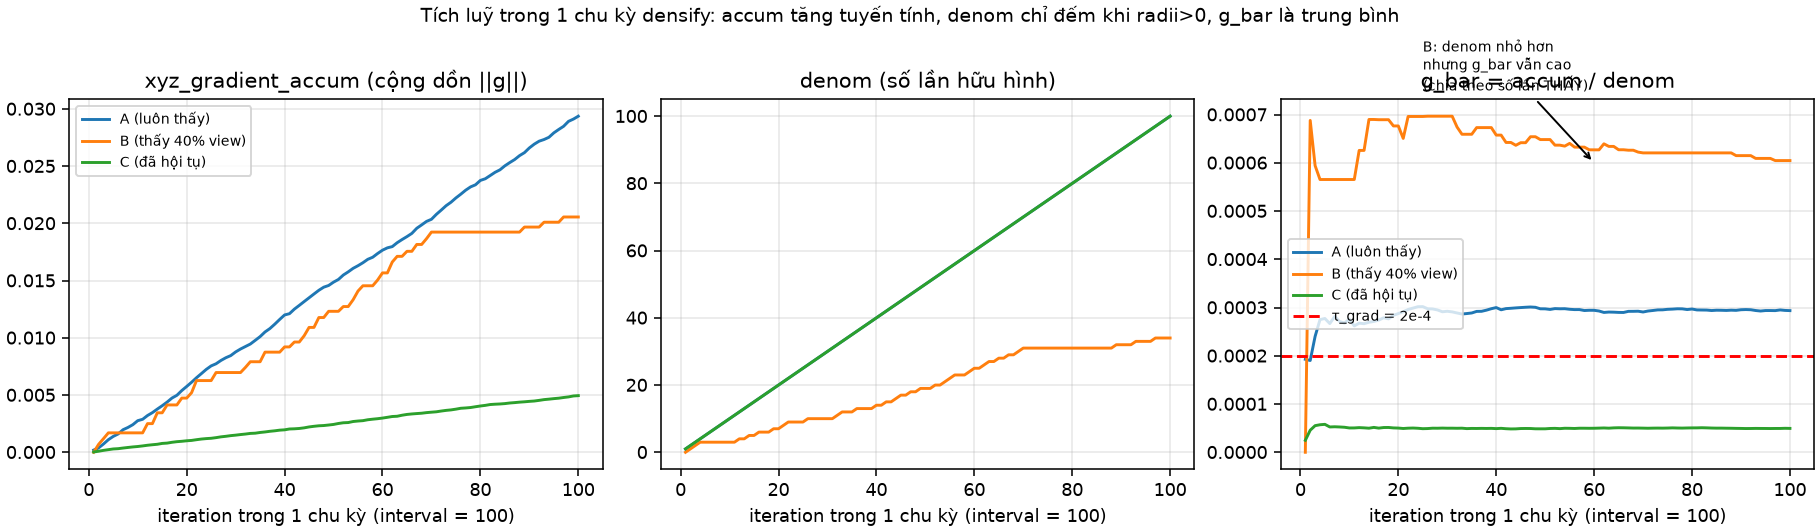
\includegraphics[width=0.95\linewidth]{4_2_accum-denom-curve.png}
\captionof{figure}{\footnotesize accum tăng tuyến tính, denom chỉ đếm khi radii\textgreater0, $\bar g$ là trung bình theo lần thấy.}
\end{column}
\end{columns}
\end{frame}

% --- 4_3_and-plane-5gaussians.png ---
\begin{frame}{Mặt phẳng AND: gradient truyền thống $\times$ Importance}
\footnotesize
\begin{columns}[T]
\begin{column}{0.55\linewidth}
\begin{itemize}
  \item 5 Gaussian ví dụ (Phần 3): $\bar g = (0.00025, 0.00008, 0.00031, 0.00011, 0.00042)$, $\bar g_{\text{abs}} = (0.00040, 0.00030, 0.00055, 0.00150, 0.00070)$, Importance $= (0, 0, 6, 3, 1)$.
  \item Ngưỡng: $\tau_{\text{grad}} = 2\times10^{-4}$, $\tau_{\text{abs}} = 1.2\times10^{-3}$, ngưỡng Importance $= 5$.
  \item \textbf{Nhánh clone} (kích thước nhỏ, G1, G2, G3, G5):
  \begin{itemize}
    \footnotesize
    \item G3: $\bar g = 3.1\times10^{-4} \ge \tau_{\text{grad}}$ \textbf{AND} Imp $= 6 > 5$ $\Rightarrow$ \textbf{CLONE}.
    \item G1: $\bar g = 2.5\times10^{-4} \ge \tau_{\text{grad}}$ nhưng Imp $= 0 \le 5$ $\Rightarrow$ 3DGS gốc sẽ clone, FastGS \textbf{chặn}.
    \item G5: $\bar g = 4.2\times10^{-4} \ge \tau_{\text{grad}}$ nhưng Imp $= 1 \le 5$ $\Rightarrow$ \textbf{chặn}.
    \item G2: $\bar g = 0.8\times10^{-4} < \tau_{\text{grad}}$ $\Rightarrow$ không đạt điều kiện gradient.
  \end{itemize}
  \item \textbf{Nhánh split} (kích thước lớn, G4): $\bar g_{\text{abs}} = 1.5\times10^{-3} \ge \tau_{\text{abs}}$ nhưng Imp $= 3 \le 5$ $\Rightarrow$ \textbf{chặn}.
  \item Kết quả AND: chỉ G3 được densify (clone); G1, G5, G4 bị chặn dù gradient 3DGS gốc đạt ngưỡng.
\end{itemize}
\end{column}
\begin{column}{0.42\linewidth}
\centering
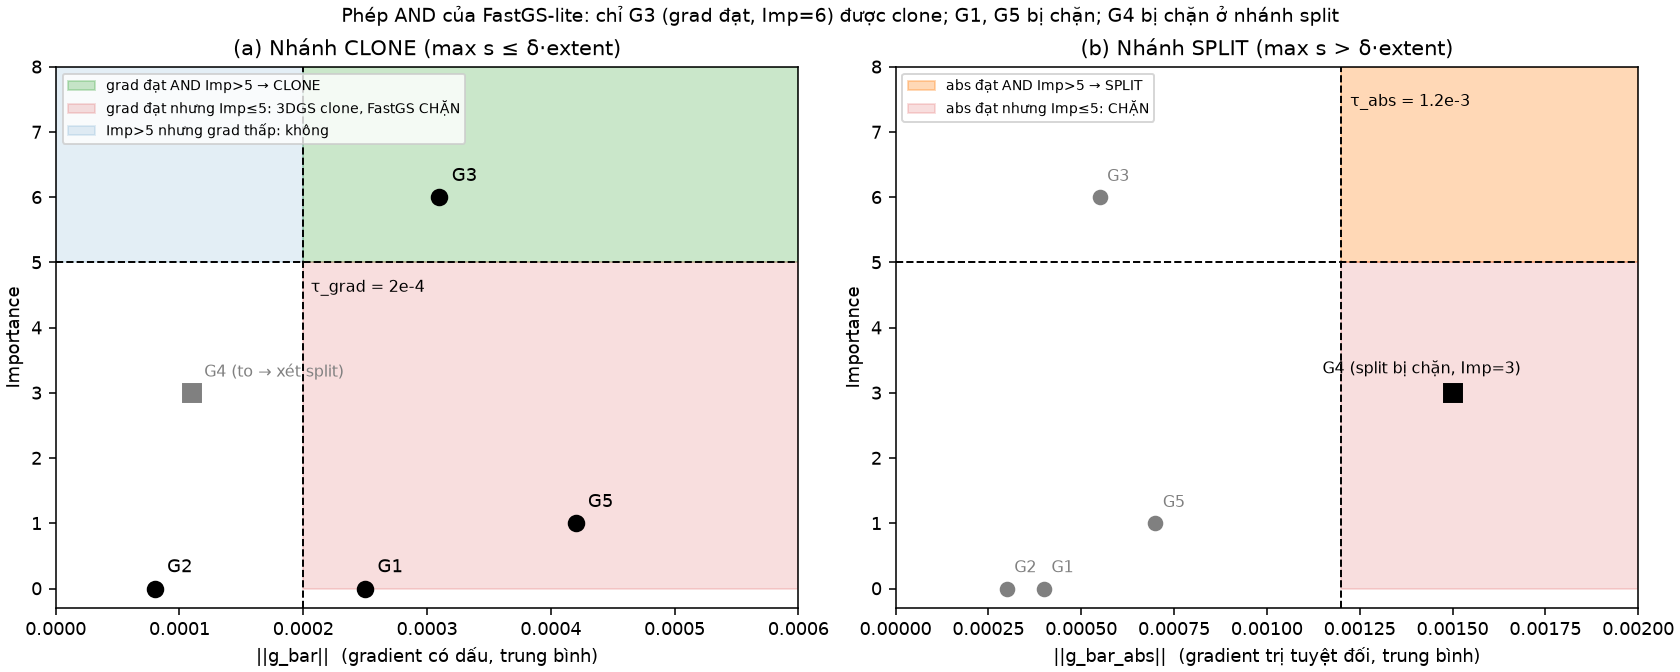
\includegraphics[width=\linewidth]{4_3_and-plane-5gaussians.png}
\captionof{figure}{\footnotesize Phép AND của FastGS-lite trên 5 Gaussian: chỉ G3 vượt cả hai điều kiện.}
\end{column}
\end{columns}
\end{frame}

% --- 4_4_clone-region-500.png ---
\begin{frame}{Vùng ứng viên clone trên quy mô 500 Gaussian}
\begin{columns}[T]
\begin{column}{0.5\linewidth}
\footnotesize
\begin{itemize}
  \item Mô phỏng $N = 500$ Gaussian, scene extent $= 1.69025$, ngưỡng kích thước $\delta \cdot \text{extent} = 0.001 \times 1.69025 = 0.00169$ (\texttt{--dense}).
  \item Điều kiện: \texttt{small} $= (\max s_i \le \delta\cdot\text{extent})$, \texttt{grad\_ok} $= (\bar g_i \ge \tau_{\text{grad}})$, \texttt{abs\_ok} $= (\bar g_{\text{abs},i} \ge \tau_{\text{abs}})$, \texttt{imp\_ok} $= (\text{Imp}_i > 5)$.
  \[
    \texttt{clone}_{\text{3DGS}} = \texttt{small} \wedge \texttt{grad\_ok}, \quad
    \texttt{clone}_{\text{FastGS}} = \texttt{clone}_{\text{3DGS}} \wedge \texttt{imp\_ok}
  \]
  \item Trên mặt phẳng $(\bar g, \max s_i)$ (trục log): vùng dưới ngưỡng kích thước và bên phải $\tau_{\text{grad}}$ là ứng viên clone của 3DGS gốc.
  \item Với Importance $\sim \mathcal{U}\{0,\dots,11\}$: phép AND chỉ giữ lại khoảng \textbf{một nửa} số ứng viên gradient — phần còn lại bị đánh dấu "3DGS densify, FastGS chặn" (Imp $\le 5$).
  \item Phân bố không gian: ứng viên clone tập trung ở vùng $\bar g$ lớn và $\max s_i$ nhỏ, tách biệt rõ với vùng split ($\max s_i$ lớn).
\end{itemize}
\end{column}
\begin{column}{0.48\linewidth}
\centering
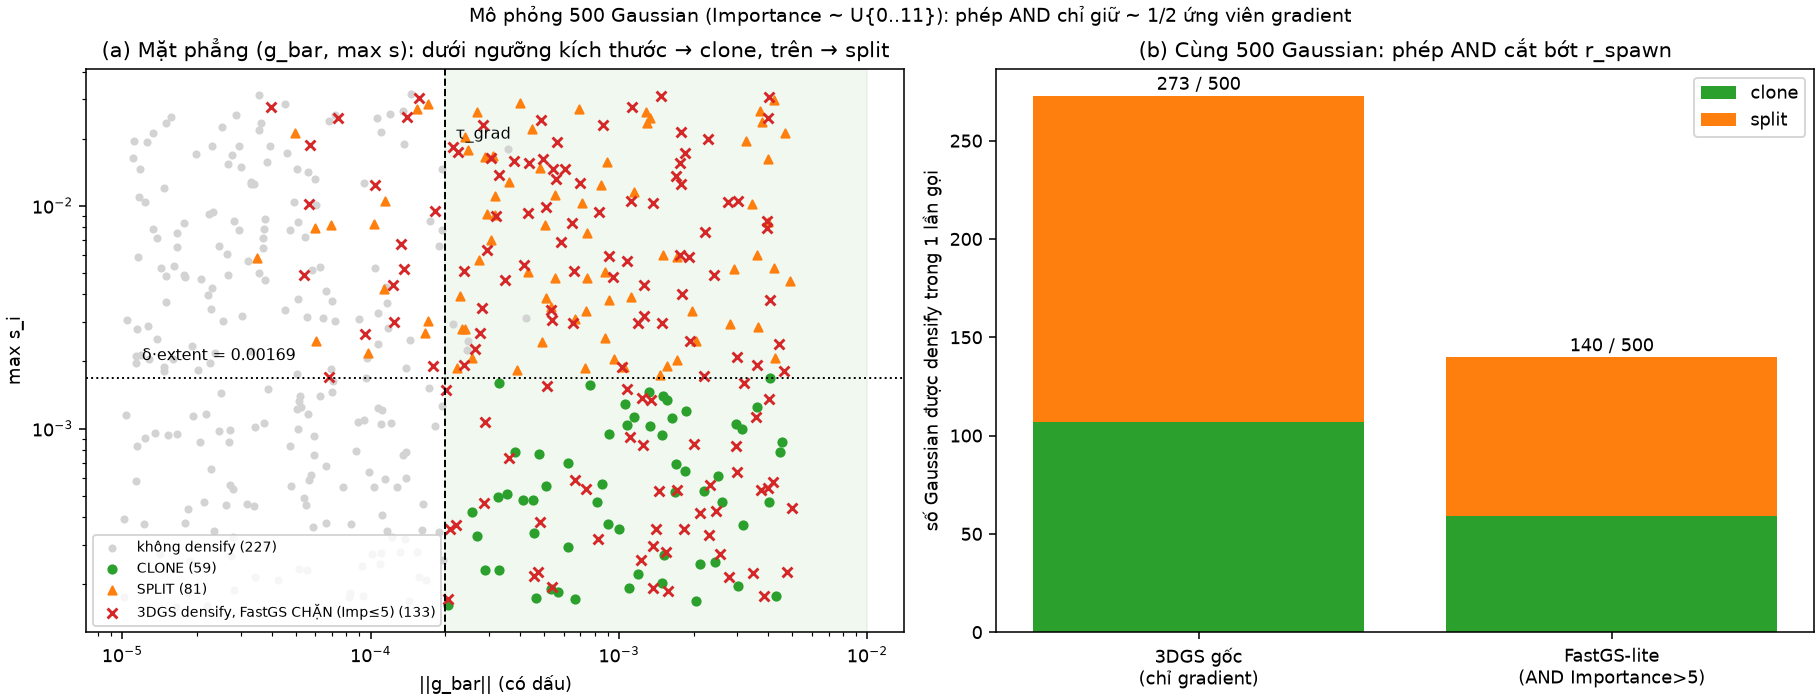
\includegraphics[width=0.95\linewidth]{4_4_clone-region-500.png}
\captionof{figure}{\footnotesize Mặt phẳng $(\bar g, \max s)$: phép AND cắt bớt số Gaussian được densify so với chỉ dùng gradient.}
\end{column}
\end{columns}
\end{frame}

% --- 4_5_scene-extent.png ---
\begin{frame}{Scene Extent: chuẩn hoá ngưỡng kích thước theo camera}
\begin{columns}[T]
\begin{column}{0.5\linewidth}
\footnotesize
\begin{itemize}
  \item \texttt{getNerfppNorm}: tâm camera trung bình $\bar c = \frac{1}{V}\sum_v c_v$, bán kính lớn nhất $\text{diag} = \max_v \|c_v - \bar c\|$, và
  \[
    \text{extent} = 1.1 \times \text{diag}
  \]
  \item Cảnh đồ chơi (3 camera): $c_1=(0,0,-4)$, $c_2=(1.5,0,-4)$, $c_3=(-1.5,0.5,-4)$ $\Rightarrow \bar c \approx (0, 0.1667, -4)$, $\text{diag} \approx 1.5366$, $\text{extent} \approx 1.6903$.
  \item Extent chỉ phụ thuộc \textbf{vị trí camera}, không phụ thuộc điểm SfM hay vị trí Gaussian.
  \item Ba mức kích thước tham chiếu: $\delta\cdot\text{extent} = 0.00169$ (ngưỡng clone/split), $0.1\cdot\text{extent} \approx 0.169$ (ngưỡng prune "quá to"), và $\min/\max s_i$ thực tế của 4 Gaussian $\in [0.8505, 1.1150]$.
  \item Vì $0.00169 \ll 0.85\text{--}1.12$, cả 4 Gaussian của cảnh đồ chơi rơi vào nhánh split trong ví dụ này.
\end{itemize}
\end{column}
\begin{column}{0.48\linewidth}
\centering
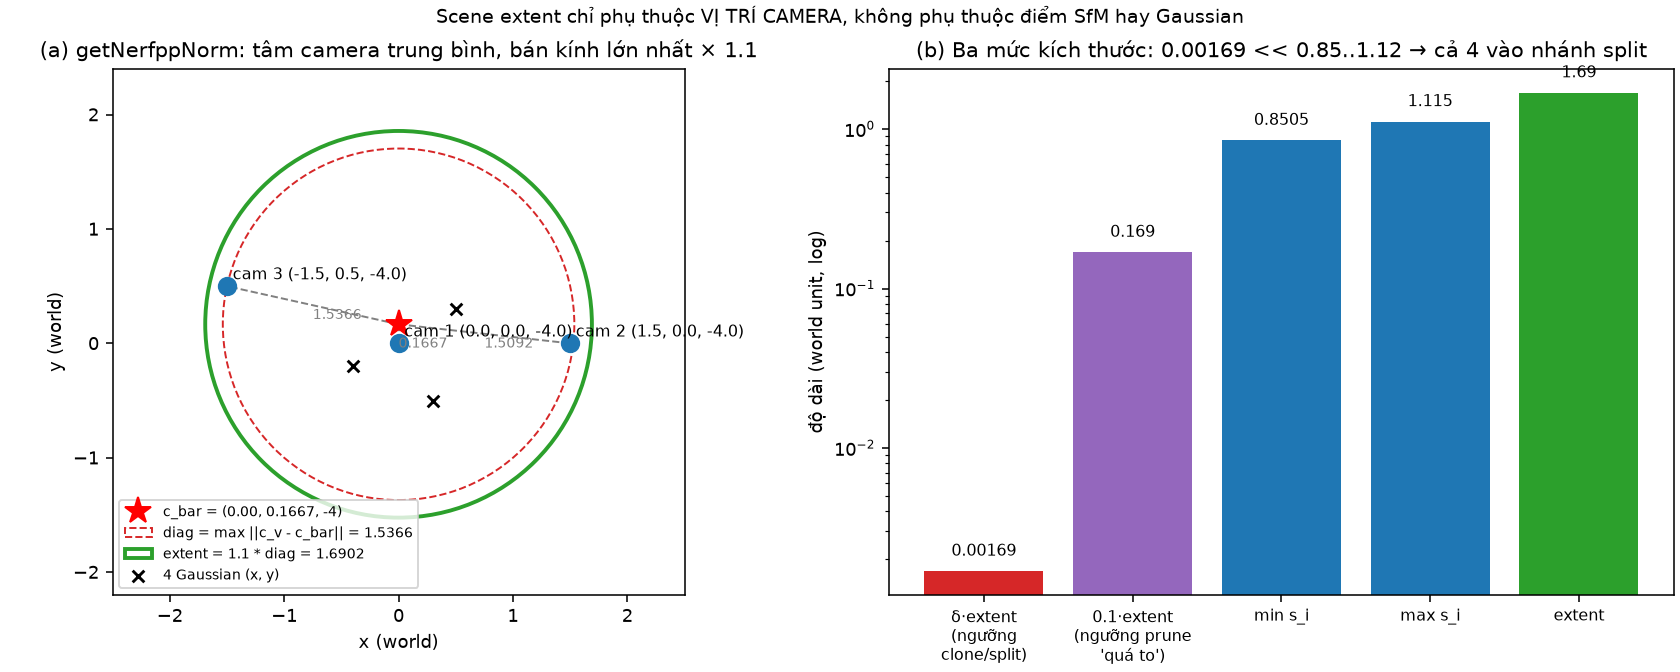
\includegraphics[width=0.95\linewidth]{4_5_scene-extent.png}
\captionof{figure}{\footnotesize Scene extent = $1.1 \times$ khoảng cách xa nhất từ camera đến tâm trung bình.}
\end{column}
\end{columns}
\end{frame}

% --- 4_6_decision-diagram.png ---
\begin{frame}{Sơ đồ quyết định densify đầy đủ}
\begin{columns}[T]
\begin{column}{0.48\linewidth}
\footnotesize
\begin{itemize}
  \item Áp dụng cho mỗi Gaussian $i$, mỗi 100 (hoặc 500) vòng lặp, khi $500 < t < 15000$.
  \item \textbf{Bước 1 — kích thước chọn nhánh:}
  \[
    \max s_i \le \delta \cdot \text{extent} \;?
  \]
  \item \textbf{Nhánh NHỎ (under-reconstruction):} nếu $\bar g_i \ge \tau_{\text{grad}} = 2\times10^{-4}$ \textbf{và} $\text{Imp}_i > 5$ $\Rightarrow$ \textbf{CLONE} ($\theta_{\text{new}} = \theta_i$, $1 \to 2$, giữ bản gốc).
  \item \textbf{Nhánh TO (over-reconstruction):} nếu $\bar g_{\text{abs},i} \ge \tau_{\text{abs}} = 1.2\times10^{-3}$ \textbf{và} $\text{Imp}_i > 5$ $\Rightarrow$ \textbf{SPLIT} (2 con, $\mu + R\cdot\varepsilon$, $s/1.6$, xoá gốc, $1 \to 2$).
  \item Nếu điều kiện Importance không thoả: 3DGS gốc vẫn densify (chỉ cần gradient đạt), FastGS-lite thì không.
  \item Nguồn: \texttt{densify\_and\_prune\_fastgs}, \texttt{gaussian\_model.py:449-462}.
\end{itemize}
\end{column}
\begin{column}{0.5\linewidth}
\centering
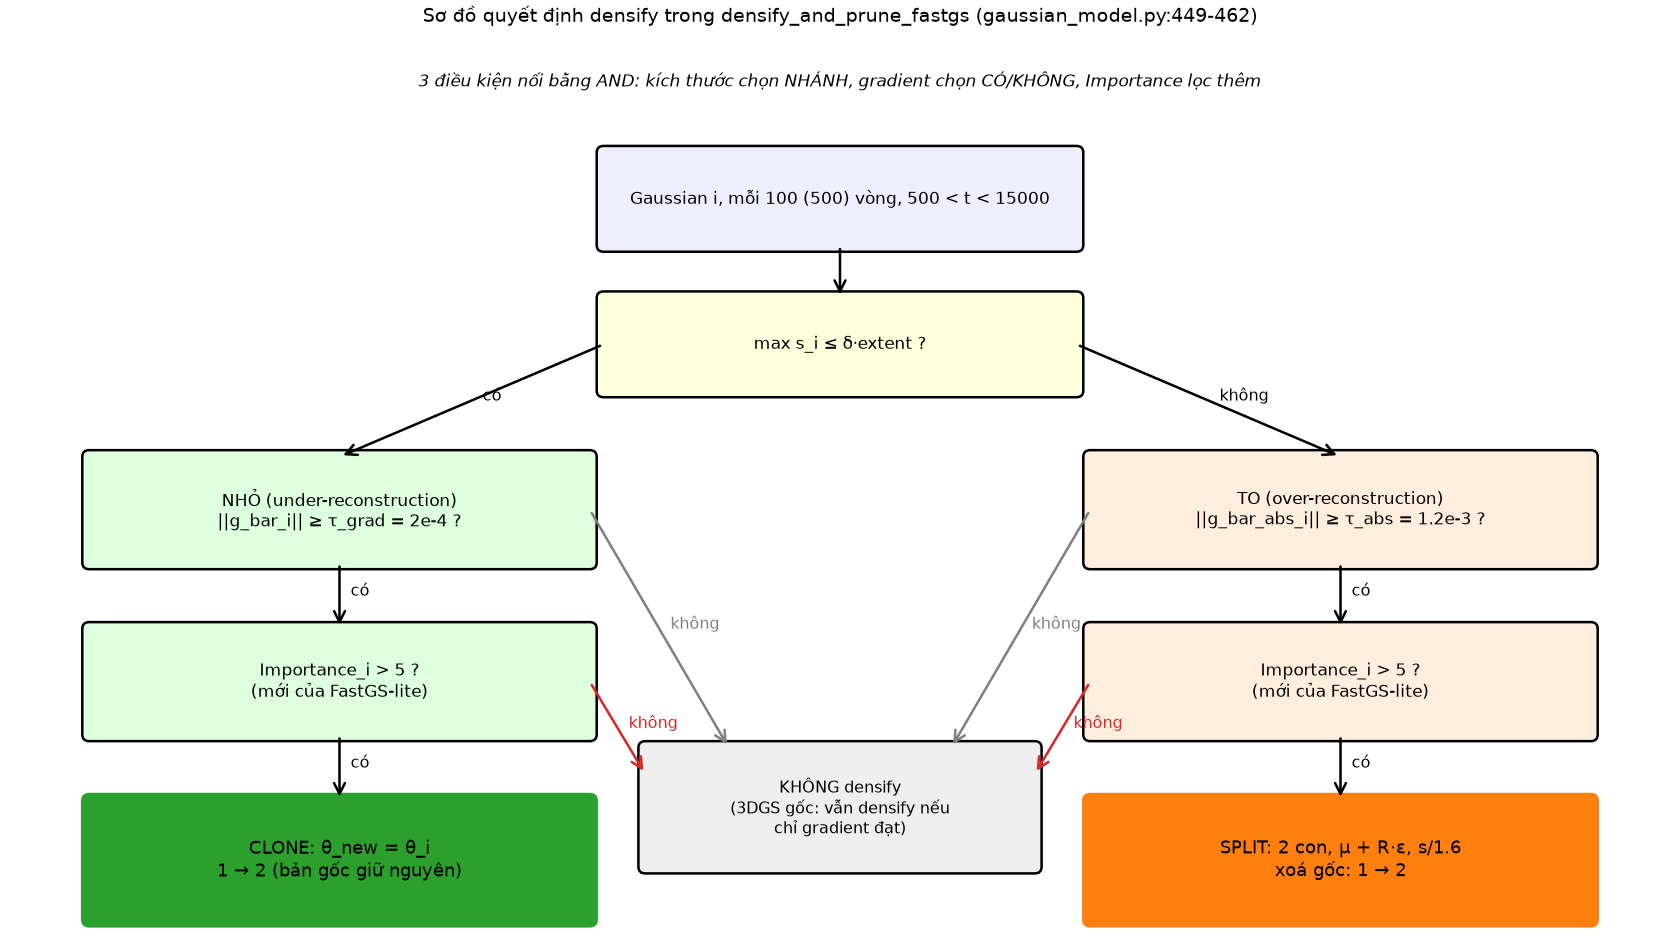
\includegraphics[width=\linewidth]{4_6_decision-diagram.png}
\captionof{figure}{\footnotesize 3 điều kiện nối bằng AND: kích thước chọn nhánh, gradient chọn có/không, Importance lọc thêm.}
\end{column}
\end{columns}
\end{frame}

% --- 4_7_under-vs-over.png ---
\begin{frame}{Under- vs. Over-reconstruction}
\begin{columns}[T]
\begin{column}{0.5\linewidth}
\footnotesize
\begin{itemize}
  \item Cùng một tín hiệu "gradient vị trí lớn" nhưng là hai bệnh khác nhau, phân biệt bằng \textbf{kích thước} Gaussian.
  \item \textbf{Under-reconstruction:} vùng cần phủ (GT) rộng ($s = 1.4$) nhưng 1 Gaussian quá nhỏ ($s = 0.45$) chưa phủ hết $\Rightarrow$ gradient kéo nó giãn ra $\Rightarrow$ \textbf{CLONE} thêm bản để phủ; sau tối ưu: 2 bản tách ra ở $\pm 0.55$.
  \item \textbf{Over-reconstruction:} 2 chi tiết nhỏ, hẹp ($s = 0.3$, tại $x = -0.8$ và $x = 0.8$) nhưng 1 Gaussian quá to ($s = 1.2$) che lấp cả hai $\Rightarrow$ gradient hai nửa ngược chiều nhau (giá trị \texttt{abs} lớn dù tổng có dấu nhỏ) $\Rightarrow$ \textbf{SPLIT} thành 2 con nhỏ hơn khớp đúng 2 chi tiết.
  \item Đây chính là lý do sơ đồ quyết định (Slide trước) dùng kích thước để chọn nhánh clone/split, còn gradient (có dấu / trị tuyệt đối) để xác nhận có densify hay không.
\end{itemize}
\end{column}
\begin{column}{0.48\linewidth}
\centering
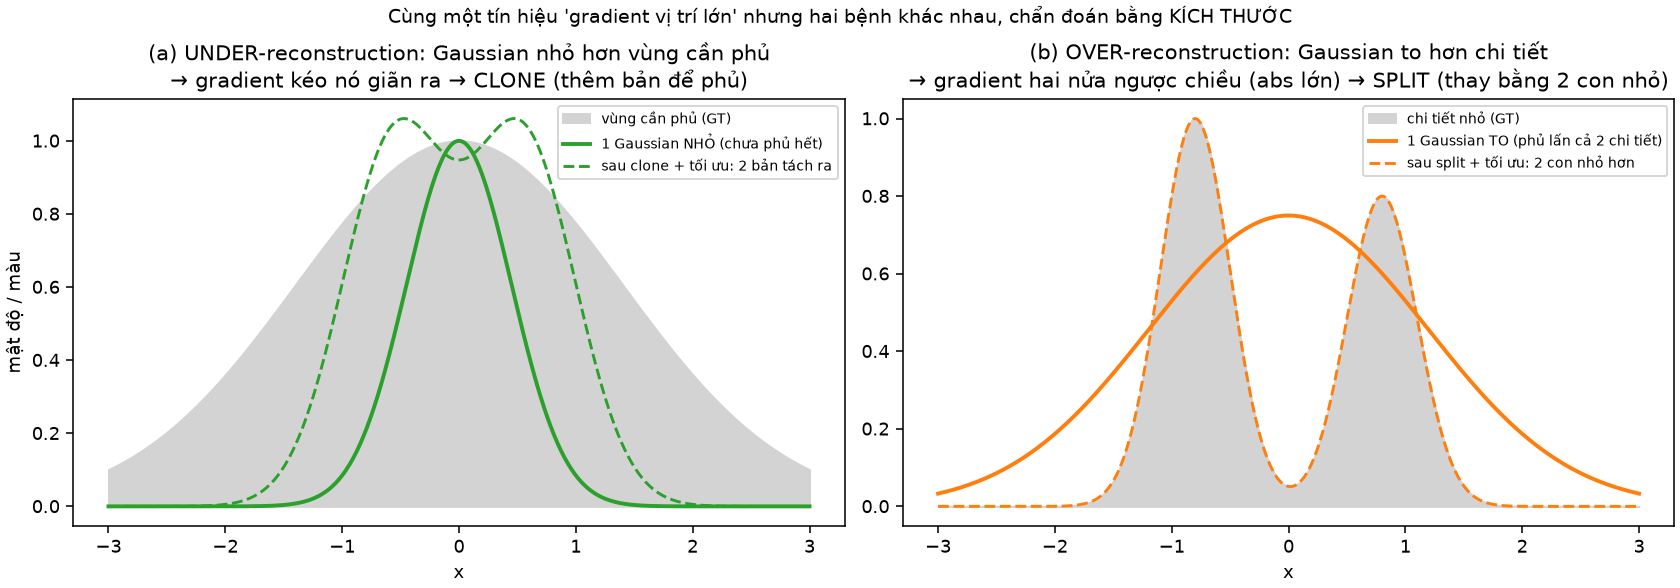
\includegraphics[width=0.95\linewidth]{4_7_under-vs-over.png}
\captionof{figure}{\footnotesize (a) Gaussian nhỏ hơn vùng cần phủ $\to$ clone. (b) Gaussian to hơn chi tiết $\to$ split.}
\end{column}
\end{columns}
\end{frame}

% --- 4_8_split-geometry.png ---
\begin{frame}{Hình học phép Split: sinh 2 Gaussian con}
\begin{columns}[T]
\begin{column}{0.52\linewidth}
\footnotesize
\begin{itemize}
    \item Gaussian gốc $(\mu, \Sigma)$ với $\Sigma = R(q)\,\mathrm{diag}(s)^2\,R(q)^\top$ bị \textbf{xoá} sau split ($1 \to 2$).
    \item Vị trí 2 con lấy mẫu quanh $\mu$ theo chính hình dạng gốc:
    \[
        \mu_{\text{con}} = \mu + R(q)\cdot \varepsilon, \qquad \varepsilon \sim \mathcal{N}(0, \mathrm{diag}(s)^2)
    \]
    \item Scale con giảm theo hệ số cố định trong code (\texttt{scale / (0.8 * N)} với $N{=}2$ con), tức $s_{\text{con}} = s / 1.6$.
    \item Rotation $R(q)$ giữ \textbf{nguyên} cho cả 2 con — chỉ tâm và scale thay đổi, hướng ellipsoid không đổi.
    \item Hệ quả: 2 ellipsoid con nhỏ hơn ($s/1.6$), lệch tâm ngẫu nhiên nhưng cùng hướng với ellipsoid cha.
\end{itemize}
\end{column}
\begin{column}{0.48\linewidth}
\centering
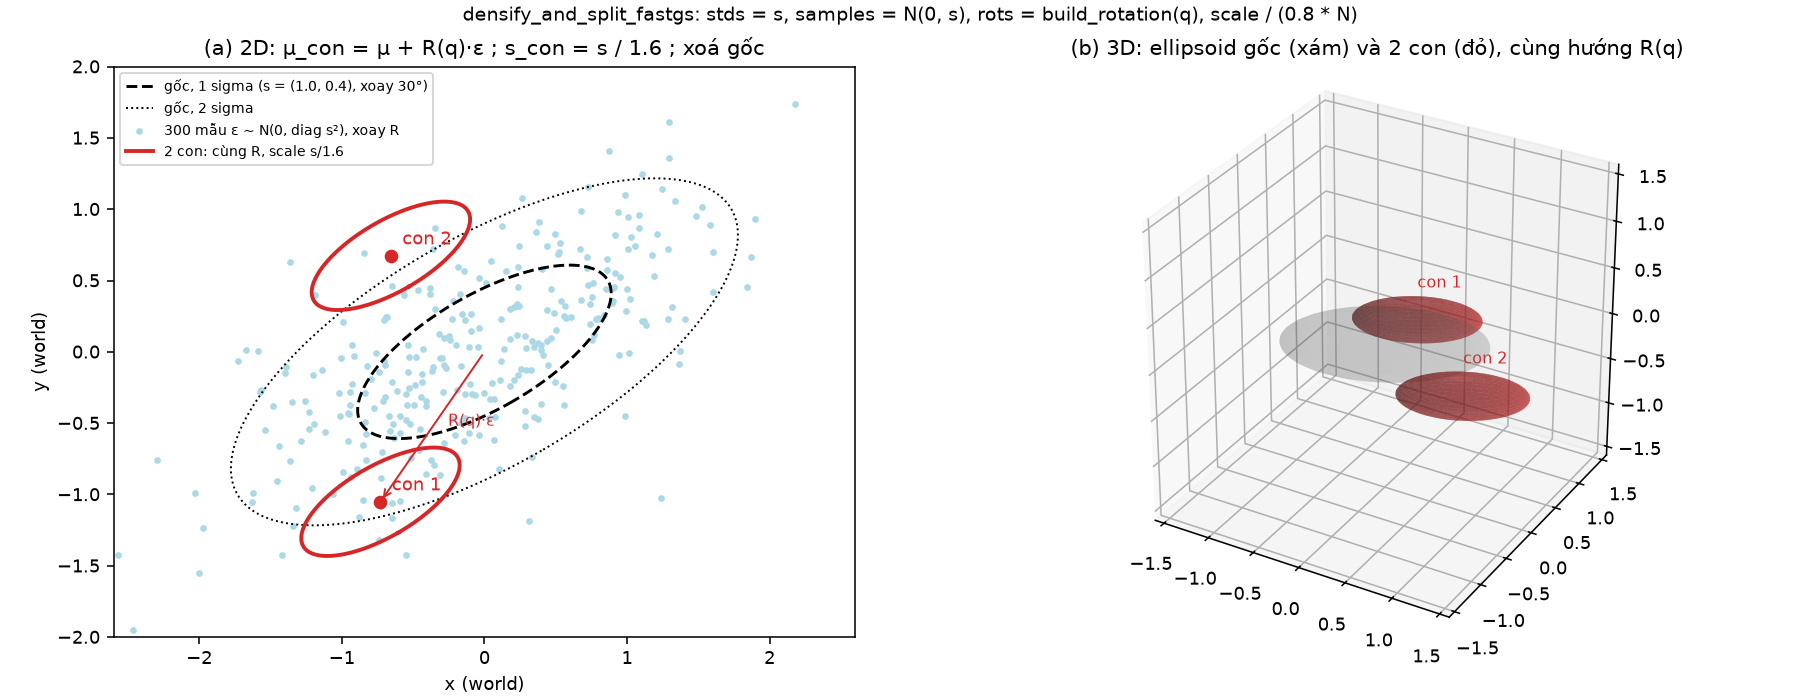
\includegraphics[width=0.95\linewidth]{4_8_split-geometry.png}
\captionof{figure}{\footnotesize (a) 2D: ellipse gốc (nét đứt) và 2 ellipse con (đỏ), $\mu_{\text{con}}=\mu+R(q)\varepsilon$, $s_{\text{con}}=s/1.6$. (b) 3D: ellipsoid gốc (xám) và 2 con (đỏ) cùng hướng $R(q)$.}
\end{column}
\end{columns}
\end{frame}

% --- 4_9_split-distribution.png ---
\begin{frame}{Phân bố lấy mẫu vị trí con và hệ số chia $1.6$}
\begin{columns}[T]
\begin{column}{0.52\linewidth}
\footnotesize
\begin{itemize}
    \item Với nhiều lần split cùng một Gaussian, tâm con phân bố quanh gốc theo đúng elip đẳng mật độ của $\Sigma$ gốc (do $\varepsilon \sim \mathcal{N}(0, \mathrm{diag}(s)^2)$ rồi xoay bởi $R(q)$).
    \item So sánh ước số chia scale: $s/1$ (2 con chồng lấn gần như trùng gốc), $s/1.6$ (giá trị dùng trong code — vẫn phủ được vùng gốc nhưng đã tách biệt), $s/2$, $s/3$ (2 con tách rời, để hở vùng giữa).
    \item Hệ số $0.8$ trong công thức \texttt{scale/(0.8*N)} với $N{=}2$ được chọn sao cho tổng "khối lượng" phủ của 2 con xấp xỉ khối lượng gốc, tránh để hở hoặc chồng lấn quá mức.
    \item Minh hoạ trên cảnh đồ chơi (seed 0): 4 Gaussian gốc $\to$ 8 Gaussian con, bán kính con $= s/1.6 \approx 0.53\text{–}0.70$ (world unit), do $s$ gốc $\in \{0.85,\,0.94,\,1.12,\,0.89\}$.
    \item Vì rotation $R(q)$ ở cảnh đồ chơi bằng $I$, $\varepsilon$ cộng thẳng vào $\mu$ không cần xoay.
\end{itemize}
\end{column}
\begin{column}{0.48\linewidth}
\centering
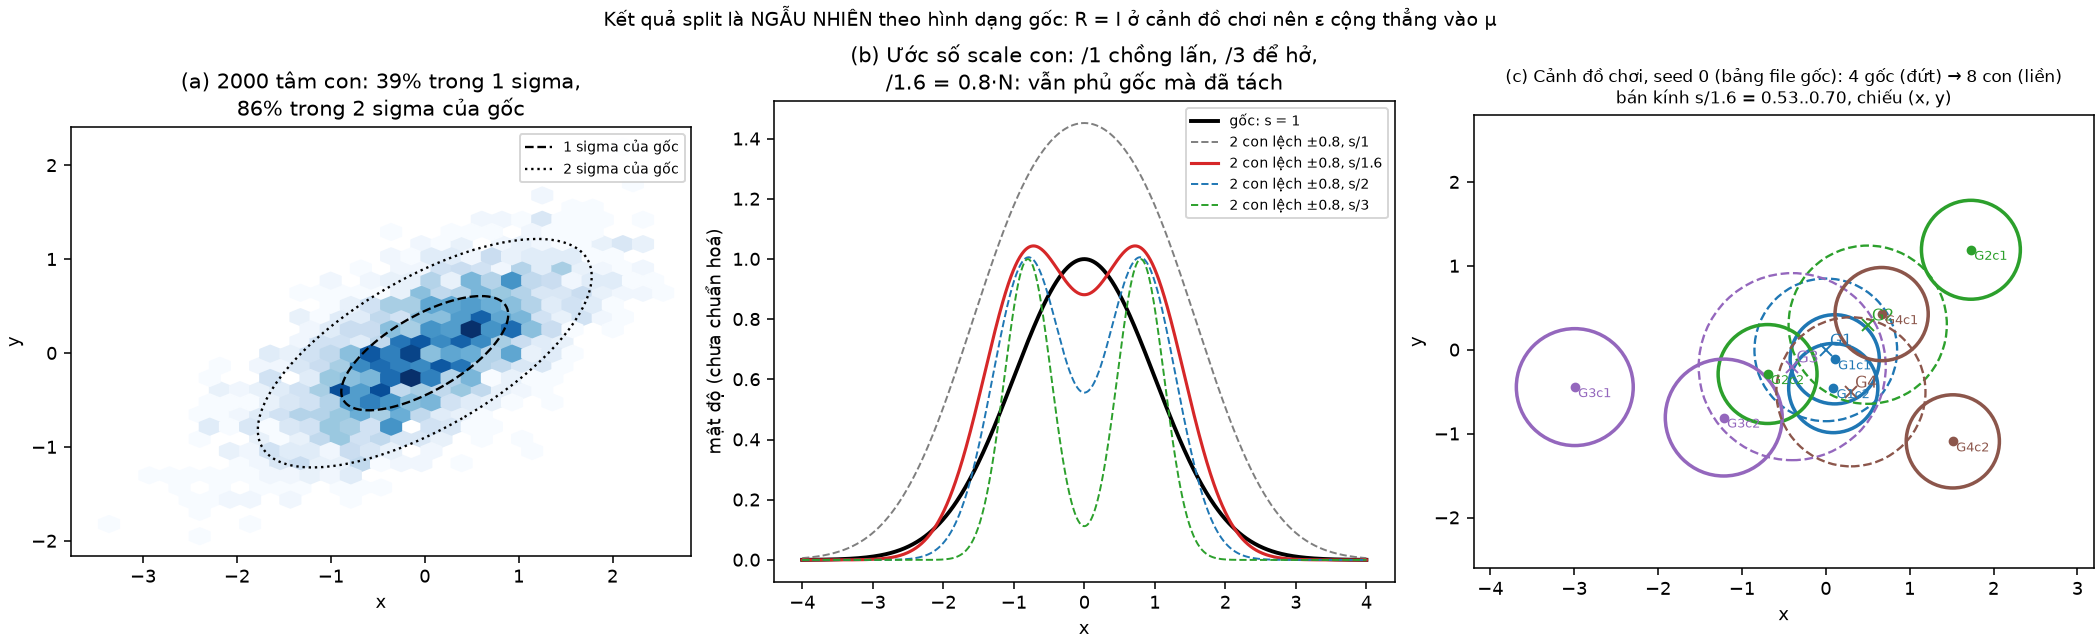
\includegraphics[width=0.95\linewidth]{4_9_split-distribution.png}
\captionof{figure}{\footnotesize (a) Histogram tâm con quanh gốc theo elip $\Sigma$. (b) Mật độ 1D: gốc $s{=}1$ so với tổng 2 con ở các ước số $1/1.6/2/3$. (c) Cảnh đồ chơi: 4 gốc (đứt) $\to$ 8 con (liền), $s/1.6$.}
\end{column}
\end{columns}
\end{frame}

% --- 4_10_clone-symmetry-break.png ---
\begin{frame}{Clone: phá vỡ đối xứng nhờ trạng thái Adam}
\begin{columns}[T]
\begin{column}{0.52\linewidth}
\footnotesize
\begin{itemize}
    \item Khi \textbf{CLONE} (không phải split), 2 bản sao được tạo với \textbf{cùng} tham số: $\theta_{\text{new}} = \theta_i$ — vị trí, scale, rotation, opacity, SH đều trùng khớp tại $t{=}0$.
    \item Nếu không có cơ chế phá đối xứng nào, 2 bản nhận gradient \textbf{giống hệt nhau} ở mọi bước và không bao giờ tách biệt.
    \item Cơ chế phá đối xứng thực tế không phải dịch chuyển vị trí, mà đến từ \texttt{cat\_tensors\_to\_optimizer}: bản clone mới có \texttt{exp\_avg}, \texttt{exp\_avg\_sq} (Adam $m, v$) khởi tạo lại bằng $0$, trong khi bản gốc đã mang lịch sử Adam tích luỹ từ trước.
    \item Vì bộ đếm bước \texttt{step} dùng chung cho cả nhóm ($t = t_{\text{gốc}} + k$), bias-correction $\hat m = m/(1-\beta_1^t)$ áp dụng \textbf{không đối xứng} lên 2 bản có $m, v$ khác nhau $\to$ 2 quỹ đạo cập nhật lệch nhau ngay từ bước đầu.
    \item Kết quả: $|\mu_{\text{gốc}} - \mu_{\text{clone}}|$ tăng dần theo bước tối ưu dù gradient ban đầu bằng nhau.
\end{itemize}
\end{column}
\begin{column}{0.48\linewidth}
\centering
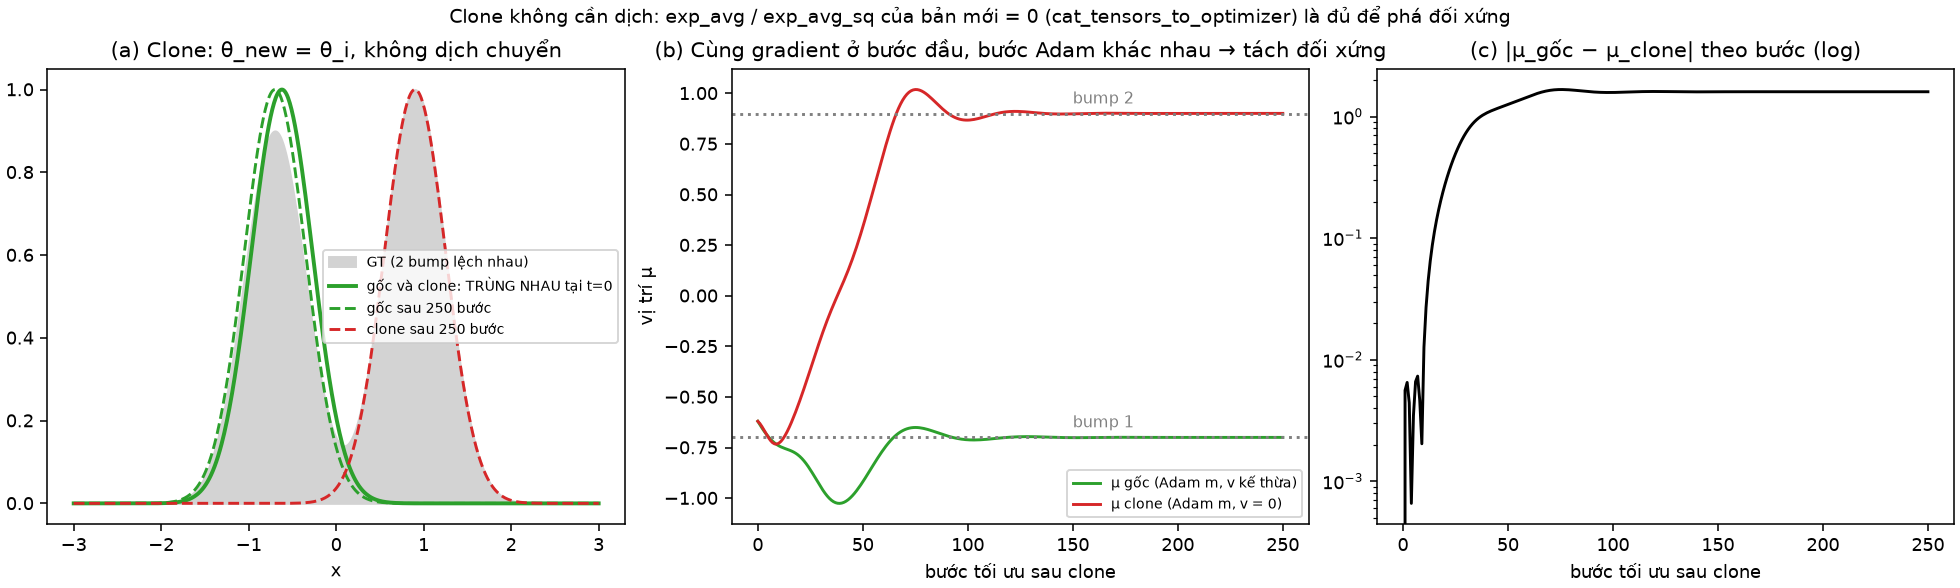
\includegraphics[width=0.95\linewidth]{4_10_clone-symmetry-break.png}
\captionof{figure}{\footnotesize (a) Gốc và clone trùng nhau tại $t{=}0$, tách dần sau $T$ bước. (b) Quỹ đạo $\mu$: gốc kế thừa $(m,v)$, clone khởi tạo $(0,0)$. (c) $|\mu_{\text{gốc}}-\mu_{\text{clone}}|$ tăng theo bước (log).}
\end{column}
\end{columns}
\end{frame}

% --- 4_11_n-growth.png ---
\begin{frame}{Tăng trưởng $N$ qua các vòng Densify}
\begin{columns}[T]
\begin{column}{0.52\linewidth}
\footnotesize
\begin{itemize}
    \item Sau mỗi vòng densify, số Gaussian biến đổi theo:
    \[
        N_{k+1} = N_k\,(1 + r_{\text{spawn}})\,(1 - r_{\text{prune}}), \qquad q = (1+r_{\text{spawn}})(1-r_{\text{prune}})
    \]
    với $r_{\text{spawn}} = f_{\text{clone}} + f_{\text{split}}$ là tỉ lệ Gaussian được nhân bản mỗi vòng.
    \item Sau $n$ vòng: $N_n = N_0 \cdot q^n$ — tăng trưởng theo \textbf{luỹ thừa}, không tuyến tính.
    \item Cửa sổ densify chạy từ iteration $500$ đến $15000$ (\texttt{densify\_from\_iter}, \texttt{densify\_until\_iter}); với \texttt{densification\_interval}$=100$: $n=144$ vòng; với interval$=500$: $n=28$ vòng.
    \item Ví dụ $r_{\text{spawn}}{=}0.15$, $r_{\text{prune}}{=}0.05 \Rightarrow q{=}1.0925$: sau $n{=}28$ vòng $q^{28}\approx 1.0925^{28}$; sau $n{=}144$ vòng $q^{144}\approx 1.0925^{144}$ (chênh lệch nhiều bậc độ lớn).
    \item Tốc độ tăng $N$ giảm dần về cuối do $r_{\text{spawn}}$ tự nhiên thu hẹp khi scene đã đủ dày đặc (ít Gaussian còn thoả điều kiện gradient/Importance).
\end{itemize}
\end{column}
\begin{column}{0.48\linewidth}
\centering
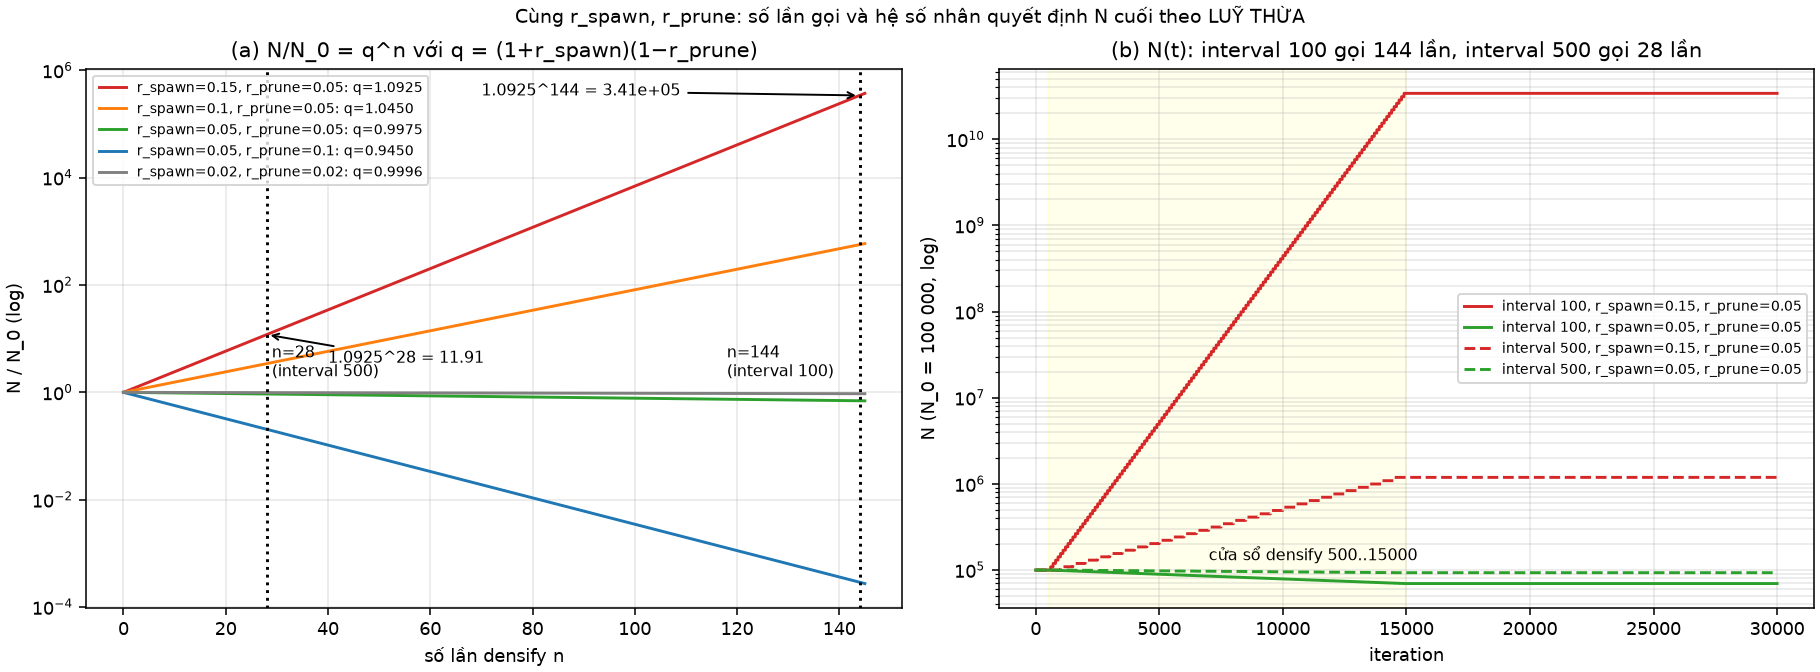
\includegraphics[width=0.95\linewidth]{4_11_n-growth.png}
\captionof{figure}{\footnotesize (a) $N/N_0 = q^n$ theo số vòng $n$, nhiều cặp $(r_{\text{spawn}}, r_{\text{prune}})$. (b) $N(t)$ theo iteration: interval $100$ (144 vòng) so với interval $500$ (28 vòng).}
\end{column}
\end{columns}
\end{frame}

% --- 4_12_stats-reset.png ---
\begin{frame}{Reset thống kê tích luỹ sau mỗi vòng Densify}
\begin{columns}[T]
\begin{column}{0.52\linewidth}
\footnotesize
\begin{itemize}
    \item Trong một chu kỳ densify (mỗi \texttt{densification\_interval} $=100$ vòng), 3 tensor tích luỹ theo Gaussian:
    \begin{itemize}
        \footnotesize
        \item \texttt{xyz\_gradient\_accum} — tổng $\|g\|$ khi hữu hình.
        \item \texttt{denom} — số lần hữu hình (radii $>0$).
        \item \texttt{max\_radii2D} — bán kính chiếu 2D lớn nhất từng đạt.
    \end{itemize}
    \item Ngay sau lệnh \texttt{densify\_and\_prune\_fastgs}, hàm \texttt{densification\_postfix} đưa \textbf{cả 3 tensor về 0} cho \textbf{toàn bộ} $N$ (kể cả các Gaussian \textbf{không} được clone/split ở vòng đó).
    \item Ngưỡng \texttt{max\_screen\_size}$=20$ px chỉ được bật kiểm tra khi $t > 3000$ — dùng \texttt{max\_radii2D} để prune Gaussian chiếm màn hình quá lớn.
    \item Nếu quên reset: thống kê của vòng trước sẽ cộng dồn sai vào vòng sau, khiến \texttt{g\_bar = accum/denom} bị lệch và quyết định densify/prune sai tín hiệu.
\end{itemize}
\end{column}
\begin{column}{0.48\linewidth}
\centering
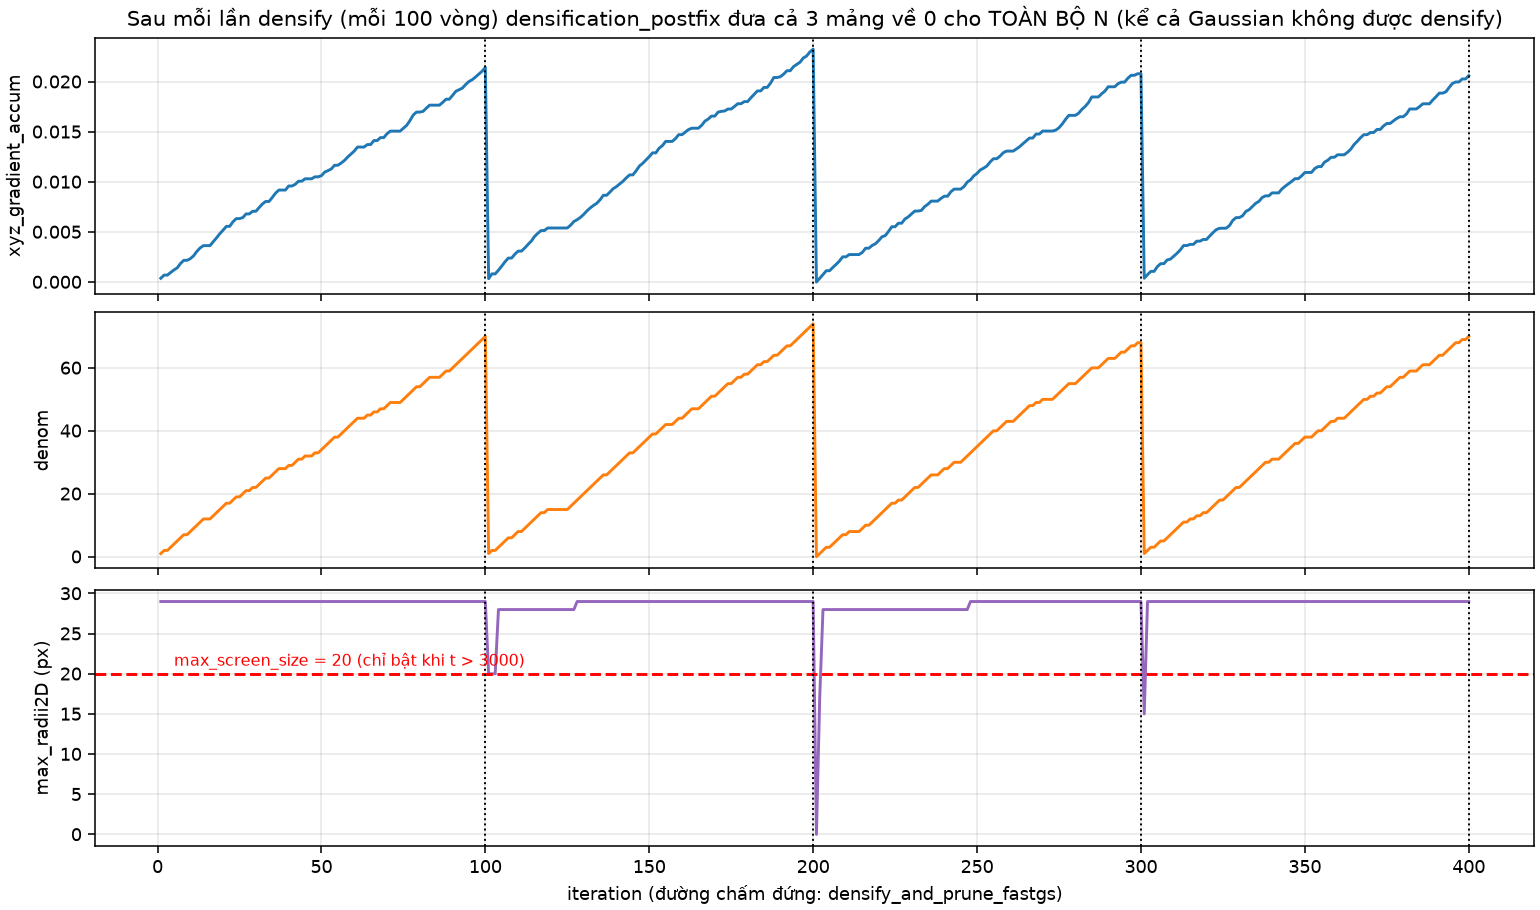
\includegraphics[width=0.95\linewidth]{4_12_stats-reset.png}
\captionof{figure}{\footnotesize \texttt{xyz\_gradient\_accum}, \texttt{denom}, \texttt{max\_radii2D} theo iteration — mỗi vạch đứng (mỗi 100 vòng) là một lần \texttt{densification\_postfix} đưa cả 3 tensor về 0.}
\end{column}
\end{columns}
\end{frame}

% --- 4_13_index-layout.png ---
\begin{frame}{Bố trí lại Index/Tensor tham số sau Densify}
\begin{columns}[T]
\begin{column}{0.52\linewidth}
\footnotesize
\begin{itemize}
    \item Sau split, tensor tham số (position, scale, rotation, opacity, SH) được nối theo thứ tự cố định:
    \[
        \texttt{cat(gốc, con)} \;\to\; [G_1..G_N,\ G_1c_1..G_Nc_1,\ G_1c_2..G_Nc_2]
    \]
    tức mẫu \texttt{repeat(N,1)} — mỗi Gaussian gốc sinh 2 con nằm cách nhau $N$ vị trí trong tensor.
    \item \texttt{prune\_filter = cat(mask\_gốc, zeros(N·sum))} xoá toàn bộ Gaussian gốc đã split, chỉ giữ 2 lớp con.
    \item Optimizer state (\texttt{exp\_avg}, \texttt{exp\_avg\_sq}) và 3 tensor thống kê (accum, denom, max\_radii2D) được nối/cắt \textbf{đồng bộ} theo cùng chỉ số, rồi reset về $0$ cho $N$ mới — không làm đứt gradient graph vì thao tác trên \texttt{.data}, ngoài autograd.
    \item Hệ quả phụ: \texttt{padded\_importance[:N]} (trọng số prune $1/(10^{-6}+1-\text{Pruning})$) chỉ áp cho 4 con đầu (lớp $c_1$) theo \textbf{chỉ số cũ}, không theo danh tính — 4 con lớp $c_2$ nhận trọng số $0$, miễn nhiễm prune ở vòng đó.
    \item Thứ tự thao tác trong \texttt{densify\_and\_prune\_fastgs}: (1) tính $\bar g,\bar g_{\text{abs}}$, \texttt{tmp\_radii=radii} (2) clone (3) split (4) \texttt{prune\_mask} + multinomial (5) opacity $\leftarrow \min(\alpha, 0.8)$ (6) \texttt{tmp\_radii=None}.
\end{itemize}
\end{column}
\begin{column}{0.48\linewidth}
\centering
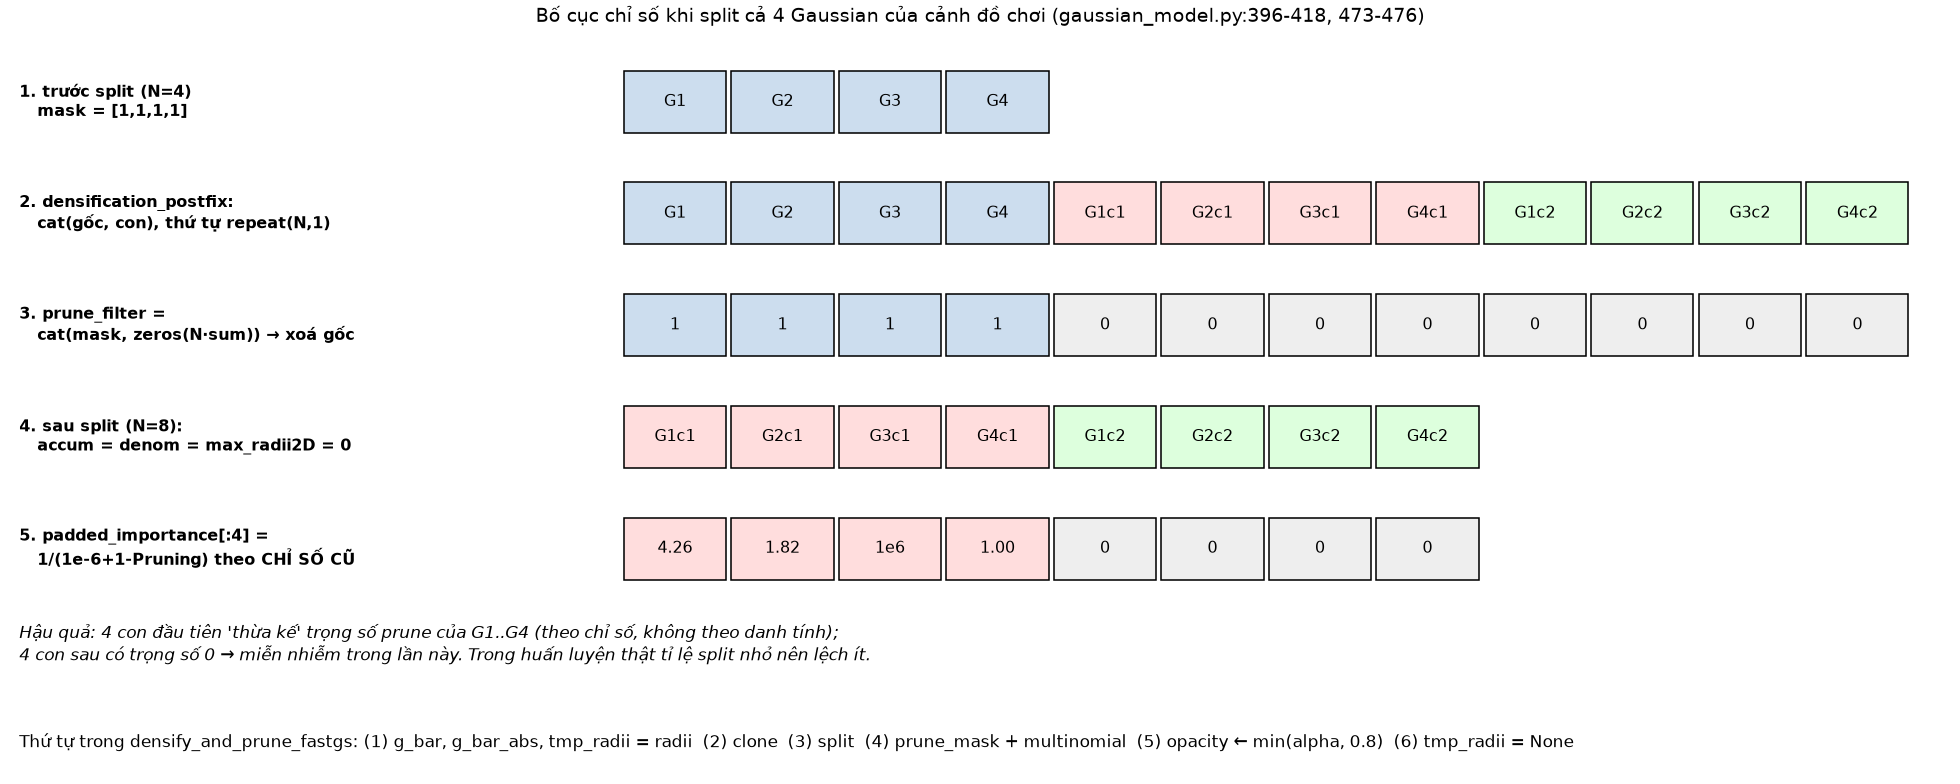
\includegraphics[width=0.95\linewidth]{4_13_index-layout.png}
\captionof{figure}{\footnotesize Bố cục chỉ số khi split 4 Gaussian: (1) trước split $N{=}4$ (2) \texttt{cat} gốc+con theo \texttt{repeat(N,1)} (3) \texttt{prune\_filter} xoá gốc (4) sau split $N{=}8$, thống kê reset $0$ (5) \texttt{padded\_importance} thừa kế theo chỉ số cũ.}
\end{column}
\end{columns}
\end{frame}


\section{ADC chuyên sâu — P5: Trọng số, Multinomial Resample \& Opacity Reset}
% --- 5_1_trong-so-N10.png ---
\begin{frame}{Từ điểm importance sang trọng số xoá: ví dụ $N=10$}
\begin{columns}[T]
\begin{column}{0.52\linewidth}
\footnotesize
\begin{itemize}
    \item Kịch bản giả định $N=10$ Gaussian với điểm Pruning\_i cho trước:
    \[
    P = [0{,}0.05,0{,}2,0{,}4,0{,}6,0{,}8,0{,}9,0{,}95,0{,}99,1{,}0]
    \]
    \item Tập ứng viên $C=\{3,6,8,9,10\}$ (chỉ số 1-based), ngân sách xoá
    \[
    \text{budget} = \lfloor 0{,}5\cdot |C| \rfloor = \lfloor 0{,}5 \cdot 5 \rfloor = 2
    \]
    \item Trọng số bị xoá tỉ lệ nghịch với $(1-P_i)$:
    \[
    w_i = \frac{1}{10^{-6} + (1-P_i)}
    \]
    \item Chuẩn hoá: $p_i = w_i / \sum_j w_j$.
    \item $w_i$ \textbf{phân kỳ} khi $P_i \to 1$: Gaussian số 10 ($P_{10}=1{,}0$) chiếm tới $99{,}99\%$ xác suất bị rút ở lượt đầu tiên -- gần như chắc chắn bị xoá.
\end{itemize}
\end{column}
\begin{column}{0.48\linewidth}
\centering
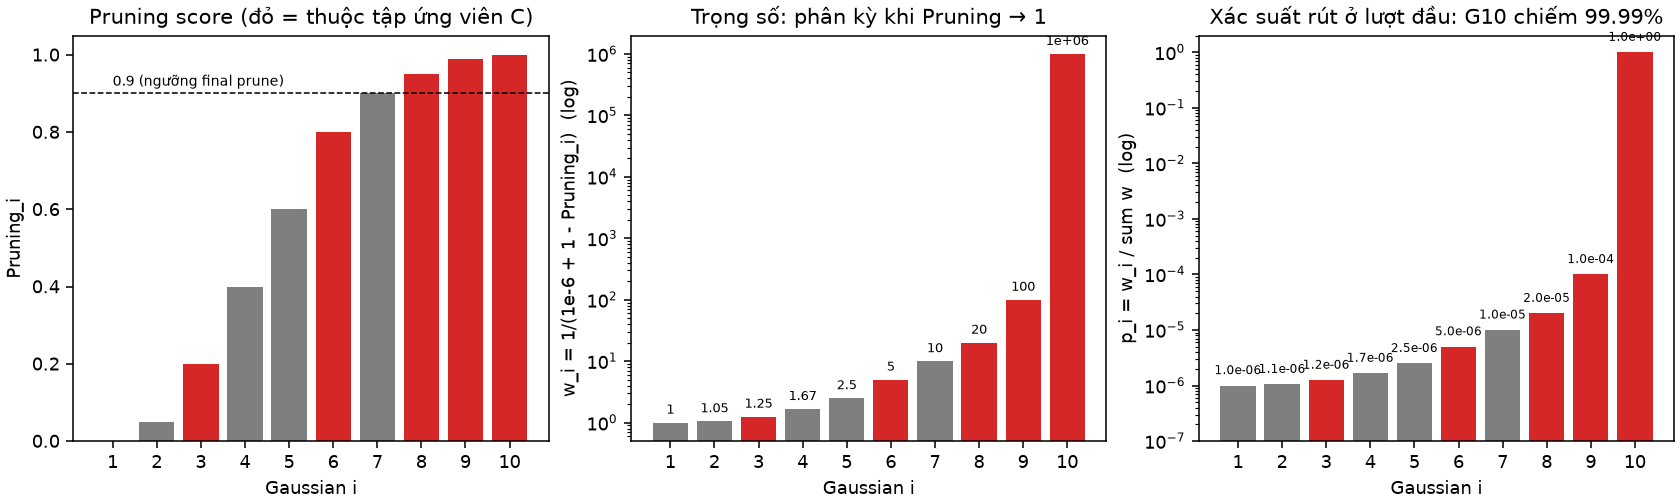
\includegraphics[width=0.98\linewidth]{5_1_trong-so-N10.png}
\captionof{figure}{\footnotesize $P_i$, trọng số $w_i$ (log) và xác suất $p_i$ (log) của 10 Gaussian; đỏ = thuộc tập ứng viên $C$.}
\end{column}
\end{columns}
\end{frame}

% --- 5_2_mo-phong-2000-lan.png ---
\begin{frame}{Kiểm chứng bằng mô phỏng: 2000 lần lấy mẫu multinomial}
\footnotesize
\begin{itemize}
    \item Lấy mẫu \texttt{multinomial\_no\_replacement}$(w,\text{budget}{=}2)$ lặp lại $T=2000$ lần (không hoàn lại, giống \texttt{torch.multinomial}).
    \item Xác suất lý thuyết $P(i \in S)$ với budget $=2$ tính chính xác bằng công thức bao gồm cả cặp:
    \[
    P(i \in S) = p_i + \sum_{j \neq i} p_j \cdot \frac{w_i}{W - w_j}, \qquad p_i = \frac{w_i}{W}, \; W=\sum_k w_k
    \]
    \item Tần suất thực nghiệm $i \in S$ qua 2000 lần khớp sát với $P(i\in S)$ lý thuyết -- xác nhận cơ chế lấy mẫu đúng như thiết kế.
    \item Tần suất \emph{thực sự bị xoá} = $S \cap C$: một Gaussian có thể được rút vào $S$ nhưng không thuộc $C$ nên không bị xoá (ví dụ G7 hay được rút nhưng không nằm trong tập ứng viên).
    \item Số Gaussian bị xoá thực tế trung bình $\approx$ giá trị hiển thị trên biểu đồ (thấp hơn budget=2 vì $S\cap C$ có thể nhỏ hơn $S$).
\end{itemize}
\centering
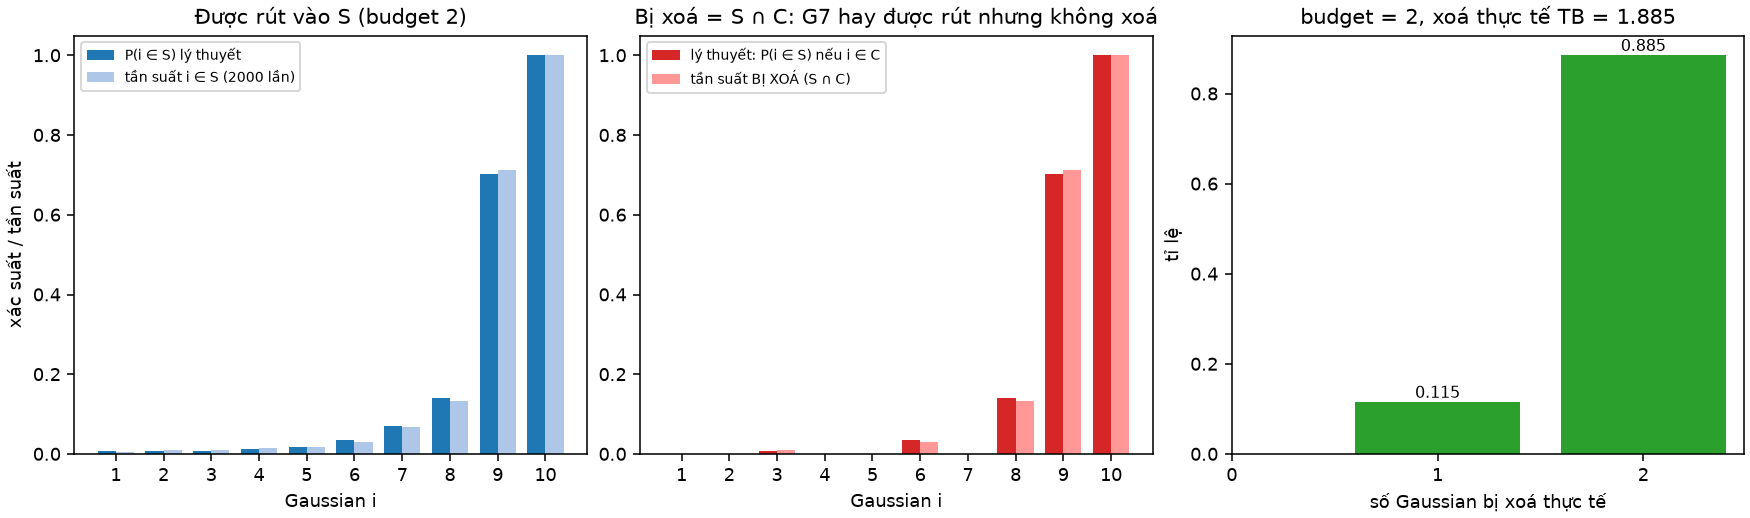
\includegraphics[width=0.62\linewidth]{5_2_mo-phong-2000-lan.png}
\captionof{figure}{\footnotesize Trái: $P(i\in S)$ lý thuyết vs tần suất thực nghiệm. Giữa: xác suất/tần suất bị xoá $S\cap C$. Phải: phân bố số Gaussian bị xoá thực tế mỗi lượt.}
\end{frame}

% --- 5_3_topk-vs-multinomial.png ---
\begin{frame}{Top-k cứng vs.\ Multinomial: hai chiến lược pruning}
\begin{columns}[T]
\begin{column}{0.5\linewidth}
\footnotesize
\begin{itemize}
    \item Mô phỏng $N=300$ Gaussian, điểm số $P_i$ chuẩn hoá min--max từ \texttt{Beta}$(2{,}2{,}5)$; tập ứng viên $C$ chọn ngẫu nhiên $40\%$ quần thể (độc lập với $P_i$), budget $=\lfloor 0{,}5|C|\rfloor$.
    \item \textbf{Top-k cứng (deterministic):} sắp xếp $C$ giảm dần theo $P_i$, xoá đúng \texttt{budget} phần tử điểm thấp nhất.
    \begin{itemize}
        \item[+] Dễ đoán, luôn xoá đúng số lượng.
        \item[--] Cắt sạch theo một ngưỡng cứng -- có thể xoá nhầm cả một cụm liền kề có điểm số tương tự nhau.
    \end{itemize}
    \item \textbf{Multinomial (stochastic):} rút mẫu không hoàn lại theo $w_i \propto 1/(10^{-6}+1-P_i)$ trên toàn $N$, giao với $C$.
    \begin{itemize}
        \item[+] Đa dạng hơn, tránh xoá đồng loạt một vùng.
        \item[--] Có nhiễu: số lượng xoá thực tế thường \emph{ít hơn} budget vì $S\cap C$ nhỏ hơn $S$.
    \end{itemize}
\end{itemize}
\end{column}
\begin{column}{0.5\linewidth}
\centering
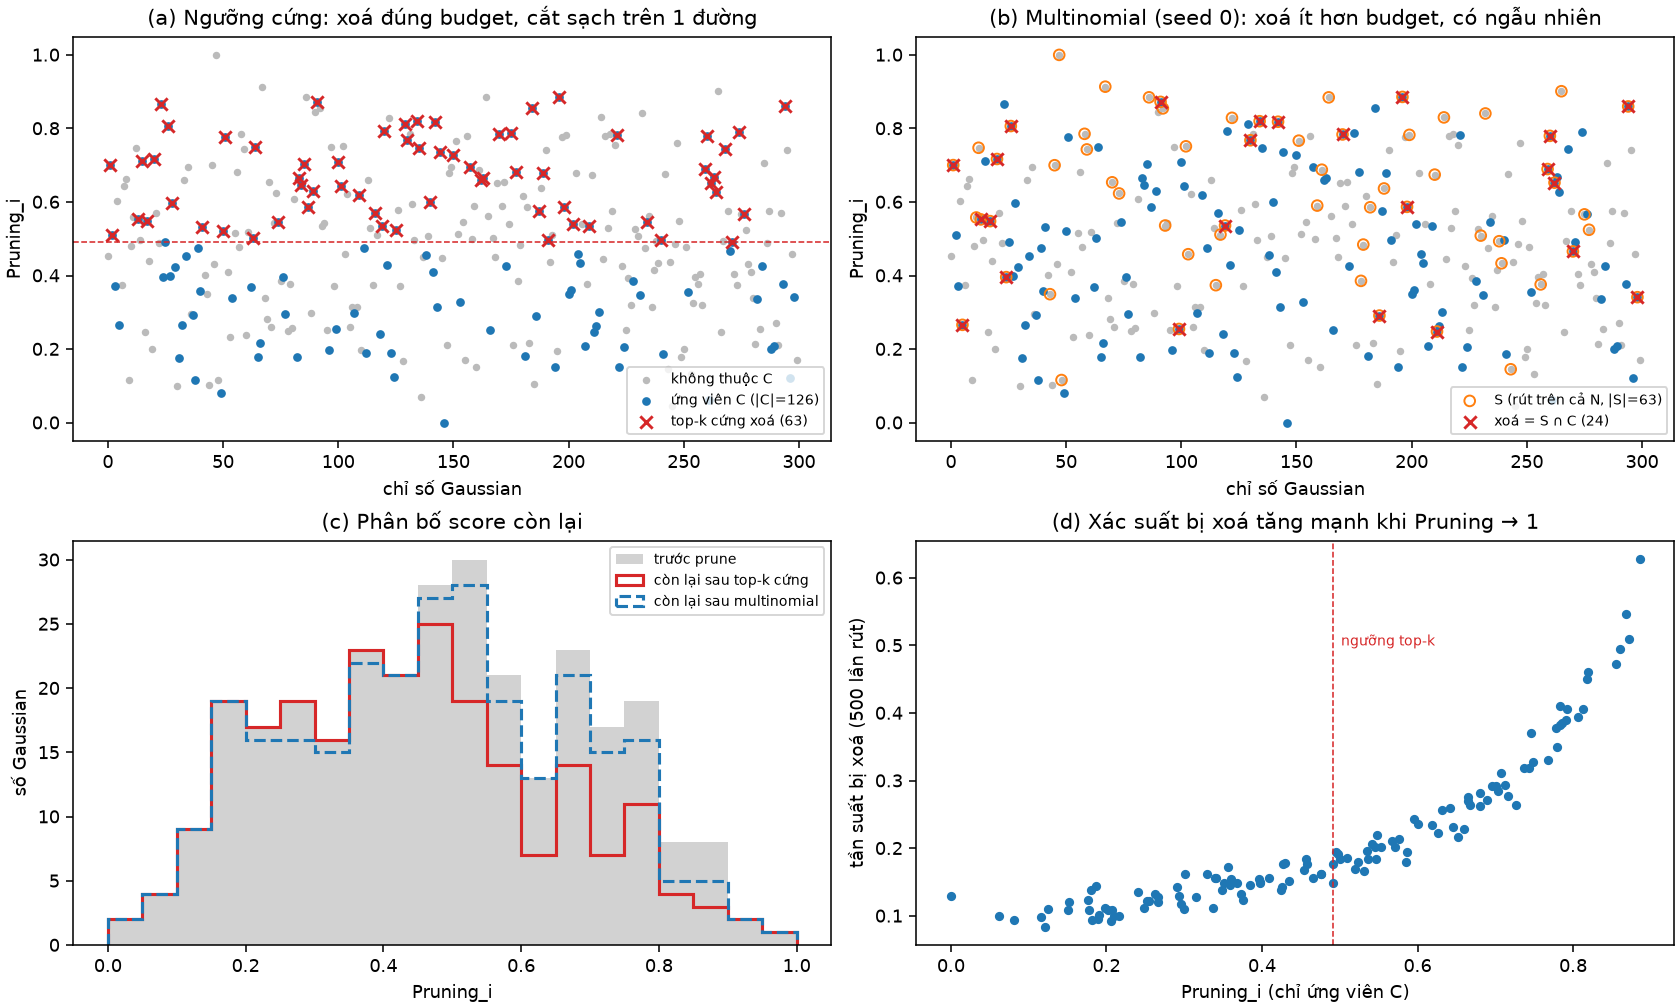
\includegraphics[width=0.95\linewidth]{5_3_topk-vs-multinomial.png}
\captionof{figure}{\footnotesize (a) top-k cứng cắt theo một đường ngưỡng; (b) multinomial xoá ít hơn budget, có ngẫu nhiên; (c) phân bố điểm còn lại; (d) xác suất bị xoá tăng mạnh khi $P_i\to 1$.}
\end{column}
\end{columns}
\end{frame}

% --- 5_4_tranh-xoa-ca-cum.png ---
\begin{frame}{Vì sao lấy mẫu ngẫu nhiên tránh xoá sạch một cụm}
\footnotesize
\begin{itemize}
    \item Kịch bản: $N=300$ điểm 2D, một \textbf{cụm ``nóng''} gần tâm $(7{,}5,7{,}5)$ bán kính $1{,}6$ có $P_i$ đồng đều cao $\in[0{,}86;0{,}95]$; phần còn lại $P_i\in[0{,}55;0{,}92]$.
    \item Budget xoá $=15\%\cdot N = 45$ Gaussian, tất cả đều là ứng viên ($C = $ toàn bộ quần thể).
    \item \textbf{Top-k cứng:} vì mọi điểm trong cụm đều có $P_i$ cao và tương tự nhau, thuật toán xoá gần như \emph{toàn bộ} cụm cùng lúc $\Rightarrow$ tạo một \textbf{lỗ hổng hình học} tại vị trí đó.
    \item \textbf{Multinomial:} do tính ngẫu nhiên trong lấy mẫu theo trọng số, chỉ một phần cụm bị xoá ở mỗi lượt, phần còn lại của cụm vẫn được giữ lại để tái đánh giá ở lượt sau $\Rightarrow$ tránh mất mát hình học đột ngột.
    \item Đây là lý do chính khiến pruning dùng lấy mẫu xác suất thay vì cắt ngưỡng cứng tuyệt đối.
\end{itemize}
\centering
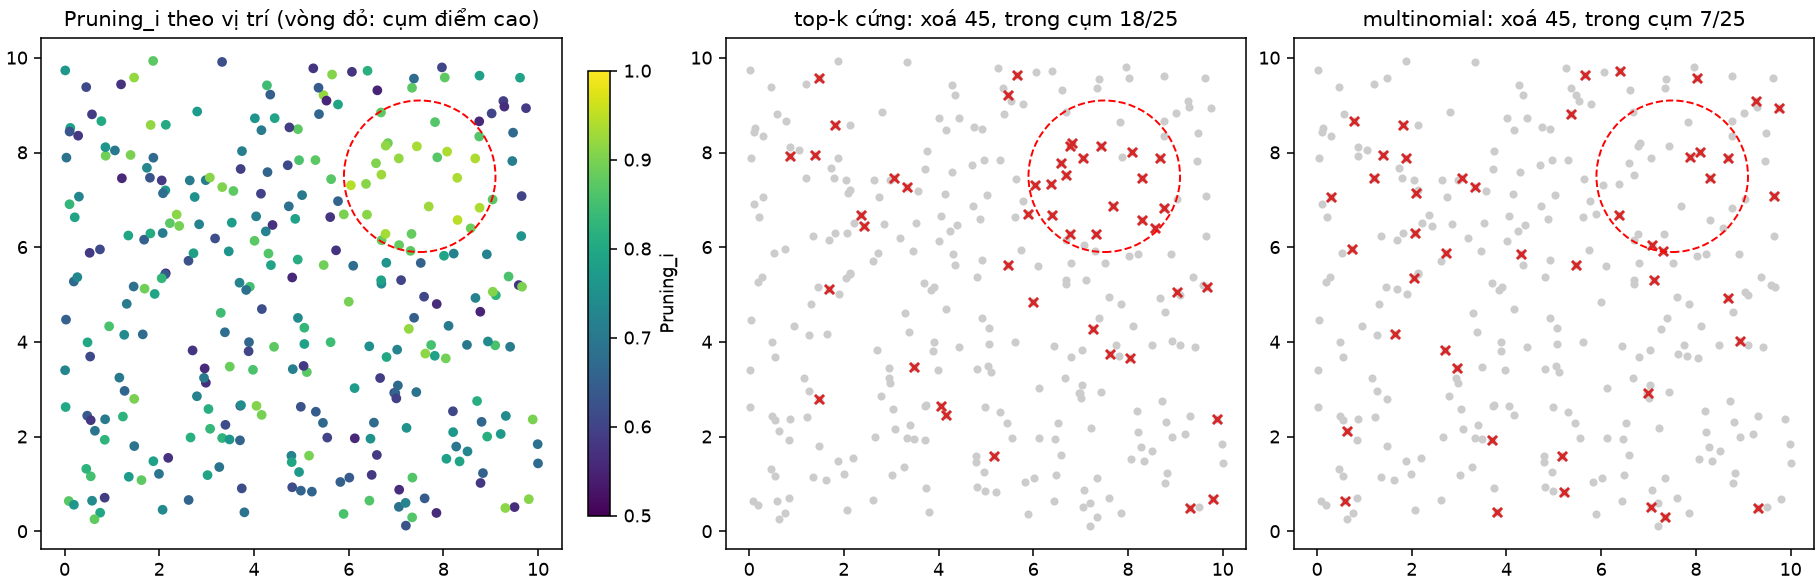
\includegraphics[width=0.68\linewidth]{5_4_tranh-xoa-ca-cum.png}
\captionof{figure}{\footnotesize Trái: bản đồ $P_i$ theo vị trí (vòng đỏ = cụm điểm cao). Giữa/phải: các điểm bị xoá bởi top-k cứng (xoá gần hết cụm) vs multinomial (rải rác hơn).}
\end{frame}

% --- 5_5_sigmoid-inverse.png ---
\begin{frame}{Sigmoid nghịch đảo (logit) để reset opacity}
\footnotesize
\begin{itemize}
    \item Tham số thực sự được tối ưu không phải $\alpha\in(0,1)$ mà là \texttt{\_opacity} (logit), với
    \[
    \alpha = \sigma(\text{logit}) = \frac{1}{1+e^{-\text{logit}}}, \qquad
    \text{logit} = \sigma^{-1}(\alpha) = \log\frac{\alpha}{1-\alpha}
    \]
    \item Khi cần ép/reset opacity về một giá trị nhỏ $\alpha_{\text{target}}$, ta phải gán lại \emph{logit}:
    \[
    \text{logit}_{\text{new}} = \sigma^{-1}(\min(\alpha,\alpha_{\text{target}}))
    \]
    vì gán trực tiếp lên $\alpha$ sẽ phá vỡ ràng buộc $(0,1)$ và làm sai gradient.
    \item Các mốc quan trọng: prune $\alpha=0{,}005$; reset $\alpha=0{,}01$; final prune $\alpha=0{,}1$; clamp $\alpha=0{,}8$.
    \item Bước $0{,}9\to 0{,}8$: logit $2{,}197 \to 1{,}386$ (bước nhỏ). Bước $0{,}9\to 0{,}01$: logit $2{,}197 \to -4{,}595$ (bước rất xa) $\Rightarrow$ reset là một cú "giật lùi" mạnh trong không gian logit.
\end{itemize}
\centering
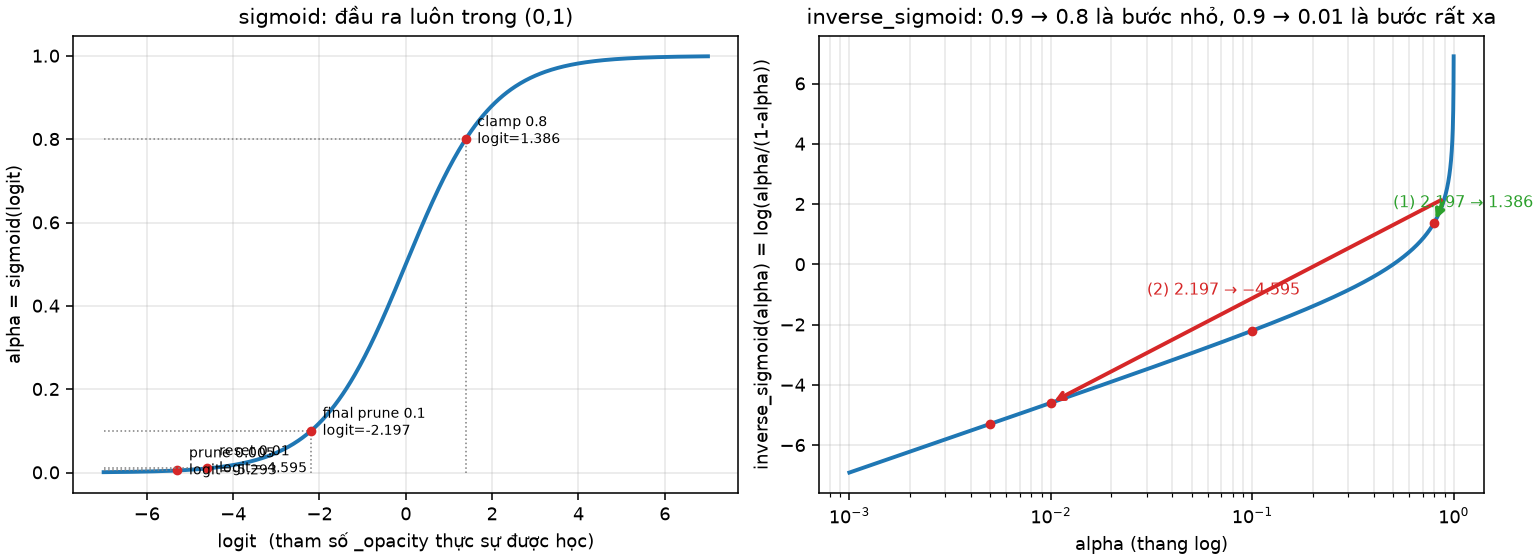
\includegraphics[width=0.68\linewidth]{5_5_sigmoid-inverse.png}
\captionof{figure}{\footnotesize Trái: hàm sigmoid với các mốc opacity đánh dấu trên trục logit. Phải: hàm nghịch đảo $\sigma^{-1}(\alpha)$ trên thang log của $\alpha$.}
\end{frame}

% --- 5_6_opacity-theo-iteration.png ---
\begin{frame}{Quỹ đạo opacity qua thời gian: tăng rồi bị reset định kỳ}
\footnotesize
\begin{itemize}
    \item Mô phỏng minh hoạ 4 Gaussian với "sức kéo" gradient khác nhau lên logit mỗi vòng: hữu ích ($k{=}+0{,}006$), trung bình ($k{=}+0{,}002$), vô dụng ($k{=}-0{,}001$), hồi sinh muộn ($k{=}0$ rồi $+0{,}004$ sau $t{=}7000$).
    \item Mỗi 100 vòng (trong khoảng $500<t<15000$), logit bị clamp: $\text{logit}\leftarrow\min(\text{logit}, \sigma^{-1}(0{,}8))$ -- ngăn opacity vượt $0{,}8$ ngay sau densify.
    \item Mỗi \texttt{opacity\_reset\_interval} $=3000$ vòng: $\text{logit}\leftarrow\min(\text{logit}, \sigma^{-1}(0{,}01))$ -- kéo \emph{toàn bộ} opacity về gần $0$, bất kể trước đó cao bao nhiêu.
    \item Sau reset, Gaussian hữu ích tự "leo" trở lại nhanh (gradient dương mạnh); Gaussian vô dụng rơi xuống dưới ngưỡng prune $\alpha=0{,}005$ và bị xoá ở lần prune multinomial kế tiếp.
    \item Cơ chế này cho các Gaussian "được nghi ngờ" một cơ hội chứng minh lại giá trị, thay vì xoá vĩnh viễn ngay lập tức.
\end{itemize}
\centering
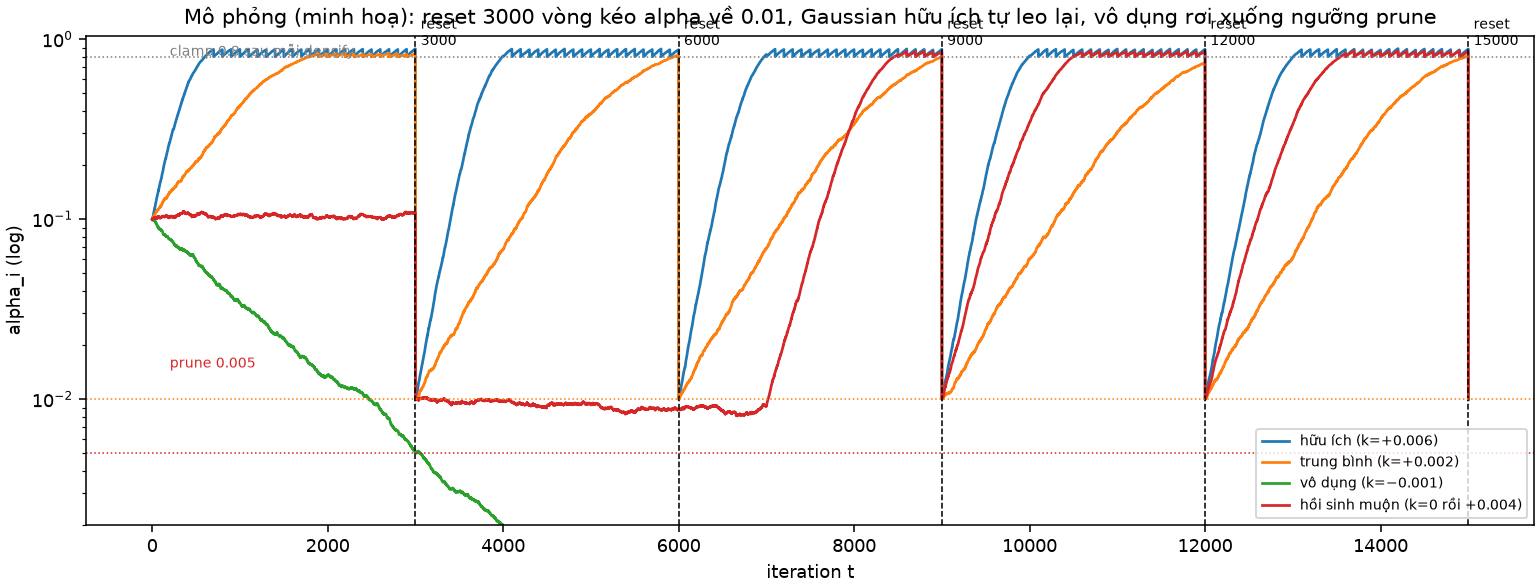
\includegraphics[width=0.72\linewidth]{5_6_opacity-theo-iteration.png}
\captionof{figure}{\footnotesize Quỹ đạo $\alpha_i(t)$ (log) của 4 Gaussian điển hình; các đường đứt nét đánh dấu mốc reset mỗi 3000 vòng, ngưỡng clamp 0,8 và ngưỡng prune 0,005.}
\end{frame}

% --- 5_7_histogram-truoc-sau-reset.png ---
\begin{frame}{Histogram phân bố opacity: trước và sau một lần reset}
\footnotesize
\begin{itemize}
    \item Mô phỏng $N=20000$ Gaussian: $60\%$ "hữu ích" có $\alpha_0\sim\text{Beta}(6,2)$ (thiên về giá trị cao), $40\%$ "lơ lửng" có $\alpha_0\sim\text{Beta}(1{,}5,4)$ (thiên về giá trị thấp).
    \item \textbf{Trước reset:} phân bố $\alpha_0$ đa dạng, trải rộng trên toàn khoảng $(0,1)$.
    \item \textbf{Ngay sau reset:} áp dụng $\text{logit}_1 = \min(\text{logit}_0, \sigma^{-1}(0{,}01))$ cho \emph{mọi} Gaussian $\Rightarrow$ toàn bộ phân bố dồn về sát $\alpha\approx 0{,}01$, gần như đồng nhất, mất hết sự đa dạng trước đó.
    \item \textbf{$\sim$500 vòng sau (minh hoạ):} nhóm hữu ích leo lại nhanh (gain trung bình $+3{,}5$ logit), nhóm vô dụng leo chậm hoặc đứng yên (gain trung bình $-0{,}3$ logit) $\Rightarrow$ phân bố tách lại thành hai nhóm.
    \item Tỉ lệ $\alpha<0{,}005$ (dưới ngưỡng prune) được ghi trực tiếp trên từng histogram để so sánh ba giai đoạn.
\end{itemize}
\centering
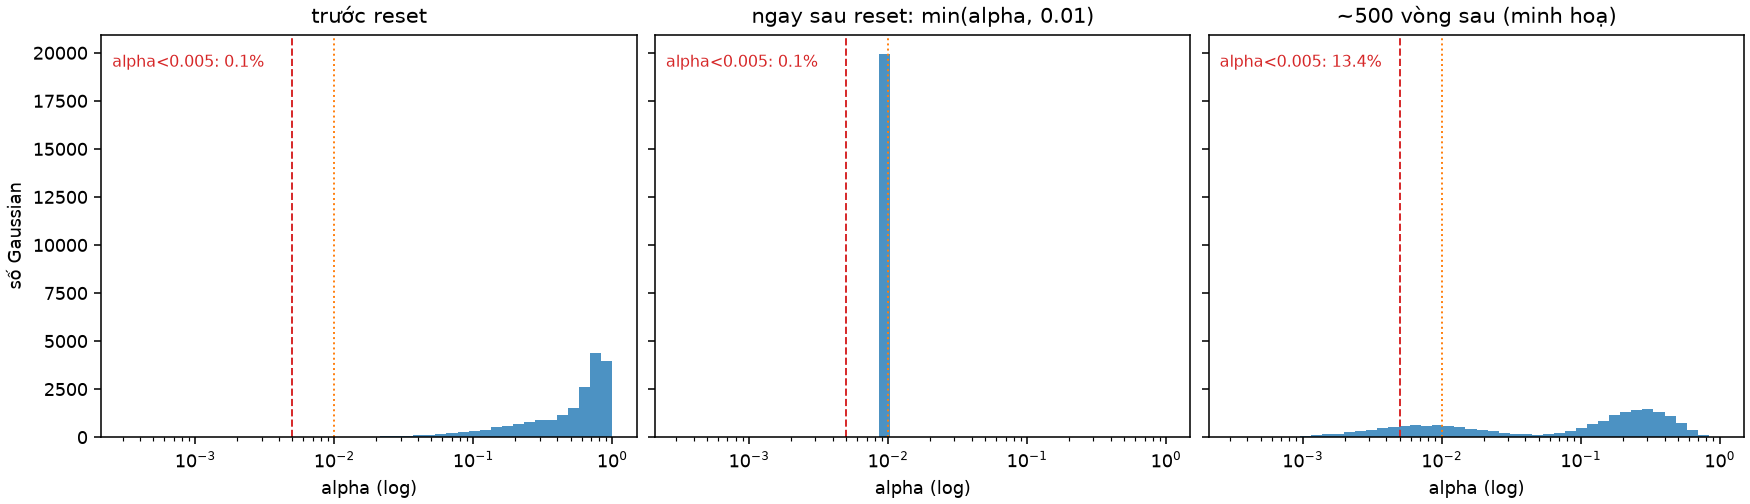
\includegraphics[width=0.85\linewidth]{5_7_histogram-truoc-sau-reset.png}
\captionof{figure}{\footnotesize Histogram $\alpha$ (thang log) trước reset, ngay sau reset, và $\sim$500 vòng sau reset; đường đứt = ngưỡng prune 0,005 và 0,01.}
\end{frame}

% --- 5_8_adam-sau-reset.png ---
\begin{frame}{Trạng thái Adam sau reset: có nên xoá luôn moment?}
\footnotesize
\begin{itemize}
    \item Adam cập nhật theo $m_t=\beta_1 m_{t-1}+(1-\beta_1)g$, $v_t=\beta_2 v_{t-1}+(1-\beta_2)g^2$, với bias-correction $\hat m_t = m_t/(1-\beta_1^t)$, $\hat v_t=v_t/(1-\beta_2^t)$, bước cập nhật $=\text{lr}\cdot \hat m_t/(\sqrt{\hat v_t}+\epsilon)$.
    \item Code thật (\texttt{replace\_tensor\_to\_optimizer}) khi reset opacity: đặt lại $(m,v)=(0,0)$ cho nhóm opacity, nhưng \textbf{không reset bộ đếm bước $t$ (step) của Adam} -- step vẫn tiếp tục từ giá trị cũ (vd. $t{=}6000$).
    \item Hệ quả: với $t$ lớn, $\beta_1^t\approx\beta_2^t\approx 0$ nên bias-correction gần như \emph{không còn hiệu lực đúng nghĩa} (được thiết kế cho $t$ nhỏ) $\Rightarrow$ bước cập nhật đầu tiên sau reset lớn bất thường, xấp xỉ
    \[
    \frac{\hat m_1}{\sqrt{\hat v_1}} \approx \frac{(1-\beta_1)g}{\sqrt{(1-\beta_2)g^2}} = \frac{0{,}1}{\sqrt{0{,}001}} \approx 3{,}16 \times \text{lr}
    \]
    \item So với Adam khởi tạo hoàn toàn mới (step$=0$, bias-correction đúng), phiên bản "giữ step" tạo một cú nhảy tham số lớn hơn nhiều ngay sau reset, rồi hội tụ dần về $1\times$lr ở trạng thái ổn định.
    \item Nếu không reset cả state Adam: optimizer "nhớ" quán tính cũ từ trước reset, có thể khiến opacity hồi phục lệch hướng hoặc chậm hơn dự kiến so với một khởi động sạch.
\end{itemize}
\centering
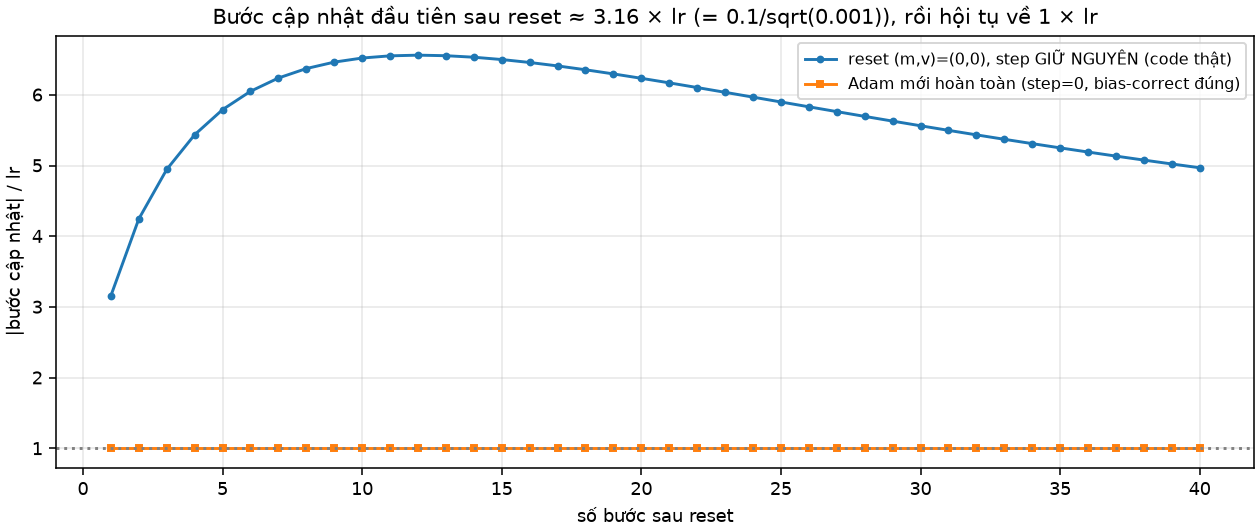
\includegraphics[width=0.6\linewidth]{5_8_adam-sau-reset.png}
\captionof{figure}{\footnotesize So sánh độ lớn bước cập nhật (chuẩn hoá theo lr) của Adam "giữ step cũ, reset $(m,v){=}(0,0)$" (code thật) vs Adam khởi tạo hoàn toàn mới.}
\end{frame}

% partADC_5b.tex --- ADC-5b: Final Prune, so sanh N(t), tong ket ADC
% Khong doc lap: khong co documentclass/usepackage/begin{document}

% --- 5_9_timeline-final-prune.png ---
\begin{frame}{Lịch chạy riêng của \texttt{final\_prune\_fastgs}}
\begin{itemize}
    \item Toàn bộ lịch trình huấn luyện $30\,000$ vòng chia làm hai vùng theo mốc \texttt{densify\_until\_iter} $= 15000$.
    \item \textbf{Vùng $t < 15000$}: densify + prune multinomial chạy mỗi $100$ vòng ($500 < t < 15000$, tổng cộng $145$ lần); \texttt{reset\_opacity} chạy khi $t \bmod 3000 = 0$ và $t < 15000$ ($5$ lần: $3000,\dots,15000$).
    \item \textbf{Vùng bảo vệ của final prune}: điều kiện chạy là
    \[
        15000 < \text{iteration} < 30000 \quad \text{và} \quad \text{iteration} \bmod 3000 = 0.
    \]
    \item Với điều kiện này, \texttt{final\_prune\_fastgs} chỉ thực sự chạy đúng \textbf{4 lần}: $t = 18000, 21000, 24000, 27000$.
    \item Mốc $t = 30000$ \textbf{không} chạy vì bất đẳng thức là chặt (\texttt{<}), không phải $\leq$; đây là lần huấn luyện cuối nên N giữ nguyên.
\end{itemize}
\begin{center}
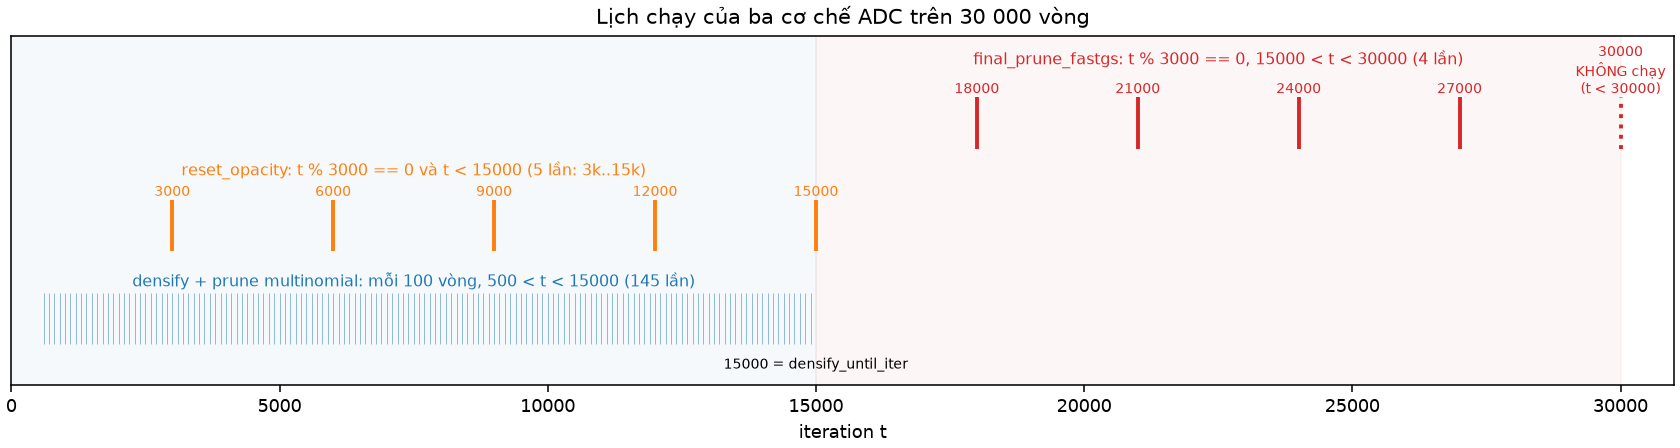
\includegraphics[width=0.75\linewidth]{5_9_timeline-final-prune.png}
\captionof{figure}{\footnotesize Lịch chạy của ba cơ chế ADC trên toàn bộ $30\,000$ vòng: densify/prune multinomial (xanh dương), reset opacity (cam), final prune (đỏ, 4 lần thực sự chạy tại 18k/21k/24k/27k).}
\end{center}
\end{frame}

% --- 5_10_vung-OR-final-prune.png ---
\begin{frame}{Điều kiện xoá cuối: phép OR, không phải AND}
\begin{columns}
\begin{column}{0.5\textwidth}
\footnotesize
\begin{itemize}
    \item Final prune xoá Gaussian $i$ nếu thoả \textbf{ít nhất một} trong hai tiêu chí:
    \[
        \text{xoá}_i = [\alpha_i < 0.1] \ \text{OR}\ [s_{p,i} > 0.9]
    \]
    với $\alpha_i = \text{sigmoid}(\text{opacity}_i)$, $s_{p,i} = \text{Pruning}_i$ (điểm số từ \texttt{compute\_gaussian\_score\_fastgs}).
    \item Đây là phép \textbf{OR}: chỉ cần opacity quá thấp \emph{hoặc} điểm số prune quá cao là bị loại — khác hẳn tập ứng viên $C$ ở prune giữa chừng, vốn kết hợp AND chặt với ngưỡng bán kính/scale.
    \item Ví dụ 5 Gaussian minh hoạ (từ chương 3): với $(\alpha, s_p)$ tương ứng, G3 bị xoá vì $s_p = 1.000 > 0.9$, G4 bị xoá vì $\alpha = 0.07 < 0.1$; G1, G2, G5 sống sót.
    \item Final prune \textbf{không lấy mẫu ngẫu nhiên} (không multinomial) — xoá thẳng toàn bộ tập thoả điều kiện, gọi trực tiếp \texttt{prune\_points} $\to$ \texttt{\_prune\_optimizer}.
\end{itemize}
\end{column}
\begin{column}{0.5\textwidth}
\centering
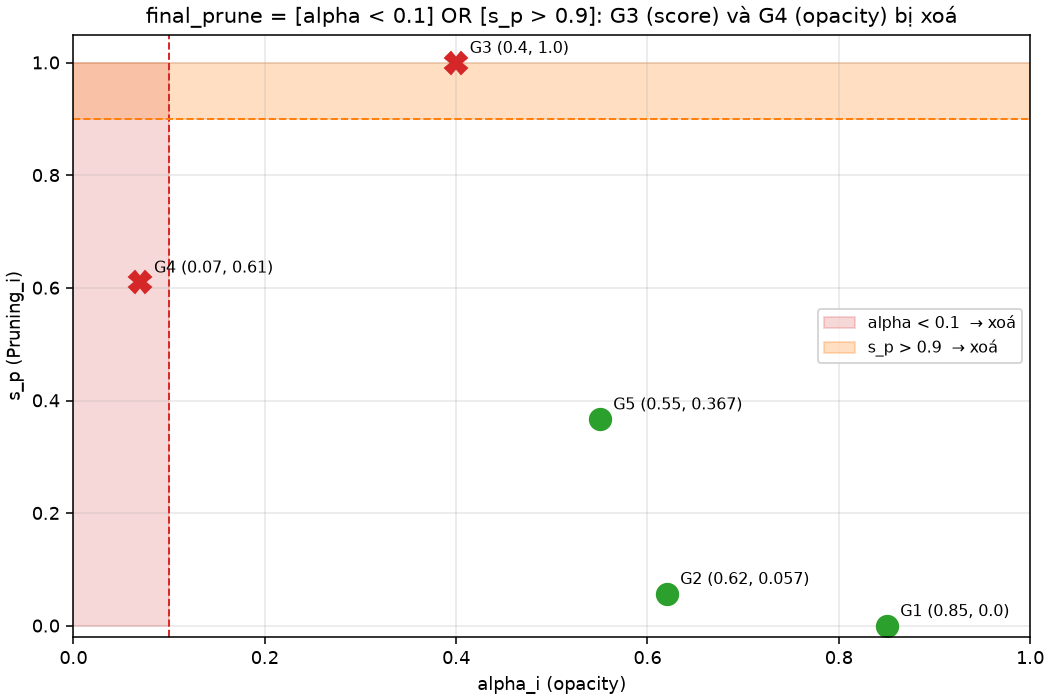
\includegraphics[width=\linewidth]{5_10_vung-OR-final-prune.png}
\captionof{figure}{\footnotesize Vùng OR trên mặt phẳng $(\alpha_i, s_{p,i})$: dải đỏ $\alpha<0.1$, dải cam $s_p>0.9$. G3 và G4 rơi vào vùng bị xoá, G1/G2/G5 sống sót.}
\end{column}
\end{columns}
\end{frame}

% --- 5_11_N-bac-thang-15k-30k.png ---
\begin{frame}{$N(t)$ dạng bậc thang trong giai đoạn $15000$--$30000$}
\begin{columns}[T]
\begin{column}{0.5\textwidth}
\scriptsize
\begin{itemize}
    \item Sau $t{=}15000$, densify không còn chạy $\Rightarrow$ $N$ chỉ giữ nguyên hoặc \textbf{giảm}.
    \item $N(t)$ dạng \textbf{bậc thang}: đoạn phẳng xen giữa các bước giảm tại $t{\in}\{18000,21000,24000,27000\}$ (final prune).
    \item Minh hoạ: $-12\%,-8\%,-5\%,-3\%$ từ $N_0{=}420{,}000$.
    \item Tại $t{=}30000$: không giảm nữa, đồ thị đi ngang — tách 2 chế độ: "tăng-giảm xen kẽ" trước $15000$, "chỉ giảm bậc thang" sau.
\end{itemize}
\end{column}
\begin{column}{0.5\textwidth}
\centering
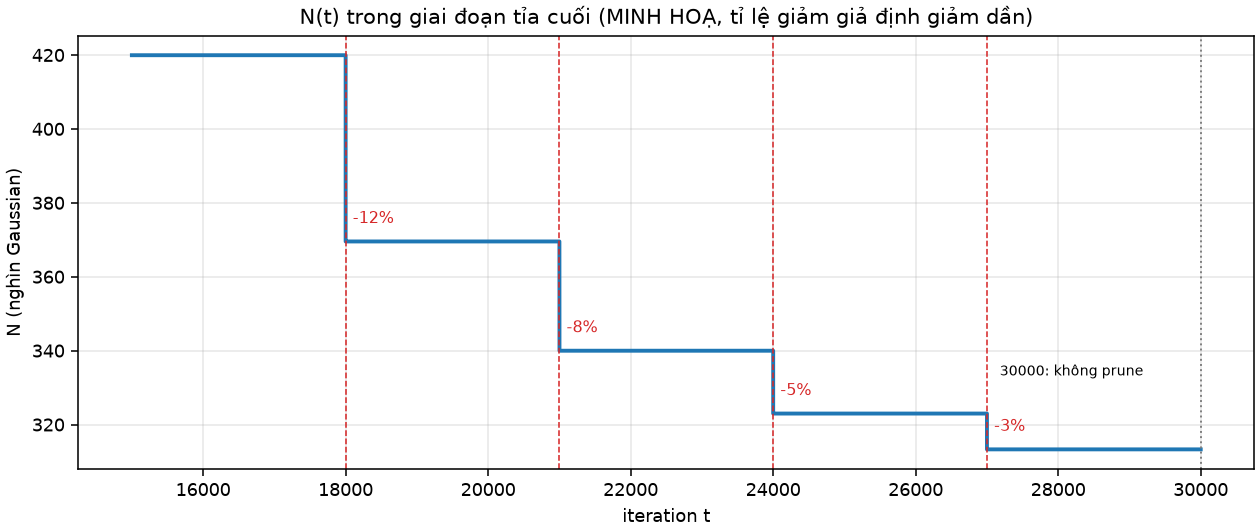
\includegraphics[width=0.95\linewidth]{5_11_N-bac-thang-15k-30k.png}
\captionof{figure}{\footnotesize $N(t)$ bậc thang trong $[15000,30000]$; đường đứt đỏ = final prune.}
\end{column}
\end{columns}
\end{frame}

% --- 5_12_radar-so-sanh.png ---
\begin{frame}{So sánh đa chiều: 3DGS vs FastGS-lite}
\footnotesize
\begin{itemize}
    \item Radar định tính (thang $0$--$3$, tự đặt) trên $6$ tiêu chí: số điều kiện densify, số điều kiện prune, mức ngẫu nhiên trong prune, có tỉa cuối hay không, chi phí render phụ mỗi lần densify, khả năng kiểm soát $N$.
    \item 3DGS gốc: điểm thấp ở hầu hết trục (densify $=2$, prune $=1$, ngẫu nhiên $=0$, tỉa cuối $=0$, chi phí render phụ $=0$, kiểm soát $N=1$).
    \item FastGS-lite: đạt điểm tối đa ($=3$) ở cả $6$ trục — nhiều tiêu chí hơn, có ngẫu nhiên hoá multinomial, có tỉa cuối, nhưng đổi lại chi phí render phụ để tính importance/pruning score.
    \item Số liệu tham chiếu (chương 13, minh hoạ): $N$ trung bình $3$DGS $\approx 933$ nghìn so với FastGS-lite $\approx 293$ nghìn; $R_{\text{gauss}}$ (tỉ lệ Gaussian giữ lại) $= 1.0$ với 3DGS so với $0.314$ với FastGS-lite (giả định); chi phí render phụ mỗi lần densify: $0$ với 3DGS, $\approx 20$ với FastGS-lite.
    \item Kết luận định tính: FastGS-lite đánh đổi chi phí tính điểm số để đạt $N$ nhỏ hơn đáng kể và kiểm soát chặt hơn.
\end{itemize}
\begin{center}
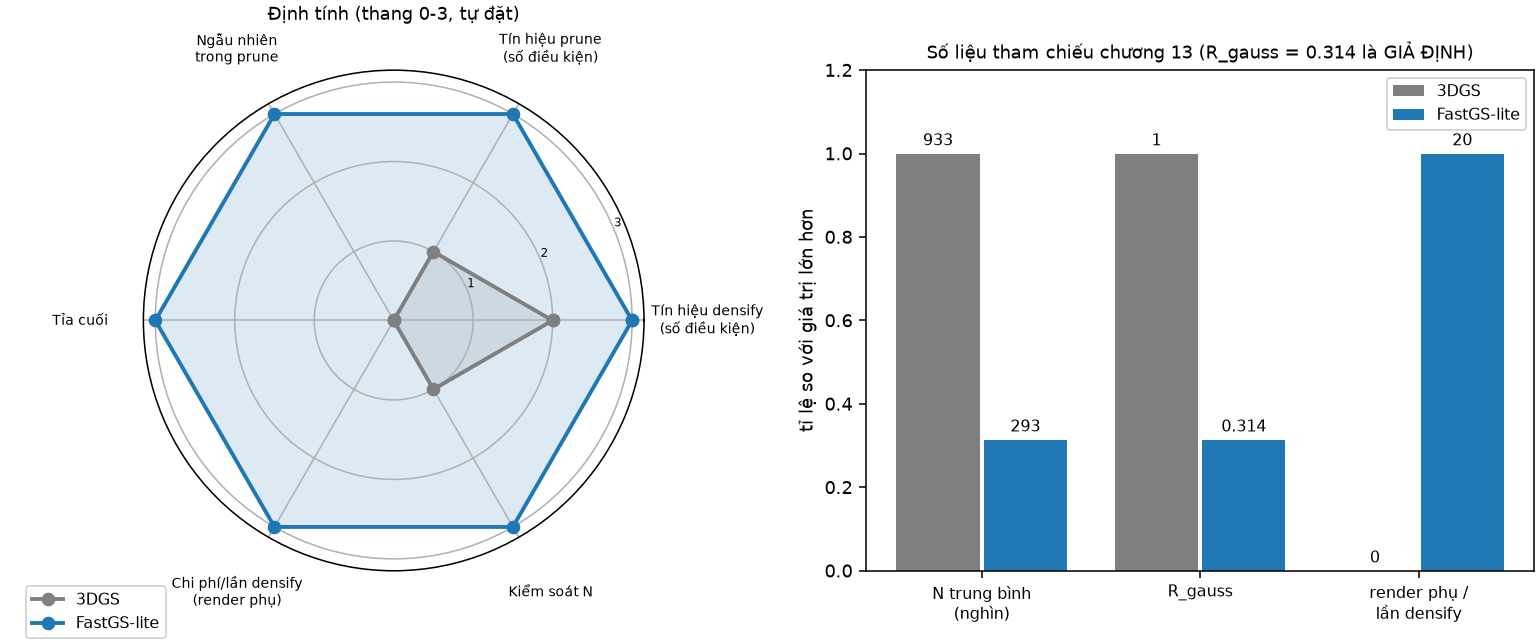
\includegraphics[width=0.7\linewidth]{5_12_radar-so-sanh.png}
\captionof{figure}{\footnotesize Trái: radar định tính 6 tiêu chí. Phải: số liệu tham chiếu $N$ trung bình, $R_{\text{gauss}}$, chi phí render phụ (chuẩn hoá theo giá trị lớn hơn).}
\end{center}
\end{frame}

% --- 5_13_N-t-3dgs-vs-fastgs.png ---
\begin{frame}{$N(t)$: 3DGS gốc so với FastGS-lite trên cùng trục thời gian}
\begin{columns}
\begin{column}{0.55\textwidth}
\footnotesize
\begin{itemize}
    \item Mô hình minh hoạ: cùng $N_0 = 100\,000$, cùng lịch chạy ($500 < t < 15000$, mỗi $100$ vòng), nhưng khác hệ số $(r_{\text{spawn}}, r_{\text{prune}}, r_{\text{reset}})$:
    \[
        N_{t} = N_{t-1}\,(1+r_{\text{spawn}})(1-r_{\text{prune}})
    \]
    áp dụng mỗi $100$ vòng, cộng thêm hệ số giảm tại mỗi lần reset opacity ($t \bmod 3000=0,\ t<15000$).
    \item 3DGS (minh hoạ): $r_{\text{spawn}}=0.0227$, $r_{\text{prune}}=0.003$, giảm reset $4\%$, \textbf{không} có final prune $\Rightarrow$ TB $\approx 933$k Gaussian.
    \item FastGS-lite (minh hoạ): $r_{\text{spawn}}=0.0155$, $r_{\text{prune}}=0.004$, giảm reset $4\%$, \textbf{có} final prune tại $18000/21000/24000/27000$ với tỉ lệ $12\%/8\%/5\%/3\%$ $\Rightarrow$ TB $\approx 293$k Gaussian.
    \item FastGS-lite hội tụ về $N$ nhỏ hơn rõ rệt nhờ tốc độ spawn thấp hơn \emph{và} có thêm giai đoạn tỉa cuối mà 3DGS không có.
\end{itemize}
\end{column}
\begin{column}{0.45\textwidth}
\centering
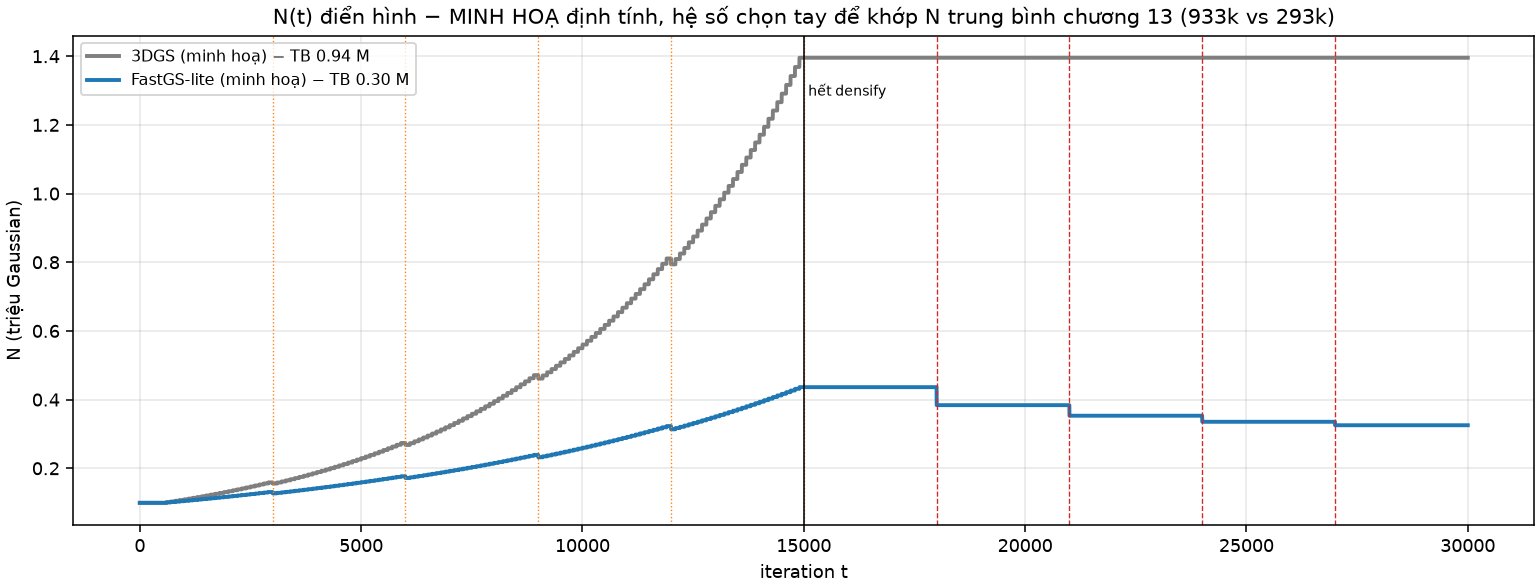
\includegraphics[width=\linewidth]{5_13_N-t-3dgs-vs-fastgs.png}
\captionof{figure}{\footnotesize $N(t)$ minh hoạ định tính: 3DGS (xám) tăng liên tục đến TB $\approx 0.93$M; FastGS-lite (xanh) có bậc thang giảm sau $15000$, TB $\approx 0.29$M.}
\end{column}
\end{columns}
\end{frame}

% --- 5_14_optimizer-cat-ghep.png ---
\begin{frame}{Cắt/ghép trạng thái Adam khi $N$ thay đổi}
\tiny
\begin{itemize}
    \item Adam lưu $(m,v){=}(\text{exp\_avg},\text{exp\_avg\_sq})$ mỗi hàng (Gaussian). $N$ đổi $\Rightarrow$ tensor này phải cắt/ghép đồng bộ.
    \item \textbf{Thêm (clone/split)}: nối hàng mới, con nhận $(m,v){=}(0,0)$, nhưng \texttt{step} Adam dùng chung $\Rightarrow$ bias-correction ${\approx}1$ ngay dù step đã lớn.
    \item \textbf{Xoá (prune)}: giữ hàng theo mặt nạ, loại đúng $(m,v)$ của Gaussian bị xoá, không xáo trộn thứ tự còn lại.
    \item \textbf{Ép opacity}: chỉ nhóm opacity bị thay $(m,v){\leftarrow}(0,0)$; các nhóm khác (xyz/SH/scale/rotation) giữ nguyên. Áp dụng sau densify và tại mỗi lần reset.
    \item \texttt{step} của Adam \textbf{không} bị reset trong mọi trường hợp.
\end{itemize}
\centering
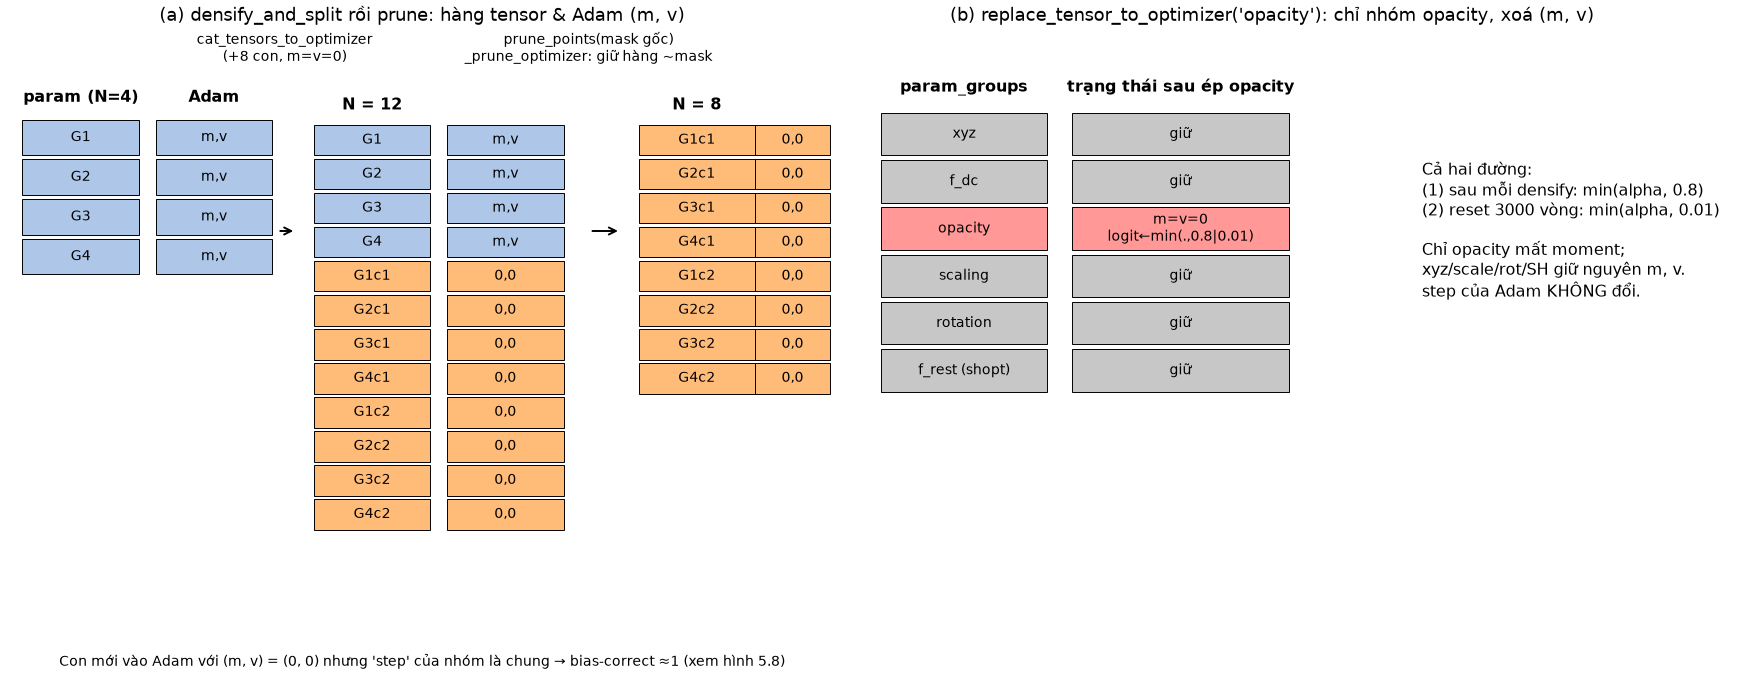
\includegraphics[width=0.55\linewidth]{5_14_optimizer-cat-ghep.png}
\captionof{figure}{\footnotesize (a) split rồi prune: nối rồi cắt theo mask. (b) replace opacity: chỉ nhóm opacity mất $(m,v)$.}
\end{frame}

% --- 5_15_so-do-khoi-ADC.png ---
\begin{frame}{Sơ đồ khối tổng thể của Adaptive Density Control}
\tiny
\begin{itemize}
    \item Vòng lặp khép kín: tích luỹ thống kê $\to$ tính điểm số $\to$ densify (AND) $\to$ prune multinomial $\to$ ép opacity $\to$ reset opacity $\to$ final prune (OR) $\to$ cập nhật tensor.
    \item \textbf{Mỗi vòng $t{<}15000$}: \texttt{add\_densification\_stats} cập nhật \texttt{max\_radii2D}, \texttt{accum}, \texttt{denom}.
    \item \textbf{Mỗi 100 vòng}: score trên $V{=}10$ view $\to$ Importance, Pruning; \textbf{DENSIFY (AND)}: clone khi $|g|{\geq}2{\times}10^{-4}$, split khi $|g_{\text{abs}}|{\geq}1.2{\times}10^{-3}$, cả hai cần Imp${>}5$.
    \item \textbf{PRUNE MULTINOMIAL}: $C{=}\{\alpha{<}0.005 \mid r_{2D}{>}20 \mid \max s{>}0.1{\cdot}\text{extent}\}$, $w{=}1/(10^{-6}{+}1{-}\text{Pruning})$, xoá $S{\sim}\text{multinomial}(w)$.
    \item \textbf{RESET} mỗi 3000 vòng: $\text{logit}{\leftarrow}\text{inv\_sigmoid}(\min(\alpha,0.01))$; \textbf{FINAL PRUNE} ($15000{<}t{<}30000$): xoá$=[\alpha{<}0.1]$ OR $[\text{Pruning}{>}0.9]$.
    \item Sau mỗi lần gọi: các tensor thống kê reset về 0; \texttt{step} Adam không reset.
\end{itemize}
\centering
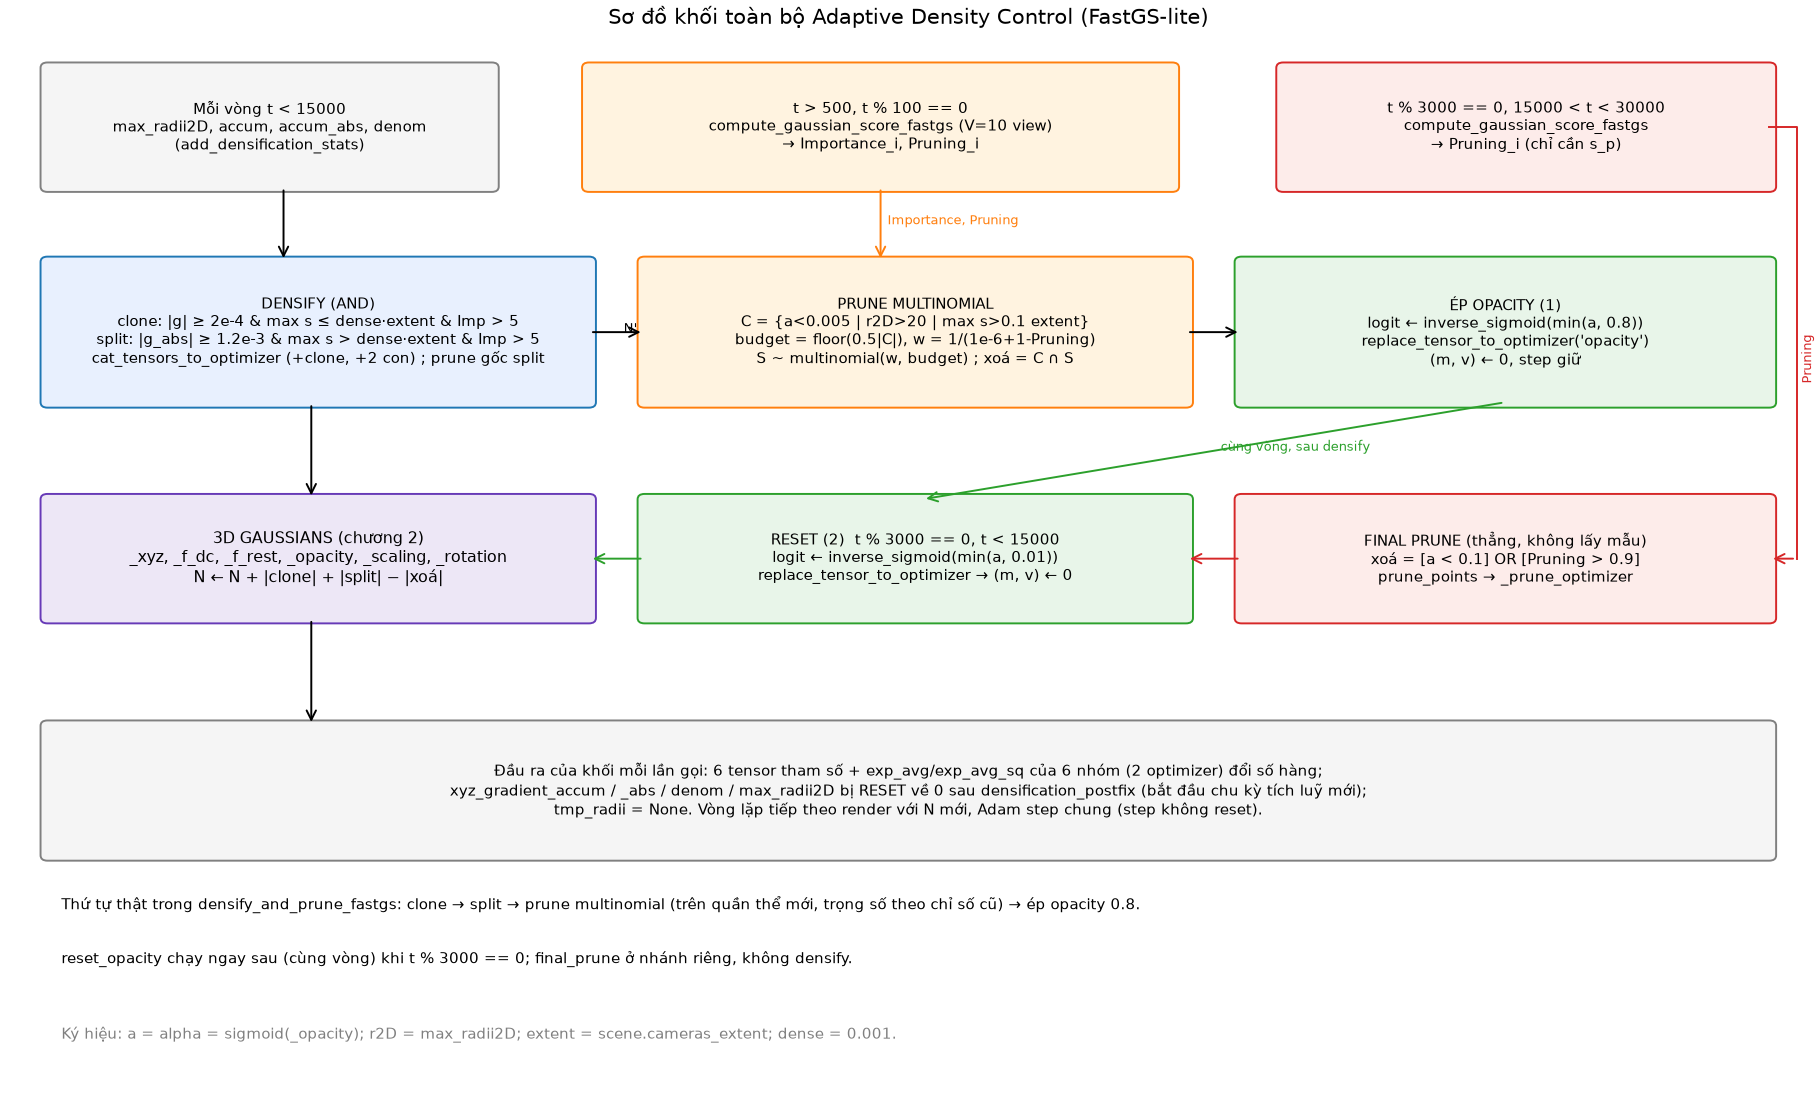
\includegraphics[width=0.42\linewidth]{5_15_so-do-khoi-ADC.png}
\captionof{figure}{\footnotesize Sơ đồ khối toàn bộ ADC.}
\end{frame}

% --- 5_16_thu-tu-that-code.png ---
\begin{frame}{Thứ tự thực thi thật trong code (khác thứ tự lý thuyết)}
\begin{columns}
\begin{column}{0.5\textwidth}
\footnotesize
\begin{itemize}
    \item Thứ tự thật trong \texttt{densify\_and\_prune\_fastgs}: \textbf{clone $\to$ split $\to$ prune multinomial} (trên quần thể \emph{mới}, trọng số vẫn theo \emph{chỉ số cũ}) $\to$ ép opacity $0.8$.
    \item Ví dụ kiểm định: cảnh $4$ Gaussian, $t>3000$, cả $4$ đều split $\to N=8$ con; \texttt{max\_radii2D} của con $=0$ nhưng $\max s$ của con $=s/1.6 > 0.169$ nên cả $8$ đều vào tập ứng viên $C$ ($|C|=8$, budget $=4$).
    \item \texttt{padded\_importance[:4]} $=$ trọng số cũ của $4$ Gaussian gốc; $4$ vị trí còn lại (con thứ hai) là $0$ $\Rightarrow$ \texttt{multinomial(w, 4)} bắt buộc rút đúng $\{0,1,2,3\}$.
    \item Kết quả: xoá $= C\cap S = \{$G1c1, G2c1, G3c1, G4c1$\}$ $\Rightarrow N=4$ (thay vì công thức lý thuyết chương $7.8$ dự đoán $4+0+4-2=6$).
    \item Trong huấn luyện thật, tỉ lệ Gaussian bị split mỗi lần chỉ vài phần trăm nên độ lệch giữa lý thuyết và thực thi là nhỏ, nhưng cơ chế "trọng số cũ gán theo chỉ số" vẫn tồn tại và cần lưu ý khi debug.
\end{itemize}
\end{column}
\begin{column}{0.5\textwidth}
\centering
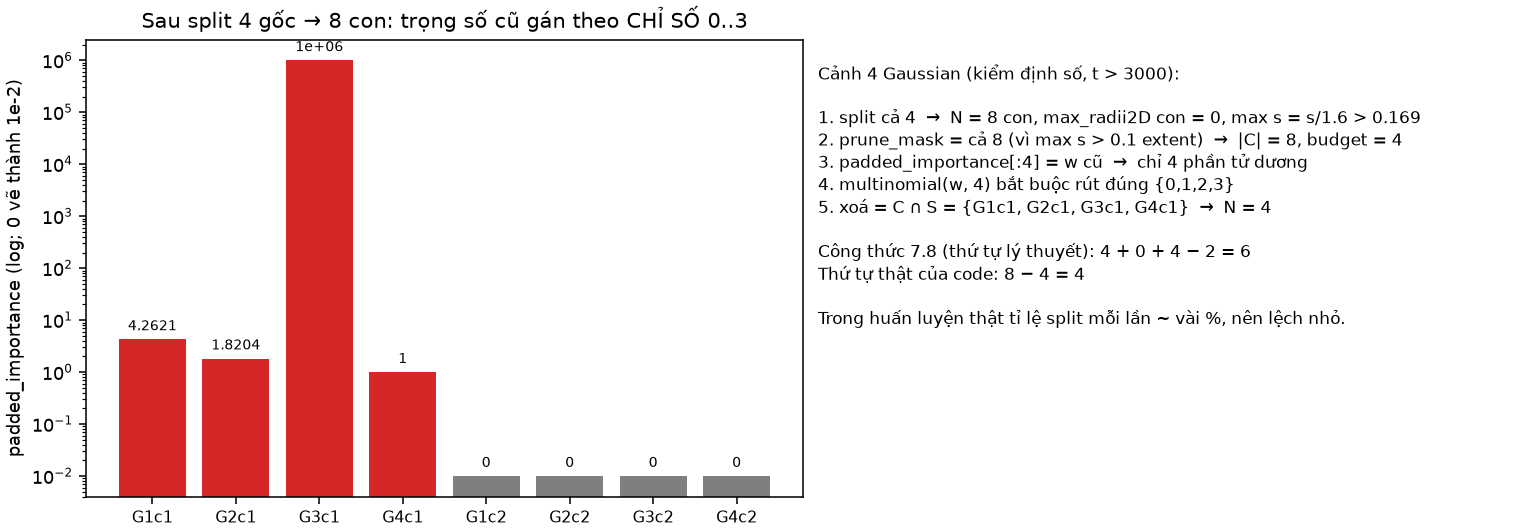
\includegraphics[width=\linewidth]{5_16_thu-tu-that-code.png}
\captionof{figure}{\footnotesize Trái: trọng số \texttt{padded\_importance} sau split — $4$ con đầu nhận trọng số cũ (đỏ), $4$ con sau bằng $0$ (xám). Phải: diễn giải từng bước dẫn đến $N=4$ thay vì $6$ theo công thức lý thuyết.}
\end{column}
\end{columns}
\end{frame}


\section{ADC chuyên sâu — P6: Toy Model 2D (Có ADC vs Không ADC)}
% partADC_6.tex — Phan 6: Adaptive Density Control minh hoa qua toy model 2D
% Chi chua cac khoi frame, khong documentclass/usepackage/begin{document}.

% --- 6_1_muc-tieu-va-gaussian-2d.png ---
\begin{frame}{Toy model 2D: mục tiêu và một Gaussian}
\begin{itemize}
    \footnotesize
    \item Ảnh mục tiêu $64\times 64$ px: một hình tròn phẳng (màu đều) + vùng chi tiết (dải mảnh 2 px, 5 chấm màu xen kẽ, ô vuông nhỏ).
    \item Mỗi Gaussian 2D: $G(x) = \exp\!\big(-\tfrac{1}{2}d^\top \Sigma^{-1} d\big)$, với $d = x - \mu$, $\Sigma$ tham số hoá bởi scale $s=(s_1,s_2)$ và góc xoay $\theta$.
    \item Footprint (vùng Gaussian được phép chạm) giới hạn ở $3\sigma$, tức $d^\top\Sigma^{-1}d < 9$ — ngoài phạm vi này chỉ còn màu nền.
    \item Render bằng alpha-compositing theo thứ tự chỉ số (độ sâu): $I(x) = \sum_i T_i\,\alpha_i G_i(x)\,c_i + T_{\text{end}}\cdot\text{bg}$, với $T_i = \prod_{j<i}(1-\alpha_j G_j)$.
\end{itemize}
\begin{center}
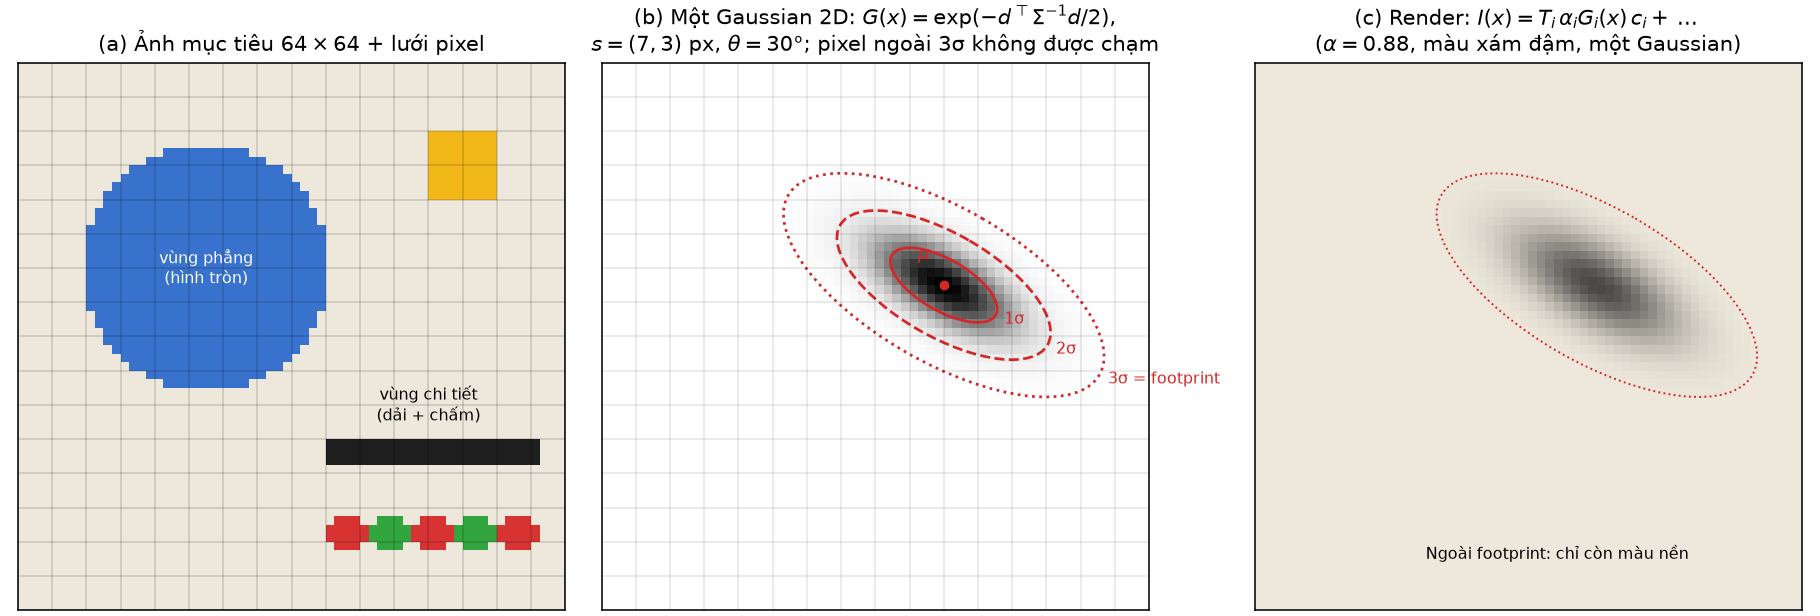
\includegraphics[width=0.75\linewidth]{6_1_muc-tieu-va-gaussian-2d.png}
\captionof{figure}{\footnotesize (a) Ảnh mục tiêu + lưới pixel; (b) một Gaussian $s=(7,3)$ px, $\theta=30°$ với các đường mức $1\sigma,2\sigma,3\sigma$; (c) kết quả render của Gaussian đó lên nền.}
\end{center}
\end{frame}

% --- 6_2_thieu-gaussian.png ---
\begin{frame}{Trường hợp thiếu Gaussian (under-reconstruction)}
\begin{itemize}
    \footnotesize
    \item Khởi tạo toy chỉ với 6 Gaussian nhỏ ($s=3$ px), rải rác không đủ để phủ vùng chi tiết (dải + chấm + ô vuông).
    \item Sai số $|I-T|$ (trung bình 3 kênh) lớn tại đúng những vùng không có Gaussian nào chạm tới.
    \item Gradient vị trí $-\nabla_\mu L$ tại mỗi Gaussian có độ lớn $\|\nabla_\mu\|$ vượt ngưỡng clone toy $\tau_{\text{grad}} = 4\times 10^{-5}$.
    \item Đây chính là tín hiệu để ADC quyết định \textbf{CLONE}: Gaussian di chuyển không đủ nhanh để tự phủ hết vùng thiếu, cần thêm bản sao.
\end{itemize}
\begin{center}
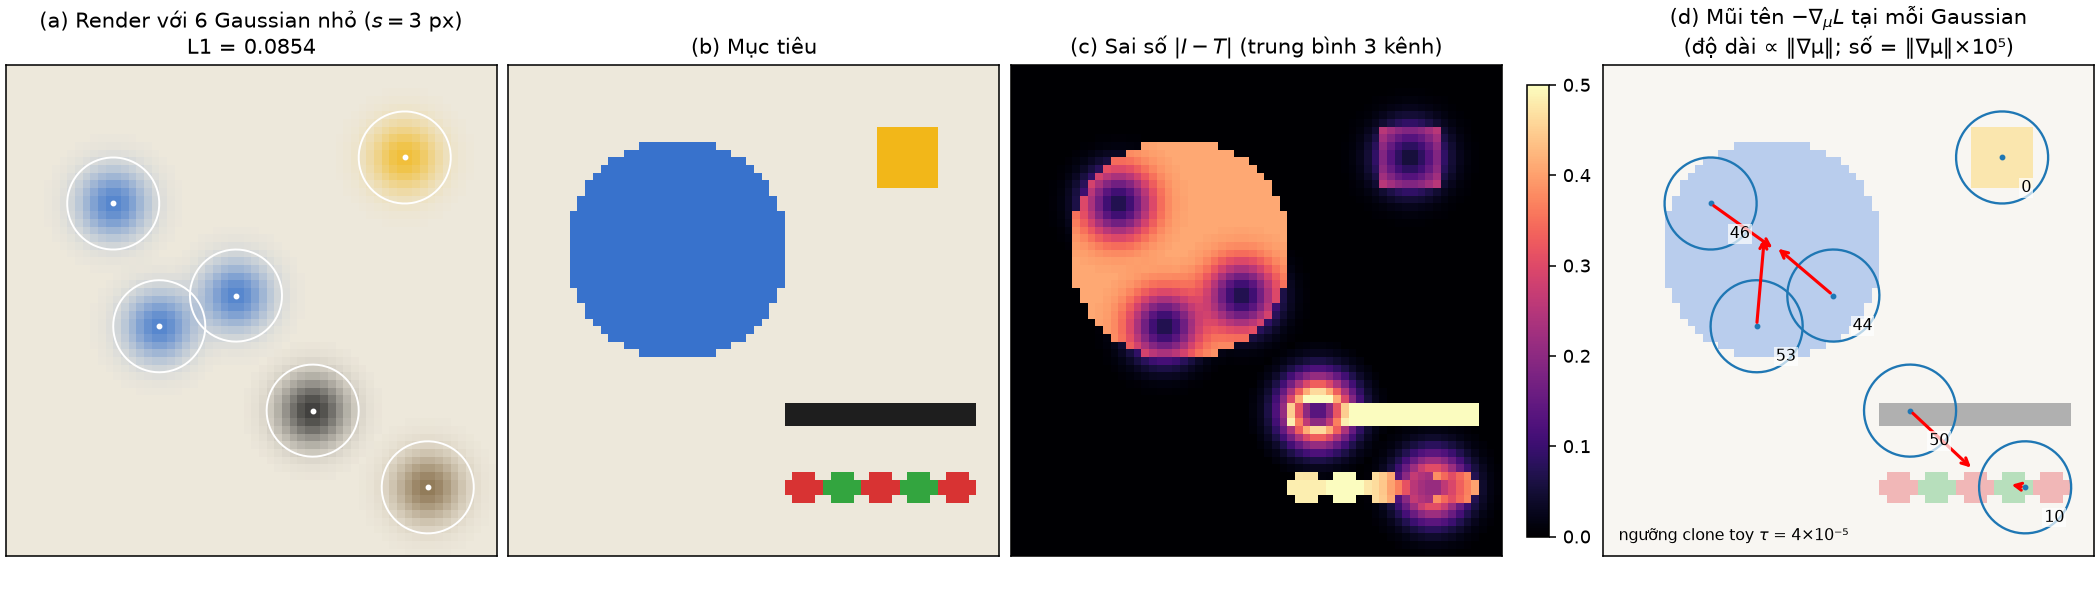
\includegraphics[width=0.75\linewidth]{6_2_thieu-gaussian.png}
\captionof{figure}{\footnotesize (a) Render với 6 Gaussian nhỏ; (b) mục tiêu; (c) bản đồ sai số; (d) mũi tên $-\nabla_\mu L$ và giá trị $\|\nabla_\mu\|\times 10^5$ tại từng Gaussian.}
\end{center}
\end{frame}

% --- 6_3_du-gaussian-qua-to.png ---
\begin{frame}{Trường hợp Gaussian dư / quá to (over-reconstruction)}
\begin{itemize}
    \footnotesize
    \item Một Gaussian duy nhất, kích thước lớn $s=(13,\ 6.5)$ px, cố phủ toàn bộ vùng chi tiết (dải + 5 chấm) cùng lúc.
    \item Sai số mờ đều trên toàn vùng, sai cả tại chấm lẫn khoảng trống — Gaussian quá to không tái tạo được chi tiết cục bộ.
    \item Ngưỡng phân loại ``to'': $\max_k s_k > S_{\text{big}} = 3.5$ px.
    \item Chỉ số quyết định split dùng \emph{tổng trị tuyệt đối} gradient theo pixel $\sum_x |g_x|$ (ngưỡng $\tau_{\text{abs}}=4\times 10^{-4}$), lớn hơn nhiều lần so với tổng có dấu $\|\sum_x g_x\|$ — vì các mũi tên gradient trong footprint kéo về nhiều phía trái ngược nhau.
\end{itemize}
\begin{center}
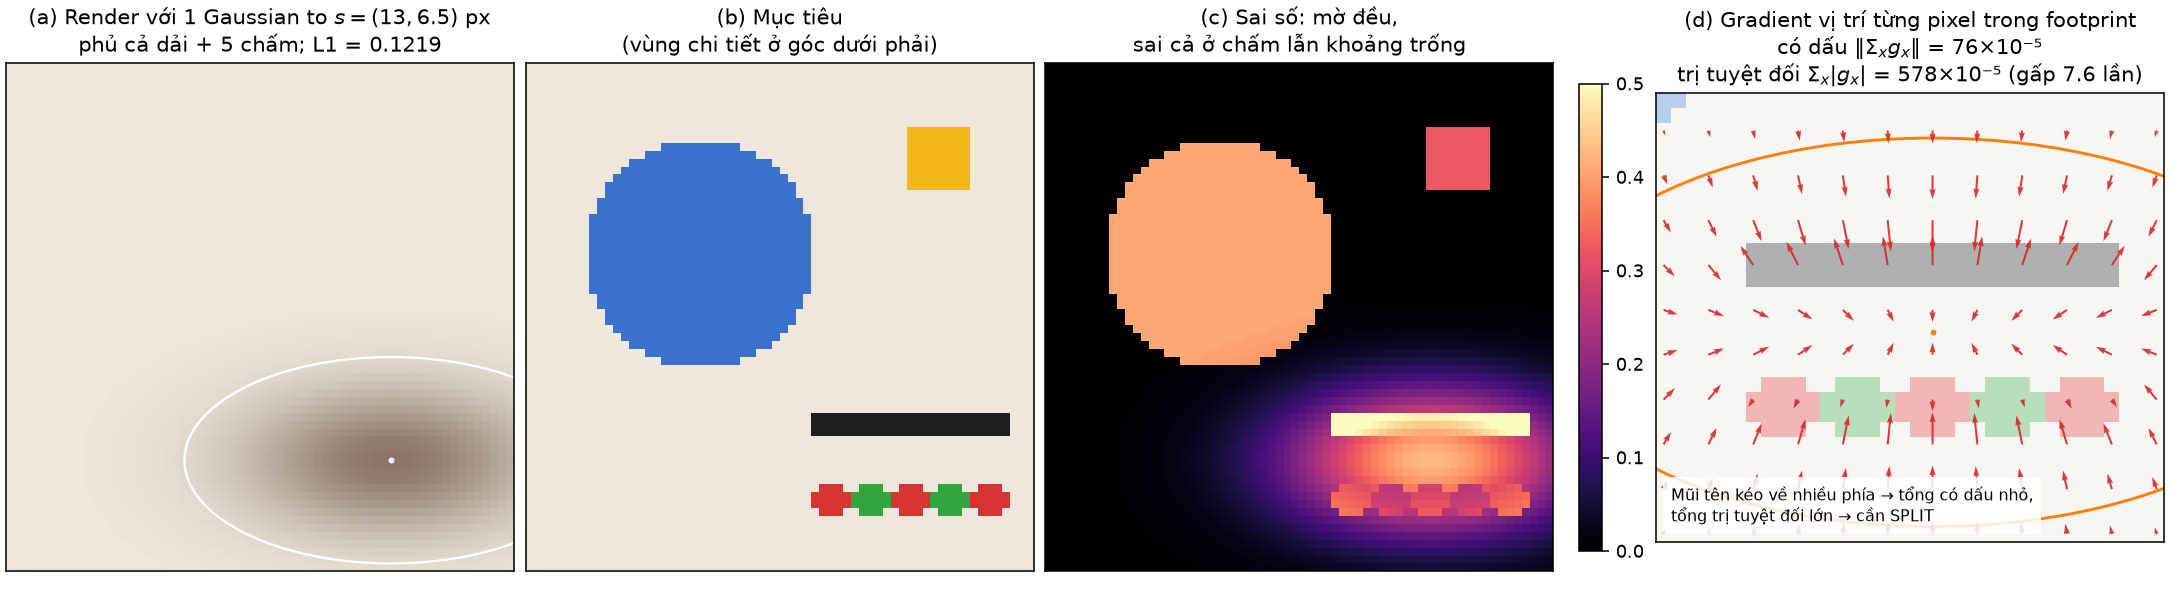
\includegraphics[width=0.75\linewidth]{6_3_du-gaussian-qua-to.png}
\captionof{figure}{\footnotesize (a) Render với 1 Gaussian to; (b) mục tiêu; (c) sai số mờ đều; (d) gradient theo từng pixel — tổng có dấu nhỏ nhưng tổng trị tuyệt đối lớn $\Rightarrow$ \textbf{SPLIT}.}
\end{center}
\end{frame}

% --- 6_4_clone-truoc-sau.png ---
\begin{frame}{CLONE: sao chép nguyên trạng Gaussian thiếu}
\begin{itemize}
    \footnotesize
    \item Trước clone: 1 Gaussian nhỏ có $\|\nabla_\mu\| \ge \tau$, cần phủ vùng rộng hơn kích thước hiện tại.
    \item CLONE tạo bản sao \emph{y hệt} (cùng $\mu,\Sigma,c,\alpha$); trạng thái Adam của bản mới được khởi tạo lại $m=v=0$ trong khi bản gốc giữ nguyên lịch sử — nên hai bản dịch chuyển khác tốc độ.
    \item Ngay sau clone hai bản trùng khít nhau; sau khoảng 120 bước Adam, quỹ đạo $\mu$ của bản gốc và bản sao tách rời để mỗi bản phủ một phần vùng cần thiết.
    \item Kết quả: loss L1 giảm rõ rệt sau khi hai bản tách ra và chia nhau vùng phủ.
\end{itemize}
\begin{center}
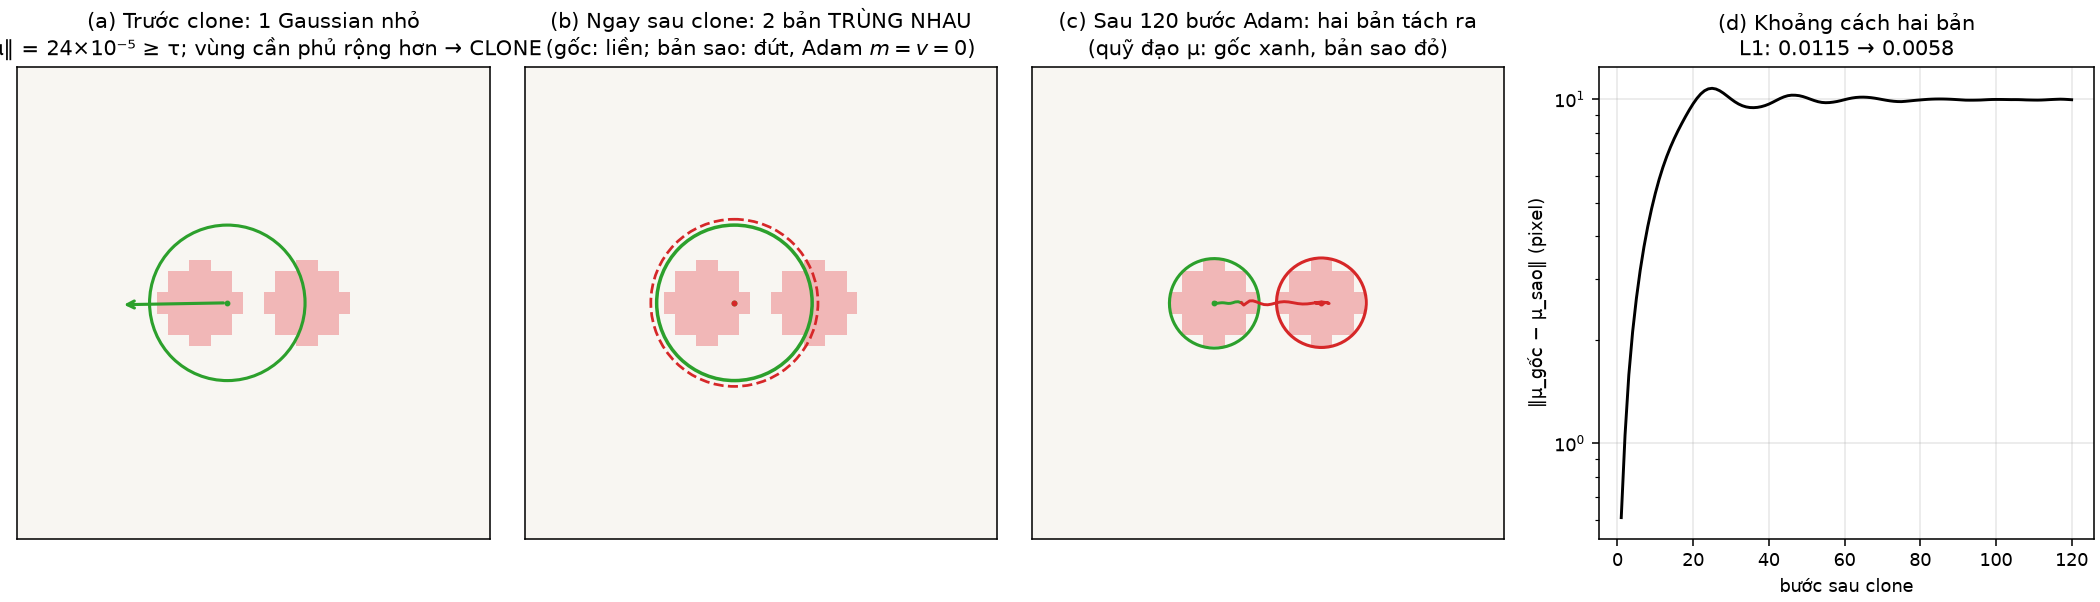
\includegraphics[width=0.75\linewidth]{6_4_clone-truoc-sau.png}
\captionof{figure}{\footnotesize (a) Trước clone; (b) ngay sau clone — 2 bản trùng nhau; (c) sau 120 bước — hai bản tách ra; (d) khoảng cách $\|\mu_{\text{gốc}}-\mu_{\text{sao}}\|$ theo bước, cùng L1 trước/sau.}
\end{center}
\end{frame}

% --- 6_5_split-truoc-sau.png ---
\begin{frame}{SPLIT: tách Gaussian quá to thành các con nhỏ hơn}
\begin{columns}[T]
\begin{column}{0.52\textwidth}
\scriptsize
\begin{itemize}
    \item $n_{\text{child}}{=}2$ con lấy mẫu từ hình dạng gốc: $\mu_{\text{con}}{=}\mu+R\epsilon^{(j)}$, $\epsilon^{(j)}{\sim}\mathcal{N}(0,\text{diag}(s^2))$.
    \item Scale mỗi con giảm còn $s/1.6$; Gaussian gốc bị \textbf{xoá}.
    \item Ngay sau split, loss \emph{xấu tạm thời}; sau 150 bước Adam mỗi con tự định vị lại.
    \item Kết quả cuối: L1 giảm, chi tiết cục bộ khôi phục tốt hơn 1 Gaussian to.
\end{itemize}
\end{column}
\begin{column}{0.48\textwidth}
\centering
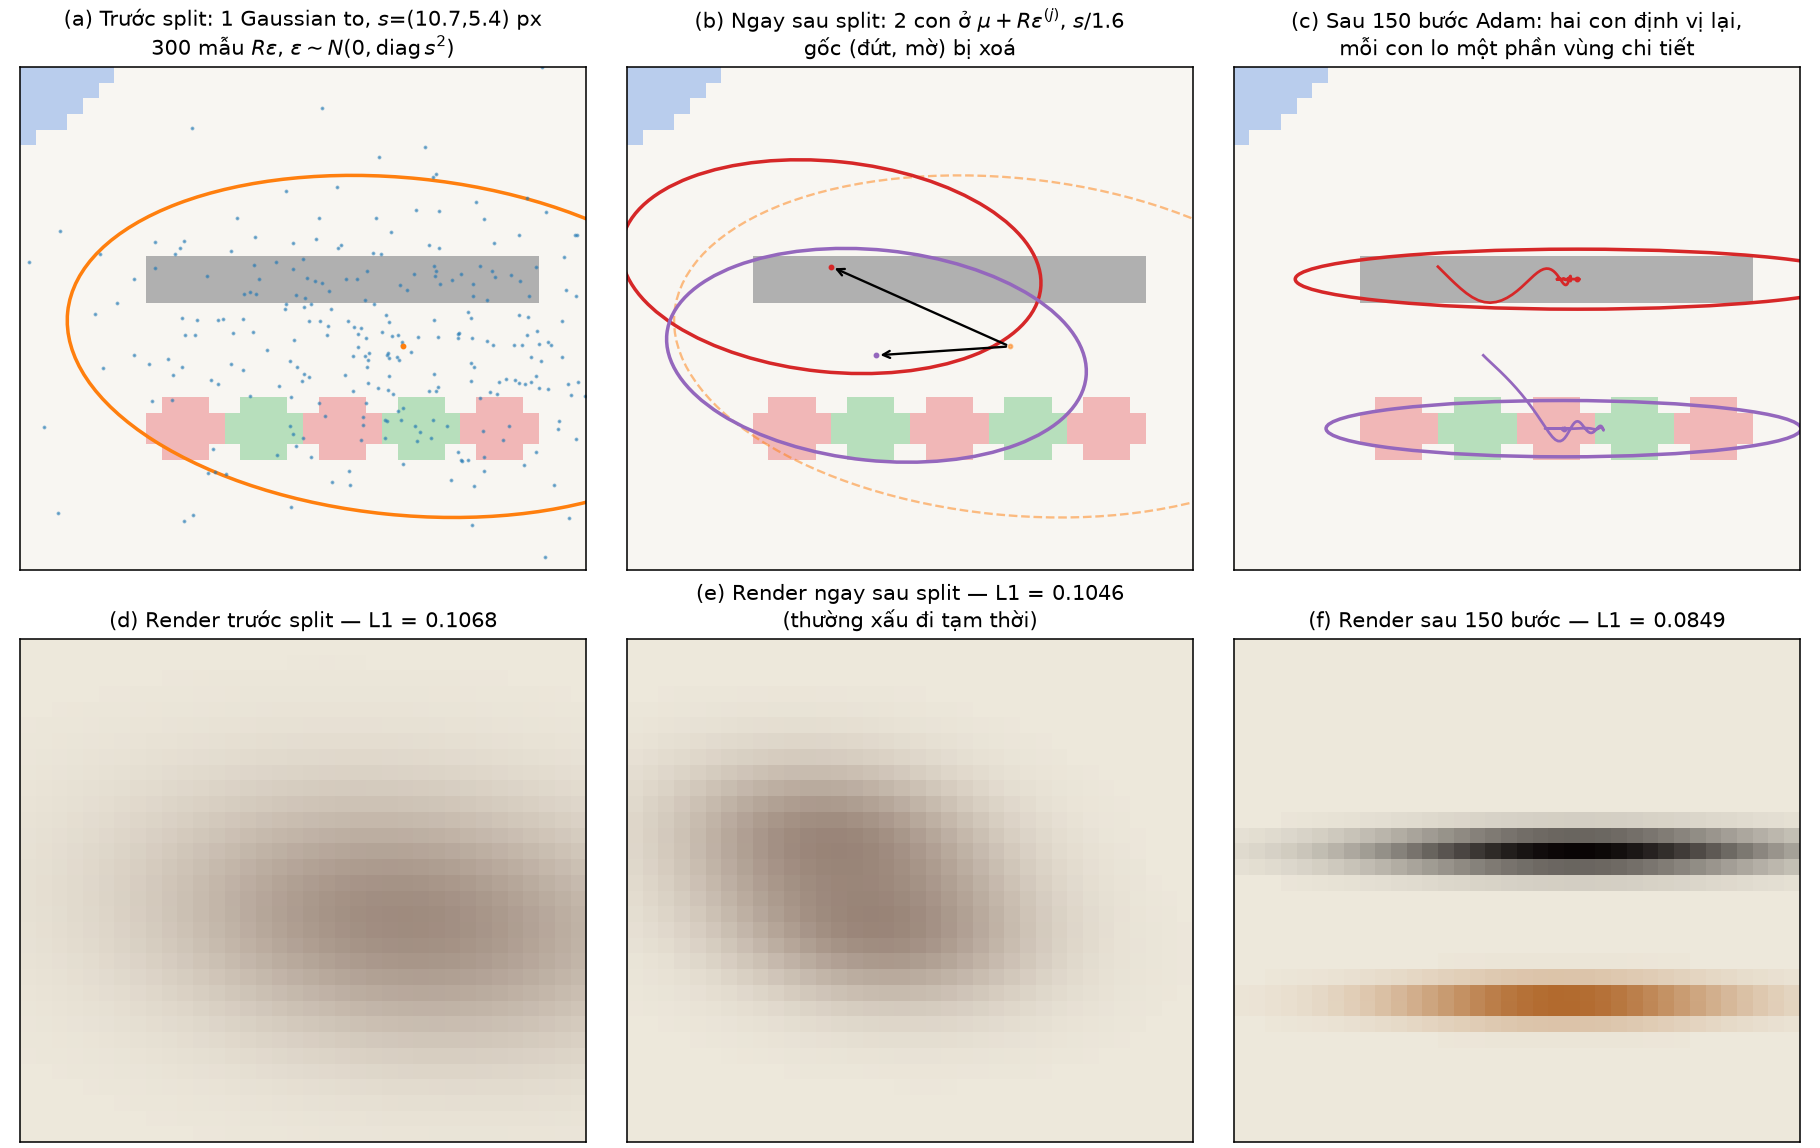
\includegraphics[width=0.95\linewidth]{6_5_split-truoc-sau.png}
\captionof{figure}{\footnotesize Trên: vị trí/hình dạng trước–ngay sau–150 bước sau split. Dưới: render + L1.}
\end{column}
\end{columns}
\end{frame}

% --- 6_6_chuoi-thoi-gian.png ---
\begin{frame}{Chuỗi thời gian: toàn bộ vòng đời densify trên toy model}
\begin{itemize}
    \footnotesize
    \item Khởi tạo kiểu SfM-thu nhỏ: $N_0 = 12$ Gaussian, vị trí lấy mẫu ưu tiên vùng có gradient ảnh mục tiêu lớn (vùng chi tiết).
    \item Huấn luyện $T_{\text{total}}=1200$ vòng bằng Adam; ADC chạy mỗi $K=100$ vòng, trong cửa sổ densify $t\in[100, 900]$.
    \item Các mốc quan sát: $t = 0, 100, 300, 600, 1000$ — tại mỗi mốc ghi lại $N$ và L1 loss.
    \item Qua các mốc, Gaussian tự dịch chuyển, co giãn, nhân đôi (clone/split) và dần phủ kín ảnh mục tiêu, loss giảm liên tục.
\end{itemize}
\begin{center}
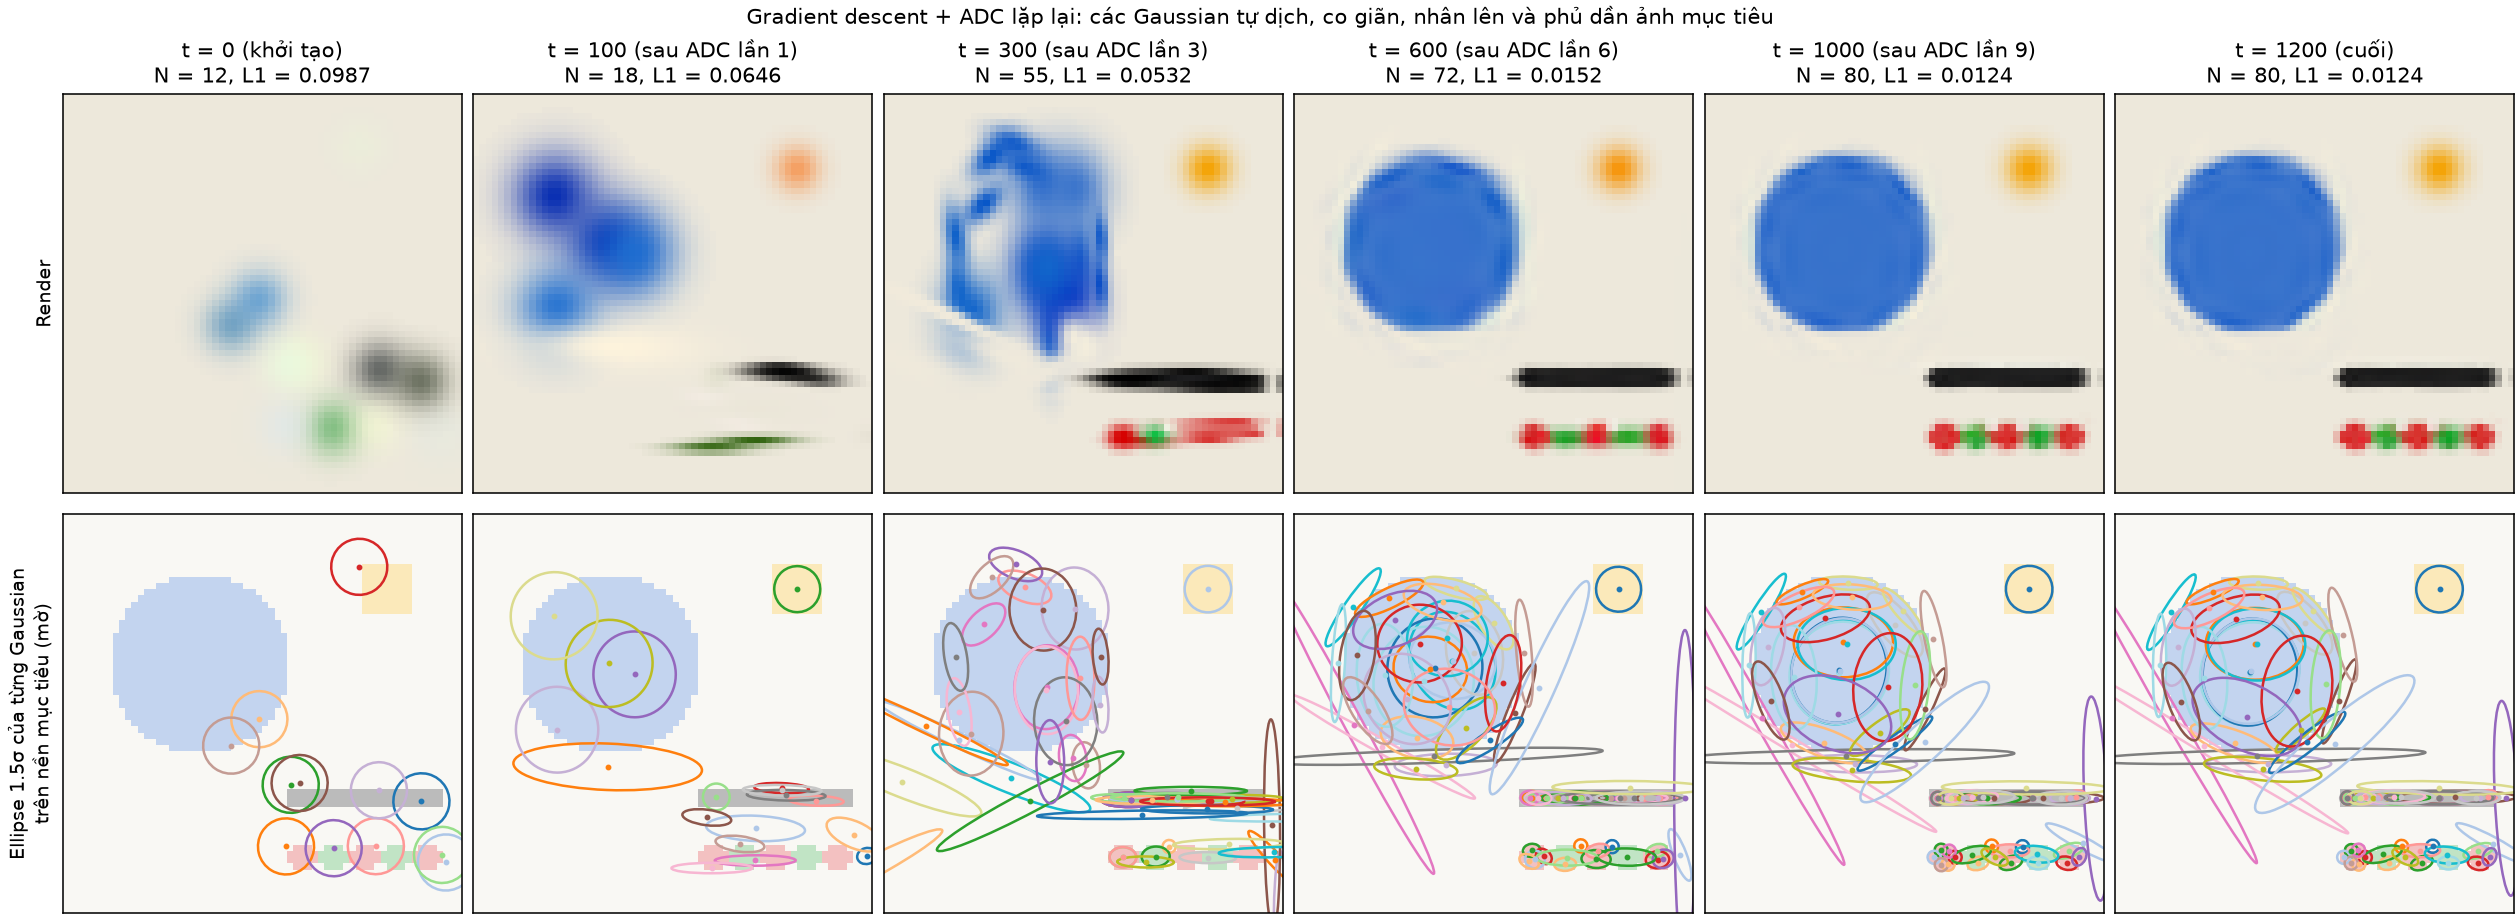
\includegraphics[width=0.85\linewidth]{6_6_chuoi-thoi-gian.png}
\captionof{figure}{\footnotesize Hàng trên: render tại từng mốc thời gian (N và L1 loss). Hàng dưới: ellipse $1.5\sigma$ của từng Gaussian chồng lên ảnh mục tiêu mờ.}
\end{center}
\end{frame}

% --- 6_7_chia-vung.png ---
\begin{frame}{Chia vùng: mỗi Gaussian ``phụ trách'' một lãnh thổ}
\begin{itemize}
    \footnotesize
    \item Với mỗi pixel, xác định Gaussian đóng góp lớn nhất theo trọng số $T_i \alpha_i G_i$ (đóng góp thực sự sau alpha-compositing).
    \item Pixel được tô theo màu của Gaussian ``thắng'' tại đó; màu trắng là nền (khi $T_{\text{end}}$ tại pixel đó lớn hơn mọi đóng góp).
    \item Đường viền đen là biên vật thể mục tiêu (đường mức gradient), dùng để đối chiếu vùng lãnh thổ với hình dạng thật.
    \item Theo thời gian, số lượng lãnh thổ tăng lên (do clone/split) và các lãnh thổ co lại, khớp sát hơn với biên vật thể và vùng chi tiết.
\end{itemize}
\begin{center}
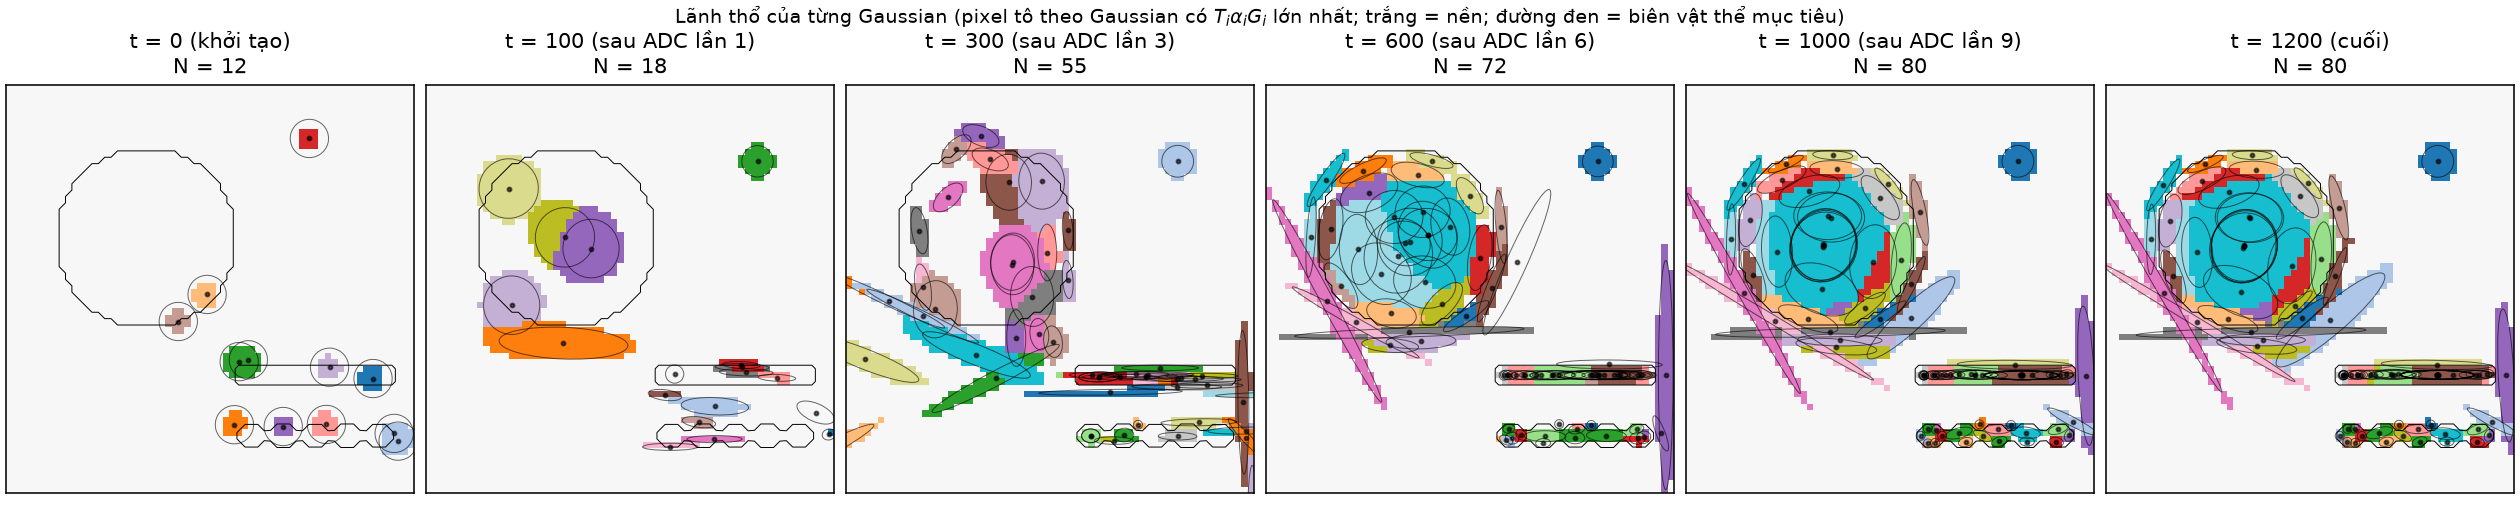
\includegraphics[width=0.85\linewidth]{6_7_chia-vung.png}
\captionof{figure}{\footnotesize Bản đồ lãnh thổ tại các mốc thời gian: pixel tô theo Gaussian có $T_i\alpha_i G_i$ lớn nhất; đường đen = biên vật thể mục tiêu.}
\end{center}
\end{frame}

% --- 6_8_duong-cong-loss-N.png ---
\begin{frame}{Đường cong loss và số Gaussian $N(t)$}
\begin{columns}
\begin{column}{0.5\textwidth}
\begin{itemize}
    \footnotesize
    \item So sánh 3 kịch bản: (i) có ADC; (ii) không ADC, $N$ cố định bằng $N_0$; (iii) không ADC, $N$ cố định bằng $N$ cuối của ADC nhưng khởi tạo ngẫu nhiên ngay từ đầu.
    \item Vạch dọc đánh dấu các mốc ADC (mỗi $K_{\text{ADC}}=100$ vòng).
    \item $N(t)$ tăng theo bậc thang đúng tại các mốc ADC, chỉ trong cửa sổ densify $[100,900]$.
\end{itemize}
\end{column}
\begin{column}{0.5\textwidth}
\begin{itemize}
    \footnotesize
    \item Biểu đồ cột: số Gaussian bị clone / split / prune tại từng mốc ADC — cho thấy tỉ lệ thay đổi giữa các cơ chế qua thời gian.
    \item Có ADC luôn đạt L1 loss thấp hơn rõ rệt so với giữ nguyên $N_0$ ban đầu trong suốt quá trình.
\end{itemize}
\end{column}
\end{columns}
\begin{center}
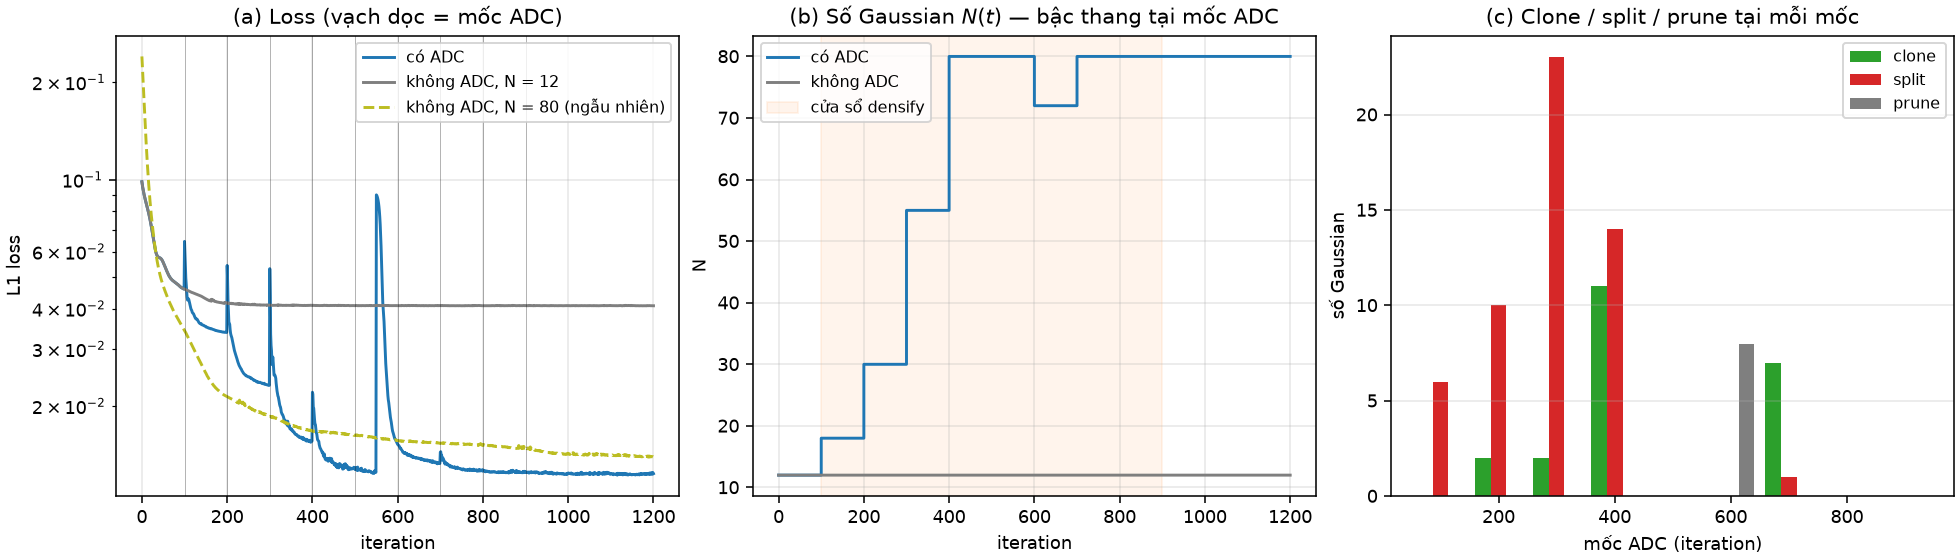
\includegraphics[width=0.95\linewidth]{6_8_duong-cong-loss-N.png}
\captionof{figure}{\footnotesize (a) Loss (thang log, vạch dọc = mốc ADC); (b) $N(t)$ dạng bậc thang; (c) số clone/split/prune tại mỗi mốc ADC.}
\end{center}
\end{frame}

% --- 6_9_kich-thuoc-vs-chi-tiet.png ---
\begin{frame}{Kích thước Gaussian so với mức chi tiết tái tạo}
\begin{itemize}
    \footnotesize
    \item Phân bố kích thước $\max_k s_{i,k}$ (scale lớn nhất mỗi Gaussian) tại $t=0$ so với lúc kết thúc — Gaussian cuối tập trung nhiều hơn quanh và dưới ngưỡng toy $S_{\text{big}}=3.5$ px.
    \item Độ chi tiết vùng phủ của một Gaussian được đo bằng gradient ảnh mục tiêu trung bình trong footprint ($q<9$) của Gaussian đó.
    \item Quan hệ ngược chiều rõ rệt: Gaussian nằm ở vùng chi tiết cao có kích thước nhỏ hơn; Gaussian ở vùng phẳng (ví dụ hình tròn màu đều) có kích thước lớn hơn.
    \item Màu điểm biểu diễn opacity $\alpha$ — hầu hết Gaussian còn lại sau ADC có $\alpha$ cao, phản ánh chúng đóng góp thực chất vào ảnh cuối.
\end{itemize}
\begin{center}
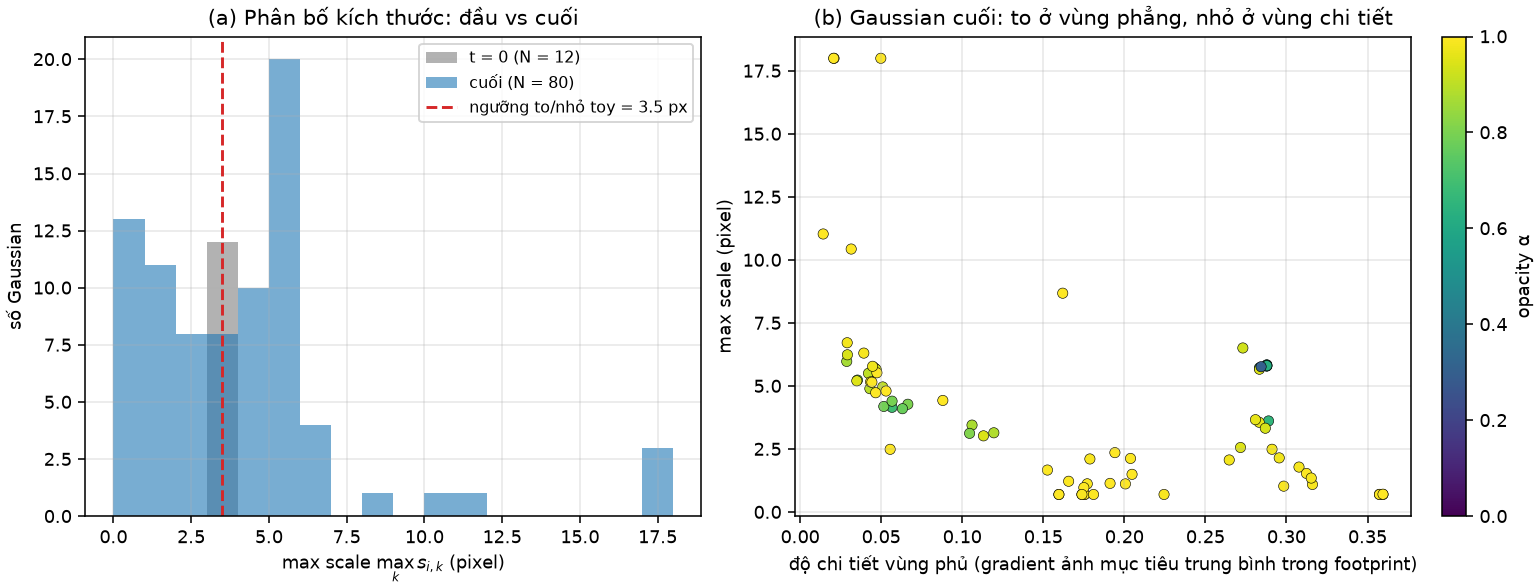
\includegraphics[width=0.8\linewidth]{6_9_kich-thuoc-vs-chi-tiet.png}
\captionof{figure}{\footnotesize (a) Histogram kích thước Gaussian đầu vs cuối, vạch đỏ = ngưỡng $S_{\text{big}}$; (b) scatter độ chi tiết vs kích thước, màu = opacity $\alpha$.}
\end{center}
\end{frame}

% --- 6_10_khong-adc-vs-co-adc.png ---
\begin{frame}{So sánh trực tiếp: không ADC vs có ADC}
\begin{columns}[T]
\begin{column}{0.5\textwidth}
\scriptsize
\begin{itemize}
    \item Ba kịch bản: (1) không ADC, $N{=}N_0$; (2) không ADC, khởi tạo ngẫu nhiên $N{=}N_{\text{cuối}}$; (3) có ADC, $N_0{\to}N_{\text{cuối}}$ dần.
    \item (2) cùng số Gaussian (3) nhưng khởi tạo ngẫu nhiên không khớp tự nhiên vào vùng chi tiết.
    \item[$\Rightarrow$] ADC không chỉ tăng $N$ mà đặt đúng chỗ cần thiết.
\end{itemize}
\end{column}
\begin{column}{0.5\textwidth}
\centering
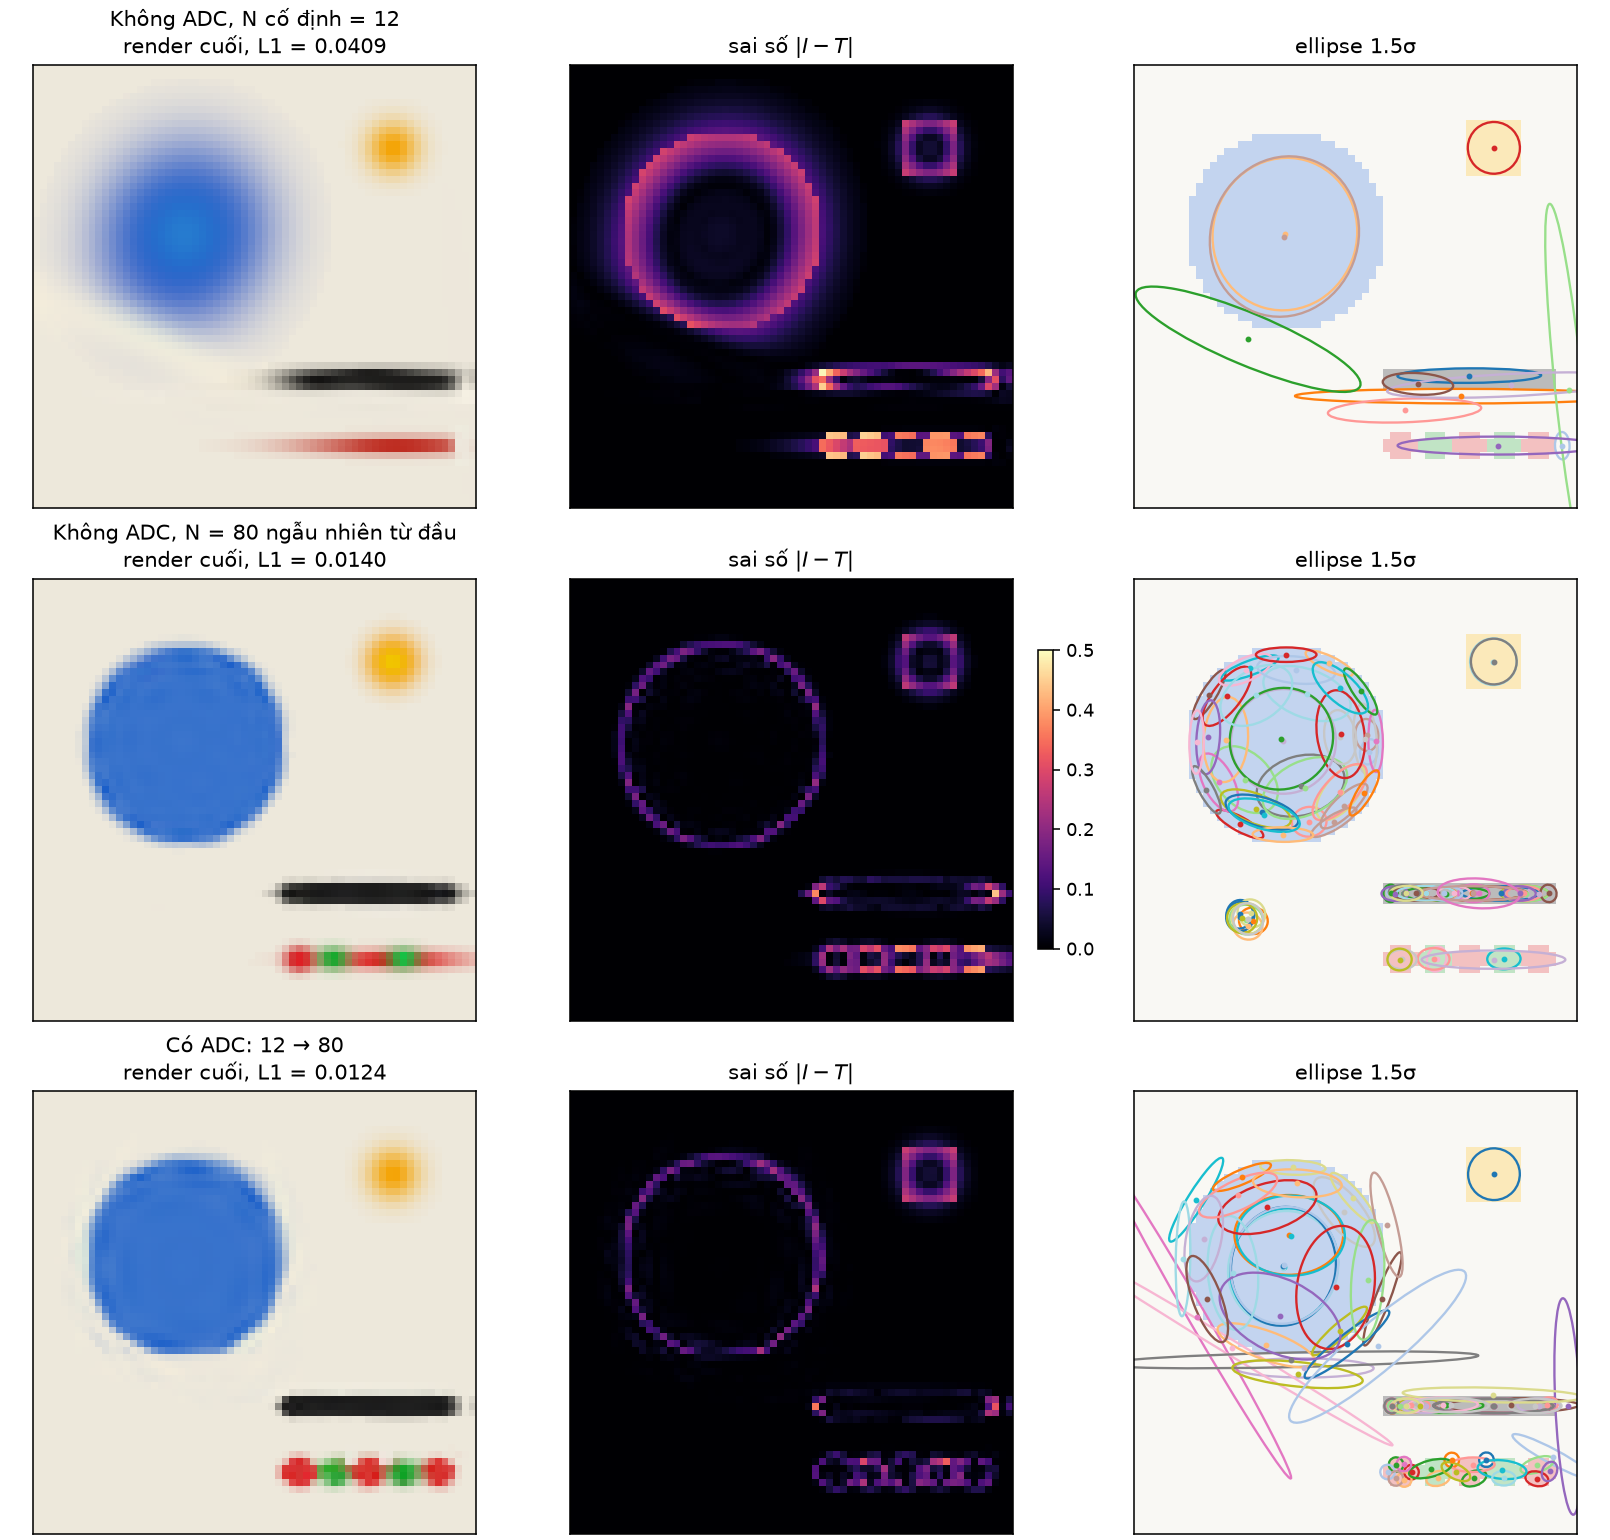
\includegraphics[width=0.85\linewidth]{6_10_khong-adc-vs-co-adc.png}
\captionof{figure}{\footnotesize 3 hàng (không ADC $N_0$; ngẫu nhiên; có ADC) $\times$ 3 cột.}
\end{column}
\end{columns}
\end{frame}

% --- 6_11_prune-opacity.png ---
\begin{frame}{PRUNE: loại bỏ Gaussian dư theo opacity}
\begin{itemize}
    \footnotesize
    \item Tại mốc $t=550$, opacity được reset: $\alpha \leftarrow \min(\alpha,\ \alpha_{\text{reset}}=0.02)$ — buộc mọi Gaussian phải ``chứng minh lại'' sự cần thiết của mình.
    \item Gaussian nào không phục hồi được opacity (không đóng góp giảm loss) sẽ bị đánh dấu để prune tại mốc ADC kế tiếp, theo ngưỡng $\alpha < \varepsilon_{\text{opa}} = 0.03$.
    \item So sánh render ngay trước và ngay sau prune: sai lệch tối đa $\max|\Delta I|$ rất nhỏ — ảnh gần như không đổi dù đã loại bỏ các Gaussian dư.
    \item Kết quả: mô hình gọn hơn (ít Gaussian hơn) mà chất lượng tái tạo giữ nguyên — đúng vai trò dọn dẹp của bước prune trong chu trình ADC.
\end{itemize}
\begin{center}
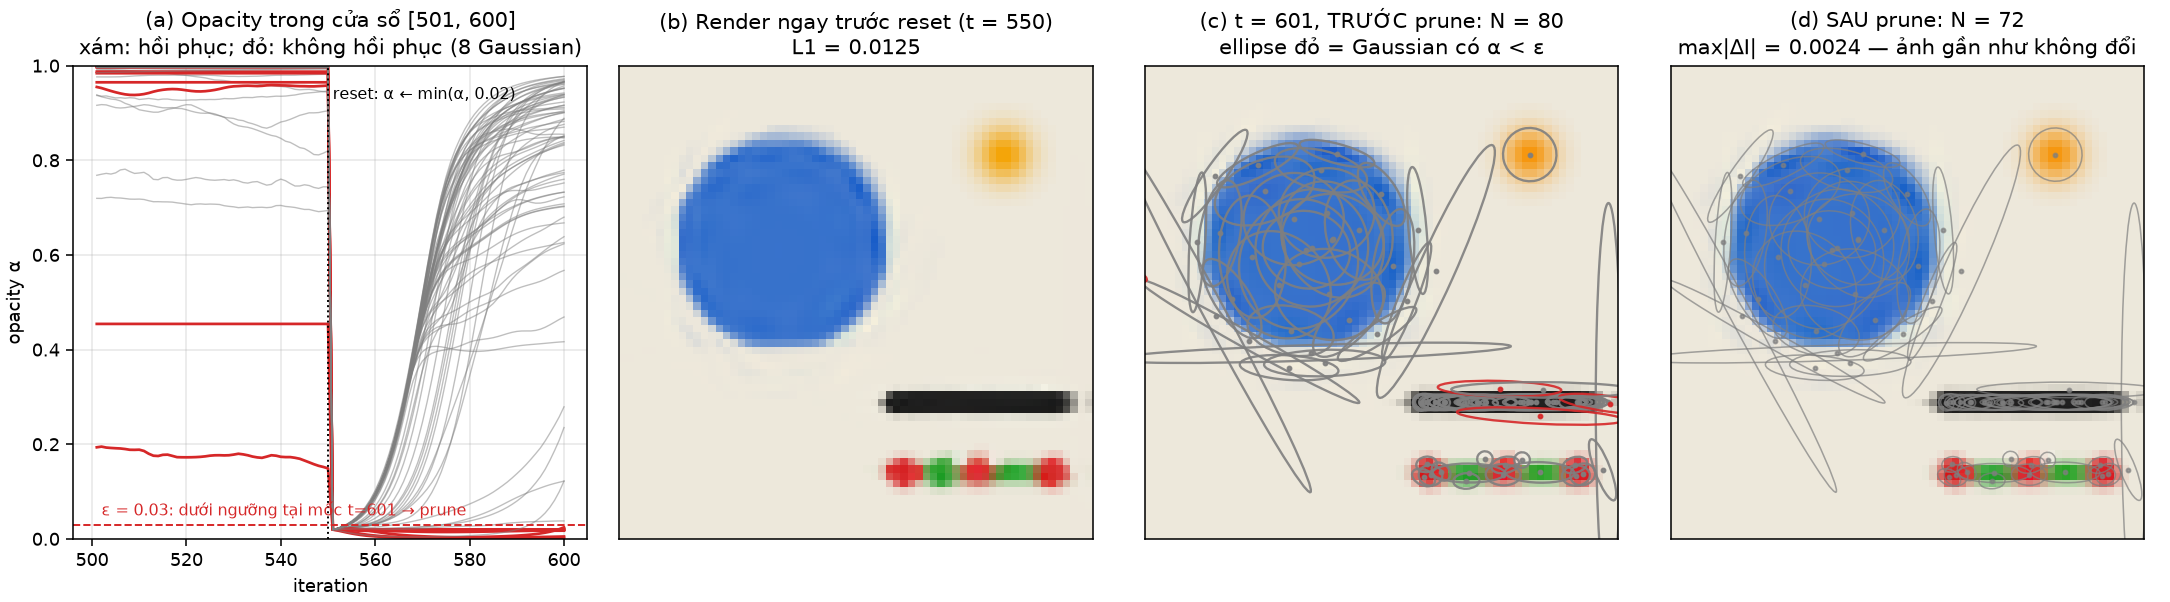
\includegraphics[width=0.8\linewidth]{6_11_prune-opacity.png}
\captionof{figure}{\footnotesize (a) Quỹ đạo opacity quanh mốc reset (đỏ = bị prune); (b) render ngay trước reset; (c) trước prune, ellipse đỏ = $\alpha<\varepsilon$; (d) sau prune — ảnh gần như không đổi.}
\end{center}
\end{frame}


\section{ADC chuyên sâu — P7: So sánh cuối 3DGS vs FastGS}
% partADC_7.tex — Phần 7 (chương ADC): so sánh toàn pipeline 3DGS gốc vs FastGS-lite trên toy model
% Chỉ chứa các khối frame, không có preamble. Include từ main.tex.

% --- 7_1_3dgs-chuoi-thoi-gian.png ---
\begin{frame}{Chuỗi thời gian ADC: 3DGS gốc trên toy 2D}
\begin{columns}[T]
\begin{column}{0.45\linewidth}
\footnotesize
\begin{itemize}
  \item ADC của \textbf{3DGS gốc} (Kerbl 2023) chỉ dùng gradient vị trí trung bình tích luỹ $\bar g$, \textbf{có dấu}:
  \[
    \text{clone} = [\|\bar g\| \ge \tau] \wedge [\max s \le S_{\text{BIG}}]
  \]
  \[
    \text{split} = [\|\bar g\| \ge \tau] \wedge [\max s > S_{\text{BIG}}]
  \]
  \item Prune: xoá \textbf{ngay lập tức} mọi Gaussian có $\alpha < \varepsilon_{\text{opa}}$ (hoặc $\max s > S_{\text{HUGE}}$ sau mốc reset $\alpha$).
  \item \textbf{Không} có: trần opacity, Importance đa view, prune multinomial, hay final prune.
  \item Hình vẽ: render (hàng trên) và ellipse $1.5\sigma$ của từng Gaussian trên nền mục tiêu mờ (hàng dưới), tại 6 mốc snapshot $t \in \{0, 100, 300, 600, 1000, T_{\text{total}}\}$, cùng $N$ và $L_1$ mỗi mốc.
\end{itemize}
\end{column}
\begin{column}{0.55\linewidth}
\centering
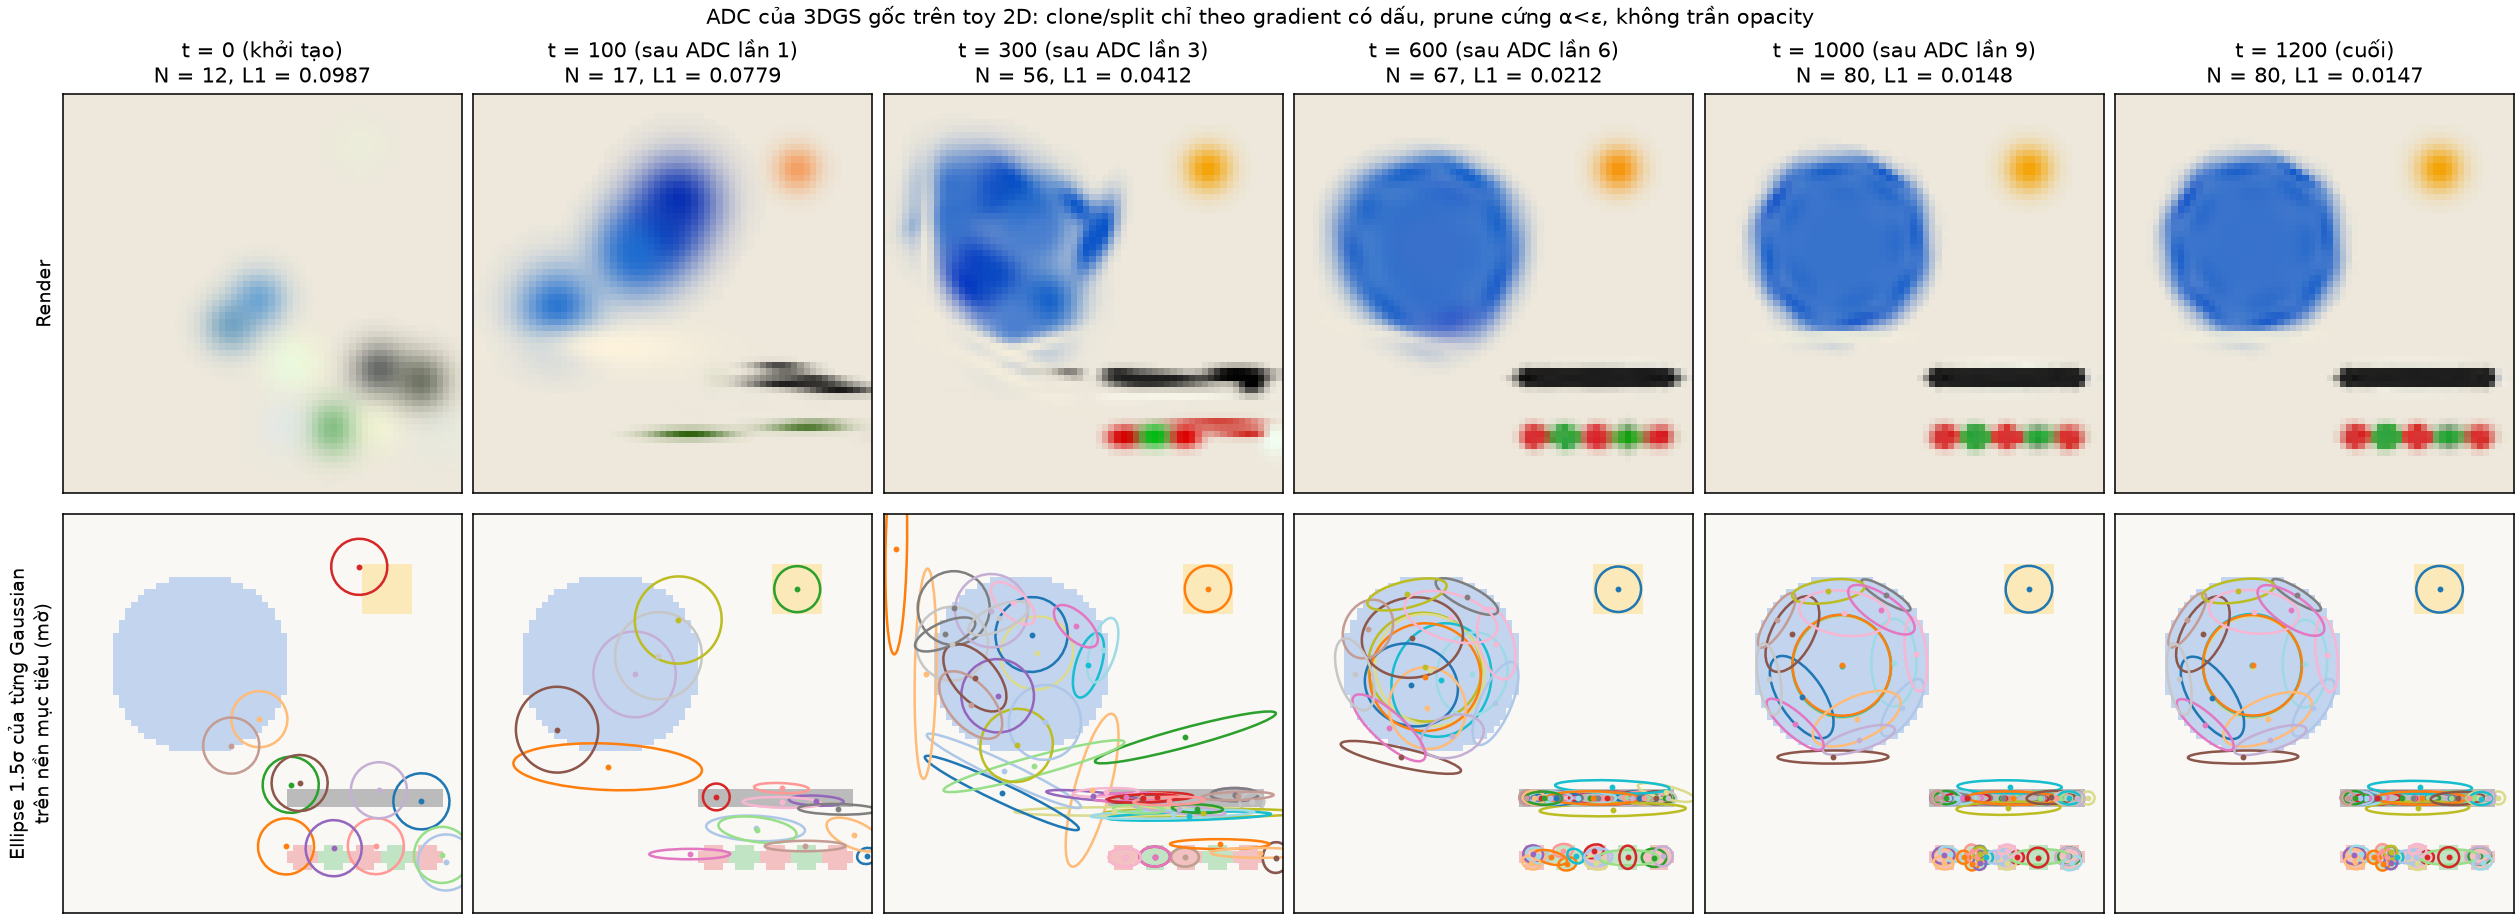
\includegraphics[width=0.95\linewidth]{7_1_3dgs-chuoi-thoi-gian.png}
\captionof{figure}{\footnotesize ADC của 3DGS gốc trên toy 2D: clone/split chỉ theo gradient có dấu, prune cứng $\alpha<\varepsilon$, không trần opacity.}
\end{column}
\end{columns}
\end{frame}

% --- 7_2_fastgs-chuoi-thoi-gian.png ---
\begin{frame}{Chuỗi thời gian ADC: FastGS-lite trên CÙNG toy model}
\begin{columns}[T]
\begin{column}{0.45\linewidth}
\footnotesize
\begin{itemize}
  \item Cùng seed, cùng layout với 3DGS gốc, nhưng FastGS-lite thêm \textbf{Importance đa view} ($V=1$ view trong toy) và gradient \textbf{tuyệt đối}:
  \[
    \text{clone} = [\|\bar g\| \ge \tau] \wedge [\max s \le S_{\text{BIG}}] \wedge [\text{Imp} > \text{IMP\_THR}]
  \]
  \[
    \text{split} = [\|\bar g_{\text{abs}}\| \ge \tau_{\text{abs}}] \wedge [\max s > S_{\text{BIG}}] \wedge [\text{Imp} > \text{IMP\_THR}]
  \]
  \item Prune: lập tập ứng viên $C = \{\alpha < \varepsilon_{\text{opa}} \vee \max s > S_{\text{HUGE}}\}$, trọng số $w_i = 1/(10^{-6} + 1 - \text{Pruning}_i)$, rút mẫu $S \sim \text{Multinomial}(w, \lfloor 0.5|C|\rfloor)$ không hoàn lại, xoá $C \cap S$.
  \item Sau mỗi ADC: trần opacity $\alpha \leftarrow \min(\alpha, 0.8)$.
  \item Final prune bổ sung tại $t = 1000, 1100$.
\end{itemize}
\end{column}
\begin{column}{0.55\linewidth}
\centering
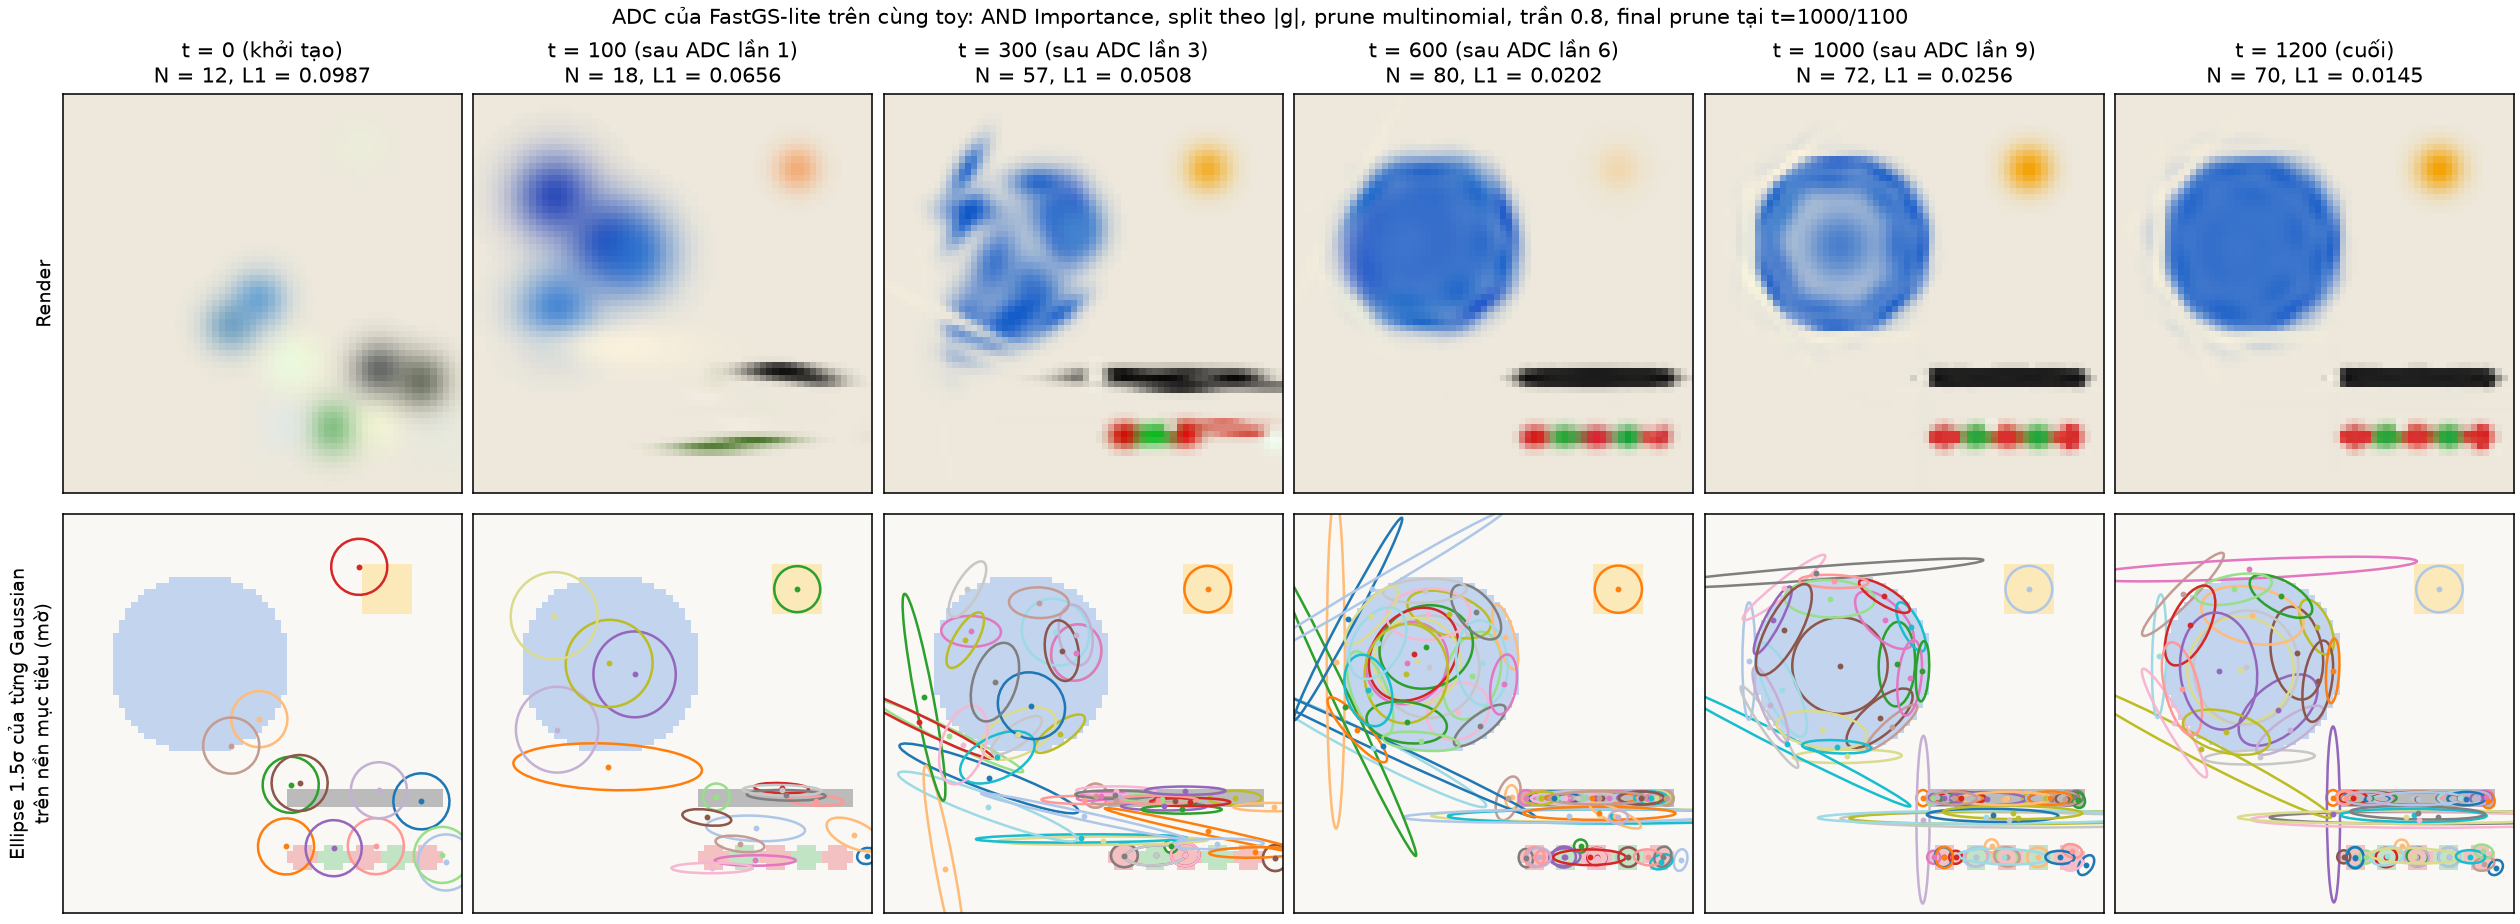
\includegraphics[width=0.95\linewidth]{7_2_fastgs-chuoi-thoi-gian.png}
\captionof{figure}{\footnotesize ADC của FastGS-lite trên cùng toy: AND với Importance, split theo $|g|$, prune multinomial, trần 0.8, final prune tại $t=1000/1100$.}
\end{column}
\end{columns}
\end{frame}

% --- 7_3_chia-vung-3dgs-vs-fastgs.png ---
\begin{frame}{Bản đồ lãnh thổ: 3DGS gốc vs FastGS-lite}
\footnotesize
\begin{itemize}
  \item Mỗi pixel được tô theo Gaussian có $T_i \alpha_i G_i$ lớn nhất tại pixel đó (lãnh thổ chiếm ưu thế trong alpha-blend) — trắng = nền, đường đen = biên vật thể mục tiêu.
  \item So sánh trực tiếp 2 hàng $\times$ 6 mốc thời gian $t \in \{0, 100, 300, 600, 1000, T_{\text{total}}\}$: hàng trên = 3DGS gốc, hàng dưới = FastGS-lite.
  \item Vì clone/split của FastGS bị chặn thêm bởi điều kiện Importance và dùng gradient tuyệt đối cho split, ranh giới các mảng lãnh thổ (đặc biệt tại vùng biên vật thể) tách rời rõ rệt so với 3DGS gốc.
  \item Đây là bằng chứng trực quan cho thấy hai bộ luật ADC khác nhau dẫn đến \textbf{cấu trúc không gian tham số khác nhau}, không chỉ khác về $N$ hay loss.
\end{itemize}
\centering
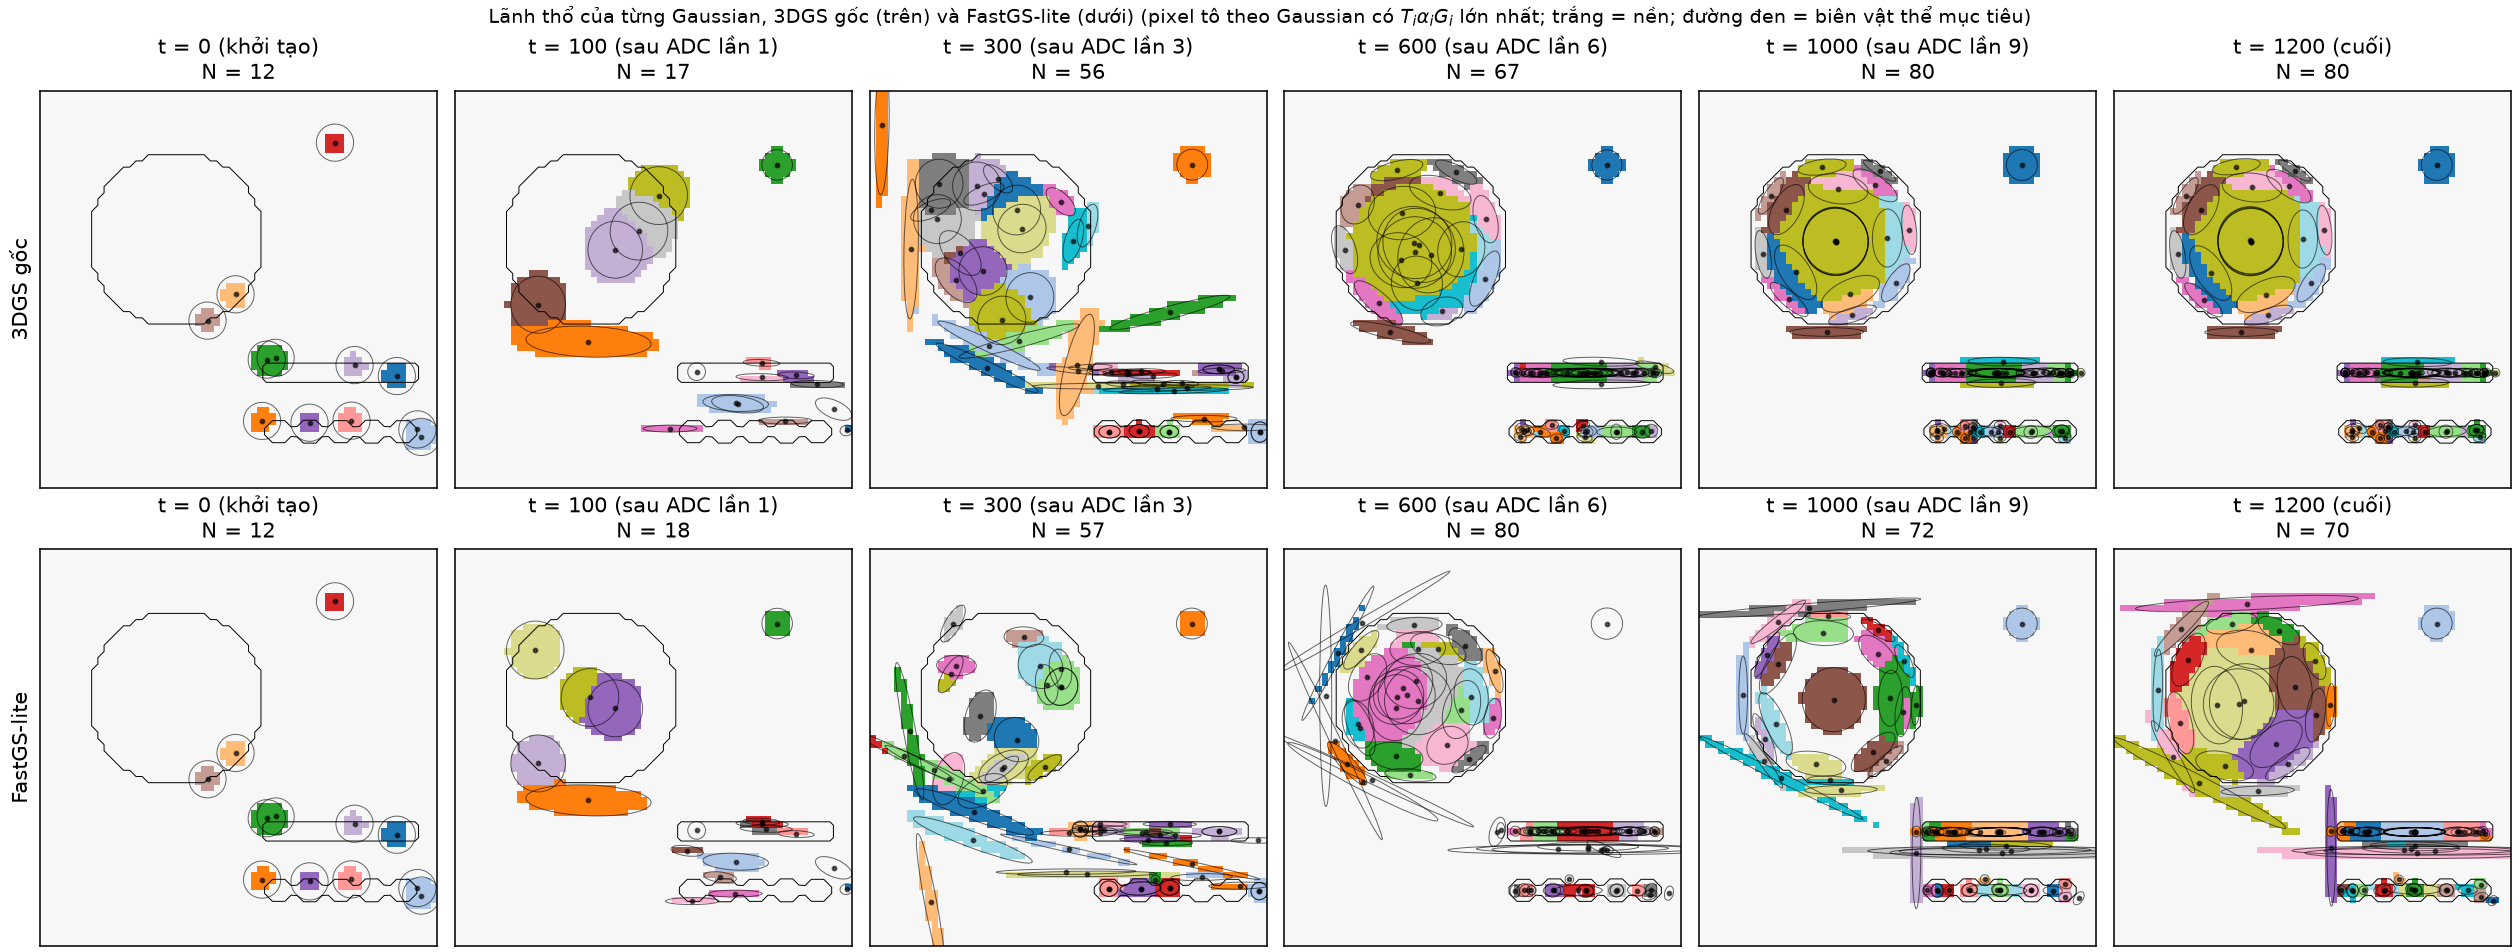
\includegraphics[width=0.7\linewidth]{7_3_chia-vung-3dgs-vs-fastgs.png}
\captionof{figure}{\footnotesize Lãnh thổ của từng Gaussian, 3DGS gốc (trên) và FastGS-lite (dưới), 6 mốc thời gian.}
\end{frame}

% --- 7_4_loss-N-clone-split-prune.png ---
\begin{frame}{Loss, $N(t)$ và các sự kiện clone/split/prune}
\footnotesize
\begin{itemize}
  \item \textbf{(a)} Loss $L_1$ theo thời gian (thang log) cho 3 kịch bản: ADC 3DGS gốc, ADC FastGS-lite, và không dùng ADC ($N$ cố định) — các vạch mờ đánh dấu mốc ADC, vạch tím đứt đánh dấu mốc reset $\alpha$, vạch xanh đứt đánh dấu final prune của FastGS.
  \item \textbf{(b)} Số Gaussian $N(t)$: FastGS-lite kết thúc với $N$ \textbf{ít hơn} 3DGS gốc nhờ prune multinomial và final prune (mũi tên chú thích "final prune $-n_r$" tại từng mốc $t \in$ FINAL\_AT); trần $N = N_{\text{MAX}}$ (toy) được vẽ nét đứt.
  \item \textbf{(c)} Số Gaussian clone/split/prune tại mỗi mốc ADC, 3DGS gốc (gạch chéo) cạnh FastGS-lite (đặc) — cột riêng biệt cho final prune của FastGS.
  \item Liên hệ nhân-quả trực tiếp: mỗi bước nhảy của $N(t)$ ở (b) khớp với sự kiện clone/split/prune ở (c), và mỗi lần $N$ thay đổi kéo theo bước ngoặt trên đường loss ở (a).
\end{itemize}
\centering
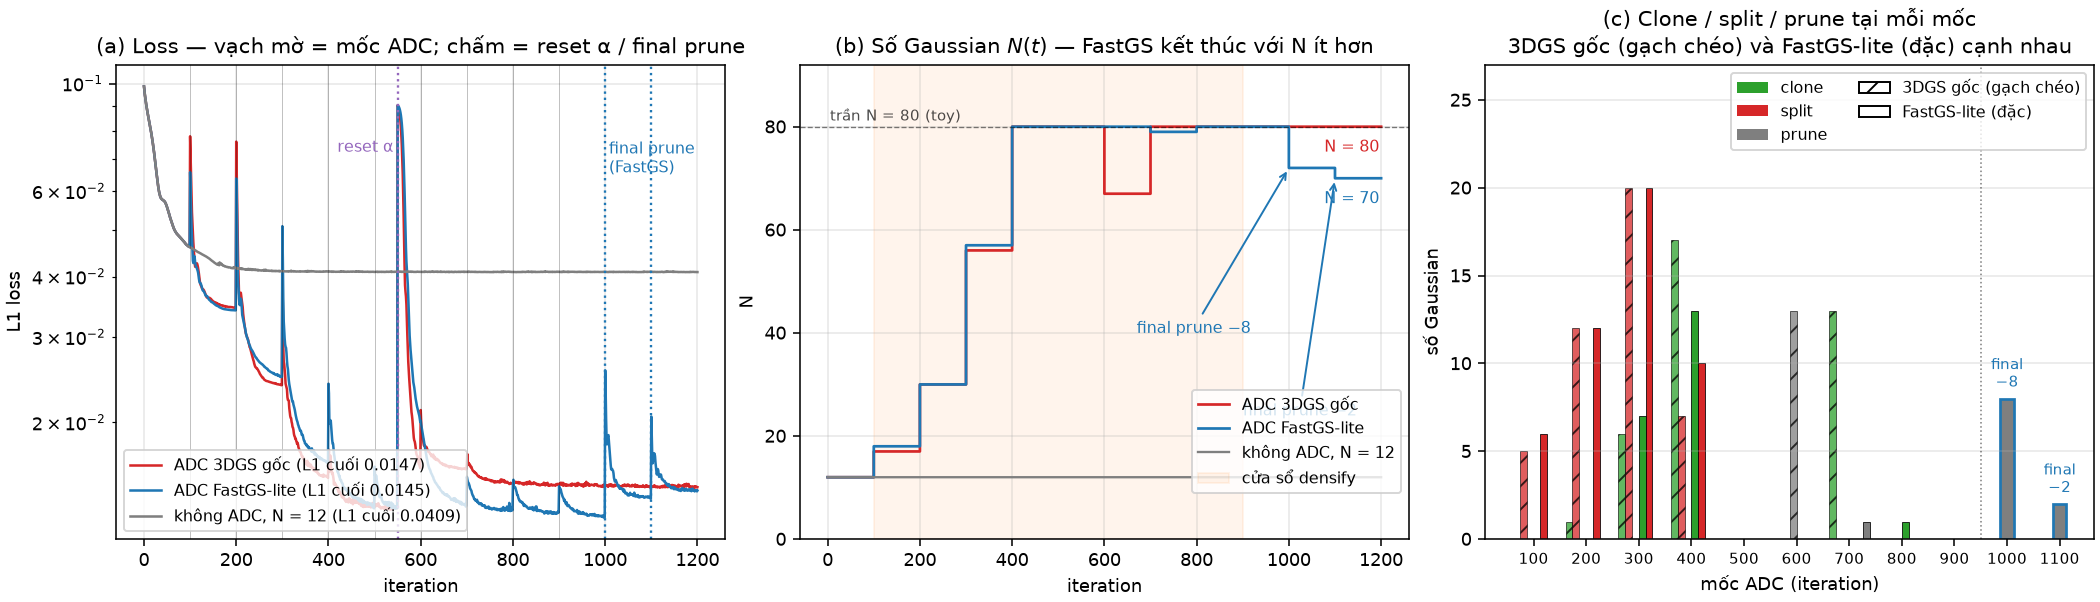
\includegraphics[width=0.85\linewidth]{7_4_loss-N-clone-split-prune.png}
\captionof{figure}{\footnotesize Loss, $N(t)$, và clone/split/prune theo mốc — 3DGS gốc vs FastGS-lite vs không ADC.}
\end{frame}

% --- 7_5_cuoi-3dgs-fastgs-khong-adc.png ---
\begin{frame}{Kết quả render cuối cùng: 3 kịch bản đối chiếu}
\scriptsize
\begin{itemize}
  \item Hàng 1 — \textbf{ADC 3DGS gốc}: $N$ tăng từ khởi tạo lên $N$ cuối, $L_1$ cuối như trong hình.
  \item Hàng 2 — \textbf{ADC FastGS-lite}: $L_1$ cuối \textbf{tương đương} nhưng \textbf{ít Gaussian hơn} — hiệu quả của Importance + prune multinomial + final prune.
  \item Hàng 3 — \textbf{Không ADC}: $N{=}N_0$ cố định, không clone/split/prune — chất lượng kém hơn rõ rệt.
  \item Mỗi hàng: render cuối, sai số $|I-T|$, ellipse $1.5\sigma$. Viền màu: đỏ=3DGS, xanh=FastGS, xám=không ADC.
\end{itemize}
\centering
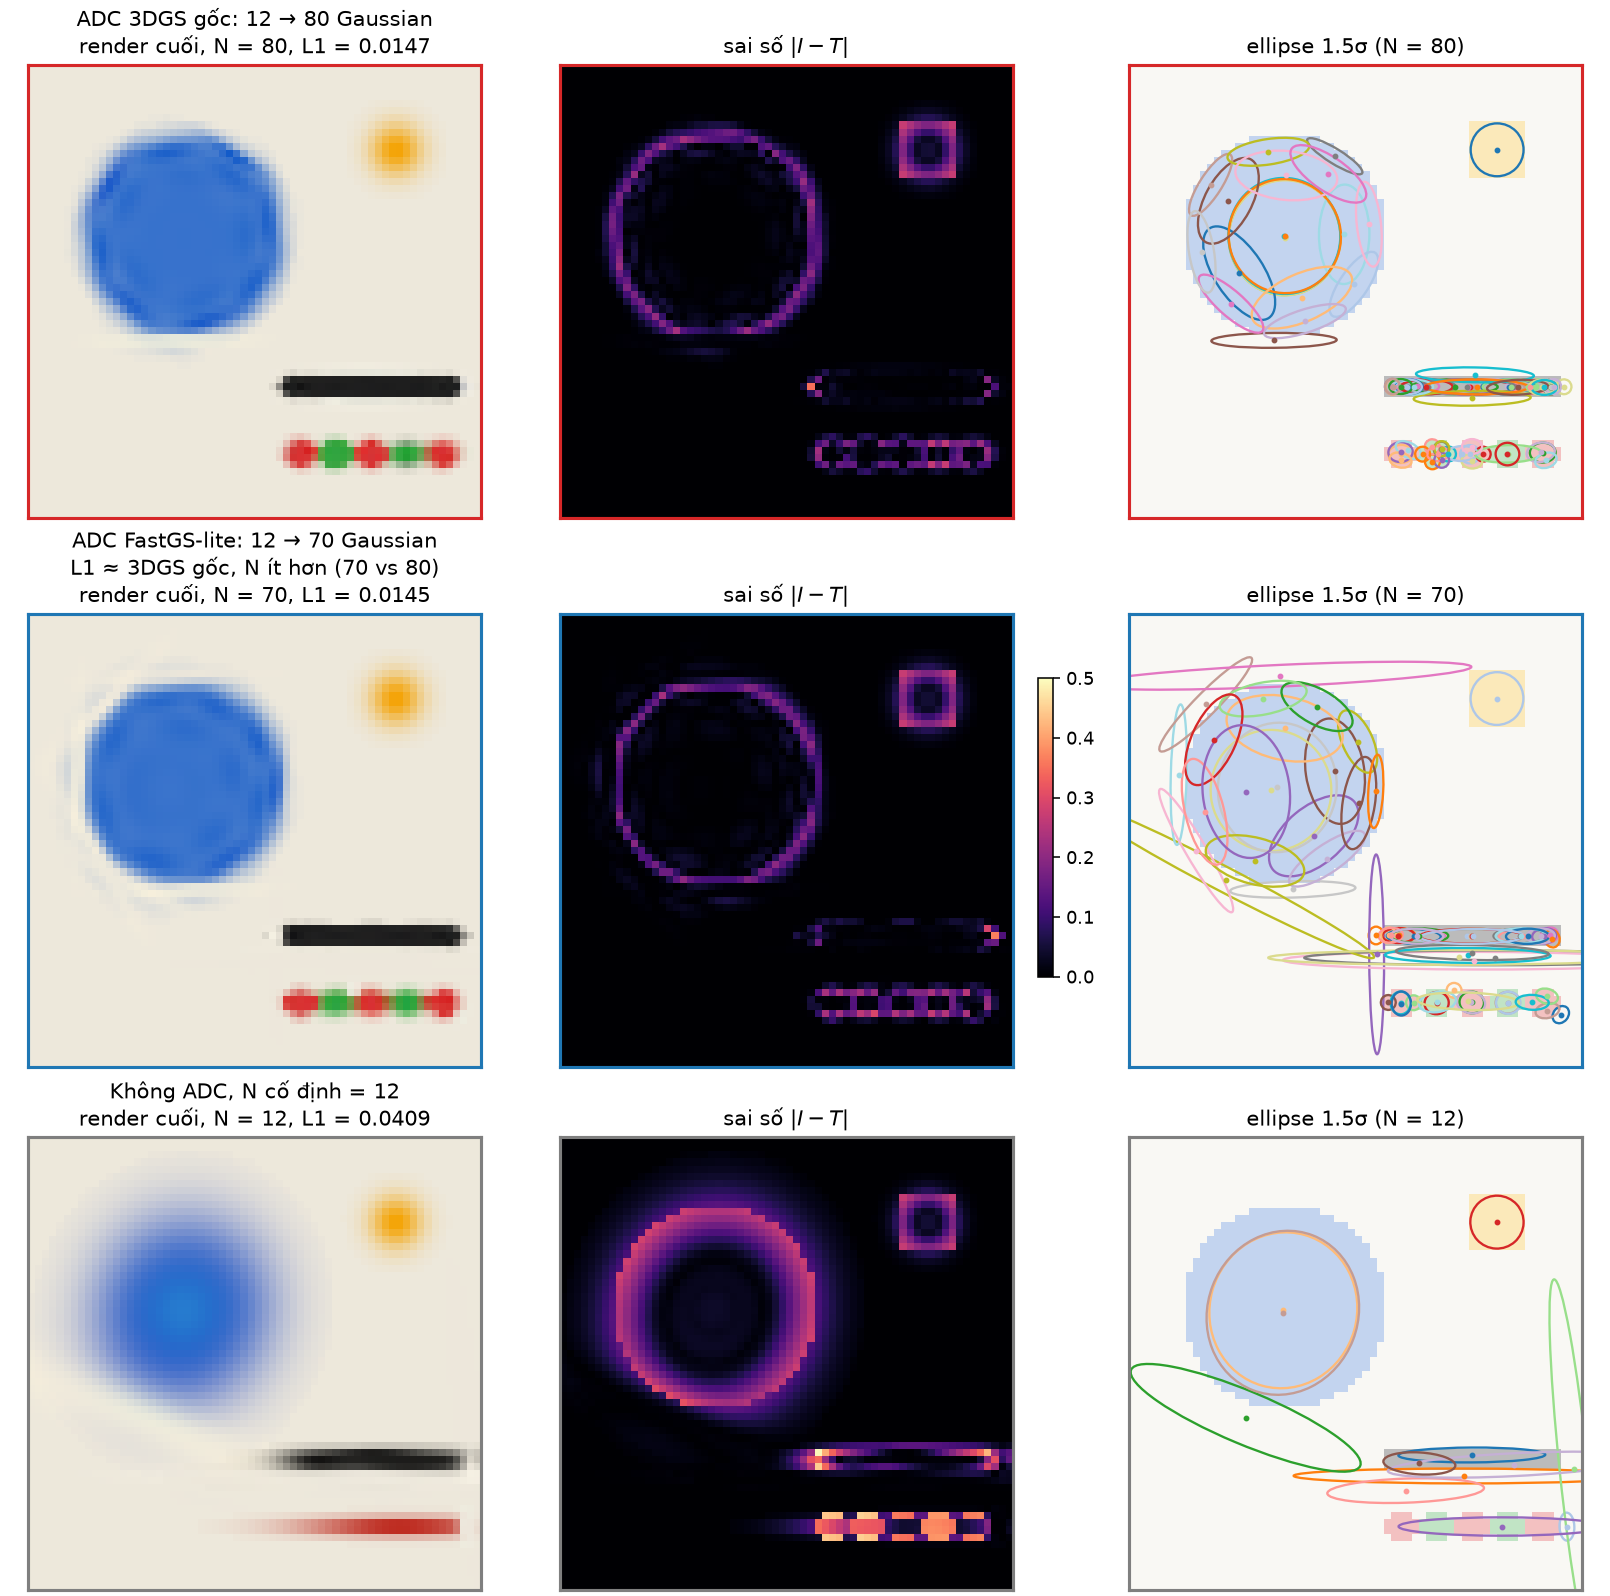
\includegraphics[width=0.42\linewidth]{7_5_cuoi-3dgs-fastgs-khong-adc.png}
\captionof{figure}{\footnotesize Đối chiếu cuối: ADC 3DGS gốc / ADC FastGS-lite / không ADC.}
\end{frame}

% --- 7_6_and-importance-tren-toy.png ---
\begin{frame}{Cải tiến 1: logic AND với Importance, số liệu thật trên toy}
\begin{columns}[T]
\begin{column}{0.48\linewidth}
\footnotesize
\begin{itemize}
  \item Nhắc lại Phần 4: FastGS chỉ densify khi \textbf{cả} gradient \textbf{và} Importance đa view đều vượt ngưỡng — ở đây minh hoạ cụ thể bằng số liệu tại một mốc $t$ chọn từ log thật (ưu tiên $t=300$, hoặc mốc có nhiều Gaussian bị chặn nhất).
  \item Mặt nạ lỗi (bước \textcircled{1}\textcircled{2}\textcircled{3}): $\hat e(x) = \text{minmax}(\text{mean}_{\text{ch}}|I - T|) > 0.1$.
  \item Importance$_i$ = số pixel lỗi trong footprint hữu hình của Gaussian $i$ (đã qua 3 cửa lọc: $3\sigma$, $w \ge 1/255$, $T \ge 10^{-4}$); ngưỡng $\text{IMP\_THR} = 5$.
  \item 4 nhóm quyết định: densify ở \textbf{cả hai} phương pháp (xanh lá), 3DGS muốn densify nhưng FastGS \textbf{chặn} vì $\text{Imp} \le 5$ (đỏ, dấu X — gradient "muốn đổi" nhưng render không thật sự sai), chỉ FastGS densify nhờ split theo $|g|$ (cam), và không ai densify (xám).
\end{itemize}
\end{column}
\begin{column}{0.52\linewidth}
\centering
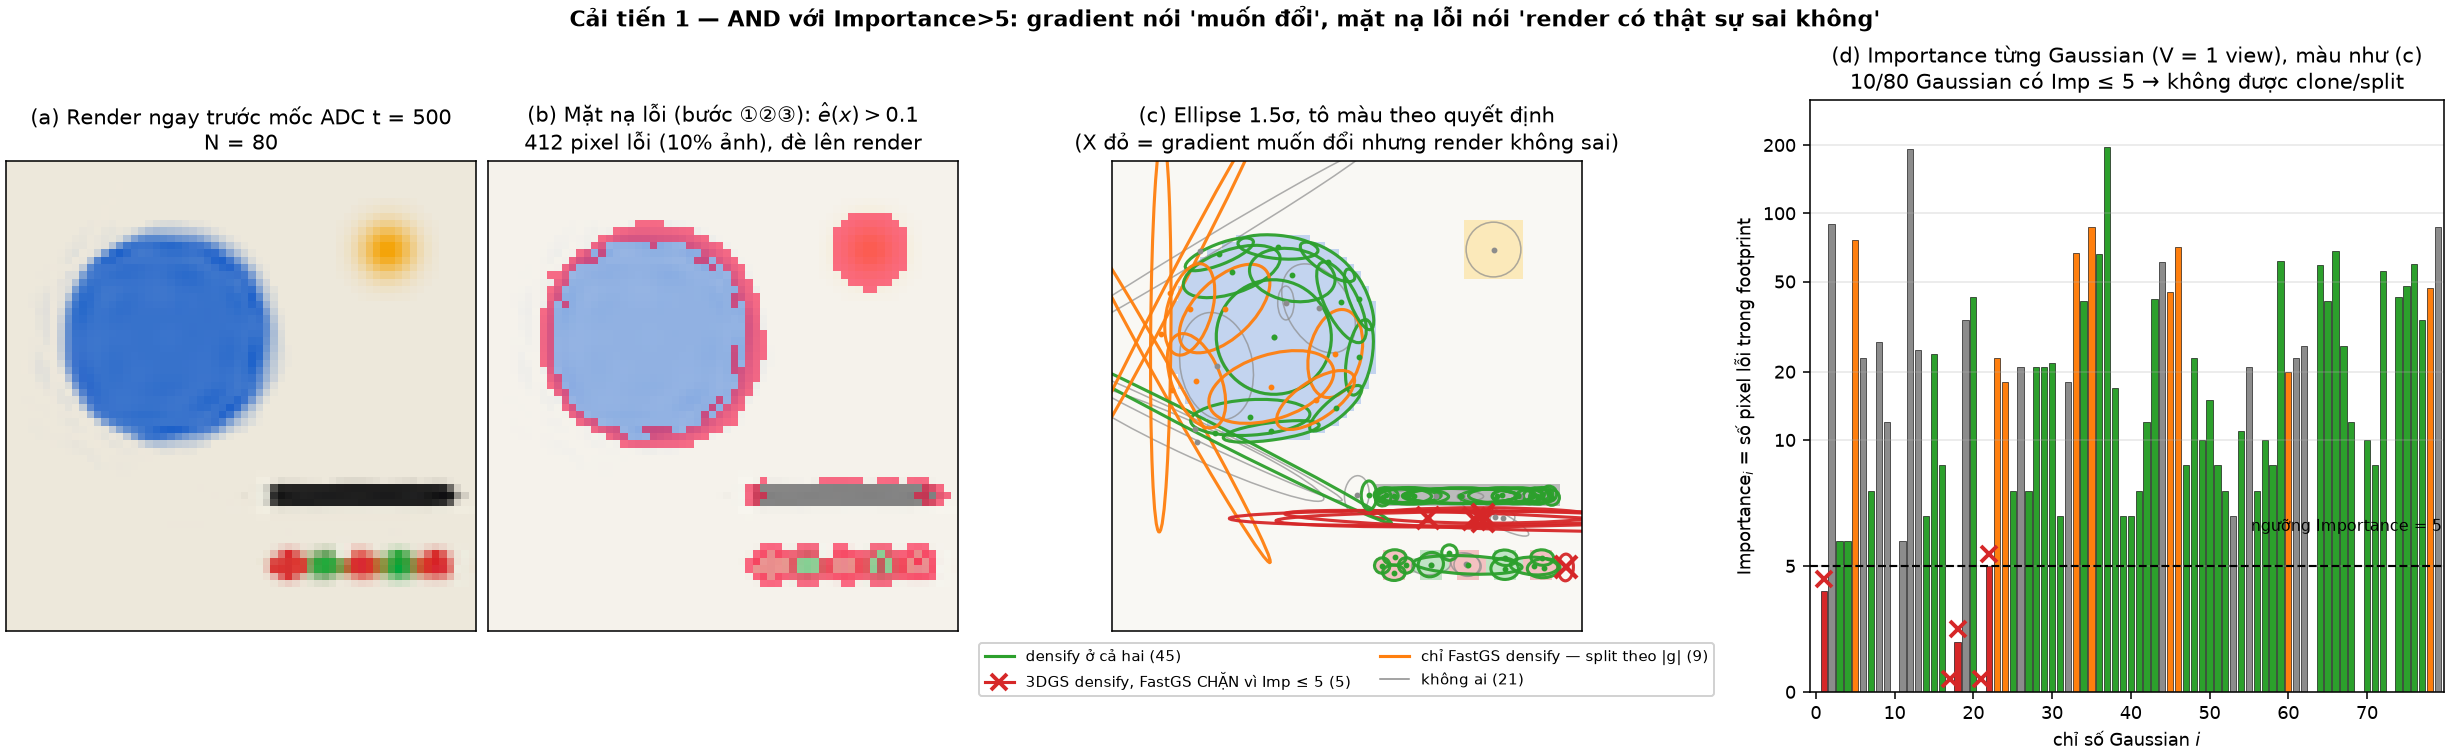
\includegraphics[width=\linewidth]{7_6_and-importance-tren-toy.png}
\captionof{figure}{\footnotesize Cải tiến 1 — AND với Importance$>5$: gradient nói "muốn đổi", mặt nạ lỗi nói "render có thật sự sai không".}
\end{column}
\end{columns}
\end{frame}

% --- 7_7_abs-vs-signed-split.png ---
\begin{frame}{Cải tiến 2: split theo $\sum|g|$ thay vì $\sum g$ (có dấu)}
\footnotesize
\begin{itemize}
  \item Vấn đề của gradient \textbf{có dấu}: các gradient pixel trong footprint của một Gaussian to có thể kéo về nhiều phía khác nhau trong cùng một ảnh, \textbf{triệt tiêu lẫn nhau} khi cộng vector.
  \item Chọn Gaussian $i^*$ minh hoạ: tại mốc $t$, $\|\sum_x g_x\|$ (có dấu) rất nhỏ so với $\sum_x |g_x|$ (tuyệt đối) — tỉ lệ chênh lệch thể hiện trực tiếp trên hình (ví dụ "gấp $k$ lần").
  \item Tích luỹ theo thời gian: $\|\bar g\|/\tau < 1 \Rightarrow$ 3DGS \textbf{bỏ qua} $i^*$; nhưng $\|\bar g_{\text{abs}}\|/\tau_{\text{abs}} \ge 1 \Rightarrow$ FastGS \textbf{split} $i^*$.
  \item So sánh kết quả sau $N_{\text{ADAM}} = 80$ bước Adam: \textbf{không split} (như 3DGS, $L_1$ cải thiện ít) vs \textbf{split} $i^*$ thành 2 con (FastGS, $L_1$ giảm ngay sau split rồi tiếp tục giảm qua 80 bước Adam).
  \item Panel (b): bar so sánh $\|\bar g\|$ (có dấu, 3DGS) vs $\|\bar g_{\text{abs}}\|$ (FastGS) cho toàn bộ Gaussian to ($\max s > S_{\text{BIG}}$), có đường ngưỡng $\tau$ và $\tau_{\text{abs}}$.
\end{itemize}
\centering
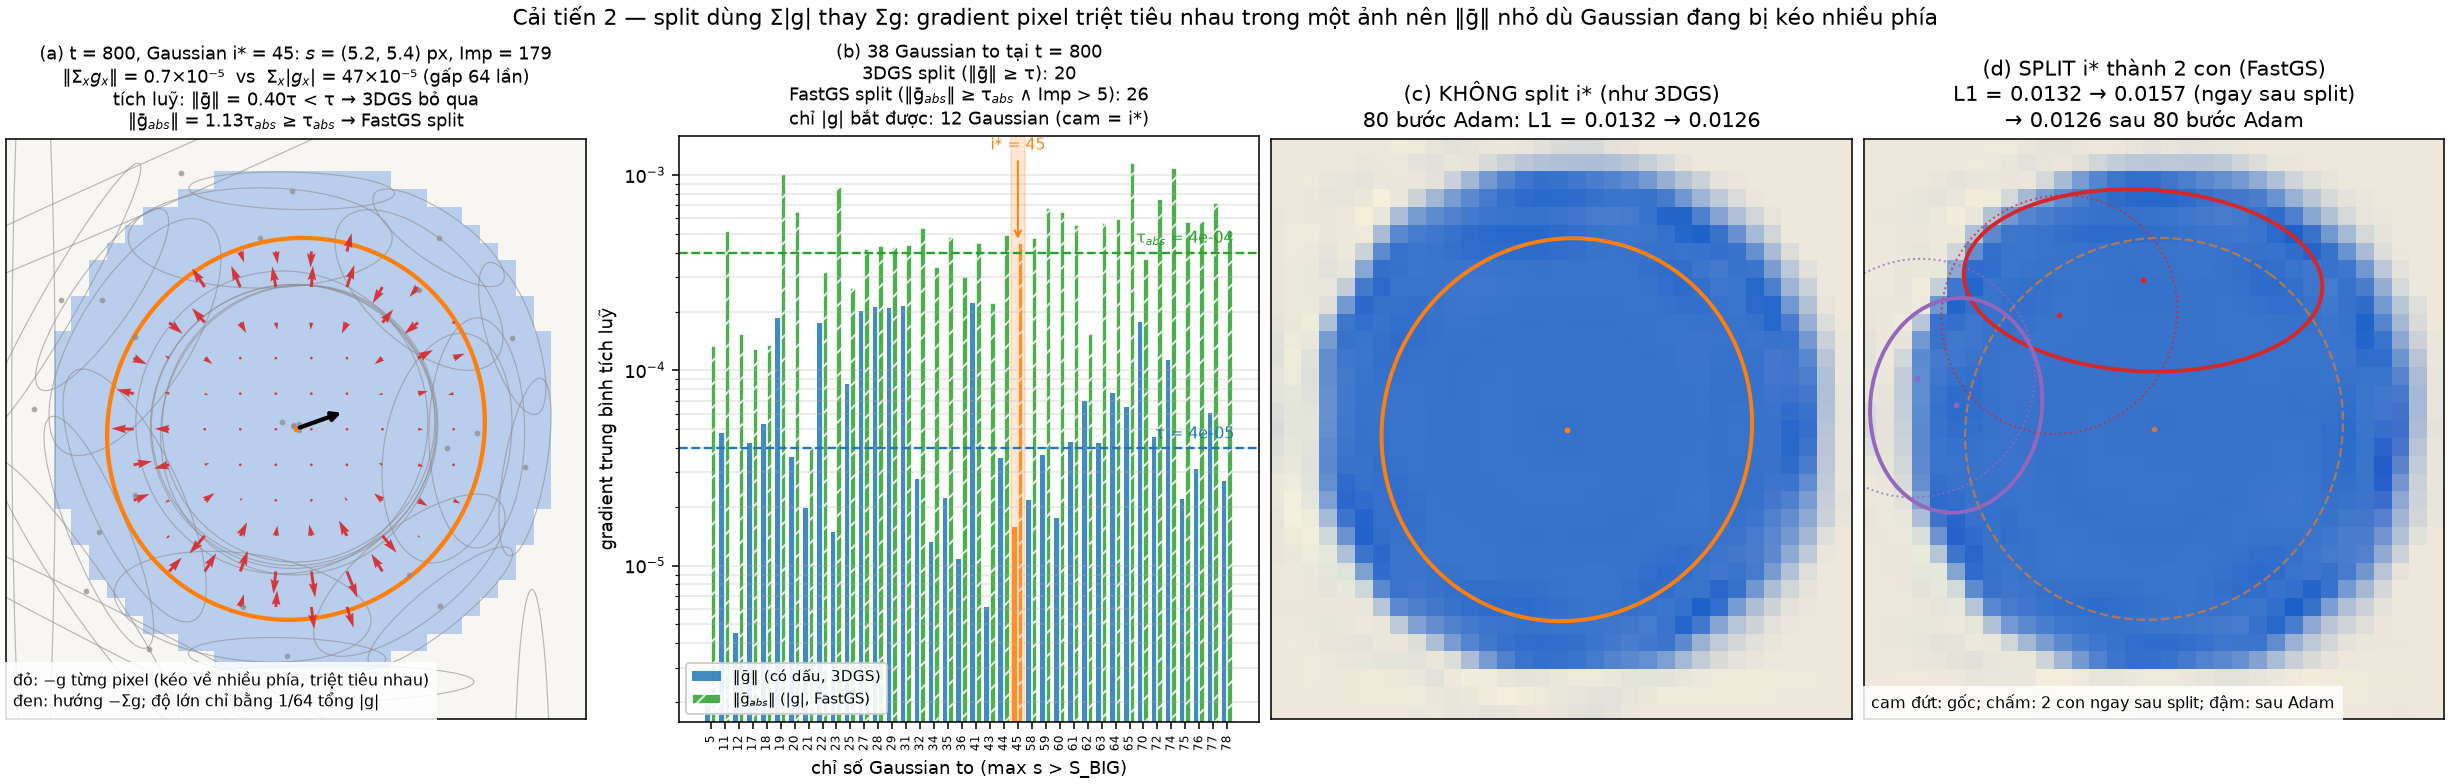
\includegraphics[width=0.72\linewidth]{7_7_abs-vs-signed-split.png}
\captionof{figure}{\footnotesize Cải tiến 2 — split dùng $\sum|g|$ thay $\sum g$: gradient pixel triệt tiêu nhau trong một ảnh nên $\|\bar g\|$ nhỏ dù Gaussian đang bị kéo nhiều phía.}
\end{frame}

% --- 7_8_prune-hard-vs-multinomial.png ---
\begin{frame}{Cải tiến 3: prune cứng vs multinomial, áp dụng trên toy}
\begin{columns}[T]
\begin{column}{0.52\textwidth}
\scriptsize
\begin{itemize}
  \item Tập ứng viên chung: $C{=}\{\alpha{<}\varepsilon_{\text{opa}} \vee \max s{>}S_{\text{HUGE}}\}$.
  \item \textbf{3DGS gốc}: xoá \textbf{ngay lập tức} toàn bộ $C$.
  \item \textbf{FastGS}: $w_i{=}1/(1{-}\text{Pruning}_i)$, rút $S{\sim}\text{Multinomial}(w,\lfloor 0.5|C|\rfloor)$, chỉ xoá $C{\cap}S$ — giữ lại ứng viên "ít đáng xoá hơn".
  \item Sau prune, FastGS áp trần $\alpha{\leftarrow}\min(\alpha,0.8)$; $\max|\Delta I|$ rất nhỏ.
\end{itemize}
\end{column}
\begin{column}{0.48\textwidth}
\centering
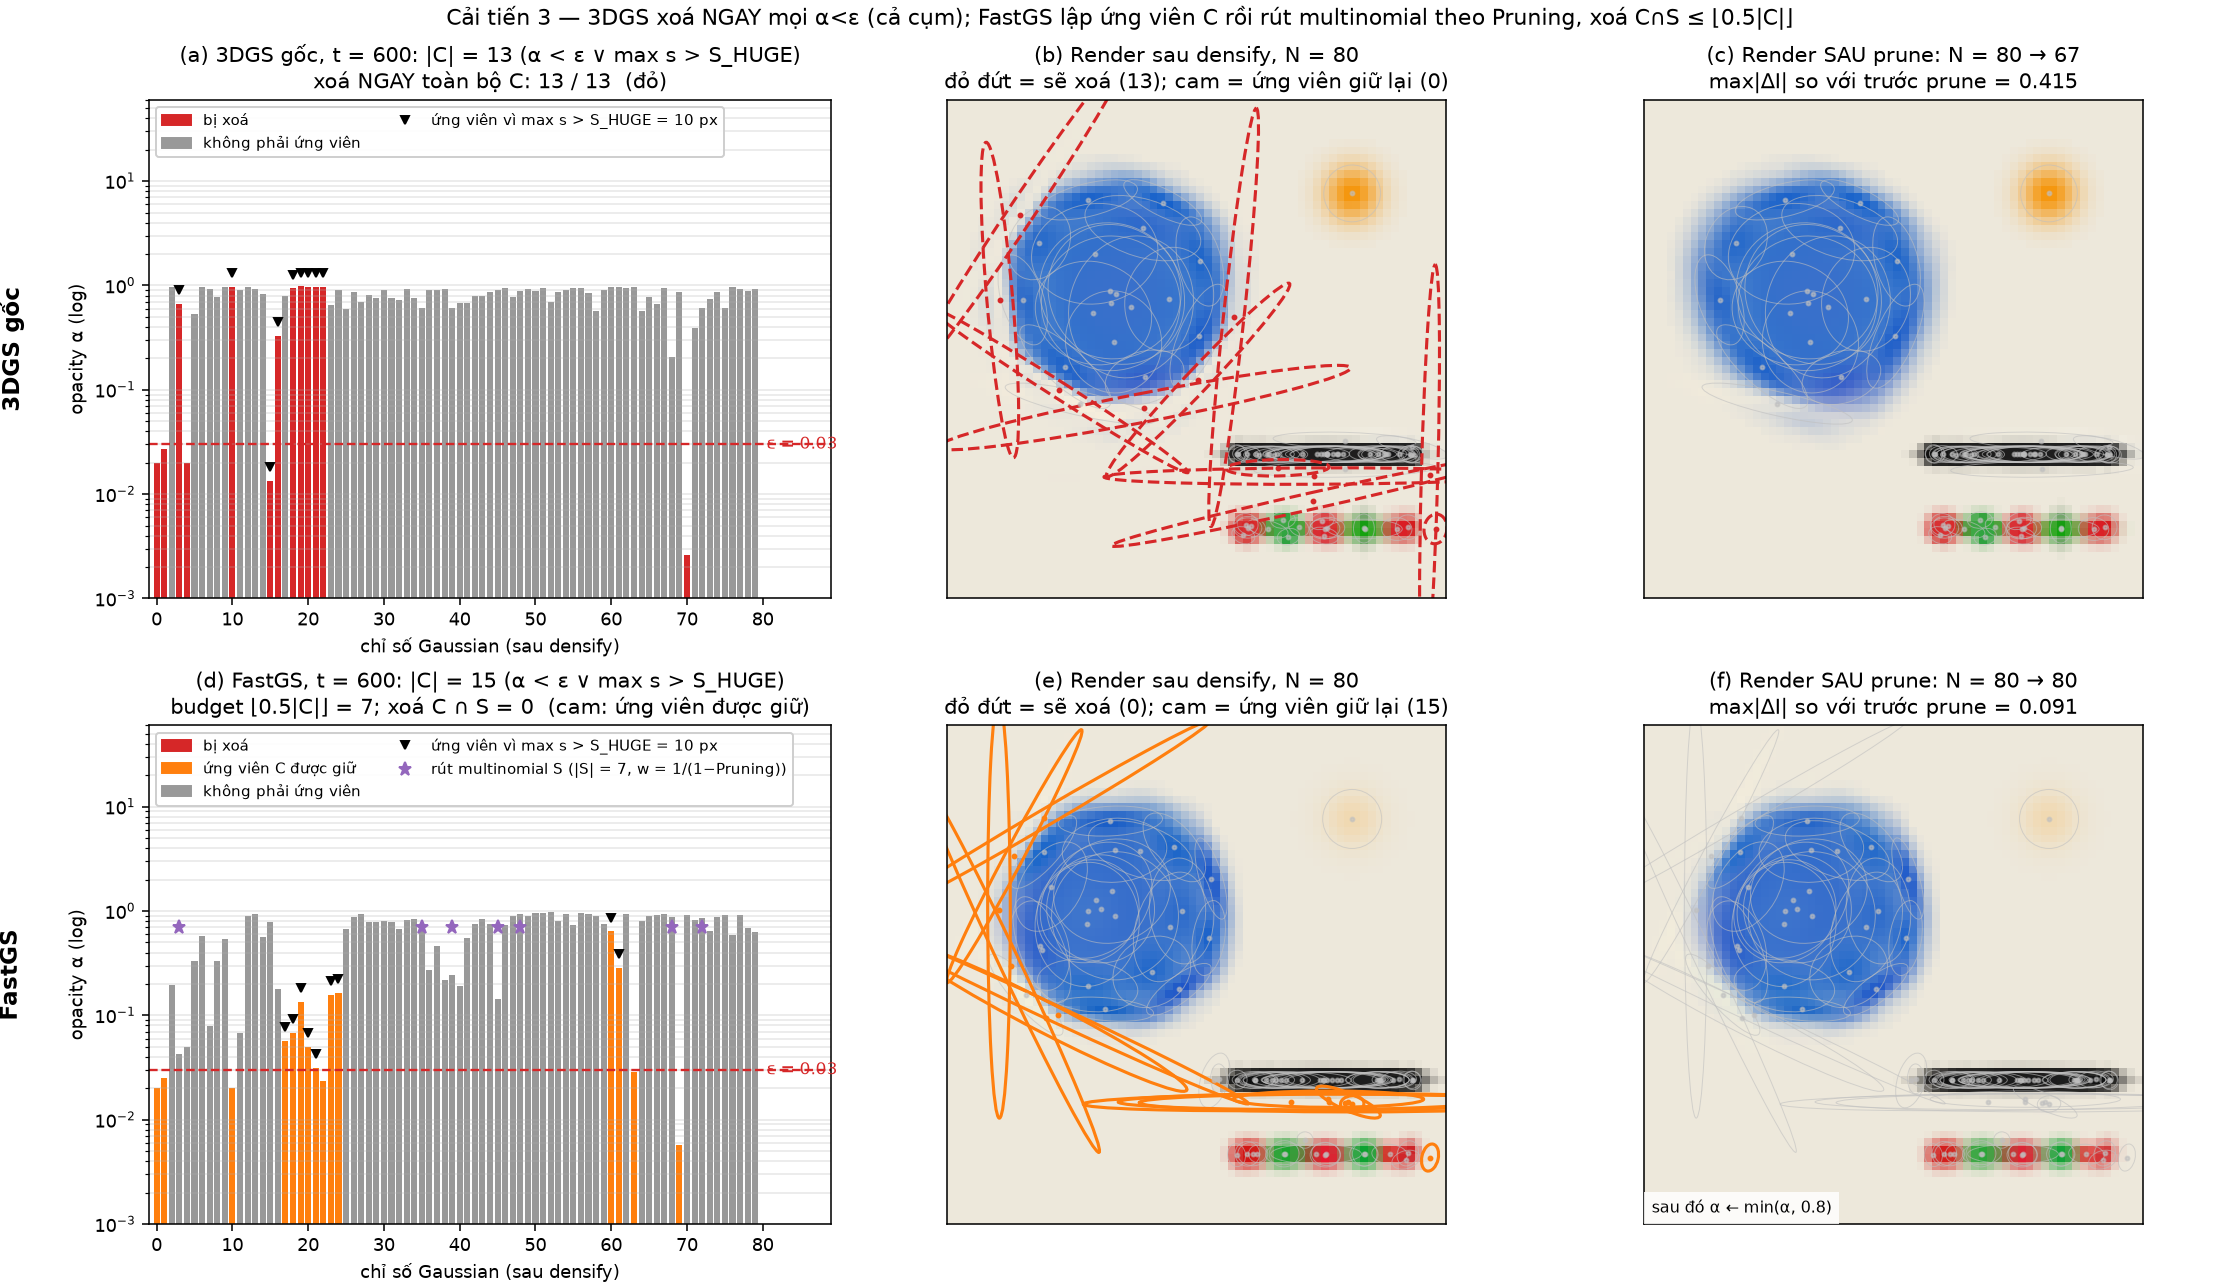
\includegraphics[width=0.95\linewidth]{7_8_prune-hard-vs-multinomial.png}
\captionof{figure}{\footnotesize 3DGS xoá NGAY mọi $\alpha{<}\varepsilon$; FastGS rút multinomial theo Pruning.}
\end{column}
\end{columns}
\end{frame}

% --- 7_9_tran-opacity-08.png ---
\begin{frame}{Cải tiến 4: tràn opacity $\alpha \leftarrow \min(\alpha, 0.8)$}
\begin{columns}[T]
\begin{column}{0.48\linewidth}
\footnotesize
\begin{itemize}
  \item Hiện tượng "tràn" opacity: khi Gaussian phía trước có $\alpha$ rất cao (ví dụ $\alpha \to 0.99$), transmittance còn lại cho lớp sau:
  \[
    T(x) = 1 - \alpha_{\text{front}}\, G_{\text{front}}(x)
  \]
  \item Tại tâm ($x=0$, $G=1$): $\alpha_{\text{front}}=0.99 \Rightarrow T(0)=0.01$; nhưng $\alpha_{\text{front}}=0.8 \Rightarrow T(0)=0.20$ — \textbf{gấp 20 lần} ánh sáng còn lại cho Gaussian phía sau.
  \item Vì $\partial L/\partial \theta_{\text{back}} \propto T \cdot \alpha_{\text{back}} \cdot G_{\text{back}}$, trần $\alpha \le 0.8$ giữ 20\% tín hiệu gradient cho lớp sau thay vì "chôn" nó vĩnh viễn.
  \item Histogram opacity cuối: đếm số Gaussian có $\alpha > 0.8$ và $\alpha > 0.99$ cho cả 3DGS gốc và FastGS-lite; bản đồ $T_{\text{end}}(x)$ trên vùng vật thể cho thấy phần trăm pixel bị "chặn hết" ($T_{\text{end}} < 0.01$) ở mỗi phương pháp.
\end{itemize}
\end{column}
\begin{column}{0.52\linewidth}
\centering
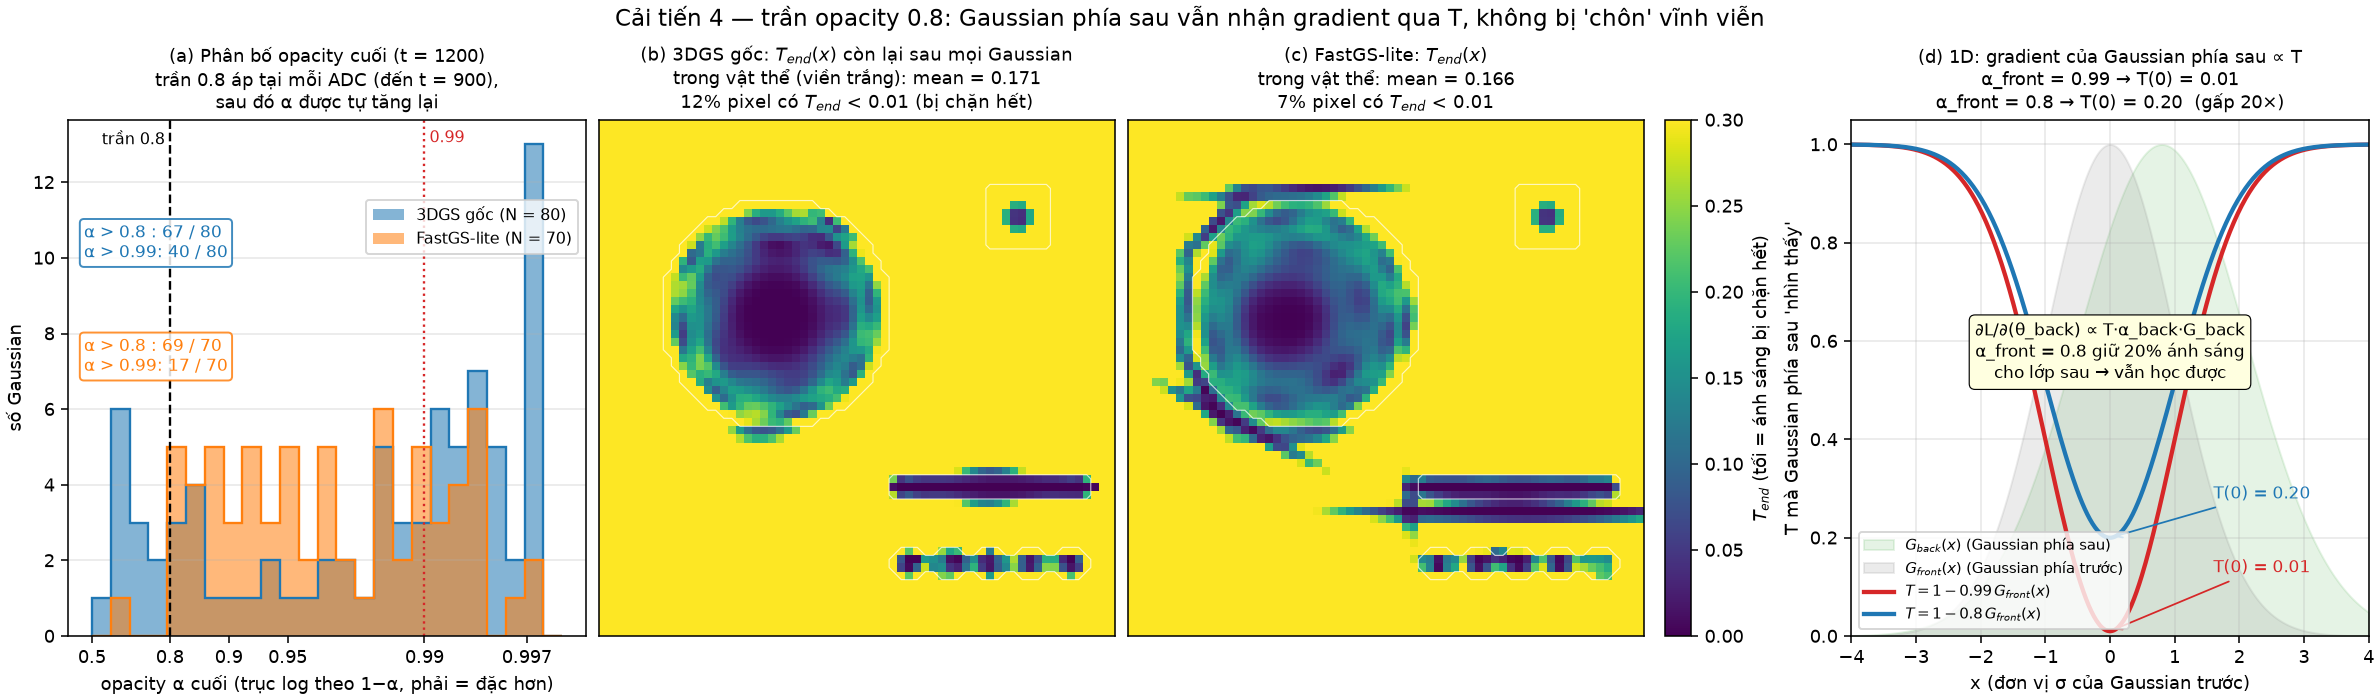
\includegraphics[width=\linewidth]{7_9_tran-opacity-08.png}
\captionof{figure}{\footnotesize Cải tiến 4 — trần opacity 0.8: Gaussian phía sau vẫn nhận gradient qua $T$, không bị "chôn" vĩnh viễn.}
\end{column}
\end{columns}
\end{frame}

% --- 7_10_final-prune-tren-toy.png ---
\begin{frame}{Cải tiến 5: final prune trên toy — khép lại chương ADC}
\begin{columns}[T]
\begin{column}{0.52\textwidth}
\scriptsize
\begin{itemize}
  \item Sau densify (kết thúc $t{=}900$), FastGS-lite chạy \textbf{final prune} tại $t{\in}(1000,1100)$: $\text{rm}{=}[\alpha{<}0.1] \vee [\text{Pruning}{>}0.9]$.
  \item \textbf{3DGS gốc không có bước này} — $N(t)$ phẳng $[900,1200]$; FastGS giảm "hai bậc thang" tại $1000,1100$.
  \item Scatter $(\alpha,\text{Pruning})$: vùng "chữ L" bị xoá ($\alpha$ thấp, Pruning cao), đánh dấu X đỏ.
  \item $L_1$ cuối FastGS-lite tương đương 3DGS nhưng $N$ nhỏ hơn — kết quả gọn nhất, khép lại chương ADC.
\end{itemize}
\end{column}
\begin{column}{0.48\textwidth}
\centering
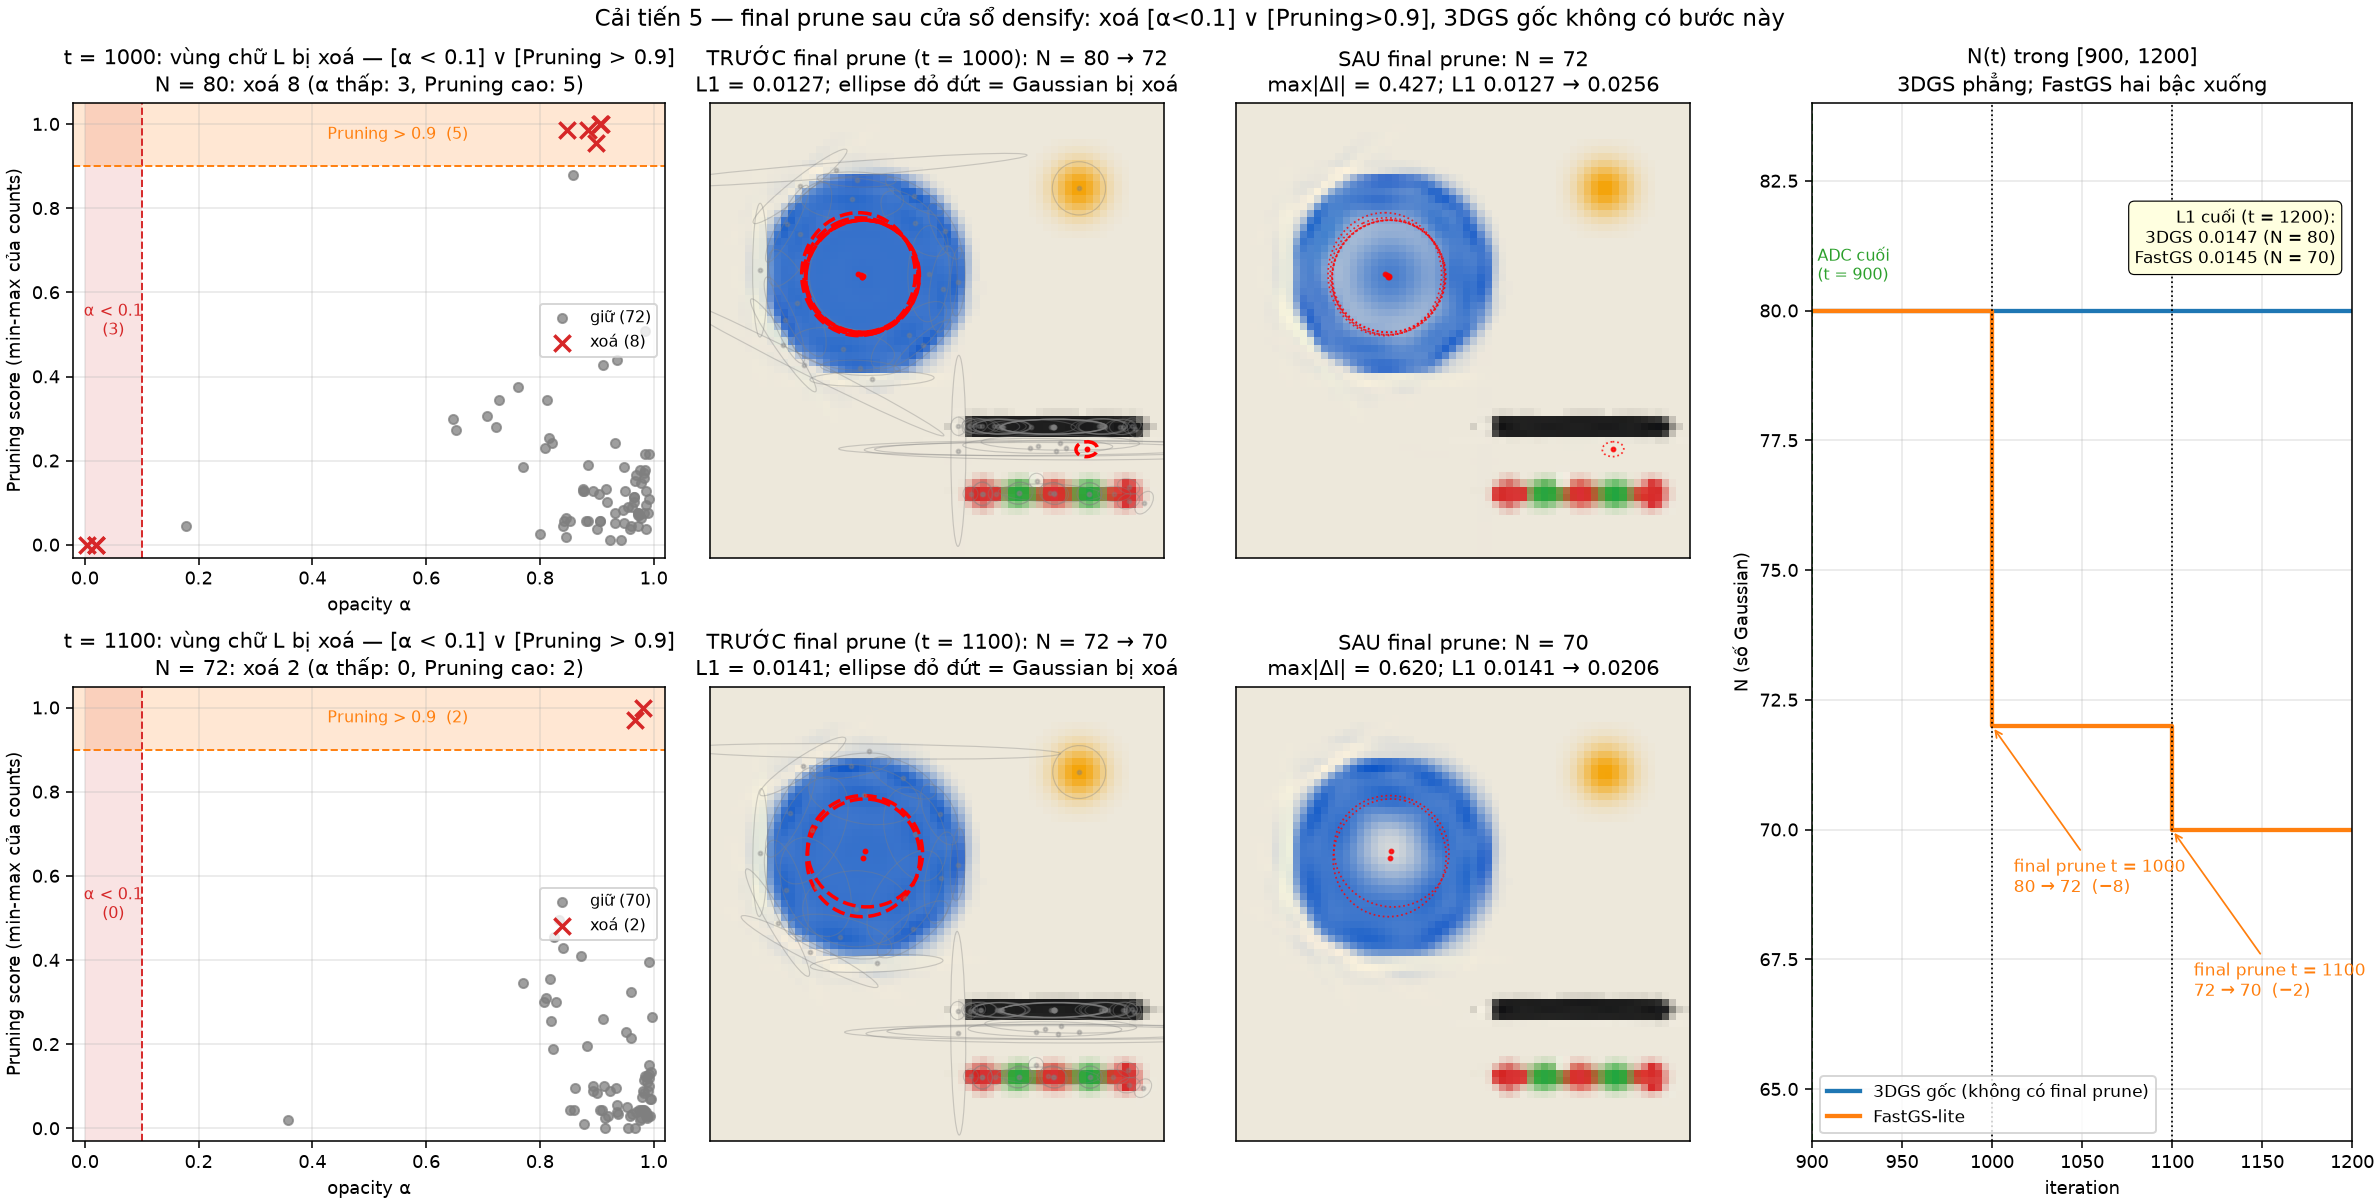
\includegraphics[width=0.95\linewidth]{7_10_final-prune-tren-toy.png}
\captionof{figure}{\footnotesize Final prune sau densify: xoá $[\alpha{<}0.1]\vee[\text{Pruning}{>}0.9]$.}
\end{column}
\end{columns}
\end{frame}


\section{ADC chuyên sâu — Cơ chế theo dòng thời gian}
% ============================================================
% Phan ADC-TLa: Adaptive Density Control - nhom minh hoa "co che theo
% dong thoi gian" tu notebook adc\_3dgs (doc lap voi nhom adc\_figures)
% 9 frame, dung dung 9 anh fig\_01..fig\_09 trong adc\_3dgs/figures
% ============================================================

% --- fig_01_timeline.png ---
\begin{frame}{ADC nhìn theo dòng thời gian: lịch chạy đầy đủ}
\scriptsize
\begin{itemize}
    \item Vòng đời huấn luyện: $T{=}30000$ vòng, 4 giai đoạn chồng lấp.
    \item \textbf{(a) Tích luỹ gradient}: mọi vòng $t{<}15000$.
    \item \textbf{(b) Densify+prune}: khi $t{>}500$ và $t\bmod 100{=}0$ $\Rightarrow$ 144 mốc ($t{=}600,700,\dots,14900$).
    \item \textbf{(c) Reset opacity}: $t\bmod 3000{=}0$, $t{<}15000$ $\Rightarrow$ 4 mốc $\{3000,6000,9000,12000\}$.
    \item \textbf{(d) N đóng băng}: $t{\geq}15000$, chỉ tối ưu $\theta{=}(\mu,s,q,\alpha,\text{SH})$.
\end{itemize}
\centering
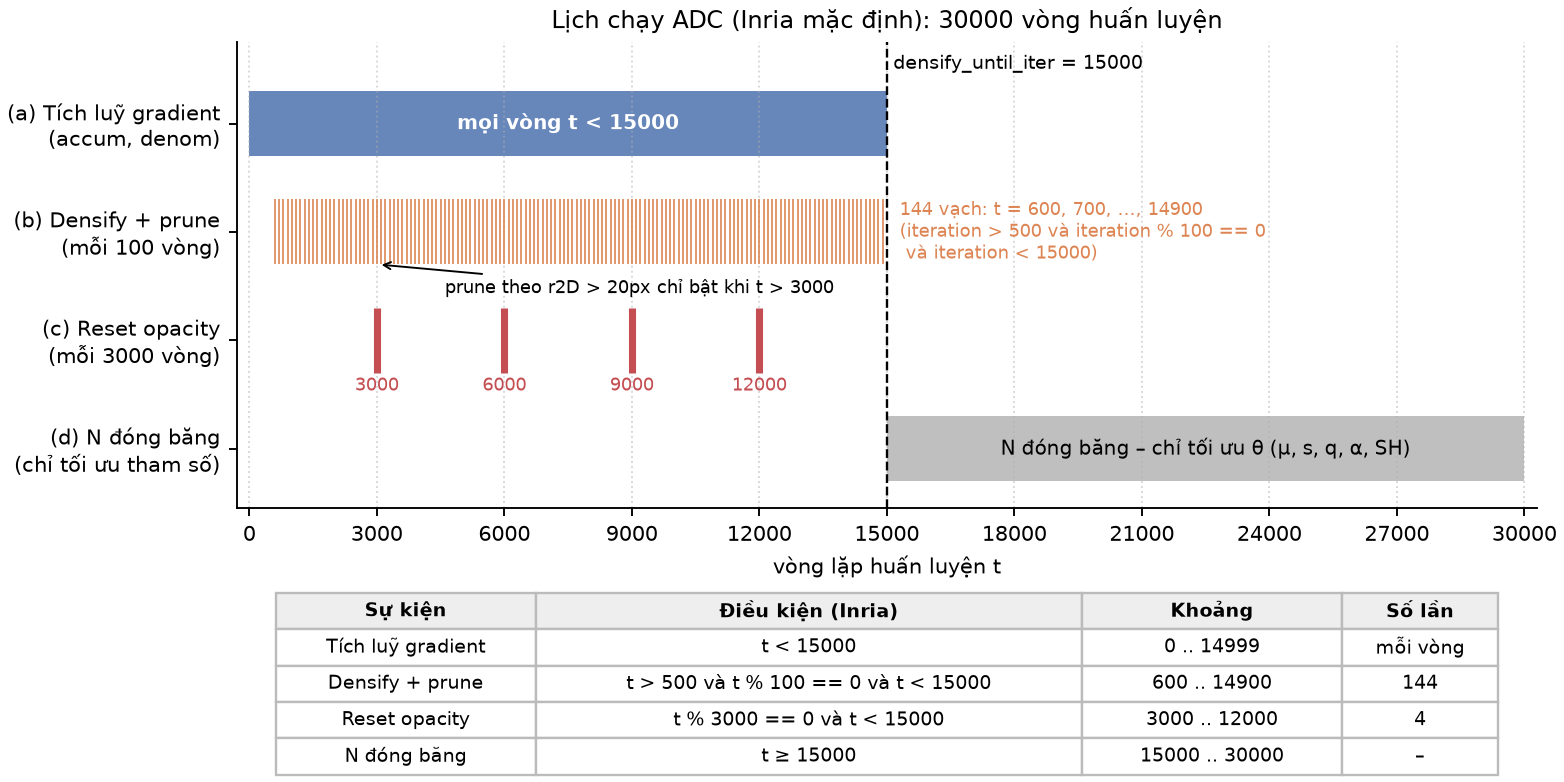
\includegraphics[width=0.6\linewidth]{fig_01_timeline.png}
\captionof{figure}{\footnotesize Lịch chạy ADC 30000 vòng.}
\end{frame}

% --- fig_02_accum_denom.png ---
\begin{frame}{Tích luỹ gradient: accum, denom và $\bar g$}
\begin{columns}
\begin{column}{0.5\linewidth}
\footnotesize
\begin{itemize}
    \item Mỗi Gaussian $i$ giữ 2 bộ đếm cộng dồn giữa 2 lần densify (chu kỳ 100 vòng):
    \[
    \mathrm{accum}_i(t) = \sum_{t' \le t} \mathbb{1}_i(t')\,\Big\|\sum_x \tfrac{\partial L}{\partial \mu'_i}\Big\|
    \]
    \[
    \mathrm{denom}_i(t) = \sum_{t' \le t} \mathbb{1}_i(t')
    \]
    \item $\mathbb{1}_i(t)$: Gaussian $i$ có được chiếu vào khung hình tại vòng $t$ hay không (bị che $\Rightarrow$ không cộng).
    \item Gradient trung bình: $\bar g_i = \mathrm{accum}_i/\mathrm{denom}_i$.
    \item Ví dụ mô phỏng 100 vòng: bị che liên tục 12 vòng ($t{=}40..52$) $\Rightarrow$ cả accum và denom đi ngang.
    \item Tại $t=100$: $\bar g_i \approx 3$–$4\times 10^{-4} \ge \tau_{grad}=2\times10^{-4}$ $\Rightarrow$ ứng viên densify.
\end{itemize}
\end{column}
\begin{column}{0.5\linewidth}
\centering
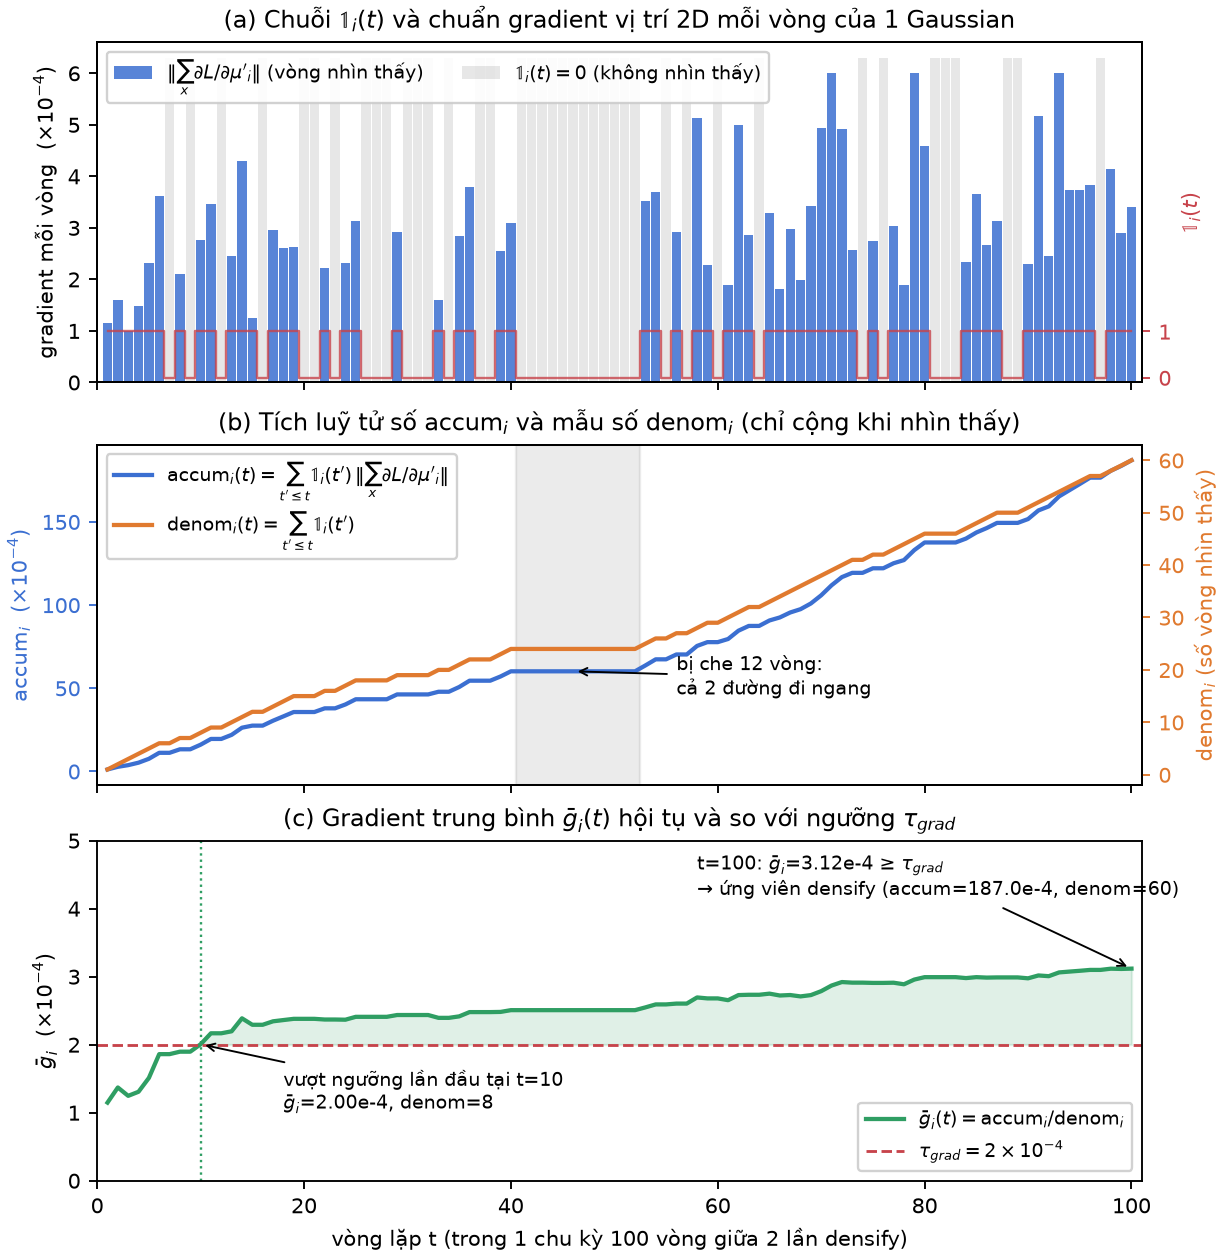
\includegraphics[width=\linewidth]{fig_02_accum_denom.png}
\captionof{figure}{\footnotesize (a) chuỗi $\mathbb{1}_i(t)$ và gradient mỗi vòng; (b) accum/denom cộng dồn; (c) $\bar g_i(t)$ so với $\tau_{grad}$.}
\end{column}
\end{columns}
\end{frame}

% --- fig_03_grad_cancel.png ---
\begin{frame}{Hiện tượng triệt tiêu gradient (gradient cancellation)}
\footnotesize
\begin{itemize}
    \item Inria chỉ tích luỹ \textbf{chuẩn của tổng có dấu} $\big\|\sum_x \partial L/\partial \mu'_i\big\|$, KHÔNG dùng tổng các chuẩn $\sum_x \|\partial L/\partial \mu'_i|_x\|$.
    \item Với $L=\tfrac12\sum_x (I(x)-I_{gt}(x))^2$ và $I(x)=\alpha e^{-\|x-\mu\|^2/2\sigma^2}$: $\dfrac{\partial L}{\partial \mu} = \sum_x \big(I(x)-I_{gt}(x)\big)\dfrac{I(x)}{\sigma^2}(x-\mu)$.
    \item Trường hợp (a) \emph{lệch vị trí}: các vector $g_x$ cùng thiên hướng $\Rightarrow$ tổng có dấu lớn, gần bằng tổng chuẩn.
    \item Trường hợp (b) \emph{đúng vị trí nhưng sai kích thước} (Gaussian to hơn GT, đồng tâm): các $g_x$ đối xứng quanh tâm, triệt tiêu lẫn nhau $\Rightarrow$ $\|\sum_x g_x\|$ rất nhỏ so với $\sum_x\|g_x\|$ (tỉ số chỉ cỡ $10^{-1}$–$10^{-2}$ trong ví dụ minh hoạ).
    \item Hệ quả: $\bar g_i$ nhỏ $\Rightarrow$ \textbf{không được densify} dù ảnh dựng vẫn sai — điểm mù đã biết của tiêu chí gradient cổ điển 3DGS.
\end{itemize}
\begin{center}
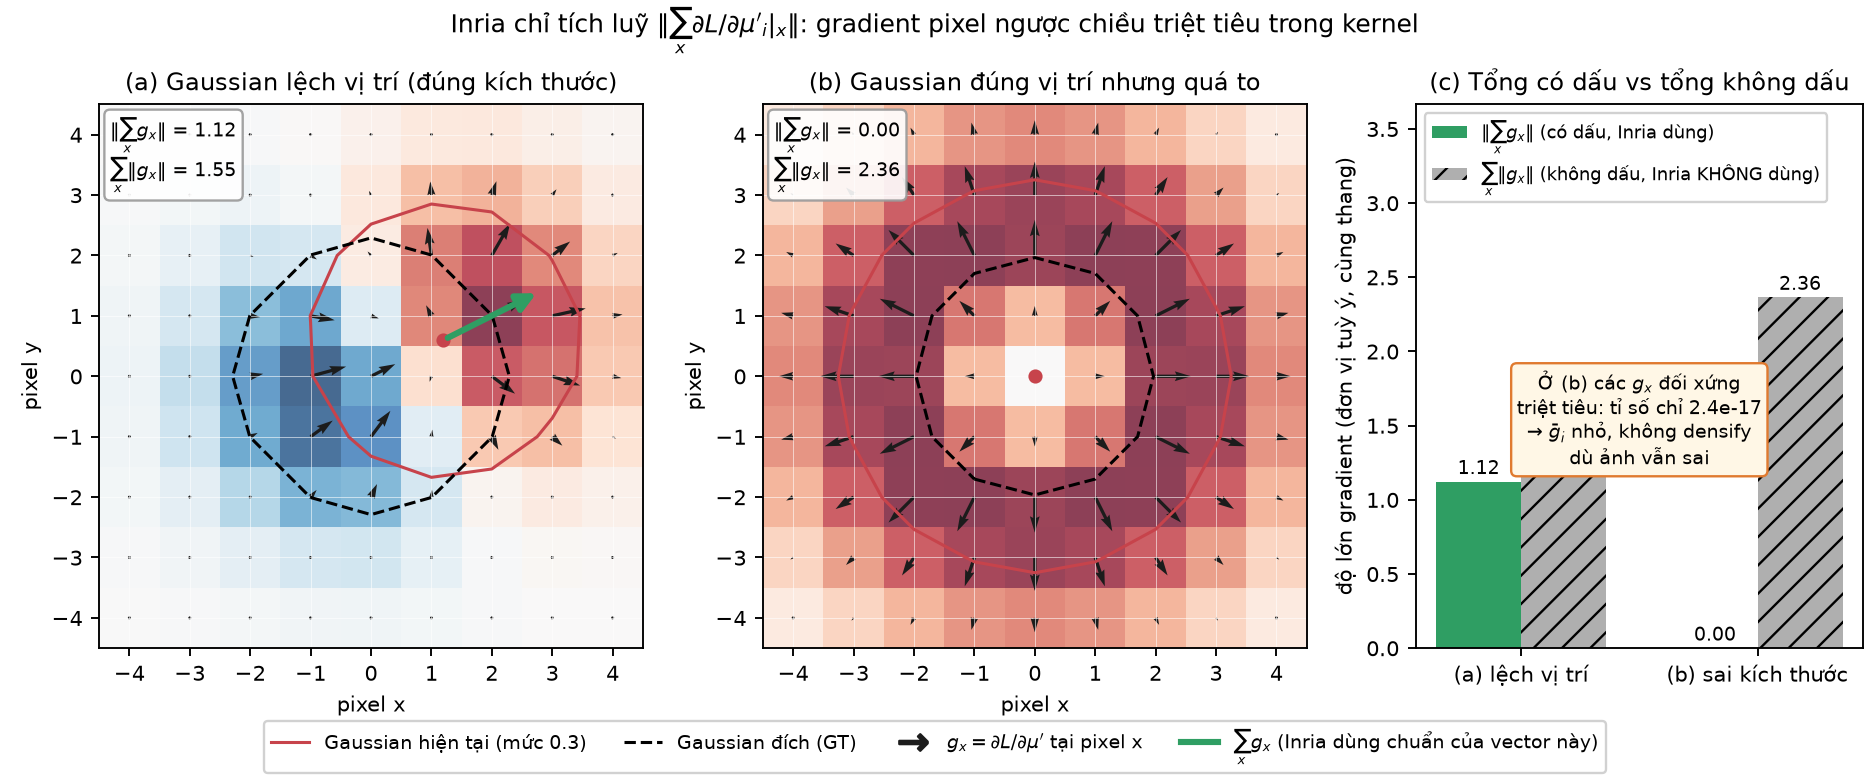
\includegraphics[width=0.72\linewidth]{fig_03_grad_cancel.png}
\captionof{figure}{\footnotesize (a) lệch vị trí: gradient cộng dồn mạnh; (b) sai kích thước, đối xứng: gradient triệt tiêu; (c) so sánh tổng có dấu vs không dấu.}
\end{center}
\end{frame}

% --- fig_04_gbar_history.png ---
\begin{frame}{Lịch sử $\bar g_i(t)$ của một Gaussian qua nhiều vòng}
\begin{columns}[T]
\begin{column}{0.52\textwidth}
\scriptsize
\begin{itemize}
    \item Mô phỏng $T{=}15000$ vòng, 5 loại Gaussian: viền vật thể, gần viền, nền phẳng, thỉnh thoảng bị che, mới sinh (clone tại $t{=}3000$).
    \item $\mathrm{accum}_i,\mathrm{denom}_i$ bị xoá về 0 mỗi mốc densify ($t\bmod 100{=}0$) $\Rightarrow$ $\bar g_i(t)$ dạng răng cưa.
    \item Viền vật thể: $\bar g_i \sim \exp(-t/5500)$, có xung tăng sau reset opacity ($t{=}3000,6000,9000,12000$).
    \item ``Bị che'' ($p_{vis}{=}0.3$): denom nhỏ $\Rightarrow$ dao động mạnh, có thể vượt $\tau_{grad}{=}2{\times}10^{-4}$ giả tạo.
\end{itemize}
\end{column}
\begin{column}{0.48\textwidth}
\centering
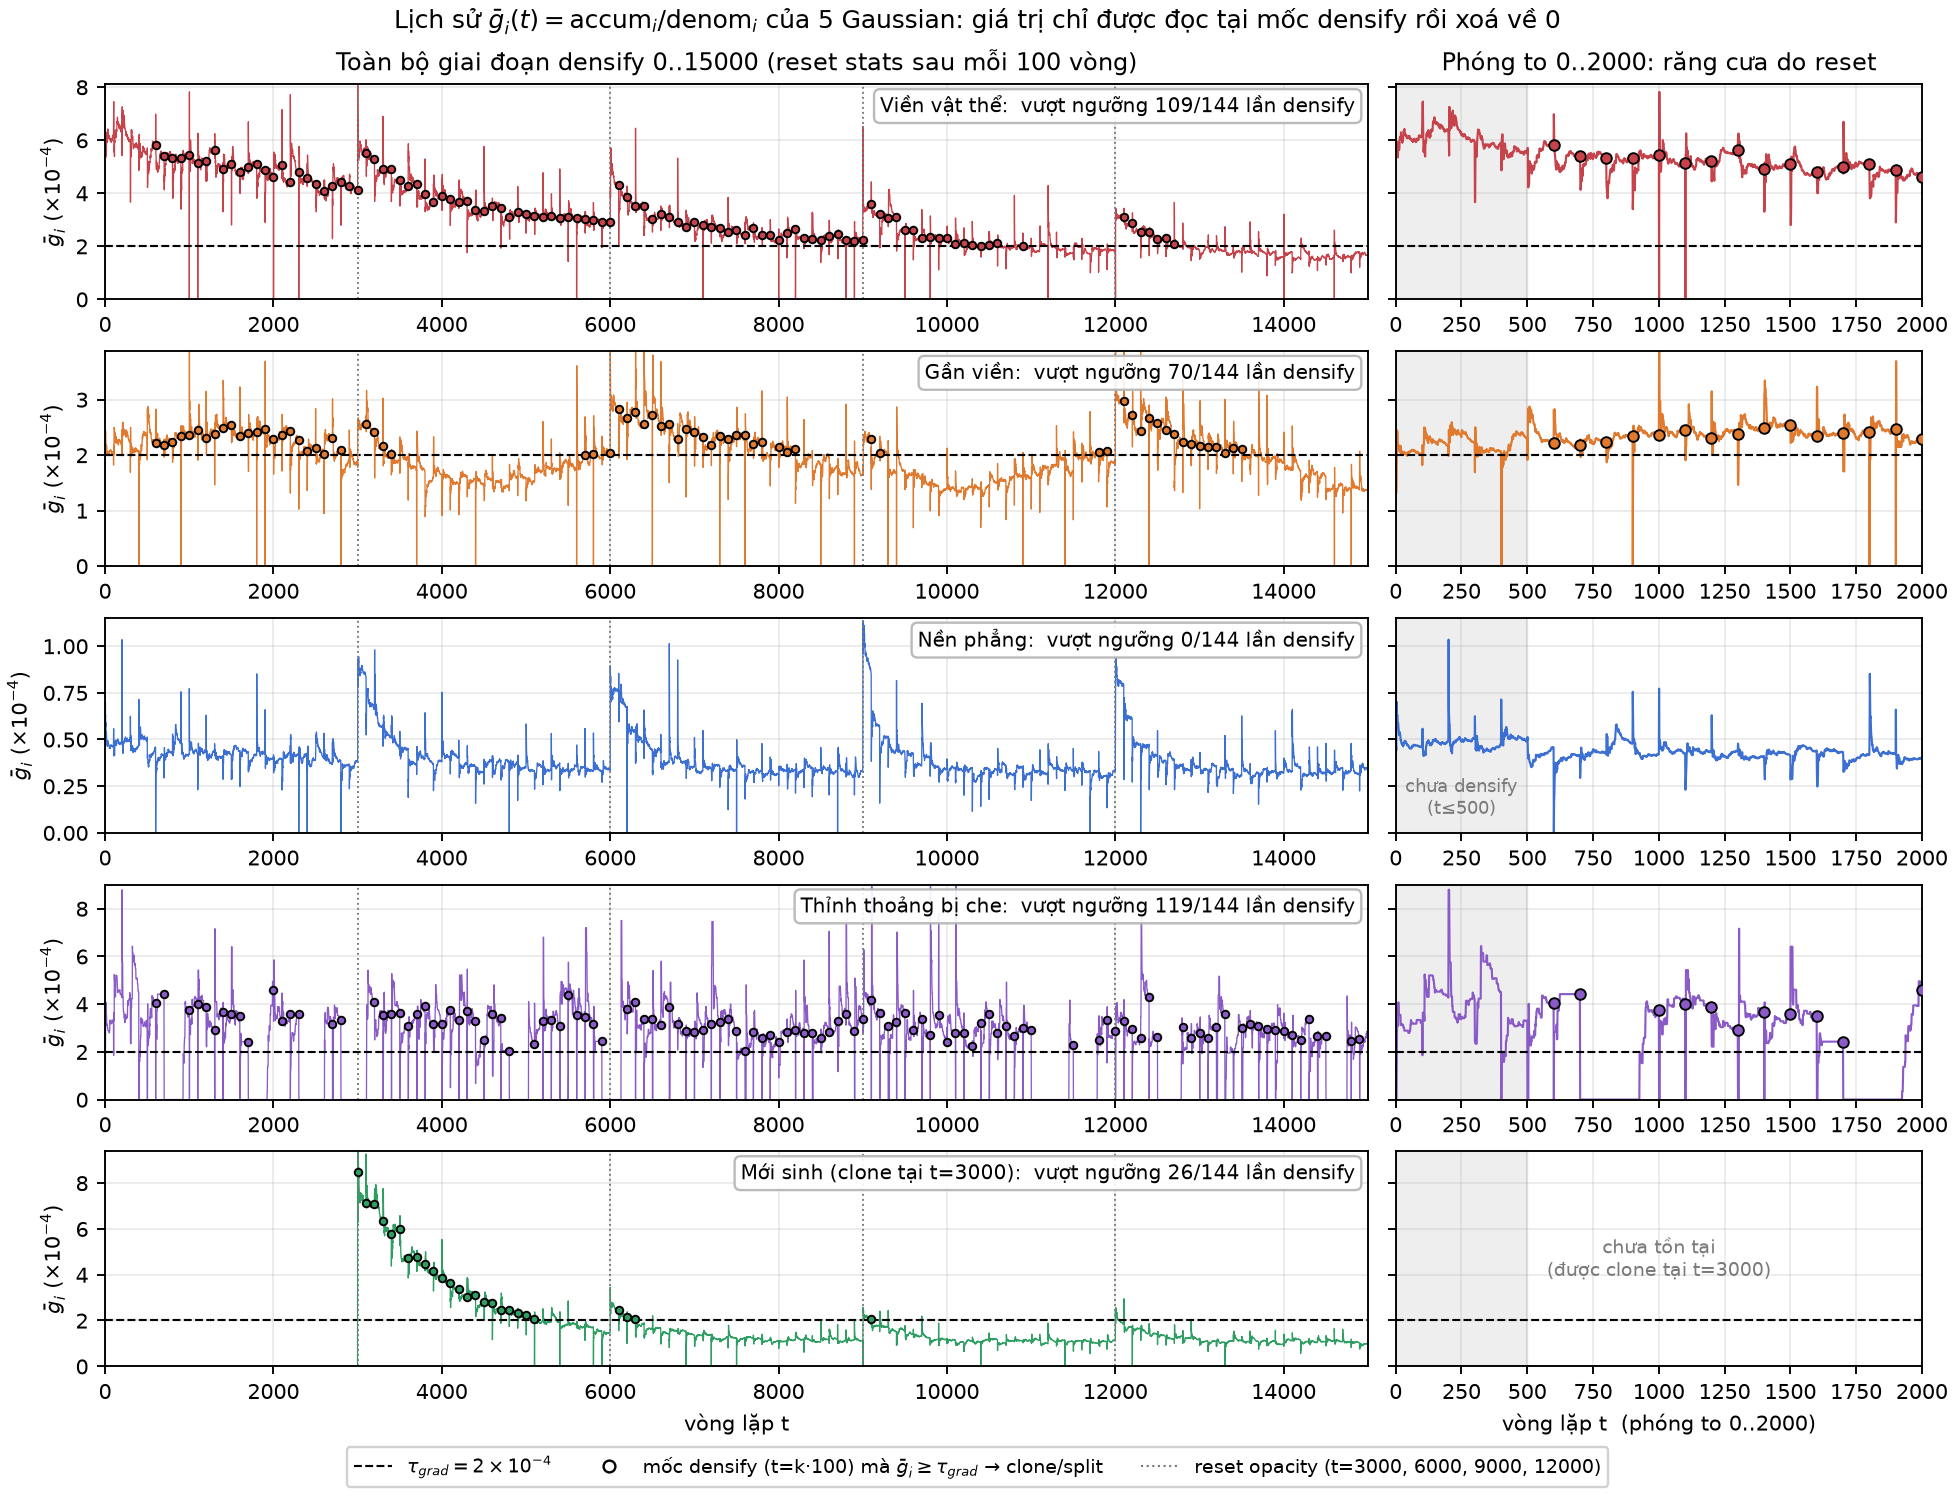
\includegraphics[width=0.95\linewidth]{fig_04_gbar_history.png}
\captionof{figure}{\footnotesize $\bar g_i(t)$ của 5 Gaussian, răng cưa do reset thống kê mỗi 100 vòng.}
\end{column}
\end{columns}
\end{frame}

% --- fig_05_decision_plane.png ---
\begin{frame}{Mặt phẳng quyết định: giữ nguyên / clone / split}
\begin{columns}
\begin{column}{0.55\linewidth}
\footnotesize
\begin{itemize}
    \item Công thức quyết định (dùng $\tau_{grad}=2\times10^{-4}$, $\delta=\texttt{percent\_dense}=0.01$):
    \[
    \text{clone}_i = [\|\bar g_i\| \ge \tau_{grad}] \wedge [\max(s_i) \le \delta\cdot\text{extent}]
    \]
    \[
    \text{split}_i = [\|\bar g_i\| \ge \tau_{grad}] \wedge [\max(s_i) > \delta\cdot\text{extent}]
    \]
    \item Trục ngang: $\|\bar g_i\|$ (log); trục dọc: $\max(s_i)/\text{extent}$ (log).
    \item Ngưỡng prune riêng theo kích thước: $\max(s_i) > 0.1\cdot\text{extent}$ (gạch chéo phía trên).
    \item Điểm ví dụ: E nằm đúng biên $\ge,\le$ $\Rightarrow$ clone; F vượt cả $\tau_{grad}$ lẫn ngưỡng prune $\Rightarrow$ split rồi bị prune ngay bước sau.
\end{itemize}
\end{column}
\begin{column}{0.45\linewidth}
\centering
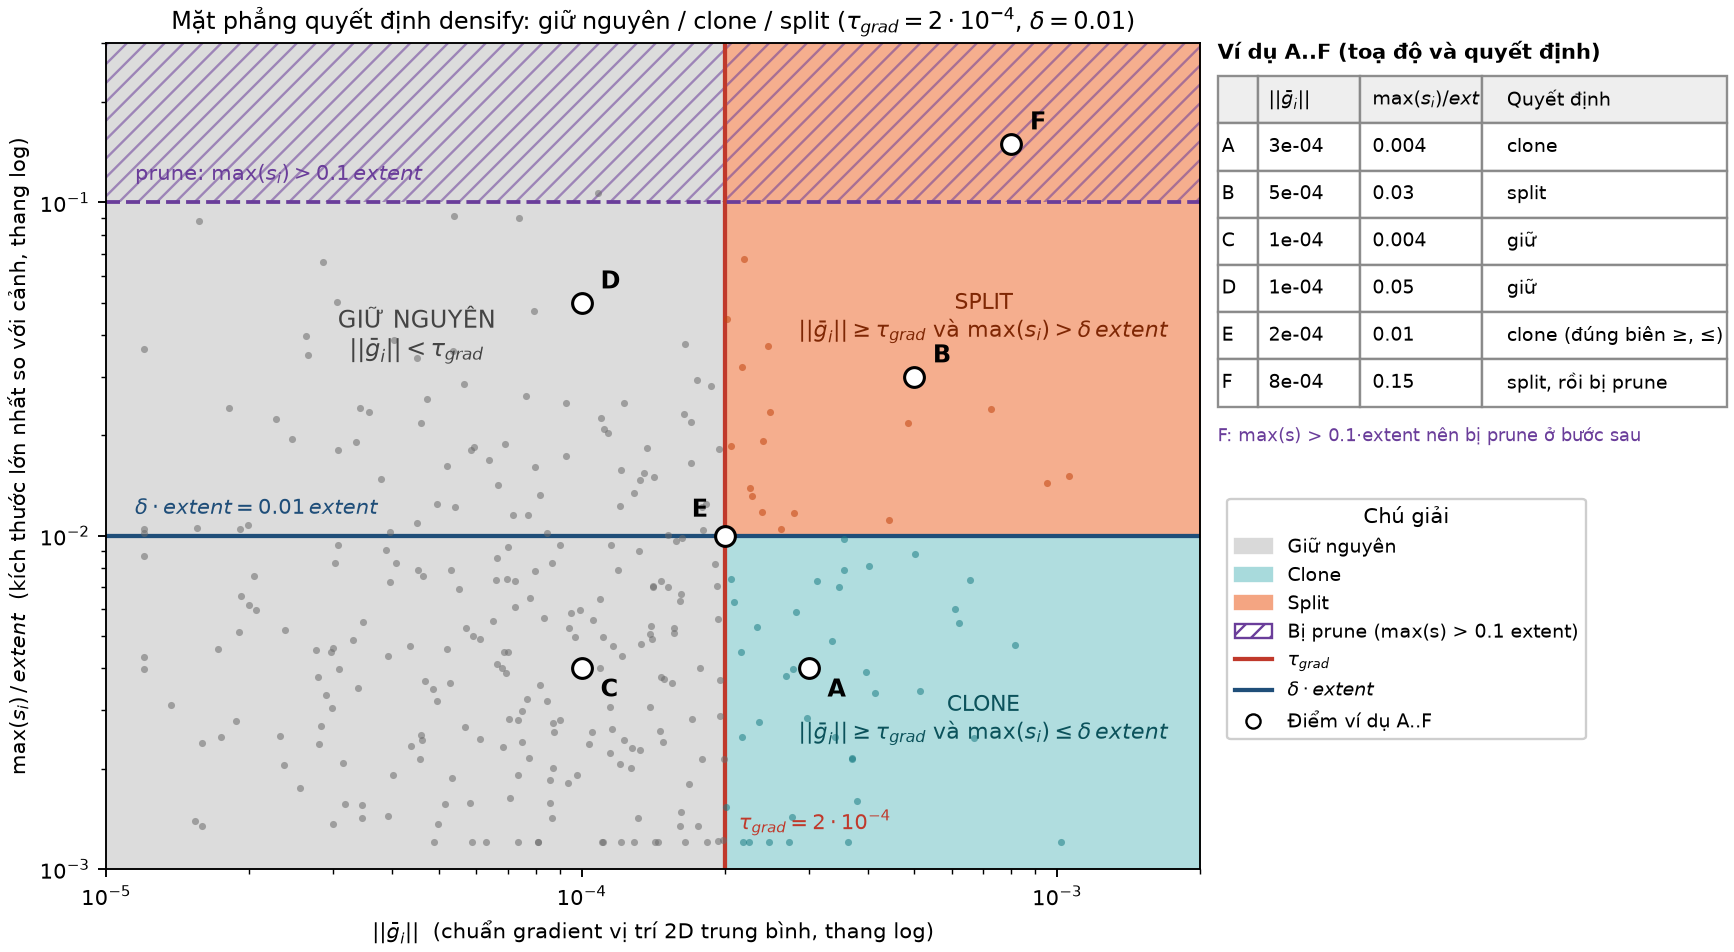
\includegraphics[width=\linewidth]{fig_05_decision_plane.png}
\captionof{figure}{\footnotesize 3 vùng: giữ nguyên / clone / split, cùng 6 điểm ví dụ A--F và vùng bị prune theo kích thước.}
\end{column}
\end{columns}
\end{frame}

% --- fig_06_scene_extent.png ---
\begin{frame}{Đo phạm vi cảnh (scene extent) và chuẩn hoá ngưỡng}
\footnotesize
\begin{itemize}
    \item Inria tính \texttt{cameras\_extent} = $1.1 \times d_{max}$, với $d_{max}$ là khoảng cách xa nhất từ một camera tới \emph{tâm} của tập camera: $\text{extent} = 1.1 \max_k \|c_k - \bar c\|$.
    \item Đây là chuẩn hoá theo \emph{không gian}, không phải theo pixel — cùng một $\delta=0.01$ nhưng ngưỡng tuyệt đối $\delta\cdot\text{extent}$ thay đổi theo kích thước thật của cảnh.
    \item Ba mức ngưỡng theo tỉ lệ cố định $1:10:100$: $0.01\cdot\text{extent}$ (ranh giới clone/split), $0.1\cdot\text{extent}$ (ranh giới prune theo kích thước), và extent (kích thước toàn cảnh).
    \item Minh hoạ: 2 Gaussian ví dụ vẽ đúng theo 2 ngưỡng $\delta\cdot\text{extent}$ và $\texttt{PRUNE\_SCALE}\cdot\text{extent}=0.1\cdot\text{extent}$ để thấy chênh lệch kích thước tuyệt đối.
\end{itemize}
\begin{center}
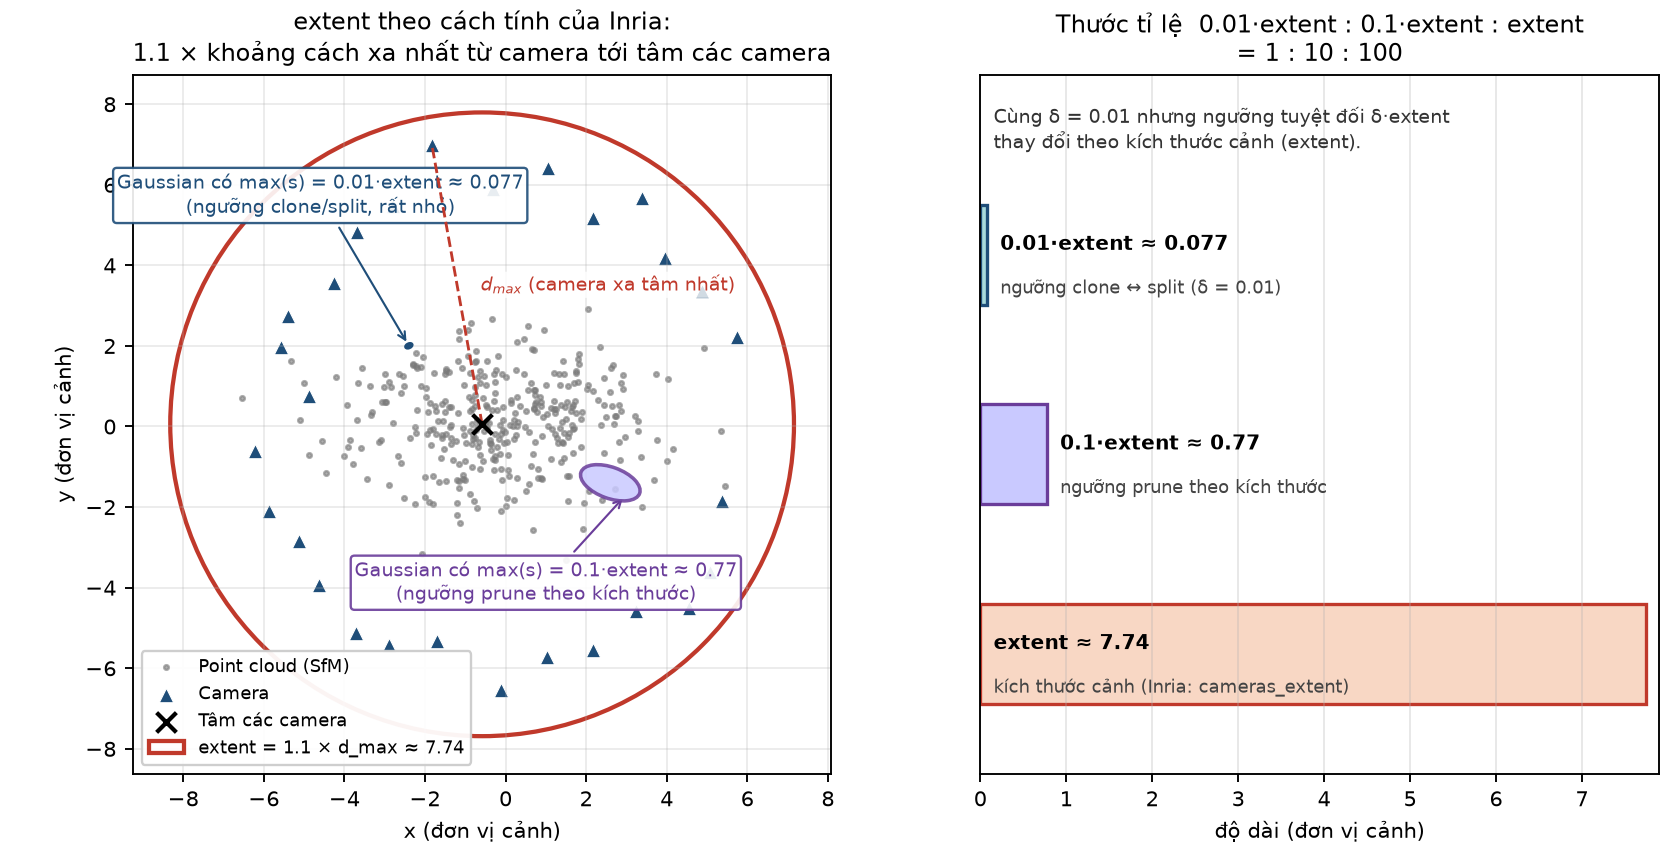
\includegraphics[width=0.68\linewidth]{fig_06_scene_extent.png}
\captionof{figure}{\footnotesize Trái: camera quanh point cloud, bán kính extent $=1.1\,d_{max}$; phải: thước tỉ lệ $0.01$–$0.1$–$1\times$ extent.}
\end{center}
\end{frame}

% --- fig_07_threshold_sweep.png ---
\begin{frame}{Quét ngưỡng: đánh đổi thêm nhiều vs thêm ít}
\footnotesize
\begin{itemize}
    \item Mô phỏng $N=10000$ Gaussian, $\|\bar g_i\|$ log-normal (trung vị $\approx 4\times10^{-5}$), $\max(s_i)/\text{extent}$ log-normal (trung vị $\approx 0.004$).
    \item Với $\tau_{grad}=2\times10^{-4}$ mặc định: chỉ một phần nhỏ Gaussian vượt ngưỡng và được đưa vào densify (phần đuôi dài của phân phối).
    \item Quét $\tau_{grad}$ trong $[5\times10^{-5}, 10^{-3}]$: ngưỡng càng nhỏ, tỉ lệ \% Gaussian được densify tăng mạnh (đường cong dốc quanh vùng mặc định) — đây là đánh đổi cốt lõi: ngưỡng thấp $\Rightarrow$ thêm nhiều Gaussian (tốn bộ nhớ/tính toán), ngưỡng cao $\Rightarrow$ bỏ sót chi tiết.
    \item Quét $\delta$ trong $[0.002, 0.05]$ (giữ $\tau_{grad}$ cố định): $\delta$ lớn hơn $\Rightarrow$ tỉ lệ clone tăng, tỉ lệ split giảm (đường \%clone và \%split cắt nhau đối xứng quanh $\delta=0.01$ mặc định).
\end{itemize}
\begin{center}
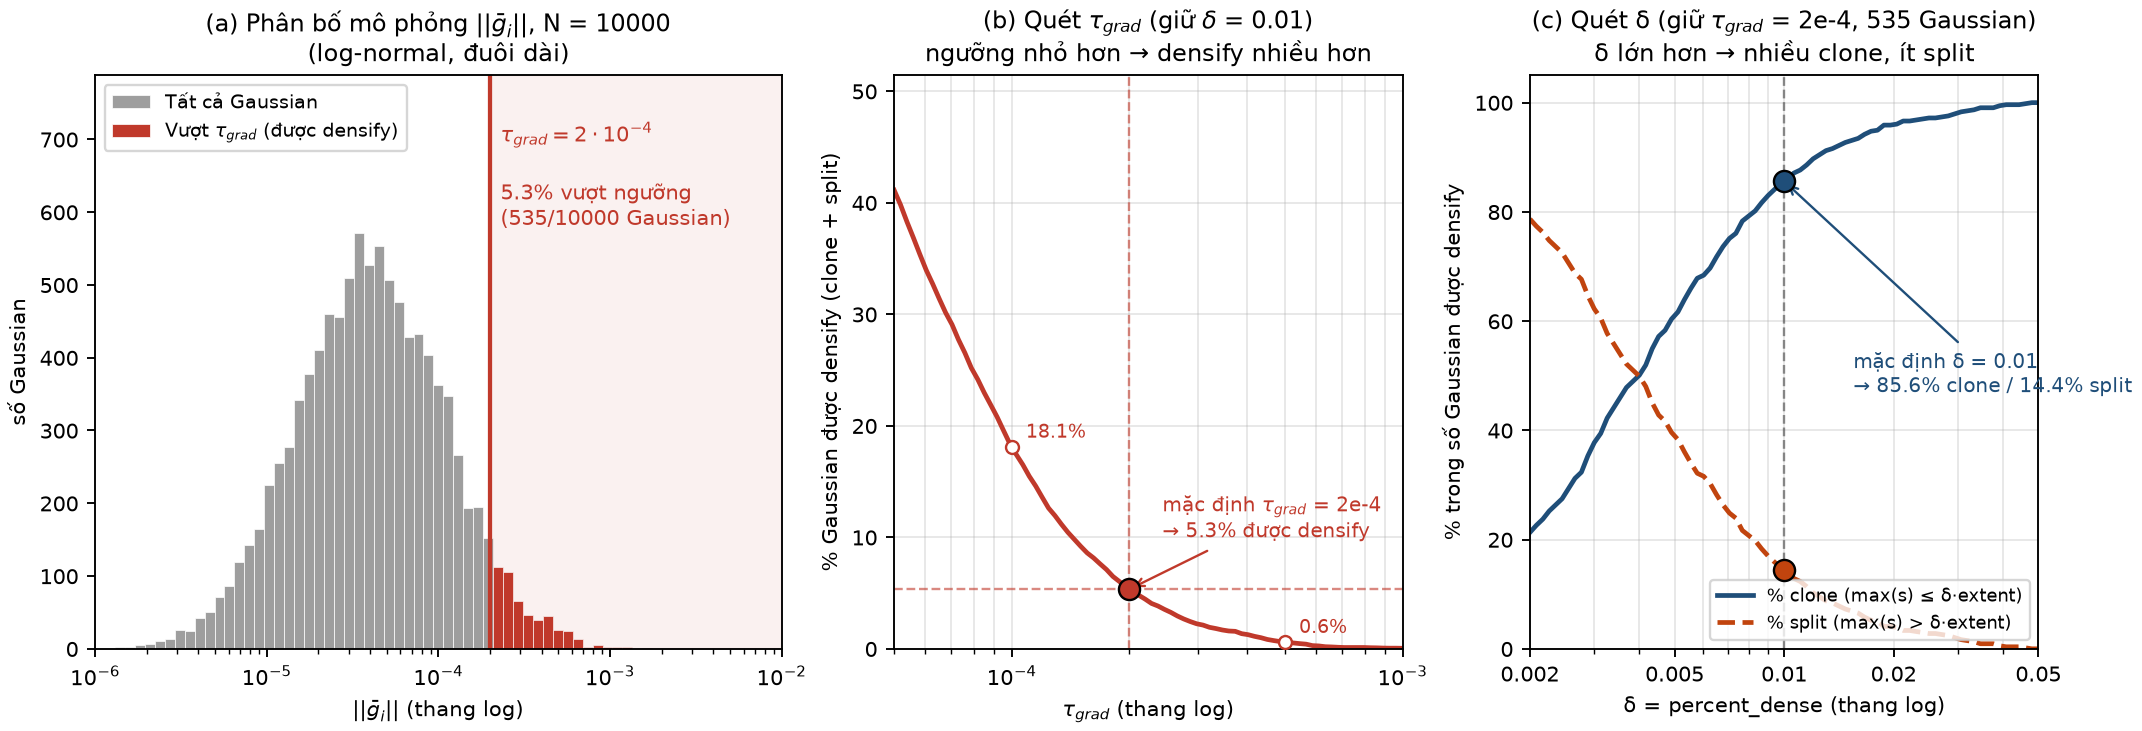
\includegraphics[width=0.85\linewidth]{fig_07_threshold_sweep.png}
\captionof{figure}{\footnotesize (a) phân bố $\|\bar g_i\|$; (b) \% densify theo $\tau_{grad}$; (c) \% clone/split theo $\delta$.}
\end{center}
\end{frame}

% --- fig_08_clone_before_after.png ---
\begin{frame}{Clone: sao chép nguyên trạng để tăng chi tiết}
\begin{columns}
\begin{column}{0.5\linewidth}
\footnotesize
\begin{itemize}
    \item Điều kiện: $\|\bar g_i\| \ge \tau_{grad}$ \textbf{và} $\max(s_i) \le \delta\cdot\text{extent}$ — Gaussian nhỏ nhưng đang dưới tái tạo (under-reconstruction).
    \item Ví dụ script: $\mu_i=(0.100,0.050)$, $s_i=(0.006,0.003)$, góc $q_i=30^\circ$, $\alpha_i=0.6$.
    \item Phép clone: $\theta_{new} = \theta_i$ — sao chép \emph{y nguyên} mọi trường ($\mu, s, q, \alpha$, hệ số SH), không đổi scale, giữ nguyên bản gốc.
    \item Hai Gaussian con trùng hoàn toàn vị trí ngay sau clone; chỉ tách ra nhờ gradient khác nhau ở các vòng tối ưu tiếp theo.
    \item Kế toán: $N: 1 \to 2$ (mỗi lần clone làm $N$ tăng đúng 1).
\end{itemize}
\end{column}
\begin{column}{0.5\linewidth}
\centering
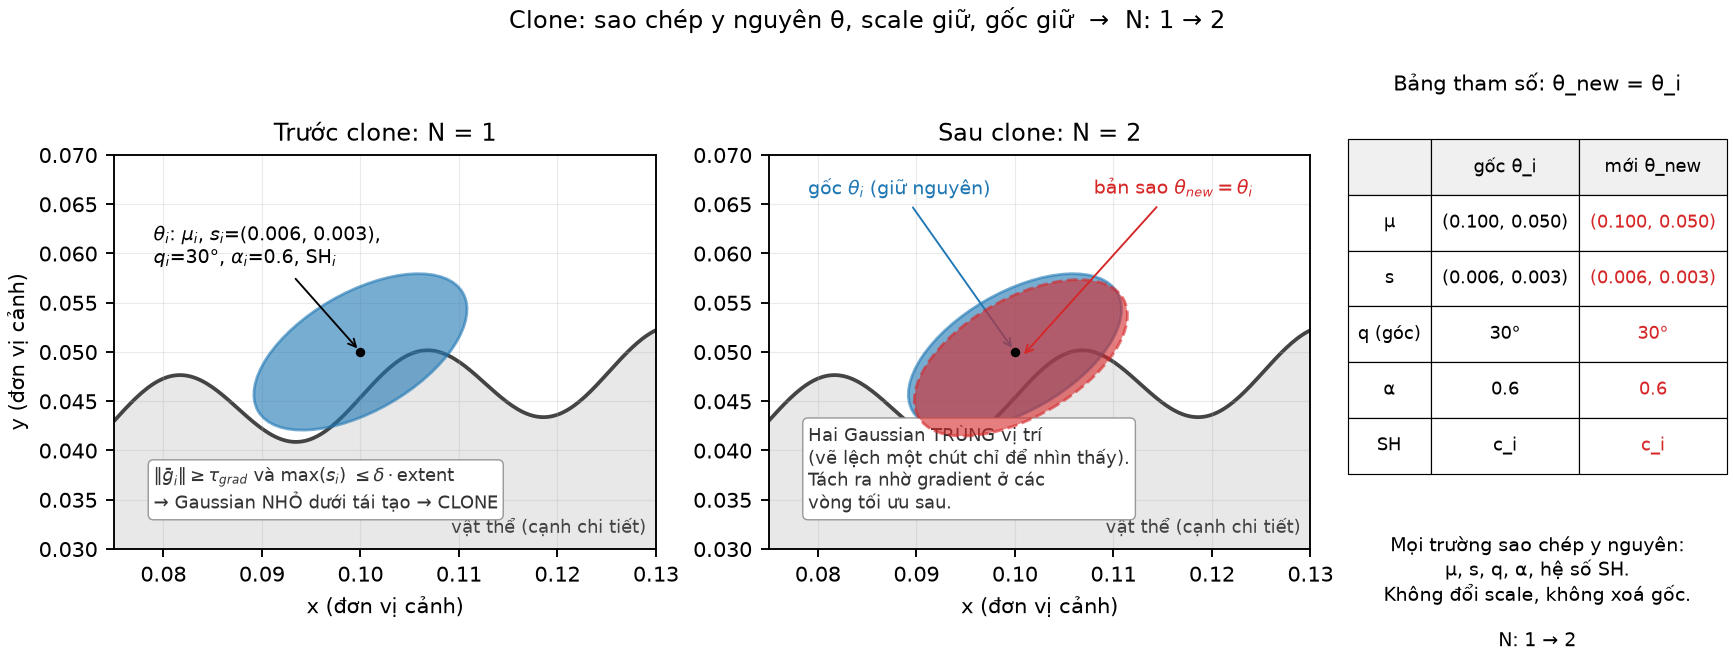
\includegraphics[width=\linewidth]{fig_08_clone_before_after.png}
\captionof{figure}{\footnotesize Trước clone ($N{=}1$) và sau clone ($N{=}2$, hai Gaussian trùng $\theta$) trên một cạnh chi tiết của vật thể.}
\end{column}
\end{columns}
\end{frame}

% --- fig_09_split_geometry.png ---
\begin{frame}{Split: hình học phân tách Gaussian quá to}
\begin{columns}
\begin{column}{0.5\linewidth}
\footnotesize
\begin{itemize}
    \item Điều kiện: $\|\bar g_i\| \ge \tau_{grad}$ \textbf{và} $\max(s_i) > \delta\cdot\text{extent}$ — Gaussian quá to đang gánh một vùng có nhiều chi tiết.
    \item Sinh 2 mẫu cục bộ $e^{(j)} \sim \mathcal{N}(0,\operatorname{diag}(s_i^2))$, $j=1,2$, rồi xoay về hệ toạ độ thế giới:
    \[
    \mu^{(j)} = \mu_i + R(q_i)\,e^{(j)}, \qquad s^{(j)} = s_i / 1.6,\quad q^{(j)}=q_i
    \]
    \item Ví dụ script: $s_i=(0.06,0.02)$, $q_i=40^\circ$ $\Rightarrow$ $s^{(j)}=(0.0375,0.0125)$; hệ số chia $\texttt{SPLIT\_FACTOR}=1.6$ (diện tích mỗi con còn $1/1.6^2\approx0.39$ lần gốc).
    \item Gaussian gốc $\theta_i$ bị \textbf{xoá} sau split; $\alpha^{(j)}=\alpha_i$, SH$^{(j)}=$SH$_i$ giữ nguyên.
    \item Kế toán: $+2$ con, $-1$ gốc $\Rightarrow$ ròng $N: 1 \to 2$ (+1) mỗi Gaussian bị tách.
\end{itemize}
\end{column}
\begin{column}{0.5\linewidth}
\centering
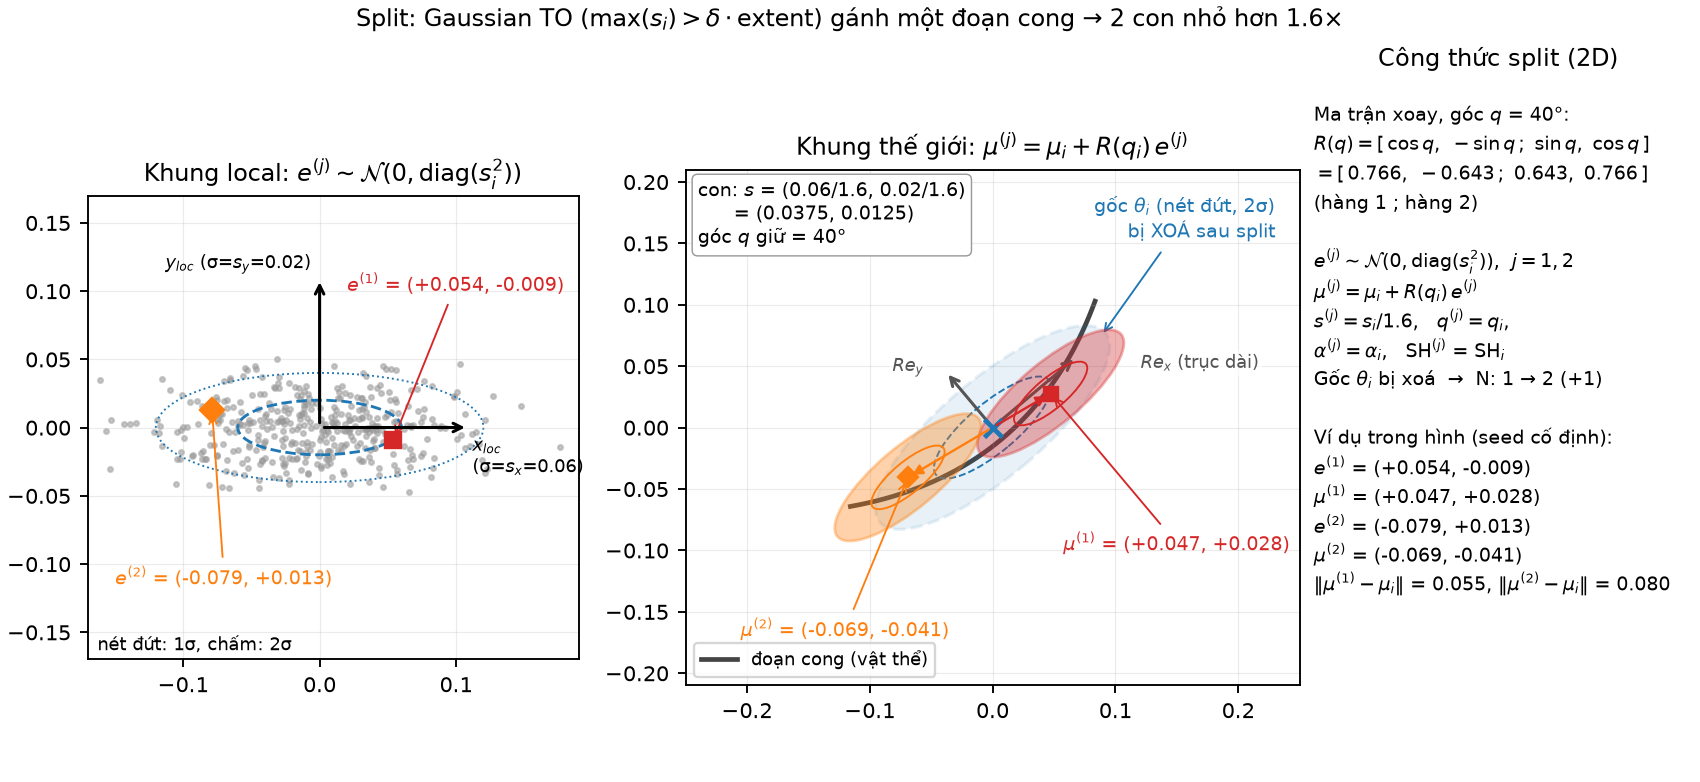
\includegraphics[width=\linewidth]{fig_09_split_geometry.png}
\captionof{figure}{\footnotesize Trái: mẫu $e^{(j)}$ trong hệ local; giữa: $\mu^{(j)}=\mu_i+R(q_i)e^{(j)}$ trong hệ world với 2 con nhỏ hơn 1.6 lần; phải: công thức và số liệu ví dụ.}
\end{column}
\end{columns}
\end{frame}

% =============================================================
% ADC-TLb: Adaptive Density Control -- Prune theo tiêu chí + Opacity reset
% Tiếp nối ADC-TLa (clone/split). 9 frame, dùng ảnh trong figures/.
% =============================================================

% --- fig_10_split_samples.png ---
\begin{frame}{Split: mẫu Monte Carlo vị trí con quanh gốc}
\begin{columns}[T]
\begin{column}{0.46\linewidth}
\footnotesize
\begin{itemize}
  \item Gaussian gốc: $s_i = (0.06, 0.02)$, góc xoay $40^\circ$, mô phỏng $2000$ cặp con (seed cố định).
  \item Vị trí con lấy mẫu: $e^{(j)} \sim \mathcal{N}(0, \mathrm{diag}(s_i^2))$ trong khung cục bộ, rồi xoay về khung thế giới: $\mu^{(j)} - \mu_i = R\, e^{(j)}$.
  \item Độ lệch chuẩn mẫu đo được: theo trục dài $\approx 0.06$ (lý thuyết $0.06$), theo trục ngắn $\approx 0.02$ (lý thuyết $0.02$) -- khớp covariance gốc.
  \item Khoảng cách chuẩn hoá $\|\mu^{(j)}-\mu_i\|/\max(s_i)$: trung vị $\approx 1{,}0$, khoảng $90\%$ số con nằm trong bán kính này.
  \item Diện tích ellipse mỗi con co lại $1/1.6^2 = 0{,}391$ lần gốc; hai con cộng lại $2/1.6^2 = 0{,}781$ lần gốc (thể tích 3D co $1.6^3 \approx 4{,}1\times$).
\end{itemize}
\end{column}
\begin{column}{0.5\linewidth}
\centering
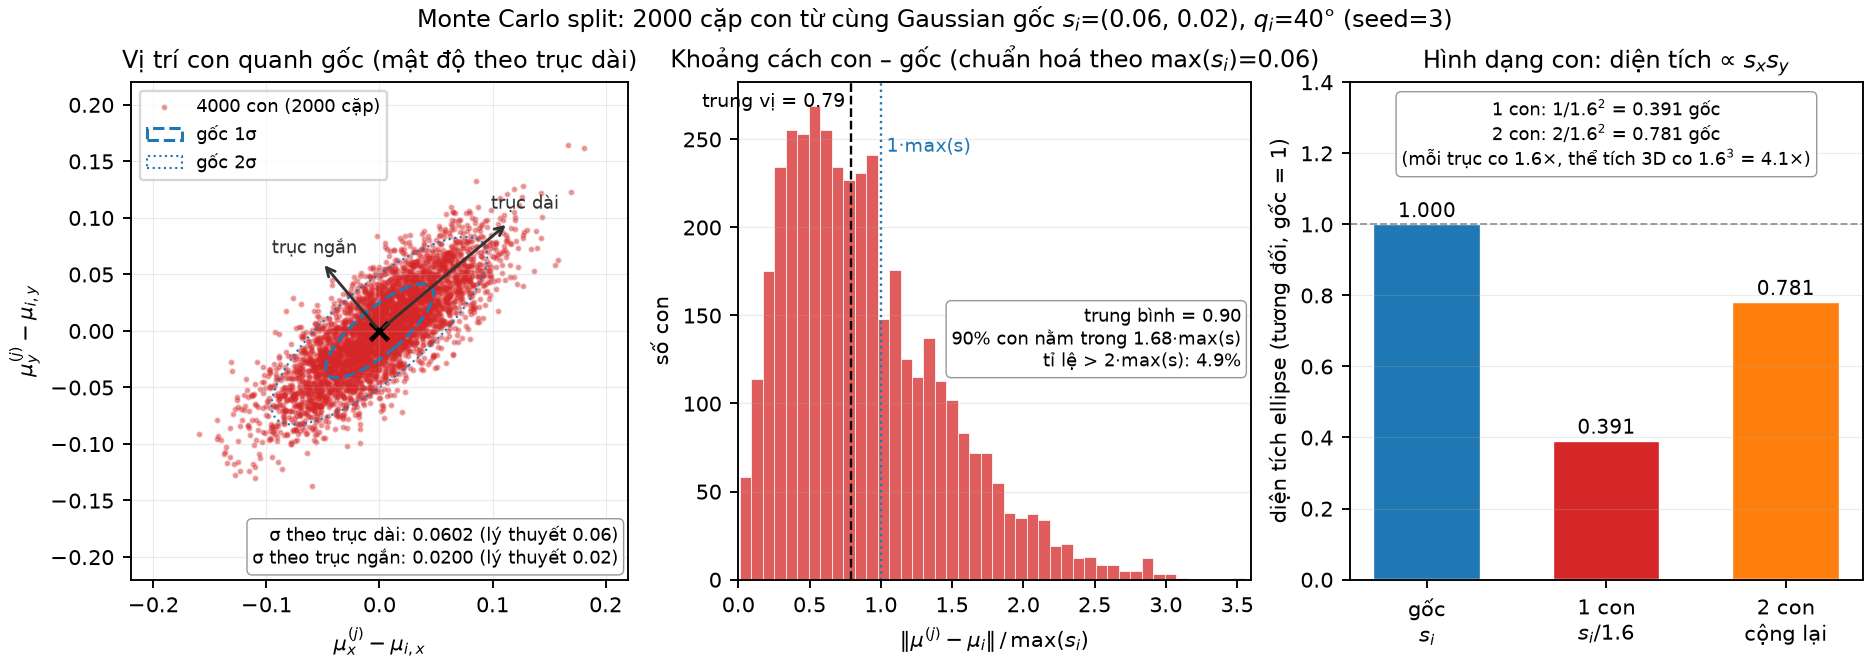
\includegraphics[width=0.95\linewidth]{fig_10_split_samples.png}
\captionof{figure}{\footnotesize Scatter $2000$ cặp con quanh Gaussian gốc, histogram khoảng cách chuẩn hoá, và so sánh diện tích ellipse gốc/con.}
\end{column}
\end{columns}
\end{frame}

% --- fig_11_N_accounting.png ---
\begin{frame}{Kế toán số Gaussian $N$ qua một bước densify + prune}
\footnotesize
\begin{itemize}
  \item Trong một bước densify+prune: $N_{\text{old}} = 1000$, clone thêm $n_{\text{clone}} = 120$, split $n_{\text{split}} = 80$ Gaussian (mỗi Gaussian split sinh $2$ con, xoá $1$ gốc $\Rightarrow$ ròng $+n_{\text{split}}$), prune xoá $n_{\text{prune}} = 45$.
  \[ N_{t+1} = N_t + n_{\text{clone}} + n_{\text{split}} - n_{\text{prune}} = 1000 + 120 + 80 - 45 = 1155 \]
  \item Nếu tỉ lệ densify không đổi mỗi bước, $N$ tăng theo cấp số nhân: $N(t) = N_0(1+r)^t$ với $r \approx 1{,}5\%$ mỗi $100$ vòng, so với tăng tuyến tính $N_0(1 + rt)$.
  \item Với $N_0 = 100\,000$ và $144$ bước densify (mỗi $100$ vòng, từ vòng $500$ đến $15000$): luỹ thừa cho $N \approx 8{,}2\times N_0$ tại $t=144$, trong khi tuyến tính chỉ $\approx 3{,}16\times N_0$.
  \item Đây là lý do cần các tiêu chí prune \emph{cứng} và tần suất reset opacity đều đặn -- nếu không, số Gaussian sẽ bùng nổ và vượt ngân sách bộ nhớ/tốc độ render.
\end{itemize}
\centering
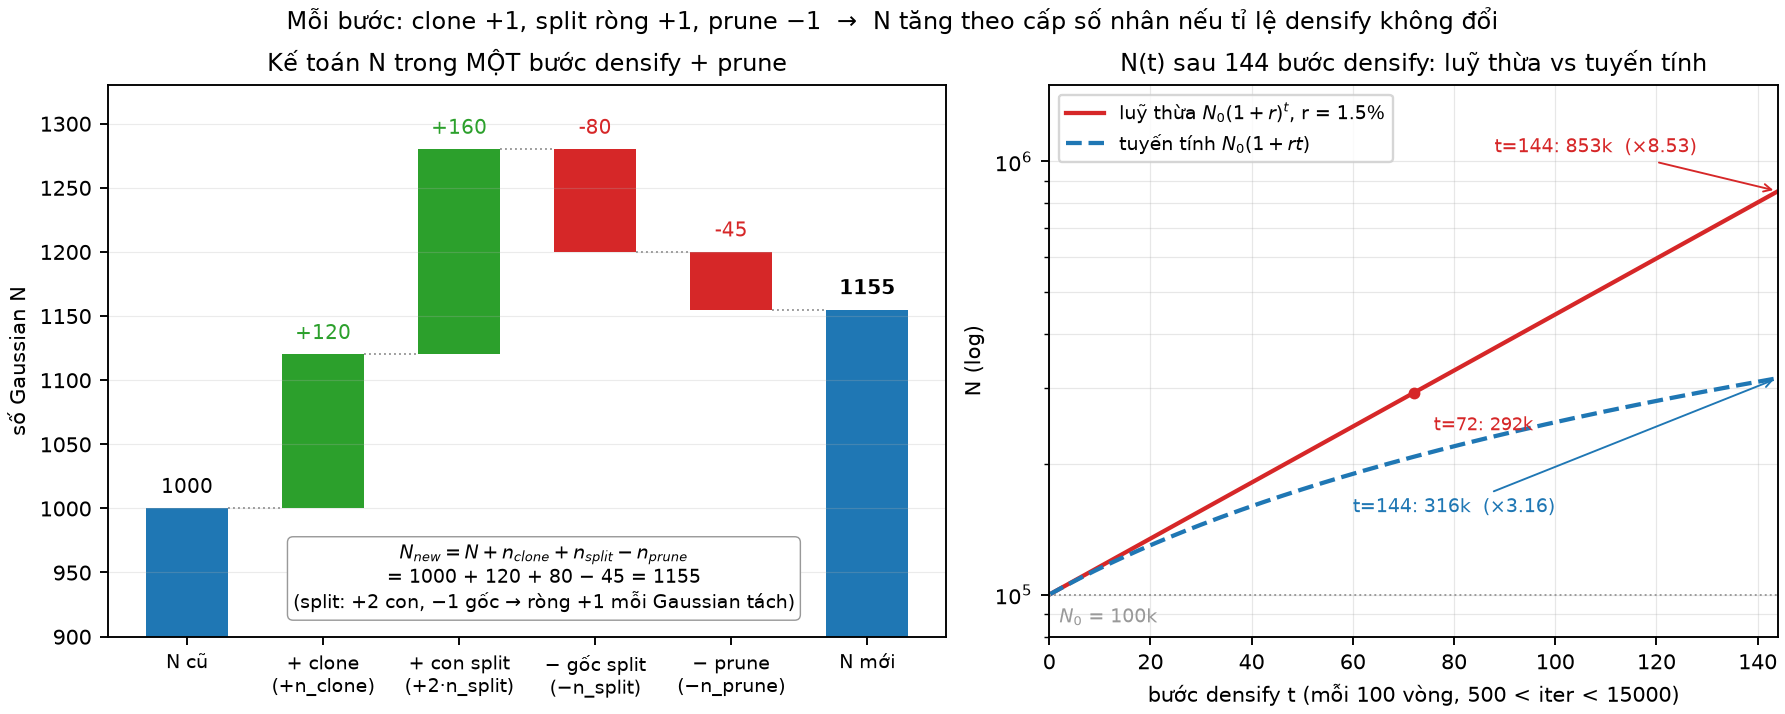
\includegraphics[width=0.72\linewidth]{fig_11_N_accounting.png}
\captionof{figure}{\footnotesize Waterfall kế toán $N$ trong một bước, và tăng trưởng $N(t)$ luỹ thừa vs.\ tuyến tính qua $144$ bước.}
\end{frame}

% --- fig_12_prune_alpha.png ---
\begin{frame}{Tiêu chí prune 1: opacity thấp $\alpha_i < 0{,}005$}
\begin{columns}[T]
\begin{column}{0.48\linewidth}
\footnotesize
\begin{itemize}
  \item Điều kiện xoá: $\alpha_i < 0{,}005$ (ngưỡng \texttt{min\_opacity} mặc định Inria).
  \item Ý nghĩa vật lý: Gaussian gần như trong suốt hoàn toàn -- đóng góp không đáng kể vào công thức alpha-blending của ảnh render, giữ lại chỉ tốn tài nguyên vô ích.
  \item Trên quần thể mô phỏng $N = 20\,000$ Gaussian (trộn opacity từ nhiều nguồn: đa số hữu ích, một cụm nhỏ vừa reset, một số trung gian): số Gaussian bị xoá là $981/20\,000 \approx 4{,}91\%$.
  \item Phân phối $\alpha$ có một cụm nhỏ dồn sát $0$ (Gaussian vừa reset opacity chưa kịp "hồi") -- đây chính là nhóm bị prune ngay ở lần densify kế tiếp nếu không tăng $\alpha$ kịp.
\end{itemize}
\end{column}
\begin{column}{0.5\linewidth}
\centering
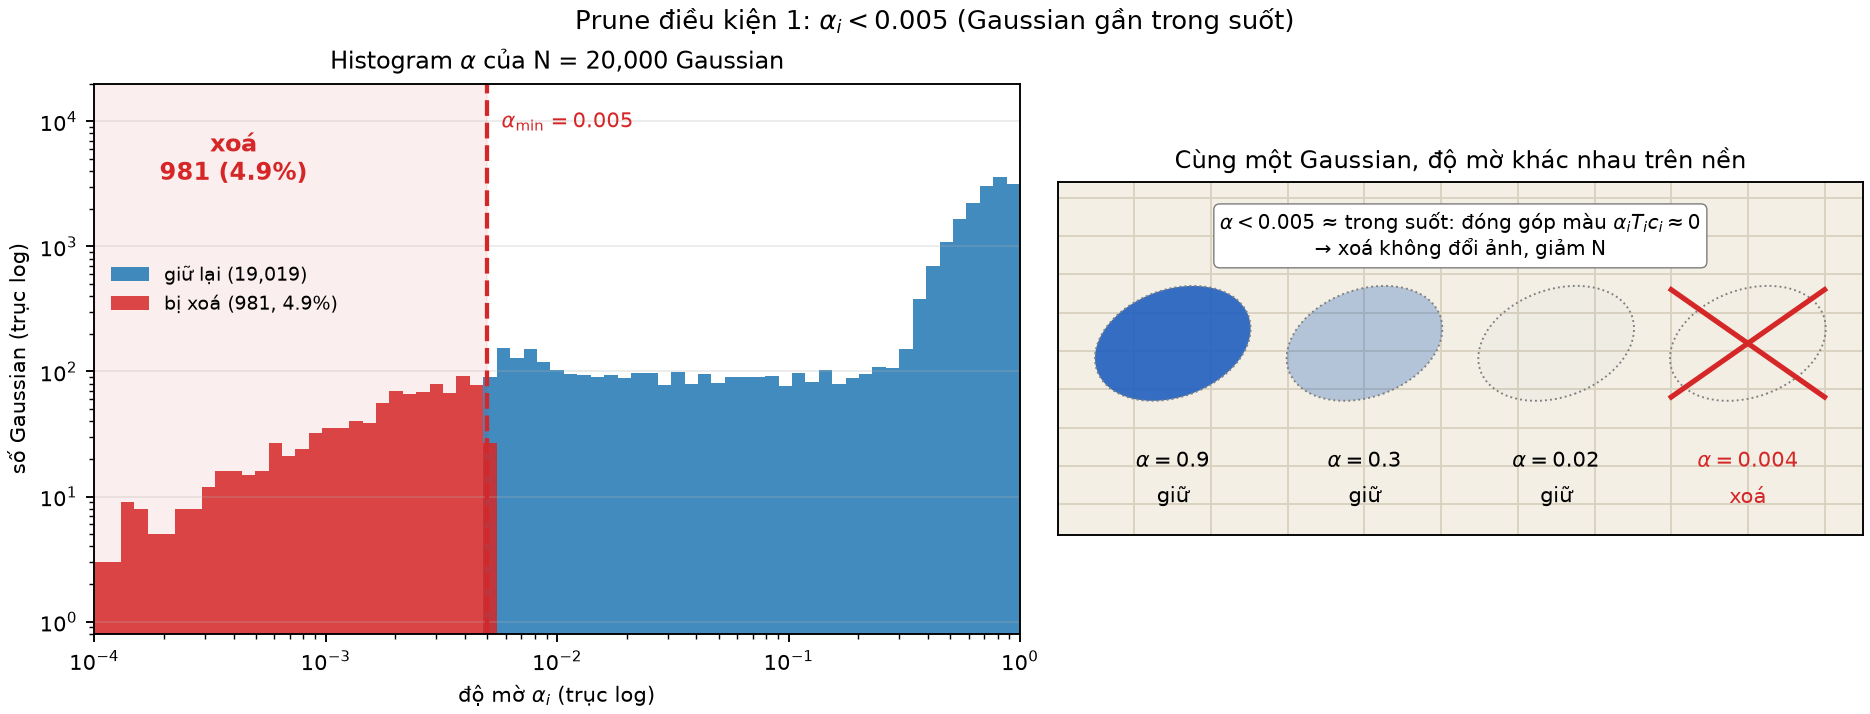
\includegraphics[width=0.95\linewidth]{fig_12_prune_alpha.png}
\captionof{figure}{\footnotesize Histogram $\alpha$ (trục log) với vùng xoá $\alpha<0{,}005$ tô đỏ; $981/20\,000 \approx 4{,}91\%$ Gaussian bị xoá.}
\end{column}
\end{columns}
\end{frame}

% --- fig_13_prune_radius2d.png ---
\begin{frame}{Tiêu chí prune 2: bán kính chiếu 2D $r_i^{2D} > 20$ px}
\footnotesize
\begin{itemize}
  \item Xấp xỉ hình học: $r^{2D} \approx \dfrac{f \cdot s}{z}$, với $f$ là tiêu cự (px), $s$ là scale 3D, $z$ là độ sâu tới camera.
  \item Ngưỡng Inria: xoá nếu $r_i^{2D} > 20$ px, nhưng \textbf{chỉ áp dụng khi $t > 3000$} (sau lần reset opacity đầu tiên); trước đó điều kiện này bị bỏ qua để không xoá nhầm Gaussian to đang hình thành.
  \item \texttt{max\_radii2D} là giá trị lớn nhất quan sát được qua mọi view đã render, cập nhật mỗi vòng bởi rasterizer.
  \item Ví dụ số: $s=0{,}01, z=1, f=1000 \Rightarrow r^{2D}=10$ px (giữ); $s=0{,}03, z=1 \Rightarrow r^{2D}=30$ px (xoá); nhưng cùng $s=0{,}03$ với $z=3 \Rightarrow r^{2D}=10$ px (giữ) -- cùng một scale 3D có thể giữ hoặc xoá tuỳ độ sâu.
  \item Cùng một $s$ lớn, gần camera cho $r^{2D}$ lớn hơn xa camera -- đây là lý do tiêu chí này bổ sung cho tiêu chí scale tuyệt đối (không phụ thuộc view).
\end{itemize}
\centering
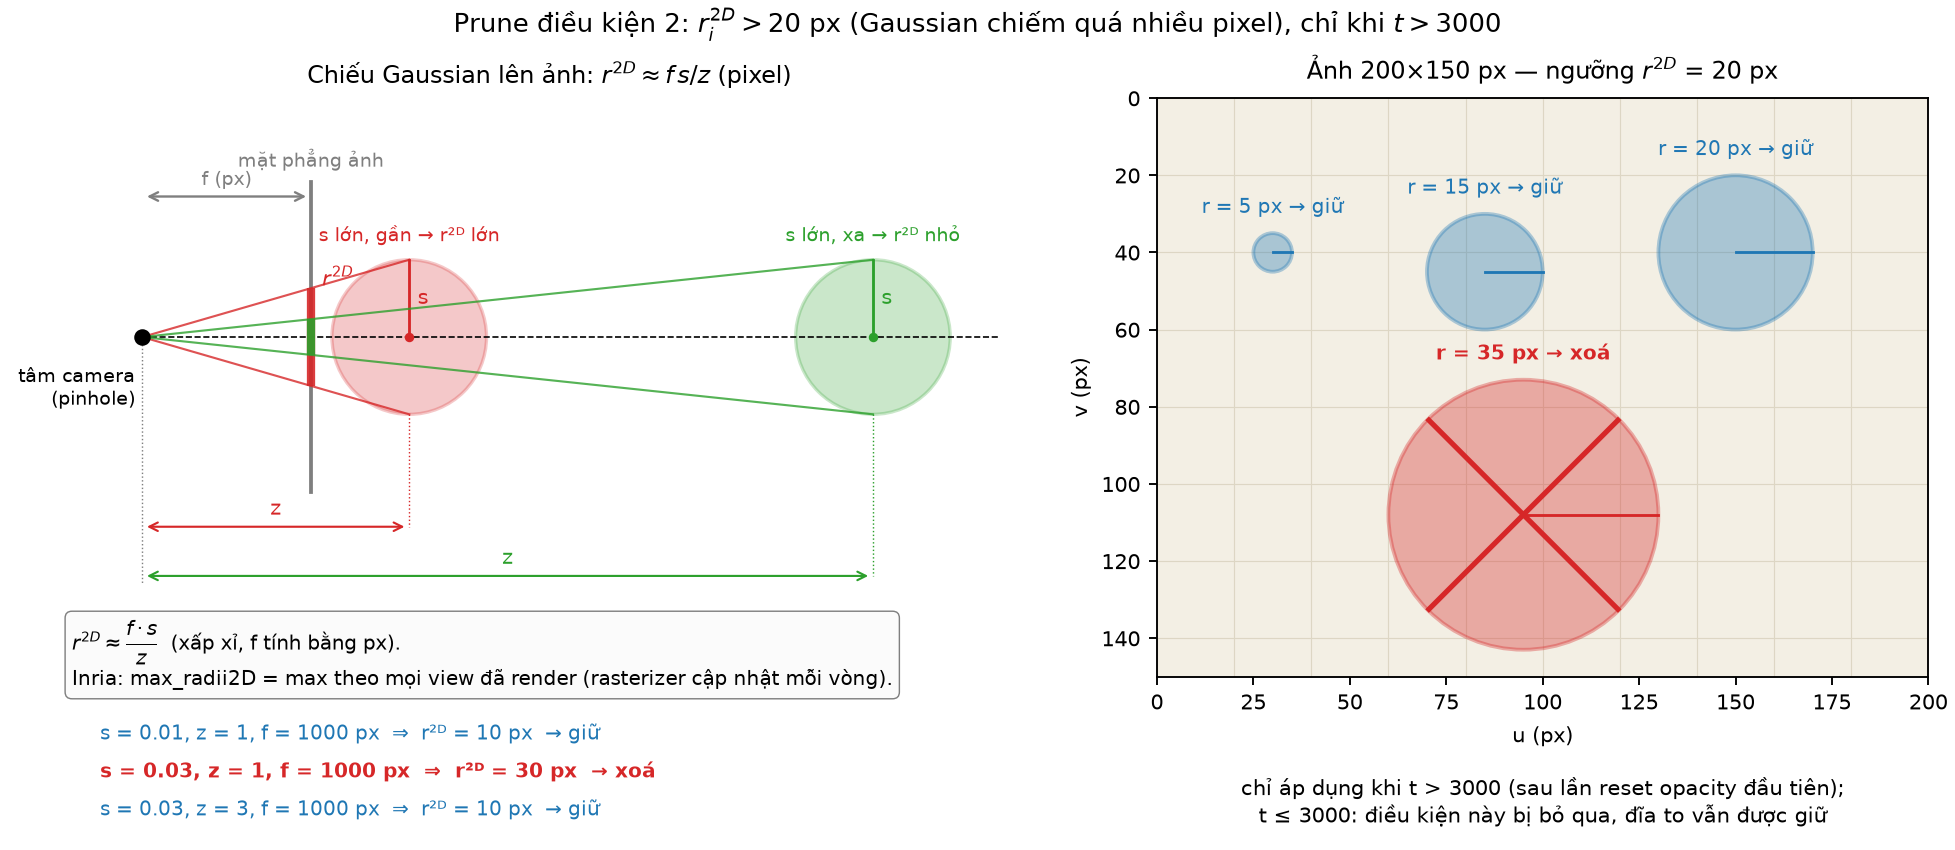
\includegraphics[width=0.7\linewidth]{fig_13_prune_radius2d.png}
\captionof{figure}{\footnotesize Sơ đồ chiếu pinhole $r^{2D}\approx fs/z$ và ảnh minh hoạ các đĩa với ngưỡng $20$ px.}
\end{frame}

% --- fig_14_prune_scale.png ---
\begin{frame}{Tiêu chí prune 3: scale tuyệt đối $\max(s_i) > 0{,}1 \cdot \text{extent}$}
\footnotesize
\begin{itemize}
  \item Điều kiện xoá: bán trục lớn nhất của Gaussian vượt quá $10\%$ kích thước cảnh (\texttt{extent}, world-space, không phụ thuộc camera).
  \item Diễn giải: Gaussian với $\max(s_i)/\text{extent} > 0{,}1$ phủ lên quá nhiều vật thể khác nhau trong cảnh -- thường là artefact "sương"/floater to, không mô tả bề mặt cụ thể nào $\Rightarrow$ xoá ngay bất kể $\alpha$ hay gradient.
  \item Ví dụ minh hoạ với $4$ Gaussian có $\max(s)/\text{extent} \in \{0{,}02,\ 0{,}05,\ 0{,}10,\ 0{,}18\}$: chỉ hai Gaussian đầu ($0{,}02$ và $0{,}05$) được giữ; $0{,}10$ và $0{,}18$ bị xoá (ranh giới $0{,}10$ tính là vượt).
  \item So sánh: ngưỡng khởi tạo split/clone dùng $\delta = 0{,}01 \cdot \text{extent}$ -- nhỏ hơn ngưỡng prune này $10$ lần, cho thấy hai cơ chế nhắm hai thái cực kích thước khác nhau.
\end{itemize}
\centering
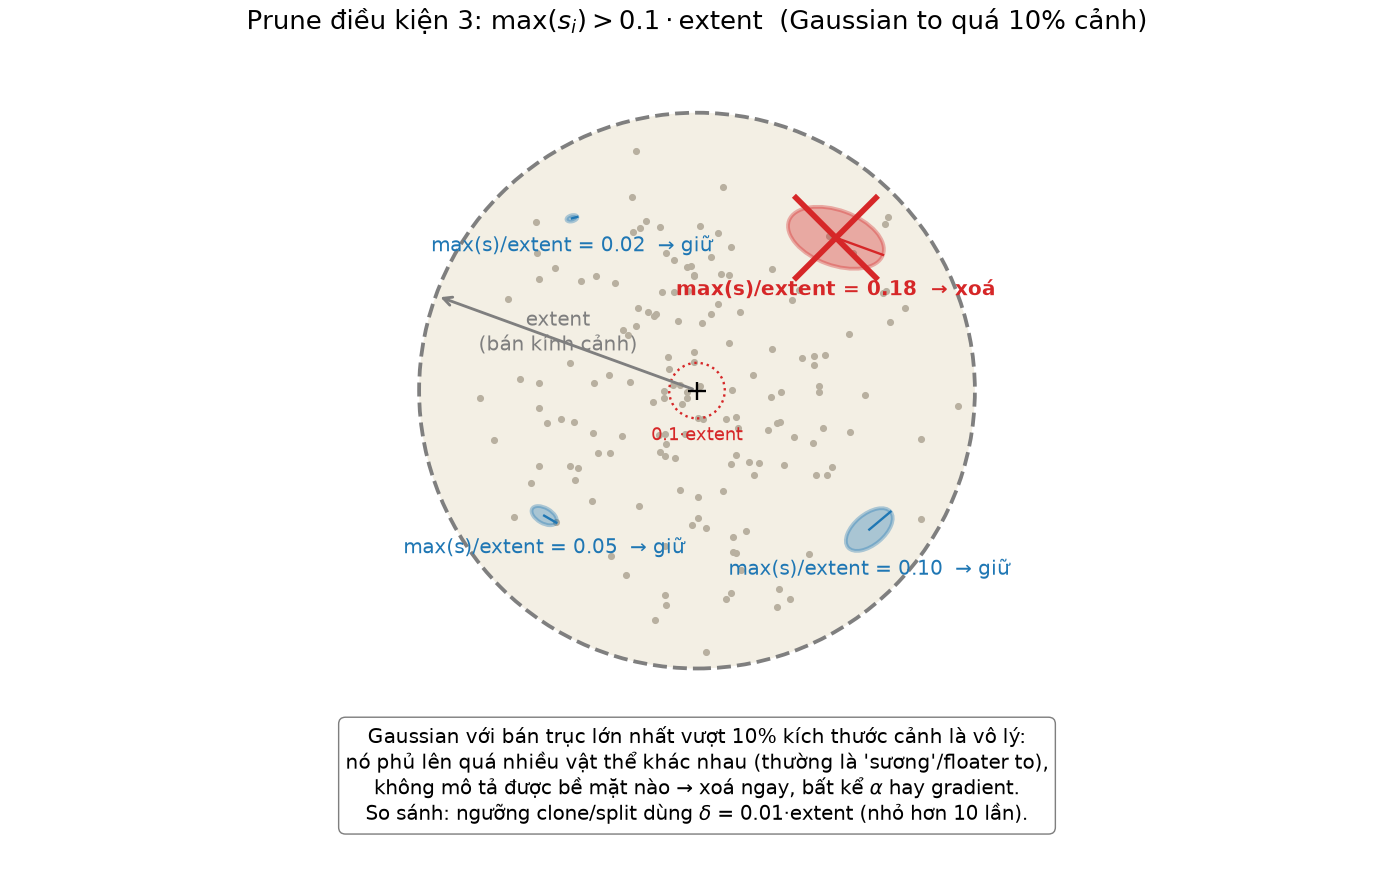
\includegraphics[width=0.6\linewidth]{fig_14_prune_scale.png}
\captionof{figure}{\footnotesize Vòng tròn extent cảnh và các Gaussian mẫu ở nhiều tỉ lệ $\max(s)/\text{extent}$, đánh dấu xoá/giữ.}
\end{frame}

% --- fig_15_prune_or_region.png ---
\begin{frame}{Kết hợp tiêu chí prune bằng phép OR}
\footnotesize
\[
\mathrm{xoa}_i = \big[\alpha_i < 0{,}005\big] \;\vee\; \big[r_i^{2D} > 20\text{ px},\; t>3000\big] \;\vee\; \big[\max(s_i) > 0{,}1\cdot\text{extent}\big]
\]
\begin{itemize}
  \item Gaussian chỉ cần vi phạm \textbf{một} trong ba điều kiện (A: $\alpha$ thấp, B: bán kính 2D lớn, C: scale tuyệt đối lớn) là bị xoá -- vùng quyết định trong không gian tham số là \emph{hợp} $A \cup B \cup C$.
  \item Trên $N=20\,000$ Gaussian mô phỏng, tại $t=9000$ (đủ cả 3 điều kiện, $|A|=981$, $|B|=1869$, $|C|=237$): tổng vùng hợp $|A\cup B\cup C| = 2751$ Gaussian bị xoá ($\approx 13{,}8\%$).
  \item Tại $t=2000$ ($t \le 3000$ nên điều kiện B bị bỏ qua): chỉ còn $A$ và $C$ hoạt động, tổng xoá $= 1204$ Gaussian ($\approx 6{,}0\%$) -- thấp hơn hẳn vì thiếu tiêu chí B.
  \item Tổng OR luôn nhỏ hơn $|A|+|B|+|C|$ vì các điều kiện chồng lấn nhau (ví dụ Gaussian to thường cũng mờ do "sương" -- vùng $A\cap C$ khác rỗng).
  \item Đây là prune \emph{cứng}: xoá ngay lập tức, không cần ứng viên hay ngân sách như trong densify.
\end{itemize}
\centering
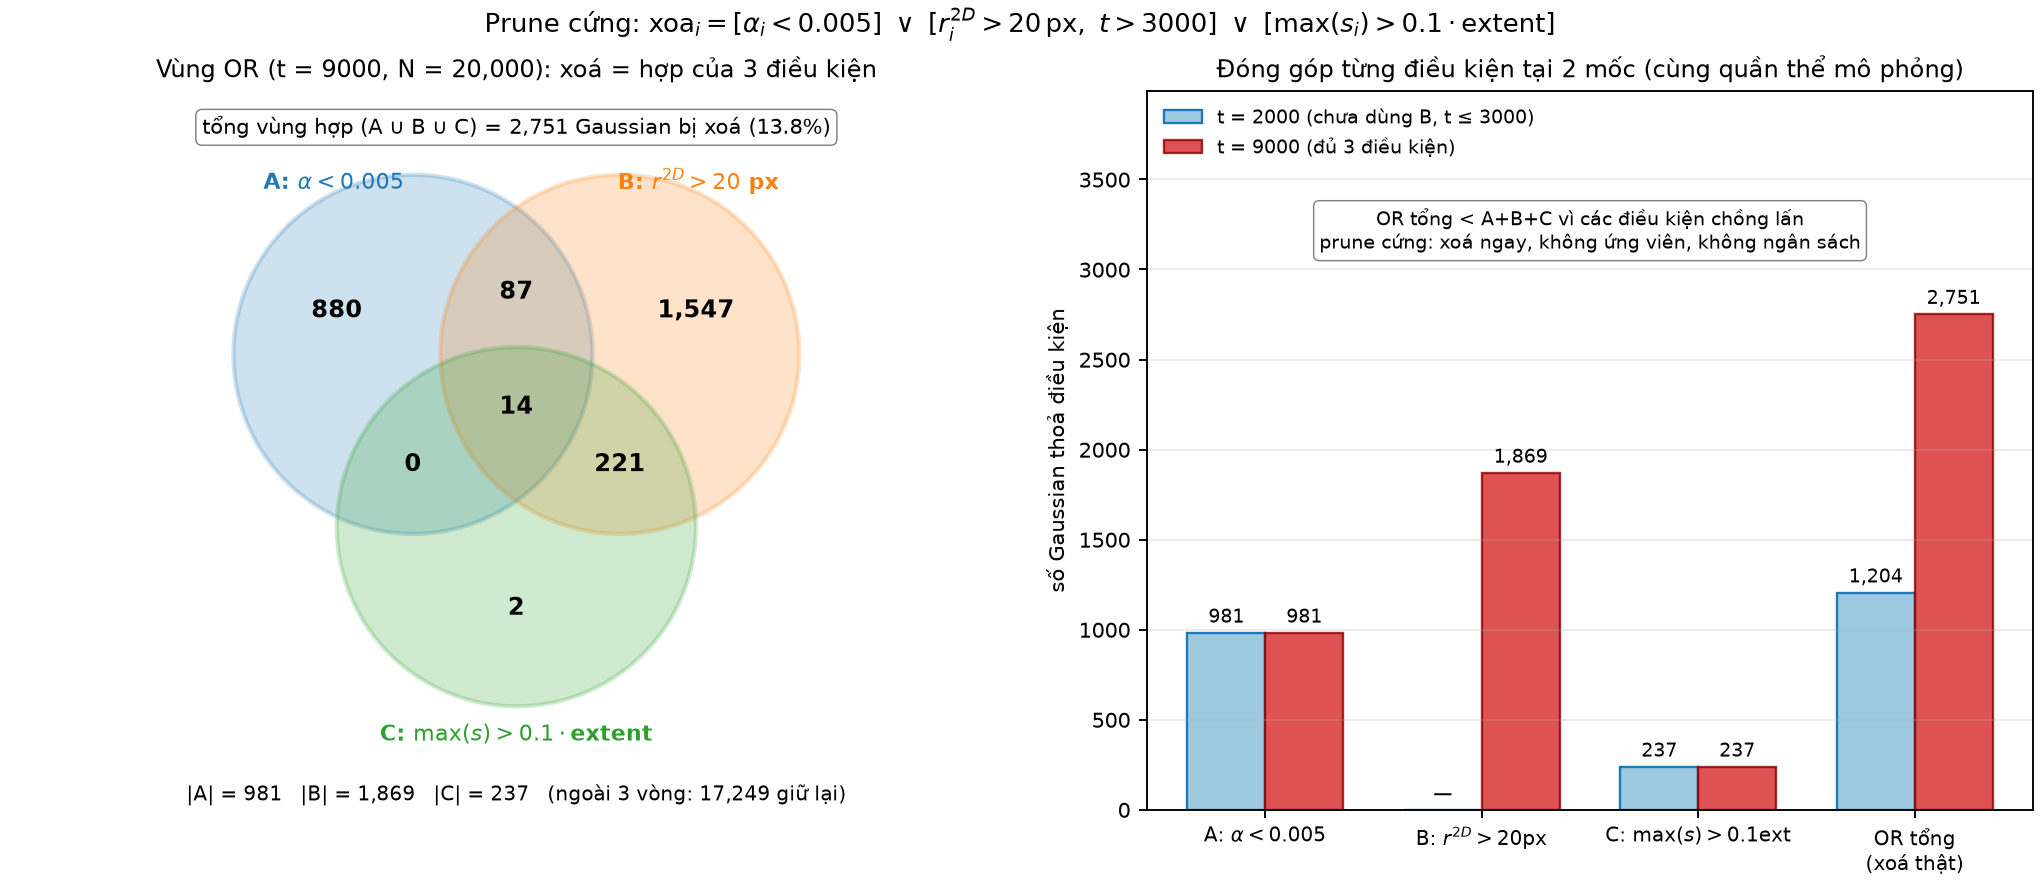
\includegraphics[width=0.62\linewidth]{fig_15_prune_or_region.png}
\captionof{figure}{\footnotesize Sơ đồ Venn 3 vòng và bar chart so sánh đóng góp từng tiêu chí tại $t=2000$ và $t=9000$.}
\end{frame}

% --- fig_16_sigmoid_inverse.png ---
\begin{frame}{Vì sao lưu opacity dưới dạng logit: sigmoid và nghịch đảo}
\begin{columns}[T]
\begin{column}{0.5\textwidth}
\scriptsize
\begin{itemize}
  \item $\alpha{\in}[0,1]$ tham số hoá gián tiếp qua $x{\in}\mathbb{R}$ (không chặn):
  $\alpha{=}\sigma(x){=}\frac{1}{1+e^{-x}}$, $x{=}\sigma^{-1}(\alpha){=}\ln\frac{\alpha}{1-\alpha}$.
  \item Tối ưu $x$ bằng GD không ràng buộc, $\alpha{=}\sigma(x)$ tự động $\in[0,1]$.
  \item Mốc: $\alpha{=}0.005\Leftrightarrow x{\approx}{-}5.293$; $\alpha{=}0.01\Leftrightarrow x{\approx}{-}4.595$; $\alpha{=}0.99\Leftrightarrow x{\approx}{+}4.595$.
  \item Reset: $\alpha_{\text{sau}}{=}\min(\alpha_{\text{trước}},0.01)$, rồi $x{\leftarrow}\sigma^{-1}(\alpha_{\text{sau}})$.
\end{itemize}
\end{column}
\begin{column}{0.5\textwidth}
\centering
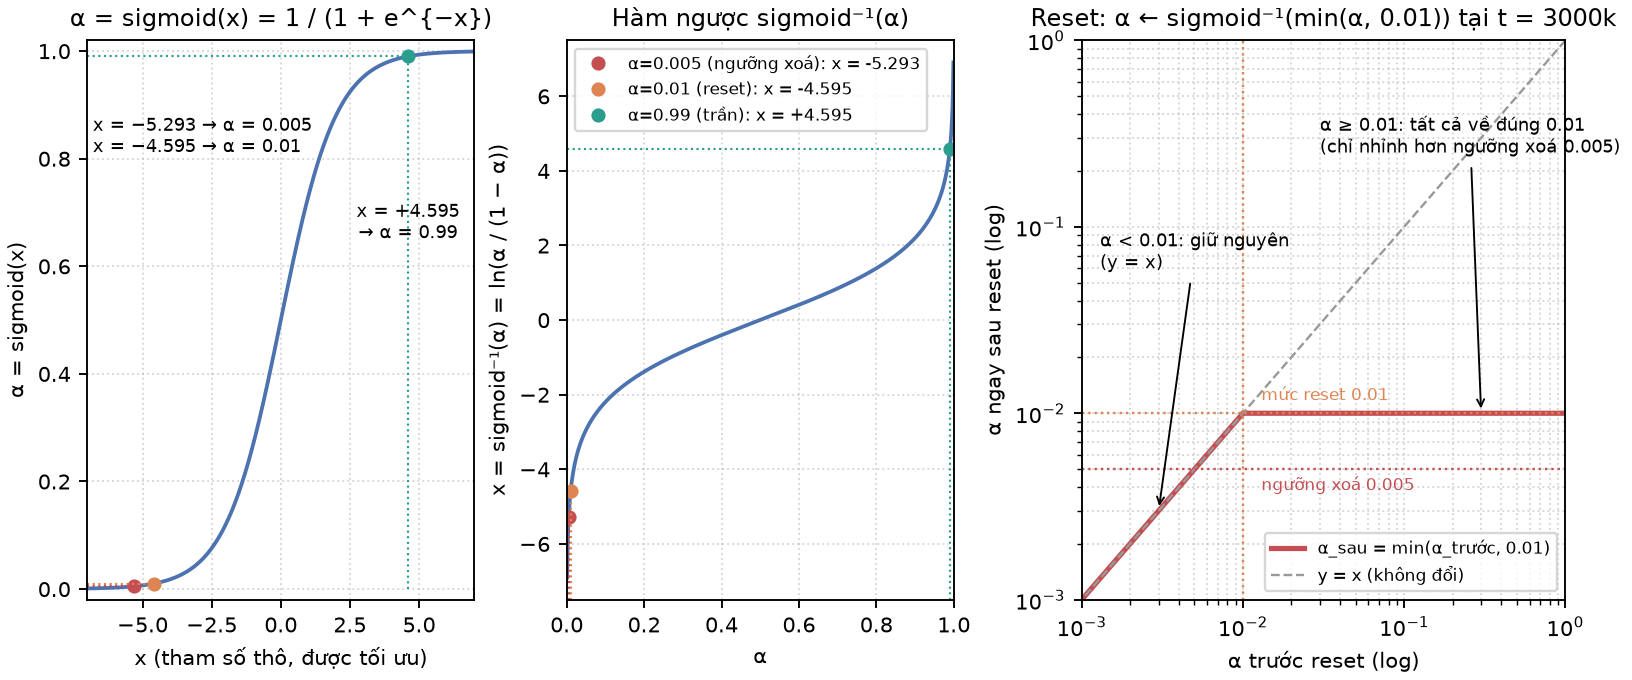
\includegraphics[width=0.95\linewidth]{fig_16_sigmoid_inverse.png}
\captionof{figure}{\footnotesize $\sigma(x)$, $\sigma^{-1}(\alpha)$, ánh xạ reset.}
\end{column}
\end{columns}
\end{frame}

% --- fig_17_opacity_trajectory.png ---
\begin{frame}{Quỹ đạo opacity theo thời gian: nhảy xuống rồi phục hồi}
\footnotesize
\begin{itemize}
  \item Mô phỏng $4$ Gaussian qua $4$ lần reset tại $t \in \{3000, 6000, 9000, 12000\}$, khởi tạo $\alpha_0 = 0{,}1$ (giá trị khởi tạo mặc định Inria).
  \item (i) Gaussian hữu ích: hồi phục nhanh về $\approx 0{,}9$ sau mỗi lần reset (tốc độ hồi phục cao).
  \item (ii) Gaussian "ảo"/thừa: sau lần reset tại $t=6000$ không hồi phục được nữa (gradient không đủ mạnh), $\alpha$ giảm dần và bị prune ngay khi chạm ngưỡng $\alpha < 0{,}005$ tại lần densify kế tiếp.
  \item (iii) Gaussian hữu ích vừa: hồi phục chậm hơn, chỉ về $\approx 0{,}4$.
  \item (iv) Gaussian mới sinh (do clone/split) tại $t=9000$ với $\alpha_0=0{,}1$ -- tham gia chu trình reset từ mốc $t=12000$ trở đi.
  \item Mỗi lần reset là một "cú nhảy xuống" tức thời về $\alpha=0{,}01$ trên trục log, sau đó quỹ đạo phân nhánh: hoặc leo trở lại (hữu ích) hoặc tụt xuống dưới ngưỡng xoá (vô dụng).
\end{itemize}
\centering
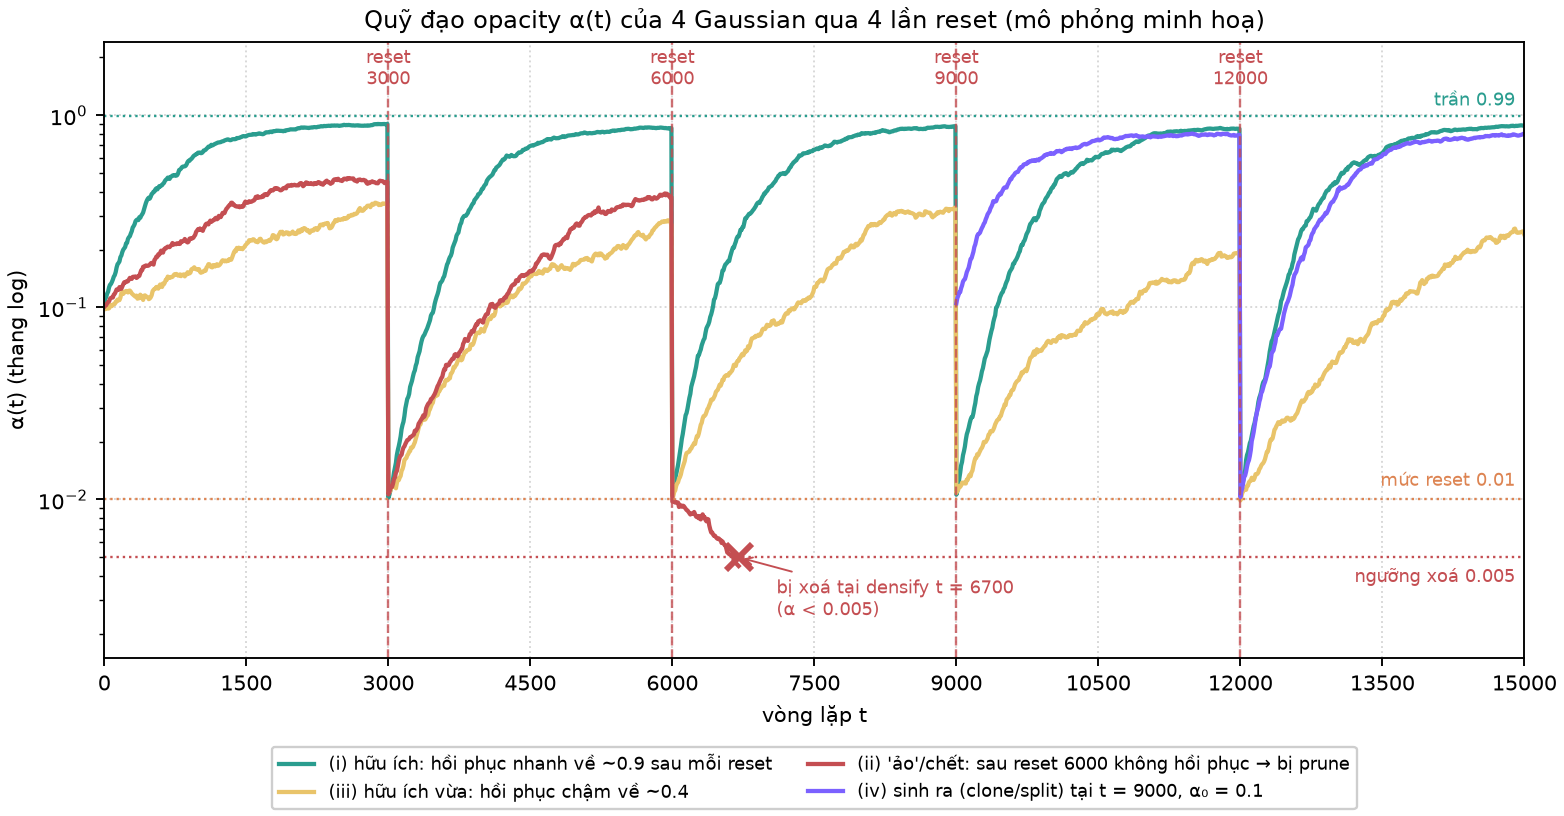
\includegraphics[width=0.68\linewidth]{fig_17_opacity_trajectory.png}
\captionof{figure}{\footnotesize $\alpha(t)$ của 4 Gaussian (thang log) qua 4 lần reset; đường (ii) bị xoá sau khi không phục hồi.}
\end{frame}

% --- fig_18_hist_reset.png ---
\begin{frame}{Toàn cảnh: histogram opacity trước/sau một lần reset}
\scriptsize
\begin{itemize}
  \item Mô phỏng $N{=}20{,}000$ quanh reset $t{=}6000$: $72\%$ "hữu ích" ($\alpha{\approx}0.80$ trước reset), $28\%$ "vô dụng" ($\alpha{\approx}0.15$).
  \item \textbf{Trước reset}: phân phối trải rộng, một lượng nhỏ đã dưới ngưỡng xoá $0.005$.
  \item \textbf{Sau reset}: $\alpha{\leftarrow}\min(\alpha,0.01)$ toàn bộ — gần như mọi Gaussian dồn về $0.01$.
  \item \textbf{500 vòng sau}: nhóm hữu ích hồi phục mạnh ($\alpha{>}0.5$), nhóm vô dụng tiếp tục giảm — một phần rơi dưới $0.005 \Rightarrow$ bị prune; $12\%$ nhóm vô dụng hồi phục vừa phải và được giữ lại.
  \item[$\Rightarrow$] Cơ chế cốt lõi: buộc mọi Gaussian "chứng minh lại" giá trị qua gradient — khép lại chu trình ADC theo thời gian.
\end{itemize}
\centering
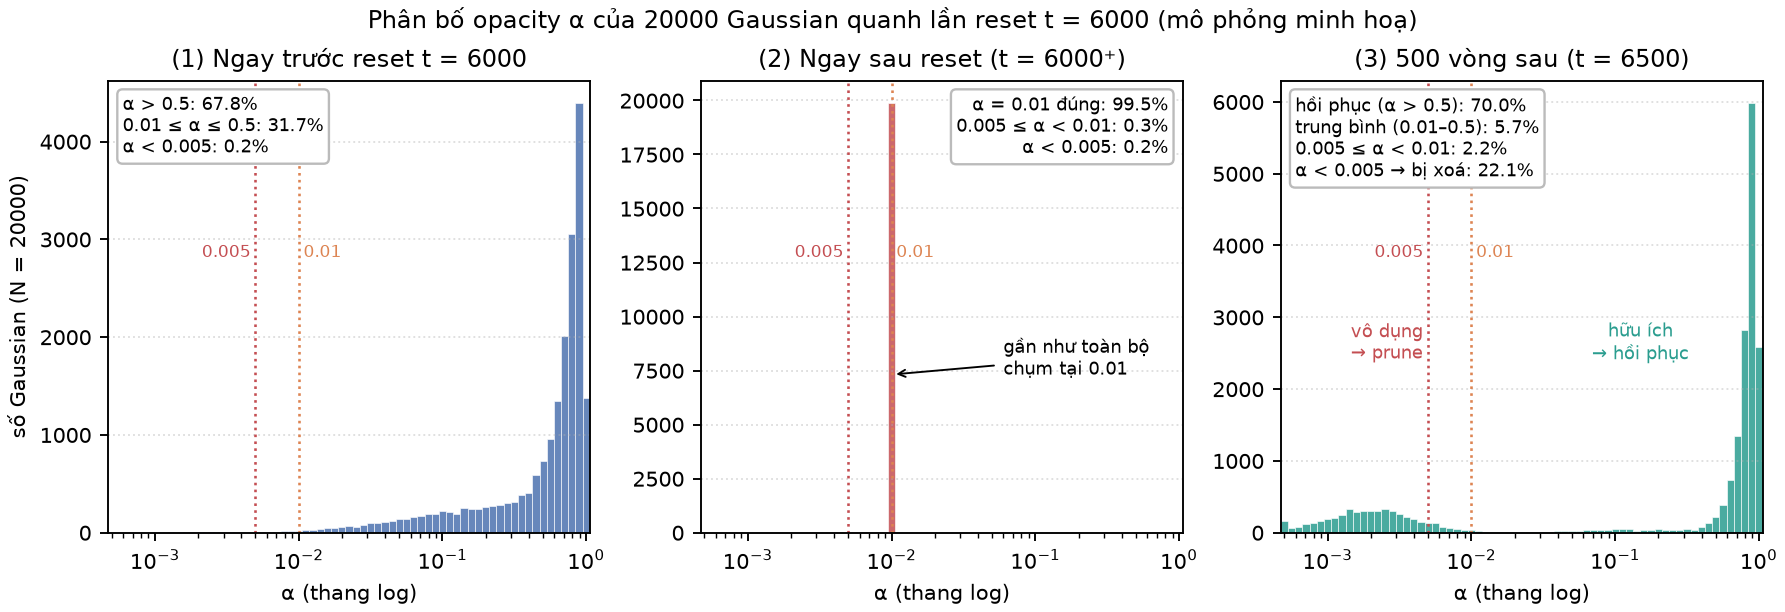
\includegraphics[width=0.8\linewidth]{fig_18_hist_reset.png}
\captionof{figure}{\footnotesize Ba histogram $\alpha$: trước reset, sau reset (dồn về $0.01$), $500$ vòng sau.}
\end{frame}


% ===================== PHẦN 5 =====================
\section{Ba đòn bẩy tăng tốc FastGS \& Mô hình chi phí}
% ============================================================
% PHẦN 5 (Slide 41--50): Quy trình Render 3D Gaussian Splatting
% và cải tiến FastGS -- Mô hình chi phí & ba đòn bẩy tăng tốc
% ============================================================

% --- Slide 41 ---
\begin{frame}{Vì sao 3DGS gốc chậm?}
\begin{itemize}
    \item Mỗi iteration huấn luyện gồm 4 khâu chính: \textbf{render} (chiếu + rasterize), \textbf{tính loss}, \textbf{backward} (lan truyền ngược), và định kỳ \textbf{densify/prune}.
    \item Với cảnh thực tế có hàng trăm nghìn đến hàng triệu Gaussian, chi phí \textbf{rasterize} và \textbf{backward} chiếm phần lớn thời gian mỗi bước.
    \item Densify/prune chỉ chạy định kỳ (không phải mỗi iteration) nhưng gây đột biến chi phí khi thực thi.
\end{itemize}
\vspace{0.3cm}
\centering
\footnotesize
\begin{tabular}{lcc}
\toprule
\textbf{Khâu} & \textbf{Tần suất} & \textbf{Tỉ trọng thời gian (ước lượng)} \\
\midrule
Render (project + rasterize) & mỗi iteration & \textasciitilde 45\% \\
Backward (gradient) & mỗi iteration & \textasciitilde 35\% \\
Tính loss & mỗi iteration & \textasciitilde 10\% \\
Densify/Prune & định kỳ & \textasciitilde 10\% (đột biến) \\
\bottomrule
\end{tabular}
\end{frame}

% --- Slide 42 ---
\begin{frame}{Định luật Amdahl áp dụng cho 3DGS}
\footnotesize
\begin{columns}[T]
\begin{column}{0.52\textwidth}
\begin{itemize}
    \item Tăng tốc một phần hệ thống chỉ mang lại lợi ích bị giới hạn bởi tỉ trọng thời gian phần đó chiếm trong toàn pipeline.
\end{itemize}
\begin{block}{Công thức Amdahl}
\[
\text{Speedup} = \dfrac{1}{(1-p) + \dfrac{p}{s}}
\]
\footnotesize $p$: tỉ trọng thời gian phần được tối ưu; $s$: hệ số tăng tốc riêng của phần đó.
\end{block}
\begin{itemize}
    \item Rasterize + backward chiếm $p$ lớn nhất $\Rightarrow$ FastGS tập trung tối ưu \textbf{đúng chỗ này}.
    \item Tối ưu phần chiếm $p$ nhỏ (vd.\ tính loss) dù $s$ lớn vẫn cho speedup tổng thể không đáng kể.
\end{itemize}
\end{column}
\begin{column}{0.48\textwidth}
\centering
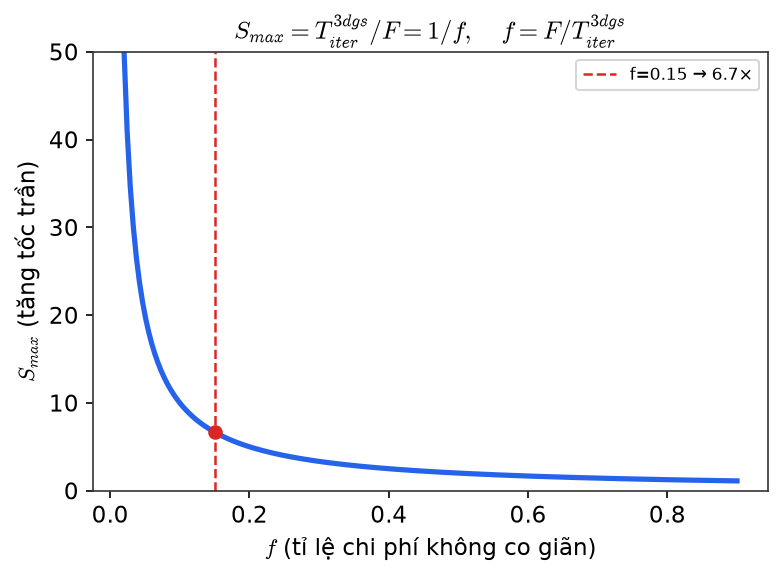
\includegraphics[width=0.95\linewidth]{ch8_amdahl.png}
\end{column}
\end{columns}
\end{frame}

% --- Slide 43 ---
\begin{frame}{Mô hình chi phí chi tiết của một iteration}
\footnotesize
\begin{columns}[T]
\begin{column}{0.52\textwidth}
\begin{itemize}
    \item Gọi $N$ là số Gaussian hiện có, $T_i$ là số tile mà Gaussian thứ $i$ chạm tới (tile\_touched).
\end{itemize}
\begin{block}{Chi phí rasterize}
\[
C_{\text{rasterize}} \sim O\!\left(\sum_{i=1}^{N} T_i\right) = O(N \times \overline{T})
\]
\footnotesize $\overline{T}$: số tile trung bình mỗi Gaussian chạm.
\end{block}
\begin{itemize}
    \item Chi phí densify/prune: $C_{\text{densify}} \sim O(N)$.
    \item Giảm $N$ (prune tốt hơn) hoặc giảm $\overline{T}$ (box nhỏ hơn) đều giảm trực tiếp chi phí -- cơ sở cho 2 trong 3 đòn bẩy của FastGS.
\end{itemize}
\end{column}
\begin{column}{0.48\textwidth}
\centering
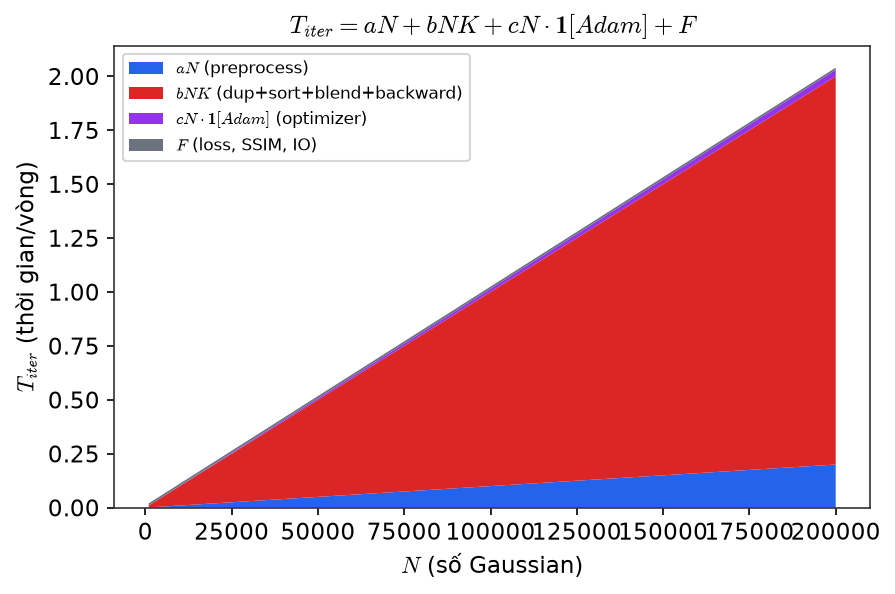
\includegraphics[width=0.95\linewidth]{ch8_cost_model.png}
\end{column}
\end{columns}
\end{frame}

% --- Slide 44 ---
\begin{frame}{Ba đòn bẩy tăng tốc của FastGS (tổng quan)}
\begin{columns}[t]
\column{0.33\linewidth}
\centering
\textbf{1. Multi-view score}
\begin{itemize}
    \footnotesize
    \item Đánh giá tầm quan trọng Gaussian qua nhiều góc nhìn
    \item Pruning thông minh hơn
\end{itemize}
\column{0.33\linewidth}
\centering
\textbf{2. Compact Box}
\begin{itemize}
    \footnotesize
    \item Giảm hệ số nhân bounding-box
    \item Giảm số tile mỗi Gaussian chạm
\end{itemize}
\column{0.33\linewidth}
\centering
\textbf{3. Sparse Adam}
\begin{itemize}
    \footnotesize
    \item Lịch cập nhật phân tầng
    \item Giảm tần suất optimizer.step()
\end{itemize}
\end{columns}
\vspace{0.4cm}
\begin{itemize}
    \item Cả ba đòn bẩy đều nhắm vào khâu chiếm tỉ trọng lớn nhất theo phân tích Amdahl: rasterize, densify/prune và cập nhật tham số.
\end{itemize}
\end{frame}

% --- Slide 45 ---
\begin{frame}{Đòn bẩy 1: Multi-view consistency score}
\begin{itemize}
    \item Cách cũ: điểm quan trọng của Gaussian dựa trên opacity/gradient tích luỹ từ \textbf{một} view tại một thời điểm -- dễ bị nhiễu do gradient cancellation (đã nêu ở Phần 4).
    \item FastGS tổng hợp đóng góp thực tế của Gaussian vào chất lượng ảnh qua \textbf{nhiều góc camera} trước khi quyết định prune/giữ.
\end{itemize}
\begin{block}{Điểm quan trọng tổng hợp}
\[
\text{Importance}(g) = \sum_{v \in \text{Views}} w_v \cdot \text{Contribution}(g, v)
\]
với $w_v$ là trọng số theo view (có thể đồng đều hoặc theo độ tin cậy).
\end{block}
\begin{itemize}
    \item Giải quyết trực tiếp vấn đề một view "khử" tín hiệu gradient của view khác, giúp pruning chính xác hơn, giảm $N$ hiệu quả hơn.
\end{itemize}
\end{frame}

% --- Slide 46 ---
\begin{frame}{Đòn bẩy 2: Compact Box multiplier}
\begin{itemize}
    \item Nhắc lại (Phần 2): bounding-box mặc định lấy theo $3\sigma$ của Gaussian để xác định vùng ảnh hưởng khi rasterize.
    \item FastGS giảm hệ số nhân \texttt{--mult} xuống \textbf{0.5} (cảnh nhỏ/vừa) hoặc \textbf{0.7} (cảnh lớn) thay vì 3.0 mặc định.
    \item Diện tích ellipse chiếu (và do đó số tile chạm $\overline{T}$) giảm theo bình phương hệ số nhân $\Rightarrow$ giảm trực tiếp $C_{\text{rasterize}}$.
    \item Đây là đòn bẩy \textbf{rẻ nhất} về mặt cài đặt (chỉ đổi 1 tham số) nhưng hiệu quả cao.
\end{itemize}
\vspace{0.2cm}
\centering
\footnotesize
\begin{tabular}{lcc}
\toprule
& \textbf{Mặc định (mult=3.0)} & \textbf{Compact box (mult=0.5--0.7)} \\
\midrule
Số tile trung bình/Gaussian & cao & thấp hơn đáng kể \\
Thời gian rasterize & baseline & giảm rõ rệt \\
\bottomrule
\end{tabular}
\end{frame}

% --- Slide 47 ---
\begin{frame}{Đòn bẩy 3: Sparse Adam schedule}
\begin{itemize}
    \item Nhắc lại (Phần 3): lịch step tối ưu hoá phân tầng theo bậc hệ số cầu điều hoà (SH).
    \item SH bậc cao: step mỗi 16 iteration cho đến 15k iteration đầu.
    \item Sau 15k: step mỗi 32 iteration; sau 20k: step mỗi 64 iteration cho các tham số ít quan trọng.
    \item Cơ sở: hệ số SH bậc cao biến thiên chậm sau giai đoạn đầu, gọi \texttt{optimizer.step()} dày đặc là lãng phí.
\end{itemize}
\vspace{0.2cm}
\centering
\footnotesize
\begin{tabular}{lcc}
\toprule
\textbf{Giai đoạn} & \textbf{Step đầy đủ (mỗi iter)} & \textbf{Sparse Adam} \\
\midrule
0 -- 15k & 15{,}000 lần & \textasciitilde 938 lần (/16) \\
15k -- 20k & 5{,}000 lần & \textasciitilde 156 lần (/32) \\
$>$20k & còn lại & /64 \\
\bottomrule
\end{tabular}
\begin{itemize}
    \item Chất lượng gần như không đổi, số lần gọi optimizer giảm mạnh $\Rightarrow$ giảm chi phí cập nhật tham số.
\end{itemize}
\end{frame}

% --- Slide 48 ---
\begin{frame}{Hiệu năng tích luỹ: Biểu đồ thác nước}
\footnotesize
\begin{itemize}
    \item Waterfall chart minh hoạ mức tăng tốc \textbf{tích luỹ} khi bật lần lượt từng đòn bẩy lên baseline 3DGS gốc.
    \item Thứ tự: baseline $\to$ + Compact Box $\to$ + Multi-view score $\to$ + Sparse Adam $\to$ FastGS đầy đủ.
    \item Mỗi đòn bẩy đóng góp độc lập, tổng hợp lại cho mức tăng tốc vượt trội so với chỉ áp dụng riêng lẻ.
\end{itemize}
\begin{center}
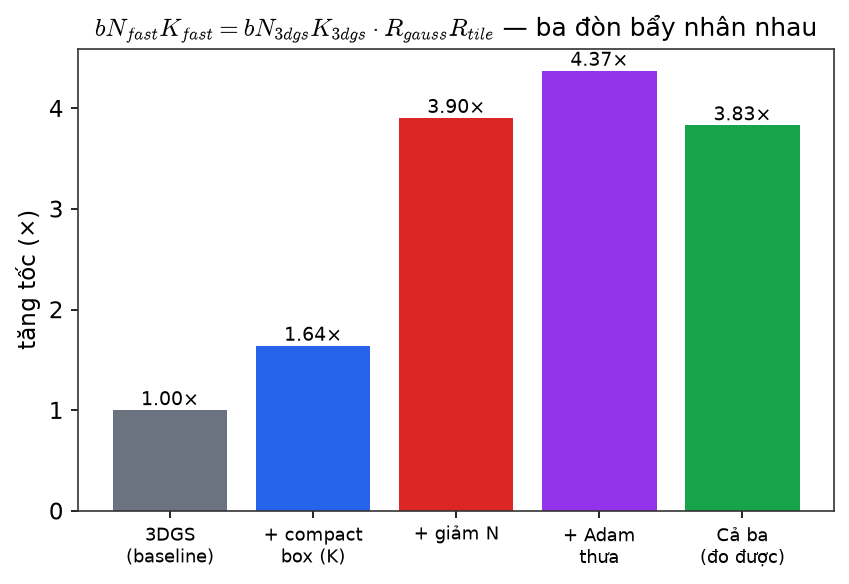
\includegraphics[width=0.68\linewidth]{ch8_levers_waterfall.png}
\end{center}
\end{frame}

% --- Slide 49 ---
\begin{frame}{Pipeline FastGS: ba đòn bẩy nằm ở đâu?}
\begin{center}
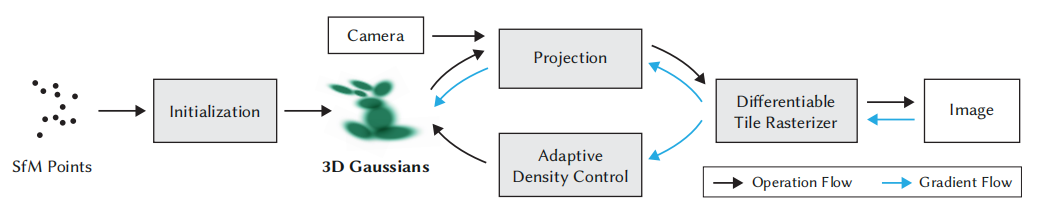
\includegraphics[width=0.95\linewidth]{pipe.png}
\end{center}
\begin{itemize}
    \footnotesize
    \item \textbf{Compact Box} $\to$ tác động tại bước \emph{rasterize} (giảm $\overline{T}$, giảm chi phí render).
    \item \textbf{Multi-view score} $\to$ tác động tại bước \emph{densify/prune} (chọn lọc Gaussian chính xác hơn).
    \item \textbf{Sparse Adam} $\to$ tác động tại bước \emph{optimizer step} (giảm tần suất cập nhật tham số).
\end{itemize}
\end{frame}

% --- Slide 50 ---
\begin{frame}{Tổng kết: từ 3DGS gốc đến FastGS}
\centering
\footnotesize
\begin{tabular}{lll}
\toprule
\textbf{Tham số} & \textbf{3DGS gốc} & \textbf{FastGS} \\
\midrule
\texttt{loss\_thresh} & không có & mới, 0.1 \\
\texttt{grad\_abs\_thresh} & gradient thường & Abs-GS, 0.0012 \\
\texttt{--dense} & cố định & 0.001--0.013 (theo scene extent) \\
\texttt{--highfeature\_lr} & lr chuẩn & 0.005--0.02 (chia thêm /20 trong code) \\
\texttt{--mult} (box multiplier) & 3.0 & 0.5--0.7 \\
\bottomrule
\end{tabular}
\vspace{0.4cm}
\begin{itemize}
    \item FastGS không thay đổi mô hình biểu diễn cảnh, mà tối ưu \textbf{tham số hoá} và \textbf{lịch huấn luyện} dựa trên mô hình chi phí và định luật Amdahl.
    \item Kết quả: tăng tốc đáng kể mà chất lượng tái tạo (PSNR/SSIM) gần như không đổi.
\end{itemize}
\end{frame}


% ===================== PHẦN 6 =====================
\section{FastGS-lite: Kết quả thực nghiệm trên Colab T4}
% ============================================================
% PHẦN 6 (Slide 51--60): FastGS-lite -- kết quả thực nghiệm
% ============================================================

% --- Slide 51 ---
\begin{frame}{FastGS-lite: từ 24GB RTX 4090 xuống Colab T4 miễn phí}
\begin{itemize}
    \item \textbf{fastgs-lite} là bản fork giữ nguyên thuật toán FastGS gốc, chỉ đóng gói lại để chạy trên phần cứng phổ thông (Colab T4 free tier).
    \item Không thay đổi công thức toán học hay pipeline huấn luyện -- chỉ thay đổi cách triển khai/vận hành.
\end{itemize}
\vspace{0.3em}
\footnotesize
\begin{table}
\centering
\begin{tabular}{lll}
\toprule
\textbf{Tiêu chí} & \textbf{FastGS gốc} & \textbf{fastgs-lite} \\
\midrule
Phần cứng mục tiêu & 24GB RTX 4090 & T4 ($\sim$15GB VRAM) + 12.7GB RAM \\
CUDA extension & git submodule & vendor sẵn trong repo (\texttt{git clone}) \\
Entry point & train.py + shell script & train.py + notebook có instrumentation \\
Tín hiệu tiến trình & L1 + EMA & Score tổng hợp, log mỗi 1000 iter \\
\bottomrule
\end{tabular}
\end{table}
\end{frame}

% --- Slide 52 ---
\begin{frame}{Ràng buộc phần cứng thực tế}
\begin{itemize}
    \item Colab T4 free tier: \textbf{14.56 GB VRAM}, nhưng RAM hệ thống (host) chỉ \textbf{12.7 GB}.
    \item Trực giác thông thường: nghẽn cổ chai sẽ ở VRAM (GPU). \textbf{Thực tế ngược lại}.
    \item VRAM peak đo được chỉ $\sim$1.16GB -- khoảng \textbf{8\%} dung lượng khả dụng.
    \item RAM peak đo được $\sim$9.59GB -- khoảng \textbf{91\%} giới hạn mềm 10.5GB của pipeline.
    \item[$\Rightarrow$] Phát hiện quan trọng, sẽ nhắc lại ở phần \emph{Quan sát} cuối bài: \textbf{RAM hệ thống, không phải VRAM, là ràng buộc thật sự}.
\end{itemize}
\vspace{0.5em}
\centering
\footnotesize
\begin{tabular}{lcc}
\toprule
 & VRAM (14.56GB) & RAM (12.7GB, soft limit 10.5GB) \\
\midrule
Peak sử dụng & 1.16GB (8\%) & 9.59GB (91\% soft limit) \\
\bottomrule
\end{tabular}
\end{frame}

% --- Slide 53 ---
\begin{frame}{Kiến trúc notebook: 7 cell $\leftrightarrow$ 7 module}
\footnotesize
\begin{table}
\centering
\begin{tabular}{cll}
\toprule
\textbf{Cell} & \textbf{Module} & \textbf{Chức năng} \\
\midrule
1 & \texttt{env.py} & Cài dependency, kiểm tra GPU \\
2 & \texttt{config.py} & Một object \texttt{Config} duy nhất cho toàn pipeline \\
3 & \texttt{data.py} & Tải dữ liệu, liệt kê scene \\
4 & \texttt{run.py} & Smoke test vài trăm iteration \\
5 & \texttt{trainer.py} + \texttt{score.py} & Train toàn bộ scene, log Score + \% tiến trình \\
6 & \texttt{report.py} & Bảng/biểu đồ phân tích kết quả \\
7 & \texttt{submission.py} + \texttt{deliver.py} & Đóng gói \texttt{submission.zip}, kiểm tra format, tự tải về \\
\bottomrule
\end{tabular}
\end{table}
\normalsize
\begin{itemize}
    \item Ánh xạ 1--1 giữa cell notebook và module trong \texttt{pipeline/} giúp dễ debug và tái sử dụng ngoài Colab.
\end{itemize}
\end{frame}

% --- Slide 54 ---
\begin{frame}{Thiết lập thực nghiệm}
\begin{itemize}
    \item 4 scene từ 2 dataset: \textbf{Deep Blending} (\texttt{drjohnson}, \texttt{playroom}) và \textbf{Tanks\&Temples} (\texttt{train}, \texttt{truck}).
    \item Split \texttt{--eval} với \texttt{llffhold=8} (cứ 8 ảnh lấy 1 làm test).
    \item Cấu hình tối ưu giống nhau mọi scene: \texttt{iterations=7000}, \texttt{sh\_degree=3}, \texttt{resolution=2} khi train.
    \item \textbf{Chú ý}: eval lại dùng độ phân giải gốc (\texttt{submission\_resolution=1}) -- sự lệch train/eval này do \emph{protocol cuộc thi}, không phải sơ suất.
\end{itemize}
\vspace{0.3em}
\footnotesize
\centering
\begin{tabular}{lcccc}
\toprule
\textbf{Scene} & \textbf{Cameras} & \textbf{Train views} & \textbf{Test views} & \textbf{Res. eval} \\
\midrule
drjohnson & -- & 7/8 & 1/8 & gốc (res=1) \\
playroom  & -- & 7/8 & 1/8 & gốc (res=1) \\
train     & -- & 7/8 & 1/8 & gốc (res=1) \\
truck     & -- & 7/8 & 1/8 & gốc (res=1) \\
\bottomrule
\end{tabular}
\end{frame}

% --- Slide 55 ---
\begin{frame}{Bảng 1: Chất lượng cuối cùng theo scene}
\footnotesize
\begin{table}
\centering
\begin{tabular}{lccccc}
\toprule
\textbf{Scene} & \textbf{Score} & \textbf{PSNR (dB)} & \textbf{SSIM} & \textbf{LPIPS} & \textbf{\#Gaussian} \\
\midrule
playroom  & 0.8198 & -- & -- & -- & $\sim$129k \\
drjohnson & 0.8027 & 27.41 & -- & -- & $\sim$174k \\
truck     & 0.7482 & -- & -- & -- & $\sim$187k \\
train     & 0.6867 & 19.75 & -- & -- & $\sim$201k \\
\midrule
\textbf{Mean} & \textbf{0.7643} & \textbf{24.46} & & & \\
\bottomrule
\end{tabular}
\end{table}
\begin{itemize}
    \item 2 scene indoor (playroom, drjohnson) vượt 2 scene outdoor (truck, train) dù dùng \textbf{ít Gaussian hơn} (129k--174k so với 187k--201k).
\end{itemize}
\centering
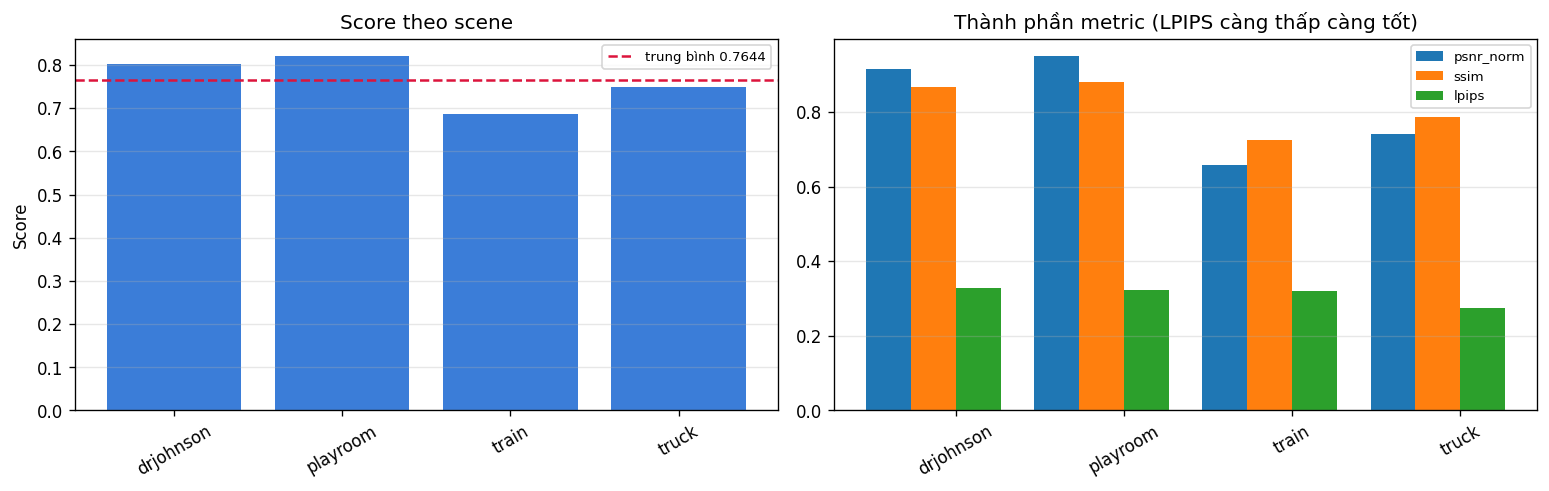
\includegraphics[width=0.55\linewidth]{leaderboard.png}
\captionof{figure}{Leaderboard Score theo scene}
\end{frame}

% --- Slide 56 ---
\begin{frame}{Bảng 2: Động lực huấn luyện}
\footnotesize
\begin{itemize}
    \item Score đo mỗi 1000 iteration trên cả 4 scene.
    \item Hai điểm sụt rõ rệt tại iteration \textbf{3000} và \textbf{6000}: Score rơi xuống $\sim$0.22--0.31.
    \item Trùng khớp chính xác với \texttt{opacity\_reset\_interval=3000}.
    \item[$\Rightarrow$] Đây là \textbf{hiện tượng đo lường} (measurement artifact) do lấy mẫu Score ngay lúc reset opacity, \textbf{không phải} mô hình phân kỳ. Phục hồi hoàn toàn trong dưới 1000 iteration sau đó.
\end{itemize}
\centering
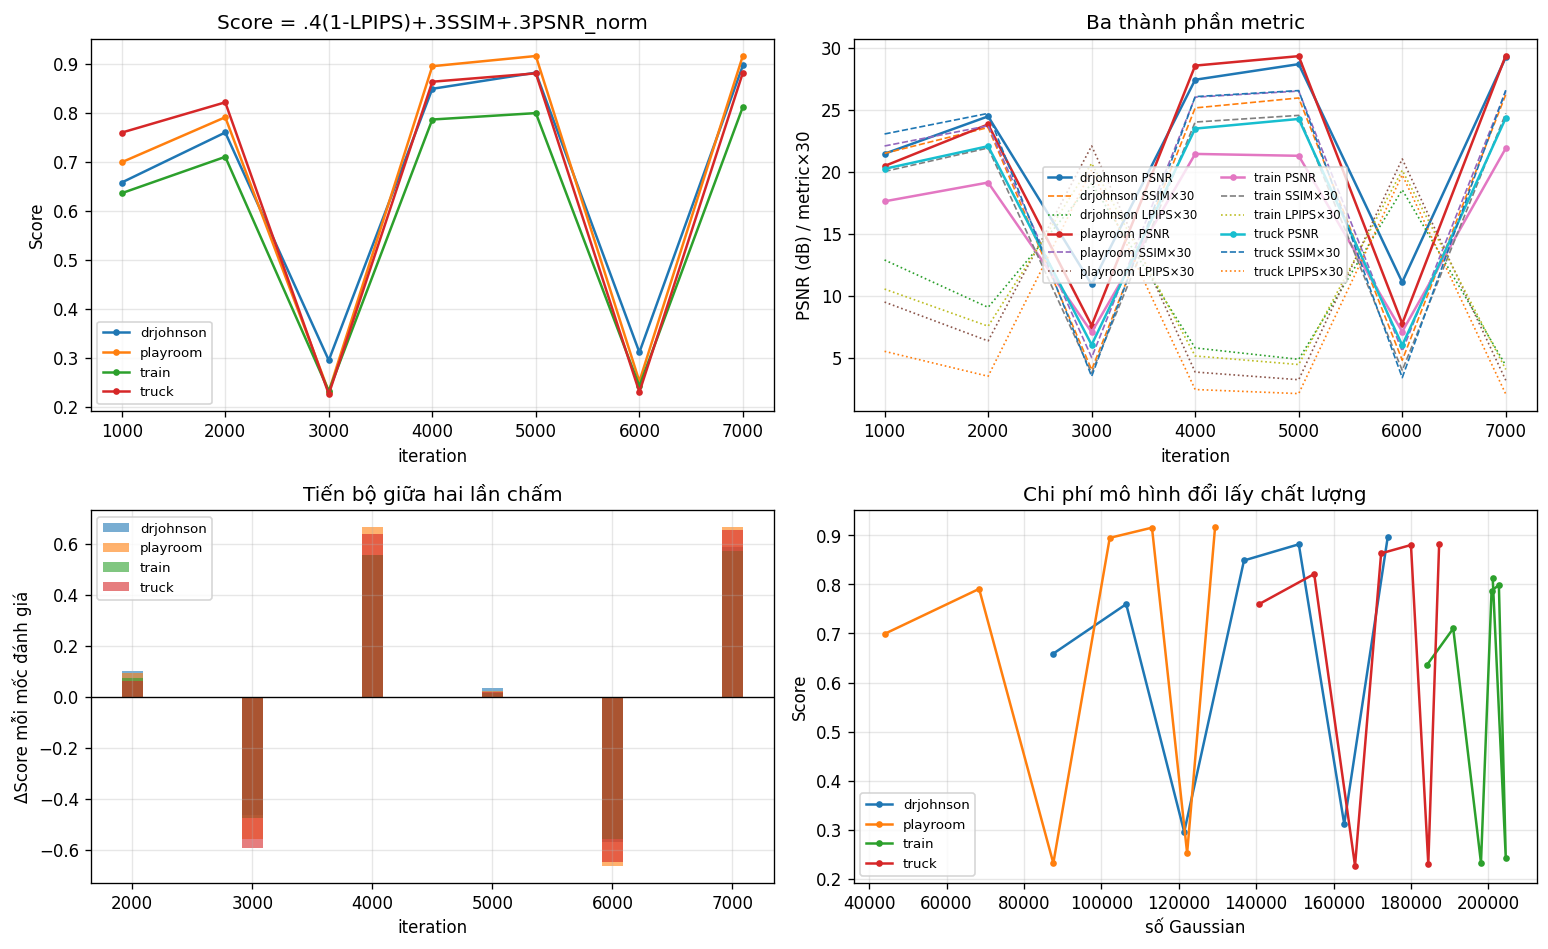
\includegraphics[width=0.48\linewidth]{training.png}
\captionof{figure}{\footnotesize Score theo iteration -- các điểm sụt tại 3000, 6000}
\end{frame}

% --- Slide 57 ---
\begin{frame}{Kết quả định tính: drjohnson (tốt nhất)}
\footnotesize
\begin{itemize}
    \item Score \textbf{0.8027}, PSNR \textbf{27.41dB}. Hình học, tư thế, màu sắc gần như khớp hoàn toàn với ground truth ở view đầu.
    \item Lỗi còn lại: chi tiết tần số cao / phụ thuộc góc nhìn -- chi tiết mảnh (khe tản nhiệt, gáy sách) bị mờ, highlight phản chiếu trên gỗ mahogany gần như biến mất.
    \item Nguyên nhân: các lobe SH bậc cao (view-dependent) có learning rate bị chia thêm \textbf{/20} trong code.
\end{itemize}
\centering
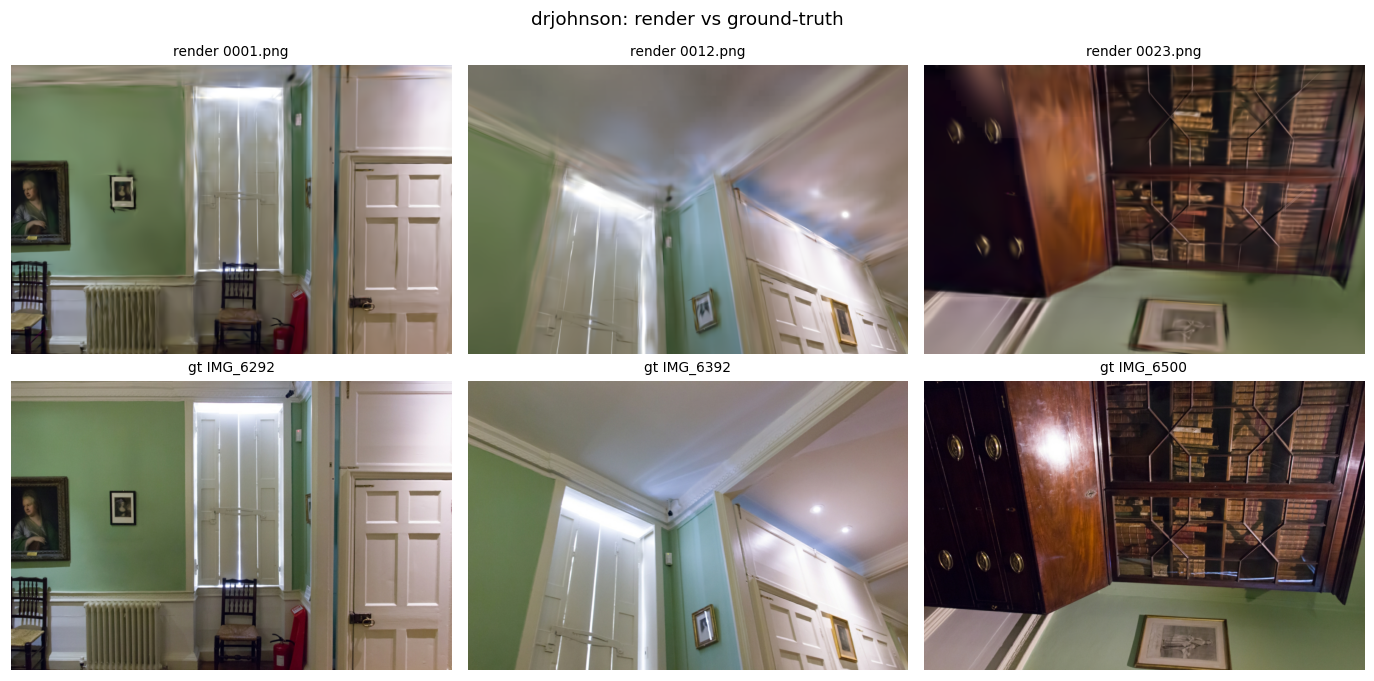
\includegraphics[width=0.5\linewidth]{samples_drjohnson.png}
\captionof{figure}{\footnotesize So sánh render vs. ground truth -- drjohnson}
\end{frame}

% --- Slide 58 ---
\begin{frame}{Kết quả định tính: train (yếu nhất -- vấn đề bầu trời)}
\footnotesize
\begin{itemize}
    \item Score \textbf{0.6867}, PSNR \textbf{19.75dB} -- thấp nhất trong 4 scene.
    \item Thất bại rõ rệt nhất: \textbf{vùng trời}. Ground truth là màu xanh đồng nhất, render lại đầy vệt xám-trắng loang lổ. Đầu máy xe lửa (có texture/parallax) tái tạo tốt.
    \item Vùng trời không texture, ở khoảng cách vô hạn, \textbf{không cho tín hiệu multi-view} nào để loại bỏ Gaussian dư thừa.
    \item[$\Rightarrow$] Giải thích vì sao lỗi rơi vào \textbf{PSNR} chứ không phải \textbf{LPIPS} (perceptual, ít nhạy vùng đồng nhất).
\end{itemize}
\centering
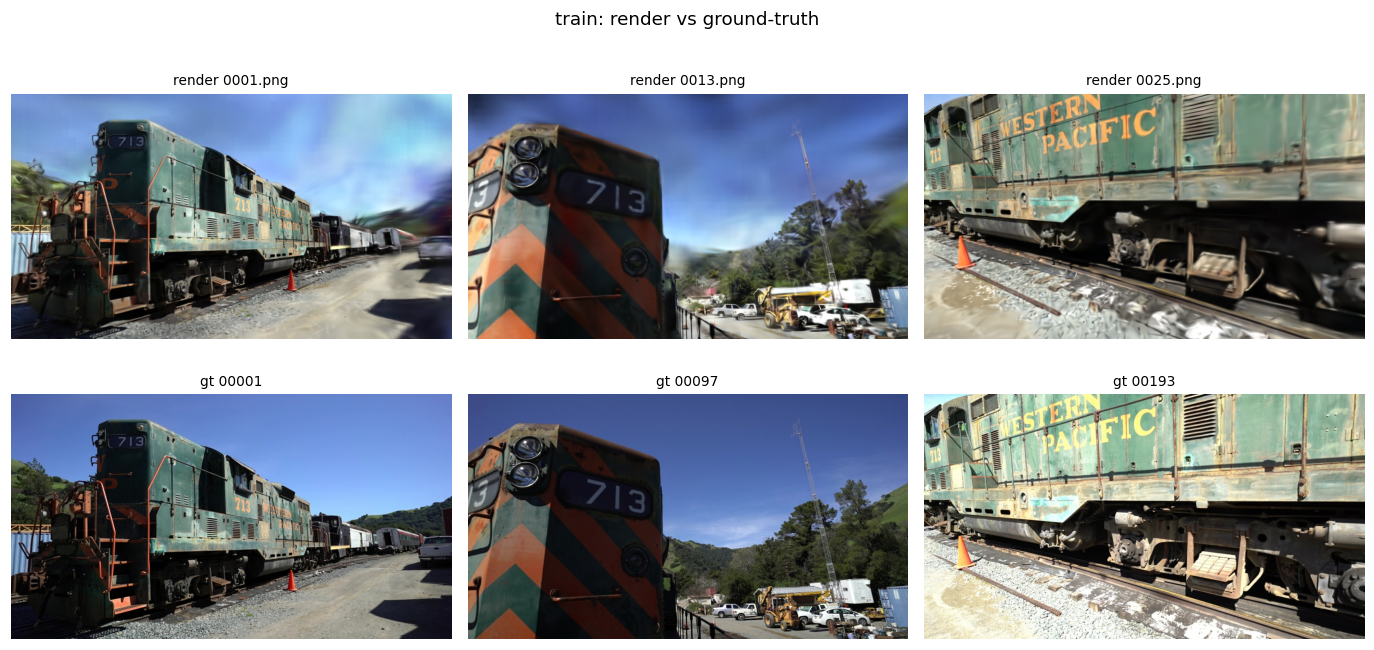
\includegraphics[width=0.5\linewidth]{samples_train.png}
\captionof{figure}{\footnotesize So sánh render vs. ground truth -- train (lỗi vùng trời)}
\end{frame}

% --- Slide 59 ---
\begin{frame}{Bảng 3: Chi phí \& lưu trữ}
\begin{itemize}
    \item Tổng thời gian train 4 scene: \textbf{327.6 giây} ($\sim$5.5 phút), tốc độ trung bình \textbf{85.5 iter/s}.
    \item VRAM đỉnh trung bình chỉ \textbf{0.88GB} (tối đa 1.16GB ở drjohnson) -- rất thấp so với 14.56GB khả dụng.
    \item Kích thước \texttt{point\_cloud.ply} trung bình \textbf{171.6MB} / 4 scene.
    \item Đúng \textbf{248 byte/Gaussian} = kích thước record 3DGS không nén (62 trường float32: 3 vị trí + 3 normal + 3 f\_dc + 45 f\_rest + 1 opacity + 3 scale + 4 rotation).
\end{itemize}
\vspace{0.3em}
\footnotesize
\centering
\begin{tabular}{lcc}
\toprule
\textbf{Chỉ số} & \textbf{Trung bình} & \textbf{Ghi chú} \\
\midrule
Thời gian train (4 scene) & 327.6 s & $\sim$5.5 phút tổng \\
Tốc độ & 85.5 iter/s & \\
VRAM peak & 0.88 GB & max 1.16GB (drjohnson) \\
Kích thước .ply & 171.6 MB & 248 byte/Gaussian \\
\bottomrule
\end{tabular}
\end{frame}

% --- Slide 60 ---
\begin{frame}{Khả năng tái lập \& giới hạn phép đo}
\footnotesize
\texttt{Config(resolution=2, iterations=7000, score\_every=1000,\\
\hspace{2em}eval\_views=6, psnr\_max=30.0, submission\_resolution=1)}
\normalsize
\vspace{0.5em}
\begin{itemize}
    \item \textbf{Giới hạn 1}: đây là \textbf{một lần chạy duy nhất}, không cố định seed, không lặp lại nhiều lần $\Rightarrow$ không có ước lượng phương sai/error bar.
    \item \textbf{Giới hạn 2}: chỉ 4 scene từ 2 dataset -- mẫu hẹp.
    \item \textbf{Giới hạn 3}: ngân sách 7k iteration chỉ bằng \textbf{1/3} lịch trình optimizer thiết kế cho 30k.
    \item \textbf{Giới hạn 4}: bỏ qua hoàn toàn bước prune cuối (\texttt{final\_prune\_fastgs}).
    \item[$\Rightarrow$] \textbf{Kết luận}: Bảng 1 nên xem là \emph{baseline có thể tái lập của repo này}, \textbf{không phải} kết quả benchmark chính thức để so sánh với FastGS/3DGS gốc.
\end{itemize}
\end{frame}


% ===================== PHẦN FASTER-GS (CVPR 2026) =====================
\section{Faster-GS (CVPR 2026): Cơ chế mới tích hợp}
% ============================================================
% PHẦN Faster-GS — Slide bổ sung 1/N: Tổng quan 5 cơ chế mới
% ============================================================

% --- Slide (mới) ---
\begin{frame}{Faster-GS (Hahlbohm et al., CVPR 2026): 5 cơ chế mới tích hợp}
\footnotesize
\begin{itemize}
    \item Repo vừa gộp thêm các cơ chế từ \textbf{Faster-GS} (Hahlbohm, Franke, Eisemann, Magnor — CVPR 2026) bên cạnh FastGS gốc, theo đúng tinh thần "luôn bật, không tuỳ chọn" (không còn cờ \texttt{if/else}).
\end{itemize}
\begin{table}
\centering
\begin{tabular}{ll}
\toprule
\textbf{Luôn bật (không cờ)} & \textbf{Giữ tắt (có chủ đích)} \\
\midrule
Fused Adam optimizer (kernel CUDA) & \\
3D anti-aliasing filter (Mip-Splatting) & MCMC densification \\
Morton Z-order reordering & \small (xung đột thuật toán với \\
Random-init fallback (thiếu COLMAP points3D) & \texttt{densify\_and\_prune\_fastgs}) \\
\bottomrule
\end{tabular}
\end{table}
\begin{itemize}
    \item MCMC densification là cơ chế thay thế đã cài đặt đầy đủ, đúng toán, nhưng \textbf{không được gọi} trong control-flow mặc định vì hai cơ chế densify không thể chạy đồng thời trên cùng tập Gaussian.
\end{itemize}
\centering
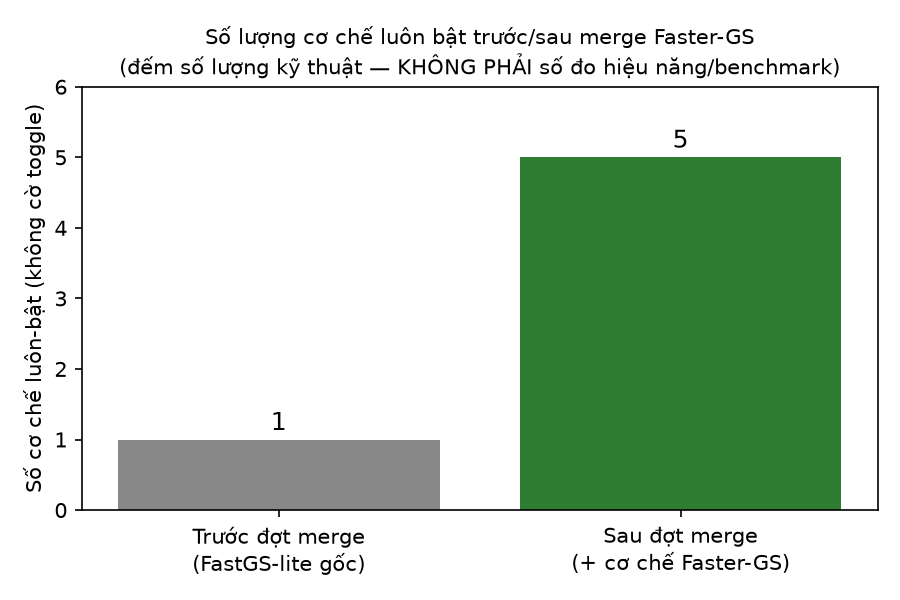
\includegraphics[width=0.3\linewidth]{../BOOK/fastergs_merge_figures/00_techniques_overview.png}
\captionof{figure}{\footnotesize Số cơ chế luôn bật trước/sau đợt merge (đếm số lượng, không phải benchmark)}
\end{frame}

% ============================================================
% PHẦN Faster-GS — Fused Adam optimizer
% ============================================================

% --- Slide: Fused Adam ---
\begin{frame}{Fused Adam optimizer — 1 kernel CUDA thay nhiều phép tensor}
\footnotesize
\begin{itemize}
    \item Công thức Adam chuẩn, không đổi thuật toán — chỉ đổi cách thực thi: 1 kernel CUDA elementwise (mỗi thread xử lý đúng 1 tham số, không phụ thuộc chéo $\Rightarrow$ không race condition) thay vì nhiều phép tensor/kernel-launch riêng lẻ của \texttt{torch.optim.Adam}.
\end{itemize}
\[
m_t=\beta_1 m_{t-1}+(1-\beta_1)g,\qquad v_t=\beta_2 v_{t-1}+(1-\beta_2)g^2
\]
\[
\hat m_t=\frac{m_t}{1-\beta_1^t},\qquad \hat v_t=\frac{v_t}{1-\beta_2^t},\qquad \theta_t=\theta_{t-1}-lr\cdot\frac{\hat m_t}{\sqrt{\hat v_t}+\epsilon}
\]
\begin{itemize}
    \item Tham số mặc định: $\beta_1=0.9$, $\beta_2=0.999$, $\epsilon=10^{-15}$.
    \item Lợi ích: giảm overhead kernel-launch, không phải giảm số phép toán $\Rightarrow$ kỳ vọng nhanh hơn chủ yếu ở chi phí launch, không phải ở độ phức tạp thuật toán.
    \item Luôn bật trong \texttt{GaussianModel.training\_setup} — không còn cờ toggle (\texttt{use\_fused\_adam} đã bị xoá).
    \item \alert{Cảnh báo:} chưa build/test trên GPU thật (không có CUDA toolchain khi phát triển) — cần build lại \texttt{diff-gaussian-rasterization\_fastgs} và so sánh output với \texttt{torch.optim.Adam} trước khi tin số liệu train.
\end{itemize}
\centering
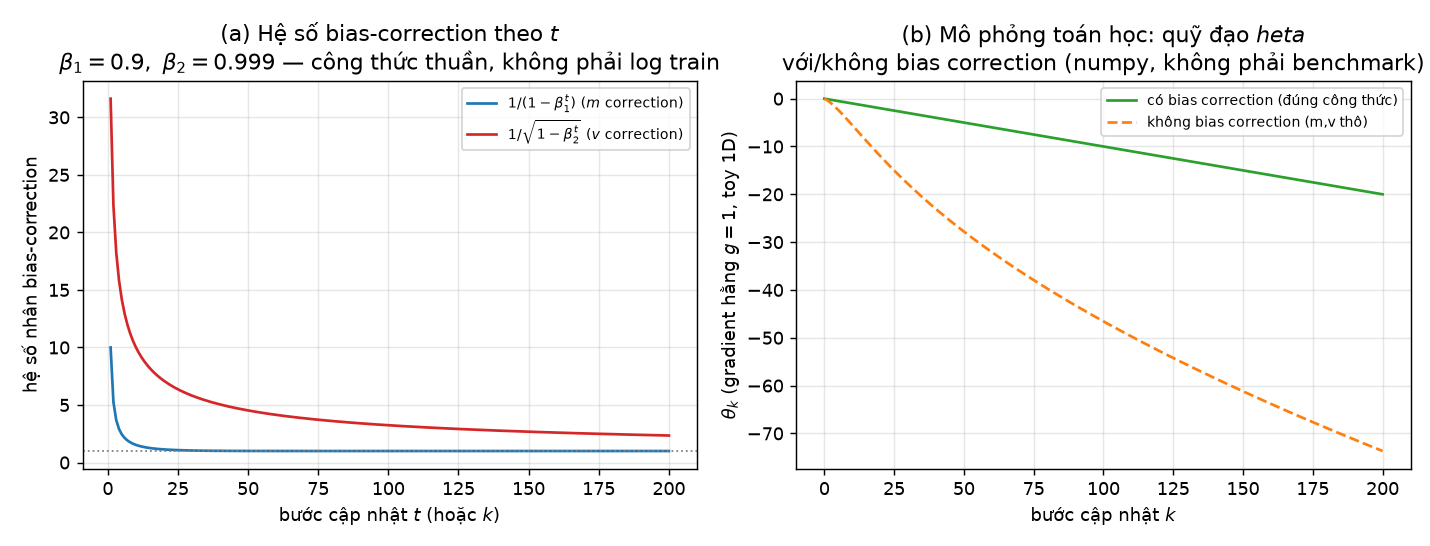
\includegraphics[width=0.42\linewidth]{11_adam_bias_correction.png}
\captionof{figure}{\footnotesize Hệ số bias-correction theo $t$ và mô phỏng quỹ đạo có/không hiệu chỉnh (công thức toán, không phải log train)}
\end{frame}

% ============================================================
% Faster-GS integration — 3D anti-aliasing filter (Mip-Splatting)
% ============================================================

% --- Slide: 3D anti-aliasing filter ---
\begin{frame}{3D anti-aliasing filter (Mip-Splatting) — luôn bật}
\footnotesize
\begin{itemize}
    \item Mỗi Gaussian sau projection phải có "dấu chân" tối thiểu $\sim$1 pixel để chống alias -- thực hiện bằng cách clamp scale trong log-space:
\end{itemize}
\[
s_{\text{final}} = \max(s_{\text{raw}}, \text{threshold}), \quad \text{threshold} = \text{distance2filter} \cdot z
\]
\begin{itemize}
    \item với $\text{distance2filter} = \sqrt{\text{filter\_variance}}/\text{max\_focal}$ (tính 1 lần từ toàn bộ camera train), $z$ = khoảng cách Gaussian tới camera.
    \item \textbf{Trực giác:} Gaussian càng xa camera, ngưỡng \texttt{threshold} càng lớn (vì $z$ lớn) $\Rightarrow$ scale tối thiểu tăng theo khoảng cách -- đúng với việc 1 pixel ở xa "bao phủ" vùng không gian lớn hơn.
    \item Trước đây có cờ \texttt{use\_3d\_filter} (mặc định \textbf{tắt}) -- giờ \textbf{luôn bật}, không còn cờ.
\end{itemize}
\centering
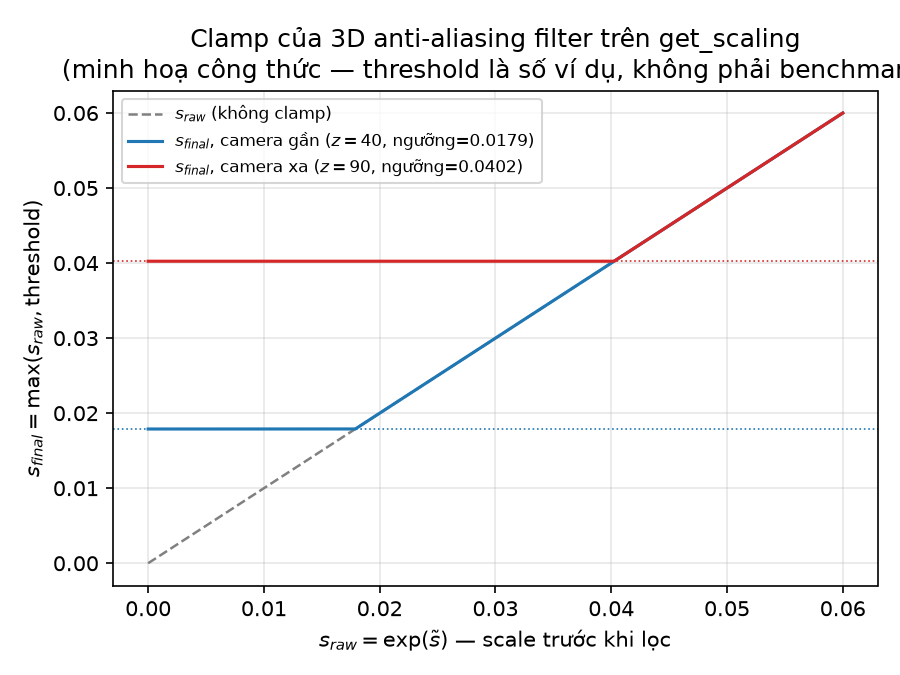
\includegraphics[width=0.3\linewidth]{07_3d_filter_clamp.png}
\captionof{figure}{\footnotesize Đường cong clamp $s_{\text{final}}=\max(s_{\text{raw}},\text{threshold})$ cho camera gần/xa (minh hoạ công thức, giá trị mẫu)}
\end{frame}

% ============================================================
% Faster-GS: Morton Z-order reordering
% ============================================================

\begin{frame}{Morton Z-order reordering --- tăng locality bộ nhớ}
\footnotesize
\begin{itemize}
    \item \textbf{Bước 1 --- Lượng tử hoá:} toạ độ mỗi Gaussian được đưa về 10 bit/trục trong bounding box của toàn bộ point cloud.
    \item \textbf{Bước 2 --- Spread bits (part1by2):} giãn mỗi số 10-bit thành 30-bit bằng magic-number bit trick, rồi ghép 3 trục:
    \[
        M = \text{spread}(q_x) \;\mathrel{\mathrm{OR}}\; \big(\text{spread}(q_y)\ll 1\big) \;\mathrel{\mathrm{OR}}\; \big(\text{spread}(q_z)\ll 2\big)
    \]
    \item \textbf{Bước 3 --- Sắp xếp:} toàn bộ Gaussian được \texttt{argsort} theo $M$ tăng dần --- đây chính là thứ tự duyệt theo \textbf{đường cong Z-order}: 2 điểm gần nhau trong không gian 3D thường có mã Morton gần nhau.
    \item[$\Rightarrow$] Gaussian trong cùng 1 tile màn hình thường gần nhau trong bộ nhớ sau reorder $\Rightarrow$ cache GPU hit rate cao hơn khi rasterizer tile-based duyệt danh sách Gaussian mỗi tile.
    \item Luôn chạy mỗi \texttt{morton\_reorder\_interval=5000} iteration (trước đây mặc định \texttt{0}, tức tắt hẳn).
\end{itemize}
\centering
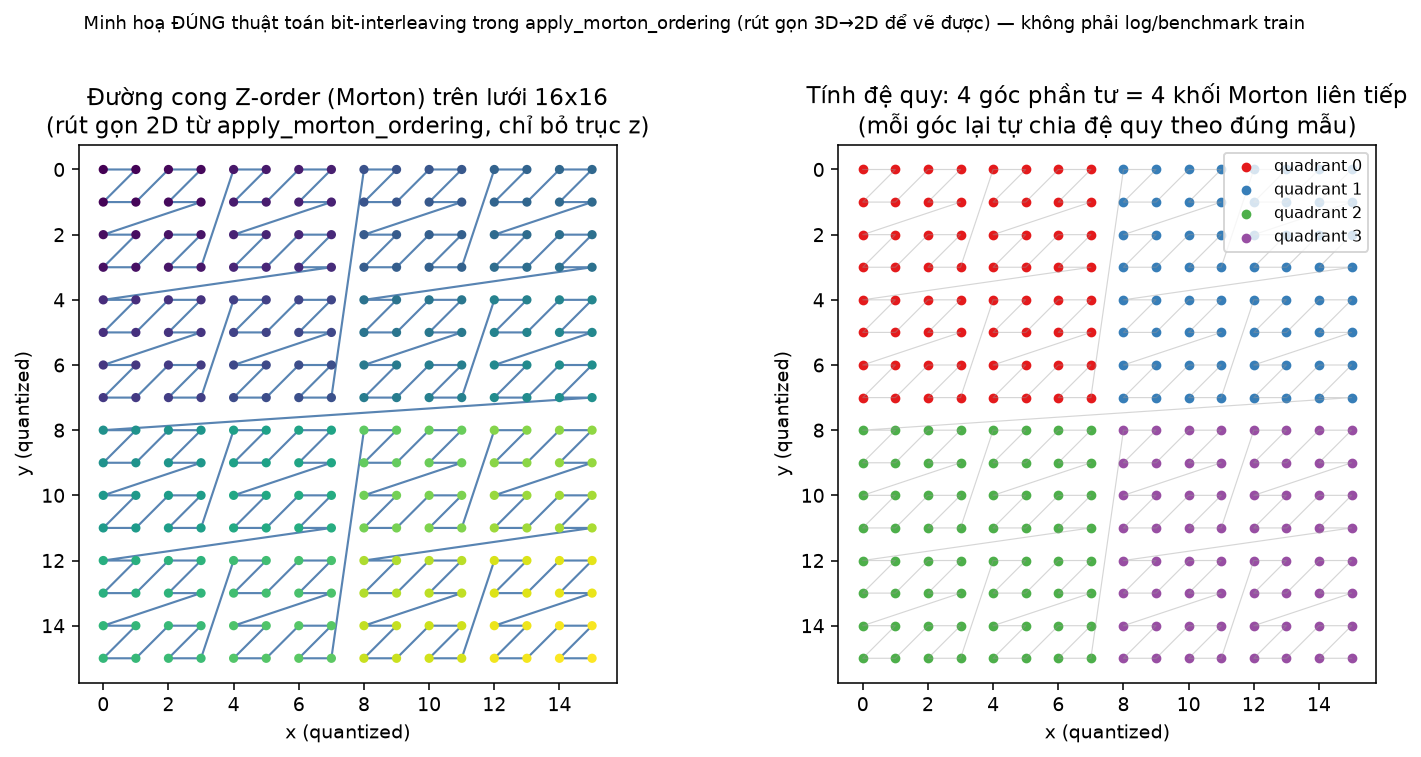
\includegraphics[width=0.38\linewidth]{../BOOK/fastergs_merge_figures/09_morton_zorder_curve.png}
\captionof{figure}{\footnotesize Đường cong Z-order thật (chạy đúng thuật toán spread-bits, rút gọn 3D$\to$2D để vẽ)}
\end{frame}

% ============================================================
% PHẦN Faster-GS bổ sung — Slide: MCMC densification (thay thế, không bật mặc định)
% ============================================================

% --- Slide (Faster-GS 5/8) ---
\begin{frame}{MCMC densification — có sẵn nhưng KHÔNG bật mặc định}
\footnotesize
\begin{itemize}
    \item Đây là phương án thay thế (\textbf{3DGS-MCMC}) cho densify chính của FastGS, đã cài đặt đầy đủ, đúng toán trong code -- nhưng \textbf{không} được gọi trong control-flow mặc định.
    \item Lý do: \alert{xung đột kiến trúc thật} -- MCMC và \texttt{densify\_and\_prune\_fastgs} loại trừ lẫn nhau, không thể chạy cùng lúc trên cùng tập Gaussian.
\end{itemize}
\vspace{0.3em}
\textbf{Closed-form relocation (3DGS-MCMC, Eq.\,9):} khi 1 Gaussian chết được thay bằng resample + nhân bản $n$ bản sao,
\[
\alpha' = 1-(1-\alpha)^{1/n}
\]
opacity mới mỗi bản sao, đảm bảo tổng hiệu ứng alpha-blending không đổi (khi $n=1$ thì $\alpha'=\alpha$).

\textbf{Noise injection:}
\[
\Delta xyz = lr\cdot\sigma(0.5-100\alpha)\cdot\Sigma\cdot\varepsilon
\]
Gaussian opacity thấp di chuyển nhiều hơn (khám phá), opacity cao gần như đứng yên.
\begin{itemize}
    \item[$\Rightarrow$] \texttt{densify\_and\_prune\_fastgs} (đóng góp chính của FastGS) vẫn là cơ chế densify duy nhất luôn bật; MCMC giữ nguyên trong code, sẵn sàng bật thủ công nếu muốn benchmark sau.
\end{itemize}
\centering
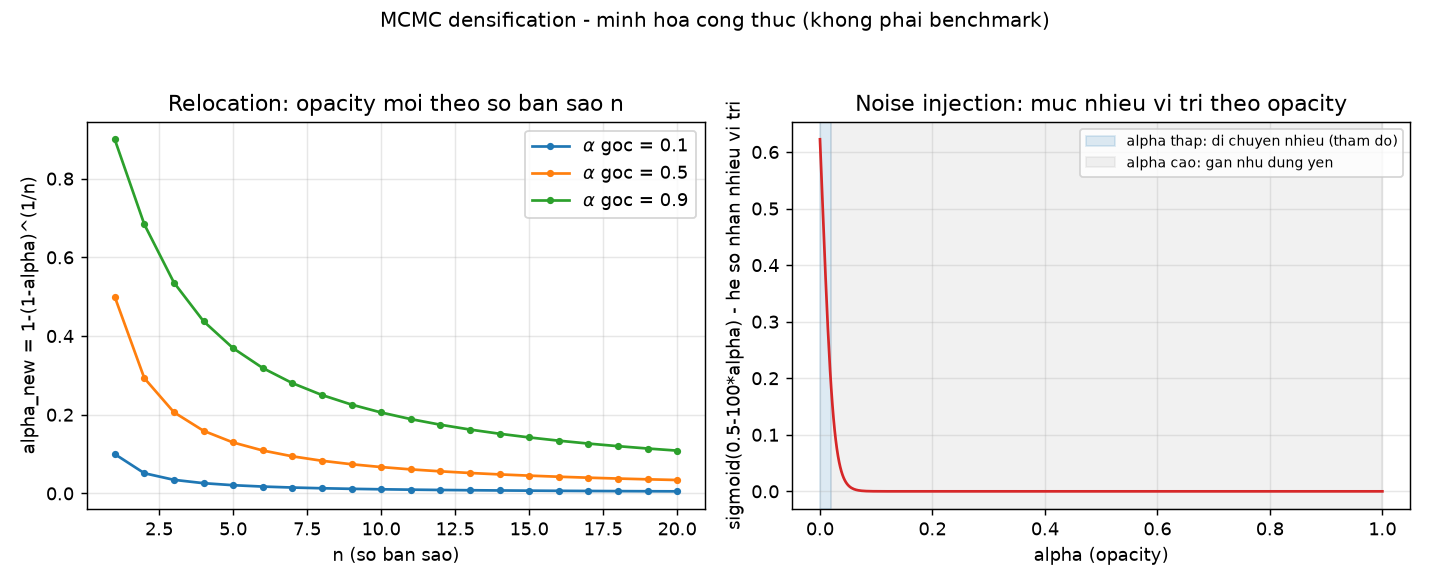
\includegraphics[width=0.38\linewidth]{../BOOK/adc_figures/12_mcmc_relocation_formula.png}
\captionof{figure}{\footnotesize $\alpha'$ theo $n$ và hệ số nhiễu sigmoid theo $\alpha$ (công thức toán, không phải benchmark)}
\end{frame}

% ============================================================
% PHẦN Faster-GS — Random-init fallback
% ============================================================

% --- Slide: Random-init fallback ---
\begin{frame}{Random-init fallback — khi COLMAP thiếu points3D}
\footnotesize
\begin{itemize}
    \item \textbf{Sample đều bên trong hình cầu} bán kính $R$ quanh tâm scene:
\end{itemize}
\[
r = R\cdot u^{1/3}, \qquad u\sim\text{Uniform}(0,1)
\]
\begin{itemize}
    \item Hướng lấy từ phân phối chuẩn rồi chuẩn hoá (đều trên mặt cầu đơn vị).
    \item \alert{Sai lầm thường gặp:} dùng $r=R\cdot u$ trực tiếp $\Rightarrow$ điểm dồn về tâm, vì thể tích vỏ cầu $dV\propto r^2\,dr$ — công thức $u^{1/3}$ mới cho mật độ \textbf{đều} trong toàn thể tích.
    \item \textbf{Frustum carving:} giữ điểm nếu nằm trong góc nhìn ít nhất 1 camera:
    \[
        z>0,\quad \lvert x\rvert\le z\tan(FovX/2),\quad \lvert y\rvert\le z\tan(FovY/2)
    \]
    Nếu carving xoá hết toàn bộ điểm $\Rightarrow$ fallback về tập chưa carve (an toàn, tránh crash).
    \item Chỉ kích hoạt khi COLMAP \textbf{không có} points3D dùng được (\texttt{random\_init\_force=False} mặc định) — không đổi hành vi khi COLMAP có sẵn dữ liệu.
\end{itemize}
\centering
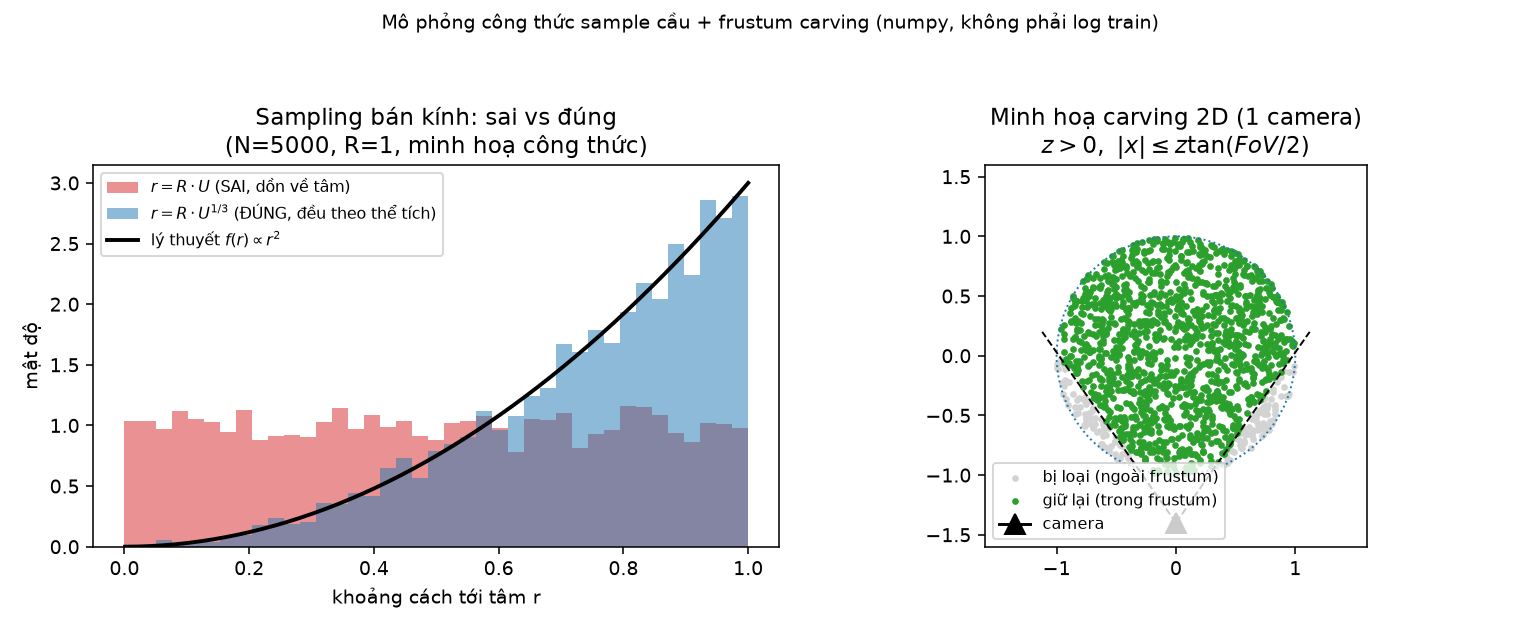
\includegraphics[width=0.38\linewidth]{06_random_init_sampling.png}
\captionof{figure}{\footnotesize Histogram thật so sánh 2 cách sample (đúng/sai) + minh hoạ carving 2D}
\end{frame}

% ============================================================
% Faster-GS integration — bug opacity_reset_interval đã sửa
% ============================================================

% --- Slide: Bug opacity_reset_interval đã sửa ---
\begin{frame}{Bug đã sửa: \texttt{opacity\_reset\_interval} không co giãn theo iterations}
\footnotesize
\begin{itemize}
    \item \textbf{Nguyên nhân thật} của các điểm sụt PSNR/Score tại iteration 3000/6000 (xem thêm Slide 56) -- \texttt{opacity\_reset\_interval} mặc định hardcode \textbf{3000} (đúng cho lịch gốc 30k iteration) \textbf{không co giãn} theo \texttt{iterations} thực tế đã rút ngắn (vd 7000) $\Rightarrow$ opacity reset kích hoạt quá sớm so với tiến trình densify (ở 43\% tiến trình thay vì đúng tỉ lệ).
    \item \textbf{Bằng chứng thật} (scene HCM0539, log \texttt{history.csv}): PSNR rơi $22.02\to5.92$, SSIM rơi $0.760\to0.047$ đúng tại iteration 3000.
    \item \textbf{Cách sửa}: field mới \texttt{opacity\_reset\_frac=0.2} trong \texttt{pipeline/config.py}; \texttt{pipeline/trainer.py::build\_args} giờ tính
    \[
    \texttt{opacity\_reset\_interval} = \text{round}(\texttt{opacity\_reset\_frac} \times \texttt{iterations})
    \]
    và truyền vào argv -- đồng bộ tỉ lệ với \texttt{densify\_until\_iter} (đã co giãn theo \texttt{densify\_until\_frac=0.5} từ trước).
    \item \alert{Lưu ý:} chưa có log thật "sau khi sửa" (chưa build/chạy lại vì không có GPU ở môi trường phát triển) -- chỉ có log thật "trước khi sửa" làm bằng chứng cho bug.
\end{itemize}
\centering
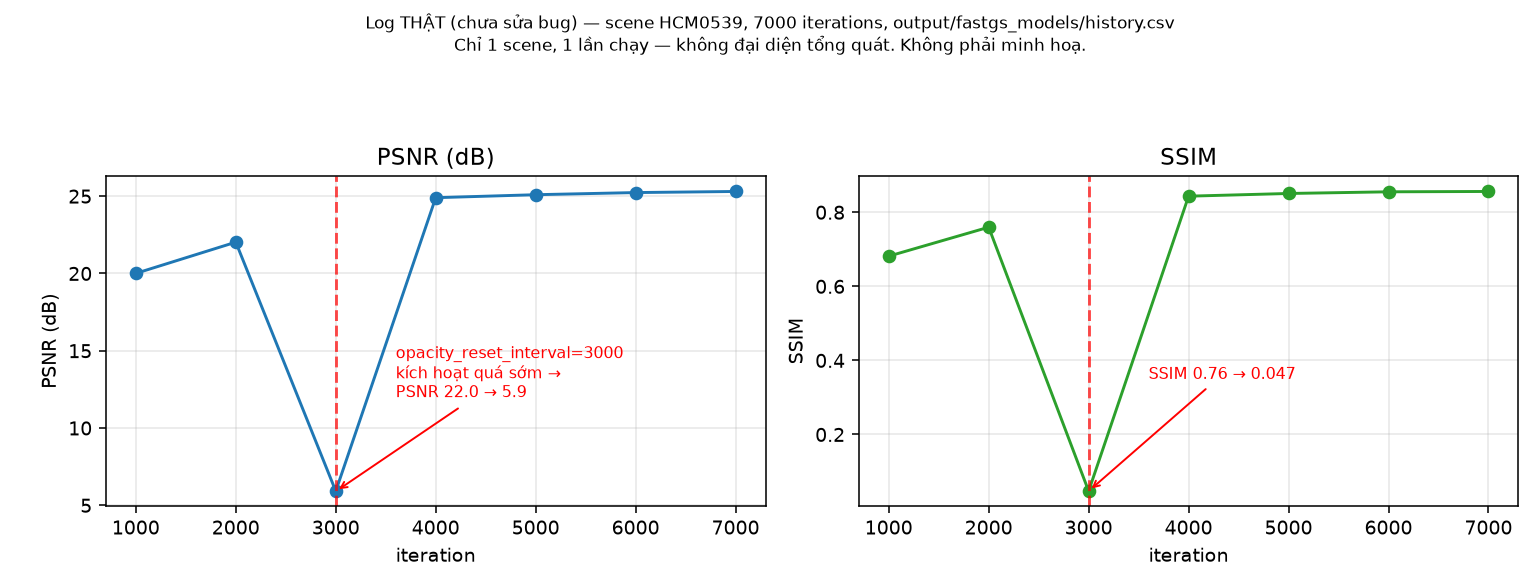
\includegraphics[width=0.35\linewidth]{12_opacity_reset_crash_real_log.png}
\captionof{figure}{\footnotesize Log thật (TRƯỚC khi sửa): PSNR sụp tại iteration 3000 -- 1 scene, 1 lần chạy}
\end{frame}

% ============================================================
% PHẦN Faster-GS — Slide bổ sung 8/8: Trạng thái kiểm định
% ============================================================

% --- Slide (mới) ---
\begin{frame}{Trạng thái kiểm định các cơ chế Faster-GS vừa tích hợp}
\footnotesize
\begin{itemize}
    \item Môi trường phát triển repo này \textbf{không có CUDA toolchain/GPU} $\Rightarrow$ mọi đánh giá dưới đây là \textbf{review tĩnh} (đọc code, đối chiếu công thức), chưa build/chạy thật.
\end{itemize}
\vspace{0.3em}
\begin{table}
\centering
\begin{tabular}{lccc}
\toprule
\textbf{Cơ chế} & \textbf{Review tĩnh} & \textbf{Build/compile GPU} & \textbf{Benchmark thật} \\
\midrule
Fused Adam optimizer & \textbf{Đã làm} & Chưa & Chưa \\
3D anti-aliasing filter & \textbf{Đã làm} & Chưa & Chưa \\
Morton reordering & \textbf{Đã làm} & Chưa & Chưa \\
Random-init fallback & \textbf{Đã làm} & Chưa & Chưa \\
Fix \texttt{opacity\_reset\_frac} & \textbf{Đã làm} & Chưa & Chưa \\
\bottomrule
\end{tabular}
\end{table}
\begin{itemize}
    \item \textbf{Việc user cần tự làm}: build lại \texttt{diff-gaussian-rasterization\_fastgs} (đã thêm \texttt{adam\_fused.cu} vào \texttt{setup.py}), chạy smoke test (\texttt{cfg.run\_smoke=True}, vài trăm iteration), so sánh \texttt{history.csv}/\texttt{leaderboard.csv} trước/sau đợt merge này.
    \item[$\Rightarrow$] Không có cơ chế nào trong bảng trên đã được \textbf{benchmark thật} — mọi khẳng định "nhanh hơn/ít VRAM hơn" hiện chỉ là suy luận tĩnh từ code, chưa phải kết quả đo.
\end{itemize}
\centering
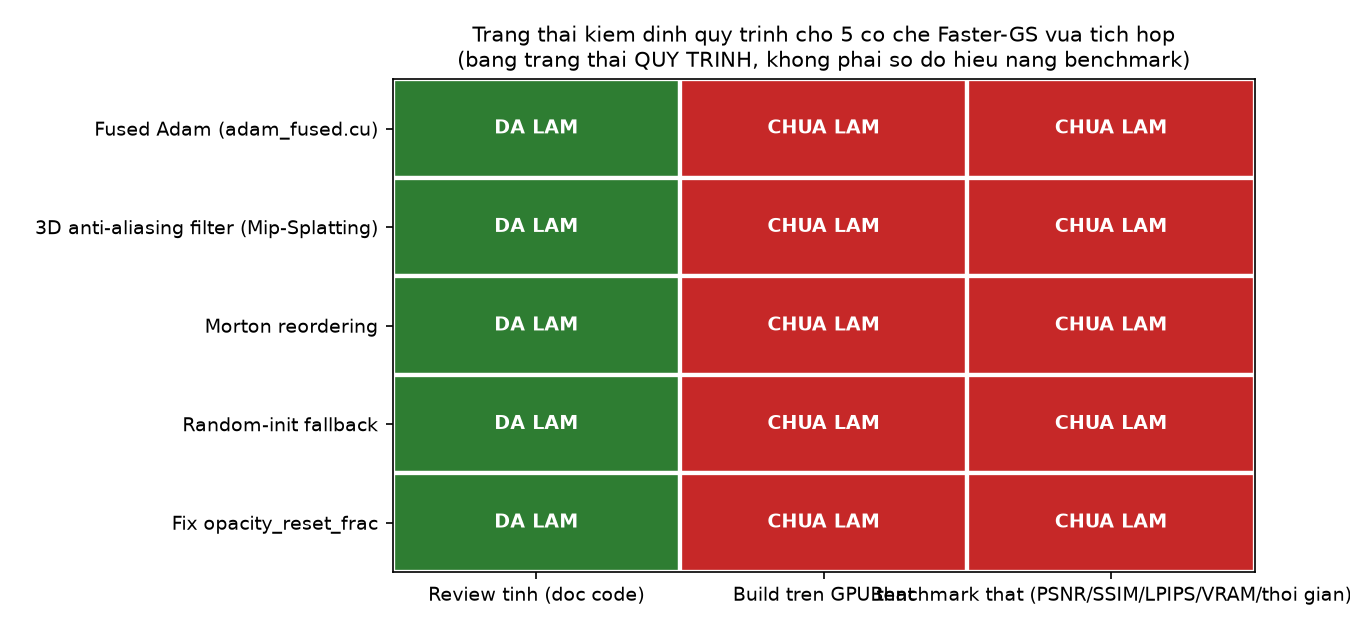
\includegraphics[width=0.3\linewidth]{15_verification_status.png}
\captionof{figure}{\footnotesize Bảng trạng thái kiểm định — không phải số đo hiệu năng}
\end{frame}


% ===================== PHẦN 7 =====================
\section{Quan sát \& Kết luận}
% ============================================================
% PHẦN 7 — Slide 61-67 (Quan sát bổ sung, Tổng kết, Q&A)
% ============================================================

% --- Slide 61 ---
\begin{frame}{Quan sát 1: \texttt{final\_prune} không kịp chạy ở 7k iteration}
\begin{itemize}
    \item Hàm \texttt{final\_prune\_fastgs} chỉ được phép chạy trong cửa sổ bảo vệ:
    \[
        15000 < \text{iteration} < 30000
    \]
    \item Một lần chạy chỉ với \textbf{7000 iteration} \textbf{không bao giờ} chạm tới cửa sổ này $\Rightarrow$ mô hình giao ra \textbf{chưa từng được prune cuối cùng}.
    \item Đây là lời giải thích khả dĩ nhất cho:
    \begin{itemize}
        \item Kích thước file lớn bất thường: \textbf{248 B/Gaussian}, hoàn toàn chưa nén.
        \item LPIPS "chững" quanh \textbf{0.31} thay vì tiếp tục cải thiện.
    \end{itemize}
    \item \alert{Hệ quả quan trọng:} mọi so sánh trực tiếp giữa số liệu 7k-iteration này với kết quả công bố gốc của FastGS/3DGS (chạy đủ 30k iteration) đều \textbf{không hợp lệ} — khác ngân sách huấn luyện, khác điểm dừng pipeline.
\end{itemize}
\end{frame}

% --- Slide 62 ---
\begin{frame}{Quan sát 2: Nút thắt là RAM hệ thống, không phải VRAM}
\begin{itemize}
    \item Đo trên Google Colab T4 trong quá trình huấn luyện:
\end{itemize}
\footnotesize
\begin{table}[]
\centering
\begin{tabular}{lccc}
\toprule
Tài nguyên & Đỉnh sử dụng & Khả dụng & \% sử dụng \\
\midrule
VRAM (GPU) & 1.16 GB & 14.56 GB & \textbf{8\%} \\
RAM hệ thống & 9.59 GB & 12.7 GB & \textbf{91\%} (giới hạn mềm 10.5 GB) \\
\bottomrule
\end{tabular}
\end{table}
\normalsize
\begin{itemize}
    \item RAM hệ thống áp sát giới hạn mềm của pipeline, trong khi VRAM còn dư rất nhiều.
    \item Khuyến nghị cũ "giảm độ phân giải để tiết kiệm VRAM" \textbf{không cần thiết} ở ngân sách này.
    \item \texttt{resolution=1} (độ phân giải gốc) hoàn toàn khả thi và còn loại bỏ luôn độ lệch train/eval resolution.
\end{itemize}
\end{frame}

% --- Slide 63 ---
\begin{frame}{Quan sát 3: Live-score vs reported-score — khác protocol, không phải suy giảm}
\begin{itemize}
    \item Score đo \textbf{trong lúc train} (live) cao hơn hẳn score \textbf{báo cáo cuối} (reported) — nhưng đây không phải mô hình bị tệ đi.
\end{itemize}
\footnotesize
\begin{table}[]
\centering
\begin{tabular}{lccc}
\toprule
Metric & Live (trong train) & Reported (cuối) & Chênh lệch \\
\midrule
PSNR (dB) & 26.23 & 24.46 & $-1.77$ \\
SSIM & 0.8675 & 0.8142 & $-0.0533$ (ít nhất) \\
LPIPS & 0.114 & 0.311 & $+0.197$ \\
\bottomrule
\end{tabular}
\end{table}
\normalsize
\begin{itemize}
    \item Nguyên nhân: (1) LPIPS backbone khác nhau — AlexNet lúc train vs VGG lúc báo cáo; (2) độ phân giải khác nhau — nửa độ phân giải lúc train vs độ phân giải gốc lúc báo cáo.
    \item \alert{Bài học:} không so sánh chéo hai protocol đo khác nhau khi đánh giá tiến bộ giữa các lần chạy.
\end{itemize}
\end{frame}

% --- Slide 64 ---
\begin{frame}{Tổng kết pipeline render 3D Gaussian Splatting}
\centering
\footnotesize
\begin{tikzpicture}[
    node distance=8mm and 6mm,
    box/.style={draw, rounded corners, align=center, minimum height=0.9cm, minimum width=2.6cm, fill=blue!8}
]
\node[box] (gauss) {3D Gaussian\\$(\mu,\Sigma,\alpha,SH)$};
\node[box, right=of gauss] (proj) {Chiếu phối cảnh\\(EWA)};
\node[box, right=of proj] (raster) {Rasterizer khả vi\\theo tile};

\node[box, below=of raster] (blend) {Alpha\\blending};
\node[box, left=of blend] (loss) {Loss\\($L_1$+D-SSIM)};
\node[box, left=of loss] (back) {Backward\\(gradient)};

\node[box, below=of back, fill=orange!12] (adc) {Adaptive\\Density Control};

\draw[-Latex] (gauss) -- (proj);
\draw[-Latex] (proj) -- (raster);
\draw[-Latex] (raster) -- (blend);
\draw[-Latex] (blend) -- (loss);
\draw[-Latex] (loss) -- (back);
\draw[-Latex] (back) -- (adc);
\draw[-Latex] (adc) -- (gauss);
\end{tikzpicture}
\vspace{2mm}

\normalsize
Một chu trình khép kín: render $\rightarrow$ tính loss $\rightarrow$ lan truyền ngược $\rightarrow$ điều chỉnh mật độ Gaussian $\rightarrow$ lặp lại.
\end{frame}

% --- Slide 65 ---
\begin{frame}{Tổng kết cải tiến FastGS \& giới hạn còn lại}
\textbf{Ba đòn bẩy chính và tác động:}
\begin{itemize}
    \item \textbf{Multi-view score} + \textbf{Compact box} $\Rightarrow$ giảm số Gaussian dư thừa mà không giảm chất lượng đáng kể.
    \item \textbf{Sparse Adam} $\Rightarrow$ giảm chi phí tính toán mỗi iteration (chỉ cập nhật tham số liên quan).
    \item \textbf{Mới:} tích hợp thêm 5 cơ chế từ \textbf{Faster-GS} (Hahlbohm et al., CVPR 2026) — fused Adam, 3D anti-aliasing filter, Morton reordering, random-init fallback (luôn bật), MCMC densification (có sẵn, giữ tắt) — xem phần Faster-GS mới trong bộ slide này để biết chi tiết công thức.
\end{itemize}
\vspace{2mm}
\textbf{Giới hạn / hướng phát triển:}
\begin{enumerate}
    \item Dữ liệu Gaussian đầu ra chưa được nén (248 B/Gaussian, thô).
    \item Ngân sách 7k iteration của fastgs-lite bỏ lỡ bước \texttt{final\_prune} (xem Slide 61).
    \item Chưa có ablation study cô lập riêng từng đòn bẩy để đo đóng góp thực tế của mỗi thành phần.
    \item 4 nhánh mở rộng của FastGS gốc — dynamic scenes, sparse view, surface reconstruction, SLAM — chưa được tích hợp vào fork này.
    \item Các cơ chế Faster-GS mới tích hợp mới chỉ được review tĩnh (đọc code), \textbf{CHƯA} build/benchmark thật trên GPU (không có CUDA toolchain khi phát triển).
\end{enumerate}
\end{frame}

% --- Slide 66 ---
\begin{frame}{Bản đồ tài liệu tham khảo}
\footnotesize
\begin{table}[]
\centering
\begin{tabular}{p{4.2cm}p{6.5cm}}
\toprule
\textbf{Tài liệu} & \textbf{Nội dung} \\
\midrule
\texttt{README.md} & Điểm vào tiếng Anh, bảng kết quả đầy đủ \\
\texttt{DOCS/fastgs-\allowbreak acceleration-\allowbreak method.md} & Nền tảng toán 3DGS + 3 đòn bẩy FastGS + đo FastGS-lite vs 3DGS \\
\texttt{DOCS/colab-t4-guide.md} & Playbook Colab T4, chống OOM, lộ trình CUDA \\
\texttt{DOCS/BOOK/} & Sách hợp nhất 15 chương, từ toán nền tảng tới cost model \\
\texttt{DOCS/BOOK/*\_merge\_figures/} & Biểu đồ minh hoạ công thức các cơ chế Faster-GS mới (fused Adam, 3D filter, Morton, MCMC, random-init) \\
GitHub & \texttt{KietAnhCS/fastgs-lite} \\
\bottomrule
\end{tabular}
\end{table}
\end{frame}

% --- Slide 67 ---
\begin{frame}[c]{}
\centering
{\Huge \textbf{Cảm ơn đã theo dõi!}}

\vspace{6mm}
{\LARGE Hỏi đáp (Q\&A)}

\vspace{10mm}
{\small Digital Twin GS --- FastGS-lite \\ \texttt{github.com/KietAnhCS/fastgs-lite}}
\end{frame}


\end{document}
